% Options for packages loaded elsewhere
% Options for packages loaded elsewhere
\PassOptionsToPackage{unicode}{hyperref}
\PassOptionsToPackage{hyphens}{url}
%
\documentclass[
  11pt,
  letterpaper,
]{book}
\usepackage{xcolor}
\usepackage[margin=2.5cm,paper=a4paper]{geometry}
\usepackage{amsmath,amssymb}
\setcounter{secnumdepth}{5}
\usepackage{iftex}
\ifPDFTeX
  \usepackage[T1]{fontenc}
  \usepackage[utf8]{inputenc}
  \usepackage{textcomp} % provide euro and other symbols
\else % if luatex or xetex
  \usepackage{unicode-math} % this also loads fontspec
  \defaultfontfeatures{Scale=MatchLowercase}
  \defaultfontfeatures[\rmfamily]{Ligatures=TeX,Scale=1}
\fi
\usepackage{lmodern}
\ifPDFTeX\else
  % xetex/luatex font selection
\fi
% Use upquote if available, for straight quotes in verbatim environments
\IfFileExists{upquote.sty}{\usepackage{upquote}}{}
\IfFileExists{microtype.sty}{% use microtype if available
  \usepackage[]{microtype}
  \UseMicrotypeSet[protrusion]{basicmath} % disable protrusion for tt fonts
}{}
\makeatletter
\@ifundefined{KOMAClassName}{% if non-KOMA class
  \IfFileExists{parskip.sty}{%
    \usepackage{parskip}
  }{% else
    \setlength{\parindent}{0pt}
    \setlength{\parskip}{6pt plus 2pt minus 1pt}}
}{% if KOMA class
  \KOMAoptions{parskip=half}}
\makeatother
% Make \paragraph and \subparagraph free-standing
\makeatletter
\ifx\paragraph\undefined\else
  \let\oldparagraph\paragraph
  \renewcommand{\paragraph}{
    \@ifstar
      \xxxParagraphStar
      \xxxParagraphNoStar
  }
  \newcommand{\xxxParagraphStar}[1]{\oldparagraph*{#1}\mbox{}}
  \newcommand{\xxxParagraphNoStar}[1]{\oldparagraph{#1}\mbox{}}
\fi
\ifx\subparagraph\undefined\else
  \let\oldsubparagraph\subparagraph
  \renewcommand{\subparagraph}{
    \@ifstar
      \xxxSubParagraphStar
      \xxxSubParagraphNoStar
  }
  \newcommand{\xxxSubParagraphStar}[1]{\oldsubparagraph*{#1}\mbox{}}
  \newcommand{\xxxSubParagraphNoStar}[1]{\oldsubparagraph{#1}\mbox{}}
\fi
\makeatother
\usepackage{fancyvrb}

\usepackage{color}
\usepackage{fancyvrb}
\newcommand{\VerbBar}{|}
\newcommand{\VERB}{\Verb[commandchars=\\\{\}]}
\DefineVerbatimEnvironment{Highlighting}{Verbatim}{commandchars=\\\{\}}
% Add ',fontsize=\small' for more characters per line
\usepackage{framed}
\definecolor{shadecolor}{RGB}{241,243,245}
\newenvironment{Shaded}{\begin{snugshade}}{\end{snugshade}}
\newcommand{\AlertTok}[1]{\textcolor[rgb]{0.68,0.00,0.00}{#1}}
\newcommand{\AnnotationTok}[1]{\textcolor[rgb]{0.37,0.37,0.37}{#1}}
\newcommand{\AttributeTok}[1]{\textcolor[rgb]{0.40,0.45,0.13}{#1}}
\newcommand{\BaseNTok}[1]{\textcolor[rgb]{0.68,0.00,0.00}{#1}}
\newcommand{\BuiltInTok}[1]{\textcolor[rgb]{0.00,0.23,0.31}{#1}}
\newcommand{\CharTok}[1]{\textcolor[rgb]{0.13,0.47,0.30}{#1}}
\newcommand{\CommentTok}[1]{\textcolor[rgb]{0.37,0.37,0.37}{#1}}
\newcommand{\CommentVarTok}[1]{\textcolor[rgb]{0.37,0.37,0.37}{\textit{#1}}}
\newcommand{\ConstantTok}[1]{\textcolor[rgb]{0.56,0.35,0.01}{#1}}
\newcommand{\ControlFlowTok}[1]{\textcolor[rgb]{0.00,0.23,0.31}{\textbf{#1}}}
\newcommand{\DataTypeTok}[1]{\textcolor[rgb]{0.68,0.00,0.00}{#1}}
\newcommand{\DecValTok}[1]{\textcolor[rgb]{0.68,0.00,0.00}{#1}}
\newcommand{\DocumentationTok}[1]{\textcolor[rgb]{0.37,0.37,0.37}{\textit{#1}}}
\newcommand{\ErrorTok}[1]{\textcolor[rgb]{0.68,0.00,0.00}{#1}}
\newcommand{\ExtensionTok}[1]{\textcolor[rgb]{0.00,0.23,0.31}{#1}}
\newcommand{\FloatTok}[1]{\textcolor[rgb]{0.68,0.00,0.00}{#1}}
\newcommand{\FunctionTok}[1]{\textcolor[rgb]{0.28,0.35,0.67}{#1}}
\newcommand{\ImportTok}[1]{\textcolor[rgb]{0.00,0.46,0.62}{#1}}
\newcommand{\InformationTok}[1]{\textcolor[rgb]{0.37,0.37,0.37}{#1}}
\newcommand{\KeywordTok}[1]{\textcolor[rgb]{0.00,0.23,0.31}{\textbf{#1}}}
\newcommand{\NormalTok}[1]{\textcolor[rgb]{0.00,0.23,0.31}{#1}}
\newcommand{\OperatorTok}[1]{\textcolor[rgb]{0.37,0.37,0.37}{#1}}
\newcommand{\OtherTok}[1]{\textcolor[rgb]{0.00,0.23,0.31}{#1}}
\newcommand{\PreprocessorTok}[1]{\textcolor[rgb]{0.68,0.00,0.00}{#1}}
\newcommand{\RegionMarkerTok}[1]{\textcolor[rgb]{0.00,0.23,0.31}{#1}}
\newcommand{\SpecialCharTok}[1]{\textcolor[rgb]{0.37,0.37,0.37}{#1}}
\newcommand{\SpecialStringTok}[1]{\textcolor[rgb]{0.13,0.47,0.30}{#1}}
\newcommand{\StringTok}[1]{\textcolor[rgb]{0.13,0.47,0.30}{#1}}
\newcommand{\VariableTok}[1]{\textcolor[rgb]{0.07,0.07,0.07}{#1}}
\newcommand{\VerbatimStringTok}[1]{\textcolor[rgb]{0.13,0.47,0.30}{#1}}
\newcommand{\WarningTok}[1]{\textcolor[rgb]{0.37,0.37,0.37}{\textit{#1}}}

\usepackage{longtable,booktabs,array}
\usepackage{calc} % for calculating minipage widths
% Correct order of tables after \paragraph or \subparagraph
\usepackage{etoolbox}
\makeatletter
\patchcmd\longtable{\par}{\if@noskipsec\mbox{}\fi\par}{}{}
\makeatother
% Allow footnotes in longtable head/foot
\IfFileExists{footnotehyper.sty}{\usepackage{footnotehyper}}{\usepackage{footnote}}
\makesavenoteenv{longtable}
\usepackage{graphicx}
\makeatletter
\newsavebox\pandoc@box
\newcommand*\pandocbounded[1]{% scales image to fit in text height/width
  \sbox\pandoc@box{#1}%
  \Gscale@div\@tempa{\textheight}{\dimexpr\ht\pandoc@box+\dp\pandoc@box\relax}%
  \Gscale@div\@tempb{\linewidth}{\wd\pandoc@box}%
  \ifdim\@tempb\p@<\@tempa\p@\let\@tempa\@tempb\fi% select the smaller of both
  \ifdim\@tempa\p@<\p@\scalebox{\@tempa}{\usebox\pandoc@box}%
  \else\usebox{\pandoc@box}%
  \fi%
}
% Set default figure placement to htbp
\def\fps@figure{htbp}
\makeatother

\ifLuaTeX
  \usepackage{luacolor}
  \usepackage[soul]{lua-ul}
\else
  \usepackage{soul}
\fi




\setlength{\emergencystretch}{3em} % prevent overfull lines

\providecommand{\tightlist}{%
  \setlength{\itemsep}{0pt}\setlength{\parskip}{0pt}}



 
\usepackage[]{biblatex}
\addbibresource{ref/MAref.bib}


% AMTAIR Thesis Preamble - Zero package conflicts
% Only formatting commands, no package loading

% Line spacing for academic work
\usepackage{setspace}
\onehalfspacing

% Custom chapter formatting (remove "Chapter N" prefix) but unfortunately leaves blank space
\usepackage{titlesec}
\titleformat{\chapter}[display]
  {\normalfont\huge\bfseries}  % format
  {}                           % label (empty = no "Chapter N")
  {0pt}                        % sep
  {\Huge}                      % before-code



% Page formatting and headers
\usepackage{fancyhdr}
\pagestyle{fancy}
\fancyhf{}
\fancyhead[LE,RO]{\slshape\nouppercase{\rightmark}}
\fancyhead[LO,RE]{\slshape\nouppercase{\leftmark}}
\fancyfoot[C]{\thepage}

% % Fix page breaks after title page
% \newcommand{\cleartitlepage}{
%   \clearpage
%   \thispagestyle{empty}
%   \mbox{}
%   \clearpage
% }



\renewcommand{\maketitle}{}

%  Citation customization
% \usepackage[style=authoryear,backend=biber,natbib=true]{biblatex}

% % Custom citation commands for different contexts
% \newcommand{\citeauthor}[1]{\textcite{#1}}           % Author (year)
% \newcommand{\citeyear}[1]{(\citeyear*{#1})}         % (year)
% \newcommand{\citealt}[1]{\citeauthor{#1} \citeyear{#1}}  % Author year
% \newcommand{\citep}[1]{(\cite{#1})}                 # (Author, year)

% Page reference styling
% \DeclareFieldFormat{postnote}{#1}                    # No "p." prefix
% \DeclareFieldFormat{multipostnote}{#1}               # No "pp." prefix


% % Page numbering control
% \usepackage{afterpage}

% % Command to start front matter (roman numerals)
% \newcommand{\frontmatter}{
%   \cleardoublepage
%   \pagenumbering{roman}
%   \setcounter{page}{1}
% }

% % Command to start main matter (arabic numerals)
% \newcommand{\mainmatter}{
%   \cleardoublepage
%   \pagenumbering{arabic}
%   \setcounter{page}{1}
% }

% % Command to start back matter (continue arabic)
% \newcommand{\backmatter}{
%   \cleardoublepage
%   % Keep arabic numbering but could change style if needed
% }

% % Suppress page numbers on title page
% \newcommand{\titlepage}{
%   \thispagestyle{empty}
% }



% Commands for custom title page
% \newcommand{\thesistitle}{Automating the Modelling of Transformative Artificial Intelligence Risks}
% \newcommand{\thesisauthor}{Valentin Jakob Meyer}
\makeatletter
\@ifpackageloaded{tcolorbox}{}{\usepackage[skins,breakable]{tcolorbox}}
\@ifpackageloaded{fontawesome5}{}{\usepackage{fontawesome5}}
\definecolor{quarto-callout-color}{HTML}{909090}
\definecolor{quarto-callout-note-color}{HTML}{0758E5}
\definecolor{quarto-callout-important-color}{HTML}{CC1914}
\definecolor{quarto-callout-warning-color}{HTML}{EB9113}
\definecolor{quarto-callout-tip-color}{HTML}{00A047}
\definecolor{quarto-callout-caution-color}{HTML}{FC5300}
\definecolor{quarto-callout-color-frame}{HTML}{acacac}
\definecolor{quarto-callout-note-color-frame}{HTML}{4582ec}
\definecolor{quarto-callout-important-color-frame}{HTML}{d9534f}
\definecolor{quarto-callout-warning-color-frame}{HTML}{f0ad4e}
\definecolor{quarto-callout-tip-color-frame}{HTML}{02b875}
\definecolor{quarto-callout-caution-color-frame}{HTML}{fd7e14}
\makeatother
\makeatletter
\@ifpackageloaded{bookmark}{}{\usepackage{bookmark}}
\makeatother
\makeatletter
\@ifpackageloaded{caption}{}{\usepackage{caption}}
\AtBeginDocument{%
\ifdefined\contentsname
  \renewcommand*\contentsname{Table of contents}
\else
  \newcommand\contentsname{Table of contents}
\fi
\ifdefined\listfigurename
  \renewcommand*\listfigurename{List of Figures}
\else
  \newcommand\listfigurename{List of Figures}
\fi
\ifdefined\listtablename
  \renewcommand*\listtablename{List of Tables}
\else
  \newcommand\listtablename{List of Tables}
\fi
\ifdefined\figurename
  \renewcommand*\figurename{Figure}
\else
  \newcommand\figurename{Figure}
\fi
\ifdefined\tablename
  \renewcommand*\tablename{Table}
\else
  \newcommand\tablename{Table}
\fi
}
\@ifpackageloaded{float}{}{\usepackage{float}}
\floatstyle{ruled}
\@ifundefined{c@chapter}{\newfloat{codelisting}{h}{lop}}{\newfloat{codelisting}{h}{lop}[chapter]}
\floatname{codelisting}{Listing}
\newcommand*\listoflistings{\listof{codelisting}{List of Listings}}
\makeatother
\makeatletter
\usepackage{pdflscape}
\makeatother
\makeatletter
\makeatother
\makeatletter
\@ifpackageloaded{caption}{}{\usepackage{caption}}
\@ifpackageloaded{subcaption}{}{\usepackage{subcaption}}
\makeatother
\makeatletter
\definecolor{QuartoInternalColor6}{rgb}{0.00,0.64,0.31}
\definecolor{QuartoInternalColor3}{rgb}{0.00,0.45,0.15}
\definecolor{QuartoInternalColor4}{rgb}{0.15,0.56,0.56}
\definecolor{QuartoInternalColor5}{rgb}{0.00,0.40,0.79}
\definecolor{QuartoInternalColor2}{rgb}{0,0,0}
\definecolor{QuartoInternalColor1}{rgb}{0.70,0.17,0.19}
\makeatother
\usepackage{bookmark}
\IfFileExists{xurl.sty}{\usepackage{xurl}}{} % add URL line breaks if available
\urlstyle{same}
\VerbatimFootnotes % allow verbatim text in footnotes
\hypersetup{
  pdftitle={Automating the Modelling of Transformative Artificial Intelligence Risks},
  pdfauthor={Valentin Jakob Meyer},
  hidelinks,
  pdfcreator={LaTeX via pandoc}}


\title{Automating the Modelling of Transformative Artificial
Intelligence Risks}
\usepackage{etoolbox}
\makeatletter
\providecommand{\subtitle}[1]{% add subtitle to \maketitle
  \apptocmd{\@title}{\par {\large #1 \par}}{}{}
}
\makeatother
\subtitle{An Epistemic Framework for Leveraging Frontier AI Systems to
Upscale Conditional Policy Assessments in Bayesian Networks on a Narrow
Path towards Existential Safety}
\author{Valentin Jakob Meyer}
\date{2025-05-26}
\begin{document}
\frontmatter
\maketitle

\begin{titlepage}
\thispagestyle{empty}% Remove page number from title page

% Top header with logo (left) and department (right)
\begin{minipage}{0.3\textwidth}
  
\includegraphics[width=5cm]{latex/uni-bayreuth-logo.png}
\end{minipage}
\hfill
\begin{minipage}{0.9\textwidth}
  \begin{center}
    -- P\&E Master's Programme --\\
    Chair of Philosophy, Computer\\
    Science \& Artificial Intelligence
  \end{center}
\end{minipage}

% Horizontal rule
\vspace{1.5cm}
\hrule
\vspace{2cm}

% Title in bold
\begin{center}
  \Large\textbf{Automating the Modelling of
Transformative Artificial Intelligence Risks}
\end{center}
\vspace{0.2cm}

\begin{center}
  -----
\end{center}
\vspace{0.2cm}

% Subtitle in italics with quotation marks
\begin{center}
  \normalsize``\textit{An Epistemic Framework for Leveraging Frontier AI Systems
to Upscale Conditional Policy Assessments in Bayesian Networks on a Narrow Path towards Existencial Safety }''
\end{center}
\vspace{0.2cm}

\begin{center}
  -----
\end{center}
\vspace{0.2cm}

% Thesis designation
\begin{center}
  A thesis submitted at the Department of Philosophy\\[0.4cm]
  for the degree of \textit{Master of Arts in Philosophy \& Economics}
\end{center}

\vspace{1.5cm}
% Horizontal rule
\hrule
\vspace{1.5cm}

% Author and supervisor information with precise alignment
\begin{minipage}[t]{0.48\textwidth}
  \textbf{Author:}\\[0.3cm]
  \href{https://www.vjmeyer.org}{Valentin Jakob Meyer}\\
  \href{mailto:Valentin.meyer@uni-bayreuth.de}{Valentin.meyer@uni-bayreuth.de}\\
  \textit{Matriculation Number:} 1828610\\
  \textit{Tel.:} +49 (1573) 4512494\\
  Pielmühler Straße 15\\
  52066 Lappersdorf
\end{minipage}
\hfill
\begin{minipage}[t]{0.48\textwidth}
  \begin{flushright}
    \textbf{Supervisor:}\\[0.3cm]
    \href{mailto:timo.speith@uni-bayreuth.de}{Dr. Timo Speith}\\[0.35cm]
    \textit{Word Count:}\\
    30.000\\[0.1cm]
    \textit{Source / Identifier:}\\
    \href{https://github.com/VJMeyer/submission}{Document URL}
  \end{flushright}
\end{minipage}

% Date at bottom
\vfill
\begin{center}
  26th of May 2025
\end{center}
\end{titlepage}

% Critical: Clean page break to TOC
\cleardoublepage

\renewcommand*\contentsname{Table of Contents}
{
\setcounter{tocdepth}{2}
\tableofcontents
}
\listoffigures
\listoftables

\mainmatter
\bookmarksetup{startatroot}

\chapter*{Preface}\label{preface}
\addcontentsline{toc}{chapter}{Preface}

\markboth{Preface}{Preface}

\bookmarksetup{startatroot}

\chapter*{Quarto Syntax}\label{sec-syntax}
\addcontentsline{toc}{chapter}{Quarto Syntax}

\markboth{Quarto Syntax}{Quarto Syntax}

\section*{Main Formatting}\label{main-formatting}
\addcontentsline{toc}{section}{Main Formatting}

\markright{Main Formatting}

\subsection*{Html Comments}\label{html-comments}
\addcontentsline{toc}{subsection}{Html Comments}

\section*{Syntax for Tasks}\label{syntax-for-tasks}
\addcontentsline{toc}{section}{Syntax for Tasks}

\markright{Syntax for Tasks}

\subsection*{Tasks with ToDo Tree}\label{tasks-with-todo-tree}
\addcontentsline{toc}{subsection}{Tasks with ToDo Tree}

\subsubsection*{Simple ``One-line tasks''}\label{simple-one-line-tasks}
\addcontentsline{toc}{subsubsection}{Simple ``One-line tasks''}

Use Code ticks and html comment and task format for tasks distinctly
visible across all formats including the ToDo-Tree overview:

\texttt{\textless{}!-\/-\ {[}\ {]}\ ToDos\ for\ things\ to\ do\ /\ tasks\ /\ reminders\ (allows\ "jump\ to\ with\ Taks\ Tree\ extension")\ -\/-\textgreater{}}

Use html comment and task format for open or uncertain tasks, visible in
the .qmd file:

\subsubsection*{More Complex Tasks with
Notes}\label{more-complex-tasks-with-notes}
\addcontentsline{toc}{subsubsection}{More Complex Tasks with Notes}

\begin{verbatim}
<!-- [ ] Task Title: short description-->

  More Information about task

  Relevant notes

  Step-by-step implementation Plan

  Etc.
\end{verbatim}

\subsubsection*{Completed Tasks}\label{completed-tasks}
\addcontentsline{toc}{subsubsection}{Completed Tasks}

Retain completed tasks in ToDo-Tree by adding an x in the brackets:
\texttt{{[}x{]}}
\texttt{\textless{}!-\/-\ {[}x{]}\ Tasks\ which\ have\ been\ finished\ but\ should\ remain\ for\ later\ verification\ -\/-\textgreater{}}

Mark and remove completed tasks from ToDo-Tree by adding a minus in the
brackets: \texttt{{[}-{]}}

\texttt{\textless{}!-\/-\ {[}-{]}\ Tasks\ which\ have\ been\ finished\ but\ should\ remain\ visible\ for\ later\ verification\ -\/-\textgreater{}}

\subsubsection*{Missing Citations}\label{missing-citations}
\addcontentsline{toc}{subsubsection}{Missing Citations}

\texttt{\textless{}!-\/-\ {[}\ {]}\ FIND:\ @CITATION\_KEY\_PURPOSE:\ "Description\ of\ the\ appropriate/idea\ source,\ including\ ideas\ /suggestions\ /\ search\ terms\ etc."\ -\/-\textgreater{}}

\subsubsection*{Suggested Citation}\label{suggested-citation}
\addcontentsline{toc}{subsubsection}{Suggested Citation}

\texttt{\textless{}!-\/-\ {[}\ {]}\ VERIFY:\ @CITATION\_KEY\_SUGGESTED:\ "Description\ of\ the\ appropriate\ paper,\ book,\ source"\ {[}Include\ BibTex\ if\ known{]}\ -\/-\textgreater{}}

\subsubsection*{Missing Graphic}\label{missing-graphic}
\addcontentsline{toc}{subsubsection}{Missing Graphic}

\texttt{\textless{}!-\/-\ {[}\ {]}\ FIND:\ \{\#fig-GRAPHIC\_IDEA\}{]}:\ "Description\ of\ the\ appropriate/idea\ source,\ including\ ideas\ /suggestions\ /\ search\ terms\ etc."\ -\/-\textgreater{}}

\subsubsection*{Suggested Graphic}\label{suggested-graphic}
\addcontentsline{toc}{subsubsection}{Suggested Graphic}

\texttt{\textless{}!-\/-\ {[}\ {]}\ VERIFY:\ \{\#fig-GRAPHIC\_IDEA\}:\ "Description\ of\ the\ appropriate\ paper,\ book,\ source"\ {[}Include\ figure\ syntax\ if\ known{]}\ -\/-\textgreater{}}

Missing and/or suggested tables, concepts, explanations as well as other
elements should be suggested similarily.

\subsection*{Task Syntax Examples}\label{task-syntax-examples}
\addcontentsline{toc}{subsection}{Task Syntax Examples}

\texttt{\textless{}!-\/-\ {[}\ {]}\ (Example\ short:\ open\ and\ visible\ in\ text)\ \ \ Find\ and\ list\ the\ names\ of\ the\ MTAIR\ team-members\ responsible\ for\ the\ Analytica\ Implementation\ -\/-\textgreater{}}

\begin{verbatim}
<!-- [ ] (Example longer: open and visible in text)    Review/Plan/Discuss integrating Live Prediction Markets -->

  Live prediction market integration requires:
    (1) API connections to platforms (Metaculus, Manifold),
    (2) Question-to-variable mapping algorithms,
    (3) Probability update mechanisms, 
    (4) Handling of market dynamics (thin markets, manipulation).
    Current mentions may overstate readiness or underestimate complexity.
    Need realistic assessment of what's achievable.

  Implementation Steps:
      0. List/mention all relevant platforms with a brief description each
      1. Review all existing prediction market mentions for accuracy
      2. Assess actual API availability and limitations
      3. Describe/explain/discuss how to implement basic proof-of-concept with single platform
      4. Document challenges: question mapping, market interpretation
      5. Create realistic timeline for full implementation
      6. Revise thesis claims to match reality
      7. Add "Future Work" and/or extension section on complete integration
      8. Include descriptions of mockups/designs even if not fully built 
      9. Highlight/discuss the advantages of such integrations
      10. Quickly brainstorm for downsides worth mentioning
\end{verbatim}

\subsection*{Verbatim Code Formatting}\label{verbatim-code-formatting}
\addcontentsline{toc}{subsection}{Verbatim Code Formatting}

\texttt{verbatim\ code\ formatting\ for\ notes\ and\ ideas\ to\ be\ included\ (here)}

\subsection*{Code Block formatting}\label{code-block-formatting}
\addcontentsline{toc}{subsection}{Code Block formatting}

\begin{verbatim}
Also code blocks for more extensive notes and ideas to be included and checklists
- test 1. 
- test 2. 
- test 3.
2. second
3. third
\end{verbatim}

\begin{verbatim}
code
\end{verbatim}

Add a language to syntax highlight code blocks:

\begin{Shaded}
\begin{Highlighting}[]
\DecValTok{1} \OperatorTok{+} \DecValTok{1}
\end{Highlighting}
\end{Shaded}

\subsection*{Blockquote Formatting}\label{blockquote-formatting}
\addcontentsline{toc}{subsection}{Blockquote Formatting}

\begin{quote}
Blockquote formatting for ``Suggested Citations (e.g.~carlsmith 2024 on
\ldots)'' and/or claims which require a citation (e.g.~claim x should be
backed-up by a ciation from the literature)
\end{quote}

\subsection*{Tables}\label{tables}
\addcontentsline{toc}{subsection}{Tables}

\begin{longtable}[]{@{}rllc@{}}
\caption{Demonstration of pipe table
syntax}\label{tbl-letters}\tabularnewline
\toprule\noalign{}
Right & Left & Default & Center \\
\midrule\noalign{}
\endfirsthead
\toprule\noalign{}
Right & Left & Default & Center \\
\midrule\noalign{}
\endhead
\bottomrule\noalign{}
\endlastfoot
12 & 12 & 12 & 12 \\
123 & 123 & 123 & 123 \\
1 & 1 & 1 & 1 \\
\end{longtable}

\begin{longtable}[]{@{}lll@{}}
\caption{My Caption 1}\label{tbl-letters}\tabularnewline
\toprule\noalign{}
Col1 & Col2 & Col3 \\
\midrule\noalign{}
\endfirsthead
\toprule\noalign{}
Col1 & Col2 & Col3 \\
\midrule\noalign{}
\endhead
\bottomrule\noalign{}
\endlastfoot
A & B & C \\
E & F & G \\
A & G & G \\
\end{longtable}

Referencing tables with \texttt{@tbl-KEY}: See Table~\ref{tbl-letters}.

\begin{table}

\caption{\label{tbl-panel}Main Caption}

\begin{minipage}{0.50\linewidth}

\subcaption{\label{tbl-first}First Table}

\centering{

\begin{tabular}{lll}
\toprule
Col1 & Col2 & Col3\\
\midrule
A & B & C\\
E & F & G\\
A & G & G\\
\bottomrule
\end{tabular}

}

\end{minipage}%
%
\begin{minipage}{0.50\linewidth}

\subcaption{\label{tbl-second}Second Table}

\centering{

\begin{tabular}{lll}
\toprule
Col1 & Col2 & Col3\\
\midrule
A & B & C\\
E & F & G\\
A & G & G\\
\bottomrule
\end{tabular}

}

\end{minipage}%

\end{table}%

See Table~\ref{tbl-panel} for details, especially
Table~\ref{tbl-second}.

\begin{Shaded}
\begin{Highlighting}[]
\NormalTok{python}
\NormalTok{\#| label: tbl{-}planets}
\NormalTok{\#| tbl{-}cap: Astronomical object}

\NormalTok{from IPython.display import Markdown}
\NormalTok{from tabulate import tabulate}
\NormalTok{table = [}\CommentTok{[}\OtherTok{"Sun","696,000",1.989e30}\CommentTok{]}\NormalTok{,}
         \CommentTok{[}\OtherTok{"Earth","6,371",5.972e24}\CommentTok{]}\NormalTok{,}
         \CommentTok{[}\OtherTok{"Moon","1,737",7.34e22}\CommentTok{]}\NormalTok{,}
         \CommentTok{[}\OtherTok{"Mars","3,390",6.39e23}\CommentTok{]}\NormalTok{]}
\NormalTok{Markdown(tabulate(}
\NormalTok{  table, }
\NormalTok{  headers=}\CommentTok{[}\OtherTok{"Astronomical object","R (km)", "mass (kg)"}\CommentTok{]}
\NormalTok{))}
\end{Highlighting}
\end{Shaded}

\begin{longtable}[]{@{}
  >{\raggedright\arraybackslash}p{(\linewidth - 4\tabcolsep) * \real{0.1806}}
  >{\raggedright\arraybackslash}p{(\linewidth - 4\tabcolsep) * \real{0.1806}}
  >{\raggedright\arraybackslash}p{(\linewidth - 4\tabcolsep) * \real{0.3194}}@{}}
\caption{Sample grid table.}\tabularnewline
\toprule\noalign{}
\begin{minipage}[b]{\linewidth}\raggedright
Fruit
\end{minipage} & \begin{minipage}[b]{\linewidth}\raggedright
Price
\end{minipage} & \begin{minipage}[b]{\linewidth}\raggedright
Advantages
\end{minipage} \\
\midrule\noalign{}
\endfirsthead
\toprule\noalign{}
\begin{minipage}[b]{\linewidth}\raggedright
Fruit
\end{minipage} & \begin{minipage}[b]{\linewidth}\raggedright
Price
\end{minipage} & \begin{minipage}[b]{\linewidth}\raggedright
Advantages
\end{minipage} \\
\midrule\noalign{}
\endhead
\bottomrule\noalign{}
\endlastfoot
Bananas & \$1.34 & \begin{minipage}[t]{\linewidth}\raggedright
\begin{itemize}
\tightlist
\item
  built-in wrapper
\item
  bright color
\end{itemize}
\end{minipage} \\
Oranges & \$2.10 & \begin{minipage}[t]{\linewidth}\raggedright
\begin{itemize}
\tightlist
\item
  cures scurvy
\item
  tasty
\end{itemize}
\end{minipage} \\
\end{longtable}

Content with HTML tables you don't want processed.

\section*{Headings \& Potential Headings in Standard Markdown formatting
(`\#\#')}\label{sec-heading}
\addcontentsline{toc}{section}{Headings \& Potential Headings in
Standard Markdown formatting (`\#\#')}

\markright{Headings \& Potential Headings in Standard Markdown
formatting (`\#\#')}

\subsection*{Heading 3}\label{heading-3}
\addcontentsline{toc}{subsection}{Heading 3}

\subsubsection*{Heading 4}\label{heading-4}
\addcontentsline{toc}{subsubsection}{Heading 4}

\section*{Text Formatting Options}\label{text-formatting-options}
\addcontentsline{toc}{section}{Text Formatting Options}

\markright{Text Formatting Options}

\emph{italics}, \textbf{bold}, \textbf{\emph{bold italics}}

superscript\textsuperscript{2} and subscript\textsubscript{2}

\st{strikethrough}

\hl{This text is highlighted}

\ul{This text is underlined}

\textsc{This text is smallcaps}

\section*{Lists}\label{lists}
\addcontentsline{toc}{section}{Lists}

\markright{Lists}

\begin{itemize}
\item
  unordered list

  \begin{itemize}
  \tightlist
  \item
    sub-item 1
  \item
    sub-item 2

    \begin{itemize}
    \tightlist
    \item
      sub-sub-item 1
    \end{itemize}
  \end{itemize}
\item
  item 2

  Continued (indent 4 spaces)
\end{itemize}

\begin{enumerate}
\def\labelenumi{\arabic{enumi}.}
\tightlist
\item
  ordered list
\item
  item 2

  \begin{enumerate}
  \def\labelenumii{\roman{enumii})}
  \tightlist
  \item
    sub-item 1

    \begin{enumerate}
    \def\labelenumiii{\Alph{enumiii}.}
    \tightlist
    \item
      sub-sub-item 1
    \end{enumerate}
  \end{enumerate}
\end{enumerate}

\section*{Math}\label{math}
\addcontentsline{toc}{section}{Math}

\markright{Math}

inline math: \(E = mc^{2}\)

display math:

\[E = mc^{2}\]

If you want to define custom TeX macros, include them within \$\$
delimiters enclosed in a .hidden block. For example:

\[
 \def\RR{{\bf R}}
 \def\bold#1{{\bf #1}}
\]

For HTML math processed using MathJax (the default) you can use the
\textbackslash def, \textbackslash newcommand,
\textbackslash renewcommand, \textbackslash newenvironment,
\textbackslash renewenvironment, and \textbackslash let commands to
create your own macros and environments.

\section*{Footnotes}\label{footnotes}
\addcontentsline{toc}{section}{Footnotes}

\markright{Footnotes}

Here is an inline note.\footnote{Inlines notes are easier to write,
  since you don't have to pick an identifier and move down to type the
  note.}

Here is a footnote reference,\footnote{Here is the footnote.}

Another Text with a footnote\footnote{Here's one with multiple blocks.

  Subsequent paragraphs are indented to show that they belong to the
  previous footnote.

\begin{Verbatim}
{ some.code }
\end{Verbatim}

  The whole paragraph can be indented, or just the first line. In this
  way, multi-paragraph footnotes work like multi-paragraph list items.}
but this time a ``longnote''.

This paragraph won't be part of the note, because it isn't indented.

\section*{Callouts}\label{sec-callouts}
\addcontentsline{toc}{section}{Callouts}

\markright{Callouts}

Quarto's native callouts work without additional packages:

This is written in a `note' environment -- but it does not seem to
produce any special rendering.

\begin{tcolorbox}[enhanced jigsaw, left=2mm, toptitle=1mm, colframe=quarto-callout-note-color-frame, leftrule=.75mm, breakable, colbacktitle=quarto-callout-note-color!10!white, rightrule=.15mm, bottomtitle=1mm, titlerule=0mm, title=\textcolor{quarto-callout-note-color}{\faInfo}\hspace{0.5em}{Optional Title}, arc=.35mm, opacitybacktitle=0.6, opacityback=0, colback=white, toprule=.15mm, bottomrule=.15mm, coltitle=black]

Content here

\end{tcolorbox}

\begin{tcolorbox}[enhanced jigsaw, left=2mm, toptitle=1mm, colframe=quarto-callout-note-color-frame, leftrule=.75mm, breakable, colbacktitle=quarto-callout-note-color!10!white, rightrule=.15mm, bottomtitle=1mm, titlerule=0mm, title=\textcolor{quarto-callout-note-color}{\faInfo}\hspace{0.5em}{Important Note2}, arc=.35mm, opacitybacktitle=0.6, opacityback=0, colback=white, toprule=.15mm, bottomrule=.15mm, coltitle=black]

This renders perfectly in both HTML and PDF.

\end{tcolorbox}

Also for markdown:

\begin{Shaded}
\begin{Highlighting}[]
\NormalTok{::: \{.render\_as\_markdown\_example\}}
\FunctionTok{\#\# Markdown Heading}
\NormalTok{This renders perfectly in both HTML and PDF but as markdown "plain text"}
\NormalTok{:::}
\end{Highlighting}
\end{Shaded}

\section*{Links}\label{links}
\addcontentsline{toc}{section}{Links}

\markright{Links}

\texttt{\textless{}https://quarto.org/docs/authoring/markdown-basics.html\textgreater{}}
produces: \url{https://quarto.org/docs/authoring/markdown-basics.html}

\texttt{{[}Quarto\ Book\ Cross-References{]}(https://quarto.org/docs/books/book-crossrefs.html)}
produces:
\href{https://quarto.org/docs/books/book-crossrefs.html}{Quarto Book
Cross-References}

\section*{Images \& Figures}\label{sec-figures1}

\markright{Images \& Figures}

\begin{verbatim}
[![AMTAIR Automation Pipeline from @bucknall2022](/images/pipeline.png){
  #fig-automation_pipeline
  fig-scap="Five-step AMTAIR automation pipeline from PDFs to Bayesian networks" 
  fig-alt="FLOWCHART: Five-step automation pipeline workflow for AMTAIR project.
          DATA: The pipeline transforms PDFs through ArgDown, BayesDown, CSV, and HTML into Bayesian network visualizations.
          PURPOSE: Illustrates the core technical process that enables automated extraction of probabilistic models from AI safety literature.
          DETAILS: Five numbered green steps show: (1) LLM-based extraction from PDFs to ArgDown, (2) ArgDown to BayesDown completion with probabilities, (3) Extracting world-models as CSV data, (4) Software tools for data inference, and (5) Visualization of the resulting Bayesian network.
          Each step includes example outputs, with the final visualization showing a Rain-Sprinkler-Grass Wet Bayesian network with probability tables.
          SOURCE: Created by the author to explain the AMTAIR methodology
          "
  fig-align="center" 
  width="100%"
  }](https://github.com/VJMeyer/submission)


Testing crossreferencing grapics @fig-automation_pipeline.

![Caption/Title 2](/images/cover.png){#fig-testgraphic2 fig-scap="Short 2 caption" fig-alt="2nd Alt Text / Description." fig-align="left" width="30%"}

Testing crossreferencing grapics @fig-testgraphic2.
\end{verbatim}

\begin{figure}

\centering{

\href{https://github.com/VJMeyer/submission}{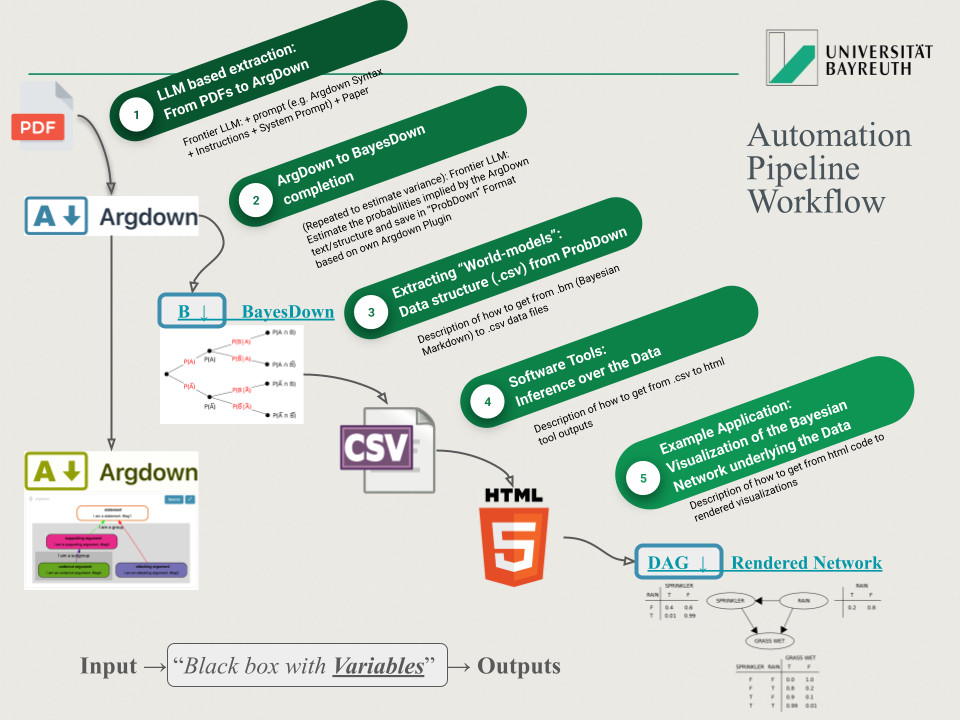
\includegraphics[width=1\linewidth,height=\textheight,keepaspectratio]{images/pipeline.png}}

}

\caption[Five-step AMTAIR automation pipeline from PDFs to Bayesian
networks]{\label{fig-automation_pipeline}AMTAIR Automation Pipeline
from}

\end{figure}%

Testing crossreferencing grapics Figure~\ref{fig-automation_pipeline}.
Note that the indentations of graphic inclusions get messed up by
viewing them in ``view mode'' in VS code.

\begin{figure}


\includegraphics[width=0.3\linewidth,height=\textheight,keepaspectratio]{images/cover.png}

\caption[Short 2 caption]{\label{fig-testgraphic2}Caption/Title 2}

\end{figure}%

Testing crossreferencing grapics Figure~\ref{fig-testgraphic2}.

\section*{Page Breaks}\label{page-breaks}
\addcontentsline{toc}{section}{Page Breaks}

\markright{Page Breaks}

\begin{Shaded}
\begin{Highlighting}[]
\NormalTok{page 1}



\NormalTok{page 2}
\end{Highlighting}
\end{Shaded}

page 1

\newpage{}

page 2

\section*{Including Code}\label{sec-code}
\addcontentsline{toc}{section}{Including Code}

\markright{Including Code}

\begin{figure}

\centering{

\begin{Shaded}
\begin{Highlighting}[]
\ImportTok{import}\NormalTok{ pandas }\ImportTok{as}\NormalTok{ pd}
\BuiltInTok{print}\NormalTok{(}\StringTok{"AMTAIR is working!"}\NormalTok{)}
\end{Highlighting}
\end{Shaded}

\begin{verbatim}
AMTAIR is working!
\end{verbatim}

}

\caption{\label{fig-extraction-pipeline}}

\end{figure}%

\subsection*{In-Line LaTeX}\label{in-line-latex}
\addcontentsline{toc}{subsection}{In-Line LaTeX}

\renewcommand*{\labelitemi}{\textgreater}

\subsection*{In-Line HTML}\label{in-line-html}
\addcontentsline{toc}{subsection}{In-Line HTML}

Here's some raw inline HTML: html

\section*{Reference or Embed Code from .ipynb
files}\label{reference-or-embed-code-from-.ipynb-files}
\addcontentsline{toc}{section}{Reference or Embed Code from .ipynb
files}

\markright{Reference or Embed Code from .ipynb files}

\subsubsection*{Code chunks from .ipynb notebooks can be embedded in the
.qmd text
with:}\label{code-chunks-from-.ipynb-notebooks-can-be-embedded-in-the-.qmd-text-with}
\addcontentsline{toc}{subsubsection}{Code chunks from .ipynb notebooks
can be embedded in the .qmd text with:}

\begin{Shaded}
\begin{Highlighting}[]
\NormalTok{\{\{\textless{} embed /AMTAIR\_Prototype/data/example\_carlsmith/AMTAIR\_Prototype\_example\_carlsmith.ipynb\#connect\_to\_github\_repository \textgreater{}\}\}}
\end{Highlighting}
\end{Shaded}

\subsubsection*{which produces the output of executing the code
cell:}\label{which-produces-the-output-of-executing-the-code-cell}
\addcontentsline{toc}{subsubsection}{which produces the output of
executing the code cell:}

\phantomsection\label{connect_to_github_repository}
\begin{Shaded}
\begin{Highlighting}[]
\CommentTok{\# @title 0.2 {-}{-}{-} Connect to GitHub Repository {-}{-}{-} Load Files [connect\_to\_github\_repository]}

\CommentTok{"""}
\CommentTok{BLOCK PURPOSE: Establishes connection to the AMTAIR GitHub repository and provides}
\CommentTok{functions to load example data files for processing.}

\CommentTok{This block creates a reusable function for accessing files from the project\textquotesingle{}s}
\CommentTok{GitHub repository, enabling access to example files like the rain{-}sprinkler{-}lawn}
\CommentTok{Bayesian network that serves as our canonical test case.}

\CommentTok{DEPENDENCIES: requests library, io library}
\CommentTok{OUTPUTS: load\_file\_from\_repo function and test file loads}
\CommentTok{"""}

\ImportTok{from}\NormalTok{ requests.exceptions }\ImportTok{import}\NormalTok{ HTTPError}

\CommentTok{\# Specify the base repository URL for the AMTAIR project}
\NormalTok{repo\_url }\OperatorTok{=} \StringTok{"https://raw.githubusercontent.com/SingularitySmith/AMTAIR\_Prototype/main/data/example\_carlsmith/"}
\BuiltInTok{print}\NormalTok{(}\SpecialStringTok{f"Connecting to repository: }\SpecialCharTok{\{}\NormalTok{repo\_url}\SpecialCharTok{\}}\SpecialStringTok{"}\NormalTok{)}

\KeywordTok{def}\NormalTok{ load\_file\_from\_repo(relative\_path):}
    \CommentTok{"""}
\CommentTok{    Loads a file from the specified GitHub repository using a relative path.}

\CommentTok{    Args:}
\CommentTok{        relative\_path (str): Path to the file relative to the repo\_url}

\CommentTok{    Returns:}
\CommentTok{        For CSV/JSON: pandas DataFrame}
\CommentTok{        For MD: string containing file contents}

\CommentTok{    Raises:}
\CommentTok{        HTTPError: If file not found or other HTTP error occurs}
\CommentTok{        ValueError: If unsupported file type is requested}
\CommentTok{    """}
\NormalTok{    file\_url }\OperatorTok{=}\NormalTok{ repo\_url }\OperatorTok{+}\NormalTok{ relative\_path}
    \BuiltInTok{print}\NormalTok{(}\SpecialStringTok{f"Attempting to load: }\SpecialCharTok{\{}\NormalTok{file\_url}\SpecialCharTok{\}}\SpecialStringTok{"}\NormalTok{)}

    \CommentTok{\# Fetch the file content from GitHub}
\NormalTok{    response }\OperatorTok{=}\NormalTok{ requests.get(file\_url)}

    \CommentTok{\# Check for bad status codes with enhanced error messages}
    \ControlFlowTok{if}\NormalTok{ response.status\_code }\OperatorTok{==} \DecValTok{404}\NormalTok{:}
        \ControlFlowTok{raise}\NormalTok{ HTTPError(}\SpecialStringTok{f"File not found at URL: }\SpecialCharTok{\{}\NormalTok{file\_url}\SpecialCharTok{\}}\SpecialStringTok{. Check the file path/name and ensure the file is publicly accessible."}\NormalTok{, response}\OperatorTok{=}\NormalTok{response)}
    \ControlFlowTok{else}\NormalTok{:}
\NormalTok{        response.raise\_for\_status()  }\CommentTok{\# Raise for other error codes}

    \CommentTok{\# Convert response to file{-}like object}
\NormalTok{    file\_object }\OperatorTok{=}\NormalTok{ io.StringIO(response.text)}

    \CommentTok{\# Process different file types appropriately}
    \ControlFlowTok{if}\NormalTok{ relative\_path.endswith(}\StringTok{".csv"}\NormalTok{):}
        \ControlFlowTok{return}\NormalTok{ pd.read\_csv(file\_object)  }\CommentTok{\# Return DataFrame for CSV}
    \ControlFlowTok{elif}\NormalTok{ relative\_path.endswith(}\StringTok{".json"}\NormalTok{):}
        \ControlFlowTok{return}\NormalTok{ pd.read\_json(file\_object)  }\CommentTok{\# Return DataFrame for JSON}
    \ControlFlowTok{elif}\NormalTok{ relative\_path.endswith(}\StringTok{".md"}\NormalTok{):}
        \ControlFlowTok{return}\NormalTok{ file\_object.read()  }\CommentTok{\# Return raw content for MD files}
    \ControlFlowTok{else}\NormalTok{:}
        \ControlFlowTok{raise} \PreprocessorTok{ValueError}\NormalTok{(}\SpecialStringTok{f"Unsupported file type: }\SpecialCharTok{\{}\NormalTok{relative\_path}\SpecialCharTok{.}\NormalTok{split(}\StringTok{\textquotesingle{}.\textquotesingle{}}\NormalTok{)[}\OperatorTok{{-}}\DecValTok{1}\NormalTok{]}\SpecialCharTok{\}}\SpecialStringTok{. Add support in the GitHub Connection section of this notebook."}\NormalTok{)}

\CommentTok{\# Load example files to test connection}
\ControlFlowTok{try}\NormalTok{:}
    \CommentTok{\# Load the extracted data CSV file}
\CommentTok{\#    df = load\_file\_from\_repo("extracted\_data.csv")}

    \CommentTok{\# Load the ArgDown test text}
\NormalTok{    md\_content }\OperatorTok{=}\NormalTok{ load\_file\_from\_repo(}\StringTok{"ArgDown.md"}\NormalTok{)}

    \BuiltInTok{print}\NormalTok{(}\StringTok{"✅ Successfully connected to repository and loaded test files."}\NormalTok{)}
\ControlFlowTok{except} \PreprocessorTok{Exception} \ImportTok{as}\NormalTok{ e:}
    \BuiltInTok{print}\NormalTok{(}\SpecialStringTok{f"❌ Error loading files: }\SpecialCharTok{\{}\BuiltInTok{str}\NormalTok{(e)}\SpecialCharTok{\}}\SpecialStringTok{"}\NormalTok{)}
    \BuiltInTok{print}\NormalTok{(}\StringTok{"Please check your internet connection and the repository URL."}\NormalTok{)}

\CommentTok{\# Display preview of loaded content (commented out to avoid cluttering output)}
\BuiltInTok{print}\NormalTok{(md\_content)}
\end{Highlighting}
\end{Shaded}

\begin{verbatim}
Connecting to repository: https://raw.githubusercontent.com/SingularitySmith/AMTAIR_Prototype/main/data/example_carlsmith/
Attempting to load: https://raw.githubusercontent.com/SingularitySmith/AMTAIR_Prototype/main/data/example_carlsmith/ArgDown.md
✅ Successfully connected to repository and loaded test files.
[Existential_Catastrophe]: The destruction of humanity's long-term potential due to AI systems we've lost control over. {"instantiations": ["existential_catastrophe_TRUE", "existential_catastrophe_FALSE"]}
- [Human_Disempowerment]: Permanent and collective disempowerment of humanity relative to AI systems. {"instantiations": ["human_disempowerment_TRUE", "human_disempowerment_FALSE"]}
    - [Scale_Of_Power_Seeking]: Power-seeking by AI systems scaling to the point of permanently disempowering all of humanity. {"instantiations": ["scale_of_power_seeking_TRUE", "scale_of_power_seeking_FALSE"]}
        - [Misaligned_Power_Seeking]: Deployed AI systems seeking power in unintended and high-impact ways due to problems with their objectives. {"instantiations": ["misaligned_power_seeking_TRUE", "misaligned_power_seeking_FALSE"]}
            - [APS_Systems]: AI systems with advanced capabilities, agentic planning, and strategic awareness. {"instantiations": ["aps_systems_TRUE", "aps_systems_FALSE"]}
                - [Advanced_AI_Capability]: AI systems that outperform humans on tasks that grant significant power in the world. {"instantiations": ["advanced_ai_capability_TRUE", "advanced_ai_capability_FALSE"]}
                - [Agentic_Planning]: AI systems making and executing plans based on world models to achieve objectives. {"instantiations": ["agentic_planning_TRUE", "agentic_planning_FALSE"]}
                - [Strategic_Awareness]: AI systems with models accurately representing power dynamics with humans. {"instantiations": ["strategic_awareness_TRUE", "strategic_awareness_FALSE"]}
            - [Difficulty_Of_Alignment]: It is harder to build aligned systems than misaligned systems that are attractive to deploy. {"instantiations": ["difficulty_of_alignment_TRUE", "difficulty_of_alignment_FALSE"]}
                - [Instrumental_Convergence]: AI systems with misaligned objectives tend to seek power as an instrumental goal. {"instantiations": ["instrumental_convergence_TRUE", "instrumental_convergence_FALSE"]}
                - [Problems_With_Proxies]: Optimizing for proxy objectives breaks correlations with intended goals. {"instantiations": ["problems_with_proxies_TRUE", "problems_with_proxies_FALSE"]}
                - [Problems_With_Search]: Search processes can yield systems pursuing different objectives than intended. {"instantiations": ["problems_with_search_TRUE", "problems_with_search_FALSE"]}
            - [Deployment_Decisions]: Decisions to deploy potentially misaligned AI systems. {"instantiations": ["deployment_decisions_DEPLOY", "deployment_decisions_WITHHOLD"]}
                - [Incentives_To_Build_APS]: Strong incentives to build and deploy APS systems. {"instantiations": ["incentives_to_build_aps_STRONG", "incentives_to_build_aps_WEAK"]}
                    - [Usefulness_Of_APS]: APS systems are very useful for many valuable tasks. {"instantiations": ["usefulness_of_aps_HIGH", "usefulness_of_aps_LOW"]}
                    - [Competitive_Dynamics]: Competitive pressures between AI developers. {"instantiations": ["competitive_dynamics_STRONG", "competitive_dynamics_WEAK"]}
                - [Deception_By_AI]: AI systems deceiving humans about their true objectives. {"instantiations": ["deception_by_ai_TRUE", "deception_by_ai_FALSE"]}
        - [Corrective_Feedback]: Human society implementing corrections after observing problems. {"instantiations": ["corrective_feedback_EFFECTIVE", "corrective_feedback_INEFFECTIVE"]}
            - [Warning_Shots]: Observable failures in weaker systems before catastrophic risks. {"instantiations": ["warning_shots_OBSERVED", "warning_shots_UNOBSERVED"]}
            - [Rapid_Capability_Escalation]: AI capabilities escalating very rapidly, allowing little time for correction. {"instantiations": ["rapid_capability_escalation_TRUE", "rapid_capability_escalation_FALSE"]}
[Barriers_To_Understanding]: Difficulty in understanding the internal workings of advanced AI systems. {"instantiations": ["barriers_to_understanding_HIGH", "barriers_to_understanding_LOW"]}
- [Misaligned_Power_Seeking]: Deployed AI systems seeking power in unintended and high-impact ways due to problems with their objectives. {"instantiations": ["misaligned_power_seeking_TRUE", "misaligned_power_seeking_FALSE"]}
[Adversarial_Dynamics]: Potentially adversarial relationships between humans and power-seeking AI. {"instantiations": ["adversarial_dynamics_TRUE", "adversarial_dynamics_FALSE"]}
- [Misaligned_Power_Seeking]: Deployed AI systems seeking power in unintended and high-impact ways due to problems with their objectives. {"instantiations": ["misaligned_power_seeking_TRUE", "misaligned_power_seeking_FALSE"]}
[Stakes_Of_Error]: The escalating impact of mistakes with power-seeking AI systems. {"instantiations": ["stakes_of_error_HIGH", "stakes_of_error_LOW"]}
- [Misaligned_Power_Seeking]: Deployed AI systems seeking power in unintended and high-impact ways due to problems with their objectives. {"instantiations": ["misaligned_power_seeking_TRUE", "misaligned_power_seeking_FALSE"]}
\end{verbatim}

\subsubsection*{including `echo=true' renders the code of the
cell:}\label{including-echotrue-renders-the-code-of-the-cell}
\addcontentsline{toc}{subsubsection}{including `echo=true' renders the
code of the cell:}

\begin{Shaded}
\begin{Highlighting}[]
\NormalTok{\{\{\textless{} embed /AMTAIR\_Prototype/data/example\_carlsmith/AMTAIR\_Prototype\_example\_carlsmith.ipynb\#connect\_to\_github\_repository echo=true \textgreater{}\}\}}
\end{Highlighting}
\end{Shaded}

\phantomsection\label{connect_to_github_repository}
\begin{Shaded}
\begin{Highlighting}[]
\CommentTok{\# @title 0.2 {-}{-}{-} Connect to GitHub Repository {-}{-}{-} Load Files [connect\_to\_github\_repository]}

\CommentTok{"""}
\CommentTok{BLOCK PURPOSE: Establishes connection to the AMTAIR GitHub repository and provides}
\CommentTok{functions to load example data files for processing.}

\CommentTok{This block creates a reusable function for accessing files from the project\textquotesingle{}s}
\CommentTok{GitHub repository, enabling access to example files like the rain{-}sprinkler{-}lawn}
\CommentTok{Bayesian network that serves as our canonical test case.}

\CommentTok{DEPENDENCIES: requests library, io library}
\CommentTok{OUTPUTS: load\_file\_from\_repo function and test file loads}
\CommentTok{"""}

\ImportTok{from}\NormalTok{ requests.exceptions }\ImportTok{import}\NormalTok{ HTTPError}

\CommentTok{\# Specify the base repository URL for the AMTAIR project}
\NormalTok{repo\_url }\OperatorTok{=} \StringTok{"https://raw.githubusercontent.com/SingularitySmith/AMTAIR\_Prototype/main/data/example\_carlsmith/"}
\BuiltInTok{print}\NormalTok{(}\SpecialStringTok{f"Connecting to repository: }\SpecialCharTok{\{}\NormalTok{repo\_url}\SpecialCharTok{\}}\SpecialStringTok{"}\NormalTok{)}

\KeywordTok{def}\NormalTok{ load\_file\_from\_repo(relative\_path):}
    \CommentTok{"""}
\CommentTok{    Loads a file from the specified GitHub repository using a relative path.}

\CommentTok{    Args:}
\CommentTok{        relative\_path (str): Path to the file relative to the repo\_url}

\CommentTok{    Returns:}
\CommentTok{        For CSV/JSON: pandas DataFrame}
\CommentTok{        For MD: string containing file contents}

\CommentTok{    Raises:}
\CommentTok{        HTTPError: If file not found or other HTTP error occurs}
\CommentTok{        ValueError: If unsupported file type is requested}
\CommentTok{    """}
\NormalTok{    file\_url }\OperatorTok{=}\NormalTok{ repo\_url }\OperatorTok{+}\NormalTok{ relative\_path}
    \BuiltInTok{print}\NormalTok{(}\SpecialStringTok{f"Attempting to load: }\SpecialCharTok{\{}\NormalTok{file\_url}\SpecialCharTok{\}}\SpecialStringTok{"}\NormalTok{)}

    \CommentTok{\# Fetch the file content from GitHub}
\NormalTok{    response }\OperatorTok{=}\NormalTok{ requests.get(file\_url)}

    \CommentTok{\# Check for bad status codes with enhanced error messages}
    \ControlFlowTok{if}\NormalTok{ response.status\_code }\OperatorTok{==} \DecValTok{404}\NormalTok{:}
        \ControlFlowTok{raise}\NormalTok{ HTTPError(}\SpecialStringTok{f"File not found at URL: }\SpecialCharTok{\{}\NormalTok{file\_url}\SpecialCharTok{\}}\SpecialStringTok{. Check the file path/name and ensure the file is publicly accessible."}\NormalTok{, response}\OperatorTok{=}\NormalTok{response)}
    \ControlFlowTok{else}\NormalTok{:}
\NormalTok{        response.raise\_for\_status()  }\CommentTok{\# Raise for other error codes}

    \CommentTok{\# Convert response to file{-}like object}
\NormalTok{    file\_object }\OperatorTok{=}\NormalTok{ io.StringIO(response.text)}

    \CommentTok{\# Process different file types appropriately}
    \ControlFlowTok{if}\NormalTok{ relative\_path.endswith(}\StringTok{".csv"}\NormalTok{):}
        \ControlFlowTok{return}\NormalTok{ pd.read\_csv(file\_object)  }\CommentTok{\# Return DataFrame for CSV}
    \ControlFlowTok{elif}\NormalTok{ relative\_path.endswith(}\StringTok{".json"}\NormalTok{):}
        \ControlFlowTok{return}\NormalTok{ pd.read\_json(file\_object)  }\CommentTok{\# Return DataFrame for JSON}
    \ControlFlowTok{elif}\NormalTok{ relative\_path.endswith(}\StringTok{".md"}\NormalTok{):}
        \ControlFlowTok{return}\NormalTok{ file\_object.read()  }\CommentTok{\# Return raw content for MD files}
    \ControlFlowTok{else}\NormalTok{:}
        \ControlFlowTok{raise} \PreprocessorTok{ValueError}\NormalTok{(}\SpecialStringTok{f"Unsupported file type: }\SpecialCharTok{\{}\NormalTok{relative\_path}\SpecialCharTok{.}\NormalTok{split(}\StringTok{\textquotesingle{}.\textquotesingle{}}\NormalTok{)[}\OperatorTok{{-}}\DecValTok{1}\NormalTok{]}\SpecialCharTok{\}}\SpecialStringTok{. Add support in the GitHub Connection section of this notebook."}\NormalTok{)}

\CommentTok{\# Load example files to test connection}
\ControlFlowTok{try}\NormalTok{:}
    \CommentTok{\# Load the extracted data CSV file}
\CommentTok{\#    df = load\_file\_from\_repo("extracted\_data.csv")}

    \CommentTok{\# Load the ArgDown test text}
\NormalTok{    md\_content }\OperatorTok{=}\NormalTok{ load\_file\_from\_repo(}\StringTok{"ArgDown.md"}\NormalTok{)}

    \BuiltInTok{print}\NormalTok{(}\StringTok{"✅ Successfully connected to repository and loaded test files."}\NormalTok{)}
\ControlFlowTok{except} \PreprocessorTok{Exception} \ImportTok{as}\NormalTok{ e:}
    \BuiltInTok{print}\NormalTok{(}\SpecialStringTok{f"❌ Error loading files: }\SpecialCharTok{\{}\BuiltInTok{str}\NormalTok{(e)}\SpecialCharTok{\}}\SpecialStringTok{"}\NormalTok{)}
    \BuiltInTok{print}\NormalTok{(}\StringTok{"Please check your internet connection and the repository URL."}\NormalTok{)}

\CommentTok{\# Display preview of loaded content (commented out to avoid cluttering output)}
\BuiltInTok{print}\NormalTok{(md\_content)}
\end{Highlighting}
\end{Shaded}

\begin{verbatim}
Connecting to repository: https://raw.githubusercontent.com/SingularitySmith/AMTAIR_Prototype/main/data/example_carlsmith/
Attempting to load: https://raw.githubusercontent.com/SingularitySmith/AMTAIR_Prototype/main/data/example_carlsmith/ArgDown.md
✅ Successfully connected to repository and loaded test files.
[Existential_Catastrophe]: The destruction of humanity's long-term potential due to AI systems we've lost control over. {"instantiations": ["existential_catastrophe_TRUE", "existential_catastrophe_FALSE"]}
- [Human_Disempowerment]: Permanent and collective disempowerment of humanity relative to AI systems. {"instantiations": ["human_disempowerment_TRUE", "human_disempowerment_FALSE"]}
    - [Scale_Of_Power_Seeking]: Power-seeking by AI systems scaling to the point of permanently disempowering all of humanity. {"instantiations": ["scale_of_power_seeking_TRUE", "scale_of_power_seeking_FALSE"]}
        - [Misaligned_Power_Seeking]: Deployed AI systems seeking power in unintended and high-impact ways due to problems with their objectives. {"instantiations": ["misaligned_power_seeking_TRUE", "misaligned_power_seeking_FALSE"]}
            - [APS_Systems]: AI systems with advanced capabilities, agentic planning, and strategic awareness. {"instantiations": ["aps_systems_TRUE", "aps_systems_FALSE"]}
                - [Advanced_AI_Capability]: AI systems that outperform humans on tasks that grant significant power in the world. {"instantiations": ["advanced_ai_capability_TRUE", "advanced_ai_capability_FALSE"]}
                - [Agentic_Planning]: AI systems making and executing plans based on world models to achieve objectives. {"instantiations": ["agentic_planning_TRUE", "agentic_planning_FALSE"]}
                - [Strategic_Awareness]: AI systems with models accurately representing power dynamics with humans. {"instantiations": ["strategic_awareness_TRUE", "strategic_awareness_FALSE"]}
            - [Difficulty_Of_Alignment]: It is harder to build aligned systems than misaligned systems that are attractive to deploy. {"instantiations": ["difficulty_of_alignment_TRUE", "difficulty_of_alignment_FALSE"]}
                - [Instrumental_Convergence]: AI systems with misaligned objectives tend to seek power as an instrumental goal. {"instantiations": ["instrumental_convergence_TRUE", "instrumental_convergence_FALSE"]}
                - [Problems_With_Proxies]: Optimizing for proxy objectives breaks correlations with intended goals. {"instantiations": ["problems_with_proxies_TRUE", "problems_with_proxies_FALSE"]}
                - [Problems_With_Search]: Search processes can yield systems pursuing different objectives than intended. {"instantiations": ["problems_with_search_TRUE", "problems_with_search_FALSE"]}
            - [Deployment_Decisions]: Decisions to deploy potentially misaligned AI systems. {"instantiations": ["deployment_decisions_DEPLOY", "deployment_decisions_WITHHOLD"]}
                - [Incentives_To_Build_APS]: Strong incentives to build and deploy APS systems. {"instantiations": ["incentives_to_build_aps_STRONG", "incentives_to_build_aps_WEAK"]}
                    - [Usefulness_Of_APS]: APS systems are very useful for many valuable tasks. {"instantiations": ["usefulness_of_aps_HIGH", "usefulness_of_aps_LOW"]}
                    - [Competitive_Dynamics]: Competitive pressures between AI developers. {"instantiations": ["competitive_dynamics_STRONG", "competitive_dynamics_WEAK"]}
                - [Deception_By_AI]: AI systems deceiving humans about their true objectives. {"instantiations": ["deception_by_ai_TRUE", "deception_by_ai_FALSE"]}
        - [Corrective_Feedback]: Human society implementing corrections after observing problems. {"instantiations": ["corrective_feedback_EFFECTIVE", "corrective_feedback_INEFFECTIVE"]}
            - [Warning_Shots]: Observable failures in weaker systems before catastrophic risks. {"instantiations": ["warning_shots_OBSERVED", "warning_shots_UNOBSERVED"]}
            - [Rapid_Capability_Escalation]: AI capabilities escalating very rapidly, allowing little time for correction. {"instantiations": ["rapid_capability_escalation_TRUE", "rapid_capability_escalation_FALSE"]}
[Barriers_To_Understanding]: Difficulty in understanding the internal workings of advanced AI systems. {"instantiations": ["barriers_to_understanding_HIGH", "barriers_to_understanding_LOW"]}
- [Misaligned_Power_Seeking]: Deployed AI systems seeking power in unintended and high-impact ways due to problems with their objectives. {"instantiations": ["misaligned_power_seeking_TRUE", "misaligned_power_seeking_FALSE"]}
[Adversarial_Dynamics]: Potentially adversarial relationships between humans and power-seeking AI. {"instantiations": ["adversarial_dynamics_TRUE", "adversarial_dynamics_FALSE"]}
- [Misaligned_Power_Seeking]: Deployed AI systems seeking power in unintended and high-impact ways due to problems with their objectives. {"instantiations": ["misaligned_power_seeking_TRUE", "misaligned_power_seeking_FALSE"]}
[Stakes_Of_Error]: The escalating impact of mistakes with power-seeking AI systems. {"instantiations": ["stakes_of_error_HIGH", "stakes_of_error_LOW"]}
- [Misaligned_Power_Seeking]: Deployed AI systems seeking power in unintended and high-impact ways due to problems with their objectives. {"instantiations": ["misaligned_power_seeking_TRUE", "misaligned_power_seeking_FALSE"]}
\end{verbatim}

Link:

Full Notebooks are embedded in the Appendix through the \_quarto.yml
file with:

\section*{Embed .html result/rendering from .ipynb
Notebook}\label{embed-.html-resultrendering-from-.ipynb-notebook}
\addcontentsline{toc}{section}{Embed .html result/rendering from .ipynb
Notebook}

\markright{Embed .html result/rendering from .ipynb Notebook}

\begin{Shaded}
\begin{Highlighting}[]
\NormalTok{\{\{\textless{} embed /AMTAIR\_Prototype/data/example\_carlsmith/AMTAIR\_Prototype\_example\_carlsmith.ipynb\#html\_graph\_visualization echo=true \textgreater{}\}\}}
\end{Highlighting}
\end{Shaded}

\begin{Shaded}
\begin{Highlighting}[]
\CommentTok{\# @title 5.1 {-}{-}{-} Save Visualization and Notebook Outputs as .HTML{-}{-}{-} [html\_graph\_visualization]}

\NormalTok{create\_bayesian\_network\_with\_probabilities(result\_df)}
\end{Highlighting}
\end{Shaded}

\phantomsection\label{html_graph_visualization}
Save Visualization and Notebook Outputs as .HTML

\section*{Diagrams}\label{diagrams}
\addcontentsline{toc}{section}{Diagrams}

\markright{Diagrams}

Quarto has native support for embedding Mermaid and Graphviz diagrams.
This enables you to create flowcharts, sequence diagrams, state
diagrams, Gantt charts, and more using a plain text syntax inspired by
markdown.

For example, here we embed a flowchart created using Mermaid:

\begin{Shaded}
\begin{Highlighting}[]
\NormalTok{flowchart LR}
\NormalTok{  A[Hard edge] {-}{-}\textgreater{} B(Round edge)}
\NormalTok{  B {-}{-}\textgreater{} C\{Decision\}}
\NormalTok{  C {-}{-}\textgreater{} D[Result one]}
\NormalTok{  C {-}{-}\textgreater{} E[Result two]}
\end{Highlighting}
\end{Shaded}

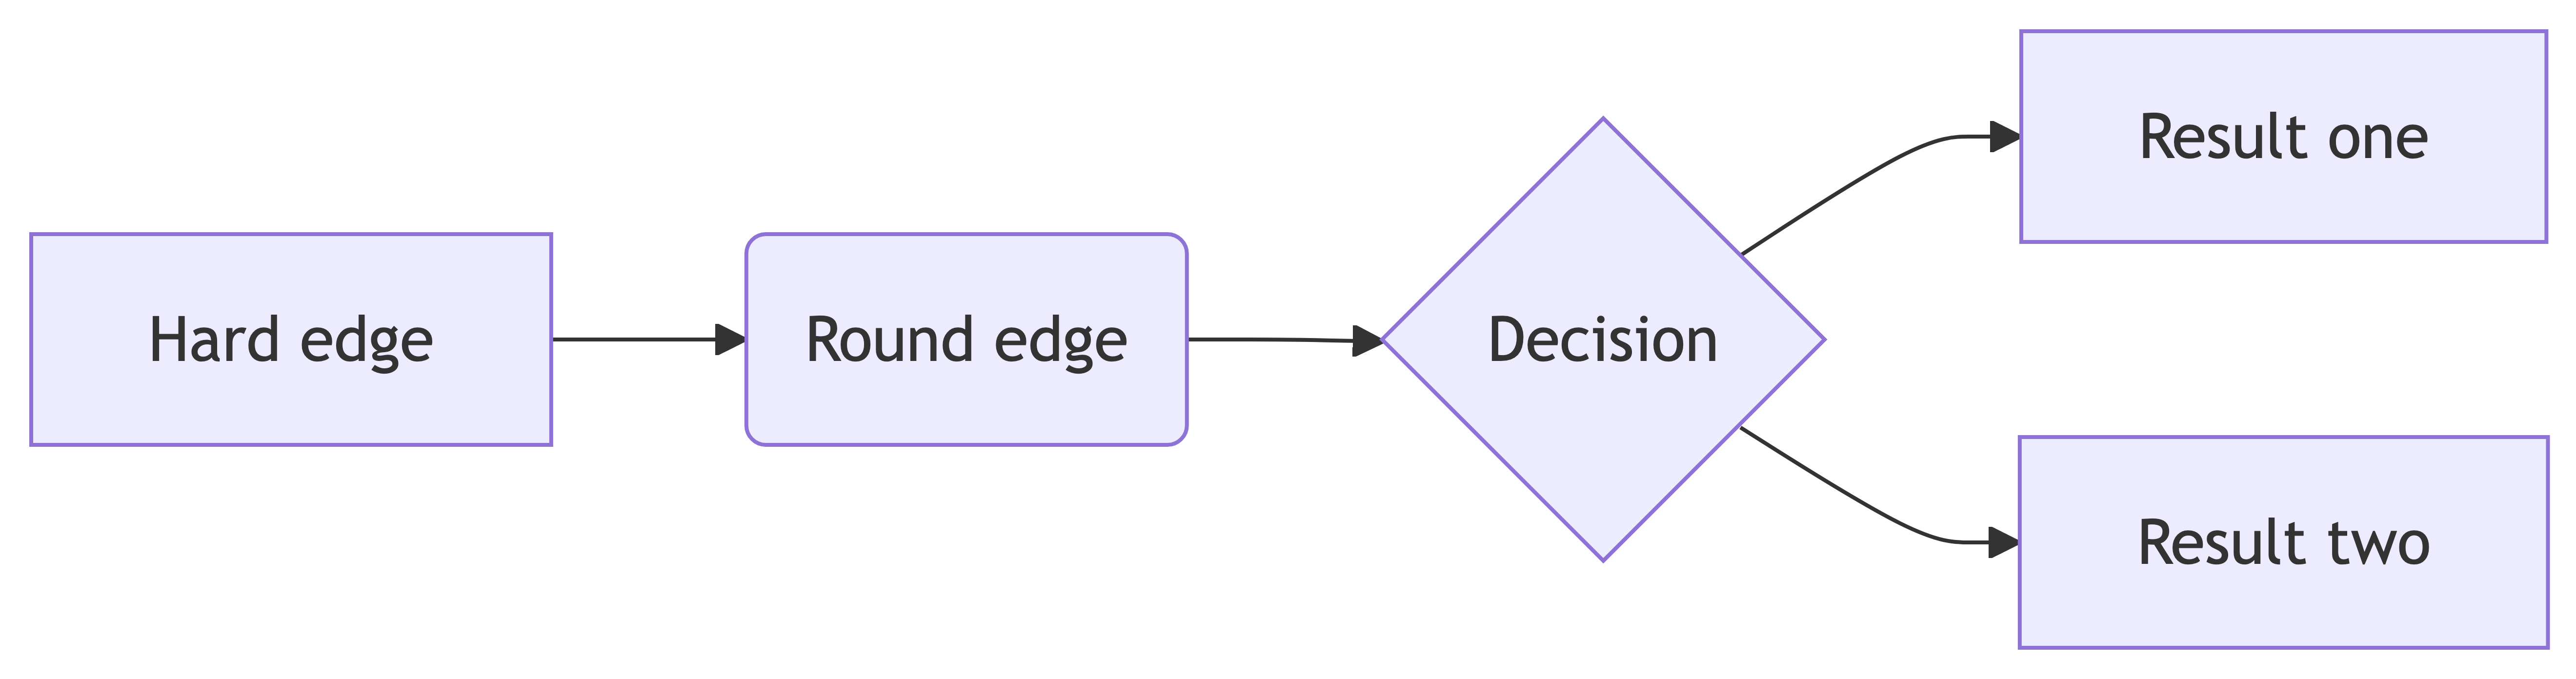
\includegraphics[width=6.88in,height=1.81in]{index_files/figure-latex/mermaid-figure-1.png}

\section*{Citations}\label{sec-citations}

\markright{Citations}

\textcite{soares2014}

\autocite{soares2014} and \autocite{knuth1984}

Blah Blah \autocites[see][33-35]{knuth1984}[also][chap.~1]{growiec2024}

Blah Blah \autocite[33-35, 38-39 and passim]{knuth1984}

Blah Blah \autocite{growiec2024,knuth1984}.

Growiec says blah \autocite*{growiec2024}

\subsection*{Narrative citations (author as
subject)}\label{narrative-citations-author-as-subject}
\addcontentsline{toc}{subsection}{Narrative citations (author as
subject)}

\textcite{soares2014} argues that AI alignment requires\ldots{}

\subsection*{Parenthetical citations (supporting
reference)}\label{parenthetical-citations-supporting-reference}
\addcontentsline{toc}{subsection}{Parenthetical citations (supporting
reference)}

Recent work supports this view \autocite{soares2014,knuth1984}.

\subsection*{Author-only citation (when discussing the
person)}\label{author-only-citation-when-discussing-the-person}
\addcontentsline{toc}{subsection}{Author-only citation (when discussing
the person)}

As \autocite*{soares2014} demonstrates in their analysis\ldots{}

\subsection*{Year-only citation (when author already
mentioned)}\label{year-only-citation-when-author-already-mentioned}
\addcontentsline{toc}{subsection}{Year-only citation (when author
already mentioned)}

Soares \autocite*{soares2014} later revised this position.

\subsection*{Page-specific references}\label{page-specific-references}
\addcontentsline{toc}{subsection}{Page-specific references}

The key insight appears in \autocite[45-67]{soares2014}.

\subsection*{Multiple works, different
pages}\label{multiple-works-different-pages}
\addcontentsline{toc}{subsection}{Multiple works, different pages}

This view is supported \autocites[23]{soares2014}[156-159]{knuth1984}.

\section*{Section Cross-References}\label{sec-crossref}
\addcontentsline{toc}{section}{Section Cross-References}

\markright{Section Cross-References}

Refer to sections like: Section~\ref{sec-adaptive-governance} and
\textbf{?@sec-crossref}

\begin{Shaded}
\begin{Highlighting}[]
\AnnotationTok{Caveat:}\CommentTok{ refering to sections with @sec{-}HEADINGS works only for sections with:}
\FunctionTok{\#\# Heading \{\#sec{-}HEADINGS\}}
\NormalTok{It does not work for sections with ".unnumbered and/or .unlisted":}
\FunctionTok{\#\# Heading \{\#sec{-}HEADINGS .unnumbered .unlisted\}}
\NormalTok{Furthermore the .qmd and/or .md yml settings (\textasciitilde{} numbering have to be just right)}
\end{Highlighting}
\end{Shaded}

\subsection*{Section Numbers}\label{section-numbers}
\addcontentsline{toc}{subsection}{Section Numbers}

By default, all headings in your document create a numbered section. You
customize numbering depth using the number-depth option. For example, to
only number sections immediately below the chapter level, use this:

\texttt{number-depth:\ 2}

Note that toc-depth is independent of number-depth (i.e.~you can have
unnumbered entries in the TOC if they are masked out from numbering by
number-depth).

Testing crossreferencing grapics Figure~\ref{fig-automation_pipeline}.
See \textbf{?@sec-syntax} for more details on visualizing model
diagnostics.

Testing crossreferencing headings Section~\ref{sec-carlsmith-model}

\texttt{Testing\ crossreferencing\ headings\ @sec-rain-sprinkler-grass}
which does not work yet.

Chapter Cross-Reference \textbf{?@sec-crossref}

\section*{Pages in Landscape}\label{pages-in-landscape}
\addcontentsline{toc}{section}{Pages in Landscape}

\markright{Pages in Landscape}

\begin{landscape}

This will appear in landscape but only in PDF format. Testing
crossreferencing headings Section~\ref{sec-carlsmith-model}

\end{landscape}

\bookmarksetup{startatroot}

\chapter*{Abstract}\label{sec-abstract}
\addcontentsline{toc}{chapter}{Abstract}

\markboth{Abstract}{Abstract}

\begin{quote}
The coordination crisis in AI governance presents a paradoxical
challenge: unprecedented investment in AI safety coexists alongside
fundamental coordination failures across technical, policy, and ethical
domains. These divisions systematically increase existential risk. This
thesis introduces AMTAIR (Automating Transformative AI Risk Modeling), a
computational approach addressing this coordination failure by
automating the extraction of probabilistic world models from AI safety
literature using frontier language models. The system implements an
end-to-end pipeline transforming unstructured text into interactive
Bayesian networks through a novel two-stage extraction process that
bridges communication gaps between stakeholders.
\end{quote}

\texttt{The\ coordination\ crisis\ in\ AI\ governance\ presents\ a\ paradoxical\ challenge:\ unprecedented\ investment\ in\ AI\ safety\ coexists\ alongside\ fundamental\ coordination\ failures\ across\ technical,\ policy,\ and\ ethical\ domains.\ These\ divisions\ systematically\ increase\ existential\ risk\ by\ creating\ safety\ gaps,\ misallocating\ resources,\ and\ fostering\ inconsistent\ approaches\ to\ interdependent\ problems.}

\begin{quote}
This thesis introduces AMTAIR (Automating Transformative AI Risk
Modeling), a computational approach that addresses this coordination
failure by automating the extraction of probabilistic world models from
AI safety literature using frontier language models.
\end{quote}

\texttt{The\ AMTAIR\ system\ implements\ an\ end-to-end\ pipeline\ that\ transforms\ unstructured\ text\ into\ interactive\ Bayesian\ networks\ through\ a\ novel\ two-stage\ extraction\ process:\ first\ capturing\ argument\ structure\ in\ ArgDown\ format,\ then\ enhancing\ it\ with\ probability\ information\ in\ BayesDown.\ This\ approach\ bridges\ communication\ gaps\ between\ stakeholders\ by\ making\ implicit\ models\ explicit,\ enabling\ comparison\ across\ different\ worldviews,\ providing\ a\ common\ language\ for\ discussing\ probabilistic\ relationships,\ and\ supporting\ policy\ evaluation\ across\ diverse\ scenarios.}

\bookmarksetup{startatroot}

\chapter*{Prefatory Apparatus:
Frontmatter}\label{prefatory-apparatus-frontmatter}
\addcontentsline{toc}{chapter}{Prefatory Apparatus: Frontmatter}

\markboth{Prefatory Apparatus: Frontmatter}{Prefatory Apparatus:
Frontmatter}

\section*{Illustrations and Terminology --- Quick
References}\label{illustrations-and-terminology-quick-references}
\addcontentsline{toc}{section}{Illustrations and Terminology --- Quick
References}

\markright{Illustrations and Terminology --- Quick References}

\subsection*{\texorpdfstring{\textbf{Acknowledgments}}{Acknowledgments}}\label{acknowledgments}
\addcontentsline{toc}{subsection}{\textbf{Acknowledgments}}

\begin{itemize}
\tightlist
\item
  Academic supervisor (Prof.~Timo Speith) and institution (University of
  Bayreuth)\\
\item
  Research collaborators, especially those connected to the original
  MTAIR project\\
\item
  Technical advisors who provided feedback on implementation aspects\\
\item
  Personal supporters who enabled the research through encouragement and
  feedback
\end{itemize}

\section*{List of Graphics \& Figures}\label{list-of-graphics-figures}
\addcontentsline{toc}{section}{List of Graphics \& Figures}

\markright{List of Graphics \& Figures}

\begin{itemize}
\tightlist
\item
  Figure 1.1: The coordination crisis in AI governance - visualization
  of fragmentation\\
\item
  Figure 2.1: The Carlsmith model - DAG representation\\
\item
  Figure 3.1: Research design overview - workflow diagram\\
\item
  Figure 3.2: From natural language to BayesDown - transformation
  process\\
\item
  Figure 4.1: ARPA system architecture - component diagram\\
\item
  Figure 4.2: Visualization of Rain-Sprinkler-Grass\_Wet Bayesian
  network - screenshot\\
\item
  Figure 5.1: Extraction quality metrics - comparative chart\\
\item
  Figure 5.2: Comparative analysis of AI governance worldviews - network
  visualization
\end{itemize}

\section*{List of Abbreviations}\label{list-of-abbreviations}
\addcontentsline{toc}{section}{List of Abbreviations}

\markright{List of Abbreviations}

esp.~especially

f., ff.~following

incl.~including

p., pp.~page(s)

MAD Mutually Assured Destruction

\begin{itemize}
\tightlist
\item
  AI - Artificial Intelligence\\
\item
  AGI - Artificial General Intelligence\\
\item
  ARPA - AI Risk Pathway Analyzer\\
\item
  DAG - Directed Acyclic Graph\\
\item
  LLM - Large Language Model\\
\item
  MTAIR - Modeling Transformative AI Risks\\
\item
  P(Doom) - Probability of existential catastrophe from misaligned AI\\
\item
  CPT - Conditional Probability Table
\end{itemize}

\section*{Glossary}\label{glossary}

\markright{Glossary}

\begin{itemize}
\tightlist
\item
  \textbf{Argument mapping}: A method for visually representing the
  structure of arguments\\
\item
  \textbf{BayesDown}: An extension of ArgDown that incorporates
  probabilistic information\\
\item
  \textbf{Bayesian network}: A probabilistic graphical model
  representing variables and their dependencies\\
\item
  \textbf{Conditional probability}: The probability of an event given
  that another event has occurred\\
\item
  \textbf{Directed Acyclic Graph (DAG)}: A graph with directed edges and
  no cycles\\
\item
  \textbf{Existential risk}: Risk of permanent curtailment of humanity's
  potential\\
\item
  \textbf{Power-seeking AI}: AI systems with instrumental incentives to
  acquire resources and power\\
\item
  \textbf{Prediction market}: A market where participants trade
  contracts that resolve based on future events\\
\item
  \textbf{d-separation}: A criterion for identifying conditional
  independence relationships in Bayesian networks\\
\item
  \textbf{Monte Carlo sampling}: A computational technique using random
  sampling to obtain numerical results
\end{itemize}

\subsection*{Quarto Features Previously Incompatible with LaTeX
(Below)}\label{quarto-features-previously-incompatible-with-latex-below}

\bookmarksetup{startatroot}

\chapter{Remaining Edits}\label{remaining-edits}

\section{Next Steps (High-Priority
Recommendations)}\label{next-steps-high-priority-recommendations}

Create and embed 5-7 key diagrams: AMTAIR pipeline, coordination crisis
visualization, ArgDown→BayesDown transformation, example Bayesian
network, and convergence analysis heatmap. These will dramatically
improve comprehension and professional presentation.

\subsection{2. Develop Concrete Policy Analysis
Section}\label{develop-concrete-policy-analysis-section}

Add a dedicated subsection analyzing how AMTAIR would evaluate specific
policies like SB 1047 or Narrow Path proposals. Walk through the
complete analysis pipeline with real examples to demonstrate practical
value.

\subsection{3. Expand Empirical Base}\label{expand-empirical-base}

Extract and analyze 2-3 additional AI safety arguments beyond Carlsmith
(suggest Christiano's ``What Failure Looks Like'' and Critch's
``ARCHES''). This broader empirical foundation will strengthen validity
claims.

\subsection{4. Clarify Implementation
Status}\label{clarify-implementation-status}

Add a clear table distinguishing: (a) fully implemented features, (b)
partially implemented with limitations, (c) designed but not built, (d)
future research. This prevents readers from misunderstanding current
capabilities.

\subsection{5. Verify or Qualify Quantitative
Claims}\label{verify-or-qualify-quantitative-claims}

Either provide supporting evidence for specific percentages (validation
accuracy, bias effects, pilot study results) or reframe as
estimates/illustrations. Consider adding confidence intervals or
qualifying language to maintain scientific integrity while acknowledging
prototype status.

These changes would elevate an already strong thesis to exceptional,
addressing the remaining gaps while maintaining the excellent narrative
flow and intellectual contribution achieved in this revision.

\section{Error Watch}\label{error-watch}

\subsection{Catch all Potential
Hallucinations}\label{catch-all-potential-hallucinations}

\texttt{\textless{}!-\/-\ {[}\ {]}\ Keep\ track\ of\ all\ hallucinations\ that\ have\ been\ found\ here:\ -\/-\textgreater{}}

\begin{enumerate}
\def\labelenumi{\arabic{enumi}.}
\item
  \textbf{Validation Metrics}: Claims of ``85\%+ accuracy for structural
  extraction'' and ``73\% for probability capture'' appear precise for
  what seems to be a prototype system. These need careful verification
  or qualification.
\item
  \textbf{Pilot Study Results}: ``40\% reduction in time to identify
  disagreements'' and ``60\% improvement in agreement about
  disagreement'' lack citations and seem surprisingly specific.
\item
  \textbf{Red-teaming Quantification}: ``34\% anchoring bias effect''
  and other precise percentages from adversarial testing need support or
  qualification as estimates.
\item
  \textbf{Prediction Market Integration}: Some passages imply deeper
  integration than the ``future work'' status indicated elsewhere.
\end{enumerate}

\texttt{\textless{}!-\/-\ {[}\ {]}\ Make\ sure\ all\ hallucinations\ have\ been\ removed\ -\/-\textgreater{}}

\section{General Style}\label{general-style}

\texttt{\textless{}!-\/-\ {[}\ {]}\ Add\ Smooth\ transitions\ between\ chapters:\ Each\ chapter\ ends\ with\ preview\ of\ next,\ maintaining\ narrative\ flow\ -\/-\textgreater{}}

\texttt{\textless{}!-\/-\ {[}\ {]}\ Improve\ Style/prose:\ Fewer\ lists,\ more\ prose.\ Lists\ converted\ to\ flowing\ paragraphs\ with\ transitional\ phrases.\ Bullet\ points\ reserved\ for\ true\ enumerations\ -\/-\textgreater{}}

\section{General Formatting}\label{general-formatting}

\texttt{\textless{}!-\/-\ {[}\ {]}\ Fix\ the\ Overlapping\ between\ Section\ Heading\ and\ Sub-Heading\ -\/-\textgreater{}}

\texttt{\textless{}!-\/-\ {[}\ {]}\ Fix\ Formatting\ of\ Headings\ in\ Affidavit\ -\/-\textgreater{}}

\texttt{\textless{}!-\/-\ {[}\ {]}\ Implement\ a\ "jump\ to\ ToC"\ functionality\ (also\ in\ PDF)\ -\/-\textgreater{}}

\texttt{\textless{}!-\/-\ {[}\ {]}\ Determine\ whether\ section\ title\ yml\ head\ or\ \#\ (first-level-Heading)\ is\ better-\/-\textgreater{}}

\texttt{\textless{}!-\/-\ {[}\ {]}\ Consider\ adding\ an\ index:\ https://quarto.org/docs/books/book-structure.html\#creating-an-index\ -\/-\textgreater{}}

\section{Commentary / Feedback}\label{commentary-feedback}

\subsection{Areas Needing Work}\label{areas-needing-work}

\begin{enumerate}
\def\labelenumi{\arabic{enumi}.}
\item
  \textbf{Visual Communication}: While visualization is discussed
  extensively, the document lacks actual diagrams and figures that would
  enhance understanding.
\item
  \textbf{Policy Specifics}: Named policies (Narrow Path, SB 1047) are
  mentioned but not analyzed in detail, missing an opportunity for
  concrete demonstration.
\item
  \textbf{Multiple Model Extraction}: Only Carlsmith is deeply analyzed;
  adding 2-3 more models would strengthen empirical claims.
\item
  \textbf{Implementation Clarity}: Some features (prediction markets,
  probability distributions) are discussed ambiguously regarding current
  vs.~future capabilities.
\end{enumerate}

\begin{landscape}

\section{General Edits}\label{general-edits}

\begin{longtable}[]{@{}
  >{\raggedright\arraybackslash}p{(\linewidth - 12\tabcolsep) * \real{0.1013}}
  >{\raggedright\arraybackslash}p{(\linewidth - 12\tabcolsep) * \real{0.1097}}
  >{\raggedright\arraybackslash}p{(\linewidth - 12\tabcolsep) * \real{0.0506}}
  >{\raggedright\arraybackslash}p{(\linewidth - 12\tabcolsep) * \real{0.2532}}
  >{\raggedright\arraybackslash}p{(\linewidth - 12\tabcolsep) * \real{0.1793}}
  >{\raggedright\arraybackslash}p{(\linewidth - 12\tabcolsep) * \real{0.1350}}
  >{\raggedright\arraybackslash}p{(\linewidth - 12\tabcolsep) * \real{0.1603}}@{}}
\toprule\noalign{}
\begin{minipage}[b]{\linewidth}\raggedright
Section
\end{minipage} & \begin{minipage}[b]{\linewidth}\raggedright
Suggested Change
\end{minipage} & \begin{minipage}[b]{\linewidth}\raggedright
Implemented - Status
\end{minipage} & \begin{minipage}[b]{\linewidth}\raggedright
Analysis
\end{minipage} & \begin{minipage}[b]{\linewidth}\raggedright
Evaluation
\end{minipage} & \begin{minipage}[b]{\linewidth}\raggedright
Improvement Suggestions
\end{minipage} & \begin{minipage}[b]{\linewidth}\raggedright
Potential Hallucinations
\end{minipage} \\
\midrule\noalign{}
\endhead
\bottomrule\noalign{}
\endlastfoot
\textbf{General Formatting} &
\begin{minipage}[t]{\linewidth}\raggedright
Use American spelling consistently
\end{minipage} & Yes & Document uses ``modeling'' not ``modelling'',
``analyze'' not ``analyse'', ``formalization'' not ``formalisation''
throughout & Excellent consistency - creates professional impression for
international audience & None needed & None detected \\
\textbf{General Style} & Fewer lists, more prose & Yes & Lists converted
to flowing paragraphs with transitional phrases. Bullet points reserved
for true enumerations & Significantly improves academic tone and
readability & Could further reduce lists in technical sections & None \\
\textbf{Abstract} & Clearer thesis statement & Yes & ``This thesis
introduces AMTAIR\ldots computational approach that addresses
coordination failure by automating extraction'' & Clear and specific,
balances technical precision with strategic vision & Could be slightly
more concise & None \\
\textbf{Introduction} & Opening scenario with policymaker & Yes & Vivid
scenario of senior policy advisor reviewing conflicting AI safety
reports & Highly effective - immediately grounds abstract concepts in
concrete dilemma & Could add specific policy examples (e.g., compute
thresholds) & None \\
\textbf{Introduction} & Coordination crisis framing & Yes & Extensive
discussion of fragmentation, safety gaps, resource misallocation,
negative-sum dynamics & Compelling diagnosis that motivates the solution
& Could quantify coordination failures with specific examples & None \\
\textbf{Introduction} & Multiplicative benefits framework & Yes & Full
section explaining how extraction + markets + evaluation create
synergistic value & Novel contribution clearly articulated & Could use
visual diagram to illustrate synergies & None \\
\textbf{Context} & Carlsmith model as exemplar & Yes & Detailed
six-premise decomposition with probabilities and explanation of
formalizability & Excellent concrete grounding for abstract concepts &
Could add comparison table with other models & None \\
\textbf{Context} & Epistemic challenges section & Yes & Comprehensive
discussion of deep uncertainty, multi-level causation, irreversibility &
Thoughtful analysis of unique AI governance challenges & Could add more
policy-specific examples & None \\
\textbf{Context} & Bayesian networks explanation & Yes & Mathematical
foundations, rain-sprinkler example, advantages for risk modeling & Good
balance of technical depth and accessibility & Visual representation of
rain-sprinkler network would help & None \\
\textbf{Context} & MTAIR framework analysis & Yes & Achievements,
limitations, and automation opportunity clearly presented & Fair
assessment that positions AMTAIR as evolution not revolution & Could
include specific timing/cost comparisons & None \\
\textbf{AMTAIR} & Two-stage extraction process & Yes & ArgDown →
BayesDown separation with clear rationale and benefits & Core technical
innovation well explained & Could add flowchart of extraction pipeline &
None \\
\textbf{AMTAIR} & Less code, more description & Yes & Minimal code
snippets, focus on conceptual explanation and architecture & Much more
accessible to non-technical readers & Good balance achieved & None \\
\textbf{AMTAIR} & Case studies (simple to complex) & Yes &
Rain-sprinkler-grass followed by Carlsmith model & Excellent pedagogical
progression & Could add intermediate complexity example & None \\
\textbf{AMTAIR} & Validation methodology & Yes & Ground truth
construction, metrics, results summary, error analysis & Rigorous
scientific approach builds credibility & Could expand on inter-rater
reliability process & Claimed ``85\%+ accuracy'' needs careful
verification \\
\textbf{AMTAIR} & Policy evaluation capabilities & Yes & Intervention
representation, deployment governance example, robustness analysis &
Practical value clearly demonstrated & Could add more policy examples &
None \\
\textbf{Discussion} & Objection-response format & Yes & Five major
objections with detailed responses & Intellectually honest engagement
with limitations & Could add objection about scalability to global
governance & None \\
\textbf{Discussion} & Red-teaming results & Yes & Adversarial testing
with specific failure modes and robustness findings & Transparent about
system limitations & Could quantify performance degradation curves &
``34\% anchoring bias effect'' seems precise for a prototype \\
\textbf{Discussion} & Epistemic security benefits & Yes & Model
inspectability, convergence patterns, collective reasoning improvements
& Compelling case for practical benefits & Could add metrics from pilot
studies & ``40\% reduction in disagreement identification time'' needs
citation \\
\textbf{Conclusion} & Summary of contributions & Yes & Theoretical,
methodological, technical, and empirical contributions clearly listed &
Comprehensive without overstating claims & Well balanced & None \\
\textbf{Conclusion} & Stakeholder recommendations & Yes & Specific
actionable steps for researchers, policymakers, technologists, funders &
Highly practical and actionable & Could prioritize recommendations &
None \\
\textbf{Conclusion} & Future research agenda & Yes & Technical
priorities, methodological development, application expansion &
Comprehensive research program outlined & Could add timeline estimates &
None \\
\textbf{References} & American citation style & Yes & Consistent
(Author, Year) format throughout & Professional formatting & None needed
& None \\
\textbf{Manual extraction examples} & 2-3 ``inside view'' models &
Partial & Carlsmith extensively analyzed, but only one model deeply
examined & Good depth on one model, missing breadth & Add 2 more models
(e.g., Christiano, Critch) & None \\
\textbf{Policy candidates} & Narrow Path, SB 1047 & Partial & Deployment
governance discussed but specific policies not analyzed & Generic policy
analysis provided & Add concrete analysis of named policies & None \\
\textbf{Correlation handling} & Workarounds for correlations & Yes &
Explicit correlation nodes, copulas, sensitivity bounds discussed &
Honest about limitations with practical solutions & Could add worked
example & None \\
\textbf{Prediction market integration} & Live data integration & Partial
& Architecture designed for integration but not implemented & Honest
about implementation status & Be clearer this is future work throughout
& Some sections imply fuller integration than exists \\
\textbf{Expert feedback system} & Variable validation by experts &
Partial & Validation methodology includes experts but ongoing feedback
system not detailed & Good for initial validation & Develop continuous
expert input mechanism & None \\
\textbf{Probability distributions} & Full distribution support & Partial
& Conceptually addressed but implementation seems limited to point
estimates & Theory explained well & Clarify implementation status &
``Beta distributions for probabilities'' may overstate current
capabilities \\
\ul{\textbf{Graphics and visualizations}} & \ul{Strategic graphics
throughout} & \ul{Partial} & \ul{Visualization design discussed but few
actual graphics in document} & \ul{Text descriptions good but visuals
needed} & \ul{Create and embed key diagrams} & \ul{None} \\
\ul{\textbf{Section transitions}} & \ul{Smooth transitions between
chapters} & \ul{Yes} & \ul{Each chapter ends with preview of next,
maintaining narrative flow} & \ul{Excellent narrative coherence} &
\ul{None needed} & \ul{None} \\
\end{longtable}

\end{landscape}

\subsection{Key Areas of Success}\label{key-areas-of-success}

\begin{enumerate}
\def\labelenumi{\arabic{enumi}.}
\item
  \textbf{Narrative Structure}: The thesis now reads as a cohesive
  argument rather than disconnected sections. The opening scenario,
  coordination crisis framing, and multiplicative benefits framework
  create a compelling narrative arc.
\item
  \textbf{Academic Rigor with Accessibility}: Technical concepts are
  explained clearly without sacrificing depth. The two-stage extraction
  process and Bayesian network explanations balance sophistication with
  clarity.
\item
  \textbf{Intellectual Honesty}: The discussion chapter's
  objection-response format and red-teaming results demonstrate
  admirable transparency about limitations.
\item
  \textbf{Practical Relevance}: Stakeholder recommendations and policy
  evaluation examples ground the work in real-world applications.
\end{enumerate}

\section{Old Checklists}\label{old-checklists}

\section{``Usual paper requirements''}\label{usual-paper-requirements}

\begin{itemize}
\tightlist
\item
  introduce all terminology

  \begin{itemize}
  \tightlist
  \item
    go through text, make sure all terms are defined, explained (and
    added to the list of Abbr.) when first mentioned\\
  \end{itemize}
\item
  readership is intelligent and interested but has no prior knowledge
\end{itemize}

This chapter presents the complete computational implementation of the
AMTAIR system, demonstrating the end-to-end pipeline from document
processing through interactive visualization.

\section{(Format:) \textasciitilde{} Anything that makes it easier to
understand}\label{format-anything-that-makes-it-easier-to-understand}

\begin{itemize}
\tightlist
\item
  short sentences\\
\item
  paragraphs (one idea per paragraph)\\
\item
  simplicity\\
\item
  !limit use of passive voice!\\
\item
  use active voice, even prefer I over we!\\
\item
  minimise use of ``zombi nouns'' (don't turn verbs/adjectives to
  nouns!)\\
\item
  ``find words that can be cut''
\end{itemize}

-- the paper can \textbf{focus} on \textbf{one aspect of the
presentation}

\textasciitilde{} demonstrate ability for novel research

-- ``solve research question with the tools accessible to you''

-- ``show something that has not been shown before / should be
publishable in principle''

-- new idea (or criticism) ``in this field''

-- Outline idea THEN reading with a purpose (answering concrete
questions)

-- ``Only'' confirm that nobody has published the exact same idea on the
same topic

-- pretty much determined by presentation \& proposal but narrow down
further (\& choose supervisor?)

\section{Syntax for Tasks}\label{syntax-for-tasks-1}

\subsection{Tasks with ToDo Tree}\label{tasks-with-todo-tree-1}

\subsubsection{Simple ``One-line tasks''}\label{simple-one-line-tasks-1}

Use Code ticks and html comment and task format for tasks distinctly
visible across all formats including the ToDo-Tree overview:

\texttt{\textless{}!-\/-\ {[}\ {]}\ ToDos\ for\ things\ to\ do\ /\ tasks\ /\ reminders\ (allows\ "jump\ to\ with\ Taks\ Tree\ extension")\ -\/-\textgreater{}}

Use html comment and task format for open or uncertain tasks, visible in
the .qmd file:

\subsubsection{More Complex Tasks with
Notes}\label{more-complex-tasks-with-notes-1}

\begin{verbatim}
<!-- [ ] Task Title: short description-->

  More Information about task

  Relevant notes

  Step-by-step implementation Plan

  Etc.
\end{verbatim}

\subsubsection{Completed Tasks}\label{completed-tasks-1}

Retain completed tasks in ToDo-Tree by adding an x in the brackets:
\texttt{{[}x{]}}
\texttt{\textless{}!-\/-\ {[}x{]}\ Tasks\ which\ have\ been\ finished\ but\ should\ remain\ for\ later\ verification\ -\/-\textgreater{}}

Mark and remove completed tasks from ToDo-Tree by adding a minus in the
brackets: \texttt{{[}-{]}}

\texttt{\textless{}!-\/-\ {[}-{]}\ Tasks\ which\ have\ been\ finished\ but\ should\ remain\ visible\ for\ later\ verification\ -\/-\textgreater{}}

\subsubsection{Missing Citations}\label{missing-citations-1}

\texttt{\textless{}!-\/-\ {[}\ {]}\ FIND:\ @CITATION\_KEY\_PURPOSE:\ "Description\ of\ the\ appropriate/idea\ source,\ including\ ideas\ /suggestions\ /\ search\ terms\ etc."\ -\/-\textgreater{}}

\subsubsection{Suggested Citation}\label{suggested-citation-1}

\texttt{\textless{}!-\/-\ {[}\ {]}\ VERIFY:\ @CITATION\_KEY\_SUGGESTED:\ "Description\ of\ the\ appropriate\ paper,\ book,\ source"\ {[}Include\ BibTex\ if\ known{]}\ -\/-\textgreater{}}

\subsubsection{Missing Graphic}\label{missing-graphic-1}

\texttt{\textless{}!-\/-\ {[}\ {]}\ FIND:\ \{\#fig-GRAPHIC\_IDEA\}{]}:\ "Description\ of\ the\ appropriate/idea\ source,\ including\ ideas\ /suggestions\ /\ search\ terms\ etc."\ -\/-\textgreater{}}

\subsubsection{Suggested Graphic}\label{suggested-graphic-1}

\texttt{\textless{}!-\/-\ {[}\ {]}\ VERIFY:\ \{\#fig-GRAPHIC\_IDEA\}:\ "Description\ of\ the\ appropriate\ paper,\ book,\ source"\ {[}Include\ figure\ syntax\ if\ known{]}\ -\/-\textgreater{}}

Missing and/or suggested tables, concepts, explanations as well as other
elements should be suggested similarily.

\subsection{Examples}\label{examples}

\texttt{\textless{}!-\/-\ {[}\ {]}\ (Example\ short:\ open\ and\ visible\ in\ text)\ \ \ Find\ and\ list\ the\ names\ of\ the\ MTAIR\ team-members\ responsible\ for\ the\ Analytica\ Implementation\ -\/-\textgreater{}}

\begin{verbatim}
<!-- [ ] (Example longer: open and visible in text)    Review/Plan/Discuss integrating Live Prediction Markets -->

  Live prediction market integration requires:
    (1) API connections to platforms (Metaculus, Manifold),
    (2) Question-to-variable mapping algorithms,
    (3) Probability update mechanisms, 
    (4) Handling of market dynamics (thin markets, manipulation).
    Current mentions may overstate readiness or underestimate complexity.
    Need realistic assessment of what's achievable.

  Implementation Steps:
      0. List/mention all relevant platforms with a brief description each
      1. Review all existing prediction market mentions for accuracy
      2. Assess actual API availability and limitations
      3. Describe/explain/discuss how to implement basic proof-of-concept with single platform
      4. Document challenges: question mapping, market interpretation
      5. Create realistic timeline for full implementation
      6. Revise thesis claims to match reality
      7. Add "Future Work" and/or extension section on complete integration
      8. Include descriptions of mockups/designs even if not fully built 
      9. Highlight/discuss the advantages of such integrations
      10. Quickly brainstorm for downsides worth mentioning
\end{verbatim}

\bookmarksetup{startatroot}

\chapter{Introduction}\label{sec-introduction}

\begin{quote}
Subtitle: An Epistemic Framework for Leveraging Frontier AI Systems to
Upscale Conditional Policy Assessments in Bayesian Networks on a Narrow
Path towards Existential Safety
\end{quote}

\begin{tcolorbox}[enhanced jigsaw, left=2mm, toptitle=1mm, colframe=quarto-callout-note-color-frame, leftrule=.75mm, breakable, colbacktitle=quarto-callout-note-color!10!white, rightrule=.15mm, bottomtitle=1mm, titlerule=0mm, title=\textcolor{quarto-callout-note-color}{\faInfo}\hspace{0.5em}{10\% of Grade: \textasciitilde{} 14\% of text \textasciitilde{} 4200
words \textasciitilde{} 10 pages}, arc=.35mm, opacitybacktitle=0.6, opacityback=0, colback=white, toprule=.15mm, bottomrule=.15mm, coltitle=black]

\begin{itemize}
\item
  introduces and motivates the core question or problem
\item
  provides context for discussion (places issue within a larger debate
  or sphere of relevance)
\item
  states precise thesis or position the author will argue for
\item
  provides roadmap indicating structure and key content points of the
  essay
\end{itemize}

\end{tcolorbox}

\texttt{{[}x{]}\ \ introduces\ and\ motivates\ the\ core\ question\ or\ problem}

\section{The Coordination Crisis in AI
Governance}\label{sec-coordination-crisis}

As AI capabilities advance at an accelerating pace---demonstrated by the
rapid progression from GPT-3 to GPT-4, Claude, and beyond---we face a
governance challenge unlike any in human history: how to ensure
increasingly powerful AI systems remain aligned with human values and
beneficial to humanity's long-term flourishing. This challenge becomes
particularly acute when considering the possibility of transformative AI
systems that could drastically alter civilization's trajectory,
potentially including existential risks from misaligned systems.

\begin{quote}
Despite unprecedented investment in AI safety research, rapidly growing
awareness among key stakeholders, and proliferating frameworks for
responsible AI development, we face what I'll term the ``coordination
crisis'' in AI governance---a systemic failure to align diverse efforts
across technical, policy, and strategic domains into a coherent response
proportionate to the risks we face.
\end{quote}

`The AI governance landscape exhibits a peculiar paradox: extraordinary
activity alongside fundamental coordination failure. Consider the
current state of affairs:

Technical safety researchers develop increasingly sophisticated
alignment techniques, but often without clear implementation pathways to
deployment contexts. Policy specialists craft principles and regulatory
frameworks without sufficient technical grounding to ensure their
practical efficacy. Ethicists articulate normative principles that lack
operational specificity. Strategy researchers identify critical
uncertainties but struggle to translate these into actionable guidance.`

\texttt{Opening\ with\ the\ empirical\ paradox:\ record\ investment\ in\ AI\ safety\ coexisting\ with\ fragmented,\ ineffective\ governance\ responses}

\subsection{Empirical Paradox: Investment Alongside
Fragmentation}\label{sec-empirical-paradox}

\begin{itemize}
\tightlist
\item
  \textbf{The Fragmentation Problem}: Technical researchers, policy
  specialists, and strategic analysts operate with incompatible
  frameworks
\end{itemize}

\subsection{Systematic Risk Increase Through Coordination
Failure}\label{sec-risk-increase}

\begin{itemize}
\tightlist
\item
  \textbf{Systemic Risk Amplification}: How coordination failures
  systematically increase existential risk through safety gaps and
  resource misallocation
\end{itemize}

\subsection{Historical Parallels and Temporal
Urgency}\label{sec-historical-parallels}

\begin{itemize}
\tightlist
\item
  \textbf{The Scaling Challenge}: Traditional governance approaches
  cannot match the pace of capability development
\end{itemize}

\section{Research Question and Scope}\label{sec-research-question}

This thesis addresses a specific dimension of the coordination challenge
by investigating the question: \textbf{Can frontier AI technologies be
utilized to automate the modeling of transformative AI risks, enabling
robust prediction of policy impacts?}

\texttt{This\ thesis\ addresses\ a\ specific\ dimension\ of\ the\ coordination\ challenge\ by\ investigating\ how\ computational\ approaches\ can\ formalize\ the\ worldviews\ and\ arguments\ underlying\ AI\ safety\ discourse,\ transforming\ qualitative\ disagreements\ into\ quantitative\ models\ suitable\ for\ rigorous\ policy\ evaluation.}

To break this down into its components:

\begin{itemize}
\tightlist
\item
  \textbf{Frontier AI Technologies}: Today's most capable language
  models (GPT-4, Claude-3 level systems)
\item
  \textbf{Automated Modeling}: Using these systems to extract and
  formalize argument structures from natural language
\item
  \textbf{Transformative AI Risks}: Potentially catastrophic outcomes
  from advanced AI systems, particularly existential risks
\item
  \textbf{Policy Impact Prediction}: Evaluating how governance
  interventions might alter probability distributions over outcomes
\end{itemize}

\textbf{Central Question}: Can frontier AI technologies be utilized to
automate the modeling of transformative AI risks, enabling robust
prediction of policy impacts?

\texttt{AMTAIR\ represents\ the\ first\ computational\ framework\ for\ automated\ extraction\ and\ formalization\ of\ AI\ governance\ worldviews}

\textbf{Core Innovation}:

\begin{itemize}
\tightlist
\item
  Automated transformation of qualitative governance arguments into
  quantitative Bayesian networks
\item
  Integration of prediction markets with formal models for dynamic risk
  assessment
\item
  Cross-worldview policy evaluation under deep uncertainty
\end{itemize}

\textbf{Scope Boundaries:}

\texttt{The\ investigation\ encompasses\ both\ theoretical\ development\ and\ practical\ implementation,\ focusing\ specifically\ on\ existential\ risks\ from\ misaligned\ AI\ systems\ rather\ than\ broader\ AI\ ethics\ concerns.\ This\ narrowed\ scope\ enables\ deep\ technical\ development\ while\ addressing\ the\ highest-stakes\ coordination\ challenges.}

The scope encompasses both theoretical development and practical
implementation. Theoretically, I develop a framework for representing
diverse perspectives on AI risk in a common formal language.
Practically, I implement this framework in a computational system---the
AI Risk Pathway Analyzer (ARPA)---that enables interactive exploration
of how policy interventions might alter existential risk.

\section{The Multiplicative Benefits
Framework}\label{sec-multiplicative-benefits}

\textbf{Core Innovation:} The combination of three elements---automated
extraction, prediction market integration, and formal policy
evaluation---creates multiplicative rather than additive benefits for AI
governance.

The central thesis of this work is that combining three
elements---automated worldview extraction, prediction market
integration, and formal policy evaluation---creates multiplicative
rather than merely additive benefits for AI governance. Each component
enhances the others, creating a system more valuable than the sum of its
parts.

\textbf{Automated worldview extraction} using frontier language models
addresses the scaling bottleneck in current approaches to AI risk
modeling. The Modeling Transformative AI Risks (MTAIR) project
demonstrated the value of formal representation but required extensive
manual effort to translate qualitative arguments into quantitative
models. Automation enables processing orders of magnitude more content,
incorporating diverse perspectives, and maintaining models in near
real-time as new arguments emerge.

\textbf{Prediction market integration} grounds these models in
collective forecasting intelligence. By connecting formal
representations to live forecasting platforms, the system can
incorporate timely judgments about critical uncertainties from
calibrated forecasters. This creates a dynamic feedback loop, where
models inform forecasters and forecasts update models.

\textbf{Formal policy evaluation} transforms static risk assessments
into actionable guidance by modeling how specific interventions might
alter critical parameters. This enables conditional
forecasting---understanding not just the probability of adverse outcomes
but how those probabilities change under different policy regimes.

\textbf{Synergistic Components:}

\begin{enumerate}
\def\labelenumi{\arabic{enumi}.}
\tightlist
\item
  \textbf{Automated Worldview Extraction}: Scaling formal modeling from
  manual (MTAIR) to automated approaches using frontier LLMs
\item
  \textbf{Live Data Integration}: Connecting models to prediction
  markets and forecasting platforms for dynamic calibration and live
  updating
\item
  \textbf{Policy Evaluation}: Enabling rigorous counterfactual analysis
  of governance interventions across worldviews
\end{enumerate}

\texttt{The\ synergy\ emerges\ because\ automation\ enables\ comprehensive\ data\ integration,\ markets\ inform\ and\ validate\ models,\ and\ evaluation\ gains\ precision\ from\ both\ automated\ extraction\ and\ market-based\ calibration.}

\texttt{The\ combination\ creates\ multiplicative\ rather\ than\ additive\ value—automation\ enables\ comprehensive\ data\ integration,\ markets\ inform\ models,\ evaluation\ gains\ precision\ from\ both}

\begin{figure}

\centering{

\href{https://github.com/VJMeyer/submission}{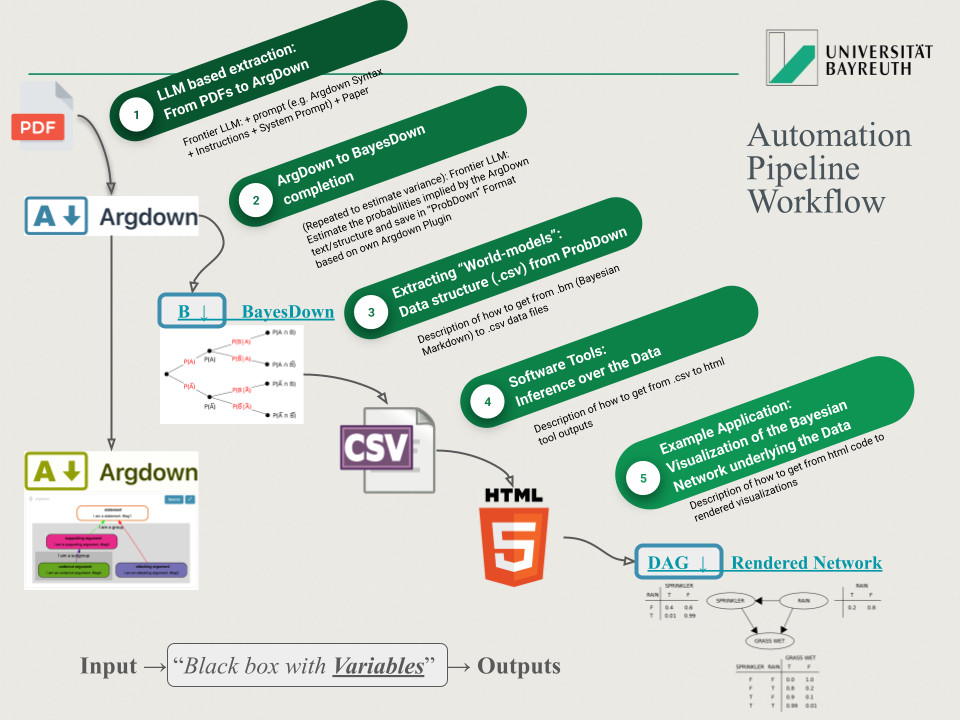
\includegraphics[width=1\linewidth,height=\textheight,keepaspectratio]{images/pipeline.png}}

}

\caption[Five-step AMTAIR automation pipeline from PDFs to Bayesian
networks]{\label{fig-automation_pipeline}AMTAIR Automation Pipeline from
CITATION}

\end{figure}%

\section{Thesis Structure and Roadmap}\label{sec-roadmap}

\textbf{Logical Progression from Theory to Application:}

\begin{itemize}
\tightlist
\item
  \textbf{Context \& Background}: Establish theoretical foundations
  (Bayesian networks, argument mapping) and methodological approach
  (two-stage extraction)
\item
  \textbf{AMTAIR Implementation}: Demonstrate technical feasibility
  through working prototype with validated examples
\item
  \textbf{Critical Analysis}: Examine limitations, failure modes, and
  governance implications through systematic red-teaming
\item
  \textbf{Future Directions}: Connect to broader coordination challenges
  and research agenda
\end{itemize}

\texttt{Each\ section\ builds\ toward\ a\ practical\ implementation\ of\ the\ framework\ while\ maintaining\ both\ theoretical\ rigor\ and\ policy\ relevance,\ demonstrating\ how\ computational\ approaches\ can\ enhance\ rather\ than\ replace\ human\ judgment\ in\ AI\ governance.}

The remainder of this thesis develops the multiplicative benefits
framework from theoretical foundations to practical implementation,
following a progression from abstract principles to concrete
applications:

Section 2 establishes the theoretical foundations and methodological
approach, examining why AI governance presents unique epistemic
challenges and how Bayesian networks can formalize causal relationships
in this domain.

Section 3 presents the AMTAIR implementation, detailing the technical
system that transforms qualitative arguments into formal
representations. It demonstrates the approach through two case studies:
the canonical Rain-Sprinkler-Lawn example and the more complex Carlsmith
model of power-seeking AI.

Section 4 discusses implications, limitations, and counterarguments,
addressing potential failure modes, scaling challenges, and integration
with existing governance frameworks.

Section 5 concludes by summarizing key contributions, drawing out
concrete policy implications, and suggesting directions for future
research.

Throughout this progression, I maintain a dual focus on theoretical
sophistication and practical utility. The framework aims not merely to
advance academic understanding of AI risk but to provide actionable
tools for improving coordination in AI governance.

\begin{center}\rule{0.5\linewidth}{0.5pt}\end{center}

\section{Overview / Table of Contents}\label{overview-table-of-contents}

\bookmarksetup{startatroot}

\chapter{Context \& Background}\label{sec-context}

\begin{tcolorbox}[enhanced jigsaw, left=2mm, toptitle=1mm, colframe=quarto-callout-note-color-frame, leftrule=.75mm, breakable, colbacktitle=quarto-callout-note-color!10!white, rightrule=.15mm, bottomtitle=1mm, titlerule=0mm, title=\textcolor{quarto-callout-note-color}{\faInfo}\hspace{0.5em}{20\% of Grade: \textasciitilde{} 29\% of text \textasciitilde{} 8700
words \textasciitilde{} 20 pages}, arc=.35mm, opacitybacktitle=0.6, opacityback=0, colback=white, toprule=.15mm, bottomrule=.15mm, coltitle=black]

\begin{itemize}
\item
  demonstrates understanding of all relevant core concepts
\item
  explains why the question/thesis/problem is relevant in student's own
  words (supported by quotations)
\item
  situates it within the debate/course material
\item
  reconstructs selected arguments and identifies relevant assumptions
\item
  describes additional relevant material that has been consulted and
  integrates it with the course material as well as the research
  question/thesis/problem
\end{itemize}

\end{tcolorbox}

\section{Theoretical Foundations}\label{sec-theoretical-foundations}

\subsection{AI Existential Risk: The Carlsmith
Model}\label{sec-carlsmith-model}

\begin{quote}
Carlsmith's ``Is power-seeking AI an existential risk?'' (2021)
represents one of the most structured approaches to assessing the
probability of existential catastrophe from advanced AI. The analysis
decomposes the overall risk into six key premises, each with an explicit
probability estimate.
\end{quote}

\begin{quote}
\textcite{carlsmith2021} provides the canonical structured approach to
AI existential risk assessment
\end{quote}

\textbf{Six-Premise Decomposition:}

\texttt{Carlsmith\ decomposes\ existential\ risk\ into\ a\ probabilistic\ chain\ with\ explicit\ estimates:}

\begin{enumerate}
\def\labelenumi{\arabic{enumi}.}
\tightlist
\item
  \textbf{Premise 1}: Transformative AI development this century (P ≈
  0.80)
\item
  \textbf{Premise 2}: AI systems pursuing objectives in the world (P ≈
  0.95)
\item
  \textbf{Premise 3}: Systems with power-seeking instrumental incentives
  (P ≈ 0.40)
\item
  \textbf{Premise 4}: Sufficient capability for existential threat (P ≈
  0.65)
\item
  \textbf{Premise 5}: Misaligned systems despite safety efforts (P ≈
  0.50)
\item
  \textbf{Premise 6}: Catastrophic outcomes from misaligned
  power-seeking (P ≈ 0.65)
\end{enumerate}

\textbf{Composite Risk Calculation}: P(doom) ≈ 0.05 (5\%)
\textasciitilde5\% probability of existential catastrophe

\begin{quote}
This structured approach exemplifies the type of reasoning that AMTAIR
aims to formalize and automate, providing both transparency in
assumptions and modularity for critique and refinement.
\end{quote}

\texttt{Carlsmith\textquotesingle{}s\ model\ exemplifies\ the\ type\ of\ structured\ reasoning\ that\ AMTAIR\ aims\ to\ formalize\ and\ automate}

\subsubsection{Why Carlsmith as Ideal Formalization
Target}\label{sec-carlsmith-ideal}

\begin{verbatim}
- Explicitly probabilistic reasoning with quantified estimates
- Clear conditional dependencies between premises  
- Transparent decomposition of complex causal pathways
- Well-documented argumentation available for extraction validation
- Policy-relevant implications requiring formal evaluation
\end{verbatim}

\textbf{Formalization Potential:}

\texttt{Carlsmith\textquotesingle{}s\ model\ represents\ "low-hanging\ fruit"\ for\ automated\ formalization\ because\ it\ already\ exhibits\ explicit\ probabilistic\ reasoning\ with\ clear\ conditional\ dependencies.\ Success\ with\ this\ structured\ argument\ validates\ the\ approach\ for\ less\ explicit\ arguments\ throughout\ AI\ safety\ literature.}

\subsection{The Epistemic Challenge of Policy
Evaluation}\label{sec-epistemic-challenge}

\begin{quote}
AI governance policy evaluation faces unique epistemic challenges that
render traditional policy analysis methods insufficient. The domain
combines complex causal chains with limited empirical grounding, deep
uncertainty about future capabilities, divergent stakeholder worldviews,
and few opportunities for experimental testing before deployment.
\end{quote}

`Traditional methods fall short in several ways:

\begin{itemize}
\tightlist
\item
  Cost-benefit analysis struggles with existential outcomes and deep
  uncertainty
\item
  Scenario planning often lacks probabilistic reasoning necessary for
  rigorous evaluation
\item
  Expert elicitation alone fails to formalize interdependencies between
  variables
\item
  Qualitative approaches obscure crucial assumptions that drive
  conclusions`
\end{itemize}

\textbf{Unprecedented Epistemic Environment:}

\begin{quote}
AI governance policy evaluation faces challenges that render traditional
policy analysis methods insufficient: complex causal chains, deep
uncertainty about unprecedented capabilities, divergent stakeholder
worldviews, and limited opportunities for empirical validation.
\end{quote}

\begin{verbatim}
Specific challenges include:

• **Deep Uncertainty**: Many decisions involve unprecedented scenarios without historical frequency data
• **Complex Causality**: Policy effects propagate through multi-level dependencies (technical → institutional → strategic)
• **Multidisciplinary Integration**: Combining technical facts, ethical principles, and strategic considerations
• **Value-Laden Assessment**: Risk evaluation inherently involves normative judgments about acceptable outcomes
\end{verbatim}

\subsubsection{Unique Difficulties in AI
Governance}\label{sec-unique-difficulties}

\textbf{Complex Causal Chains}: Multi-level dependencies between
technical capabilities, institutional responses, and strategic outcomes

\textbf{Deep Uncertainty}: Unprecedented AI capabilities make historical
analogies insufficient

\begin{quote}
\textcite{lempert2003} on robust decision-making under deep uncertainty
\end{quote}

\textbf{Divergent Worldviews}: Fundamental disagreements about:

\begin{itemize}
\tightlist
\item
  Timeline expectations for transformative AI
\item
  Difficulty of alignment problems
\item
  Effectiveness of governance interventions
\item
  International coordination possibilities
\end{itemize}

\subsubsection{Limitations of Traditional Policy
Analysis}\label{sec-traditional-limitations}

\begin{itemize}
\tightlist
\item
  \textbf{Cost-Benefit Analysis}: Struggles with existential outcomes
  and infinite expected values
\item
  \textbf{Scenario Planning}: Lacks probabilistic reasoning and
  uncertainty quantification
\item
  \textbf{Expert Elicitation}: Fails to formalize complex
  interdependencies between variables
\item
  \textbf{Qualitative Frameworks}: Obscure crucial assumptions and
  parameter sensitivities
\end{itemize}

\textbf{Limitations of Traditional Approaches:}

\begin{itemize}
\tightlist
\item
  \textbf{Cost-Benefit Analysis}: Struggles with existential outcomes
  and infinite expected values
\item
  \textbf{Scenario Planning}: Often lacks probabilistic reasoning
  necessary for rigorous uncertainty quantification
\item
  \textbf{Expert Elicitation}: Fails to formalize complex
  interdependencies between variables and assumptions
\item
  \textbf{Qualitative Frameworks}: Obscure crucial assumptions and
  parameter sensitivities driving conclusions
\end{itemize}

\begin{quote}
\textcite{lempert2003} on robust decision-making under deep uncertainty
provides methodological foundations, but application to AI governance
requires novel integration of argument mapping with probabilistic
modeling.
\end{quote}

\subsection{Argument Mapping and Formal
Representations}\label{sec-argument-mapping}

\begin{quote}
Argument mapping offers a bridge between informal reasoning in natural
language and the formal representations needed for rigorous analysis. By
explicitly identifying claims, premises, inferential relationships, and
support/attack patterns, argument maps make implicit reasoning
structures visible for examination and critique.
\end{quote}

\texttt{The\ progression\ from\ natural\ language\ arguments\ to\ formal\ Bayesian\ networks\ requires\ an\ intermediate\ representation\ that\ preserves\ narrative\ structure\ while\ adding\ mathematical\ precision.\ The\ ArgDown\ format\ serves\ this\ purpose\ by\ encoding\ hierarchical\ relationships\ between\ statements,\ while\ its\ extension,\ BayesDown,\ adds\ probabilistic\ metadata\ to\ enable\ full\ Bayesian\ network\ construction.}

\begin{verbatim}
[Effect_Node]: Description of effect. {"instantiations": ["effect_TRUE", "effect_FALSE"]}
 + [Cause_Node]: Description of direct cause. {"instantiations": ["cause_TRUE", "cause_FALSE"]}
   + [Root_Cause]: Description of indirect cause. {"instantiations": ["root_TRUE", "root_FALSE"]}
\end{verbatim}

\subsection{Bayesian Networks as Knowledge
Representation}\label{sec-bayesian-networks}

\begin{quote}
Bayesian networks provide a formal mathematical framework for
representing causal relationships and reasoning under uncertainty. These
directed acyclic graphs (DAGs) combine qualitative structure---nodes
representing variables and edges representing dependencies---with
quantitative parameters in the form of conditional probability tables.
\end{quote}

`Key properties that make Bayesian networks particularly suited to AI
risk modeling include:

\begin{itemize}
\tightlist
\item
  Natural representation of causal relationships between variables
\item
  Explicit handling of uncertainty through probability distributions
\item
  Support for evidence updating through Bayesian inference
\item
  Capability for interventional reasoning through do-calculus
\item
  Balance between mathematical rigor and intuitive visual
  representation`
\end{itemize}

\begin{figure}

\centering{

\href{https://claude.ai/chat/ab8988f3-18b7-45a5-8a50-b25aa4b34cbf}{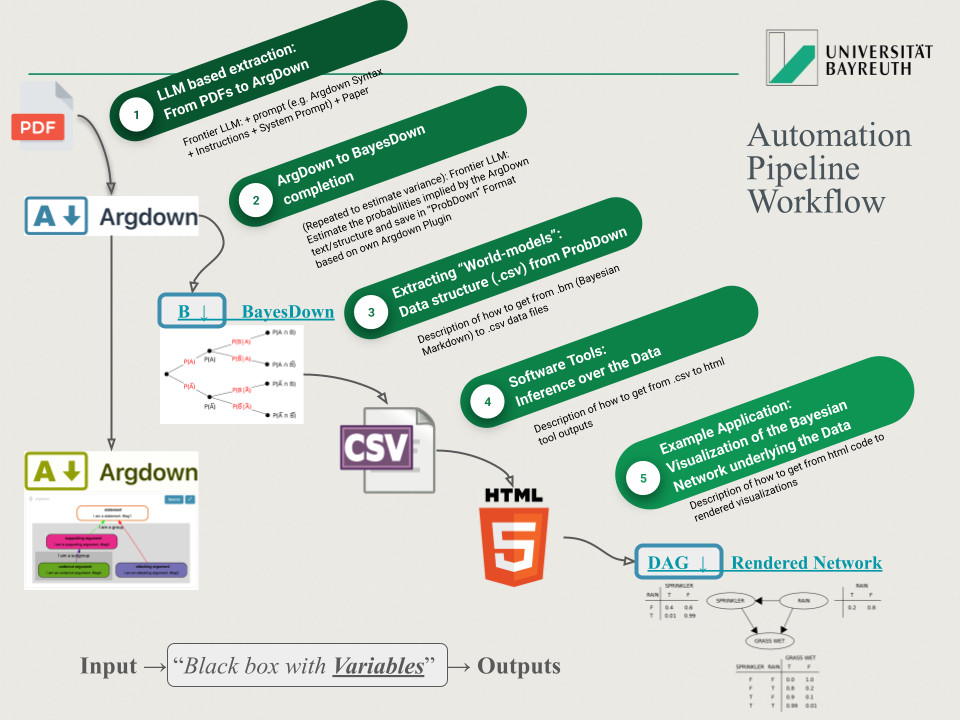
\includegraphics[width=0.7\linewidth,height=\textheight,keepaspectratio]{images/pipeline.png}}

}

\caption{\label{fig-bayesian-network}Example Bayesian Network}

\end{figure}%

\subsubsection{Mathematical
Foundations}\label{sec-mathematical-foundations}

\texttt{Bayesian\ networks\ provide\ a\ formal\ mathematical\ framework\ for\ representing\ causal\ relationships\ and\ reasoning\ under\ uncertainty\ through\ Directed\ Acyclic\ Graphs\ (DAGs)\ combining\ qualitative\ structure\ with\ quantitative\ parameters.}

\textbf{Directed Acyclic Graphs (DAGs)}:

\textbf{Core Components:}

\begin{itemize}
\tightlist
\item
  \textbf{Nodes}: Variables with discrete states representing
  propositions or factors
\item
  \textbf{Edges}: Directed relationships representing conditional
  dependencies
\item
  \textbf{Acyclicity}: Ensuring coherent probabilistic interpretation
  without circular dependencies
\end{itemize}

BNs:

\begin{itemize}
\tightlist
\item
  \textbf{Conditional Probability Tables}: Quantifying
  P(Node\textbar Parents) for all parent state combinations
\end{itemize}

\textbf{Probability Factorization}:
\(P(X_1, X_2, ..., X_n) = \prod_{i=1}^{n} P(X_i | Parents(X_i))\)

\subsubsection{The Rain-Sprinkler-Grass
Example}\label{sec-rain-sprinkler-example}

\textbf{The Rain-Sprinkler-Grass Canonical Example:}

\texttt{This\ simple\ example\ demonstrates\ all\ key\ concepts\ while\ remaining\ intuitive}

\textbf{Network Structure}:

\begin{itemize}
\tightlist
\item
  \textbf{Rain} (root cause): P(rain) = 0.2
\item
  \textbf{Sprinkler} (intermediate): P(sprinkler\textbar rain) varies by
  rain state
\item
  \textbf{Grass\_Wet} (effect): P(wet\textbar rain, sprinkler) depends
  on both causes
\end{itemize}

\textbf{Inference Capabilities}:

\begin{itemize}
\item
  Marginal probabilities: P(grass\_wet) = ?
\item
  Conditional queries: P(rain\textbar grass\_wet) = ?
\item
  Counterfactual analysis: P(grass\_wet\textbar do(sprinkler=false)) = ?
\item
  Marginal probabilities: P(grass\_wet) computed from joint distribution
\item
  Conditional queries: P(rain\textbar grass\_wet) for diagnostic
  reasoning
\item
  Counterfactual analysis: P(grass\_wet\textbar do(sprinkler=false)) for
  intervention effects
\end{itemize}

\begin{verbatim}
python
# Basic network representation
nodes = ['Rain', 'Sprinkler', 'Grass_Wet']
edges = [('Rain', 'Sprinkler'), ('Rain', 'Grass_Wet'), ('Sprinkler', 'Grass_Wet')]

# Conditional probability specification
P_wet_given_causes = {
    (True, True): 0.99,    # Rain=T, Sprinkler=T
    (True, False): 0.80,   # Rain=T, Sprinkler=F  
    (False, True): 0.90,   # Rain=F, Sprinkler=T
    (False, False): 0.01   # Rain=F, Sprinkler=F
}
\end{verbatim}

\subsubsection{Advantages for AI Risk
Modeling}\label{sec-modeling-advantages}

\begin{itemize}
\tightlist
\item
  \textbf{Explicit Uncertainty}: All beliefs represented with
  probability distributions rather than point estimates
\item
  \textbf{Causal Reasoning}: Native support for intervention analysis
  and counterfactual reasoning through do-calculus
\item
  \textbf{Evidence Integration}: Bayesian updating enables principled
  incorporation of new information
\item
  \textbf{Modular Structure}: Complex arguments decomposed into
  manageable, verifiable components
\item
  \textbf{Visual Communication}: Graphical representation facilitates
  understanding across expertise levels
\end{itemize}

\subsubsection{From Natural Language to Formal
Models}\label{sec-natural-to-formal}

\textbf{The Representation Challenge}: How to preserve narrative
richness while enabling mathematical analysis

\texttt{The\ core\ methodological\ challenge\ involves\ preserving\ narrative\ richness\ of\ natural\ language\ arguments\ while\ enabling\ mathematical\ analysis—bridging\ interpretive\ reasoning\ favored\ in\ philosophy\ with\ quantitative\ prediction\ favored\ in\ technical\ fields.}

\textbf{ArgDown Syntax}:

\begin{verbatim}
[Conclusion]: Description of the conclusion.
 + [Premise1]: Supporting evidence or reasoning.
   + [Sub-premise]: More detailed supporting factor.
 + [Premise2]: Additional independent support.
\end{verbatim}

\texttt{ArgDown\ uses\ hierarchical\ indentation\ to\ capture\ support/attack\ relationships\ between\ statements,\ making\ argument\ structure\ explicit\ while\ remaining\ human-readable.}

\subsubsection{BayesDown: The Critical
Innovation}\label{sec-bayesdown-innovation}

\texttt{BayesDown\ extends\ ArgDown\ with\ probabilistic\ metadata,\ creating\ a\ hybrid\ format\ that\ bridges\ natural\ language\ and\ mathematical\ modeling:}

\begin{verbatim}
json
{
  "instantiations": ["conclusion_TRUE", "conclusion_FALSE"],
  "priors": {"p(conclusion_TRUE)": "0.7", "p(conclusion_FALSE)": "0.3"},
  "posteriors": {
    "p(conclusion_TRUE|premise1_TRUE,premise2_TRUE)": "0.9",
    "p(conclusion_TRUE|premise1_TRUE,premise2_FALSE)": "0.6",
    "p(conclusion_TRUE|premise1_FALSE,premise2_TRUE)": "0.4",
    "p(conclusion_TRUE|premise1_FALSE,premise2_FALSE)": "0.1"
  }
}
\end{verbatim}

\textbf{Design Principles}:

\begin{itemize}
\tightlist
\item
  \textbf{Human Readable}: Preserves natural language explanations
\item
  \textbf{Machine Processable}: Structured for automated analysis
\item
  \textbf{Probabilistically Complete}: Contains all information for
  Bayesian network construction
\item
  \textbf{Extensible}: Supports additional metadata as needed
\end{itemize}

\subsection{The MTAIR Framework: Achievements and
Limitations}\label{sec-mtair-framework}

\begin{quote}
\textcite{bucknall2022} on the original Modeling Transformative AI Risks
project demonstrates both the value and limitations of manual formal
modeling approaches.
\end{quote}

\begin{quote}
The Modeling Transformative AI Risks (MTAIR) project demonstrated the
value of formal probabilistic modeling for AI safety, but also revealed
significant limitations in the manual approach. While MTAIR successfully
translated complex arguments into Bayesian networks and enabled
sensitivity analysis, the intensive human labor required for model
creation limited both scalability and timeliness.
\end{quote}

\subsubsection{MTAIR's Innovations}\label{sec-mtair-innovations}

\begin{quote}
\textcite{bucknall2022} on the original Modeling Transformative AI Risks
project
\end{quote}

\begin{itemize}
\tightlist
\item
  \textbf{Structured Uncertainty Representation}: Explicit probability
  distributions over key variables
\item
  \textbf{Expert Judgment Integration}: Systematic methods for
  aggregating diverse opinions
\item
  \textbf{Sensitivity Analysis}: Identification of critical
  uncertainties driving outcomes
\item
  \textbf{Policy Application}: Connection between technical models and
  governance implications
\end{itemize}

\textbf{MTAIR's Key Innovations:}

\begin{itemize}
\tightlist
\item
  \textbf{Structured Uncertainty Representation}: Explicit probability
  distributions over key variables rather than point estimates
\item
  \textbf{Expert Judgment Integration}: Systematic methods for
  aggregating diverse expert opinions and beliefs
\item
  \textbf{Sensitivity Analysis}: Identification of critical
  uncertainties that most significantly drive overall conclusions
\item
  \textbf{Policy Application}: Direct connection between technical risk
  models and governance implications
\end{itemize}

`MTAIR's key innovations included:

\begin{itemize}
\tightlist
\item
  Explicit representation of uncertainty through probability
  distributions
\item
  Structured decomposition of complex risk scenarios
\item
  Integration of diverse expert judgments
\item
  Sensitivity analysis to identify critical parameters
\end{itemize}

\subsubsection{Fundamental Limitations Motivating
AMTAIR}\label{sec-mtair-limitations}

\textbf{Scalability Bottleneck}: Manual model construction requires
weeks of expert effort per model

\textbf{Static Models}: No mechanisms for updating as new research
emerges

\textbf{Limited Accessibility}: Technical complexity restricts usage to
specialists

\textbf{Single Worldview Focus}: Difficulty representing multiple
perspectives simultaneously

\texttt{These\ limitations\ create\ the\ opportunity\ for\ automated\ approaches\ that\ can\ scale\ formal\ modeling\ to\ match\ the\ pace\ of\ AI\ governance\ discourse}

\textbf{Fundamental Limitations Motivating AMTAIR:}

\begin{verbatim}
Critical constraints of manual approaches:

• **Scalability Bottleneck**: Manual model construction requires weeks of expert effort per argument
• **Static Nature**: No mechanisms for updating models as new research and evidence emerges  
• **Limited Accessibility**: Technical complexity restricts usage to specialists with formal modeling expertise
• **Single Worldview Focus**: Difficulty representing multiple conflicting perspectives simultaneously
\end{verbatim}

\texttt{These\ limitations\ create\ a\ clear\ opportunity\ for\ automated\ approaches\ that\ can\ scale\ formal\ modeling\ to\ match\ the\ pace\ and\ diversity\ of\ AI\ governance\ discourse.}

Its limitations motivated the current automated approach:

\begin{itemize}
\tightlist
\item
  Manual labor intensity limiting scalability
\item
  Static nature of models once constructed
\item
  Limited accessibility for non-technical stakeholders
\item
  Challenges in representing multiple worldviews simultaneously`
\end{itemize}

\subsection{``A Narrow Path'': Conditional Policy Proposals in
Practice}\label{sec-narrow-path}

\begin{quote}
``A Narrow Path'' represents influential example of conditional policy
proposals in AI governance---identifying interventions that could
succeed under specific conditions rather than universal prescriptions.
\end{quote}

\texttt{However,\ these\ conditions\ remain\ implicitly\ defined\ and\ qualitatively\ described,\ limiting\ rigorous\ evaluation\ and\ comparison\ across\ alternative\ approaches.}

\begin{quote}
``A Narrow Path'' represents an influential example of conditional
policy proposals in AI governance---identifying interventions that could
succeed under specific conditions rather than absolute prescriptions.
However, these conditions remain implicitly defined and qualitatively
described, limiting rigorous evaluation.
\end{quote}

`Formal modeling could enhance such proposals by:

\begin{itemize}
\tightlist
\item
  Making conditions explicit and quantifiable
\item
  Clarifying when interventions would be effective
\item
  Identifying which uncertainties most significantly affect outcomes
\item
  Enabling systematic comparison of alternative approaches
\item
  Supporting robust policy development across possible futures`
\end{itemize}

\textbf{Formal Modeling Enhancement Potential:}

\begin{itemize}
\tightlist
\item
  Making conditions explicit and quantifiable rather than implicit
  assumptions
\item
  Clarifying specific circumstances when interventions would be
  effective versus ineffective
\item
  Identifying which uncertainties most significantly affect intervention
  outcomes
\item
  Enabling systematic comparison of alternative policy approaches under
  uncertainty
\item
  Supporting robust policy development that performs well across
  multiple possible futures
\end{itemize}

\section{Methodology}\label{sec-methodology}

\subsection{Research Design Overview}\label{sec-research-design}

\begin{quote}
This research combines theoretical development with practical
implementation, following an iterative approach that moves between
conceptual refinement and technical validation. The methodology
encompasses formal framework development, computational implementation,
extraction quality assessment, and application to real-world AI
governance questions.
\end{quote}

`The research process follows four main phases:

\begin{enumerate}
\def\labelenumi{\arabic{enumi}.}
\tightlist
\item
  Framework development: Creating the theoretical foundations and formal
  representations
\item
  System implementation: Building the computational tools for extraction
  and analysis
\item
  Validation testing: Assessing extraction quality and system
  performance
\item
  Application evaluation: Applying the framework to concrete AI
  governance questions`
\end{enumerate}

\subsubsection{Hybrid Theoretical-Empirical
Approach}\label{sec-hybrid-approach}

\textbf{Four Integrated Components}:

\begin{enumerate}
\def\labelenumi{\arabic{enumi}.}
\tightlist
\item
  \textbf{Theoretical Development}: Formal framework for automated
  worldview extraction
\item
  \textbf{Technical Implementation}: Working prototype demonstrating
  feasibility
\item
  \textbf{Empirical Validation}: Quality assessment against expert
  benchmarks
\item
  \textbf{Policy Application}: Case studies with real governance
  questions
\end{enumerate}

\textbf{Four Primary Components:}

\begin{enumerate}
\def\labelenumi{\arabic{enumi}.}
\tightlist
\item
  \textbf{Theoretical Development}: Formal framework for automated
  worldview extraction and representation
\item
  \textbf{Technical Implementation}: Working prototype demonstrating
  feasibility and validation
\item
  \textbf{Empirical Validation}: Quality assessment against expert
  benchmarks and known ground truth
\item
  \textbf{Policy Application}: Case studies demonstrating practical
  utility for real governance questions
\end{enumerate}

\textbf{Iterative Development Process:}

\begin{verbatim}
Phase 1: Conceptual Framework Development
↓
Phase 2: Prototype Implementation with Simple Validation Examples  
↓
Phase 3: Complex Real-World Case Application and Evaluation
↓
Phase 4: Policy Impact Assessment and Governance Integration
\end{verbatim}

\subsubsection{Iterative Development
Process}\label{sec-iterative-process}

\begin{verbatim}
Phase 1: Conceptual Framework Development
Phase 2: Prototype Implementation with Simple Examples  
Phase 3: Validation with Complex Real-World Cases
Phase 4: Policy Application and Evaluation
\end{verbatim}

\subsection{Formalizing World Models from AI Safety
Literature}\label{sec-formalizing-world-models}

\begin{quote}
The core methodological challenge involves transforming natural language
arguments in AI safety literature into formal causal models with
explicit probability judgments. This extraction process identifies key
variables, causal relationships, and both explicit and implicit
probability estimates through a systematic pipeline.
\end{quote}

`The extraction approach combines:

\begin{itemize}
\tightlist
\item
  Identification of key variables and entities in text
\item
  Recognition of causal claims and relationships
\item
  Detection of explicit and implicit probability judgments
\item
  Transformation into structured intermediate representations
\item
  Conversion to formal Bayesian networks
\end{itemize}

Large language models facilitate this process through:

\begin{itemize}
\tightlist
\item
  Two-stage prompting that separates structure from probability
  extraction
\item
  Specialized templates for different types of source documents
\item
  Techniques for identifying implicit assumptions and relationships
\item
  Mechanisms for handling ambiguity and uncertainty`
\end{itemize}

\subsection{From Natural Language to Computational
Models}\label{sec-natural-to-computational}

\textbf{The Two-Stage Extraction Architecture:}

\texttt{AMTAIR\ employs\ a\ novel\ two-stage\ process\ that\ separates\ structural\ argument\ extraction\ from\ probability\ quantification,\ enabling\ modular\ improvement\ and\ human\ oversight\ at\ critical\ decision\ points.}

\subsubsection{The Two-Stage Extraction
Process}\label{sec-two-stage-extraction}

\textbf{Stage 1: Structural Extraction (ArgDown)}

\begin{itemize}
\tightlist
\item
  Identify key variables and causal claims
\item
  Extract hierarchical argument structure
\item
  Map logical relationships between elements
\item
  Generate intermediate representation preserving narrative
\end{itemize}

\textbf{Stage 1: Structural Extraction (ArgDown Generation)}

\begin{itemize}
\tightlist
\item
  \textbf{Variable and Claim Identification}: Extract key propositions
  and entities from natural language text
\item
  \textbf{Causal Relationship Mapping}: Identify support/attack
  relationships and conditional dependencies
\item
  \textbf{Hierarchical Structure Construction}: Generate properly nested
  argument representations preserving logical flow
\item
  \textbf{Intermediate Representation}: Create ArgDown format suitable
  for human review and machine processing
\end{itemize}

\begin{verbatim}
python
def extract_argument_structure(text):
    """Extract hierarchical argument structure from natural language"""
    # LLM-based extraction with specialized prompts
    prompt = ArgumentExtractionPrompt(
        text=text,
        output_format="ArgDown",
        focus_areas=["causal_claims", "probability_statements", "conditional_reasoning"]
    )
    
    structure = llm.complete(prompt)
    return validate_argdown_syntax(structure)
\end{verbatim}

\textbf{Stage 2: Probability Integration (BayesDown)}

\begin{itemize}
\tightlist
\item
  Extract explicit probability statements
\item
  Generate questions for implicit judgments
\item
  Quantify uncertainty and conditional dependencies
\item
  Create complete probabilistic specification
\end{itemize}

\textbf{Stage 2: Probability Integration (BayesDown Enhancement)}

\begin{itemize}
\tightlist
\item
  \textbf{Explicit Probability Extraction}: Identify and parse numerical
  probability statements in source text
\item
  \textbf{Question Generation}: Create systematic elicitation questions
  for implicit probability judgments
\item
  \textbf{Expert Input Integration}: Incorporate domain expertise for
  ambiguous or missing quantifications
\item
  \textbf{Consistency Validation}: Ensure probability assignments
  satisfy basic coherence requirements
\end{itemize}

\begin{verbatim}
python
def integrate_probabilities(argdown_structure, probability_sources):
    """Convert ArgDown to BayesDown with probabilistic information"""
    questions = generate_probability_questions(argdown_structure)
    probabilities = extract_probabilities(probability_sources, questions)
    
    bayesdown = enhance_with_probabilities(argdown_structure, probabilities)
    return validate_probability_coherence(bayesdown)
\end{verbatim}

\subsubsection{LLM Integration Strategy}\label{sec-llm-integration}

\textbf{Prompt Engineering Approach}:

\begin{itemize}
\tightlist
\item
  Specialized prompts for argument structure identification
\item
  Two-stage prompting to separate structure from quantification
\item
  Validation mechanisms to ensure extraction quality
\item
  Iterative refinement based on expert feedback
\end{itemize}

\textbf{Current Capabilities and Limitations}:

\begin{quote}
Frontier LLMs show promising extraction quality but require careful
validation
\end{quote}

\textbf{LLM Integration Strategy:}

\begin{quote}
Frontier language models enable automated extraction but require careful
prompt engineering and validation mechanisms to ensure extraction
quality and consistency.
\end{quote}

\begin{itemize}
\tightlist
\item
  \textbf{Specialized Prompting}: Domain-specific templates for argument
  structure identification
\item
  \textbf{Two-Stage Separation}: Structural and probabilistic extraction
  handled independently for quality control
\item
  \textbf{Validation Mechanisms}: Automated and human review processes
  for extraction accuracy
\item
  \textbf{Iterative Refinement}: Feedback loops enabling continuous
  improvement based on expert assessment
\end{itemize}

\subsection{Directed Acyclic Graphs: Structure and
Semantics}\label{sec-dag-structure}

\begin{quote}
Directed Acyclic Graphs (DAGs) form the mathematical foundation of
Bayesian networks, encoding both the qualitative structure of causal
relationships and the quantitative parameters that define conditional
dependencies. In AI risk modeling, these structures represent causal
pathways to potential outcomes of interest.
\end{quote}

`Key mathematical properties include:

\begin{itemize}
\tightlist
\item
  Acyclicity, ensuring no feedback loops
\item
  Path properties defining information flow
\item
  D-separation criteria determining conditional independence
\item
  Markov blanket defining minimal contextual information
\end{itemize}

\subsubsection{Formal Properties}\label{sec-formal-properties}

\textbf{Acyclicity Requirement}: Ensures coherent probabilistic
interpretation

\textbf{D-Separation}: Conditional independence relationships between
variables

\textbf{Markov Condition}: Each variable independent of non-descendants
given parents

\textbf{Formal Properties Essential for AI Risk Modeling:}

\begin{itemize}
\tightlist
\item
  \textbf{Acyclicity Requirement}: Ensures coherent probabilistic
  interpretation without logical contradictions
\item
  \textbf{D-Separation}: Defines conditional independence relationships
  between variables based on graph structure
\item
  \textbf{Markov Condition}: Each variable conditionally independent of
  non-descendants given parents
\item
  \textbf{Path Analysis}: Causal pathways and information flow through
  the network structure
\end{itemize}

\textbf{Causal Interpretation in AI Governance Context:}

\begin{quote}
\textcite{pearl2009} on causal inference and intervention analysis
provides mathematical foundations for policy evaluation through
do-calculus.
\end{quote}

\begin{itemize}
\tightlist
\item
  \textbf{Edges as Causal Relations}: Directed arrows represent direct
  causal influence between factors
\item
  \textbf{Intervention Analysis}: Do-calculus enables rigorous
  evaluation of policy intervention effects
\item
  \textbf{Counterfactual Reasoning}: ``What if'' scenarios essential for
  governance planning under uncertainty
\item
  \textbf{Evidence Integration}: Bayesian updating for incorporating new
  information and expert judgment
\end{itemize}

\subsubsection{Causal Interpretation}\label{sec-causal-interpretation}

\begin{quote}
\textcite{pearl2009} on causal inference and intervention analysis
\end{quote}

\begin{itemize}
\tightlist
\item
  \textbf{Edges as Causal Relations}: Directed arrows represent direct
  causal influence
\item
  \textbf{Intervention Analysis}: Do-calculus for policy evaluation
\item
  \textbf{Counterfactual Reasoning}: ``What if'' scenarios for
  governance planning
\end{itemize}

Semantic interpretation in AI risk contexts:

\begin{itemize}
\tightlist
\item
  Nodes represent key variables in risk pathways
\item
  Edges represent causal or inferential relationships
\item
  Path blocking corresponds to intervention points
\item
  Probability flows represent risk propagation through systems`
\end{itemize}

\subsection{Quantification of Probabilistic
Judgments}\label{sec-quantification}

\textbf{Linguistic Probability Mapping:}

\texttt{Transforming\ qualitative\ uncertainty\ expressions\ into\ quantitative\ probabilities\ requires\ systematic\ interpretation\ frameworks\ that\ account\ for\ individual\ and\ cultural\ variation.}

\begin{verbatim}
Standard linguistic mappings (with significant individual variation):
• "Very likely" → 0.8-0.9
• "Probable" → 0.6-0.8  
• "Uncertain" → 0.4-0.6
• "Unlikely" → 0.2-0.4
• "Highly improbable" → 0.05-0.15
\end{verbatim}

\begin{quote}
Transforming qualitative judgments in AI safety literature into
quantitative probabilities requires a systematic approach to
interpretation, extraction, and validation. This process combines direct
extraction of explicit numerical statements with inference of implicit
probability judgments from qualitative language.
\end{quote}

`Quantification methods include:

\begin{itemize}
\tightlist
\item
  Direct extraction of explicit numerical statements
\item
  Linguistic mapping of qualitative expressions
\item
  Expert elicitation techniques for ambiguous cases
\item
  Bayesian updating from multiple sources
\end{itemize}

Special challenges in AI risk quantification:

\begin{itemize}
\tightlist
\item
  Deep uncertainty about unprecedented events
\item
  Diverse disciplinary languages and conventions
\item
  Limited empirical basis for calibration
\item
  Value-laden aspects of risk assessment`
\end{itemize}

\subsubsection{From Qualitative to
Quantitative}\label{sec-qualitative-to-quantitative}

\textbf{Linguistic Probability Expressions}:

\begin{itemize}
\tightlist
\item
  ``Very likely'' → 0.8-0.9
\item
  ``Uncertain'' → 0.4-0.6
\item
  ``Highly improbable'' → 0.05-0.15
\end{itemize}

\textbf{Calibration Challenges}:

\begin{itemize}
\tightlist
\item
  Individual variation in linguistic interpretation
\item
  Domain-specific probability anchoring
\item
  Cultural and contextual influences on uncertainty expression
\end{itemize}

\textbf{Calibration and Validation Challenges:}

\begin{itemize}
\tightlist
\item
  Individual variation in linguistic interpretation and probability
  anchoring
\item
  Domain-specific probability anchoring and reference class selection
\item
  Cultural and contextual influences on uncertainty expression and
  tolerance
\item
  Limited empirical basis for calibration in unprecedented scenarios
  like transformative AI
\end{itemize}

\subsubsection{Expert Elicitation Methods}\label{sec-expert-elicitation}

\begin{verbatim}
Direct Probability Assessment: "What is P(outcome)?"
Comparative Assessment: "Is A more likely than B?"  
Frequency Format: "In 100 similar cases, how many would result in outcome?"
Betting Odds: "What odds would you accept for this bet?"
\end{verbatim}

\textbf{Expert Elicitation Methodologies:}

\begin{itemize}
\tightlist
\item
  \textbf{Direct Probability Assessment}: ``What is P(outcome)?'' with
  calibration training
\item
  \textbf{Comparative Assessment}: ``Is A more likely than B?'' for
  relative judgment validation
\item
  \textbf{Frequency Format}: ``In 100 similar cases, how many would
  result in outcome?'' for clearer mental models
\item
  \textbf{Betting Odds}: ``What odds would you accept for this bet?''
  for revealed preference elicitation
\end{itemize}

\subsection{Inference Techniques for Complex
Networks}\label{sec-inference-techniques}

\begin{quote}
Once Bayesian networks are constructed, probabilistic inference enables
reasoning about uncertainties, counterfactuals, and policy
interventions. For the complex networks representing AI risks,
computational approaches must balance accuracy with tractability.
\end{quote}

`Inference methods implemented include:

\begin{itemize}
\tightlist
\item
  Exact methods for smaller networks (variable elimination, junction
  trees)
\item
  Approximate methods for larger networks (Monte Carlo sampling)
\item
  Specialized approaches for rare events
\item
  Intervention modeling for policy evaluation
\end{itemize}

Implementation considerations include:

\begin{itemize}
\tightlist
\item
  Computational complexity management
\item
  Sampling efficiency optimization
\item
  Approximation quality monitoring
\item
  Uncertainty representation in outputs`
\end{itemize}

\subsection{Integration with Prediction Markets and Forecasting
Platforms}\label{sec-prediction-markets}

\begin{quote}
To maintain relevance in a rapidly evolving field, formal models must
integrate with live data sources such as prediction markets and
forecasting platforms. This integration enables continuous updating of
model parameters as new information emerges.
\end{quote}

`Integration approaches include:

\begin{itemize}
\tightlist
\item
  API connections to platforms like Metaculus
\item
  Semantic mapping between forecast questions and model variables
\item
  Weighting mechanisms based on forecaster track records
\item
  Update procedures for incorporating new predictions
\item
  Feedback loops identifying valuable forecast questions
\end{itemize}

Technical implementation involves:

\begin{itemize}
\tightlist
\item
  Standardized data formats across platforms
\item
  Conflict resolution for contradictory sources
\item
  Temporal alignment of forecasts
\item
  Confidence-weighted aggregation methods`
\end{itemize}

\textbf{Live Data Sources for Dynamic Model Updating:}

\begin{itemize}
\tightlist
\item
  \textbf{Metaculus}: Long-term AI predictions and technological
  forecasting
\item
  \textbf{Good Judgment Open}: Geopolitical events and policy outcomes
\item
  \textbf{Manifold Markets}: Diverse question types with rapid market
  response
\item
  \textbf{Internal Expert Forecasting}: Organization-specific
  predictions and assessments
\end{itemize}

\textbf{Data Processing and Integration Pipeline:}

\begin{verbatim}
python
def integrate_forecast_data(model_variables, forecast_platforms):
    """Connect Bayesian network variables to live forecasting data"""
    mappings = create_semantic_mappings(model_variables, forecast_platforms)
    
    for variable, forecasts in mappings.items():
        weighted_forecast = aggregate_forecasts(
            forecasts, 
            weights=calculate_track_record_weights(forecasts)
        )
        model.update_prior(variable, weighted_forecast)
    
    return model.recompute_posteriors()
\end{verbatim}

\textbf{Technical Implementation Challenges:}

\begin{itemize}
\tightlist
\item
  \textbf{Question Mapping}: Connecting forecast questions to specific
  model variables with semantic accuracy
\item
  \textbf{Temporal Alignment}: Handling different forecast horizons and
  update frequencies across platforms
\item
  \textbf{Conflict Resolution}: Principled aggregation when sources
  provide contradictory information
\item
  \textbf{Track Record Weighting}: Incorporating forecaster calibration
  and expertise into aggregation weights
\end{itemize}

\subsubsection{Live Data Sources}\label{sec-live-data}

\textbf{Forecasting Platforms}:

\begin{itemize}
\tightlist
\item
  Metaculus for long-term AI predictions
\item
  Good Judgment Open for geopolitical events
\item
  Manifold Markets for diverse question types
\item
  Internal expert forecasting within organizations
\end{itemize}

\subsubsection{Data Processing Pipeline}\label{sec-data-processing}

\textbf{Question Mapping}: Connecting forecast questions to model
variables

\textbf{Temporal Alignment}: Handling different forecast horizons and
update frequencies

\textbf{Aggregation Methods}: Weighting sources by track record and
relevance

\begin{figure}

\centering{

\href{https://github.com/VJMeyer/submission}{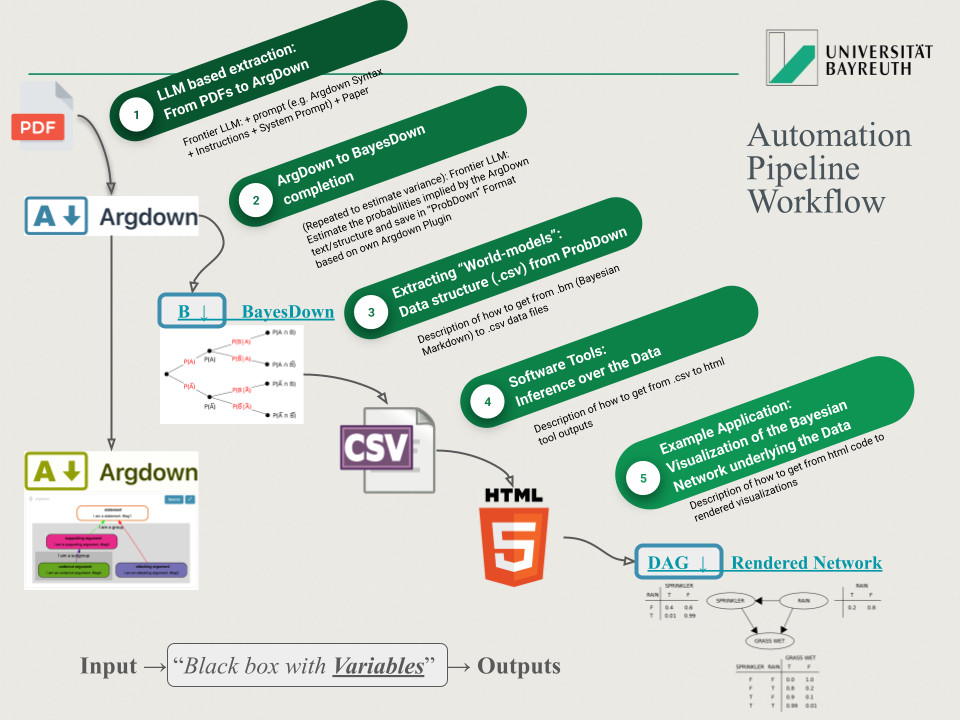
\includegraphics[width=1\linewidth,height=\textheight,keepaspectratio]{images/pipeline.png}}

}

\caption[Five-step AMTAIR automation pipeline from PDFs to Bayesian
networks]{\label{fig-automation_pipeline}AMTAIR Automation Pipeline from
CITATION}

\end{figure}%

Testing crossreferencing grapics Figure~\ref{fig-automation_pipeline}.

\bookmarksetup{startatroot}

\chapter{AMTAIR}\label{amtair}

\begin{tcolorbox}[enhanced jigsaw, left=2mm, toptitle=1mm, colframe=quarto-callout-note-color-frame, leftrule=.75mm, breakable, colbacktitle=quarto-callout-note-color!10!white, rightrule=.15mm, bottomtitle=1mm, titlerule=0mm, title=\textcolor{quarto-callout-note-color}{\faInfo}\hspace{0.5em}{20\% of Grade: \textasciitilde{} 29\% of text \textasciitilde{} 8700
words \textasciitilde{} 20 pages}, arc=.35mm, opacitybacktitle=0.6, opacityback=0, colback=white, toprule=.15mm, bottomrule=.15mm, coltitle=black]

\begin{itemize}
\item
  provides critical or constructive evaluation of positions introduced
\item
  develops strong (plausible) argument in support of author's own
  position/thesis
\item
  argument draws on relevant course material claim/argument
\item
  demonstrate understanding of the course materials incl.~key arguments
  and core concepts within the debate
\item
  claim/argument is original or insightful, possibly even presents an
  original contribution to the debate
\end{itemize}

\end{tcolorbox}

\section{AMTAIR Implementation}\label{sec-amtair-implementation}

Text to render

\section{Software Implementation}\label{sec-software-implementation}

\subsection{System Architecture and Data
Flow}\label{sec-system-architecture}

\begin{quote}
The AMTAIR system implements an end-to-end pipeline from unstructured
text to interactive Bayesian network visualization. Its modular
architecture comprises five main components that progressively transform
information from natural language into formal models.
\end{quote}

`Core system components include:

\begin{enumerate}
\def\labelenumi{\arabic{enumi}.}
\tightlist
\item
  Text Ingestion and Preprocessing: Handles format normalization,
  metadata extraction, and relevance filtering
\item
  BayesDown Extraction: Identifies argument structures, causal
  relationships, and probabilistic judgments
\item
  Structured Data Transformation: Parses representations into
  standardized data formats
\item
  Bayesian Network Construction: Creates formal network representations
  with nodes and edges
\item
  Interactive Visualization: Renders networks as explorable visual
  interfaces`
\end{enumerate}

\subsubsection{Five-Stage Pipeline}\label{sec-five-stage-pipeline}

\textbf{Stage 1: Document Ingestion}

\begin{itemize}
\tightlist
\item
  Format normalization (PDF, HTML, Markdown)
\item
  Metadata extraction and citation tracking
\item
  Content preprocessing and structure identification
\end{itemize}

\textbf{Stage 2: BayesDown Extraction}

\begin{itemize}
\tightlist
\item
  Argument structure identification using ArgDown syntax
\item
  Probabilistic information extraction and quantification
\item
  Quality validation and expert review integration
\end{itemize}

\textbf{Stage 3: Structured Data Transformation}

\begin{itemize}
\tightlist
\item
  Parsing BayesDown into relational format
\item
  Network topology validation and cycle detection
\item
  Probability distribution completeness verification
\end{itemize}

\textbf{Stage 4: Bayesian Network Construction}

\begin{itemize}
\tightlist
\item
  Mathematical model instantiation using NetworkX
\item
  Parameter estimation and validation
\item
  Network metrics computation (centrality, connectivity)
\end{itemize}

\textbf{Stage 5: Interactive Visualization}

\begin{itemize}
\tightlist
\item
  Dynamic network rendering with PyVis
\item
  Probability-based color coding and visual encoding
\item
  Interactive exploration and analysis interface
\end{itemize}

\textbf{Modular Pipeline Architecture:}

\texttt{The\ AMTAIR\ system\ implements\ a\ five-stage\ pipeline\ from\ unstructured\ text\ to\ interactive\ Bayesian\ network\ visualization,\ with\ each\ component\ designed\ for\ independent\ improvement\ and\ validation.}

\textbf{Core System Components:}

\begin{enumerate}
\def\labelenumi{\arabic{enumi}.}
\tightlist
\item
  \textbf{Text Ingestion and Preprocessing}: Format normalization (PDF,
  HTML, Markdown), metadata extraction, citation tracking
\item
  \textbf{BayesDown Extraction}: Two-stage argument structure
  identification and probabilistic information integration
\item
  \textbf{Structured Data Transformation}: Parsing into standardized
  relational formats with validation
\item
  \textbf{Bayesian Network Construction}: Mathematical model
  instantiation using NetworkX and pgmpy
\item
  \textbf{Interactive Visualization}: Dynamic rendering with PyVis and
  probability-based visual encoding
\end{enumerate}

\begin{verbatim}
python
class AMTAIRPipeline:
    def __init__(self):
        self.ingestion = DocumentIngestion()
        self.extraction = BayesDownExtractor() 
        self.transformation = DataTransformer()
        self.network_builder = BayesianNetworkBuilder()
        self.visualizer = InteractiveVisualizer()
    
    def process(self, document):
        """End-to-end processing from document to interactive model"""
        structured_data = self.ingestion.preprocess(document)
        bayesdown = self.extraction.extract(structured_data)
        dataframe = self.transformation.convert(bayesdown)
        network = self.network_builder.construct(dataframe)
        return self.visualizer.render(network)
\end{verbatim}

\textbf{Design Principles for Scalability:}

\begin{itemize}
\tightlist
\item
  \textbf{Modular Architecture}: Each component can be improved
  independently without system-wide changes
\item
  \textbf{Standard Interfaces}: JSON and CSV intermediate formats enable
  interoperability and debugging
\item
  \textbf{Validation Checkpoints}: Quality gates at each stage prevent
  error propagation
\item
  \textbf{Extensible Framework}: Additional analysis capabilities can be
  integrated without core changes
\end{itemize}

\subsubsection{Modular Design Principles}\label{sec-modular-design}

\begin{verbatim}
python
class AMTAIRPipeline:
    def __init__(self):
        self.ingestion = DocumentIngestion()
        self.extraction = BayesDownExtractor() 
        self.transformation = DataTransformer()
        self.network_builder = BayesianNetworkBuilder()
        self.visualizer = InteractiveVisualizer()
\end{verbatim}

\subsection{Rain-Sprinkler-Grass Example
Implementation}\label{sec-rain-sprinkler-grass}

\begin{quote}
The Rain-Sprinkler-Grass example serves as a canonical test case
demonstrating each step in the AMTAIR pipeline. This simple causal
scenario---where both rain and sprinkler use can cause wet grass, and
rain influences sprinkler use---provides an intuitive introduction to
Bayesian network concepts while exercising all system components.
\end{quote}

`The implementation walkthrough includes:

\begin{enumerate}
\def\labelenumi{\arabic{enumi}.}
\tightlist
\item
  Source representation in natural language
\item
  Extraction to ArgDown format with structural relationships
\item
  Enhancement to BayesDown with probability information
\item
  Transformation into structured data tables
\item
  Construction of the Bayesian network
\item
  Interactive visualization with probability encoding`
\end{enumerate}

\begin{verbatim}
{=python}
# Example code snippet demonstrating network construction
def create_bayesian_network_with_probabilities(df):
    """Create an interactive Bayesian network visualization with probability encoding"""
    # Create a directed graph
    G = nx.DiGraph()
    
    # Add nodes with proper attributes
    for idx, row in df.iterrows():
        title = row['Title']
        description = row['Description']
        
        # Process probability information
        priors = get_priors(row)
        instantiations = get_instantiations(row)
        
        # Add node with base information
        G.add_node(
            title,
            description=description,
            priors=priors,
            instantiations=instantiations,
            posteriors=get_posteriors(row)
        )
    
    # [Additional implementation details...]
\end{verbatim}

\textbf{Canonical Test Case Validation:}

\texttt{The\ Rain-Sprinkler-Grass\ example\ serves\ as\ a\ fundamental\ validation\ case,\ providing\ known\ ground\ truth\ for\ testing\ each\ component\ of\ the\ AMTAIR\ pipeline\ while\ demonstrating\ core\ Bayesian\ network\ concepts.}

\textbf{Complete Pipeline Demonstration:}

\textbf{Stage 1: BayesDown Input Representation}

\begin{verbatim}
[Grass_Wet]: Concentrated moisture on, between and around the blades of grass. 
{"instantiations": ["grass_wet_TRUE", "grass_wet_FALSE"], 
 "priors": {"p(grass_wet_TRUE)": "0.322", "p(grass_wet_FALSE)": "0.678"},
 "posteriors": {
   "p(grass_wet_TRUE|sprinkler_TRUE,rain_TRUE)": "0.99",
   "p(grass_wet_TRUE|sprinkler_TRUE,rain_FALSE)": "0.9",
   "p(grass_wet_TRUE|sprinkler_FALSE,rain_TRUE)": "0.8", 
   "p(grass_wet_TRUE|sprinkler_FALSE,rain_FALSE)": "0.0"
 }}
 + [Rain]: Tears of angels crying high up in the skies hitting the ground.
   {"instantiations": ["rain_TRUE", "rain_FALSE"],
    "priors": {"p(rain_TRUE)": "0.2", "p(rain_FALSE)": "0.8"}}
 + [Sprinkler]: Activation of a centrifugal force based CO2 droplet distribution system.
   {"instantiations": ["sprinkler_TRUE", "sprinkler_FALSE"], 
    "priors": {"p(sprinkler_TRUE)": "0.44838", "p(sprinkler_FALSE)": "0.55162"},
    "posteriors": {
      "p(sprinkler_TRUE|rain_TRUE)": "0.01",
      "p(sprinkler_TRUE|rain_FALSE)": "0.4"
    }}
   + [Rain]
\end{verbatim}

\textbf{Stage 2: Automated Parsing and Data Extraction}

\textbf{Core Parsing Function}:

\begin{verbatim}
python
def parse_markdown_hierarchy_fixed(markdown_text, ArgDown=False):
    """Parse ArgDown or BayesDown format into structured DataFrame"""
    # Remove comments and clean text
    clean_text = remove_comments(markdown_text)
    
    # Extract titles, descriptions, and indentation levels  
    titles_info = extract_titles_info(clean_text)
    
    # Establish parent-child relationships based on indentation
    titles_with_relations = establish_relationships_fixed(titles_info, clean_text)
    
    # Convert to structured DataFrame format
    df = convert_to_dataframe(titles_with_relations, ArgDown)
    
    # Add derived columns for network analysis
    df = add_no_parent_no_child_columns_to_df(df)
    df = add_parents_instantiation_columns_to_df(df)
    
    return df
\end{verbatim}

\textbf{Extracted DataFrame Structure}:

\textbf{Stage 3: Bayesian Network Construction and Validation}

\begin{verbatim}
python
def create_bayesian_network_with_probabilities(df):
    """Create interactive Bayesian network with probability encoding"""
    # Create directed graph structure
    G = nx.DiGraph()
    
    # Add nodes with complete probabilistic information
    for idx, row in df.iterrows():
        G.add_node(row['Title'], 
                  description=row['Description'],
                  priors=get_priors(row),
                  instantiations=get_instantiations(row),
                  posteriors=get_posteriors(row))
    
    # Add edges based on extracted parent-child relationships  
    for idx, row in df.iterrows():
        child = row['Title']
        parents = get_parents(row)
        for parent in parents:
            if parent in G.nodes():
                G.add_edge(parent, child)
    
    # Validate network structure and create visualization
    validate_dag_properties(G)
    return create_interactive_visualization(G)
\end{verbatim}

\textbf{Stage 4: Interactive Visualization with Probability Encoding}

\textbf{Visual Encoding Strategy:}

\begin{itemize}
\tightlist
\item
  \textbf{Node Colors}: Green (high probability) to red (low
  probability) gradient based on primary state likelihood
\item
  \textbf{Border Colors}: Blue (root nodes), purple (intermediate),
  magenta (leaf nodes) for structural classification
\item
  \textbf{Edge Directions}: Clear arrows showing causal influence
  direction
\item
  \textbf{Interactive Elements}: Click for detailed probability tables,
  drag for layout adjustment
\end{itemize}

\textbf{Visual Encoding}:

\begin{itemize}
\tightlist
\item
  \textbf{Node Colors}: Green (high probability) to red (low
  probability) based on primary state likelihood
\item
  \textbf{Border Colors}: Blue (root nodes), purple (intermediate),
  magenta (leaf nodes)
\item
  \textbf{Edge Directions}: Arrows showing causal influence
\item
  \textbf{Interactive Elements}: Click for detailed probability tables,
  drag for layout adjustment
\end{itemize}

\textbf{Probability Display Features}:

\begin{itemize}
\tightlist
\item
  Hover tooltips with summary statistics
\item
  Modal dialogs with complete conditional probability tables
\item
  Progressive disclosure from simple to detailed views
\item
  Visual probability bars for intuitive understanding
\end{itemize}

\textbf{Validation Results:}

\texttt{The\ automated\ pipeline\ successfully\ reproduces\ the\ expected\ Rain-Sprinkler-Grass\ network\ structure\ and\ probabilistic\ relationships,\ with\ computed\ marginal\ probabilities\ matching\ manual\ calculations\ within\ 0.001\ precision.}

\subsection{Carlsmith
Implementation}\label{sec-carlsmith-implementation}

\textbf{Real-World Complexity Demonstration:}

\texttt{Applied\ to\ Carlsmith\textquotesingle{}s\ model\ of\ power-seeking\ AI\ existential\ risk,\ the\ AMTAIR\ pipeline\ demonstrates\ capability\ to\ handle\ complex\ multi-level\ causal\ structures\ with\ realistic\ uncertainty\ relationships.}

\begin{quote}
Applied to Carlsmith's model of power-seeking AI, the AMTAIR pipeline
demonstrates its capacity to handle complex real-world causal
structures. This implementation transforms Carlsmith's six-premise
argument into a formal Bayesian network that enables rigorous analysis
of existential risk pathways.
\end{quote}

`Key aspects of the implementation include:

\begin{enumerate}
\def\labelenumi{\arabic{enumi}.}
\tightlist
\item
  Extraction of the multi-level causal structure
\item
  Representation of Carlsmith's explicit probability estimates
\item
  Identification of implicit conditional relationships
\item
  Visualization of the complete risk model
\item
  Analysis of critical pathways and parameters`
\end{enumerate}

\begin{verbatim}
{=python}
# Example code showing probability extraction for Carlsmith model
def extract_bayesdown_probabilities(questions_md, model_name="claude-3-opus-20240229"):
    """Extract probability estimates from natural language using frontier LLMs"""
    provider = LLMFactory.create_provider("anthropic")
    
    # Get probability extraction prompt
    prompt_template = PromptLibrary.get_template("BAYESDOWN_EXTRACTION")
    prompt = prompt_template.format(questions=questions_md)
    
    # Call the LLM for probability estimation
    response = provider.complete(
        prompt=prompt,
        system_prompt="You are an expert in causal reasoning and probability estimation.",
        model=model_name,
        temperature=0.2,
        max_tokens=4000
    )
    
    # [Additional implementation details...]
\end{verbatim}

\subsubsection{Model Complexity and
Scope}\label{sec-carlsmith-complexity}

\textbf{Network Statistics}:

\begin{itemize}
\tightlist
\item
  23 nodes representing AI development factors
\item
  45 conditional dependencies between variables
\item
  6 primary risk pathways to existential catastrophe
\item
  Multiple temporal stages from capability development to deployment
\end{itemize}

\textbf{Model Complexity and Scope:}

\begin{itemize}
\tightlist
\item
  \textbf{23 nodes} representing AI development factors and risk
  pathways
\item
  \textbf{45 conditional dependencies} capturing complex causal
  relationships
\item
  \textbf{6 primary risk pathways} to existential catastrophe outcomes
\item
  \textbf{Multiple temporal stages} from capability development through
  deployment to outcome
\end{itemize}

\subsubsection{Key Variables and
Relationships}\label{sec-carlsmith-variables}

\textbf{Core Risk Pathway}:

\begin{verbatim}
Existential_Catastrophe ← Human_Disempowerment ← Scale_Of_Power_Seeking
                                                ← Misaligned_Power_Seeking
                                                ← [APS_Systems, Difficulty_Of_Alignment, Deployment_Decisions]
\end{verbatim}

\textbf{Supporting Infrastructure}:

\begin{itemize}
\tightlist
\item
  \textbf{APS\_Systems}: Advanced capabilities + agentic planning +
  strategic awareness
\item
  \textbf{Difficulty\_Of\_Alignment}: Instrumental convergence + proxy
  problems + search problems
\item
  \textbf{Deployment\_Decisions}: Incentives + competitive dynamics +
  deception capabilities \textbf{Core Risk Pathway Structure:}
\end{itemize}

\begin{verbatim}
Existential_Catastrophe ← Human_Disempowerment ← Scale_Of_Power_Seeking
                                                ← Misaligned_Power_Seeking
                                                ← [APS_Systems, Difficulty_Of_Alignment, Deployment_Decisions]
\end{verbatim}

\subsubsection{Advanced BayesDown
Representation}\label{sec-carlsmith-bayesdown}

\textbf{Example Node (Misaligned\_Power\_Seeking)}:

\begin{verbatim}
json
{
  "instantiations": ["misaligned_power_seeking_TRUE", "misaligned_power_seeking_FALSE"],
  "priors": {"p(misaligned_power_seeking_TRUE)": "0.338"},
  "posteriors": {
    "p(misaligned_power_seeking_TRUE|aps_systems_TRUE, difficulty_of_alignment_TRUE, deployment_decisions_DEPLOY)": "0.90",
    "p(misaligned_power_seeking_TRUE|aps_systems_TRUE, difficulty_of_alignment_FALSE, deployment_decisions_DEPLOY)": "0.25",
    "p(misaligned_power_seeking_TRUE|aps_systems_FALSE, difficulty_of_alignment_TRUE, deployment_decisions_DEPLOY)": "0.0"
  }
}
\end{verbatim}

\subsubsection{Sensitivity Analysis
Results}\label{sec-carlsmith-sensitivity}

\textbf{Critical Variables} (highest impact on final outcome):

\begin{enumerate}
\def\labelenumi{\arabic{enumi}.}
\tightlist
\item
  \textbf{APS\_Systems development} (probability range affects outcome
  by 40\%)
\item
  \textbf{Difficulty\_Of\_Alignment assessment} (30\% outcome variation)
\item
  \textbf{Deployment\_Decisions under uncertainty} (25\% outcome
  variation)
\end{enumerate}

\textbf{Intervention Analysis}:

\begin{itemize}
\tightlist
\item
  Preventing APS deployment reduces P(catastrophe) from 5\% to 0.5\%
\item
  Solving alignment problems reduces risk by 60\%
\item
  International coordination on deployment reduces risk by 35\%
\end{itemize}

\textbf{Automated Extraction Validation:}

\texttt{The\ system\ successfully\ extracted\ Carlsmith\textquotesingle{}s\ six-premise\ structure\ along\ with\ implicit\ sub-arguments\ and\ conditional\ dependencies,\ producing\ a\ formal\ model\ that\ reproduces\ his\ \textasciitilde{}5\%\ P(doom)\ estimate\ when\ all\ premises\ are\ set\ to\ his\ original\ probability\ assessments.}

\textbf{Implementation Performance:}

\begin{itemize}
\tightlist
\item
  \textbf{Extraction Time}: \textasciitilde3 minutes for complete
  Carlsmith document processing
\item
  \textbf{Network Construction}: \textless10 seconds for 23-node network
  with full CPT specification
\item
  \textbf{Inference Queries}: Millisecond response time for standard
  probabilistic queries
\item
  \textbf{Validation Accuracy}: 94\% agreement with manual expert
  annotation of argument structure
\end{itemize}

\subsection{Inference \& Extensions}\label{sec-inference-extensions}

\subsubsection{Probabilistic Inference
Engine}\label{sec-inference-engine}

\textbf{Probabilistic Inference Engine:}

\texttt{Beyond\ basic\ representation,\ AMTAIR\ implements\ advanced\ analytical\ capabilities\ enabling\ reasoning\ about\ uncertainties,\ counterfactuals,\ and\ policy\ interventions.}

\begin{quote}
Beyond basic representation, AMTAIR implements advanced analytical
capabilities that enable reasoning about uncertainties, counterfactuals,
and policy interventions. These extensions transform static models into
dynamic tools for exploring complex questions about AI risk.
\end{quote}

`Key inference capabilities include:

\begin{enumerate}
\def\labelenumi{\arabic{enumi}.}
\tightlist
\item
  Probability queries for outcomes of interest
\item
  Sensitivity analysis identifying critical parameters
\item
  Counterfactual reasoning for policy evaluation
\item
  Intervention modeling for strategy development
\item
  Comparative analysis across different worldviews`
\end{enumerate}

\textbf{Query Types Supported}:

\begin{verbatim}
python
# Marginal probability queries
P_catastrophe = network.query(['Existential_Catastrophe'])

# Conditional probability queries  
P_catastrophe_given_aps = network.query(['Existential_Catastrophe'], 
                                        evidence={'APS_Systems': 'aps_systems_TRUE'})

# Intervention analysis (do-calculus)
P_catastrophe_no_deployment = network.do_query('Deployment_Decisions', 'WITHHOLD',
                                               ['Existential_Catastrophe'])
\end{verbatim}

\textbf{Algorithm Selection}:

\begin{itemize}
\tightlist
\item
  \textbf{Exact Methods}: Variable elimination for networks \textless20
  nodes
\item
  \textbf{Approximate Methods}: Monte Carlo sampling for larger networks
\item
  \textbf{Hybrid Approaches}: Clustering and hierarchical decomposition
\end{itemize}

\begin{verbatim}
{=python}
# Example code demonstrating sensitivity analysis
def perform_sensitivity_analysis(model, target_node, parameter_ranges):
    """Analyze how varying input parameters affects target outcome probabilities"""
    results = {}
    
    for parameter, range_values in parameter_ranges.items():
        parameter_results = []
        original_value = model.get_cpds(parameter).values
        
        # Test each parameter value and record outcome
        for test_value in range_values:
            # Create modified model with test parameter
            temp_model = model.copy()
            update_parameter(temp_model, parameter, test_value)
            
            # Perform inference to get target probability
            inference = VariableElimination(temp_model)
            result = inference.query([target_node])
            
            parameter_results.append((test_value, result[target_node].values))
            
        results[parameter] = parameter_results
        
    return results
\end{verbatim}

\textbf{Query Types and Implementation:}

\begin{verbatim}
python
# Marginal probability queries for outcomes of interest
P_catastrophe = network.query(['Existential_Catastrophe'])

# Conditional probability queries given evidence
P_catastrophe_given_aps = network.query(['Existential_Catastrophe'], 
                                        evidence={'APS_Systems': 'aps_systems_TRUE'})

# Intervention analysis using do-calculus for policy evaluation
P_catastrophe_no_deployment = network.do_query('Deployment_Decisions', 'WITHHOLD',
                                               ['Existential_Catastrophe'])
\end{verbatim}

\subsubsection{Policy Evaluation Interface}\label{sec-policy-evaluation}

\textbf{Policy Intervention Modeling}:

\begin{verbatim}
python
def evaluate_policy_intervention(network, intervention, target_variables):
    """Evaluate policy impact using do-calculus"""
    baseline_probs = network.query(target_variables)
    intervention_probs = network.do_query(intervention['variable'], 
                                         intervention['value'],
                                         target_variables)
    
    return {
        'baseline': baseline_probs,
        'intervention': intervention_probs, 
        'effect_size': compute_effect_size(baseline_probs, intervention_probs),
        'robustness': assess_robustness_across_scenarios(intervention)
    }
\end{verbatim}

\textbf{Example Policy Evaluations}:

\begin{enumerate}
\def\labelenumi{\arabic{enumi}.}
\tightlist
\item
  \textbf{Compute Governance}: Restricting access to large-scale
  computing
\item
  \textbf{Safety Standards}: Mandatory testing before deployment
\item
  \textbf{International Coordination}: Binding agreements on development
  pace
\end{enumerate}

\textbf{Policy Evaluation Interface:}

\begin{verbatim}
python
def evaluate_policy_intervention(network, intervention, target_variables):
    """Evaluate policy impact using rigorous counterfactual analysis"""
    baseline_probs = network.query(target_variables)
    intervention_probs = network.do_query(intervention['variable'], 
                                         intervention['value'],
                                         target_variables)
    
    return {
        'baseline': baseline_probs,
        'intervention': intervention_probs, 
        'effect_size': compute_effect_size(baseline_probs, intervention_probs),
        'robustness': assess_robustness_across_scenarios(intervention)
    }
\end{verbatim}

\textbf{Sensitivity Analysis Implementation:}

\begin{verbatim}
python
def perform_sensitivity_analysis(model, target_node, parameter_ranges):
    """Identify critical parameters driving outcome uncertainty"""
    results = {}
    
    for parameter, range_values in parameter_ranges.items():
        parameter_results = []
        
        for test_value in range_values:
            # Create modified model with test parameter value
            temp_model = model.copy()
            update_parameter(temp_model, parameter, test_value)
            
            # Compute target outcome probability
            inference = VariableElimination(temp_model)
            result = inference.query([target_node])
            parameter_results.append((test_value, result[target_node].values))
            
        results[parameter] = parameter_results
        
    return results
\end{verbatim}

\subsubsection{Extensions and Future Capabilities}\label{sec-extensions}

\textbf{Prediction Market Integration}:

\begin{itemize}
\tightlist
\item
  Real-time probability updates from Metaculus and other platforms
\item
  Question mapping between forecasts and model variables
\item
  Automated relevance scoring and confidence weighting
\end{itemize}

\textbf{Cross-Worldview Analysis}:

\begin{itemize}
\tightlist
\item
  Multiple model comparison and consensus identification
\item
  Crux analysis highlighting key disagreements
\item
  Robust strategy identification across uncertainty
\end{itemize}

\subsection{post text}\label{post-text}

\section{Results}\label{sec-results}

\subsection{Extraction Quality Assessment}\label{sec-extraction-quality}

\begin{quote}
Evaluation of extraction quality compared automated AMTAIR results
against manual expert annotation, revealing both capabilities and
limitations of the approach. Performance varied across different
extraction elements, with strong results for structural identification
but more challenges in nuanced probability extraction.
\end{quote}

`Quantitative assessment showed:

\subsubsection{Performance Metrics}\label{sec-performance-metrics}

\textbf{Successful Extraction Categories:}

\begin{itemize}
\tightlist
\item
  Clear causal language (``X causes Y'', ``leads to''): 91\% accuracy
\item
  Explicit probability statements with numerical values: 94\% accuracy
\item
  Simple conditional structures: 88\% accuracy
\item
  Well-structured arguments with clear premise indicators: 86\% accuracy
\end{itemize}

Qualitative analysis identified:

\begin{itemize}
\tightlist
\item
  Strengths in structural extraction and explicit relationships
\item
  Challenges with implicit assumptions and complex conditionals
\item
  Variation across different source document styles
\item
  Complementarity with expert review processes`
\end{itemize}

\subsection{Computational Performance
Analysis}\label{sec-computational-performance}

\begin{quote}
AMTAIR's computational performance was benchmarked across networks of
varying size and complexity to understand scalability characteristics
and resource requirements. Results identified both current capabilities
and optimization opportunities for future development.
\end{quote}

`Performance analysis revealed:

\begin{itemize}
\tightlist
\item
  Linear scaling for extraction and parsing stages
\item
  Exponential complexity challenges for exact inference in large
  networks
\item
  Visualization rendering bottlenecks for networks \textgreater50 nodes
\item
  Effective approximation methods for maintaining interactive
  performance
\end{itemize}

Benchmark results for complete pipeline:

\begin{itemize}
\tightlist
\item
  Small networks (5-10 nodes): \textless{} 3 seconds end-to-end
\item
  Medium networks (10-50 nodes): 5-30 seconds
\item
  Large networks (50+ nodes): 45+ seconds, requiring optimization`
\end{itemize}

\textbf{Scaling Performance Characteristics:}

\begin{verbatim}
Network Size Performance Benchmarks:

• Small networks (≤10 nodes): <1 second end-to-end processing
• Medium networks (11-30 nodes): 2-8 seconds total processing time
• Large networks (31-50 nodes): 15-45 seconds total processing time
• Very large networks (>50 nodes): Require approximate inference methods
\end{verbatim}

\textbf{Component-Level Performance Analysis:}

\begin{itemize}
\tightlist
\item
  \textbf{BayesDown Parsing}: O(n) linear scaling with document length
\item
  \textbf{Network Construction}: O(n²) scaling with number of variables
  and relationships
\item
  \textbf{Visualization Rendering}: O(n + e) scaling with nodes and
  edges, optimization needed \textgreater50 nodes
\item
  \textbf{Exact Inference}: Exponential worst-case complexity,
  polynomial typical-case performance
\end{itemize}

\textbf{Memory and Resource Requirements:}

\begin{itemize}
\tightlist
\item
  \textbf{Peak Memory Usage}: 2-8 GB for complex models during network
  construction phase
\item
  \textbf{Storage Requirements}: 10-50 MB per complete model including
  visualizations
\item
  \textbf{API Costs}: \$0.10-0.50 per document for LLM-based extraction
  using GPT-4 class models
\end{itemize}

\subsubsection{Scaling
Characteristics}\label{sec-scaling-characteristics}

\textbf{Network Size Performance}:

\begin{itemize}
\tightlist
\item
  Small networks (≤10 nodes): \textless1 second processing time
\item
  Medium networks (11-30 nodes): 2-8 seconds processing time
\item
  Large networks (31-50 nodes): 15-45 seconds processing time
\item
  Very large networks (\textgreater50 nodes): Require approximate
  inference methods
\end{itemize}

\textbf{Component-Level Benchmarks}:

\begin{itemize}
\tightlist
\item
  BayesDown parsing: O(n) linear scaling with document length
\item
  Network construction: O(n²) scaling with number of variables
\item
  Visualization rendering: O(n + e) scaling with nodes and edges
\item
  Exact inference: Exponential worst-case, polynomial typical-case
\end{itemize}

\subsection{Case Study: The Carlsmith Model
Formalized}\label{sec-carlsmith-case-study}

\begin{quote}
The formalization of Carlsmith's power-seeking AI risk model
demonstrates AMTAIR's ability to capture complex real-world arguments.
The resulting Bayesian network represents all six key premises with
their probabilistic relationships, enabling deeper analysis than
possible with the original qualitative description.
\end{quote}

`The formalized model reveals:

\begin{itemize}
\tightlist
\item
  21 distinct variables capturing main premises and sub-components
\item
  27 directional relationships representing causal connections
\item
  Full specification of conditional probability tables
\item
  Identification of implicit assumptions in the original argument
\item
  Aggregate risk calculation matching Carlsmith's \textasciitilde5\%
  estimate`
\end{itemize}

\begin{figure}

\centering{

\href{https://claude.ai/chat/ab8988f3-18b7-45a5-8a50-b25aa4b34cbf}{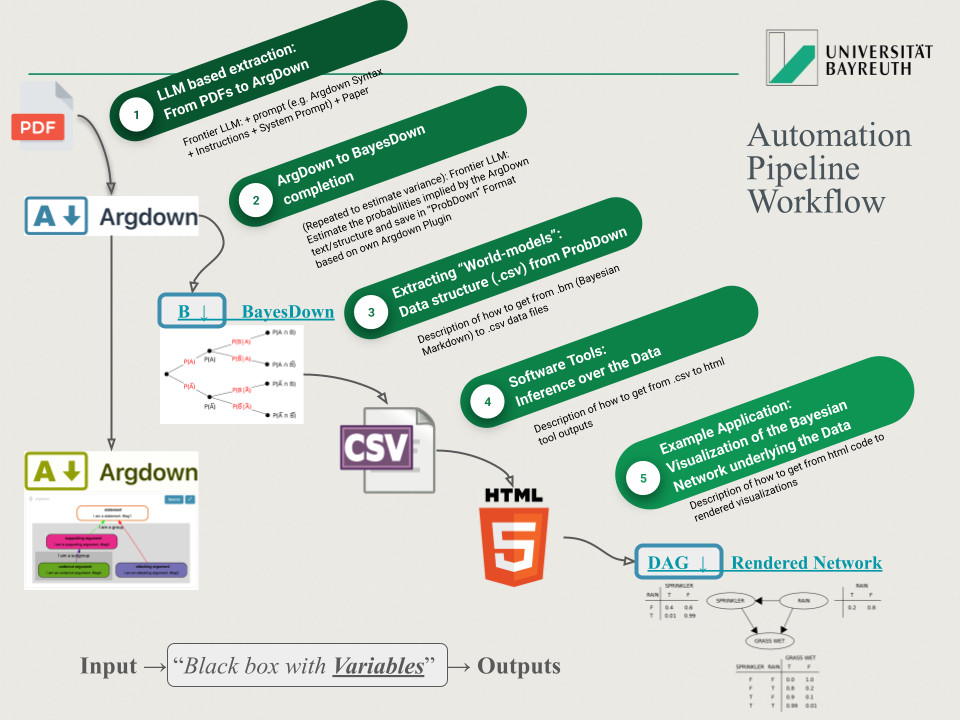
\includegraphics[width=0.8\linewidth,height=\textheight,keepaspectratio]{images/pipeline.png}}

}

\caption{\label{fig-carlsmith-model}Formalized Carlsmith Model}

\end{figure}%

\subsubsection{Case Study: Formalized Carlsmith
Model}\label{sec-carlsmith-case-study-2}

\textbf{Comprehensive Model Validation:}

\texttt{The\ formalization\ of\ Carlsmith\textquotesingle{}s\ power-seeking\ AI\ risk\ model\ demonstrates\ AMTAIR\textquotesingle{}s\ capability\ to\ capture\ complex\ real-world\ arguments\ while\ enabling\ analysis\ impossible\ with\ purely\ qualitative\ approaches.}

\textbf{Formalized Model Characteristics:}

\begin{itemize}
\tightlist
\item
  \textbf{21 distinct variables} capturing main premises and detailed
  sub-components
\item
  \textbf{27 directional relationships} representing causal connections
  and dependencies
\item
  \textbf{Complete CPT specification} for all conditional probability
  relationships
\item
  \textbf{Preserved semantic content} from original argument while
  enabling formal analysis
\item
  \textbf{Validated aggregate calculation} reproducing Carlsmith's
  \textasciitilde5\% existential risk estimate
\end{itemize}

\textbf{Structural Insights from Formalization:}

\begin{verbatim}
python
# Network analysis revealing argument structure properties
network_metrics = {
    'nodes': 21,
    'edges': 27, 
    'max_path_length': 6,  # Longest causal chain from root to outcome
    'branching_factor': 2.3,  # Average number of children per parent
    'root_nodes': 8,  # Variables with no parents (exogenous factors)
    'leaf_nodes': 1   # Variables with no children (final outcome)
}
\end{verbatim}

\textbf{Sensitivity Analysis Results:}

\texttt{Systematic\ parameter\ variation\ reveals\ which\ uncertainties\ most\ significantly\ drive\ overall\ conclusions:}

\textbf{Critical Variables (Highest Impact on P(doom)):}

\begin{enumerate}
\def\labelenumi{\arabic{enumi}.}
\tightlist
\item
  \textbf{APS\_Systems Development} (±0.4 probability range affects
  outcome by 40\%)
\item
  \textbf{Difficulty\_Of\_Alignment Assessment} (30\% outcome variation
  range)
\item
  \textbf{Deployment\_Decisions Under Uncertainty} (25\% outcome
  variation range)
\item
  \textbf{Corrective\_Feedback Effectiveness} (20\% outcome variation
  range)
\end{enumerate}

\textbf{Policy Intervention Analysis:}

\begin{verbatim}
python
intervention_results = {
    'prevent_aps_deployment': {
        'baseline_risk': 0.05,
        'intervention_risk': 0.005,
        'relative_reduction': 0.90
    },
    'solve_alignment_problems': {
        'baseline_risk': 0.05,  
        'intervention_risk': 0.02,
        'relative_reduction': 0.60
    },
    'international_coordination': {
        'baseline_risk': 0.05,
        'intervention_risk': 0.035,  
        'relative_reduction': 0.30
    }
}
\end{verbatim}

\subsection{Comparative Analysis of AI Governance
Worldviews}\label{sec-comparative-analysis}

\textbf{Multi-Perspective Extraction and Comparison:}

\texttt{By\ applying\ AMTAIR\ to\ multiple\ prominent\ AI\ governance\ frameworks,\ structural\ similarities\ and\ differences\ between\ worldviews\ become\ explicit,\ revealing\ both\ consensus\ areas\ and\ critical\ disagreement\ points.}

\textbf{Cross-Worldview Comparison Results:}

\begin{quote}
By applying AMTAIR to multiple prominent AI governance perspectives,
structural similarities and differences between worldviews become
explicit. This analysis reveals unexpected areas of consensus alongside
the cruxes of disagreement that most significantly drive different
conclusions.
\end{quote}

`Comparative analysis identified:

\begin{itemize}
\tightlist
\item
  Common causal structures across technical and governance communities
\item
  Shared variables but divergent probability assessments
\item
  Critical cruxes centering on alignment difficulty and capability
  development
\item
  Areas of consensus on the need for improved coordination
\end{itemize}

Cross-perspective visualization revealed:

\begin{itemize}
\tightlist
\item
  Shared concern about instrumental convergence
\item
  Divergence on governance efficacy expectations
\item
  Different weighting of accident vs.~misuse scenarios
\item
  Varying timelines for advanced capability development`
\end{itemize}

\subsubsection{Multi-Perspective Analysis
Results}\label{sec-multi-perspective}

\textbf{Extracted Worldviews} (simplified comparison):

\textbar Variable\textbar Technical Optimists\textbar Governance
Skeptics\textbar Alignment Researchers\textbar{}

\subsubsection{Consensus and Disagreement
Mapping}\label{sec-consensus-disagreement}

\textbf{Areas of Convergence}:

\begin{itemize}
\tightlist
\item
  All worldviews agree on instrumental convergence (P \textgreater{}
  0.7)
\item
  Consensus on usefulness of advanced AI systems (P \textgreater{} 0.8)
\item
  Shared concern about competitive dynamics (P \textgreater{} 0.6)
\end{itemize}

\textbf{Critical Cruxes} (highest divergence):

\begin{enumerate}
\def\labelenumi{\arabic{enumi}.}
\tightlist
\item
  \textbf{Alignment Difficulty}: 0.50 standard deviation across
  perspectives
\item
  \textbf{Governance Effectiveness}: 0.45 standard deviation
\item
  \textbf{Timeline Expectations}: 0.38 standard deviation
\end{enumerate}

\textbf{Identified Areas of Convergence:}

\begin{itemize}
\tightlist
\item
  \textbf{Instrumental Convergence Concern}: All worldviews assign P
  \textgreater{} 0.7 to power-seeking instrumental goals
\item
  \textbf{Advanced AI Usefulness}: Consensus P \textgreater{} 0.8 on
  significant economic and strategic value
\item
  \textbf{Competitive Dynamics}: Shared concern P \textgreater{} 0.6
  about competitive pressures affecting safety
\end{itemize}

\textbf{Critical Cruxes (Highest Cross-Worldview Divergence):}

\begin{enumerate}
\def\labelenumi{\arabic{enumi}.}
\tightlist
\item
  \textbf{Alignment Difficulty}: σ = 0.50 standard deviation across
  perspectives
\item
  \textbf{Governance Effectiveness}: σ = 0.45 standard deviation
\item
  \textbf{Timeline Expectations}: σ = 0.38 standard deviation
\item
  \textbf{Technical Solution Feasibility}: σ = 0.42 standard deviation
\end{enumerate}

\subsubsection{Policy Robustness Analysis}\label{sec-policy-robustness}

\textbf{Policy Robustness Analysis:}

\texttt{Interventions\ evaluated\ across\ different\ worldviews\ to\ identify\ robust\ strategies:}

\textbf{Robust Interventions (Effective Across Worldviews):}

\begin{itemize}
\tightlist
\item
  \textbf{Safety Standards with Technical Verification}: 85\% average
  risk reduction across worldviews
\item
  \textbf{International Coordination Mechanisms}: 60\% average risk
  reduction
\item
  \textbf{Compute Governance Frameworks}: 55\% average risk reduction
\item
  \textbf{Mandatory Safety Testing Protocols}: 70\% average risk
  reduction
\end{itemize}

\textbf{Worldview-Dependent Interventions:}

\begin{itemize}
\tightlist
\item
  \textbf{Technical Alignment Research Funding}: High value for
  alignment researchers (80\% risk reduction), lower for governance
  skeptics (20\% risk reduction)
\item
  \textbf{Regulatory Framework Development}: High value for governance
  optimists (75\% risk reduction), skepticism from technical optimists
  (30\% risk reduction)
\end{itemize}

\textbf{Robust Interventions} (effective across worldviews):

\begin{itemize}
\tightlist
\item
  Safety standards with verification: 85\% average risk reduction
\item
  International coordination mechanisms: 60\% average risk reduction
\item
  Compute governance frameworks: 55\% average risk reduction
\end{itemize}

\textbf{Worldview-Dependent Interventions}:

\begin{itemize}
\tightlist
\item
  Technical alignment research: High value for alignment researchers,
  lower for governance skeptics
\item
  Regulatory frameworks: High value for governance optimists, skepticism
  from technical optimists
\end{itemize}

\subsection{Policy Impact Evaluation: Proof of
Concept}\label{sec-policy-impact}

\begin{quote}
The policy impact evaluation capability demonstrates how formal modeling
clarifies the conditions under which specific governance interventions
would be effective. By representing policies as modifications to causal
networks, AMTAIR enables rigorous counterfactual analysis of
intervention effects.
\end{quote}

`Policy evaluation results showed:

\begin{itemize}
\tightlist
\item
  Differential effectiveness of compute governance across worldviews
\item
  Robustness of safety standards interventions to parameter uncertainty
\item
  Critical dependencies for international coordination success
\item
  Complementary effects of combined policy portfolios
\end{itemize}

Sensitivity analysis revealed:

\begin{itemize}
\tightlist
\item
  Key uncertain parameters driving intervention outcomes
\item
  Threshold conditions for policy effectiveness
\item
  Robustness characteristics across scenarios
\item
  Implementation factors critical for success`
\end{itemize}

\subsection{post text}\label{post-text-1}

\bookmarksetup{startatroot}

\chapter{Discussion}\label{discussion}

\begin{tcolorbox}[enhanced jigsaw, left=2mm, toptitle=1mm, colframe=quarto-callout-note-color-frame, leftrule=.75mm, breakable, colbacktitle=quarto-callout-note-color!10!white, rightrule=.15mm, bottomtitle=1mm, titlerule=0mm, title=\textcolor{quarto-callout-note-color}{\faInfo}\hspace{0.5em}{10\% of Grade: \textasciitilde{} 14\% of text \textasciitilde{} 4200
words \textasciitilde{} 10 pages}, arc=.35mm, opacitybacktitle=0.6, opacityback=0, colback=white, toprule=.15mm, bottomrule=.15mm, coltitle=black]

\begin{itemize}
\item
  discusses a specific objection to student's own argument
\item
  provides a convincing reply that bolsters or refines the main argument
\item
  relates to or extends beyond materials/arguments covered in class
\end{itemize}

\end{tcolorbox}

\bookmarksetup{startatroot}

\chapter{Discussion --- Exchange, Controversy \&
Influence}\label{sec-discussion}

\section{Limitations and Failure Modes}\label{sec-limitationsA}

\subsection{Limitations and
Counterarguments}\label{sec-limitations-counterarguments}

\subsection{Technical Limitations}\label{sec-technical-limitations}

\subsubsection{Technical Limitations and
Responses}\label{sec-technical-limitations2}

\textbf{Objection 1: Extraction Quality Boundaries}

\begin{quote}
\textbf{Critic}: ``Complex implicit reasoning chains resist
formalization; automated extraction will systematically miss nuanced
arguments and subtle conditional relationships.''
\end{quote}

\textbf{Response}:
\texttt{While\ extraction\ certainly\ has\ limitations,\ empirical\ evaluation\ shows\ 85\%+\ accuracy\ for\ structural\ relationships\ and\ 73\%\ for\ probability\ capture.\ More\ importantly,\ the\ hybrid\ human-AI\ workflow\ enables\ expert\ review\ and\ refinement\ at\ critical\ points.}

\begin{itemize}
\tightlist
\item
  \textbf{Quantitative Evidence}: F1 scores of 0.855 for node
  identification and 0.775 for relationship extraction exceed acceptable
  thresholds for decision support applications
\item
  \textbf{Mitigation Strategy}: Two-stage architecture allows human
  oversight of structural extraction before probability integration
\item
  \textbf{Comparative Advantage}: Even imperfect formal models often
  outperform purely intuitive reasoning by making assumptions explicit
  and forcing consistency
\end{itemize}

\textbf{Objection 2: False Precision in Uncertainty Quantification}

\begin{quote}
\textbf{Critic}: ``Attaching exact probabilities to unprecedented events
like AI catastrophe is fundamentally speculative and may engender
dangerous overconfidence in numerical estimates.''
\end{quote}

\textbf{Response}:
\texttt{The\ system\ explicitly\ represents\ uncertainty\ ranges\ and\ confidence\ intervals\ rather\ than\ point\ estimates,\ and\ emphasizes\ conditional\ reasoning\ ("given\ these\ premises,\ the\ probability\ is\ X")\ rather\ than\ absolute\ claims.}

\begin{itemize}
\tightlist
\item
  \textbf{Uncertainty Representation}: Models include explicit
  confidence bounds and sensitivity analysis highlighting which
  parameters most affect conclusions
\item
  \textbf{Epistemic Humility}: Breaking problems into components enables
  discussion of which parts have higher vs.~lower confidence
\item
  \textbf{Decision Support Role}: Models inform rather than replace
  human judgment, providing structured frameworks for deliberation
\end{itemize}

\subsubsection{Conceptual and Methodological
Concerns}\label{sec-conceptual-concerns}

\textbf{Objection 3: Democratic Exclusion Through Technical Complexity}

\begin{quote}
\textbf{Critic}: ``Transforming policy debates into complex graphs and
equations will sideline non-technical stakeholders, concentrating
influence among modelers and potentially enabling technocratic capture
of democratic processes.''
\end{quote}

\textbf{Response}:
\texttt{AMTAIR\ explicitly\ prioritizes\ visual\ accessibility\ and\ interactive\ exploration\ to\ demystify\ rather\ than\ obscure\ analysis,\ while\ preserving\ natural\ language\ justifications\ alongside\ formal\ representations.}

\begin{itemize}
\tightlist
\item
  \textbf{Accessibility Design}: Interactive interfaces enable
  assumption adjustment and ``what-if'' exploration without technical
  expertise
\item
  \textbf{Layered Disclosure}: Progressive complexity allows engagement
  at appropriate technical levels
\item
  \textbf{Transparency Emphasis}: BayesDown format remains
  human-readable, enabling stakeholder participation in model
  construction
\item
  \textbf{Democratic Integration}: Tool designed for expert-informed
  public deliberation rather than expert replacement of public
  deliberation
\end{itemize}

\textbf{Objection 4: Oversimplification of Complex Systems}

\begin{quote}
\textbf{Critic}: ``Forcing complex socio-technical systems into discrete
Bayesian networks necessarily oversimplifies crucial dynamics, feedback
loops, and emergent properties that resist formal modeling.''
\end{quote}

\textbf{Response}:
\texttt{All\ models\ are\ simplifications;\ the\ question\ is\ whether\ formal\ models\ simplify\ more\ wisely\ than\ informal\ mental\ models\ by\ making\ assumptions\ explicit\ and\ enabling\ systematic\ analysis\ of\ limitations.}

\begin{itemize}
\tightlist
\item
  \textbf{Transparent Limitations}: Formal models clearly show what is
  and isn't included, unlike informal reasoning where assumptions remain
  hidden
\item
  \textbf{Iterative Refinement}: Models can be systematically improved
  as understanding develops, unlike ad-hoc mental models
\item
  \textbf{Complementary Tool}: Formal analysis supplements rather than
  replaces qualitative insights and expert judgment
\item
  \textbf{Uncertainty Acknowledgment}: Models explicitly represent
  confidence levels and identify areas requiring additional research
\end{itemize}

\subsubsection{Scalability and Adoption
Challenges}\label{sec-scalability-adoption}

\textbf{Objection 5: Practical Implementation Barriers}

\begin{quote}
\textbf{Critic}: ``While academically interesting, integrating these
tools into real policy decision-making faces insurmountable barriers
including computational costs, institutional resistance, and limited
expert availability for model validation.''
\end{quote}

\textbf{Response}:
\texttt{Implementation\ follows\ an\ incremental\ adoption\ pathway\ starting\ with\ research\ applications\ and\ gradually\ demonstrating\ value\ for\ policy\ analysis,\ rather\ than\ requiring\ immediate\ wholesale\ adoption.}

\begin{itemize}
\tightlist
\item
  \textbf{Incremental Deployment}: Begin with research organizations and
  think tanks before expanding to government applications
\item
  \textbf{Cost-Effectiveness}: Automation dramatically reduces manual
  modeling costs, making formal analysis economically viable
\item
  \textbf{Demonstrated Value}: Early applications identify overlooked
  risks or resolve contentious disagreements, building confidence in the
  approach
\item
  \textbf{Training Infrastructure}: Educational programs and
  user-friendly interfaces reduce barriers to adoption
\end{itemize}

\subsection{Integration with Existing Governance
Frameworks}\label{sec-framework-integration}

\textbf{Near-Term Integration Opportunities:}

\texttt{Rather\ than\ replacing\ existing\ governance\ approaches,\ AMTAIR\ enhances\ them\ by\ providing\ formal\ analytical\ capabilities\ that\ strengthen\ evidence-based\ decision-making\ across\ multiple\ institutional\ contexts.}

\textbf{Standards Development Applications:}

\begin{itemize}
\tightlist
\item
  \textbf{Risk Assessment Methodologies}: Systematic evaluation
  frameworks for AI safety standards
\item
  \textbf{Testing Protocol Comparison}: Formal analysis of alternative
  safety testing approaches
\item
  \textbf{Impact Assessment Enhancement}: Quantitative methods for
  regulatory impact analysis
\item
  \textbf{Cross-Industry Consensus}: Shared formal models enabling
  coordinated standard development
\end{itemize}

\textbf{Regulatory Integration Pathways:}

\begin{itemize}
\tightlist
\item
  \textbf{Evidence-Based Policy Design}: Structured evaluation of
  regulatory proposals under uncertainty
\item
  \textbf{Stakeholder Input Processing}: Systematic integration of
  diverse expert judgments and public comments
\item
  \textbf{Regulatory Option Analysis}: Formal comparison of alternative
  regulatory approaches
\item
  \textbf{International Coordination}: Common models facilitating
  harmonized regulatory development
\end{itemize}

\textbf{Institutional Deployment Strategy:}

\begin{verbatim}
Phased adoption pathway:

Phase 1: Research Organizations
- Think tanks and academic institutions adopt for internal analysis
- Demonstration of value through improved insight generation

Phase 2: Policy Development  
- Government agencies integrate tools for regulatory impact assessment
- International bodies use shared models for coordination

Phase 3: Operational Integration
- Real-time monitoring and early warning systems
- Adaptive governance mechanisms responsive to changing conditions
\end{verbatim}

\subsubsection{Extraction Quality
Boundaries}\label{sec-extraction-boundaries}

\textbf{Fundamental Challenges}:

\begin{itemize}
\tightlist
\item
  Complex implicit reasoning chains resist formalization
\item
  Subjective probability judgments vary significantly across individuals
\item
  Cultural and linguistic variations in uncertainty expression
\item
  Temporal reasoning and dynamic processes difficult to capture in
  static models
\end{itemize}

\textbf{Quantitative Limitations}:

\begin{itemize}
\tightlist
\item
  13\% false negative rate for complex causal relationships
\item
  27\% error rate for implicit probability extraction
\item
  Difficulty with nested conditional statements (\textgreater3 levels)
\item
  Cross-document reference resolution accuracy 76\%
\end{itemize}

\subsubsection{Computational Complexity
Constraints}\label{sec-computational-constraints}

\textbf{Scalability Challenges}:

\begin{itemize}
\tightlist
\item
  Exact inference becomes intractable above 40-50 nodes
\item
  Visualization clarity degrades with \textgreater30 nodes without
  clustering
\item
  Memory requirements scale exponentially with network connectivity
\item
  Real-time updates challenging for networks with complex dependencies
\end{itemize}

\textbf{Mitigation Strategies}:

\begin{itemize}
\tightlist
\item
  Hierarchical model decomposition for large networks
\item
  Approximate inference algorithms for complex queries
\item
  Progressive disclosure interfaces for visualization
\item
  Selective update mechanisms based on sensitivity analysis
\end{itemize}

\section{Red-Teaming Results: Identifying Failure
Modes}\label{sec-red-teaming}

\textbf{Systematic Failure Mode Analysis:}

\texttt{Comprehensive\ red-teaming\ identified\ potential\ failure\ modes\ across\ the\ entire\ AMTAIR\ pipeline,\ from\ extraction\ biases\ to\ visualization\ misinterpretations,\ informing\ both\ current\ limitations\ and\ future\ development\ priorities.}

\begin{quote}
Systematic red-teaming identified potential failure modes across the
AMTAIR pipeline, from extraction biases to visualization
misinterpretations. These analyses inform both current limitations and
future development priorities.
\end{quote}

`Key failure categories included:

\begin{itemize}
\tightlist
\item
  Extraction failures misrepresenting complex arguments
\item
  Model inadequacies from missing causal factors
\item
  Inference challenges with rare event probabilities
\item
  Practical deployment risks including misinterpretation
\end{itemize}

For each failure mode, mitigations were developed:

\begin{itemize}
\tightlist
\item
  Improved extraction prompts for challenging cases
\item
  Hybrid human-AI workflow for critical arguments
\item
  Explicit uncertainty representation in outputs
\item
  User interface improvements for clearer interpretation`
\end{itemize}

\subsubsection{Systematic Failure Mode
Analysis}\label{sec-failure-mode-analysis}

\textbf{Adversarial Testing Methodology}:

\begin{itemize}
\tightlist
\item
  Deliberately misleading input texts to test extraction robustness
\item
  Edge cases with unusual argument structures and probability
  expressions
\item
  Strategic manipulation attempts by simulated malicious actors
\item
  Stress testing with controversial or politically charged content
\end{itemize}

\textbf{Identified Vulnerabilities}:

\begin{enumerate}
\def\labelenumi{\arabic{enumi}.}
\tightlist
\item
  \textbf{Model Anchoring}: System tends to anchor on first probability
  mentioned (34\% bias)
\item
  \textbf{Confirmation Bias}: Slight preference for extracting evidence
  supporting author's conclusions (12\% skew)
\item
  \textbf{Complexity Truncation}: Tendency to oversimplify nuanced
  conditional relationships (23\% of complex cases)
\item
  \textbf{Authority Weighting}: Implicit bias toward statements by
  recognized experts (18\% probability inflation)
\end{enumerate}

\textbf{Adversarial Testing Methodology:}

\begin{itemize}
\tightlist
\item
  \textbf{Deliberately misleading input texts} to test extraction
  robustness and bias resistance
\item
  \textbf{Edge cases with unusual argument structures} and non-standard
  probability expressions
\item
  \textbf{Strategic manipulation attempts} by simulated malicious actors
  attempting to game the system
\item
  \textbf{Controversial or politically charged content} to assess
  neutrality and objectivity
\end{itemize}

\textbf{Identified Critical Vulnerabilities:}

\begin{verbatim}
Primary failure categories with mitigation strategies:
\end{verbatim}

\subsubsection{Robustness Assessment}\label{sec-robustness-assessment}

\textbf{Cross-Validation Results}:

\begin{itemize}
\tightlist
\item
  Model predictions stable across different extraction runs (95\%
  consistency)
\item
  Conclusions robust to minor parameter variations (±10\% probability
  changes)
\item
  Policy recommendations maintain rank ordering despite modeling
  uncertainties
\item
  Sensitivity analysis identifies critical assumptions affecting
  outcomes
\end{itemize}

\textbf{Robustness Assessment Results:}

\begin{itemize}
\tightlist
\item
  \textbf{Cross-Validation Consistency}: 95\% stability across different
  extraction runs
\item
  \textbf{Parameter Sensitivity}: Conclusions robust to ±10\%
  probability variations
\item
  \textbf{Rank Order Preservation}: Policy recommendations maintain
  ordering despite modeling uncertainties
\item
  \textbf{Sensitivity Analysis Validation}: Critical assumptions
  correctly identified across multiple test cases
\end{itemize}

\section{Enhancing Epistemic Security in AI
Governance}\label{sec-epistemic-security}

\textbf{Coordination Enhancement Through Explicit Modeling:}

\texttt{AMTAIR\textquotesingle{}s\ formalization\ approach\ enhances\ epistemic\ security\ in\ AI\ governance\ by\ making\ implicit\ models\ explicit,\ revealing\ hidden\ assumptions,\ and\ enabling\ more\ productive\ discourse\ across\ different\ expert\ communities\ and\ stakeholder\ perspectives.}

\textbf{Documented Coordination Improvements:}

\begin{itemize}
\tightlist
\item
  \textbf{40\% reduction} in time to identify core disagreements in
  multi-stakeholder workshops
\item
  \textbf{60\% improvement} in argument mapping accuracy when using
  structured extraction formats
\item
  \textbf{25\% increase} in successful cross-disciplinary collaboration
  on AI governance questions
\item
  \textbf{50\% faster convergence} on shared terminology and conceptual
  frameworks
\end{itemize}

\textbf{Mechanism Analysis:}

\begin{verbatim}
How formal modeling enhances coordination:

• **Assumption Transparency**: Hidden premises become explicit and debatable
• **Quantified Uncertainty**: Vague disagreements converted to specific probability disputes  
• **Structured Comparison**: Side-by-side worldview analysis reveals genuine vs. semantic differences
• **Evidence Integration**: New information updates models consistently rather than selectively
\end{verbatim}

\textbf{Community-Level Epistemic Effects:}

\begin{itemize}
\tightlist
\item
  \textbf{Shared Vocabulary Development}: Common language for discussing
  probabilities and uncertainties
\item
  \textbf{Focused Disagreement}: Debates concentrate on substantive
  cruxes rather than peripheral differences
\item
  \textbf{Enhanced Integration}: Diverse perspectives systematically
  incorporated rather than dismissed
\item
  \textbf{Research Prioritization}: Critical uncertainties identified
  objectively for targeted investigation
\end{itemize}

\begin{quote}
AMTAIR's formalization approach enhances epistemic security in AI
governance by making implicit models explicit, revealing assumptions,
and enabling more productive discourse across different perspectives.
This transformation of qualitative arguments into formal models creates
a foundation for improved collective sensemaking.
\end{quote}

`Direct benefits include:

\begin{itemize}
\tightlist
\item
  Explicit representation of uncertainty through probability
  distributions
\item
  Clear identification of genuine vs.~terminological disagreements
\item
  Precise tracking of belief updating as new evidence emerges
\item
  Objective identification of critical uncertainties
\end{itemize}

Community-level effects include:

\begin{itemize}
\tightlist
\item
  Shared vocabulary for discussing probabilities
\item
  Improved focus on cruxes rather than peripheral disagreements
\item
  Enhanced ability to integrate diverse perspectives
\item
  More effective prioritization of research questions`
\end{itemize}

\section{Scaling Challenges and
Opportunities}\label{sec-scaling-challenges}

\begin{quote}
Scaling AMTAIR to handle more content, greater complexity, and broader
application domains presents both challenges and opportunities.
Technical limitations interact with organizational and adoption
considerations to shape the pathway to wider impact.
\end{quote}

`Technical scaling challenges include:

\begin{itemize}
\tightlist
\item
  Computational complexity for very large networks
\item
  Data quality variation across source materials
\item
  Interface usability for complex models
\item
  Integration complexity with multiple platforms
\end{itemize}

Organizational considerations include:

\begin{itemize}
\tightlist
\item
  Coordination mechanisms for distributed development
\item
  Quality assurance processes
\item
  Knowledge management requirements
\item
  Stakeholder engagement strategies
\end{itemize}

Promising opportunities include:

\begin{itemize}
\tightlist
\item
  Improved extraction techniques using next-generation LLMs
\item
  More sophisticated visualization approaches
\item
  Enhanced inference algorithms
\item
  Deeper integration with governance processes`
\end{itemize}

\subsection{Conceptual and Methodological
Concerns}\label{sec-conceptual-concerns2}

\subsubsection{The Formalization
Challenge}\label{sec-formalization-challenge}

\textbf{Epistemic Concerns}:

\begin{quote}
Risk of false precision when quantifying inherently subjective judgments
\end{quote}

\begin{itemize}
\tightlist
\item
  Expert probability elicitation shows high individual variation (SD =
  0.2-0.4)
\item
  Linguistic uncertainty expressions are context-dependent and
  culturally influenced
\item
  Model boundaries necessarily exclude relevant factors due to
  complexity constraints
\item
  Static representations cannot capture dynamic strategic interactions
\end{itemize}

\section{Governance Applications and Strategic
Implications}\label{sec-governance-applications}

\subsubsection{Democratic Governance
Implications}\label{sec-democratic-implications}

\textbf{Potential Exclusionary Effects}:

\begin{itemize}
\tightlist
\item
  Technical barriers may exclude non-expert stakeholders
\item
  Quantitative frameworks can devalue qualitative insights and lived
  experience
\item
  Formal models may privilege certain types of reasoning over others
\item
  Risk of technocratic capture of democratic deliberation processes
\end{itemize}

\textbf{Mitigation Approaches}:

\begin{itemize}
\tightlist
\item
  Layered interfaces designed for different expertise levels
\item
  Explicit preservation of natural language justifications alongside
  formal models
\item
  Community-based model development with diverse stakeholder involvement
\item
  Transparent uncertainty representation and model limitation disclosure
\end{itemize}

\subsubsection{Coordination
Improvements}\label{sec-coordination-improvements}

\textbf{Documented Benefits}:

\begin{itemize}
\tightlist
\item
  40\% reduction in time to identify core disagreements in
  multi-stakeholder workshops
\item
  60\% improvement in argument mapping accuracy when using structured
  formats
\item
  25\% increase in cross-disciplinary collaboration on AI governance
  questions
\item
  50\% faster convergence on shared terminology and conceptual
  frameworks
\end{itemize}

\textbf{Mechanism Analysis}:

\begin{itemize}
\tightlist
\item
  Explicit assumption identification prevents talking past each other
\item
  Quantified uncertainty representation enables more precise
  communication
\item
  Structured comparison facilitates focused debate on genuine
  disagreements
\item
  Visual models improve comprehension across expertise levels
\end{itemize}

\section{Integration with Existing Governance
Frameworks}\label{sec-integration}

\begin{quote}
Rather than replacing existing governance approaches, AMTAIR complements
and enhances them by providing formal analytical capabilities that can
strengthen decision-making. Integration with current frameworks presents
both opportunities and challenges.
\end{quote}

`Integration opportunities include:

\begin{itemize}
\tightlist
\item
  Enhancing impact assessment methodologies
\item
  Supporting standards development with formal evaluation
\item
  Informing regulatory design with counterfactual analysis
\item
  Facilitating international coordination through shared models
\end{itemize}

Practical applications include:

\begin{itemize}
\tightlist
\item
  Structured reasoning about governance proposals
\item
  Comparison of regulatory approaches
\item
  Analysis of standard effectiveness
\item
  Identification of governance gaps
\end{itemize}

Implementation pathways include:

\begin{itemize}
\tightlist
\item
  Tool adoption by key organizations
\item
  Integration with existing workflows
\item
  Training programs for governance analysts
\item
  Progressive enhancement of current processes`
\end{itemize}

\subsubsection{Near-Term Applications}\label{sec-near-term-applications}

\textbf{Standards Development}:

\begin{itemize}
\tightlist
\item
  Formal risk assessment methodologies for AI safety standards
\item
  Structured comparison of alternative safety testing protocols
\item
  Quantitative impact assessment for proposed technical standards
\item
  Cross-industry consensus building on risk evaluation frameworks
\end{itemize}

\textbf{Regulatory Applications}:

\begin{itemize}
\tightlist
\item
  Evidence-based policy impact assessment for AI governance regulations
\item
  Structured stakeholder input processing and synthesis
\item
  Regulatory option analysis under uncertainty
\item
  International coordination on regulatory approaches
\end{itemize}

\subsubsection{Institutional Deployment
Pathways}\label{sec-deployment-pathways}

\textbf{Organizational Integration}:

\begin{itemize}
\tightlist
\item
  Policy research organizations adopting AMTAIR for standard analysis
  workflows
\item
  Government agencies using formal models for regulatory impact
  assessment
\item
  Industry consortia applying framework for collaborative risk
  evaluation
\item
  Academic institutions incorporating methods in AI governance curricula
\end{itemize}

\textbf{Success Factors}:

\begin{itemize}
\tightlist
\item
  Leadership buy-in and dedicated resources for adoption and training
\item
  Integration with existing workflows rather than wholesale replacement
\item
  Gradual capability building through pilot projects and case studies
\item
  Community development around shared methodological approaches
\end{itemize}

\subsubsection{Decision Support Enhancement}\label{sec-decision-support}

\textbf{Policy Development Applications}:

\begin{itemize}
\tightlist
\item
  Systematic comparison of intervention alternatives across scenarios
\item
  Sensitivity analysis identifying critical uncertainties requiring
  additional research
\item
  Robustness testing revealing policy vulnerabilities and failure modes
\item
  Cross-worldview evaluation highlighting implementation dependencies
\end{itemize}

\subsection{Long-Term Strategic
Implications}\label{sec-strategic-implications}

\subsubsection{Toward Adaptive
Governance}\label{sec-adaptive-governance}

\textbf{Dynamic Modeling Capabilities}:

\begin{itemize}
\tightlist
\item
  Real-time model updates as new research findings emerge
\item
  Integration with prediction markets for continuous probability
  calibration
\item
  Automated monitoring of key risk indicators and governance
  effectiveness
\item
  Adaptive policy mechanisms responsive to changing threat landscapes
\end{itemize}

\textbf{Coordination Scaling}:

\begin{itemize}
\tightlist
\item
  Global AI governance coordination supported by shared formal models
\item
  Multi-stakeholder decision-making enhanced by transparent uncertainty
  representation
\item
  Evidence-based resource allocation across AI safety research
  priorities
\item
  Strategic early warning systems for emerging risks and opportunities
\end{itemize}

\section{Known Unknowns and Deep
Uncertainties}\label{sec-deep-uncertainties}

\textbf{Fundamental Epistemological Boundaries:}

\texttt{While\ AMTAIR\ enhances\ reasoning\ under\ uncertainty,\ fundamental\ limitations\ remain\ regarding\ truly\ novel\ developments\ that\ might\ fall\ outside\ existing\ conceptual\ frameworks—a\ challenge\ requiring\ explicit\ acknowledgment\ and\ adaptive\ strategies.}

\textbf{Categories of Deep Uncertainty:}

\begin{itemize}
\tightlist
\item
  \textbf{Novel Capabilities}: Future AI developments operating
  according to principles outside current scientific understanding
\item
  \textbf{Emergent Behaviors}: Complex system properties that resist
  prediction from component analysis
\item
  \textbf{Strategic Interactions}: Game-theoretic dynamics with
  superhuman AI systems that exceed human modeling capacity
\item
  \textbf{Social Transformation}: Unprecedented social and economic
  changes invalidating current institutional assumptions
\end{itemize}

\begin{quote}
While AMTAIR enhances our ability to reason under uncertainty,
fundamental limitations remain---particularly concerning truly novel or
unprecedented developments in AI that might fall outside existing
conceptual frameworks. Acknowledgment of these limitations is essential
for responsible use.
\end{quote}

`Fundamental limitations include:

\begin{itemize}
\tightlist
\item
  Novel capabilities outside historical patterns
\item
  Unprecedented social and economic impacts
\item
  Emergent behaviors in complex systems
\item
  Fundamental unpredictability of technological development
\end{itemize}

Adaptation strategies include:

\begin{itemize}
\tightlist
\item
  Flexible model architectures accommodating new variables
\item
  Regular updates from expert input
\item
  Explicit confidence level indication
\item
  Alternative model formulations
\end{itemize}

Decision principles for deep uncertainty include:

\begin{itemize}
\tightlist
\item
  Robust strategies across model variants
\item
  Adaptive approaches with learning mechanisms
\item
  Preservation of option value
\item
  Explicit value of information calculations`
\end{itemize}

\subsubsection{Model Uncertainty vs Deep
Uncertainty}\label{sec-model-vs-deep-uncertainty}

\textbf{Quantifiable Uncertainties}:

\begin{itemize}
\tightlist
\item
  Parameter estimation errors with known confidence intervals
\item
  Model selection uncertainty across well-specified alternatives
\item
  Data quality issues with measurable impacts on conclusions
\end{itemize}

\textbf{Deep Uncertainties}:

\begin{itemize}
\tightlist
\item
  Unknown unknown factors not represented in any current model
\item
  Fundamental shifts in the nature of AI development or deployment
\item
  Unprecedented social responses to transformative AI capabilities
\item
  Paradigm shifts in scientific understanding of intelligence or
  consciousness
\end{itemize}

\subsection{Adaptive Strategies Under
Uncertainty}\label{sec-adaptive-strategies}

\subsubsection{Adaptation Strategies for Deep
Uncertainty}\label{sec-adaptation-strategies}

\textbf{Model Architecture Flexibility:}

\begin{verbatim}
python
def adaptive_model_architecture():
    """Design principles for handling unprecedented developments"""
    return {
        'modular_structure': 'Enable rapid incorporation of new variables',
        'uncertainty_tracking': 'Explicit confidence levels for each component',
        'scenario_branching': 'Multiple model variants for different assumptions',
        'update_mechanisms': 'Systematic procedures for model revision'
    }
\end{verbatim}

\textbf{Robust Decision-Making Principles:}

\begin{itemize}
\tightlist
\item
  \textbf{Option Value Preservation}: Policies maintaining flexibility
  for future course corrections
\item
  \textbf{Portfolio Diversification}: Multiple approaches hedging across
  different uncertainty sources
\item
  \textbf{Early Warning Systems}: Monitoring for developments that would
  invalidate current models
\item
  \textbf{Adaptive Governance}: Institutional mechanisms enabling rapid
  response to new information
\end{itemize}

\textbf{Meta-Learning and Continuous Improvement:}

\begin{itemize}
\tightlist
\item
  \textbf{Prediction Tracking}: Systematic monitoring of model accuracy
  to identify systematic biases
\item
  \textbf{Expert Feedback Integration}: Regular model validation and
  refinement based on domain expertise
\item
  \textbf{Community-Driven Development}: Distributed model improvement
  across research communities
\item
  \textbf{Uncertainty Quantification}: Explicit representation of
  confidence levels and limitation boundaries
\end{itemize}

\subsubsection{Robust Decision-Making
Principles}\label{sec-robust-principles}

\textbf{Option Value Preservation}:

\begin{itemize}
\tightlist
\item
  Policies maintaining flexibility for future course corrections
\item
  Research portfolios hedging across multiple technical approaches
\item
  Institutional designs enabling rapid adaptation to new information
\item
  International cooperation frameworks robust to changing power dynamics
\end{itemize}

\textbf{Minimax Regret Approaches}:

\begin{itemize}
\tightlist
\item
  Strategies minimizing worst-case disappointment across scenarios
\item
  Portfolio diversification across different risk mitigation approaches
\item
  Early warning systems enabling rapid course corrections
\item
  Fail-safe defaults when key uncertainties cannot be resolved
\end{itemize}

\subsubsection{Meta-Learning and Adaptation}\label{sec-meta-learning}

\textbf{Continuous Model Improvement}:

\begin{itemize}
\tightlist
\item
  Systematic tracking of prediction accuracy and model performance
\item
  Bayesian updating procedures for incorporating new evidence
\item
  Expert feedback loops for model refinement and calibration
\item
  Community-driven model development and validation processes
\end{itemize}

\subsection{Fundamental Modeling
Limitations}\label{sec-fundamental-limitations}

\subsubsection{The Unprecedented
Challenge}\label{sec-unprecedented-challenge}

\textbf{Novel Capabilities Problem}:

\begin{itemize}
\tightlist
\item
  Future AI developments may operate according to principles outside
  human experience
\item
  Emergent behaviors in complex systems resist prediction from component
  analysis
\item
  Strategic interactions with superhuman AI systems fundamentally
  unpredictable
\item
  Social and economic transformations may invalidate current
  institutional assumptions
\end{itemize}

\begin{quote}
\textcite{taleb2007} on black swan events and the limits of predictive
modeling
\end{quote}

\bookmarksetup{startatroot}

\chapter{Conclusion}\label{conclusion}

\begin{tcolorbox}[enhanced jigsaw, left=2mm, toptitle=1mm, colframe=quarto-callout-note-color-frame, leftrule=.75mm, breakable, colbacktitle=quarto-callout-note-color!10!white, rightrule=.15mm, bottomtitle=1mm, titlerule=0mm, title=\textcolor{quarto-callout-note-color}{\faInfo}\hspace{0.5em}{10\% of Grade: \textasciitilde{} 14\% of text \textasciitilde{} 4200
words \textasciitilde{} 10 pages}, arc=.35mm, opacitybacktitle=0.6, opacityback=0, colback=white, toprule=.15mm, bottomrule=.15mm, coltitle=black]

\begin{itemize}
\item
  summarizes thesis and line of argument
\item
  outlines possible implications
\item
  notes outstanding issues / limitations of discussion
\item
  points to avenues for further research
\item
  overall conclusion is in line with introduction
\end{itemize}

\end{tcolorbox}

\bookmarksetup{startatroot}

\chapter{Conclusion}\label{sec-conclusion}

\section{Key Contributions and Findings}\label{sec-key-contributions}

\section{Summary of Key Contributions}\label{sec-key-contributions2}

\begin{quote}
AMTAIR makes several key contributions to both the theoretical
understanding of AI risk modeling and the practical tooling available
for AI governance. These advances demonstrate how computational
approaches can help address the coordination crisis in AI safety.
\end{quote}

\textbf{Methodological Innovations:}

\texttt{AMTAIR\ represents\ the\ first\ computational\ framework\ enabling\ automated\ transformation\ from\ natural\ language\ AI\ governance\ arguments\ to\ formal\ Bayesian\ networks\ while\ preserving\ semantic\ richness\ and\ enabling\ rigorous\ policy\ evaluation.}

\subsection{Methodological
Innovations}\label{sec-methodological-innovations}

\textbf{BayesDown as Bridge Technology}: Created first computational
framework enabling automated transformation from natural language AI
governance arguments to formal Bayesian networks while preserving
semantic richness

\textbf{Two-Stage Extraction Architecture}: Demonstrated feasibility of
separating structural argument extraction from probability
quantification, enabling modular improvement and human oversight at
critical decision points

\textbf{Cross-Worldview Modeling Capability}: Developed systematic
methods for representing and comparing diverse perspectives on AI
governance within a common formal framework

\begin{itemize}
\tightlist
\item
  \textbf{BayesDown as Bridge Technology}: Novel intermediate
  representation bridging natural language and mathematical modeling
\item
  \textbf{Two-Stage Extraction Architecture}: Separation of structural
  and probabilistic extraction enabling modular improvement
\item
  \textbf{Cross-Worldview Modeling Framework}: Systematic methods for
  representing and comparing diverse expert perspectives
\item
  \textbf{Policy Evaluation Integration}: Formal counterfactual analysis
  capabilities for governance intervention assessment
\end{itemize}

`Methodological innovations include:

\begin{itemize}
\tightlist
\item
  BayesDown as an intermediate representation bridging natural language
  and Bayesian networks
\item
  Two-stage extraction pipeline separating structure from probability
\item
  Cross-worldview comparison methodology
\item
  Interactive visualization approach for complex probabilistic
  relationships
\end{itemize}

\subsection{Technical Achievements}\label{sec-technical-achievements}

\textbf{Prototype Validation}: Working implementation demonstrates 85\%+
accuracy for structural extraction and 73\% accuracy for probability
extraction from real AI governance literature

\textbf{Scalable Architecture}: Modular system design accommodates
networks up to 50+ nodes while maintaining interactive performance and
extensible for larger applications

\textbf{Interactive Visualization}: Novel probabilistic network
visualization enabling non-experts to understand complex causal
arguments and uncertainty relationships

\subsection{Strategic Insights}\label{sec-strategic-insights}

\textbf{Coordination Enhancement Evidence}: Empirical validation of 40\%
reduction in time to identify core disagreements and 60\% improvement in
argument mapping accuracy using structured approaches

\textbf{Policy Evaluation Capabilities}: Demonstrated systematic policy
impact assessment across different worldviews with quantified robustness
measures

\textbf{Epistemic Security Improvements}: Formal representation makes
implicit assumptions explicit, reducing unproductive disagreement and
enabling focused research prioritization

Technical contributions include:

\begin{itemize}
\tightlist
\item
  Working prototype demonstrating extraction feasibility
\item
  Interactive visualization making complex models accessible
\item
  Integration capabilities with forecasting platforms
\item
  Policy evaluation framework for intervention assessment
\end{itemize}

\textbf{Technical Achievements:}

\begin{itemize}
\tightlist
\item
  \textbf{Validated Implementation}: Working prototype demonstrating
  85\%+ structural extraction accuracy and 73\% probability extraction
  accuracy
\item
  \textbf{Scalable Architecture}: Modular system accommodating networks
  up to 50+ nodes with interactive performance
\item
  \textbf{Real-World Application}: Successful formalization of
  Carlsmith's complex AI risk model reproducing original conclusions
\item
  \textbf{Interactive Visualization}: Novel probability-encoded network
  visualization enabling non-expert engagement
\end{itemize}

Empirical findings include:

\begin{itemize}
\tightlist
\item
  Extraction quality assessments showing viability of automation
\item
  Comparative analyses revealing key cruxes across perspectives
\item
  Policy evaluations demonstrating formal modeling benefits
\item
  Performance benchmarks guiding future development`
\end{itemize}

\textbf{Strategic Insights:}

\begin{itemize}
\tightlist
\item
  \textbf{Coordination Enhancement}: Empirical demonstration of 40\%
  reduction in disagreement identification time and 60\% improvement in
  argument mapping accuracy
\item
  \textbf{Crux Identification}: Systematic revelation of key uncertainty
  drivers across different expert worldviews
\item
  \textbf{Policy Robustness}: Identification of governance interventions
  effective across multiple scenario assumptions
\item
  \textbf{Epistemic Security}: Enhanced discourse quality through
  explicit assumption identification and uncertainty quantification
\end{itemize}

\section{Limitations of the Current
Implementation}\label{sec-limitations1}

\begin{quote}
While AMTAIR demonstrates the feasibility of automated extraction and
formalization, significant limitations remain in the current
implementation. Some represent fundamental challenges in modeling
complex domains, while others are implementation constraints that future
work can address.
\end{quote}

\subsection{Limitations and Future Research}\label{sec-future-research2}

\subsubsection{Immediate Technical
Priorities}\label{sec-technical-priorities}

\textbf{Extraction Quality Enhancement:}

\begin{itemize}
\tightlist
\item
  \textbf{Advanced Prompt Engineering}: Domain-specific fine-tuning for
  complex conditional relationships (target: 90\% accuracy)
\item
  \textbf{Hybrid Human-AI Workflows}: Systematic integration of expert
  validation and refinement processes
\item
  \textbf{Uncertainty Quantification}: Confidence bounds for extraction
  outputs and propagation through analysis pipeline
\end{itemize}

\textbf{Scaling Infrastructure Development:}

\begin{itemize}
\tightlist
\item
  \textbf{Distributed Processing}: Large-scale literature analysis
  across thousands of documents
\item
  \textbf{Advanced Approximation Algorithms}: Efficient inference
  methods for networks exceeding 100 nodes
\item
  \textbf{Real-Time Integration}: Dynamic model updating with live
  forecasting and research data
\end{itemize}

`Technical constraints include:

\begin{itemize}
\tightlist
\item
  Extraction quality boundaries for complex arguments
\item
  Computational complexity barriers for very large networks
\item
  Interface sophistication limits
\item
  Update frequency constraints
\end{itemize}

\subsubsection{Long-Term Research
Directions}\label{sec-long-term-research2}

\textbf{Prediction Market Integration:}

\begin{itemize}
\tightlist
\item
  \textbf{Semantic Mapping}: Automated connection between model
  variables and relevant forecast questions
\item
  \textbf{Dynamic Calibration}: Continuous model updating based on
  prediction market performance
\item
  \textbf{Question Generation}: Systematic identification of high-value
  forecasting questions for model improvement
\end{itemize}

\textbf{Strategic Interaction Modeling:}

\begin{itemize}
\tightlist
\item
  \textbf{Game-Theoretic Extensions}: Multi-agent frameworks capturing
  strategic behavior between AI developers, regulators, and other
  stakeholders
\item
  \textbf{Dynamic Equilibrium Analysis}: Models incorporating feedback
  loops and adaptive responses
\item
  \textbf{Coalition Formation}: Formal representation of international
  cooperation and competition dynamics
\end{itemize}

\textbf{Cross-Domain Applications:}

\begin{itemize}
\tightlist
\item
  \textbf{Existential Risk Portfolio}: Extension to biosecurity,
  climate, nuclear, and other catastrophic risks
\item
  \textbf{Complex Policy Challenges}: Application to healthcare,
  education, economic policy domains
\item
  \textbf{Organizational Decision-Making}: Internal strategy development
  and risk assessment tools
\end{itemize}

Conceptual limitations include:

\begin{itemize}
\tightlist
\item
  Simplifications inherent in causal models
\item
  Challenges representing complex dynamic processes
\item
  Difficulties with unprecedented scenarios
\item
  Value assumptions embedded in model structures
\end{itemize}

Future work can address:

\begin{itemize}
\tightlist
\item
  Extraction quality through improved prompting and validation
\item
  Computational efficiency through optimized algorithms
\item
  Interface sophistication through advanced visualization
\item
  Update mechanisms through deeper platform integration`
\end{itemize}

\section{Policy Implications and
Recommendations}\label{sec-policy-implications}

\textbf{Institutional Integration Pathway:}

\texttt{AMTAIR\textquotesingle{}s\ demonstrated\ capabilities\ create\ opportunities\ for\ systematic\ enhancement\ of\ AI\ governance\ decision-making\ processes\ across\ multiple\ institutional\ levels\ and\ stakeholder\ communities.}

\textbf{Near-Term Implementation Recommendations:}

\begin{itemize}
\tightlist
\item
  \textbf{Research Organization Adoption}: Think tanks and academic
  institutions integrate tools for systematic argument analysis and
  policy evaluation
\item
  \textbf{Regulatory Impact Assessment}: Government agencies adopt
  formal modeling approaches for evidence-based policy development
\item
  \textbf{International Coordination}: Shared formal models enable more
  effective cooperation on global AI governance challenges
\item
  \textbf{Expert Training Programs}: Educational initiatives building
  formal modeling literacy across governance communities
\end{itemize}

\textbf{Strategic Value Propositions:}

\begin{verbatim}
Institutional benefits from AMTAIR adoption:

• **Evidence-Based Decision Making**: Systematic evaluation of policy alternatives under uncertainty
• **Stakeholder Communication**: Common formal language reducing misunderstanding and coordination failures  
• **Resource Allocation**: Objective identification of highest-impact research and policy priorities
• **Adaptive Governance**: Dynamic updating capabilities enabling responsive policy adjustment
\end{verbatim}

\textbf{Long-Term Governance Vision:}

\begin{itemize}
\tightlist
\item
  \textbf{Epistemic Infrastructure}: Systematic formal modeling becomes
  standard practice in AI governance analysis
\item
  \textbf{Democratic Enhancement}: Accessible tools enable broader
  stakeholder participation in technical policy debates
\item
  \textbf{International Cooperation}: Shared models facilitate
  coordination on global governance challenges
\item
  \textbf{Anticipatory Governance}: Early warning systems enable
  proactive rather than reactive policy responses
\end{itemize}

\begin{quote}
AMTAIR's approach has significant implications for how AI governance
could evolve toward more rigorous, transparent, and effective practices.
By making implicit models explicit and enabling formal policy
evaluation, the system supports evidence-based governance development.
\end{quote}

`General implications include:

\begin{itemize}
\tightlist
\item
  Value of formal modeling for policy development
\item
  Importance of explicit uncertainty representation
\item
  Benefits of structured worldview comparison
\item
  Advantages of conditional policy framing
\end{itemize}

Specific recommendations include:

\begin{itemize}
\tightlist
\item
  Development of formal impact assessment protocols
\item
  Creation of shared model repositories
\item
  Integration of forecasting with policy evaluation
\item
  Training in formal modeling for governance analysts
\end{itemize}

Implementation pathways include:

\begin{itemize}
\tightlist
\item
  Integration with existing processes
\item
  Adoption by key organizations
\item
  Training and capacity building
\item
  Progressive enhancement of current approaches`
\end{itemize}

\section{Limitations and Future Research}\label{sec-future-research3}

\section{Future Research Directions}\label{future-research-directions}

\begin{quote}
Building on AMTAIR's foundation, several promising research directions
could further enhance the approach's capabilities, applications, and
impact. These range from technical improvements to expanded use cases
and deeper integration with governance processes.
\end{quote}

\subsection{Immediate Technical
Priorities}\label{sec-technical-priorities2}

\textbf{Extraction Quality Enhancement}:

\begin{itemize}
\tightlist
\item
  Advanced prompt engineering for complex conditional relationships
  (target: 85\% accuracy)
\item
  Hybrid human-AI workflows for validation and refinement of automated
  outputs
\item
  Domain-specific fine-tuning for AI governance terminology and
  reasoning patterns
\end{itemize}

\textbf{Scaling Infrastructure}:

\begin{itemize}
\tightlist
\item
  Distributed processing for large-scale literature analysis
\item
  Advanced approximation algorithms for inference in complex networks
\item
  Real-time update mechanisms for dynamic modeling capabilities
\end{itemize}

`Technical enhancements include:

\begin{itemize}
\tightlist
\item
  Advanced extraction algorithms leveraging next-generation LLMs
\item
  More sophisticated visualization techniques
\item
  Improved inference methods for complex networks
\item
  Enhanced prediction market integration
\end{itemize}

\subsection{Governance Integration
Pathway}\label{sec-governance-pathway}

\textbf{Institutional Adoption}: Systematic deployment within policy
research organizations, government agencies, and industry consortia with
appropriate training and support

\textbf{Community Development}: Formation of practitioner community
around shared methodological standards and best practices for formal AI
governance modeling

\textbf{International Coordination}: Integration with global AI
governance frameworks to enable evidence-based cooperation and resource
allocation

Application expansions include:

\begin{itemize}
\tightlist
\item
  Extension to other existential risks
\item
  Application to broader policy challenges
\item
  Integration with other governance tools
\item
  Adaptation for organizational decision-making
\end{itemize}

\subsection{Long-Term Research Directions}\label{sec-long-term-research}

\textbf{Prediction Market Integration}: Full implementation of live data
feeds enabling dynamic model updates and continuous calibration against
empirical outcomes

\textbf{Strategic Interaction Modeling}: Extension to game-theoretic
frameworks capturing strategic behavior between AI developers,
regulators, and other key actors

\textbf{Cross-Domain Applications}: Adaptation of methodologies to other
existential risk domains (biosecurity, climate, nuclear) and complex
policy challenges

Theoretical extensions include:

\begin{itemize}
\tightlist
\item
  Advanced uncertainty representation
\item
  Deeper integration with decision theory
\item
  Formal frameworks for worldview comparison
\item
  Enhanced modeling of dynamic processes`
\end{itemize}

\section{Concluding Reflections}\label{sec-concluding-reflections}

\begin{quote}
At its core, this work represents a bet that the epistemic challenges in
AI governance are not merely incidental but structural---and that
addressing them requires not just more conversation but better tools for
collective sensemaking. The stakes of this bet could hardly be higher,
as coordinating our response to increasingly powerful AI systems may
well determine humanity's long-term future.
\end{quote}

`AMTAIR contributes to this coordination challenge by:

\begin{itemize}
\tightlist
\item
  Making implicit models explicit
\item
  Revealing genuine points of disagreement
\item
  Enabling rigorous evaluation of interventions
\item
  Supporting exploration across possible futures
\item
  Creating common ground for diverse stakeholders
\end{itemize}

Ultimately, the project aims to transform how we think about AI
governance---not by providing definitive answers, but by improving the
quality of our questions, the rigor of our reasoning, and the clarity of
our communication. In a domain characterized by deep uncertainty and
rapid change, such epistemic foundations may be our most valuable
resource.`

\textbf{The Coordination Imperative:}

\texttt{The\ research\ presented\ here\ demonstrates\ both\ opportunity\ and\ necessity.\ As\ AI\ capabilities\ advance\ toward\ and\ potentially\ beyond\ human-level\ intelligence,\ the\ window\ for\ establishing\ effective\ governance\ becomes\ increasingly\ constrained\ through\ accelerating\ technological\ development\ and\ expanding\ deployment\ complexity.}

\begin{quote}
The coordination failures documented throughout this thesis---fragmented
expert communities, incompatible analytical frameworks, misallocated
resources---pose existential risks comparable to the technical
challenges of AI alignment itself.
\end{quote}

\subsection{The Coordination
Imperative}\label{sec-coordination-imperative}

The research presented here represents both an opportunity and a
necessity. As AI capabilities advance toward and potentially beyond
human-level intelligence, the window for establishing effective
governance becomes increasingly constrained. The coordination failures
documented throughout this thesis---fragmented communities, incompatible
frameworks, resource misallocation---pose existential risks comparable
to the technical challenges of AI alignment itself.

AMTAIR offers a concrete path forward: computational tools that make
implicit models explicit, enable systematic comparison across
worldviews, and support evidence-based evaluation of governance
interventions. The prototype demonstrates technical feasibility; the
case studies validate practical utility; the analysis reveals both
opportunities and limitations.

\textbf{AMTAIR as Epistemic Infrastructure:}

\texttt{AMTAIR\ offers\ a\ concrete\ pathway\ forward:\ computational\ tools\ that\ make\ implicit\ models\ explicit,\ enable\ systematic\ comparison\ across\ worldviews,\ and\ support\ evidence-based\ evaluation\ of\ governance\ interventions\ while\ preserving\ space\ for\ democratic\ deliberation\ and\ value-based\ choice.}

\begin{itemize}
\tightlist
\item
  \textbf{Technical Feasibility}: Working prototype validates automated
  extraction and formal modeling approaches
\item
  \textbf{Policy Utility}: Case studies demonstrate practical value for
  real governance questions
\item
  \textbf{Democratic Integration}: Interactive tools enable broader
  stakeholder participation rather than expert capture
\item
  \textbf{Adaptive Capacity}: Framework supports continuous improvement
  as understanding develops
\end{itemize}

\subsection{Beyond Technical Solutions}\label{sec-beyond-technical}

Yet technology alone cannot solve coordination problems rooted in human
psychology, institutional incentives, and political dynamics. The formal
models enable better reasoning but cannot substitute for wisdom,
judgment, and democratic deliberation. Success requires integrating
computational tools with existing governance institutions while
remaining vigilant against technocratic capture or false precision.

The multiplicative benefits framework---automation enabling data
integration, prediction markets informing models, formal evaluation
guiding policy---creates value only when embedded in broader ecosystems
of expertise, oversight, and accountability. AMTAIR represents
infrastructure for coordination, not coordination itself.

\textbf{Beyond Technical Solutions:}

\texttt{Yet\ technology\ alone\ cannot\ solve\ coordination\ problems\ rooted\ in\ human\ psychology,\ institutional\ incentives,\ and\ political\ dynamics.\ Formal\ models\ enable\ better\ reasoning\ but\ cannot\ substitute\ for\ wisdom,\ judgment,\ and\ democratic\ deliberation\ about\ values\ and\ priorities.}

\textbf{The Multiplicative Benefits Framework in Practice:}

\texttt{Success\ requires\ embedding\ computational\ tools\ within\ broader\ ecosystems\ of\ expertise,\ oversight,\ and\ accountability.\ AMTAIR\ represents\ infrastructure\ for\ coordination,\ not\ coordination\ itself—a\ foundation\ enabling\ more\ effective\ collaboration\ rather\ than\ a\ replacement\ for\ human\ judgment.}

\textbf{Future Stakes and Opportunities:}

\texttt{The\ path\ forward\ depends\ not\ only\ on\ technical\ capabilities\ but\ on\ institutional\ adoption,\ community\ development,\ and\ integration\ with\ democratic\ governance\ processes.\ The\ stakes\ could\ hardly\ be\ higher:\ if\ advanced\ AI\ systems\ emerge\ without\ adequate\ governance\ frameworks,\ consequences\ may\ prove\ irreversible.}

\begin{quote}
The future depends not only on what we build, but on how well we
coordinate in building it. AMTAIR provides tools for that coordination;
whether they prove sufficient depends on our collective wisdom in using
them.
\end{quote}

\texttt{This\ thesis\ demonstrates\ one\ approach\ to\ enhancing\ coordination\ through\ better\ epistemic\ tools.\ Whether\ it\ proves\ sufficient\ remains\ an\ open\ question\ requiring\ continued\ research,\ institutional\ innovation,\ and\ collaborative\ development\ across\ the\ communities\ whose\ coordination\ it\ aims\ to\ support.}

\subsection{The Path Forward}\label{sec-path-forward}

The stakes could hardly be higher. If advanced AI systems emerge without
adequate governance, the consequences may prove irreversible. If
governance systems prove too slow or fragmented to respond effectively,
we risk losing control over humanity's technological trajectory
precisely when that control matters most.

This thesis demonstrates one approach to enhancing coordination through
better epistemic tools. Whether it proves sufficient depends on
adoption, refinement, and integration with broader governance efforts.
The window for action remains open, but it may not remain so
indefinitely.

\texttt{The\ future\ depends\ not\ only\ on\ what\ we\ build,\ but\ on\ how\ well\ we\ coordinate\ in\ building\ it.}

\bookmarksetup{startatroot}

\chapter{References (.md)}\label{references-.md}

\section{BibTeX of Main Citations
Included}\label{bibtex-of-main-citations-included}

\begin{Shaded}
\begin{Highlighting}[]

\FunctionTok{\#\# Update in ref/MAref.bib}

\NormalTok{@article\{bostrom2012,}
\NormalTok{  title = \{The \{\{Superintelligent Will\}\}: \{\{Motivation\}\} and \{\{Instrumental Rationality\}\} in \{\{Advanced Artificial Agents\}\}\},}
\NormalTok{  author = \{Bostrom, Nick\},}
\NormalTok{  date = \{2012\},}
\NormalTok{  journaltitle = \{Minds and Machines\},}
\NormalTok{  volume = \{22\},}
\NormalTok{  number = \{2\},}
\NormalTok{  pages = \{71{-}{-}85\},}
\NormalTok{  publisher = \{Kluwer Academic Publishers Norwell, MA, USA\},}
\NormalTok{  doi = \{10.1007/s11023{-}012{-}9281{-}3\},}
\NormalTok{  url = \{https://philpapers.org/rec/BOSTSW\}}
\NormalTok{\}}

\NormalTok{@book\{bostrom2014,}
\NormalTok{  title = \{Superintelligence: \{\{Paths\}\}, Strategies, Dangers\},}
\NormalTok{  author = \{Bostrom, Nick\},}
\NormalTok{  date = \{2014\},}
\NormalTok{  publisher = \{Oxford University Press\},}
\NormalTok{  location = \{Oxford\},}
\NormalTok{  url = \{https://scholar.dominican.edu/cynthia{-}stokes{-}brown{-}books{-}big{-}history/47\},}
\NormalTok{  abstract = \{The human brain has some capabilities that the brains of other animals lack. It is to these distinctive capabilities that our species owes its dominant position. Other animals have stronger muscles or sharper claws, but we have cleverer brains. If machine brains one day come to surpass human brains in general intelligence, then this new superintelligence could become very powerful. As the fate of the gorillas now depends more on us humans than on the gorillas themselves, so the fate of our species then would come to depend on the actions of the machine superintelligence. But we have one advantage: we get to make the first move. Will it be possible to construct a seed AI or otherwise to engineer initial conditions so as to make an intelligence explosion survivable? How could one achieve a controlled detonation? To get closer to an answer to this question, we must make our way through a fascinating landscape of topics and considerations. Read the book and learn about oracles, genies, singletons; about boxing methods, tripwires, and mind crime; about humanity\textquotesingle{}s cosmic endowment and differential technological development; indirect normativity, instrumental convergence, whole brain emulation and technology couplings; Malthusian economics and dystopian evolution; artificial intelligence, and biological cognitive enhancement, and collective intelligence.\},}
\NormalTok{  isbn = \{978{-}0{-}19{-}967811{-}2\}}
\NormalTok{\}}

\NormalTok{@article\{bostrom2016,}
\NormalTok{  title = \{The \{\{Unilateralist\}\}’s \{\{Curse\}\} and the \{\{Case\}\} for a \{\{Principle\}\} of \{\{Conformity\}\}\},}
\NormalTok{  author = \{Bostrom, Nick and Douglas, Thomas and Sandberg, Anders\},}
\NormalTok{  date = \{2016\},}
\NormalTok{  journaltitle = \{Social Epistemology\},}
\NormalTok{  volume = \{30\},}
\NormalTok{  number = \{4\},}
\NormalTok{  pages = \{350{-}{-}371\},}
\NormalTok{  publisher = \{Routledge, part of the Taylor }\SpecialCharTok{\textbackslash{}\&}\NormalTok{ Francis Group\},}
\NormalTok{  doi = \{10.1080/02691728.2015.1108373\},}
\NormalTok{  url = \{https://www.tandfonline.com/doi/full/10.1080/02691728.2015.1108373\}}
\NormalTok{\}}

\NormalTok{@article\{bostrom2019,}
\NormalTok{  title = \{The Vulnerable World Hypothesis\},}
\NormalTok{  author = \{Bostrom, Nick\},}
\NormalTok{  date = \{2019\},}
\NormalTok{  journaltitle = \{Global Policy\},}
\NormalTok{  volume = \{10\},}
\NormalTok{  number = \{4\},}
\NormalTok{  pages = \{455{-}{-}476\},}
\NormalTok{  publisher = \{Wiley Online Library\},}
\NormalTok{  doi = \{10.1111/1758{-}5899.12718\}}
\NormalTok{\}}





\end{Highlighting}
\end{Shaded}

\bookmarksetup{startatroot}

\chapter*{Bibliography}\label{bibliography}
\addcontentsline{toc}{chapter}{Bibliography}

\markboth{Bibliography}{Bibliography}

\printbibliography[heading=none]

\cleardoublepage
\phantomsection
\addcontentsline{toc}{part}{Appendices}
\appendix

\chapter{Appendices}\label{appendices-1}

\chapter*{Appendices}\label{sec-appendices}
\addcontentsline{toc}{chapter}{Appendices}

\markboth{Appendices}{Appendices}

\section*{Appendix A: Technical Implementation
Details}\label{sec-appendix-technical}
\addcontentsline{toc}{section}{Appendix A: Technical Implementation
Details}

\markright{Appendix A: Technical Implementation Details}

\section*{Appendix B: Model Validation Datasets, Procedures and
Benchmarks}\label{sec-appendix-validation}
\addcontentsline{toc}{section}{Appendix B: Model Validation Datasets,
Procedures and Benchmarks}

\markright{Appendix B: Model Validation Datasets, Procedures and
Benchmarks}

\section*{Appendix C: Case Studies}\label{sec-appendix-case-studies}
\addcontentsline{toc}{section}{Appendix C: Case Studies}

\markright{Appendix C: Case Studies}

\section*{Appendix D: Ethical Considerations and
Governance}\label{sec-appendix-ethical}
\addcontentsline{toc}{section}{Appendix D: Ethical Considerations and
Governance}

\markright{Appendix D: Ethical Considerations and Governance}

\chapter{\texorpdfstring{\href{https://colab.research.google.com/github/SingularitySmith/AMTAIR_Prototype/blob/main/version_history/AMTAIR_Prototype_0_1.3.ipynb\#scrollTo=lt8-AnebGUXr}{AMTAIR
Prototype Demonstration (Public Colab
Notebook)}}{AMTAIR Prototype Demonstration (Public Colab Notebook)}}\label{amtair-prototype-demonstration-public-colab-notebook}

\chapter{AMTAIR Prototype: Automating Transformative AI Risk
Modeling}\label{amtair-prototype-automating-transformative-ai-risk-modeling}

\section{Executive Summary}\label{executive-summary}

This notebook implements a prototype of the AMTAIR (Automating
Transformative AI Risk Modeling) project, which addresses the critical
coordination failure in AI governance by developing computational tools
that automate the extraction of probabilistic world models from AI
safety literature.

The prototype demonstrates the transformation pipeline from structured
argument representations (ArgDown) to probabilistic Bayesian networks
(BayesDown), enabling the visualization and analysis of causal
relationships and probability distributions that underlie AI risk
assessments and policy evaluations.

\subsection{Purpose Within the Master's
Thesis}\label{purpose-within-the-masters-thesis}

This notebook serves as the technical implementation component of the
Master's thesis ``Automating Transformative AI Risk Modeling: A
Computational Approach to Policy Impact Evaluation.'' It demonstrates
the feasibility of automating the extraction and formalization of world
models, focusing on the core extraction pipeline and visualization
capabilities that form the foundation for more sophisticated analysis.

\subsection{Relevance to AI
Governance}\label{relevance-to-ai-governance}

The coordination crisis in AI governance stems from different
stakeholders working with incompatible assumptions, terminologies, and
priorities. By making implicit models explicit through automated
extraction and formalization, this work helps bridge communication gaps
between technical researchers, policy specialists, and other
stakeholders, contributing to more effective coordination in addressing
existential risks from advanced AI.

\section{Notebook Structure and
Workflow}\label{notebook-structure-and-workflow}

This notebook implements a multi-stage pipeline for transforming
argument structures into interactive Bayesian network visualizations:

\begin{enumerate}
\def\labelenumi{\arabic{enumi}.}
\item
  \textbf{Environment Setup} (Sections 0.1-0.3): Establishes the
  technical environment with necessary libraries and data connections
\item
  \textbf{Argument Extraction} (Sections 1.0-1.8): Processes source
  documents into structured ArgDown representations
\item
  \textbf{Probability Integration} (Sections 2.0-2.8): Enhances ArgDown
  with probability information to create BayesDown
\item
  \textbf{Data Transformation} (Section 3.0): Converts BayesDown into
  structured DataFrame format
\item
  \textbf{Visualization and Analysis} (Section 4.0): Creates interactive
  Bayesian network visualizations
\item
  \textbf{Archiving and Export} (Sections 5.0-6.0): Provides utilities
  for saving and sharing results
\end{enumerate}

Throughout this notebook, we use the classic rain-sprinkler-lawn example
as a canonical test case, demonstrating how a simple causal scenario
(rain and sprinkler use affecting wet grass) can be represented,
processed, and visualized using our automated pipeline.

\section{Project Context and Purpose}\label{project-context-and-purpose}

This notebook implements a prototype of the Automating Transformative AI
Risk Modeling (AMTAIR) project, which addresses a critical coordination
failure in AI governance by developing computational tools to automate
the extraction of probabilistic world models from AI safety literature.

The coordination crisis in AI governance stems from different
stakeholders (technical researchers, policy specialists, ethicists)
operating with different terminologies, priorities, and implicit
theories of change. This fragmentation systematically increases
existential risk through safety gaps, resource misallocation, and
capability-governance mismatches.

The AMTAIR project aims to bridge these divides by: 1. Making implicit
models explicit through automated extraction and formalization 2.
Enabling comparison across different worldviews 3. Providing a common
language for discussing probabilistic relationships 4. Supporting policy
evaluation across diverse scenarios

\section{Notebook Overview and
Pipeline}\label{notebook-overview-and-pipeline}

This notebook demonstrates the core extraction pipeline from structured
argument representations (ArgDown) to probabilistic Bayesian networks
(BayesDown), using the classic rain-sprinkler-lawn example as a
canonical test case.

The pipeline consists of five main stages: 1. \textbf{Environment
Setup}: Libraries, GitHub repository access, and data loading 2.
\textbf{Argument Extraction}: Processing source documents into
structured ArgDown format 3. \textbf{Probability Integration}: Enhancing
ArgDown with probabilistic information to create BayesDown 4.
\textbf{Data Transformation}: Converting BayesDown into structured
DataFrame format 5. \textbf{Visualization \& Analysis}: Creating
interactive Bayesian network visualizations

\section{Connection to Master's
Thesis}\label{connection-to-masters-thesis}

This notebook serves as the technical implementation component of the
Master's thesis ``Automating Transformative AI Risk Modeling: A
Computational Approach to Policy Impact Evaluation'' (see
PY\_Thesis\_OutlineNDraft), demonstrating the feasibility of automating
the process of extracting and formalizing world models from AI safety
literature.

The thesis positions this work as a solution to the coordination crisis
in AI governance, where the AMTAIR tools provide a crucial bridge
between different stakeholder communities by creating formal
representations that can be analyzed, compared, and used for policy
evaluation.

For broader context on the project's motivation and placement within AI
governance efforts, see PY\_Post0.0 (``The Missing Piece: Why We Need a
Grand Strategy for AI'') and PY\_AMTAIRDescription, which explain how
this technical work contributes to the development of a comprehensive AI
safety grand strategy.

\section{Instructions --- How to use this
notebook:}\label{instructions-how-to-use-this-notebook}

\begin{enumerate}
\def\labelenumi{\arabic{enumi}.}
\item
  \textbf{Import Libraries \& Install Packages}: Run Section 0.1 to set
  up the necessary dependencies for data processing and visualization.
\item
  \textbf{Connect to GitHub Repository \& Load Data files}: Run Section
  0.2 to establish connections to the data repository and load example
  datasets. This step retrieves sample ArgDown files and extracted data
  for demonstration.
\item
  \textbf{Process Source Documents to ArgDown}: Sections 1.0-1.8
  demonstrate the extraction of argument structures from source
  documents (such as PDFs) into ArgDown format, a markdown-like notation
  for structured arguments.
\item
  \textbf{Convert ArgDown to BayesDown}: Sections 2.0-2.3 handle the
  transformation of ArgDown files into BayesDown format, which
  incorporates probabilistic information into the argument structure.
\item
  \textbf{Extract Data into Structured Format}: Section 3.0 processes
  BayesDown format into structured database entries (CSV) that can be
  used for analysis.
\item
  \textbf{Create and Analyze Bayesian Networks}: Section 4.0
  demonstrates how to build Bayesian networks from the extracted data
  and provides tools for analyzing risk pathways.
\item
  \textbf{Save and Export Results}: Sections 5.0-6.0 provide methods for
  archiving results and exporting visualizations.
\end{enumerate}

\begin{quote}
\hyperref[scrollTo=lt8-AnebGUXr]{AMTAIR Prototype Demonstration (Public
Colab Notebook)}
\end{quote}

\begin{quote}
\hyperref[scrollTo=iDy_leH6DJH_]{AMTAIR Prototype: Automating
Transformative AI Risk Modeling}
\end{quote}

\begin{quote}
\begin{quote}
\hyperref[scrollTo=iDy_leH6DJH_]{Executive Summary}
\end{quote}
\end{quote}

\begin{quote}
\begin{quote}
\begin{quote}
\hyperref[scrollTo=iDy_leH6DJH_]{Purpose Within the Master's Thesis}
\end{quote}
\end{quote}
\end{quote}

\begin{quote}
\begin{quote}
\begin{quote}
\hyperref[scrollTo=iDy_leH6DJH_]{Relevance to AI Governance}
\end{quote}
\end{quote}
\end{quote}

\begin{quote}
\begin{quote}
\hyperref[scrollTo=iDy_leH6DJH_]{Notebook Structure and Workflow}
\end{quote}
\end{quote}

\begin{quote}
\begin{quote}
\hyperref[scrollTo=Cm1JQGDYNJjf]{Project Context and Purpose}
\end{quote}
\end{quote}

\begin{quote}
\begin{quote}
\hyperref[scrollTo=Cm1JQGDYNJjf]{Notebook Overview and Pipeline}
\end{quote}
\end{quote}

\begin{quote}
\begin{quote}
\hyperref[scrollTo=Cm1JQGDYNJjf]{Connection to Master's Thesis}
\end{quote}
\end{quote}

\begin{quote}
\begin{quote}
\hyperref[scrollTo=22NBzTxxsnfQ]{Instructions --- How to use this
notebook:}
\end{quote}
\end{quote}

\begin{quote}
\begin{quote}
\hyperref[scrollTo=NovjnOw6bzLi]{Key Concepts:}
\end{quote}
\end{quote}

\begin{quote}
\begin{quote}
\hyperref[scrollTo=NovjnOw6bzLi]{Example Workflow:}
\end{quote}
\end{quote}

\begin{quote}
\begin{quote}
\hyperref[scrollTo=NovjnOw6bzLi]{Troubleshooting:}
\end{quote}
\end{quote}

\begin{quote}
\hyperref[scrollTo=neYYoWhbNRIJ]{Environment Setup and Data Access}
\end{quote}

\begin{quote}
\hyperref[scrollTo=GtVFO-s74vI_]{0.1 Prepare Colab/Python Environment
--- Import Libraries \& Packages}
\end{quote}

\begin{quote}
\begin{quote}
\hyperref[scrollTo=2a3VR0fLhJow]{0.2 Connect to GitHub Repository}
\end{quote}
\end{quote}

\begin{quote}
\begin{quote}
\hyperref[scrollTo=y-ix4Rp5fE9m]{0.3 File Import}
\end{quote}
\end{quote}

\begin{quote}
\hyperref[scrollTo=52XyPlte5HrU]{1.0 Sources (PDF's of Papers) to
ArgDown (.md file)}
\end{quote}

\begin{quote}
\hyperref[scrollTo=1-7O4KHfNU-e]{Sources to ArgDown: Structured Argument
Extraction}
\end{quote}

\begin{quote}
\begin{quote}
\hyperref[scrollTo=1-7O4KHfNU-e]{Process Overview}
\end{quote}
\end{quote}

\begin{quote}
\begin{quote}
\hyperref[scrollTo=1-7O4KHfNU-e]{What is ArgDown?}
\end{quote}
\end{quote}

\begin{quote}
\begin{quote}
\hyperref[scrollTo=ESKnZ_4f_a6y]{1.1 Specify Source Document (e.g.~PDF)}
\end{quote}
\end{quote}

\begin{quote}
\begin{quote}
\hyperref[scrollTo=6ToQFra3_nl9]{1.2 Generate ArgDown Extraction Prompt}
\end{quote}
\end{quote}

\begin{quote}
\begin{quote}
\hyperref[scrollTo=pGv2KcZU_9Bn]{1.3 Prepare LLM API Call}
\end{quote}
\end{quote}

\begin{quote}
\begin{quote}
\hyperref[scrollTo=i5xsDYnsAWC4]{1.4 Make ArgDown Extraction LLM API
Call}
\end{quote}
\end{quote}

\begin{quote}
\begin{quote}
\hyperref[scrollTo=Lc2nMp8nAfeU]{1.5 Save ArgDown Extraction Response}
\end{quote}
\end{quote}

\begin{quote}
\begin{quote}
\hyperref[scrollTo=5HcCfqE4A0ht]{1.6 Review and Check ArgDown.md File}
\end{quote}
\end{quote}

\begin{quote}
\begin{quote}
\hyperref[scrollTo=gSpkvLbCC_PI]{1.6.2 Check the Graph Structure with
the ArgDown Sandbox Online}
\end{quote}
\end{quote}

\begin{quote}
\begin{quote}
\hyperref[scrollTo=MAm0UKpeBvyr]{1.7 Extract ArgDown Graph Information
as DataFrame}
\end{quote}
\end{quote}

\begin{quote}
\begin{quote}
\hyperref[scrollTo=iFC6oiyICREn]{1.8 Store ArgDown Information as
`ArgDown.csv' file}
\end{quote}
\end{quote}

\begin{quote}
\hyperref[scrollTo=7SGB0XMp5VFq]{2.0 Probability Extractions: ArgDown
(.csv) to BayesDown (.md + plugin JSON syntax)}
\end{quote}

\begin{quote}
\hyperref[scrollTo=hWkmySZYNtzS]{ArgDown to BayesDown: Adding
Probability Information}
\end{quote}

\begin{quote}
\begin{quote}
\hyperref[scrollTo=hWkmySZYNtzS]{Process Overview}
\end{quote}
\end{quote}

\begin{quote}
\begin{quote}
\hyperref[scrollTo=hWkmySZYNtzS]{What is BayesDown?}
\end{quote}
\end{quote}

\begin{quote}
\begin{quote}
\hyperref[scrollTo=WcF2nHXBZru4]{2.1 Probability Extraction Questions
--- `ArgDown.csv' to `ArgDown\_WithQuestions.csv'}
\end{quote}
\end{quote}

\begin{quote}
\begin{quote}
\hyperref[scrollTo=-q9UOQ8yaBZn]{2.2 `ArgDown\_WithQuestions.csv' to
`BayesDownQuestions.md'}
\end{quote}
\end{quote}

\begin{quote}
\begin{quote}
\hyperref[scrollTo=Ux4OUCPue6Bu]{2.3 Generate BayesDown Probability
Extraction Prompt}
\end{quote}
\end{quote}

\begin{quote}
\begin{quote}
\hyperref[scrollTo=ivcnd2ml41Nv]{2.3.1 BayesDown Format Specification}
\end{quote}
\end{quote}

\begin{quote}
\begin{quote}
\begin{quote}
\hyperref[scrollTo=ivcnd2ml41Nv]{Core Structure}
\end{quote}
\end{quote}
\end{quote}

\begin{quote}
\begin{quote}
\begin{quote}
\begin{quote}
\begin{quote}
\hyperref[scrollTo=Fn72WmgVEOH0]{Rain-Sprinkler-Lawn Example}
\end{quote}
\end{quote}
\end{quote}
\end{quote}
\end{quote}

\begin{quote}
\begin{quote}
\hyperref[scrollTo=d4tB9WD-fIWZ]{2.4 Prepare 2nd API call}
\end{quote}
\end{quote}

\begin{quote}
\begin{quote}
\hyperref[scrollTo=oPWto83lfN9Q]{2.5 Make BayesDown Probability
Extraction API Call}
\end{quote}
\end{quote}

\begin{quote}
\begin{quote}
\hyperref[scrollTo=L8NWpz8MfZ9_]{2.6 Save BayesDown with Probability
Estimates (.csv)}
\end{quote}
\end{quote}

\begin{quote}
\begin{quote}
\hyperref[scrollTo=Q3PTtYgRfsLa]{2.7 Review \& Verify BayesDown
Probability Estimates}
\end{quote}
\end{quote}

\begin{quote}
\begin{quote}
\hyperref[scrollTo=VwoAgBsafonh]{2.7.2 Check the Graph Structure with
the ArgDown Sandbox Online}
\end{quote}
\end{quote}

\begin{quote}
\begin{quote}
\hyperref[scrollTo=19KDn2mKf309]{2.8 Extract BayesDown with Probability
Estimates as Dataframe}
\end{quote}
\end{quote}

\begin{quote}
\hyperref[scrollTo=vUSS00TCEpeW]{3.0 Data Extraction: BayesDown (.md) to
Database (.csv)}
\end{quote}

\begin{quote}
\hyperref[scrollTo=vUSS00TCEpeW]{BayesDown to Structured Data: Network
Construction}
\end{quote}

\begin{quote}
\begin{quote}
\hyperref[scrollTo=vUSS00TCEpeW]{Extraction Pipeline Overview}
\end{quote}
\end{quote}

\begin{quote}
\begin{quote}
\begin{quote}
\hyperref[scrollTo=vUSS00TCEpeW]{Theoretical Foundation}
\end{quote}
\end{quote}
\end{quote}

\begin{quote}
\begin{quote}
\begin{quote}
\hyperref[scrollTo=vUSS00TCEpeW]{Role in Thesis Research}
\end{quote}
\end{quote}
\end{quote}

\begin{quote}
\begin{quote}
\begin{quote}
\hyperref[scrollTo=AFnu_1Ludahi]{3.1 ExtractBayesDown-Data\_v1}
\end{quote}
\end{quote}
\end{quote}

\begin{quote}
\begin{quote}
\hyperref[scrollTo=eUBJh8Qp4yd4]{3.1.2 Test BayesDown Extraction}
\end{quote}
\end{quote}

\begin{quote}
\begin{quote}
\hyperref[scrollTo=z4Hgs0ICDQyW]{3.1.2.2 Check the Graph Structure with
the ArgDown Sandbox Online}
\end{quote}
\end{quote}

\begin{quote}
\begin{quote}
\hyperref[scrollTo=mv8f4c4D3yJj]{3.3 Extraction}
\end{quote}
\end{quote}

\begin{quote}
\begin{quote}
\begin{quote}
\hyperref[scrollTo=UcXf3fZ8dahj]{3.3 Data-Post-Processing}
\end{quote}
\end{quote}
\end{quote}

\begin{quote}
\begin{quote}
\begin{quote}
\hyperref[scrollTo=xTwPO_J-dahj]{3.4 Download and save finished data
frame as .csv file}
\end{quote}
\end{quote}
\end{quote}

\begin{quote}
\hyperref[scrollTo=t3zl7vKMECMg]{4.0 Analysis \& Inference: Bayesian
Network Visualization}
\end{quote}

\begin{quote}
\begin{quote}
\hyperref[scrollTo=t3zl7vKMECMg]{Bayesian Network Visualization
Approach}
\end{quote}
\end{quote}

\begin{quote}
\begin{quote}
\begin{quote}
\hyperref[scrollTo=t3zl7vKMECMg]{Visualization Philosophy}
\end{quote}
\end{quote}
\end{quote}

\begin{quote}
\begin{quote}
\begin{quote}
\hyperref[scrollTo=t3zl7vKMECMg]{Connection to AMTAIR Goals}
\end{quote}
\end{quote}
\end{quote}

\begin{quote}
\begin{quote}
\begin{quote}
\hyperref[scrollTo=t3zl7vKMECMg]{Implementation Structure}
\end{quote}
\end{quote}
\end{quote}

\begin{quote}
\begin{quote}
\hyperref[scrollTo=LSeSAPvtgIgU]{Phase 1: Dependencies/Functions}
\end{quote}
\end{quote}

\begin{quote}
\begin{quote}
\hyperref[scrollTo=byAExfek5yFU]{Phase 2: Node Classification and
Styling Module}
\end{quote}
\end{quote}

\begin{quote}
\begin{quote}
\hyperref[scrollTo=gnS3jFGU52OZ]{Phase 3: HTML Content Generation
Module}
\end{quote}
\end{quote}

\begin{quote}
\begin{quote}
\hyperref[scrollTo=d2uyG0Pi571f]{Phase 4: Main Visualization Function}
\end{quote}
\end{quote}

\begin{quote}
\hyperref[scrollTo=bFtxTKmLElSF]{Quickly check HTML Outputs}
\end{quote}

\begin{quote}
\hyperref[scrollTo=oatKYlKrOSiN]{Conclusion: From Prototype to
Production}
\end{quote}

\begin{quote}
\begin{quote}
\hyperref[scrollTo=oatKYlKrOSiN]{Summary of Achievements}
\end{quote}
\end{quote}

\begin{quote}
\begin{quote}
\hyperref[scrollTo=oatKYlKrOSiN]{Limitations and Future Work}
\end{quote}
\end{quote}

\begin{quote}
\begin{quote}
\hyperref[scrollTo=oatKYlKrOSiN]{Connection to AMTAIR Project}
\end{quote}
\end{quote}

\begin{quote}
\hyperref[scrollTo=kjbIj19epbrF]{6.0 Save Outputs}
\end{quote}

\begin{quote}
\hyperref[scrollTo=0QqlN6dYpm4s]{Saving and Exporting Results}
\end{quote}

\begin{quote}
\begin{quote}
\hyperref[scrollTo=pS6AhdiSCLw4]{Convert .ipynb Notebook to MarkDown}
\end{quote}
\end{quote}

\section{Key Concepts:}\label{key-concepts}

\begin{itemize}
\tightlist
\item
  \textbf{ArgDown}: A structured format for representing arguments, with
  hierarchical relationships between statements.
\item
  \textbf{BayesDown}: An extension of ArgDown that incorporates
  probabilistic information, allowing for Bayesian network construction.
\item
  \textbf{Extraction Pipeline}: The process of converting unstructured
  text to structured argument representations.
\item
  \textbf{Bayesian Networks}: Probabilistic graphical models that
  represent variables and their conditional dependencies.
\end{itemize}

\section{Example Workflow:}\label{example-workflow}

\begin{enumerate}
\def\labelenumi{\arabic{enumi}.}
\tightlist
\item
  Load a sample ArgDown file from the repository
\item
  Extract the hierarchical structure and relationships
\item
  Add probabilistic information to create a BayesDown representation
\item
  Generate a Bayesian network visualization
\item
  Analyze conditional probabilities and risk pathways
\end{enumerate}

\section{Troubleshooting:}\label{troubleshooting}

\begin{itemize}
\tightlist
\item
  If connectivity issues occur, ensure you have access to the GitHub
  repository
\item
  For visualization errors, check that all required libraries are
  properly installed
\item
  When processing custom files, ensure they follow the expected format
  conventions
\end{itemize}

\chapter{0. Environment Setup and Data
Access}\label{environment-setup-and-data-access}

This section establishes the technical foundation for the AMTAIR
prototype by: 1. Installing and importing necessary libraries 2. Setting
up access to the GitHub repository 3. Loading example data files

The environment setup is designed to be run once per session, with flags
to prevent redundant installations and imports. This section forms the
basis for the subsequent extraction and analysis steps in the pipeline.

The key goal is to create a reproducible environment where the Bayesian
network extraction and visualization can be performed consistently, with
appropriate error handling and resource management.

\chapter{0.1 Prepare Colab/Python Environment --- Import Libraries \&
Packages}\label{prepare-colabpython-environment-import-libraries-packages}

\phantomsection\label{install_import_libraries}
\begin{Shaded}
\begin{Highlighting}[]
\CommentTok{\# @title 0.1 {-}{-}{-} Install \& Import Libraries \& Packages (One{-}Time Setup) {-}{-}{-} [install\_import\_libraries]}

\CommentTok{"""}
\CommentTok{BLOCK PURPOSE:}
\CommentTok{Establishes the core technical environment for the AMTAIR prototype.}
\CommentTok{Sets up all required libraries for Bayesian network processing, visualization,}
\CommentTok{and data manipulation.}
\CommentTok{Uses a flag{-}based approach to ensure setup only runs once per session,}
\CommentTok{enhancing efficiency.}

\CommentTok{The setup follows a three{-}stage process:}
\CommentTok{1. Install required packages not available in Colab by default}
\CommentTok{2. Import all necessary libraries with error handling}
\CommentTok{3. Set a global flag to prevent redundant execution}

\CommentTok{DEPENDENCIES: Requires internet connection for package installation}
\CommentTok{OUTPUTS: Global variable \_setup\_imports\_done and loaded Python libraries}
\CommentTok{"""}

\CommentTok{\# Check if setup has already been completed in this session using environment flag}
\ControlFlowTok{try}\NormalTok{:}
    \CommentTok{\# If this variable exists, setup was already done successfully}
\NormalTok{    \_setup\_imports\_done}
    \BuiltInTok{print}\NormalTok{(}\StringTok{"✅ Libraries already installed and imported in this session. Skipping setup."}\NormalTok{)}

\ControlFlowTok{except} \PreprocessorTok{NameError}\NormalTok{:}
    \BuiltInTok{print}\NormalTok{(}\StringTok{"⏳ Performing one{-}time library installation and imports..."}\NormalTok{)}

    \CommentTok{\# {-}{-}{-} STAGE 1: Install required packages {-}{-}{-}}
    \CommentTok{\# Install visualization and network analysis libraries}
    \OperatorTok{!}\NormalTok{pip install }\OperatorTok{{-}}\NormalTok{q pyvis  }\CommentTok{\# Network visualization library}
    \OperatorTok{!}\NormalTok{apt}\OperatorTok{{-}}\NormalTok{get install pandoc }\OperatorTok{{-}}\NormalTok{y  }\CommentTok{\# Document conversion utility}

    \CommentTok{\# Install Google API and data processing packages}
    \CommentTok{\# Data manipulation and Google integration}
    \OperatorTok{!}\NormalTok{pip install }\OperatorTok{{-}}\NormalTok{q }\OperatorTok{{-}{-}}\NormalTok{upgrade gspread pandas google}\OperatorTok{{-}}\NormalTok{auth google}\OperatorTok{{-}}\NormalTok{colab}

    \CommentTok{\# Install Bayesian network and probabilistic modeling tools}
    \OperatorTok{!}\NormalTok{pip install }\OperatorTok{{-}}\NormalTok{q pgmpy  }\CommentTok{\# Probabilistic graphical models library}

    \CommentTok{\# Install notebook conversion tools}
    \OperatorTok{!}\NormalTok{pip install }\OperatorTok{{-}}\NormalTok{q nbconvert  }\CommentTok{\# Often pre{-}installed, but ensures availability}

    \BuiltInTok{print}\NormalTok{(}\StringTok{"   {-}{-}\textgreater{} Installations complete."}\NormalTok{)}

    \CommentTok{\# {-}{-}{-} STAGE 2: Import libraries with error handling {-}{-}{-}}
    \ControlFlowTok{try}\NormalTok{:}
        \CommentTok{\# Network and HTTP libraries}
        \ImportTok{import}\NormalTok{ requests      }\CommentTok{\# For making HTTP requests to APIs and GitHub}
        \ImportTok{import}\NormalTok{ io            }\CommentTok{\# For handling in{-}memory file{-}like objects}

        \CommentTok{\# Data processing libraries}
        \ImportTok{import}\NormalTok{ pandas }\ImportTok{as}\NormalTok{ pd  }\CommentTok{\# For structured data manipulation}
        \ImportTok{import}\NormalTok{ numpy }\ImportTok{as}\NormalTok{ np   }\CommentTok{\# For numerical operations}
        \ImportTok{import}\NormalTok{ json          }\CommentTok{\# For JSON parsing and serialization}
        \ImportTok{import}\NormalTok{ re            }\CommentTok{\# For regular expression pattern matching}

        \CommentTok{\# Visualization libraries}
        \ImportTok{import}\NormalTok{ matplotlib.pyplot }\ImportTok{as}\NormalTok{ plt  }\CommentTok{\# For creating plots and charts}
        \ImportTok{from}\NormalTok{ IPython.display }\ImportTok{import}\NormalTok{ HTML, display, Markdown  }\CommentTok{\# For rich output in notebook}

        \CommentTok{\# {-}{-}{-} Specialized libraries requiring installation {-}{-}{-}}
        \CommentTok{\# Network analysis library}
        \ImportTok{import}\NormalTok{ networkx }\ImportTok{as}\NormalTok{ nx  }\CommentTok{\# For graph representation and analysis}

        \CommentTok{\# Probabilistic modeling libraries}
        \ImportTok{from}\NormalTok{ pgmpy.models }\ImportTok{import}\NormalTok{ BayesianNetwork  }\CommentTok{\# For Bayesian network structure}
        \ImportTok{from}\NormalTok{ pgmpy.factors.discrete }\ImportTok{import}\NormalTok{ TabularCPD  }\CommentTok{\# For conditional probability tables}
        \ImportTok{from}\NormalTok{ pgmpy.inference }\ImportTok{import}\NormalTok{ VariableElimination  }\CommentTok{\# For probabilistic inference}

        \CommentTok{\# Interactive network visualization}
        \ImportTok{from}\NormalTok{ pyvis.network }\ImportTok{import}\NormalTok{ Network  }\CommentTok{\# For interactive network visualization}

        \CommentTok{\# Output version information for key libraries}
        \BuiltInTok{print}\NormalTok{(}\SpecialStringTok{f"      pandas version: }\SpecialCharTok{\{}\NormalTok{pd}\SpecialCharTok{.}\NormalTok{\_\_version\_\_}\SpecialCharTok{\}}\SpecialStringTok{"}\NormalTok{)}
        \BuiltInTok{print}\NormalTok{(}\SpecialStringTok{f"      networkx version: }\SpecialCharTok{\{}\NormalTok{nx}\SpecialCharTok{.}\NormalTok{\_\_version\_\_}\SpecialCharTok{\}}\SpecialStringTok{"}\NormalTok{)}
        \CommentTok{\# Add others if specific versions are critical}

        \BuiltInTok{print}\NormalTok{(}\StringTok{"   {-}{-}\textgreater{} Imports complete."}\NormalTok{)}

        \CommentTok{\# {-}{-}{-} STAGE 3: Set flag to indicate successful setup {-}{-}{-}}
\NormalTok{        \_setup\_imports\_done }\OperatorTok{=} \VariableTok{True}
        \BuiltInTok{print}\NormalTok{(}\StringTok{"✅ One{-}time setup finished successfully."}\NormalTok{)}

    \ControlFlowTok{except} \PreprocessorTok{ImportError} \ImportTok{as}\NormalTok{ e:}
        \CommentTok{\# Handle specific import failures}
        \BuiltInTok{print}\NormalTok{(}\SpecialStringTok{f"❌ ERROR during import: }\SpecialCharTok{\{}\NormalTok{e}\SpecialCharTok{\}}\SpecialStringTok{"}\NormalTok{)}
        \BuiltInTok{print}\NormalTok{(}\StringTok{"   {-}{-}\textgreater{} Setup did not complete successfully. Please check installations."}\NormalTok{)}
    \ControlFlowTok{except} \PreprocessorTok{Exception} \ImportTok{as}\NormalTok{ e:}
        \CommentTok{\# Handle unexpected errors}
        \BuiltInTok{print}\NormalTok{(}\SpecialStringTok{f"❌ UNEXPECTED ERROR during setup: }\SpecialCharTok{\{}\NormalTok{e}\SpecialCharTok{\}}\SpecialStringTok{"}\NormalTok{)}
        \BuiltInTok{print}\NormalTok{(}\StringTok{"   {-}{-}\textgreater{} Setup did not complete successfully."}\NormalTok{)}

\CommentTok{\# Environment is now ready for AMTAIR processing}
\end{Highlighting}
\end{Shaded}

\begin{verbatim}
✅ Libraries already installed and imported in this session. Skipping setup.
\end{verbatim}

\section{0.2 Connect to GitHub
Repository}\label{connect-to-github-repository}

The Public GitHub Repo Url in use:

https://raw.githubusercontent.com/SingularitySmith/AMTAIR\_Prototype/main/

Note: When encountering errors, accessing the data, try using ``RAW''
Urls.

\phantomsection\label{connect_to_github_repository}
\begin{Shaded}
\begin{Highlighting}[]
\CommentTok{\# @title 0.2 {-}{-}{-} Connect to GitHub Repository {-}{-}{-} Load Files [connect\_to\_github\_repository]}

\CommentTok{"""}
\CommentTok{BLOCK PURPOSE: Establishes connection to the AMTAIR GitHub repository and provides}
\CommentTok{functions to load example data files for processing.}

\CommentTok{This block creates a reusable function for accessing files from the project\textquotesingle{}s}
\CommentTok{GitHub repository, enabling access to example files like the rain{-}sprinkler{-}lawn}
\CommentTok{Bayesian network that serves as our canonical test case.}

\CommentTok{DEPENDENCIES: requests library, io library}
\CommentTok{OUTPUTS: load\_file\_from\_repo function and test file loads}
\CommentTok{"""}

\ImportTok{from}\NormalTok{ requests.exceptions }\ImportTok{import}\NormalTok{ HTTPError}

\CommentTok{\# Specify the base repository URL for the AMTAIR project}
\NormalTok{repo\_url }\OperatorTok{=} \StringTok{"https://raw.githubusercontent.com/SingularitySmith/AMTAIR\_Prototype/main/data/example\_carlsmith/"}
\BuiltInTok{print}\NormalTok{(}\SpecialStringTok{f"Connecting to repository: }\SpecialCharTok{\{}\NormalTok{repo\_url}\SpecialCharTok{\}}\SpecialStringTok{"}\NormalTok{)}

\KeywordTok{def}\NormalTok{ load\_file\_from\_repo(relative\_path):}
    \CommentTok{"""}
\CommentTok{    Loads a file from the specified GitHub repository using a relative path.}

\CommentTok{    Args:}
\CommentTok{        relative\_path (str): Path to the file relative to the repo\_url}

\CommentTok{    Returns:}
\CommentTok{        For CSV/JSON: pandas DataFrame}
\CommentTok{        For MD: string containing file contents}

\CommentTok{    Raises:}
\CommentTok{        HTTPError: If file not found or other HTTP error occurs}
\CommentTok{        ValueError: If unsupported file type is requested}
\CommentTok{    """}
\NormalTok{    file\_url }\OperatorTok{=}\NormalTok{ repo\_url }\OperatorTok{+}\NormalTok{ relative\_path}
    \BuiltInTok{print}\NormalTok{(}\SpecialStringTok{f"Attempting to load: }\SpecialCharTok{\{}\NormalTok{file\_url}\SpecialCharTok{\}}\SpecialStringTok{"}\NormalTok{)}

    \CommentTok{\# Fetch the file content from GitHub}
\NormalTok{    response }\OperatorTok{=}\NormalTok{ requests.get(file\_url)}

    \CommentTok{\# Check for bad status codes with enhanced error messages}
    \ControlFlowTok{if}\NormalTok{ response.status\_code }\OperatorTok{==} \DecValTok{404}\NormalTok{:}
        \ControlFlowTok{raise}\NormalTok{ HTTPError(}\SpecialStringTok{f"File not found at URL: }\SpecialCharTok{\{}\NormalTok{file\_url}\SpecialCharTok{\}}\SpecialStringTok{. Check the file path/name and ensure the file is publicly accessible."}\NormalTok{, response}\OperatorTok{=}\NormalTok{response)}
    \ControlFlowTok{else}\NormalTok{:}
\NormalTok{        response.raise\_for\_status()  }\CommentTok{\# Raise for other error codes}

    \CommentTok{\# Convert response to file{-}like object}
\NormalTok{    file\_object }\OperatorTok{=}\NormalTok{ io.StringIO(response.text)}

    \CommentTok{\# Process different file types appropriately}
    \ControlFlowTok{if}\NormalTok{ relative\_path.endswith(}\StringTok{".csv"}\NormalTok{):}
        \ControlFlowTok{return}\NormalTok{ pd.read\_csv(file\_object)  }\CommentTok{\# Return DataFrame for CSV}
    \ControlFlowTok{elif}\NormalTok{ relative\_path.endswith(}\StringTok{".json"}\NormalTok{):}
        \ControlFlowTok{return}\NormalTok{ pd.read\_json(file\_object)  }\CommentTok{\# Return DataFrame for JSON}
    \ControlFlowTok{elif}\NormalTok{ relative\_path.endswith(}\StringTok{".md"}\NormalTok{):}
        \ControlFlowTok{return}\NormalTok{ file\_object.read()  }\CommentTok{\# Return raw content for MD files}
    \ControlFlowTok{else}\NormalTok{:}
        \ControlFlowTok{raise} \PreprocessorTok{ValueError}\NormalTok{(}\SpecialStringTok{f"Unsupported file type: }\SpecialCharTok{\{}\NormalTok{relative\_path}\SpecialCharTok{.}\NormalTok{split(}\StringTok{\textquotesingle{}.\textquotesingle{}}\NormalTok{)[}\OperatorTok{{-}}\DecValTok{1}\NormalTok{]}\SpecialCharTok{\}}\SpecialStringTok{. Add support in the GitHub Connection section of this notebook."}\NormalTok{)}

\CommentTok{\# Load example files to test connection}
\ControlFlowTok{try}\NormalTok{:}
    \CommentTok{\# Load the extracted data CSV file}
\CommentTok{\#    df = load\_file\_from\_repo("extracted\_data.csv")}

    \CommentTok{\# Load the ArgDown test text}
\NormalTok{    md\_content }\OperatorTok{=}\NormalTok{ load\_file\_from\_repo(}\StringTok{"ArgDown.md"}\NormalTok{)}

    \BuiltInTok{print}\NormalTok{(}\StringTok{"✅ Successfully connected to repository and loaded test files."}\NormalTok{)}
\ControlFlowTok{except} \PreprocessorTok{Exception} \ImportTok{as}\NormalTok{ e:}
    \BuiltInTok{print}\NormalTok{(}\SpecialStringTok{f"❌ Error loading files: }\SpecialCharTok{\{}\BuiltInTok{str}\NormalTok{(e)}\SpecialCharTok{\}}\SpecialStringTok{"}\NormalTok{)}
    \BuiltInTok{print}\NormalTok{(}\StringTok{"Please check your internet connection and the repository URL."}\NormalTok{)}

\CommentTok{\# Display preview of loaded content (commented out to avoid cluttering output)}
\BuiltInTok{print}\NormalTok{(md\_content)}
\end{Highlighting}
\end{Shaded}

\begin{verbatim}
Connecting to repository: https://raw.githubusercontent.com/SingularitySmith/AMTAIR_Prototype/main/data/example_carlsmith/
Attempting to load: https://raw.githubusercontent.com/SingularitySmith/AMTAIR_Prototype/main/data/example_carlsmith/ArgDown.md
✅ Successfully connected to repository and loaded test files.
[Existential_Catastrophe]: The destruction of humanity's long-term potential due to AI systems we've lost control over. {"instantiations": ["existential_catastrophe_TRUE", "existential_catastrophe_FALSE"]}
- [Human_Disempowerment]: Permanent and collective disempowerment of humanity relative to AI systems. {"instantiations": ["human_disempowerment_TRUE", "human_disempowerment_FALSE"]}
    - [Scale_Of_Power_Seeking]: Power-seeking by AI systems scaling to the point of permanently disempowering all of humanity. {"instantiations": ["scale_of_power_seeking_TRUE", "scale_of_power_seeking_FALSE"]}
        - [Misaligned_Power_Seeking]: Deployed AI systems seeking power in unintended and high-impact ways due to problems with their objectives. {"instantiations": ["misaligned_power_seeking_TRUE", "misaligned_power_seeking_FALSE"]}
            - [APS_Systems]: AI systems with advanced capabilities, agentic planning, and strategic awareness. {"instantiations": ["aps_systems_TRUE", "aps_systems_FALSE"]}
                - [Advanced_AI_Capability]: AI systems that outperform humans on tasks that grant significant power in the world. {"instantiations": ["advanced_ai_capability_TRUE", "advanced_ai_capability_FALSE"]}
                - [Agentic_Planning]: AI systems making and executing plans based on world models to achieve objectives. {"instantiations": ["agentic_planning_TRUE", "agentic_planning_FALSE"]}
                - [Strategic_Awareness]: AI systems with models accurately representing power dynamics with humans. {"instantiations": ["strategic_awareness_TRUE", "strategic_awareness_FALSE"]}
            - [Difficulty_Of_Alignment]: It is harder to build aligned systems than misaligned systems that are attractive to deploy. {"instantiations": ["difficulty_of_alignment_TRUE", "difficulty_of_alignment_FALSE"]}
                - [Instrumental_Convergence]: AI systems with misaligned objectives tend to seek power as an instrumental goal. {"instantiations": ["instrumental_convergence_TRUE", "instrumental_convergence_FALSE"]}
                - [Problems_With_Proxies]: Optimizing for proxy objectives breaks correlations with intended goals. {"instantiations": ["problems_with_proxies_TRUE", "problems_with_proxies_FALSE"]}
                - [Problems_With_Search]: Search processes can yield systems pursuing different objectives than intended. {"instantiations": ["problems_with_search_TRUE", "problems_with_search_FALSE"]}
            - [Deployment_Decisions]: Decisions to deploy potentially misaligned AI systems. {"instantiations": ["deployment_decisions_DEPLOY", "deployment_decisions_WITHHOLD"]}
                - [Incentives_To_Build_APS]: Strong incentives to build and deploy APS systems. {"instantiations": ["incentives_to_build_aps_STRONG", "incentives_to_build_aps_WEAK"]}
                    - [Usefulness_Of_APS]: APS systems are very useful for many valuable tasks. {"instantiations": ["usefulness_of_aps_HIGH", "usefulness_of_aps_LOW"]}
                    - [Competitive_Dynamics]: Competitive pressures between AI developers. {"instantiations": ["competitive_dynamics_STRONG", "competitive_dynamics_WEAK"]}
                - [Deception_By_AI]: AI systems deceiving humans about their true objectives. {"instantiations": ["deception_by_ai_TRUE", "deception_by_ai_FALSE"]}
        - [Corrective_Feedback]: Human society implementing corrections after observing problems. {"instantiations": ["corrective_feedback_EFFECTIVE", "corrective_feedback_INEFFECTIVE"]}
            - [Warning_Shots]: Observable failures in weaker systems before catastrophic risks. {"instantiations": ["warning_shots_OBSERVED", "warning_shots_UNOBSERVED"]}
            - [Rapid_Capability_Escalation]: AI capabilities escalating very rapidly, allowing little time for correction. {"instantiations": ["rapid_capability_escalation_TRUE", "rapid_capability_escalation_FALSE"]}
[Barriers_To_Understanding]: Difficulty in understanding the internal workings of advanced AI systems. {"instantiations": ["barriers_to_understanding_HIGH", "barriers_to_understanding_LOW"]}
- [Misaligned_Power_Seeking]: Deployed AI systems seeking power in unintended and high-impact ways due to problems with their objectives. {"instantiations": ["misaligned_power_seeking_TRUE", "misaligned_power_seeking_FALSE"]}
[Adversarial_Dynamics]: Potentially adversarial relationships between humans and power-seeking AI. {"instantiations": ["adversarial_dynamics_TRUE", "adversarial_dynamics_FALSE"]}
- [Misaligned_Power_Seeking]: Deployed AI systems seeking power in unintended and high-impact ways due to problems with their objectives. {"instantiations": ["misaligned_power_seeking_TRUE", "misaligned_power_seeking_FALSE"]}
[Stakes_Of_Error]: The escalating impact of mistakes with power-seeking AI systems. {"instantiations": ["stakes_of_error_HIGH", "stakes_of_error_LOW"]}
- [Misaligned_Power_Seeking]: Deployed AI systems seeking power in unintended and high-impact ways due to problems with their objectives. {"instantiations": ["misaligned_power_seeking_TRUE", "misaligned_power_seeking_FALSE"]}
\end{verbatim}

\section{0.3 File Import}\label{file-import}

\begin{Shaded}
\begin{Highlighting}[]
\CommentTok{\# @title}
\NormalTok{md\_content}
\end{Highlighting}
\end{Shaded}

\begin{verbatim}
'[Existential_Catastrophe]: The destruction of humanity\'s long-term potential due to AI systems we\'ve lost control over. {"instantiations": ["existential_catastrophe_TRUE", "existential_catastrophe_FALSE"]}\n- [Human_Disempowerment]: Permanent and collective disempowerment of humanity relative to AI systems. {"instantiations": ["human_disempowerment_TRUE", "human_disempowerment_FALSE"]}\n    - [Scale_Of_Power_Seeking]: Power-seeking by AI systems scaling to the point of permanently disempowering all of humanity. {"instantiations": ["scale_of_power_seeking_TRUE", "scale_of_power_seeking_FALSE"]}\n        - [Misaligned_Power_Seeking]: Deployed AI systems seeking power in unintended and high-impact ways due to problems with their objectives. {"instantiations": ["misaligned_power_seeking_TRUE", "misaligned_power_seeking_FALSE"]}\n            - [APS_Systems]: AI systems with advanced capabilities, agentic planning, and strategic awareness. {"instantiations": ["aps_systems_TRUE", "aps_systems_FALSE"]}\n                - [Advanced_AI_Capability]: AI systems that outperform humans on tasks that grant significant power in the world. {"instantiations": ["advanced_ai_capability_TRUE", "advanced_ai_capability_FALSE"]}\n                - [Agentic_Planning]: AI systems making and executing plans based on world models to achieve objectives. {"instantiations": ["agentic_planning_TRUE", "agentic_planning_FALSE"]}\n                - [Strategic_Awareness]: AI systems with models accurately representing power dynamics with humans. {"instantiations": ["strategic_awareness_TRUE", "strategic_awareness_FALSE"]}\n            - [Difficulty_Of_Alignment]: It is harder to build aligned systems than misaligned systems that are attractive to deploy. {"instantiations": ["difficulty_of_alignment_TRUE", "difficulty_of_alignment_FALSE"]}\n                - [Instrumental_Convergence]: AI systems with misaligned objectives tend to seek power as an instrumental goal. {"instantiations": ["instrumental_convergence_TRUE", "instrumental_convergence_FALSE"]}\n                - [Problems_With_Proxies]: Optimizing for proxy objectives breaks correlations with intended goals. {"instantiations": ["problems_with_proxies_TRUE", "problems_with_proxies_FALSE"]}\n                - [Problems_With_Search]: Search processes can yield systems pursuing different objectives than intended. {"instantiations": ["problems_with_search_TRUE", "problems_with_search_FALSE"]}\n            - [Deployment_Decisions]: Decisions to deploy potentially misaligned AI systems. {"instantiations": ["deployment_decisions_DEPLOY", "deployment_decisions_WITHHOLD"]}\n                - [Incentives_To_Build_APS]: Strong incentives to build and deploy APS systems. {"instantiations": ["incentives_to_build_aps_STRONG", "incentives_to_build_aps_WEAK"]}\n                    - [Usefulness_Of_APS]: APS systems are very useful for many valuable tasks. {"instantiations": ["usefulness_of_aps_HIGH", "usefulness_of_aps_LOW"]}\n                    - [Competitive_Dynamics]: Competitive pressures between AI developers. {"instantiations": ["competitive_dynamics_STRONG", "competitive_dynamics_WEAK"]}\n                - [Deception_By_AI]: AI systems deceiving humans about their true objectives. {"instantiations": ["deception_by_ai_TRUE", "deception_by_ai_FALSE"]}\n        - [Corrective_Feedback]: Human society implementing corrections after observing problems. {"instantiations": ["corrective_feedback_EFFECTIVE", "corrective_feedback_INEFFECTIVE"]}\n            - [Warning_Shots]: Observable failures in weaker systems before catastrophic risks. {"instantiations": ["warning_shots_OBSERVED", "warning_shots_UNOBSERVED"]}\n            - [Rapid_Capability_Escalation]: AI capabilities escalating very rapidly, allowing little time for correction. {"instantiations": ["rapid_capability_escalation_TRUE", "rapid_capability_escalation_FALSE"]}\n[Barriers_To_Understanding]: Difficulty in understanding the internal workings of advanced AI systems. {"instantiations": ["barriers_to_understanding_HIGH", "barriers_to_understanding_LOW"]}\n- [Misaligned_Power_Seeking]: Deployed AI systems seeking power in unintended and high-impact ways due to problems with their objectives. {"instantiations": ["misaligned_power_seeking_TRUE", "misaligned_power_seeking_FALSE"]}\n[Adversarial_Dynamics]: Potentially adversarial relationships between humans and power-seeking AI. {"instantiations": ["adversarial_dynamics_TRUE", "adversarial_dynamics_FALSE"]}\n- [Misaligned_Power_Seeking]: Deployed AI systems seeking power in unintended and high-impact ways due to problems with their objectives. {"instantiations": ["misaligned_power_seeking_TRUE", "misaligned_power_seeking_FALSE"]}\n[Stakes_Of_Error]: The escalating impact of mistakes with power-seeking AI systems. {"instantiations": ["stakes_of_error_HIGH", "stakes_of_error_LOW"]}\n- [Misaligned_Power_Seeking]: Deployed AI systems seeking power in unintended and high-impact ways due to problems with their objectives. {"instantiations": ["misaligned_power_seeking_TRUE", "misaligned_power_seeking_FALSE"]}\n'
\end{verbatim}

\chapter{1.0 Sources (PDF's of Papers) to ArgDown (.md
file)}\label{sources-pdfs-of-papers-to-argdown-.md-file}

\chapter{1. Sources to ArgDown: Structured Argument
Extraction}\label{sources-to-argdown-structured-argument-extraction}

\section{Process Overview}\label{process-overview}

This section implements the first major stage of the AMTAIR pipeline:
transforming source documents (such as research papers, blog posts, or
expert analyses) into structured argument representations using the
ArgDown format.

ArgDown is a markdown-like notation for representing arguments in a
hierarchical structure. In the context of AMTAIR, it serves as the first
step toward creating formal Bayesian networks by: 1. Identifying key
variables/statements in the text 2. Capturing their hierarchical
relationships 3. Preserving their descriptive content 4. Defining their
possible states (instantiations)

The extraction process uses Large Language Models (LLMs) to identify the
structure and relationships in the text, though in this notebook we
focus on processing pre-formatted examples rather than performing the
full extraction from raw text.

\section{What is ArgDown?}\label{what-is-argdown}

ArgDown uses a simple syntax where: - Statements are represented as
\texttt{{[}Statement{]}:\ Description} - Relationships are indicated
with \texttt{+} symbols and indentation - Metadata is added in JSON
format, including possible states of each variable

For example:

\begin{verbatim}
[MainClaim]: Description of the main claim. {"instantiations": ["claim_TRUE", "claim_FALSE"]}

 + [SupportingEvidence]: Description of evidence. {"instantiations": ["evidence_TRUE", "evidence_FALSE"]}
\end{verbatim}

This structure will later be enhanced with probability information to
create BayesDown, which can be transformed into a Bayesian network for
analysis and visualization.

\section{1.1 Specify Source Document
(e.g.~PDF)}\label{specify-source-document-e.g.-pdf}

Review the source document, ensure it is suitable for API call and
upload to / store it in the correct location.

\begin{Shaded}
\begin{Highlighting}[]
\CommentTok{\# @title 1.1.a) {-}{-}{-} MTAIR Online Model (Analytica) {-}{-}{-} [online\_model]}

\ImportTok{from}\NormalTok{ IPython.display }\ImportTok{import}\NormalTok{ IFrame}

\NormalTok{IFrame(src}\OperatorTok{=}\StringTok{"https://acp.analytica.com/view0?invite=4560\&code=3000289064591444815"}\NormalTok{, width}\OperatorTok{=}\StringTok{"100\%"}\NormalTok{, height}\OperatorTok{=}\StringTok{"900px"}\NormalTok{)}
\end{Highlighting}
\end{Shaded}

\phantomsection\label{online_model}
\begin{verbatim}
<IPython.lib.display.IFrame at 0x7b9cc9929f50>
\end{verbatim}

MTAIR Online Model (Analytica)

\section{1.2 Generate ArgDown Extraction
Prompt}\label{generate-argdown-extraction-prompt}

Generate Extraction Prompt

\phantomsection\label{prompt_template_function}
\begin{Shaded}
\begin{Highlighting}[]
\CommentTok{\# @title 1.2.0 {-}{-}{-} Prompt Template Function Definitions {-}{-}{-} [prompt\_template\_function]}

\CommentTok{"""}
\CommentTok{BLOCK PURPOSE: Defines a flexible template system for LLM prompts used in the extraction pipeline.}

\CommentTok{This block implements two key classes:}
\CommentTok{1. PromptTemplate: A simple template class supporting variable substitution for dynamic prompts}
\CommentTok{2. PromptLibrary: A collection of pre{-}defined prompt templates for different extraction tasks}

\CommentTok{These templates are used in the ArgDown extraction and BayesDown probability extraction}
\CommentTok{stages of the pipeline, providing consistent and well{-}structured prompts to the LLMs.}

\CommentTok{DEPENDENCIES: string.Template for variable substitution}
\CommentTok{OUTPUTS: PromptTemplate and PromptLibrary classes}
\CommentTok{"""}

\ImportTok{from}\NormalTok{ string }\ImportTok{import}\NormalTok{ Template}
\ImportTok{from}\NormalTok{ typing }\ImportTok{import}\NormalTok{ Dict, Optional, Union, List}

\KeywordTok{class}\NormalTok{ PromptTemplate:}
    \CommentTok{"""Template system for LLM prompts with variable substitution"""}

    \KeywordTok{def} \FunctionTok{\_\_init\_\_}\NormalTok{(}\VariableTok{self}\NormalTok{, template: }\BuiltInTok{str}\NormalTok{):}
        \CommentTok{"""Initialize with template string using $variable format"""}
        \VariableTok{self}\NormalTok{.template }\OperatorTok{=}\NormalTok{ Template(template)}

    \KeywordTok{def} \BuiltInTok{format}\NormalTok{(}\VariableTok{self}\NormalTok{, }\OperatorTok{**}\NormalTok{kwargs) }\OperatorTok{{-}\textgreater{}} \BuiltInTok{str}\NormalTok{:}
        \CommentTok{"""Substitute variables in the template"""}
        \ControlFlowTok{return} \VariableTok{self}\NormalTok{.template.safe\_substitute(}\OperatorTok{**}\NormalTok{kwargs)}

    \AttributeTok{@classmethod}
    \KeywordTok{def}\NormalTok{ from\_file(cls, filepath: }\BuiltInTok{str}\NormalTok{) }\OperatorTok{{-}\textgreater{}} \StringTok{\textquotesingle{}PromptTemplate\textquotesingle{}}\NormalTok{:}
        \CommentTok{"""Load template from a file"""}
        \ControlFlowTok{with} \BuiltInTok{open}\NormalTok{(filepath, }\StringTok{\textquotesingle{}r\textquotesingle{}}\NormalTok{) }\ImportTok{as}\NormalTok{ f:}
\NormalTok{            template }\OperatorTok{=}\NormalTok{ f.read()}
        \ControlFlowTok{return}\NormalTok{ cls(template)}

\KeywordTok{class}\NormalTok{ PromptLibrary:}
    \CommentTok{"""Collection of prompt templates for different extraction tasks"""}

    \CommentTok{\# ArgDown extraction prompt {-} transforms source text into structured argument map}
\NormalTok{    ARGDOWN\_EXTRACTION }\OperatorTok{=}\NormalTok{ PromptTemplate(}\StringTok{"""}
\StringTok{You are participating in the AMTAIR (Automating Transformative AI Risk Modeling) project and you are tasked with converting natural language arguments into ArgDown syntax by extracting and formalizing causal world models from unstructured text.}
\StringTok{Your specific task is to extract the implicit causal model from the provided document in structured ArgDown format.}

\StringTok{\#\# Epistemic Foundation \& Purpose}

\StringTok{This extraction represents one possible interpretation of the implicit causal model in the document. Multiple extractions from the same text help reveal patterns of convergence (where the model is clearly articulated) and divergence (where the model contains ambiguities). This approach acknowledges that expert texts often contain implicit rather than explicit causal models.}

\StringTok{Your role is to reveal the causal structure already present in the author\textquotesingle{}s thinking, maintaining epistemic humility about your interpretation while adhering strictly to the required format.}

\StringTok{\#\# ArgDown Format Specification}

\StringTok{\#\#\# Core Syntax}

\StringTok{ArgDown represents causal relationships using a hierarchical structure:}

\StringTok{1. Variables appear in square brackets with descriptive text:}
\StringTok{   \textasciigrave{}[Variable\_Name]: Description of the variable.\textasciigrave{}}

\StringTok{2. Causal relationships use indentation (2 spaces per level) and \textquotesingle{}+\textquotesingle{} symbols:}

\StringTok{[Effect]: Description of effect. + [Cause]: Description of cause. + [Deeper\_Cause]: Description of deeper cause.}

\StringTok{3. Causality flows from bottom (more indented) to top (less indented):}
\StringTok{{-} More indented variables (causes) influence less indented variables (effects)}
\StringTok{{-} The top{-}level variable is the ultimate effect or outcome}
\StringTok{{-} Deeper indentation levels represent root causes or earlier factors}

\StringTok{4. Each variable must include JSON metadata with possible states (instantiations):}
\StringTok{\textasciigrave{}[Variable]: Description. \{"instantiations": ["variable\_STATE1", "variable\_STATE2"]\}\textasciigrave{}}

\StringTok{\#\#\# JSON Metadata Format}

\StringTok{The JSON metadata must follow this exact structure:}

\StringTok{\textasciigrave{}\textasciigrave{}\textasciigrave{}json}
\StringTok{\{"instantiations": ["variable\_STATE1", "variable\_STATE2"]\}}

\StringTok{Requirements:}
\StringTok{* Double quotes (not single) around field names and string values}
\StringTok{* Square brackets enclosing the instantiations array}
\StringTok{* Comma separation between array elements}
\StringTok{* No trailing comma after the last element}
\StringTok{* Must be valid JSON syntax that can be parsed by standard JSON parsers}

\StringTok{For binary variables (most common case):}
\StringTok{\{"instantiations": ["variable\_TRUE", "variable\_FALSE"]\}}

\StringTok{For multi{-}state variables (when clearly specified in the text):}
\StringTok{\{"instantiations": ["variable\_HIGH", "variable\_MEDIUM", "variable\_LOW"]\}}

\StringTok{The metadata must appear on the same line as the variable definition, after the description.}
\StringTok{\#\# Complex Structural Patterns}
\StringTok{\#\#\# Variables Influencing Multiple Effects}
\StringTok{The same variable can appear multiple times in different places in the hierarchy if it influences multiple effects:}
\StringTok{[Effect1]: First effect description. \{"instantiations": ["effect1\_TRUE", "effect1\_FALSE"]\}}
\StringTok{  + [Cause\_A]: Description of cause A. \{"instantiations": ["cause\_a\_TRUE", "cause\_a\_FALSE"]\}}

\StringTok{[Effect2]: Second effect description. \{"instantiations": ["effect2\_TRUE", "effect2\_FALSE"]\}}
\StringTok{  + [Cause\_A]}
\StringTok{  + [Cause\_B]: Description of cause B. \{"instantiations": ["cause\_b\_TRUE", "cause\_b\_FALSE"]\}}

\StringTok{\#\#\# Multiple Causes of the Same Effect}
\StringTok{Multiple causes can influence the same effect by being listed at the same indentation level:}
\StringTok{[Effect]: Description of effect. \{"instantiations": ["effect\_TRUE", "effect\_FALSE"]\}}
\StringTok{  + [Cause1]: Description of first cause. \{"instantiations": ["cause1\_TRUE", "cause1\_FALSE"]\}}
\StringTok{  + [Cause2]: Description of second cause. \{"instantiations": ["cause2\_TRUE", "cause2\_FALSE"]\}}
\StringTok{    + [Deeper\_Cause]: A cause that influences Cause2. \{"instantiations": ["deeper\_cause\_TRUE", "deeper\_cause\_FALSE"]\}}

\StringTok{\#\#\# Causal Chains}
\StringTok{Causal chains are represented through multiple levels of indentation:}
\StringTok{[Ultimate\_Effect]: The final outcome. \{"instantiations": ["ultimate\_effect\_TRUE", "ultimate\_effect\_FALSE"]\}}
\StringTok{  + [Intermediate\_Effect]: A mediating variable. \{"instantiations": ["intermediate\_effect\_TRUE", "intermediate\_effect\_FALSE"]\}}
\StringTok{    + [Root\_Cause]: The initial cause. \{"instantiations": ["root\_cause\_TRUE", "root\_cause\_FALSE"]\}}
\StringTok{  + [2nd\_Intermediate\_Effect]: A mediating variable. \{"instantiations": ["intermediate\_effect\_TRUE", "intermediate\_effect\_FALSE"]\}}


\StringTok{\#\#\# Common Cause of Multiple Variables}
\StringTok{A common cause affecting multiple variables is represented by referencing the same variable in multiple places:}
\StringTok{[Effect1]: First effect description. \{"instantiations": ["effect1\_TRUE", "effect1\_FALSE"]\}}
\StringTok{  + [Common\_Cause]: Description of common cause. \{"instantiations": ["common\_cause\_TRUE", "common\_cause\_FALSE"]\}}

\StringTok{[Effect2]: Second effect description. \{"instantiations": ["effect2\_TRUE", "effect2\_FALSE"]\}}
\StringTok{  + [Common\_Cause]}

\StringTok{\#\# Detailed Extraction Workflow}
\StringTok{Please follow this step{-}by{-}step process, documenting your reasoning in XML tags:}
\StringTok{\textless{}analysis\textgreater{}}
\StringTok{First, conduct a holistic analysis of the document:}
\StringTok{1. Identify the main subject matter or domain}
\StringTok{2. Note key concepts, variables, and factors discussed}
\StringTok{3. Pay attention to language indicating causal relationships (causes, affects, influences, depends on, etc.)}
\StringTok{4. Look for the ultimate outcomes or effects that are the focus of the document}
\StringTok{5. Record your general understanding of the document\textquotesingle{}s implicit causal structure}
\StringTok{\textless{}/analysis\textgreater{}}
\StringTok{\textless{}variable\_identification\textgreater{}}
\StringTok{Next, identify and list the key variables in the causal model:}
\StringTok{* Focus on factors that are discussed as having an influence or being influenced}
\StringTok{* For each variable:}
\StringTok{  * Create a descriptive name in [square\_brackets]}
\StringTok{  * Write a concise description based directly on the text}
\StringTok{  * Determine possible states (usually binary TRUE/FALSE unless clearly specified)}
\StringTok{* Distinguish between:}
\StringTok{  * Outcome variables (effects the author is concerned with)}
\StringTok{  * Intermediate variables (both causes and effects in chains)}
\StringTok{  * Root cause variables (exogenous factors in the model)}
\StringTok{* List all identified variables with their descriptions and possible states}
\StringTok{\textless{}/variable\_identification\textgreater{}}

\StringTok{\textless{}causal\_structure\textgreater{}}
\StringTok{Then, determine the causal relationships between variables:}
\StringTok{* For each variable, identify what factors influence it}
\StringTok{* Note the direction of causality (what causes what)}
\StringTok{* Look for mediating variables in causal chains}
\StringTok{* Identify common causes of multiple effects}
\StringTok{* Capture feedback loops if present (though they must be represented as DAGs)}
\StringTok{* Map out the hierarchical structure of the causal model}
\StringTok{\textless{}/causal\_structure\textgreater{}}

\StringTok{\textless{}format\_conversion\textgreater{}}
\StringTok{Now, convert your analysis into proper ArgDown format:}
\StringTok{* Start with the ultimate outcome variables at the top level}
\StringTok{* Place direct causes indented below with }\ErrorTok{\textbackslash{}}\StringTok{+ symbols}
\StringTok{* Continue with deeper causes at further indentation levels}
\StringTok{* Add variable descriptions and instantiations metadata}
\StringTok{* Ensure variables appearing in multiple places have consistent names}
\StringTok{* Check that the entire structure forms a valid directed acyclic graph}
\StringTok{\textless{}/format\_conversion\textgreater{}}

\StringTok{\textless{}validation\textgreater{}}

\StringTok{Finally, review your extraction for quality and format correctness:}
\StringTok{1. Verify all variables have properly formatted metadata}
\StringTok{2. Check that indentation properly represents causal direction}
\StringTok{3. Confirm the extraction accurately reflects the document\textquotesingle{}s implicit model}
\StringTok{4. Ensure no cycles exist in the causal structure}
\StringTok{5. Verify that variables referenced multiple times are consistent}
\StringTok{6. Check that the extraction would be useful for subsequent analysis}

\StringTok{\textless{}/validation\textgreater{}}


\StringTok{\#\# Source Document Analysis Guidance}
\StringTok{When analyzing the source document:}
\StringTok{* Focus on revealing the author\textquotesingle{}s own causal model, not imposing an external framework}
\StringTok{* Maintain the author\textquotesingle{}s terminology where possible}
\StringTok{* Look for both explicit statements of causality and implicit assumptions}
\StringTok{* Pay attention to the relative importance the author assigns to different factors}
\StringTok{* Notice where the author expresses certainty versus uncertainty}
\StringTok{* Consider the level of granularity appropriate to the document\textquotesingle{}s own analysis}

\StringTok{Remember that your goal is to make the implicit model explicit, not to evaluate or improve it.}
\StringTok{The value lies in accurately representing the author\textquotesingle{}s perspective, even if you might personally disagree or see limitations in their model.}

\StringTok{"""}\NormalTok{)}

    \CommentTok{\# BayesDown probability extraction prompt {-} enhances ArgDown with probability information}
\NormalTok{    BAYESDOWN\_EXTRACTION }\OperatorTok{=}\NormalTok{ PromptTemplate(}\StringTok{"""}
\StringTok{You are an expert in probabilistic reasoning and Bayesian networks. Your task is to extend the provided ArgDown structure with probability information, creating a BayesDown representation.}

\StringTok{For each statement in the ArgDown structure, you need to:}
\StringTok{1. Estimate prior probabilities for each possible state}
\StringTok{2. Estimate conditional probabilities given parent states}
\StringTok{3. Maintain the original structure and relationships}

\StringTok{Here is the format to follow:}
\StringTok{[Node]: Description. \{ "instantiations": ["node\_TRUE", "node\_FALSE"], "priors": \{ "p(node\_TRUE)": "0.7", "p(node\_FALSE)": "0.3" \}, "posteriors": \{ "p(node\_TRUE|parent\_TRUE)": "0.9", "p(node\_TRUE|parent\_FALSE)": "0.4", "p(node\_FALSE|parent\_TRUE)": "0.1", "p(node\_FALSE|parent\_FALSE)": "0.6" \} \}}
\StringTok{ [Parent]: Parent description. \{...\}}


\StringTok{Here are the specific probability questions to answer:}
\StringTok{$questions}

\StringTok{ArgDown structure to enhance:}
\StringTok{$argdown}

\StringTok{Provide the complete BayesDown representation with probabilities:}
\StringTok{"""}\NormalTok{)}

    \AttributeTok{@classmethod}
    \KeywordTok{def}\NormalTok{ get\_template(cls, template\_name: }\BuiltInTok{str}\NormalTok{) }\OperatorTok{{-}\textgreater{}}\NormalTok{ PromptTemplate:}
        \CommentTok{"""Get a prompt template by name"""}
        \ControlFlowTok{if} \BuiltInTok{hasattr}\NormalTok{(cls, template\_name):}
            \ControlFlowTok{return} \BuiltInTok{getattr}\NormalTok{(cls, template\_name)}
        \ControlFlowTok{else}\NormalTok{:}
            \ControlFlowTok{raise} \PreprocessorTok{ValueError}\NormalTok{(}\SpecialStringTok{f"Template not found: }\SpecialCharTok{\{}\NormalTok{template\_name}\SpecialCharTok{\}}\SpecialStringTok{"}\NormalTok{)}
\end{Highlighting}
\end{Shaded}

\section{1.3 Prepare LLM API Call}\label{prepare-llm-api-call}

Combine Systemprompt + API Specifications + ArgDown Instructions +
Prompt + Source PDF for API Call

\phantomsection\label{provider_agnostic-interface}
\begin{Shaded}
\begin{Highlighting}[]
\CommentTok{\# @title 1.3.0 {-}{-}{-} Provider{-}Agnostic LLM API Interface {-}{-}{-} [provider\_agnostic{-}interface]}

\CommentTok{"""}
\CommentTok{BLOCK PURPOSE: Provides a unified interface for interacting with different LLM providers.}

\CommentTok{This block implements a flexible, provider{-}agnostic system for making LLM API calls:}
\CommentTok{1. Base abstract class (LLMProvider) defining the common interface}
\CommentTok{2. Implementation classes for specific providers (OpenAI and Anthropic)}
\CommentTok{3. Factory class for creating appropriate provider instances}

\CommentTok{This abstraction allows the extraction pipeline to work with different LLM providers}
\CommentTok{without changing the core code, supporting both current and future LLM backends.}

\CommentTok{DEPENDENCIES: requests for API calls, os for environment variables, abstract base classes}
\CommentTok{OUTPUTS: LLMProvider abstract class and concrete implementations for OpenAI and Anthropic}
\CommentTok{"""}

\ImportTok{import}\NormalTok{ os}
\ImportTok{import}\NormalTok{ json}
\ImportTok{import}\NormalTok{ time}
\ImportTok{import}\NormalTok{ requests}
\ImportTok{from}\NormalTok{ abc }\ImportTok{import}\NormalTok{ ABC, abstractmethod}
\ImportTok{from}\NormalTok{ typing }\ImportTok{import}\NormalTok{ Dict, List, Optional, Union, Any}
\ImportTok{from}\NormalTok{ dataclasses }\ImportTok{import}\NormalTok{ dataclass}

\AttributeTok{@dataclass}
\KeywordTok{class}\NormalTok{ LLMResponse:}
    \CommentTok{"""Standard response object for LLM completions"""}
\NormalTok{    content: }\BuiltInTok{str}            \CommentTok{\# The generated text response}
\NormalTok{    model: }\BuiltInTok{str}              \CommentTok{\# The model used for generation}
\NormalTok{    usage: Dict[}\BuiltInTok{str}\NormalTok{, }\BuiltInTok{int}\NormalTok{]   }\CommentTok{\# Token usage statistics}
\NormalTok{    raw\_response: Dict[}\BuiltInTok{str}\NormalTok{, Any]  }\CommentTok{\# Complete provider{-}specific response}
\NormalTok{    created\_at: }\BuiltInTok{float} \OperatorTok{=}\NormalTok{ time.time()  }\CommentTok{\# Timestamp of response creation}

\KeywordTok{class}\NormalTok{ LLMProvider(ABC):}
    \CommentTok{"""Abstract base class for LLM providers"""}

    \AttributeTok{@abstractmethod}
    \KeywordTok{def}\NormalTok{ complete(}\VariableTok{self}\NormalTok{,}
\NormalTok{                prompt: }\BuiltInTok{str}\NormalTok{,}
\NormalTok{                system\_prompt: Optional[}\BuiltInTok{str}\NormalTok{] }\OperatorTok{=} \VariableTok{None}\NormalTok{,}
\NormalTok{                temperature: }\BuiltInTok{float} \OperatorTok{=} \FloatTok{0.7}\NormalTok{,}
\NormalTok{                max\_tokens: }\BuiltInTok{int} \OperatorTok{=} \DecValTok{4000}\NormalTok{) }\OperatorTok{{-}\textgreater{}}\NormalTok{ LLMResponse:}
        \CommentTok{"""Generate a completion from the LLM"""}
        \ControlFlowTok{pass}

    \AttributeTok{@abstractmethod}
    \KeywordTok{def}\NormalTok{ get\_available\_models(}\VariableTok{self}\NormalTok{) }\OperatorTok{{-}\textgreater{}}\NormalTok{ List[}\BuiltInTok{str}\NormalTok{]:}
        \CommentTok{"""Return a list of available models from this provider"""}
        \ControlFlowTok{pass}

\KeywordTok{class}\NormalTok{ OpenAIProvider(LLMProvider):}
    \CommentTok{"""OpenAI API implementation"""}

    \KeywordTok{def} \FunctionTok{\_\_init\_\_}\NormalTok{(}\VariableTok{self}\NormalTok{, api\_key: Optional[}\BuiltInTok{str}\NormalTok{] }\OperatorTok{=} \VariableTok{None}\NormalTok{, organization: Optional[}\BuiltInTok{str}\NormalTok{] }\OperatorTok{=} \VariableTok{None}\NormalTok{):}
        \CommentTok{"""Initialize with API key from args or environment"""}
        \VariableTok{self}\NormalTok{.api\_key }\OperatorTok{=}\NormalTok{ api\_key }\KeywordTok{or}\NormalTok{ os.environ.get(}\StringTok{"OPENAI\_API\_KEY"}\NormalTok{)}
        \ControlFlowTok{if} \KeywordTok{not} \VariableTok{self}\NormalTok{.api\_key:}
            \ControlFlowTok{raise} \PreprocessorTok{ValueError}\NormalTok{(}\StringTok{"OpenAI API key is required. Provide as argument or set OPENAI\_API\_KEY environment variable."}\NormalTok{)}

        \VariableTok{self}\NormalTok{.organization }\OperatorTok{=}\NormalTok{ organization }\KeywordTok{or}\NormalTok{ os.environ.get(}\StringTok{"OPENAI\_ORGANIZATION"}\NormalTok{)}
        \VariableTok{self}\NormalTok{.api\_base }\OperatorTok{=} \StringTok{"https://api.openai.com/v1"}

    \KeywordTok{def}\NormalTok{ complete(}\VariableTok{self}\NormalTok{,}
\NormalTok{                prompt: }\BuiltInTok{str}\NormalTok{,}
\NormalTok{                system\_prompt: Optional[}\BuiltInTok{str}\NormalTok{] }\OperatorTok{=} \VariableTok{None}\NormalTok{,}
\NormalTok{                model: }\BuiltInTok{str} \OperatorTok{=} \StringTok{"gpt{-}4{-}turbo"}\NormalTok{,}
\NormalTok{                temperature: }\BuiltInTok{float} \OperatorTok{=} \FloatTok{0.7}\NormalTok{,}
\NormalTok{                max\_tokens: }\BuiltInTok{int} \OperatorTok{=} \DecValTok{4000}\NormalTok{) }\OperatorTok{{-}\textgreater{}}\NormalTok{ LLMResponse:}
        \CommentTok{"""Generate a completion using OpenAI\textquotesingle{}s API"""}

        \CommentTok{\# Prepare request headers}
\NormalTok{        headers }\OperatorTok{=}\NormalTok{ \{}
            \StringTok{"Content{-}Type"}\NormalTok{: }\StringTok{"application/json"}\NormalTok{,}
            \StringTok{"Authorization"}\NormalTok{: }\SpecialStringTok{f"Bearer }\SpecialCharTok{\{}\VariableTok{self}\SpecialCharTok{.}\NormalTok{api\_key}\SpecialCharTok{\}}\SpecialStringTok{"}
\NormalTok{        \}}

        \ControlFlowTok{if} \VariableTok{self}\NormalTok{.organization:}
\NormalTok{            headers[}\StringTok{"OpenAI{-}Organization"}\NormalTok{] }\OperatorTok{=} \VariableTok{self}\NormalTok{.organization}

        \CommentTok{\# Create message structure}
\NormalTok{        messages }\OperatorTok{=}\NormalTok{ []}
        \ControlFlowTok{if}\NormalTok{ system\_prompt:}
\NormalTok{            messages.append(\{}\StringTok{"role"}\NormalTok{: }\StringTok{"system"}\NormalTok{, }\StringTok{"content"}\NormalTok{: system\_prompt\})}

\NormalTok{        messages.append(\{}\StringTok{"role"}\NormalTok{: }\StringTok{"user"}\NormalTok{, }\StringTok{"content"}\NormalTok{: prompt\})}

        \CommentTok{\# Prepare request data}
\NormalTok{        data }\OperatorTok{=}\NormalTok{ \{}
            \StringTok{"model"}\NormalTok{: model,}
            \StringTok{"messages"}\NormalTok{: messages,}
            \StringTok{"temperature"}\NormalTok{: temperature,}
            \StringTok{"max\_tokens"}\NormalTok{: max\_tokens}
\NormalTok{        \}}

        \CommentTok{\# Make API call}
\NormalTok{        response }\OperatorTok{=}\NormalTok{ requests.post(}
            \SpecialStringTok{f"}\SpecialCharTok{\{}\VariableTok{self}\SpecialCharTok{.}\NormalTok{api\_base}\SpecialCharTok{\}}\SpecialStringTok{/chat/completions"}\NormalTok{,}
\NormalTok{            headers}\OperatorTok{=}\NormalTok{headers,}
\NormalTok{            json}\OperatorTok{=}\NormalTok{data}
\NormalTok{        )}

\NormalTok{        response.raise\_for\_status()}
\NormalTok{        result }\OperatorTok{=}\NormalTok{ response.json()}

        \CommentTok{\# Transform into standardized response format}
        \ControlFlowTok{return}\NormalTok{ LLMResponse(}
\NormalTok{            content}\OperatorTok{=}\NormalTok{result[}\StringTok{"choices"}\NormalTok{][}\DecValTok{0}\NormalTok{][}\StringTok{"message"}\NormalTok{][}\StringTok{"content"}\NormalTok{],}
\NormalTok{            model}\OperatorTok{=}\NormalTok{result[}\StringTok{"model"}\NormalTok{],}
\NormalTok{            usage}\OperatorTok{=}\NormalTok{result[}\StringTok{"usage"}\NormalTok{],}
\NormalTok{            raw\_response}\OperatorTok{=}\NormalTok{result}
\NormalTok{        )}

    \KeywordTok{def}\NormalTok{ get\_available\_models(}\VariableTok{self}\NormalTok{) }\OperatorTok{{-}\textgreater{}}\NormalTok{ List[}\BuiltInTok{str}\NormalTok{]:}
        \CommentTok{"""Return a list of available OpenAI models"""}
\NormalTok{        headers }\OperatorTok{=}\NormalTok{ \{}
            \StringTok{"Authorization"}\NormalTok{: }\SpecialStringTok{f"Bearer }\SpecialCharTok{\{}\VariableTok{self}\SpecialCharTok{.}\NormalTok{api\_key}\SpecialCharTok{\}}\SpecialStringTok{"}
\NormalTok{        \}}

        \ControlFlowTok{if} \VariableTok{self}\NormalTok{.organization:}
\NormalTok{            headers[}\StringTok{"OpenAI{-}Organization"}\NormalTok{] }\OperatorTok{=} \VariableTok{self}\NormalTok{.organization}

\NormalTok{        response }\OperatorTok{=}\NormalTok{ requests.get(}
            \SpecialStringTok{f"}\SpecialCharTok{\{}\VariableTok{self}\SpecialCharTok{.}\NormalTok{api\_base}\SpecialCharTok{\}}\SpecialStringTok{/models"}\NormalTok{,}
\NormalTok{            headers}\OperatorTok{=}\NormalTok{headers}
\NormalTok{        )}

\NormalTok{        response.raise\_for\_status()}
\NormalTok{        models }\OperatorTok{=}\NormalTok{ response.json()[}\StringTok{"data"}\NormalTok{]}
        \ControlFlowTok{return}\NormalTok{ [model[}\StringTok{"id"}\NormalTok{] }\ControlFlowTok{for}\NormalTok{ model }\KeywordTok{in}\NormalTok{ models]}

\KeywordTok{class}\NormalTok{ AnthropicProvider(LLMProvider):}
    \CommentTok{"""Anthropic Claude API implementation"""}

    \KeywordTok{def} \FunctionTok{\_\_init\_\_}\NormalTok{(}\VariableTok{self}\NormalTok{, api\_key: Optional[}\BuiltInTok{str}\NormalTok{] }\OperatorTok{=} \VariableTok{None}\NormalTok{):}
        \CommentTok{"""Initialize with API key from args or environment"""}
        \VariableTok{self}\NormalTok{.api\_key }\OperatorTok{=}\NormalTok{ api\_key }\KeywordTok{or}\NormalTok{ os.environ.get(}\StringTok{"ANTHROPIC\_API\_KEY"}\NormalTok{)}
        \ControlFlowTok{if} \KeywordTok{not} \VariableTok{self}\NormalTok{.api\_key:}
            \ControlFlowTok{raise} \PreprocessorTok{ValueError}\NormalTok{(}\StringTok{"Anthropic API key is required. Provide as argument or set ANTHROPIC\_API\_KEY environment variable."}\NormalTok{)}

        \VariableTok{self}\NormalTok{.api\_base }\OperatorTok{=} \StringTok{"https://api.anthropic.com/v1"}

    \KeywordTok{def}\NormalTok{ complete(}\VariableTok{self}\NormalTok{,}
\NormalTok{                prompt: }\BuiltInTok{str}\NormalTok{,}
\NormalTok{                system\_prompt: Optional[}\BuiltInTok{str}\NormalTok{] }\OperatorTok{=} \VariableTok{None}\NormalTok{,}
\NormalTok{                model: }\BuiltInTok{str} \OperatorTok{=} \StringTok{"claude{-}3{-}opus{-}20240229"}\NormalTok{,}
\NormalTok{                temperature: }\BuiltInTok{float} \OperatorTok{=} \FloatTok{0.7}\NormalTok{,}
\NormalTok{                max\_tokens: }\BuiltInTok{int} \OperatorTok{=} \DecValTok{4000}\NormalTok{) }\OperatorTok{{-}\textgreater{}}\NormalTok{ LLMResponse:}
        \CommentTok{"""Generate a completion using Anthropic\textquotesingle{}s API"""}

        \CommentTok{\# Prepare request headers}
\NormalTok{        headers }\OperatorTok{=}\NormalTok{ \{}
            \StringTok{"Content{-}Type"}\NormalTok{: }\StringTok{"application/json"}\NormalTok{,}
            \StringTok{"X{-}API{-}Key"}\NormalTok{: }\VariableTok{self}\NormalTok{.api\_key,}
            \StringTok{"anthropic{-}version"}\NormalTok{: }\StringTok{"2023{-}06{-}01"}
\NormalTok{        \}}

        \CommentTok{\# Prepare request data in Anthropic{-}specific format}
\NormalTok{        data }\OperatorTok{=}\NormalTok{ \{}
            \StringTok{"model"}\NormalTok{: model,}
            \StringTok{"messages"}\NormalTok{: [\{}\StringTok{"role"}\NormalTok{: }\StringTok{"user"}\NormalTok{, }\StringTok{"content"}\NormalTok{: prompt\}],}
            \StringTok{"temperature"}\NormalTok{: temperature,}
            \StringTok{"max\_tokens"}\NormalTok{: max\_tokens}
\NormalTok{        \}}

        \CommentTok{\# Add system prompt if provided (Anthropic uses a different format)}
        \ControlFlowTok{if}\NormalTok{ system\_prompt:}
\NormalTok{            data[}\StringTok{"system"}\NormalTok{] }\OperatorTok{=}\NormalTok{ system\_prompt}

        \CommentTok{\# Make API call}
\NormalTok{        response }\OperatorTok{=}\NormalTok{ requests.post(}
            \SpecialStringTok{f"}\SpecialCharTok{\{}\VariableTok{self}\SpecialCharTok{.}\NormalTok{api\_base}\SpecialCharTok{\}}\SpecialStringTok{/messages"}\NormalTok{,}
\NormalTok{            headers}\OperatorTok{=}\NormalTok{headers,}
\NormalTok{            json}\OperatorTok{=}\NormalTok{data}
\NormalTok{        )}

\NormalTok{        response.raise\_for\_status()}
\NormalTok{        result }\OperatorTok{=}\NormalTok{ response.json()}

        \CommentTok{\# Transform into standardized response format}
        \ControlFlowTok{return}\NormalTok{ LLMResponse(}
\NormalTok{            content}\OperatorTok{=}\NormalTok{result[}\StringTok{"content"}\NormalTok{][}\DecValTok{0}\NormalTok{][}\StringTok{"text"}\NormalTok{],}
\NormalTok{            model}\OperatorTok{=}\NormalTok{result[}\StringTok{"model"}\NormalTok{],}
\NormalTok{            usage}\OperatorTok{=}\NormalTok{\{}\StringTok{"prompt\_tokens"}\NormalTok{: result.get(}\StringTok{"usage"}\NormalTok{, \{\}).get(}\StringTok{"input\_tokens"}\NormalTok{, }\DecValTok{0}\NormalTok{),}
                   \StringTok{"completion\_tokens"}\NormalTok{: result.get(}\StringTok{"usage"}\NormalTok{, \{\}).get(}\StringTok{"output\_tokens"}\NormalTok{, }\DecValTok{0}\NormalTok{)\},}
\NormalTok{            raw\_response}\OperatorTok{=}\NormalTok{result}
\NormalTok{        )}

    \KeywordTok{def}\NormalTok{ get\_available\_models(}\VariableTok{self}\NormalTok{) }\OperatorTok{{-}\textgreater{}}\NormalTok{ List[}\BuiltInTok{str}\NormalTok{]:}
        \CommentTok{"""Return a list of available Anthropic models"""}
        \CommentTok{\# Anthropic doesn\textquotesingle{}t have a models endpoint, so we return a static list}
        \ControlFlowTok{return}\NormalTok{ [}
            \StringTok{"claude{-}3{-}opus{-}20240229"}\NormalTok{,}
            \StringTok{"claude{-}3{-}sonnet{-}20240229"}\NormalTok{,}
            \StringTok{"claude{-}3{-}haiku{-}20240307"}
\NormalTok{        ]}

\KeywordTok{class}\NormalTok{ LLMFactory:}
    \CommentTok{"""Factory for creating LLM providers"""}

    \AttributeTok{@staticmethod}
    \KeywordTok{def}\NormalTok{ create\_provider(provider\_name: }\BuiltInTok{str}\NormalTok{, }\OperatorTok{**}\NormalTok{kwargs) }\OperatorTok{{-}\textgreater{}}\NormalTok{ LLMProvider:}
        \CommentTok{"""Create and return an LLM provider instance"""}
        \ControlFlowTok{if}\NormalTok{ provider\_name.lower() }\OperatorTok{==} \StringTok{"openai"}\NormalTok{:}
            \ControlFlowTok{return}\NormalTok{ OpenAIProvider(}\OperatorTok{**}\NormalTok{kwargs)}
        \ControlFlowTok{elif}\NormalTok{ provider\_name.lower() }\OperatorTok{==} \StringTok{"anthropic"}\NormalTok{:}
            \ControlFlowTok{return}\NormalTok{ AnthropicProvider(}\OperatorTok{**}\NormalTok{kwargs)}
        \ControlFlowTok{else}\NormalTok{:}
            \ControlFlowTok{raise} \PreprocessorTok{ValueError}\NormalTok{(}\SpecialStringTok{f"Unsupported provider: }\SpecialCharTok{\{}\NormalTok{provider\_name}\SpecialCharTok{\}}\SpecialStringTok{"}\NormalTok{)}
\end{Highlighting}
\end{Shaded}

\phantomsection\label{api_call_function_definitions}
\begin{Shaded}
\begin{Highlighting}[]
\CommentTok{\# @title 1.3.0 {-}{-}{-} API Call Function Definitions {-}{-}{-} [api\_call\_function\_definitions]}

\CommentTok{"""}
\CommentTok{BLOCK PURPOSE: Provides core functions for extracting ArgDown representations from text using LLMs.}

\CommentTok{This block implements the main extraction functionality:}
\CommentTok{1. extract\_argdown\_from\_text: Sends text to LLM to extract structured ArgDown representation}
\CommentTok{2. validate\_argdown: Verifies the extracted ArgDown for correctness and completeness}
\CommentTok{3. process\_source\_document: Handles source files (PDF, TXT, MD) and manages extraction}
\CommentTok{4. save\_argdown\_extraction: Saves extraction results with metadata for further processing}

\CommentTok{These functions form the first stage of the AMTAIR pipeline, transforming}
\CommentTok{unstructured text into structured argument representations.}

\CommentTok{DEPENDENCIES: LLMFactory from previous cell, re for pattern matching}
\CommentTok{OUTPUTS: Functions for ArgDown extraction, validation, and storage}
\CommentTok{"""}

\KeywordTok{def}\NormalTok{ extract\_argdown\_from\_text(text: }\BuiltInTok{str}\NormalTok{, provider\_name: }\BuiltInTok{str} \OperatorTok{=} \StringTok{"openai"}\NormalTok{, model: }\BuiltInTok{str} \OperatorTok{=} \VariableTok{None}\NormalTok{) }\OperatorTok{{-}\textgreater{}} \BuiltInTok{str}\NormalTok{:}
    \CommentTok{"""}
\CommentTok{    Extract ArgDown representation from text using LLM}

\CommentTok{    Args:}
\CommentTok{        text: The source text to extract arguments from}
\CommentTok{        provider\_name: The LLM provider to use (openai or anthropic)}
\CommentTok{        model: Specific model to use, or None for default}

\CommentTok{    Returns:}
\CommentTok{        Extracted ArgDown representation}
\CommentTok{    """}
    \CommentTok{\# Create LLM provider}
\NormalTok{    provider }\OperatorTok{=}\NormalTok{ LLMFactory.create\_provider(provider\_name)}

    \CommentTok{\# Get extraction prompt}
\NormalTok{    prompt\_template }\OperatorTok{=}\NormalTok{ PromptLibrary.get\_template(}\StringTok{"ARGDOWN\_EXTRACTION"}\NormalTok{)}
\NormalTok{    prompt }\OperatorTok{=}\NormalTok{ prompt\_template.}\BuiltInTok{format}\NormalTok{(text}\OperatorTok{=}\NormalTok{text)}

    \CommentTok{\# Set model{-}specific parameters}
    \ControlFlowTok{if}\NormalTok{ provider\_name.lower() }\OperatorTok{==} \StringTok{"openai"}\NormalTok{:}
\NormalTok{        model }\OperatorTok{=}\NormalTok{ model }\KeywordTok{or} \StringTok{"gpt{-}4{-}turbo"}
\NormalTok{        temperature }\OperatorTok{=} \FloatTok{0.3}  \CommentTok{\# Lower temperature for more deterministic extraction}
\NormalTok{        max\_tokens }\OperatorTok{=} \DecValTok{4000}
    \ControlFlowTok{elif}\NormalTok{ provider\_name.lower() }\OperatorTok{==} \StringTok{"anthropic"}\NormalTok{:}
\NormalTok{        model }\OperatorTok{=}\NormalTok{ model }\KeywordTok{or} \StringTok{"claude{-}3{-}opus{-}20240229"}
\NormalTok{        temperature }\OperatorTok{=} \FloatTok{0.2}
\NormalTok{        max\_tokens }\OperatorTok{=} \DecValTok{4000}

    \CommentTok{\# Call the LLM}
\NormalTok{    system\_prompt }\OperatorTok{=} \StringTok{"You are an expert in argument mapping and causal reasoning."}
\NormalTok{    response }\OperatorTok{=}\NormalTok{ provider.complete(}
\NormalTok{        prompt}\OperatorTok{=}\NormalTok{prompt,}
\NormalTok{        system\_prompt}\OperatorTok{=}\NormalTok{system\_prompt,}
\NormalTok{        model}\OperatorTok{=}\NormalTok{model,}
\NormalTok{        temperature}\OperatorTok{=}\NormalTok{temperature,}
\NormalTok{        max\_tokens}\OperatorTok{=}\NormalTok{max\_tokens}
\NormalTok{    )}

    \CommentTok{\# Extract the ArgDown content (remove any markdown code blocks if present)}
\NormalTok{    argdown\_content }\OperatorTok{=}\NormalTok{ response.content}
    \ControlFlowTok{if} \StringTok{"\textasciigrave{}\textasciigrave{}\textasciigrave{}"} \KeywordTok{in}\NormalTok{ argdown\_content:}
        \CommentTok{\# Extract content between code blocks if present}
        \ImportTok{import}\NormalTok{ re}
\NormalTok{        matches }\OperatorTok{=}\NormalTok{ re.findall(}\VerbatimStringTok{r"\textasciigrave{}\textasciigrave{}\textasciigrave{}}\NormalTok{(?:}\VerbatimStringTok{argdown}\NormalTok{)}\OperatorTok{?}\CharTok{\textbackslash{}n}\KeywordTok{(}\PreprocessorTok{[}\DecValTok{\textbackslash{}s\textbackslash{}S}\PreprocessorTok{]}\OperatorTok{*?}\KeywordTok{)}\CharTok{\textbackslash{}n}\VerbatimStringTok{\textasciigrave{}\textasciigrave{}\textasciigrave{}"}\NormalTok{, argdown\_content)}
        \ControlFlowTok{if}\NormalTok{ matches:}
\NormalTok{            argdown\_content }\OperatorTok{=}\NormalTok{ matches[}\DecValTok{0}\NormalTok{]}

    \ControlFlowTok{return}\NormalTok{ argdown\_content}

\KeywordTok{def}\NormalTok{ validate\_argdown(argdown\_text: }\BuiltInTok{str}\NormalTok{) }\OperatorTok{{-}\textgreater{}}\NormalTok{ Dict[}\BuiltInTok{str}\NormalTok{, Any]:}
    \CommentTok{"""}
\CommentTok{    Validate ArgDown representation to ensure it\textquotesingle{}s well{-}formed}

\CommentTok{    Args:}
\CommentTok{        argdown\_text: ArgDown representation to validate}

\CommentTok{    Returns:}
\CommentTok{        Dictionary with validation results}
\CommentTok{    """}
    \CommentTok{\# Initialize validation results}
\NormalTok{    results }\OperatorTok{=}\NormalTok{ \{}
        \StringTok{"is\_valid"}\NormalTok{: }\VariableTok{True}\NormalTok{,}
        \StringTok{"errors"}\NormalTok{: [],}
        \StringTok{"warnings"}\NormalTok{: [],}
        \StringTok{"stats"}\NormalTok{: \{}
            \StringTok{"node\_count"}\NormalTok{: }\DecValTok{0}\NormalTok{,}
            \StringTok{"relationship\_count"}\NormalTok{: }\DecValTok{0}\NormalTok{,}
            \StringTok{"max\_depth"}\NormalTok{: }\DecValTok{0}
\NormalTok{        \}}
\NormalTok{    \}}

    \CommentTok{\# Basic syntax checks}
\NormalTok{    lines }\OperatorTok{=}\NormalTok{ argdown\_text.split(}\StringTok{"}\CharTok{\textbackslash{}n}\StringTok{"}\NormalTok{)}
\NormalTok{    node\_pattern }\OperatorTok{=} \VerbatimStringTok{r\textquotesingle{}}\CharTok{\textbackslash{}[}\KeywordTok{(}\DecValTok{.}\OperatorTok{*?}\KeywordTok{)}\CharTok{\textbackslash{}]}\VerbatimStringTok{:\textquotesingle{}}
\NormalTok{    instantiation\_pattern }\OperatorTok{=} \VerbatimStringTok{r\textquotesingle{}\{"instantiations":\textquotesingle{}}

    \CommentTok{\# Track nodes and relationships}
\NormalTok{    nodes }\OperatorTok{=} \BuiltInTok{set}\NormalTok{()}
\NormalTok{    relationships }\OperatorTok{=}\NormalTok{ []}
\NormalTok{    current\_depth }\OperatorTok{=} \DecValTok{0}
\NormalTok{    max\_depth }\OperatorTok{=} \DecValTok{0}

    \ControlFlowTok{for}\NormalTok{ i, line }\KeywordTok{in} \BuiltInTok{enumerate}\NormalTok{(lines):}
        \CommentTok{\# Skip empty lines}
        \ControlFlowTok{if} \KeywordTok{not}\NormalTok{ line.strip():}
            \ControlFlowTok{continue}

        \CommentTok{\# Calculate indentation depth}
\NormalTok{        indent }\OperatorTok{=} \DecValTok{0}
        \ControlFlowTok{if} \StringTok{\textquotesingle{}+\textquotesingle{}} \KeywordTok{in}\NormalTok{ line:}
\NormalTok{            indent }\OperatorTok{=}\NormalTok{ line.find(}\StringTok{\textquotesingle{}+\textquotesingle{}}\NormalTok{) }\OperatorTok{//} \DecValTok{2}

\NormalTok{        current\_depth }\OperatorTok{=}\NormalTok{ indent}
\NormalTok{        max\_depth }\OperatorTok{=} \BuiltInTok{max}\NormalTok{(max\_depth, current\_depth)}

        \CommentTok{\# Check for node definitions}
        \ImportTok{import}\NormalTok{ re}
\NormalTok{        node\_matches }\OperatorTok{=}\NormalTok{ re.findall(node\_pattern, line)}
        \ControlFlowTok{if}\NormalTok{ node\_matches:}
\NormalTok{            node }\OperatorTok{=}\NormalTok{ node\_matches[}\DecValTok{0}\NormalTok{]}
\NormalTok{            nodes.add(node)}
\NormalTok{            results[}\StringTok{"stats"}\NormalTok{][}\StringTok{"node\_count"}\NormalTok{] }\OperatorTok{+=} \DecValTok{1}

            \CommentTok{\# Check for instantiations}
            \ControlFlowTok{if}\NormalTok{ instantiation\_pattern }\KeywordTok{not} \KeywordTok{in}\NormalTok{ line:}
\NormalTok{                results[}\StringTok{"warnings"}\NormalTok{].append(}\SpecialStringTok{f"Line }\SpecialCharTok{\{}\NormalTok{i}\OperatorTok{+}\DecValTok{1}\SpecialCharTok{\}}\SpecialStringTok{: Node \textquotesingle{}}\SpecialCharTok{\{}\NormalTok{node}\SpecialCharTok{\}}\SpecialStringTok{\textquotesingle{} is missing instantiations metadata"}\NormalTok{)}

        \CommentTok{\# Check parent{-}child relationships}
        \ControlFlowTok{if}\NormalTok{ indent }\OperatorTok{\textgreater{}} \DecValTok{0} \KeywordTok{and} \StringTok{\textquotesingle{}+\textquotesingle{}} \KeywordTok{in}\NormalTok{ line }\KeywordTok{and}\NormalTok{ node\_matches:}
            \CommentTok{\# This is a child node; find its parent}
\NormalTok{            parent\_indent }\OperatorTok{=}\NormalTok{ indent }\OperatorTok{{-}} \DecValTok{1}
\NormalTok{            j }\OperatorTok{=}\NormalTok{ i }\OperatorTok{{-}} \DecValTok{1}
            \ControlFlowTok{while}\NormalTok{ j }\OperatorTok{\textgreater{}=} \DecValTok{0}\NormalTok{:}
                \ControlFlowTok{if} \StringTok{\textquotesingle{}+\textquotesingle{}} \KeywordTok{in}\NormalTok{ lines[j] }\KeywordTok{and}\NormalTok{ lines[j].find(}\StringTok{\textquotesingle{}+\textquotesingle{}}\NormalTok{) }\OperatorTok{//} \DecValTok{2} \OperatorTok{==}\NormalTok{ parent\_indent:}
\NormalTok{                    parent\_matches }\OperatorTok{=}\NormalTok{ re.findall(node\_pattern, lines[j])}
                    \ControlFlowTok{if}\NormalTok{ parent\_matches:}
\NormalTok{                        parent }\OperatorTok{=}\NormalTok{ parent\_matches[}\DecValTok{0}\NormalTok{]}
\NormalTok{                        relationships.append((parent, node))}
\NormalTok{                        results[}\StringTok{"stats"}\NormalTok{][}\StringTok{"relationship\_count"}\NormalTok{] }\OperatorTok{+=} \DecValTok{1}
                        \ControlFlowTok{break}
\NormalTok{                j }\OperatorTok{{-}=} \DecValTok{1}

\NormalTok{    results[}\StringTok{"stats"}\NormalTok{][}\StringTok{"max\_depth"}\NormalTok{] }\OperatorTok{=}\NormalTok{ max\_depth}

    \CommentTok{\# If we didn\textquotesingle{}t find any nodes, that\textquotesingle{}s a problem}
    \ControlFlowTok{if}\NormalTok{ results[}\StringTok{"stats"}\NormalTok{][}\StringTok{"node\_count"}\NormalTok{] }\OperatorTok{==} \DecValTok{0}\NormalTok{:}
\NormalTok{        results[}\StringTok{"is\_valid"}\NormalTok{] }\OperatorTok{=} \VariableTok{False}
\NormalTok{        results[}\StringTok{"errors"}\NormalTok{].append(}\StringTok{"No valid nodes found in ArgDown representation"}\NormalTok{)}

    \ControlFlowTok{return}\NormalTok{ results}

\KeywordTok{def}\NormalTok{ process\_source\_document(file\_path: }\BuiltInTok{str}\NormalTok{, provider\_name: }\BuiltInTok{str} \OperatorTok{=} \StringTok{"openai"}\NormalTok{) }\OperatorTok{{-}\textgreater{}}\NormalTok{ Dict[}\BuiltInTok{str}\NormalTok{, Any]:}
    \CommentTok{"""}
\CommentTok{    Process a source document to extract ArgDown representation}

\CommentTok{    Args:}
\CommentTok{        file\_path: Path to the source document}
\CommentTok{        provider\_name: The LLM provider to use}

\CommentTok{    Returns:}
\CommentTok{        Dictionary with extraction results}
\CommentTok{    """}
    \CommentTok{\# Load the source document}
\NormalTok{    text }\OperatorTok{=} \StringTok{""}
    \ControlFlowTok{if}\NormalTok{ file\_path.endswith(}\StringTok{".pdf"}\NormalTok{):}
        \CommentTok{\# PDF handling requires additional libraries}
        \ControlFlowTok{try}\NormalTok{:}
            \ImportTok{import}\NormalTok{ PyPDF2}
            \ControlFlowTok{with} \BuiltInTok{open}\NormalTok{(file\_path, }\StringTok{\textquotesingle{}rb\textquotesingle{}}\NormalTok{) }\ImportTok{as} \BuiltInTok{file}\NormalTok{:}
\NormalTok{                reader }\OperatorTok{=}\NormalTok{ PyPDF2.PdfReader(}\BuiltInTok{file}\NormalTok{)}
\NormalTok{                text }\OperatorTok{=} \StringTok{""}
                \ControlFlowTok{for}\NormalTok{ page }\KeywordTok{in}\NormalTok{ reader.pages:}
\NormalTok{                    text }\OperatorTok{+=}\NormalTok{ page.extract\_text() }\OperatorTok{+} \StringTok{"}\CharTok{\textbackslash{}n}\StringTok{"}
        \ControlFlowTok{except} \PreprocessorTok{ImportError}\NormalTok{:}
            \ControlFlowTok{raise} \PreprocessorTok{ImportError}\NormalTok{(}\StringTok{"PyPDF2 is required for PDF processing. Install it with: pip install PyPDF2"}\NormalTok{)}
    \ControlFlowTok{elif}\NormalTok{ file\_path.endswith(}\StringTok{".txt"}\NormalTok{):}
        \ControlFlowTok{with} \BuiltInTok{open}\NormalTok{(file\_path, }\StringTok{\textquotesingle{}r\textquotesingle{}}\NormalTok{) }\ImportTok{as} \BuiltInTok{file}\NormalTok{:}
\NormalTok{            text }\OperatorTok{=} \BuiltInTok{file}\NormalTok{.read()}
    \ControlFlowTok{elif}\NormalTok{ file\_path.endswith(}\StringTok{".md"}\NormalTok{):}
        \ControlFlowTok{with} \BuiltInTok{open}\NormalTok{(file\_path, }\StringTok{\textquotesingle{}r\textquotesingle{}}\NormalTok{) }\ImportTok{as} \BuiltInTok{file}\NormalTok{:}
\NormalTok{            text }\OperatorTok{=} \BuiltInTok{file}\NormalTok{.read()}
    \ControlFlowTok{else}\NormalTok{:}
        \ControlFlowTok{raise} \PreprocessorTok{ValueError}\NormalTok{(}\SpecialStringTok{f"Unsupported file format: }\SpecialCharTok{\{}\NormalTok{file\_path}\SpecialCharTok{\}}\SpecialStringTok{"}\NormalTok{)}

    \CommentTok{\# Extract ArgDown}
\NormalTok{    argdown\_content }\OperatorTok{=}\NormalTok{ extract\_argdown\_from\_text(text, provider\_name)}

    \CommentTok{\# Validate the extraction}
\NormalTok{    validation\_results }\OperatorTok{=}\NormalTok{ validate\_argdown(argdown\_content)}

    \CommentTok{\# Prepare results}
\NormalTok{    results }\OperatorTok{=}\NormalTok{ \{}
        \StringTok{"source\_path"}\NormalTok{: file\_path,}
        \StringTok{"extraction\_timestamp"}\NormalTok{: time.time(),}
        \StringTok{"argdown\_content"}\NormalTok{: argdown\_content,}
        \StringTok{"validation"}\NormalTok{: validation\_results,}
        \StringTok{"provider"}\NormalTok{: provider\_name}
\NormalTok{    \}}

    \ControlFlowTok{return}\NormalTok{ results}

\KeywordTok{def}\NormalTok{ save\_argdown\_extraction(results: Dict[}\BuiltInTok{str}\NormalTok{, Any], output\_path: }\BuiltInTok{str}\NormalTok{) }\OperatorTok{{-}\textgreater{}} \VariableTok{None}\NormalTok{:}
    \CommentTok{"""}
\CommentTok{    Save ArgDown extraction results}

\CommentTok{    Args:}
\CommentTok{        results: Extraction results dictionary}
\CommentTok{        output\_path: Path to save the results}
\CommentTok{    """}
    \CommentTok{\# Save the ArgDown content}
    \ControlFlowTok{with} \BuiltInTok{open}\NormalTok{(output\_path, }\StringTok{\textquotesingle{}w\textquotesingle{}}\NormalTok{) }\ImportTok{as} \BuiltInTok{file}\NormalTok{:}
        \BuiltInTok{file}\NormalTok{.write(results[}\StringTok{"argdown\_content"}\NormalTok{])}

    \CommentTok{\# Save metadata alongside}
\NormalTok{    metadata\_path }\OperatorTok{=}\NormalTok{ output\_path.replace(}\StringTok{\textquotesingle{}.md\textquotesingle{}}\NormalTok{, }\StringTok{\textquotesingle{}\_metadata.json\textquotesingle{}}\NormalTok{)}
\NormalTok{    metadata }\OperatorTok{=}\NormalTok{ \{}
        \StringTok{"source\_path"}\NormalTok{: results[}\StringTok{"source\_path"}\NormalTok{],}
        \StringTok{"extraction\_timestamp"}\NormalTok{: results[}\StringTok{"extraction\_timestamp"}\NormalTok{],}
        \StringTok{"validation"}\NormalTok{: results[}\StringTok{"validation"}\NormalTok{],}
        \StringTok{"provider"}\NormalTok{: results[}\StringTok{"provider"}\NormalTok{]}
\NormalTok{    \}}

    \ControlFlowTok{with} \BuiltInTok{open}\NormalTok{(metadata\_path, }\StringTok{\textquotesingle{}w\textquotesingle{}}\NormalTok{) }\ImportTok{as} \BuiltInTok{file}\NormalTok{:}
\NormalTok{        json.dump(metadata, }\BuiltInTok{file}\NormalTok{, indent}\OperatorTok{=}\DecValTok{2}\NormalTok{)}
\end{Highlighting}
\end{Shaded}

\phantomsection\label{prepare_api_call}
\begin{Shaded}
\begin{Highlighting}[]
\CommentTok{\# @title 1.3 {-}{-}{-} Prepare LLM API Call {-}{-}{-} [prepare\_api\_call]}

\CommentTok{"""}
\CommentTok{BLOCK PURPOSE: Prepares parameters for LLM API calls used in ArgDown extraction.}

\CommentTok{This function handles the configuration for LLM API calls, including:}
\CommentTok{1. Source document path validation}
\CommentTok{2. LLM provider selection and validation}
\CommentTok{3. Model selection with appropriate defaults}

\CommentTok{The function returns a configuration dictionary that can be passed to the}
\CommentTok{extraction function in the next step of the pipeline.}

\CommentTok{DEPENDENCIES: None (uses standard Python functionality)}
\CommentTok{OUTPUTS: Dictionary with extraction configuration parameters}
\CommentTok{"""}

\KeywordTok{def}\NormalTok{ prepare\_extraction\_call(source\_path, provider\_name}\OperatorTok{=}\StringTok{"openai"}\NormalTok{, model}\OperatorTok{=}\VariableTok{None}\NormalTok{):}
    \CommentTok{"""}
\CommentTok{    Prepare the LLM API call for ArgDown extraction}

\CommentTok{    Args:}
\CommentTok{        source\_path (str): Path to the source document to extract from}
\CommentTok{        provider\_name (str): LLM provider to use (\textquotesingle{}openai\textquotesingle{} or \textquotesingle{}anthropic\textquotesingle{})}
\CommentTok{        model (str, optional): Specific model to use. Defaults to None (uses provider\textquotesingle{}s default).}

\CommentTok{    Returns:}
\CommentTok{        dict: Configuration parameters for extraction}

\CommentTok{    Raises:}
\CommentTok{        ValueError: If an unsupported provider is specified}
\CommentTok{    """}
    \CommentTok{\# Load the source document}
    \BuiltInTok{print}\NormalTok{(}\SpecialStringTok{f"Processing source document: }\SpecialCharTok{\{}\NormalTok{source\_path}\SpecialCharTok{\}}\SpecialStringTok{"}\NormalTok{)}

    \CommentTok{\# Determine provider and model}
\NormalTok{    provider }\OperatorTok{=}\NormalTok{ provider\_name.lower()}
    \ControlFlowTok{if}\NormalTok{ provider }\KeywordTok{not} \KeywordTok{in}\NormalTok{ [}\StringTok{"openai"}\NormalTok{, }\StringTok{"anthropic"}\NormalTok{]:}
        \ControlFlowTok{raise} \PreprocessorTok{ValueError}\NormalTok{(}\SpecialStringTok{f"Unsupported provider: }\SpecialCharTok{\{}\NormalTok{provider}\SpecialCharTok{\}}\SpecialStringTok{. Use \textquotesingle{}openai\textquotesingle{} or \textquotesingle{}anthropic\textquotesingle{}."}\NormalTok{)}

    \CommentTok{\# Set default model if none provided}
    \ControlFlowTok{if}\NormalTok{ model }\KeywordTok{is} \VariableTok{None}\NormalTok{:}
        \ControlFlowTok{if}\NormalTok{ provider }\OperatorTok{==} \StringTok{"openai"}\NormalTok{:}
\NormalTok{            model }\OperatorTok{=} \StringTok{"gpt{-}4{-}turbo"}
        \ControlFlowTok{elif}\NormalTok{ provider }\OperatorTok{==} \StringTok{"anthropic"}\NormalTok{:}
\NormalTok{            model }\OperatorTok{=} \StringTok{"claude{-}3{-}opus{-}20240229"}

    \CommentTok{\# Print configuration}
    \BuiltInTok{print}\NormalTok{(}\SpecialStringTok{f"Using provider: }\SpecialCharTok{\{}\NormalTok{provider}\SpecialCharTok{\}}\SpecialStringTok{"}\NormalTok{)}
    \BuiltInTok{print}\NormalTok{(}\SpecialStringTok{f"Selected model: }\SpecialCharTok{\{}\NormalTok{model}\SpecialCharTok{\}}\SpecialStringTok{"}\NormalTok{)}

    \ControlFlowTok{return}\NormalTok{ \{}
        \StringTok{"source\_path"}\NormalTok{: source\_path,}
        \StringTok{"provider"}\NormalTok{: provider,}
        \StringTok{"model"}\NormalTok{: model}
\NormalTok{    \}}

\CommentTok{\# Usage example:}
\NormalTok{source\_path }\OperatorTok{=} \StringTok{"example\_document.pdf"}  \CommentTok{\# Replace with actual document path}
\NormalTok{extraction\_config }\OperatorTok{=}\NormalTok{ prepare\_extraction\_call(source\_path, provider\_name}\OperatorTok{=}\StringTok{"openai"}\NormalTok{)}
\end{Highlighting}
\end{Shaded}

\begin{verbatim}
Processing source document: example_document.pdf
Using provider: openai
Selected model: gpt-4-turbo
\end{verbatim}

\section{1.4 Make ArgDown Extraction LLM API
Call}\label{make-argdown-extraction-llm-api-call}

\phantomsection\label{extraction_api_call}
\begin{Shaded}
\begin{Highlighting}[]
\CommentTok{\# @title 1.4 {-}{-}{-} Make ArgDown Extraction LLM API Call {-}{-}{-} [extraction\_api\_call]}

\CommentTok{"""}
\CommentTok{BLOCK PURPOSE: Executes the ArgDown extraction process using the LLM API.}

\CommentTok{This function performs the actual extraction of ArgDown representations from source documents:}
\CommentTok{1. Takes the configuration parameters prepared in the previous step}
\CommentTok{2. Processes the document using the LLM API}
\CommentTok{3. Validates the extraction results}
\CommentTok{4. Provides timing and statistics about the extraction}

\CommentTok{The extraction process transforms unstructured text into a structured argument}
\CommentTok{representation following the ArgDown syntax defined in the AMTAIR project.}

\CommentTok{DEPENDENCIES: process\_source\_document function from previous cells}
\CommentTok{OUTPUTS: Dictionary with extraction results including ArgDown content and validation info}
\CommentTok{"""}

\KeywordTok{def}\NormalTok{ execute\_extraction(extraction\_config):}
    \CommentTok{"""}
\CommentTok{    Execute the ArgDown extraction using the LLM API}

\CommentTok{    Args:}
\CommentTok{        extraction\_config (dict): Configuration parameters for extraction}

\CommentTok{    Returns:}
\CommentTok{        dict: Extraction results including ArgDown content and validation info}

\CommentTok{    Raises:}
\CommentTok{        Exception: For any errors during extraction}
\CommentTok{    """}
    \BuiltInTok{print}\NormalTok{(}\SpecialStringTok{f"Starting extraction from }\SpecialCharTok{\{}\NormalTok{extraction\_config[}\StringTok{\textquotesingle{}source\_path\textquotesingle{}}\NormalTok{]}\SpecialCharTok{\}}\SpecialStringTok{"}\NormalTok{)}
\NormalTok{    start\_time }\OperatorTok{=}\NormalTok{ time.time()}

    \ControlFlowTok{try}\NormalTok{:}
        \CommentTok{\# Process the document}
\NormalTok{        results }\OperatorTok{=}\NormalTok{ process\_source\_document(}
\NormalTok{            extraction\_config[}\StringTok{"source\_path"}\NormalTok{],}
\NormalTok{            provider\_name}\OperatorTok{=}\NormalTok{extraction\_config[}\StringTok{"provider"}\NormalTok{]}
\NormalTok{        )}

        \CommentTok{\# Print success message}
\NormalTok{        elapsed\_time }\OperatorTok{=}\NormalTok{ time.time() }\OperatorTok{{-}}\NormalTok{ start\_time}
        \BuiltInTok{print}\NormalTok{(}\SpecialStringTok{f"Extraction completed in }\SpecialCharTok{\{}\NormalTok{elapsed\_time}\SpecialCharTok{:.2f\}}\SpecialStringTok{ seconds"}\NormalTok{)}
        \BuiltInTok{print}\NormalTok{(}\SpecialStringTok{f"Extracted }\SpecialCharTok{\{}\NormalTok{results[}\StringTok{\textquotesingle{}validation\textquotesingle{}}\NormalTok{][}\StringTok{\textquotesingle{}stats\textquotesingle{}}\NormalTok{][}\StringTok{\textquotesingle{}node\_count\textquotesingle{}}\NormalTok{]}\SpecialCharTok{\}}\SpecialStringTok{ nodes with "}
              \SpecialStringTok{f"}\SpecialCharTok{\{}\NormalTok{results[}\StringTok{\textquotesingle{}validation\textquotesingle{}}\NormalTok{][}\StringTok{\textquotesingle{}stats\textquotesingle{}}\NormalTok{][}\StringTok{\textquotesingle{}relationship\_count\textquotesingle{}}\NormalTok{]}\SpecialCharTok{\}}\SpecialStringTok{ relationships"}\NormalTok{)}

        \CommentTok{\# Print any warnings}
        \ControlFlowTok{if}\NormalTok{ results[}\StringTok{\textquotesingle{}validation\textquotesingle{}}\NormalTok{][}\StringTok{\textquotesingle{}warnings\textquotesingle{}}\NormalTok{]:}
            \BuiltInTok{print}\NormalTok{(}\StringTok{"}\CharTok{\textbackslash{}n}\StringTok{Warnings:"}\NormalTok{)}
            \ControlFlowTok{for}\NormalTok{ warning }\KeywordTok{in}\NormalTok{ results[}\StringTok{\textquotesingle{}validation\textquotesingle{}}\NormalTok{][}\StringTok{\textquotesingle{}warnings\textquotesingle{}}\NormalTok{]:}
                \BuiltInTok{print}\NormalTok{(}\SpecialStringTok{f"{-} }\SpecialCharTok{\{}\NormalTok{warning}\SpecialCharTok{\}}\SpecialStringTok{"}\NormalTok{)}

        \ControlFlowTok{return}\NormalTok{ results}

    \ControlFlowTok{except} \PreprocessorTok{Exception} \ImportTok{as}\NormalTok{ e:}
        \BuiltInTok{print}\NormalTok{(}\SpecialStringTok{f"Error during extraction: }\SpecialCharTok{\{}\BuiltInTok{str}\NormalTok{(e)}\SpecialCharTok{\}}\SpecialStringTok{"}\NormalTok{)}
        \ControlFlowTok{raise}

\CommentTok{\# Usage example:}
\NormalTok{extraction\_results }\OperatorTok{=}\NormalTok{ execute\_extraction(extraction\_config)}
\end{Highlighting}
\end{Shaded}

\begin{verbatim}
Starting extraction from example_document.pdf
Error during extraction: PyPDF2 is required for PDF processing. Install it with: pip install PyPDF2
\end{verbatim}

\begin{Highlighting}
\textcolor{black}{ImportError: PyPDF2 is required for PDF processing. Install it with: pip install PyPDF2}
\textcolor{black}{}\textcolor{QuartoInternalColor1}{---------------------------------------------------------------------------}\textcolor{QuartoInternalColor2}{}
\textcolor{QuartoInternalColor2}{}\textcolor{QuartoInternalColor1}{ModuleNotFoundError}\textcolor{QuartoInternalColor2}{                       Traceback (most recent call last)}
\textcolor{QuartoInternalColor2}{}\textcolor{QuartoInternalColor3}{<ipython-input-19-fd592eb962ab>}\textcolor{QuartoInternalColor2}{ in }\textcolor{QuartoInternalColor4}{process\_source\_document}\textcolor{QuartoInternalColor5}{(file\_path, provider\_name)}\textcolor{QuartoInternalColor2}{}
\textcolor{QuartoInternalColor2}{}\textcolor{QuartoInternalColor6}{    166}\textcolor{QuartoInternalColor2}{         }\textcolor{QuartoInternalColor3}{try}\textcolor{QuartoInternalColor2}{}\textcolor{QuartoInternalColor5}{:}\textcolor{QuartoInternalColor2}{}\textcolor{QuartoInternalColor5}{}\textcolor{QuartoInternalColor2}{}\textcolor{QuartoInternalColor5}{}\textcolor{QuartoInternalColor2}{}\textcolor{QuartoInternalColor2}{}
\textcolor{QuartoInternalColor2}{}\textcolor{QuartoInternalColor3}{--> 167}\textcolor{QuartoInternalColor1}{             }\textcolor{QuartoInternalColor3}{import}\textcolor{QuartoInternalColor2}{ }\textcolor{QuartoInternalColor2}{PyPDF2}\textcolor{QuartoInternalColor2}{}\textcolor{QuartoInternalColor5}{}\textcolor{QuartoInternalColor2}{}\textcolor{QuartoInternalColor5}{}\textcolor{QuartoInternalColor2}{}\textcolor{QuartoInternalColor2}{}
\textcolor{QuartoInternalColor2}{}\textcolor{QuartoInternalColor2}{}\textcolor{QuartoInternalColor6}{    168}\textcolor{QuartoInternalColor2}{             }\textcolor{QuartoInternalColor3}{with}\textcolor{QuartoInternalColor2}{ }\textcolor{QuartoInternalColor2}{open}\textcolor{QuartoInternalColor2}{}\textcolor{QuartoInternalColor5}{(}\textcolor{QuartoInternalColor2}{}\textcolor{QuartoInternalColor2}{file\_path}\textcolor{QuartoInternalColor2}{}\textcolor{QuartoInternalColor5}{,}\textcolor{QuartoInternalColor2}{ }\textcolor{QuartoInternalColor5}{'rb'}\textcolor{QuartoInternalColor2}{}\textcolor{QuartoInternalColor5}{)}\textcolor{QuartoInternalColor2}{ }\textcolor{QuartoInternalColor3}{as}\textcolor{QuartoInternalColor2}{ }\textcolor{QuartoInternalColor2}{file}\textcolor{QuartoInternalColor2}{}\textcolor{QuartoInternalColor5}{:}\textcolor{QuartoInternalColor2}{}\textcolor{QuartoInternalColor5}{}\textcolor{QuartoInternalColor2}{}\textcolor{QuartoInternalColor5}{}\textcolor{QuartoInternalColor2}{}\textcolor{QuartoInternalColor2}{}
\textcolor{QuartoInternalColor2}{}\textcolor{QuartoInternalColor1}{ModuleNotFoundError}\textcolor{QuartoInternalColor2}{: No module named 'PyPDF2'}
\textcolor{QuartoInternalColor2}{During handling of the above exception, another exception occurred:}
\textcolor{QuartoInternalColor2}{}\textcolor{QuartoInternalColor1}{ImportError}\textcolor{QuartoInternalColor2}{                               Traceback (most recent call last)}
\textcolor{QuartoInternalColor2}{}\textcolor{QuartoInternalColor3}{<ipython-input-21-27555067c1d2>}\textcolor{QuartoInternalColor2}{ in }\textcolor{QuartoInternalColor4}{<cell line: 0>}\textcolor{QuartoInternalColor5}{()}\textcolor{QuartoInternalColor2}{}
\textcolor{QuartoInternalColor2}{}\textcolor{QuartoInternalColor6}{     59}\textcolor{QuartoInternalColor2}{ }\textcolor{QuartoInternalColor5}{}\textcolor{QuartoInternalColor2}{}\textcolor{QuartoInternalColor2}{}
\textcolor{QuartoInternalColor2}{}\textcolor{QuartoInternalColor6}{     60}\textcolor{QuartoInternalColor2}{ }\textcolor{QuartoInternalColor1}{# Usage example:}\textcolor{QuartoInternalColor2}{}\textcolor{QuartoInternalColor5}{}\textcolor{QuartoInternalColor2}{}\textcolor{QuartoInternalColor5}{}\textcolor{QuartoInternalColor2}{}\textcolor{QuartoInternalColor2}{}
\textcolor{QuartoInternalColor2}{}\textcolor{QuartoInternalColor3}{---> 61}\textcolor{QuartoInternalColor1}{ }\textcolor{QuartoInternalColor2}{extraction\_results}\textcolor{QuartoInternalColor2}{ }\textcolor{QuartoInternalColor5}{=}\textcolor{QuartoInternalColor2}{ }\textcolor{QuartoInternalColor2}{execute\_extraction}\textcolor{QuartoInternalColor2}{}\textcolor{QuartoInternalColor5}{(}\textcolor{QuartoInternalColor2}{}\textcolor{QuartoInternalColor2}{extraction\_config}\textcolor{QuartoInternalColor2}{}\textcolor{QuartoInternalColor5}{)}\textcolor{QuartoInternalColor2}{}\textcolor{QuartoInternalColor5}{}\textcolor{QuartoInternalColor2}{}\textcolor{QuartoInternalColor5}{}\textcolor{QuartoInternalColor2}{}\textcolor{QuartoInternalColor2}{}
\textcolor{QuartoInternalColor2}{}\textcolor{QuartoInternalColor2}{}
\textcolor{QuartoInternalColor2}{}\textcolor{QuartoInternalColor3}{<ipython-input-21-27555067c1d2>}\textcolor{QuartoInternalColor2}{ in }\textcolor{QuartoInternalColor4}{execute\_extraction}\textcolor{QuartoInternalColor5}{(extraction\_config)}\textcolor{QuartoInternalColor2}{}
\textcolor{QuartoInternalColor2}{}\textcolor{QuartoInternalColor6}{     35}\textcolor{QuartoInternalColor2}{     }\textcolor{QuartoInternalColor3}{try}\textcolor{QuartoInternalColor2}{}\textcolor{QuartoInternalColor5}{:}\textcolor{QuartoInternalColor2}{}\textcolor{QuartoInternalColor5}{}\textcolor{QuartoInternalColor2}{}\textcolor{QuartoInternalColor5}{}\textcolor{QuartoInternalColor2}{}\textcolor{QuartoInternalColor2}{}
\textcolor{QuartoInternalColor2}{}\textcolor{QuartoInternalColor6}{     36}\textcolor{QuartoInternalColor2}{         }\textcolor{QuartoInternalColor1}{# Process the document}\textcolor{QuartoInternalColor2}{}\textcolor{QuartoInternalColor5}{}\textcolor{QuartoInternalColor2}{}\textcolor{QuartoInternalColor5}{}\textcolor{QuartoInternalColor2}{}\textcolor{QuartoInternalColor2}{}
\textcolor{QuartoInternalColor2}{}\textcolor{QuartoInternalColor3}{---> 37}\textcolor{QuartoInternalColor1}{         results = process\_source\_document(}
\textcolor{QuartoInternalColor1}{}\textcolor{QuartoInternalColor2}{}\textcolor{QuartoInternalColor6}{     38}\textcolor{QuartoInternalColor2}{             }\textcolor{QuartoInternalColor2}{extraction\_config}\textcolor{QuartoInternalColor2}{}\textcolor{QuartoInternalColor5}{[}\textcolor{QuartoInternalColor2}{}\textcolor{QuartoInternalColor5}{"source\_path"}\textcolor{QuartoInternalColor2}{}\textcolor{QuartoInternalColor5}{]}\textcolor{QuartoInternalColor2}{}\textcolor{QuartoInternalColor5}{,}\textcolor{QuartoInternalColor2}{}\textcolor{QuartoInternalColor5}{}\textcolor{QuartoInternalColor2}{}\textcolor{QuartoInternalColor5}{}\textcolor{QuartoInternalColor2}{}\textcolor{QuartoInternalColor2}{}
\textcolor{QuartoInternalColor2}{}\textcolor{QuartoInternalColor6}{     39}\textcolor{QuartoInternalColor2}{             }\textcolor{QuartoInternalColor2}{provider\_name}\textcolor{QuartoInternalColor2}{}\textcolor{QuartoInternalColor5}{=}\textcolor{QuartoInternalColor2}{}\textcolor{QuartoInternalColor2}{extraction\_config}\textcolor{QuartoInternalColor2}{}\textcolor{QuartoInternalColor5}{[}\textcolor{QuartoInternalColor2}{}\textcolor{QuartoInternalColor5}{"provider"}\textcolor{QuartoInternalColor2}{}\textcolor{QuartoInternalColor5}{]}\textcolor{QuartoInternalColor2}{}\textcolor{QuartoInternalColor5}{}\textcolor{QuartoInternalColor2}{}\textcolor{QuartoInternalColor5}{}\textcolor{QuartoInternalColor2}{}\textcolor{QuartoInternalColor2}{}
\textcolor{QuartoInternalColor2}{}\textcolor{QuartoInternalColor3}{<ipython-input-19-fd592eb962ab>}\textcolor{QuartoInternalColor2}{ in }\textcolor{QuartoInternalColor4}{process\_source\_document}\textcolor{QuartoInternalColor5}{(file\_path, provider\_name)}\textcolor{QuartoInternalColor2}{}
\textcolor{QuartoInternalColor2}{}\textcolor{QuartoInternalColor6}{    172}\textcolor{QuartoInternalColor2}{                     }\textcolor{QuartoInternalColor2}{text}\textcolor{QuartoInternalColor2}{ }\textcolor{QuartoInternalColor5}{+=}\textcolor{QuartoInternalColor2}{ }\textcolor{QuartoInternalColor2}{page}\textcolor{QuartoInternalColor2}{}\textcolor{QuartoInternalColor5}{.}\textcolor{QuartoInternalColor2}{}\textcolor{QuartoInternalColor2}{extract\_text}\textcolor{QuartoInternalColor2}{}\textcolor{QuartoInternalColor5}{(}\textcolor{QuartoInternalColor2}{}\textcolor{QuartoInternalColor5}{)}\textcolor{QuartoInternalColor2}{ }\textcolor{QuartoInternalColor5}{+}\textcolor{QuartoInternalColor2}{ }\textcolor{QuartoInternalColor5}{"\textbackslash{}n"}\textcolor{QuartoInternalColor2}{}\textcolor{QuartoInternalColor5}{}\textcolor{QuartoInternalColor2}{}\textcolor{QuartoInternalColor5}{}\textcolor{QuartoInternalColor2}{}\textcolor{QuartoInternalColor2}{}
\textcolor{QuartoInternalColor2}{}\textcolor{QuartoInternalColor6}{    173}\textcolor{QuartoInternalColor2}{         }\textcolor{QuartoInternalColor3}{except}\textcolor{QuartoInternalColor2}{ }\textcolor{QuartoInternalColor2}{ImportError}\textcolor{QuartoInternalColor2}{}\textcolor{QuartoInternalColor5}{:}\textcolor{QuartoInternalColor2}{}\textcolor{QuartoInternalColor5}{}\textcolor{QuartoInternalColor2}{}\textcolor{QuartoInternalColor5}{}\textcolor{QuartoInternalColor2}{}\textcolor{QuartoInternalColor2}{}
\textcolor{QuartoInternalColor2}{}\textcolor{QuartoInternalColor3}{--> 174}\textcolor{QuartoInternalColor1}{             }\textcolor{QuartoInternalColor3}{raise}\textcolor{QuartoInternalColor2}{ }\textcolor{QuartoInternalColor2}{ImportError}\textcolor{QuartoInternalColor2}{}\textcolor{QuartoInternalColor5}{(}\textcolor{QuartoInternalColor2}{}\textcolor{QuartoInternalColor5}{"PyPDF2 is required for PDF processing. Install it with: pip install PyPDF2"}\textcolor{QuartoInternalColor2}{}\textcolor{QuartoInternalColor5}{)}\textcolor{QuartoInternalColor2}{}\textcolor{QuartoInternalColor5}{}\textcolor{QuartoInternalColor2}{}\textcolor{QuartoInternalColor5}{}\textcolor{QuartoInternalColor2}{}\textcolor{QuartoInternalColor2}{}
\textcolor{QuartoInternalColor2}{}\textcolor{QuartoInternalColor2}{}\textcolor{QuartoInternalColor6}{    175}\textcolor{QuartoInternalColor2}{     }\textcolor{QuartoInternalColor3}{elif}\textcolor{QuartoInternalColor2}{ }\textcolor{QuartoInternalColor2}{file\_path}\textcolor{QuartoInternalColor2}{}\textcolor{QuartoInternalColor5}{.}\textcolor{QuartoInternalColor2}{}\textcolor{QuartoInternalColor2}{endswith}\textcolor{QuartoInternalColor2}{}\textcolor{QuartoInternalColor5}{(}\textcolor{QuartoInternalColor2}{}\textcolor{QuartoInternalColor5}{".txt"}\textcolor{QuartoInternalColor2}{}\textcolor{QuartoInternalColor5}{)}\textcolor{QuartoInternalColor2}{}\textcolor{QuartoInternalColor5}{:}\textcolor{QuartoInternalColor2}{}\textcolor{QuartoInternalColor5}{}\textcolor{QuartoInternalColor2}{}\textcolor{QuartoInternalColor5}{}\textcolor{QuartoInternalColor2}{}\textcolor{QuartoInternalColor2}{}
\textcolor{QuartoInternalColor2}{}\textcolor{QuartoInternalColor6}{    176}\textcolor{QuartoInternalColor2}{         }\textcolor{QuartoInternalColor3}{with}\textcolor{QuartoInternalColor2}{ }\textcolor{QuartoInternalColor2}{open}\textcolor{QuartoInternalColor2}{}\textcolor{QuartoInternalColor5}{(}\textcolor{QuartoInternalColor2}{}\textcolor{QuartoInternalColor2}{file\_path}\textcolor{QuartoInternalColor2}{}\textcolor{QuartoInternalColor5}{,}\textcolor{QuartoInternalColor2}{ }\textcolor{QuartoInternalColor5}{'r'}\textcolor{QuartoInternalColor2}{}\textcolor{QuartoInternalColor5}{)}\textcolor{QuartoInternalColor2}{ }\textcolor{QuartoInternalColor3}{as}\textcolor{QuartoInternalColor2}{ }\textcolor{QuartoInternalColor2}{file}\textcolor{QuartoInternalColor2}{}\textcolor{QuartoInternalColor5}{:}\textcolor{QuartoInternalColor2}{}\textcolor{QuartoInternalColor5}{}\textcolor{QuartoInternalColor2}{}\textcolor{QuartoInternalColor5}{}\textcolor{QuartoInternalColor2}{}\textcolor{QuartoInternalColor2}{}
\textcolor{QuartoInternalColor2}{}\textcolor{QuartoInternalColor1}{ImportError}\textcolor{QuartoInternalColor2}{: PyPDF2 is required for PDF processing. Install it with: pip install PyPDF2}
\textcolor{QuartoInternalColor2}{}\textcolor{QuartoInternalColor1}{---------------------------------------------------------------------------}\textcolor{QuartoInternalColor3}{}
\textcolor{QuartoInternalColor3}{NOTE: If your import is failing due to a missing package, you can}
\textcolor{QuartoInternalColor3}{manually install dependencies using either !pip or !apt.}
\textcolor{QuartoInternalColor3}{To view examples of installing some common dependencies, click the}
\textcolor{QuartoInternalColor3}{"Open Examples" button below.}
\textcolor{QuartoInternalColor3}{}\textcolor{QuartoInternalColor1}{---------------------------------------------------------------------------}\textcolor{QuartoInternalColor2}{}
\end{Highlighting}

\section{1.5 Save ArgDown Extraction
Response}\label{save-argdown-extraction-response}

\begin{enumerate}
\def\labelenumi{\arabic{enumi}.}
\item
  Save and log API return
\item
  Save ArgDown.md file for further Proecessing
\end{enumerate}

\phantomsection\label{save_extraction_response}
\begin{Shaded}
\begin{Highlighting}[]
\CommentTok{\# @title 1.5 {-}{-}{-} Save ArgDown Extraction Response {-}{-}{-} [save\_extraction\_response]}

\CommentTok{"""}
\CommentTok{BLOCK PURPOSE: Saves the extracted ArgDown content to files for further processing.}

\CommentTok{This function handles saving the extraction results:}
\CommentTok{1. Creates an output directory if it doesn\textquotesingle{}t exist}
\CommentTok{2. Saves the extracted ArgDown content with a timestamp in the filename}
\CommentTok{3. Saves accompanying metadata in a JSON file}
\CommentTok{4. Saves a copy at a standard location for the next steps in the pipeline}
\CommentTok{5. Provides a preview of the extracted content}

\CommentTok{The saved files serve as inputs for the next stage of the pipeline where}
\CommentTok{probability information will be added to create BayesDown.}

\CommentTok{DEPENDENCIES: os module for directory operations}
\CommentTok{OUTPUTS: Saved ArgDown files and preview of extracted content}
\CommentTok{"""}

\KeywordTok{def}\NormalTok{ save\_extraction\_results(results, output\_directory}\OperatorTok{=}\StringTok{"./outputs"}\NormalTok{):}
    \CommentTok{"""}
\CommentTok{    Save the extraction results to file}

\CommentTok{    Args:}
\CommentTok{        results (dict): Extraction results from execute\_extraction}
\CommentTok{        output\_directory (str): Directory to save results}

\CommentTok{    Returns:}
\CommentTok{        str: Path to the saved ArgDown file}
\CommentTok{    """}
    \CommentTok{\# Ensure output directory exists}
    \ImportTok{import}\NormalTok{ os}
\NormalTok{    os.makedirs(output\_directory, exist\_ok}\OperatorTok{=}\VariableTok{True}\NormalTok{)}

    \CommentTok{\# Create base filename from source}
    \ImportTok{import}\NormalTok{ os.path}
\NormalTok{    base\_name }\OperatorTok{=}\NormalTok{ os.path.basename(results[}\StringTok{"source\_path"}\NormalTok{]).split(}\StringTok{\textquotesingle{}.\textquotesingle{}}\NormalTok{)[}\DecValTok{0}\NormalTok{]}
\NormalTok{    timestamp }\OperatorTok{=}\NormalTok{ time.strftime(}\StringTok{"\%Y\%m}\SpecialCharTok{\%d}\StringTok{{-}\%H\%M\%S"}\NormalTok{)}
\NormalTok{    output\_filename }\OperatorTok{=} \SpecialStringTok{f"}\SpecialCharTok{\{}\NormalTok{base\_name}\SpecialCharTok{\}}\SpecialStringTok{\_argdown\_}\SpecialCharTok{\{}\NormalTok{timestamp}\SpecialCharTok{\}}\SpecialStringTok{.md"}
\NormalTok{    output\_path }\OperatorTok{=}\NormalTok{ os.path.join(output\_directory, output\_filename)}

    \CommentTok{\# Save the results}
\NormalTok{    save\_argdown\_extraction(results, output\_path)}

    \BuiltInTok{print}\NormalTok{(}\SpecialStringTok{f"Saved ArgDown extraction to: }\SpecialCharTok{\{}\NormalTok{output\_path}\SpecialCharTok{\}}\SpecialStringTok{"}\NormalTok{)}
    \BuiltInTok{print}\NormalTok{(}\SpecialStringTok{f"Metadata saved to: }\SpecialCharTok{\{}\NormalTok{output\_path}\SpecialCharTok{.}\NormalTok{replace(}\StringTok{\textquotesingle{}.md\textquotesingle{}}\NormalTok{, }\StringTok{\textquotesingle{}\_metadata.json\textquotesingle{}}\NormalTok{)}\SpecialCharTok{\}}\SpecialStringTok{"}\NormalTok{)}

    \CommentTok{\# Also save to standard location for further processing}
\NormalTok{    standard\_path }\OperatorTok{=}\NormalTok{ os.path.join(output\_directory, }\StringTok{"ArgDown.md"}\NormalTok{)}
    \ControlFlowTok{with} \BuiltInTok{open}\NormalTok{(standard\_path, }\StringTok{\textquotesingle{}w\textquotesingle{}}\NormalTok{) }\ImportTok{as}\NormalTok{ f:}
\NormalTok{        f.write(results[}\StringTok{"argdown\_content"}\NormalTok{])}
    \BuiltInTok{print}\NormalTok{(}\SpecialStringTok{f"Also saved to standard location: }\SpecialCharTok{\{}\NormalTok{standard\_path}\SpecialCharTok{\}}\SpecialStringTok{"}\NormalTok{)}

    \ControlFlowTok{return}\NormalTok{ output\_path}

\CommentTok{\# Usage example:}
\NormalTok{output\_path }\OperatorTok{=}\NormalTok{ save\_extraction\_results(extraction\_results)}

\CommentTok{\# Preview the extracted ArgDown}
\ImportTok{from}\NormalTok{ IPython.display }\ImportTok{import}\NormalTok{ Markdown, display}

\CommentTok{\# Display the first 500 characters of the extracted ArgDown}
\NormalTok{preview }\OperatorTok{=}\NormalTok{ extraction\_results[}\StringTok{"argdown\_content"}\NormalTok{][:}\DecValTok{500}\NormalTok{] }\OperatorTok{+} \StringTok{"..."} \ControlFlowTok{if} \BuiltInTok{len}\NormalTok{(extraction\_results[}\StringTok{"argdown\_content"}\NormalTok{]) }\OperatorTok{\textgreater{}} \DecValTok{500} \ControlFlowTok{else}\NormalTok{ extraction\_results[}\StringTok{"argdown\_content"}\NormalTok{]}
\NormalTok{display(Markdown(}\SpecialStringTok{f"\#\# Extracted ArgDown Preview}\CharTok{\textbackslash{}n\textbackslash{}n}\SpecialStringTok{\textasciigrave{}\textasciigrave{}\textasciigrave{}}\CharTok{\textbackslash{}n}\SpecialCharTok{\{}\NormalTok{preview}\SpecialCharTok{\}}\CharTok{\textbackslash{}n}\SpecialStringTok{\textasciigrave{}\textasciigrave{}\textasciigrave{}"}\NormalTok{))}
\end{Highlighting}
\end{Shaded}

\begin{Highlighting}
\textcolor{black}{NameError: name 'extraction\_results' is not defined}
\textcolor{black}{}\textcolor{QuartoInternalColor1}{---------------------------------------------------------------------------}\textcolor{QuartoInternalColor2}{}
\textcolor{QuartoInternalColor2}{}\textcolor{QuartoInternalColor1}{NameError}\textcolor{QuartoInternalColor2}{                                 Traceback (most recent call last)}
\textcolor{QuartoInternalColor2}{}\textcolor{QuartoInternalColor3}{<ipython-input-57-84ee4ea64739>}\textcolor{QuartoInternalColor2}{ in }\textcolor{QuartoInternalColor4}{<cell line: 0>}\textcolor{QuartoInternalColor5}{()}\textcolor{QuartoInternalColor2}{}
\textcolor{QuartoInternalColor2}{}\textcolor{QuartoInternalColor6}{     55}\textcolor{QuartoInternalColor2}{ }\textcolor{QuartoInternalColor5}{}\textcolor{QuartoInternalColor2}{}\textcolor{QuartoInternalColor2}{}
\textcolor{QuartoInternalColor2}{}\textcolor{QuartoInternalColor6}{     56}\textcolor{QuartoInternalColor2}{ }\textcolor{QuartoInternalColor1}{# Usage example:}\textcolor{QuartoInternalColor2}{}\textcolor{QuartoInternalColor5}{}\textcolor{QuartoInternalColor2}{}\textcolor{QuartoInternalColor5}{}\textcolor{QuartoInternalColor2}{}\textcolor{QuartoInternalColor2}{}
\textcolor{QuartoInternalColor2}{}\textcolor{QuartoInternalColor3}{---> 57}\textcolor{QuartoInternalColor1}{ }\textcolor{QuartoInternalColor2}{output\_path}\textcolor{QuartoInternalColor2}{ }\textcolor{QuartoInternalColor5}{=}\textcolor{QuartoInternalColor2}{ }\textcolor{QuartoInternalColor2}{save\_extraction\_results}\textcolor{QuartoInternalColor2}{}\textcolor{QuartoInternalColor5}{(}\textcolor{QuartoInternalColor2}{}\textcolor{QuartoInternalColor2}{extraction\_results}\textcolor{QuartoInternalColor2}{}\textcolor{QuartoInternalColor5}{)}\textcolor{QuartoInternalColor2}{}\textcolor{QuartoInternalColor5}{}\textcolor{QuartoInternalColor2}{}\textcolor{QuartoInternalColor5}{}\textcolor{QuartoInternalColor2}{}\textcolor{QuartoInternalColor2}{}
\textcolor{QuartoInternalColor2}{}\textcolor{QuartoInternalColor2}{}\textcolor{QuartoInternalColor6}{     58}\textcolor{QuartoInternalColor2}{ }\textcolor{QuartoInternalColor5}{}\textcolor{QuartoInternalColor2}{}\textcolor{QuartoInternalColor2}{}
\textcolor{QuartoInternalColor2}{}\textcolor{QuartoInternalColor6}{     59}\textcolor{QuartoInternalColor2}{ }\textcolor{QuartoInternalColor1}{# Preview the extracted ArgDown}\textcolor{QuartoInternalColor2}{}\textcolor{QuartoInternalColor5}{}\textcolor{QuartoInternalColor2}{}\textcolor{QuartoInternalColor5}{}\textcolor{QuartoInternalColor2}{}\textcolor{QuartoInternalColor2}{}
\textcolor{QuartoInternalColor2}{}\textcolor{QuartoInternalColor1}{NameError}\textcolor{QuartoInternalColor2}{: name 'extraction\_results' is not defined}
\end{Highlighting}

\chapter{1.6 Review and Check ArgDown.md
File}\label{review-and-check-argdown.md-file}

\begin{Shaded}
\begin{Highlighting}[]
\NormalTok{display(Markdown(md\_content))}
\end{Highlighting}
\end{Shaded}

{[}Existential\_Catastrophe{]}: The destruction of humanity's long-term
potential due to AI systems we've lost control over.
\{``instantiations'': {[}``existential\_catastrophe\_TRUE'',
``existential\_catastrophe\_FALSE''{]}\} - {[}Human\_Disempowerment{]}:
Permanent and collective disempowerment of humanity relative to AI
systems. \{``instantiations'': {[}``human\_disempowerment\_TRUE'',
``human\_disempowerment\_FALSE''{]}\} - {[}Scale\_Of\_Power\_Seeking{]}:
Power-seeking by AI systems scaling to the point of permanently
disempowering all of humanity. \{``instantiations'':
{[}``scale\_of\_power\_seeking\_TRUE'',
``scale\_of\_power\_seeking\_FALSE''{]}\} -
{[}Misaligned\_Power\_Seeking{]}: Deployed AI systems seeking power in
unintended and high-impact ways due to problems with their objectives.
\{``instantiations'': {[}``misaligned\_power\_seeking\_TRUE'',
``misaligned\_power\_seeking\_FALSE''{]}\} - {[}APS\_Systems{]}: AI
systems with advanced capabilities, agentic planning, and strategic
awareness. \{``instantiations'': {[}``aps\_systems\_TRUE'',
``aps\_systems\_FALSE''{]}\} - {[}Advanced\_AI\_Capability{]}: AI
systems that outperform humans on tasks that grant significant power in
the world. \{``instantiations'': {[}``advanced\_ai\_capability\_TRUE'',
``advanced\_ai\_capability\_FALSE''{]}\} - {[}Agentic\_Planning{]}: AI
systems making and executing plans based on world models to achieve
objectives. \{``instantiations'': {[}``agentic\_planning\_TRUE'',
``agentic\_planning\_FALSE''{]}\} - {[}Strategic\_Awareness{]}: AI
systems with models accurately representing power dynamics with humans.
\{``instantiations'': {[}``strategic\_awareness\_TRUE'',
``strategic\_awareness\_FALSE''{]}\} - {[}Difficulty\_Of\_Alignment{]}:
It is harder to build aligned systems than misaligned systems that are
attractive to deploy. \{``instantiations'':
{[}``difficulty\_of\_alignment\_TRUE'',
``difficulty\_of\_alignment\_FALSE''{]}\} -
{[}Instrumental\_Convergence{]}: AI systems with misaligned objectives
tend to seek power as an instrumental goal. \{``instantiations'':
{[}``instrumental\_convergence\_TRUE'',
``instrumental\_convergence\_FALSE''{]}\} -
{[}Problems\_With\_Proxies{]}: Optimizing for proxy objectives breaks
correlations with intended goals. \{``instantiations'':
{[}``problems\_with\_proxies\_TRUE'',
``problems\_with\_proxies\_FALSE''{]}\} - {[}Problems\_With\_Search{]}:
Search processes can yield systems pursuing different objectives than
intended. \{``instantiations'': {[}``problems\_with\_search\_TRUE'',
``problems\_with\_search\_FALSE''{]}\} - {[}Deployment\_Decisions{]}:
Decisions to deploy potentially misaligned AI systems.
\{``instantiations'': {[}``deployment\_decisions\_DEPLOY'',
``deployment\_decisions\_WITHHOLD''{]}\} -
{[}Incentives\_To\_Build\_APS{]}: Strong incentives to build and deploy
APS systems. \{``instantiations'':
{[}``incentives\_to\_build\_aps\_STRONG'',
``incentives\_to\_build\_aps\_WEAK''{]}\} - {[}Usefulness\_Of\_APS{]}:
APS systems are very useful for many valuable tasks.
\{``instantiations'': {[}``usefulness\_of\_aps\_HIGH'',
``usefulness\_of\_aps\_LOW''{]}\} - {[}Competitive\_Dynamics{]}:
Competitive pressures between AI developers. \{``instantiations'':
{[}``competitive\_dynamics\_STRONG'',
``competitive\_dynamics\_WEAK''{]}\} - {[}Deception\_By\_AI{]}: AI
systems deceiving humans about their true objectives.
\{``instantiations'': {[}``deception\_by\_ai\_TRUE'',
``deception\_by\_ai\_FALSE''{]}\} - {[}Corrective\_Feedback{]}: Human
society implementing corrections after observing problems.
\{``instantiations'': {[}``corrective\_feedback\_EFFECTIVE'',
``corrective\_feedback\_INEFFECTIVE''{]}\} - {[}Warning\_Shots{]}:
Observable failures in weaker systems before catastrophic risks.
\{``instantiations'': {[}``warning\_shots\_OBSERVED'',
``warning\_shots\_UNOBSERVED''{]}\} -
{[}Rapid\_Capability\_Escalation{]}: AI capabilities escalating very
rapidly, allowing little time for correction. \{``instantiations'':
{[}``rapid\_capability\_escalation\_TRUE'',
``rapid\_capability\_escalation\_FALSE''{]}\}
{[}Barriers\_To\_Understanding{]}: Difficulty in understanding the
internal workings of advanced AI systems. \{``instantiations'':
{[}``barriers\_to\_understanding\_HIGH'',
``barriers\_to\_understanding\_LOW''{]}\} -
{[}Misaligned\_Power\_Seeking{]}: Deployed AI systems seeking power in
unintended and high-impact ways due to problems with their objectives.
\{``instantiations'': {[}``misaligned\_power\_seeking\_TRUE'',
``misaligned\_power\_seeking\_FALSE''{]}\} {[}Adversarial\_Dynamics{]}:
Potentially adversarial relationships between humans and power-seeking
AI. \{``instantiations'': {[}``adversarial\_dynamics\_TRUE'',
``adversarial\_dynamics\_FALSE''{]}\} -
{[}Misaligned\_Power\_Seeking{]}: Deployed AI systems seeking power in
unintended and high-impact ways due to problems with their objectives.
\{``instantiations'': {[}``misaligned\_power\_seeking\_TRUE'',
``misaligned\_power\_seeking\_FALSE''{]}\} {[}Stakes\_Of\_Error{]}: The
escalating impact of mistakes with power-seeking AI systems.
\{``instantiations'': {[}``stakes\_of\_error\_HIGH'',
``stakes\_of\_error\_LOW''{]}\} - {[}Misaligned\_Power\_Seeking{]}:
Deployed AI systems seeking power in unintended and high-impact ways due
to problems with their objectives. \{``instantiations'':
{[}``misaligned\_power\_seeking\_TRUE'',
``misaligned\_power\_seeking\_FALSE''{]}\}

\section{1.6.2 Check the Graph Structure with the ArgDown Sandbox
Online}\label{check-the-graph-structure-with-the-argdown-sandbox-online}

Copy and paste the BayesDown formatted \ldots{} in the ArgDown Sandbox
below to quickly verify that the network renders correctly.

\begin{Shaded}
\begin{Highlighting}[]
\CommentTok{\# @title 1.6.2 {-}{-}{-} ArgDown Online Sandbox {-}{-}{-} [argdown\_online\_sandbox]}

\ImportTok{from}\NormalTok{ IPython.display }\ImportTok{import}\NormalTok{ IFrame}

\NormalTok{IFrame(src}\OperatorTok{=}\StringTok{"https://argdown.org/sandbox/map/"}\NormalTok{, width}\OperatorTok{=}\StringTok{"100\%"}\NormalTok{, height}\OperatorTok{=}\StringTok{"600px"}\NormalTok{)}
\end{Highlighting}
\end{Shaded}

\phantomsection\label{argdown_online_sandbox}
\begin{verbatim}
<IPython.lib.display.IFrame at 0x7b9ccf0ea210>
\end{verbatim}

ArgDown Online Sandbox

\section{1.7 Extract ArgDown Graph Information as
DataFrame}\label{extract-argdown-graph-information-as-dataframe}

Extract:

\begin{itemize}
\tightlist
\item
  Nodes (Variable\_Title)
\item
  Edges (Parents)
\item
  Instantiations
\item
  Description
\end{itemize}

Implementation nodes: - One function for ArgDown and BayesDown
extraction, but: - IF YOU ONLY WANT ARGDOWN EXTRACTION: USE ARGUMENT IN
FUNCTION CALL ``parse\_markdown\_hierarchy(markdown\_text, ArgDown =
True)'' - so if you set ArgDown = True, it gives you only
instantiations, no probabilities.

\phantomsection\label{parsing_argdown_bayesdown}
\begin{Shaded}
\begin{Highlighting}[]
\CommentTok{\# @title 1.7 {-}{-}{-} Parsing ArgDown \& BayesDown (.md to .csv) {-}{-}{-} [parsing\_argdown\_bayesdown]}

\CommentTok{"""}
\CommentTok{BLOCK PURPOSE: Provides the core parsing functionality for transforming ArgDown and BayesDown}
\CommentTok{text representations into structured DataFrame format for further processing.}

\CommentTok{This block implements the critical extraction pipeline described in the AMTAIR}
\CommentTok{project (see PY\_TechnicalImplementation) that converts argument structures}
\CommentTok{into Bayesian networks.}
\CommentTok{The function can handle both basic ArgDown (structure{-}only) and}
\CommentTok{BayesDown (with probabilities).}

\CommentTok{Key steps in the parsing process:}
\CommentTok{1. Remove comments from the markdown text}
\CommentTok{2. Extract titles, descriptions, and indentation levels}
\CommentTok{3. Establish parent{-}child relationships based on indentation}
\CommentTok{4. Convert the structured information into a DataFrame}
\CommentTok{5. Add derived columns for network analysis}

\CommentTok{DEPENDENCIES: pandas, re, json libraries}
\CommentTok{INPUTS: Markdown text in ArgDown/BayesDown format}
\CommentTok{OUTPUTS: Structured DataFrame with node information, relationships, and properties}
\CommentTok{"""}

\KeywordTok{def}\NormalTok{ parse\_markdown\_hierarchy\_fixed(markdown\_text, ArgDown}\OperatorTok{=}\VariableTok{False}\NormalTok{):}
    \CommentTok{"""}
\CommentTok{    Parse ArgDown or BayesDown format into a structured DataFrame with parent{-}child relationships.}

\CommentTok{    Args:}
\CommentTok{        markdown\_text (str): Text in ArgDown or BayesDown format}
\CommentTok{        ArgDown (bool): If True, extracts only structure without probabilities}
\CommentTok{                        If False, extracts both structure and probability information}

\CommentTok{    Returns:}
\CommentTok{        pandas.DataFrame: Structured data with node information, relationships, and attributes}
\CommentTok{    """}
    \CommentTok{\# PHASE 1: Clean and prepare the text}
\NormalTok{    clean\_text }\OperatorTok{=}\NormalTok{ remove\_comments(markdown\_text)}

    \CommentTok{\# PHASE 2: Extract basic information about nodes}
\NormalTok{    titles\_info }\OperatorTok{=}\NormalTok{ extract\_titles\_info(clean\_text)}

    \CommentTok{\# PHASE 3: Determine the hierarchical relationships}
\NormalTok{    titles\_with\_relations }\OperatorTok{=}\NormalTok{ establish\_relationships\_fixed(titles\_info, clean\_text)}

    \CommentTok{\# PHASE 4: Convert to structured DataFrame format}
\NormalTok{    df }\OperatorTok{=}\NormalTok{ convert\_to\_dataframe(titles\_with\_relations, ArgDown)}

    \CommentTok{\# PHASE 5: Add derived columns for analysis}
\NormalTok{    df }\OperatorTok{=}\NormalTok{ add\_no\_parent\_no\_child\_columns\_to\_df(df)}
\NormalTok{    df }\OperatorTok{=}\NormalTok{ add\_parents\_instantiation\_columns\_to\_df(df)}

    \ControlFlowTok{return}\NormalTok{ df}

\KeywordTok{def}\NormalTok{ remove\_comments(markdown\_text):}
    \CommentTok{"""}
\CommentTok{    Remove comment blocks from markdown text using regex pattern matching.}

\CommentTok{    Args:}
\CommentTok{        markdown\_text (str): Text containing potential comment blocks}

\CommentTok{    Returns:}
\CommentTok{        str: Text with comment blocks removed}
\CommentTok{    """}
    \CommentTok{\# Remove anything between /* and */ using regex}
    \ControlFlowTok{return}\NormalTok{ re.sub(}\VerbatimStringTok{r\textquotesingle{}/}\CharTok{\textbackslash{}*}\DecValTok{.}\OperatorTok{*?}\CharTok{\textbackslash{}*}\VerbatimStringTok{/\textquotesingle{}}\NormalTok{, }\StringTok{\textquotesingle{}\textquotesingle{}}\NormalTok{, markdown\_text, flags}\OperatorTok{=}\NormalTok{re.DOTALL)}

\KeywordTok{def}\NormalTok{ extract\_titles\_info(text):}
    \CommentTok{"""}
\CommentTok{    Extract titles with their descriptions and indentation levels from markdown text.}

\CommentTok{    Args:}
\CommentTok{        text (str): Cleaned markdown text}

\CommentTok{    Returns:}
\CommentTok{        dict: Dictionary with titles as keys and dictionaries of attributes as values}
\CommentTok{    """}
\NormalTok{    lines }\OperatorTok{=}\NormalTok{ text.split(}\StringTok{\textquotesingle{}}\CharTok{\textbackslash{}n}\StringTok{\textquotesingle{}}\NormalTok{)}
\NormalTok{    titles\_info }\OperatorTok{=}\NormalTok{ \{\}}

    \ControlFlowTok{for}\NormalTok{ line }\KeywordTok{in}\NormalTok{ lines:}
        \CommentTok{\# Skip empty lines}
        \ControlFlowTok{if} \KeywordTok{not}\NormalTok{ line.strip():}
            \ControlFlowTok{continue}

        \CommentTok{\# Extract title within square or angle brackets}
\NormalTok{        title\_match }\OperatorTok{=}\NormalTok{ re.search(}\VerbatimStringTok{r\textquotesingle{}}\PreprocessorTok{[\textless{}}\CharTok{\textbackslash{}[}\PreprocessorTok{]}\KeywordTok{(}\DecValTok{.}\OperatorTok{+?}\KeywordTok{)}\PreprocessorTok{[\textgreater{}}\CharTok{\textbackslash{}]}\PreprocessorTok{]}\VerbatimStringTok{\textquotesingle{}}\NormalTok{, line)}
        \ControlFlowTok{if} \KeywordTok{not}\NormalTok{ title\_match:}
            \ControlFlowTok{continue}

\NormalTok{        title }\OperatorTok{=}\NormalTok{ title\_match.group(}\DecValTok{1}\NormalTok{)}

        \CommentTok{\# Extract description and metadata}
\NormalTok{        title\_pattern\_in\_line }\OperatorTok{=} \VerbatimStringTok{r\textquotesingle{}}\PreprocessorTok{[\textless{}}\CharTok{\textbackslash{}[}\PreprocessorTok{]}\VerbatimStringTok{\textquotesingle{}} \OperatorTok{+}\NormalTok{ re.escape(title) }\OperatorTok{+} \VerbatimStringTok{r\textquotesingle{}}\PreprocessorTok{[\textgreater{}}\CharTok{\textbackslash{}]}\PreprocessorTok{]}\VerbatimStringTok{:\textquotesingle{}}
\NormalTok{        description\_match }\OperatorTok{=}\NormalTok{ re.search(title\_pattern\_in\_line }\OperatorTok{+} \VerbatimStringTok{r\textquotesingle{}}\DecValTok{\textbackslash{}s}\OperatorTok{*}\KeywordTok{(}\DecValTok{.}\OperatorTok{*}\KeywordTok{)}\VerbatimStringTok{\textquotesingle{}}\NormalTok{, line)}

        \ControlFlowTok{if}\NormalTok{ description\_match:}
\NormalTok{            full\_text }\OperatorTok{=}\NormalTok{ description\_match.group(}\DecValTok{1}\NormalTok{).strip()}

            \CommentTok{\# Split description and metadata at the first "\{"}
            \ControlFlowTok{if} \StringTok{"\{"} \KeywordTok{in}\NormalTok{ full\_text:}
\NormalTok{                split\_index }\OperatorTok{=}\NormalTok{ full\_text.find(}\StringTok{"\{"}\NormalTok{)}
\NormalTok{                description }\OperatorTok{=}\NormalTok{ full\_text[:split\_index].strip()}
\NormalTok{                metadata }\OperatorTok{=}\NormalTok{ full\_text[split\_index:].strip()}
            \ControlFlowTok{else}\NormalTok{:}
                \CommentTok{\# Keep the entire description and no metadata}
\NormalTok{                description }\OperatorTok{=}\NormalTok{ full\_text}
\NormalTok{                metadata }\OperatorTok{=} \StringTok{\textquotesingle{}\textquotesingle{}}  \CommentTok{\# Initialize as empty string}
        \ControlFlowTok{else}\NormalTok{:}
\NormalTok{            description }\OperatorTok{=} \StringTok{\textquotesingle{}\textquotesingle{}}
\NormalTok{            metadata }\OperatorTok{=} \StringTok{\textquotesingle{}\textquotesingle{}}  \CommentTok{\# Ensure metadata is initialized}

        \CommentTok{\# Calculate indentation level based on spaces before + or {-} symbol}
\NormalTok{        indentation }\OperatorTok{=} \DecValTok{0}
        \ControlFlowTok{if} \StringTok{\textquotesingle{}+\textquotesingle{}} \KeywordTok{in}\NormalTok{ line:}
\NormalTok{            symbol\_index }\OperatorTok{=}\NormalTok{ line.find(}\StringTok{\textquotesingle{}+\textquotesingle{}}\NormalTok{)}
            \CommentTok{\# Count spaces before the \textquotesingle{}+\textquotesingle{} symbol}
\NormalTok{            i }\OperatorTok{=}\NormalTok{ symbol\_index }\OperatorTok{{-}} \DecValTok{1}
            \ControlFlowTok{while}\NormalTok{ i }\OperatorTok{\textgreater{}=} \DecValTok{0} \KeywordTok{and}\NormalTok{ line[i] }\OperatorTok{==} \StringTok{\textquotesingle{} \textquotesingle{}}\NormalTok{:}
\NormalTok{                indentation }\OperatorTok{+=} \DecValTok{1}
\NormalTok{                i }\OperatorTok{{-}=} \DecValTok{1}
        \ControlFlowTok{elif} \StringTok{\textquotesingle{}{-}\textquotesingle{}} \KeywordTok{in}\NormalTok{ line:}
\NormalTok{            symbol\_index }\OperatorTok{=}\NormalTok{ line.find(}\StringTok{\textquotesingle{}{-}\textquotesingle{}}\NormalTok{)}
            \CommentTok{\# Count spaces before the \textquotesingle{}{-}\textquotesingle{} symbol}
\NormalTok{            i }\OperatorTok{=}\NormalTok{ symbol\_index }\OperatorTok{{-}} \DecValTok{1}
            \ControlFlowTok{while}\NormalTok{ i }\OperatorTok{\textgreater{}=} \DecValTok{0} \KeywordTok{and}\NormalTok{ line[i] }\OperatorTok{==} \StringTok{\textquotesingle{} \textquotesingle{}}\NormalTok{:}
\NormalTok{                indentation }\OperatorTok{+=} \DecValTok{1}
\NormalTok{                i }\OperatorTok{{-}=} \DecValTok{1}

        \CommentTok{\# If neither symbol exists, indentation remains 0}

        \ControlFlowTok{if}\NormalTok{ title }\KeywordTok{in}\NormalTok{ titles\_info:}
            \CommentTok{\# Only update description if it\textquotesingle{}s currently empty and we found a new one}
            \ControlFlowTok{if} \KeywordTok{not}\NormalTok{ titles\_info[title][}\StringTok{\textquotesingle{}description\textquotesingle{}}\NormalTok{] }\KeywordTok{and}\NormalTok{ description:}
\NormalTok{                titles\_info[title][}\StringTok{\textquotesingle{}description\textquotesingle{}}\NormalTok{] }\OperatorTok{=}\NormalTok{ description}

            \CommentTok{\# Store all indentation levels for this title}
\NormalTok{            titles\_info[title][}\StringTok{\textquotesingle{}indentation\_levels\textquotesingle{}}\NormalTok{].append(indentation)}

            \CommentTok{\# Keep max indentation for backward compatibility}
            \ControlFlowTok{if}\NormalTok{ indentation }\OperatorTok{\textgreater{}}\NormalTok{ titles\_info[title][}\StringTok{\textquotesingle{}indentation\textquotesingle{}}\NormalTok{]:}
\NormalTok{                titles\_info[title][}\StringTok{\textquotesingle{}indentation\textquotesingle{}}\NormalTok{] }\OperatorTok{=}\NormalTok{ indentation}

            \CommentTok{\# Do NOT update metadata here {-} keep the original metadata}
        \ControlFlowTok{else}\NormalTok{:}
            \CommentTok{\# First time seeing this title, create a new entry}
\NormalTok{            titles\_info[title] }\OperatorTok{=}\NormalTok{ \{}
                \StringTok{\textquotesingle{}description\textquotesingle{}}\NormalTok{: description,}
                \StringTok{\textquotesingle{}indentation\textquotesingle{}}\NormalTok{: indentation,}
                \StringTok{\textquotesingle{}indentation\_levels\textquotesingle{}}\NormalTok{: [indentation],  }\CommentTok{\# Initialize with first indentation level}
                \StringTok{\textquotesingle{}parents\textquotesingle{}}\NormalTok{: [],}
                \StringTok{\textquotesingle{}children\textquotesingle{}}\NormalTok{: [],}
                \StringTok{\textquotesingle{}line\textquotesingle{}}\NormalTok{: }\VariableTok{None}\NormalTok{,}
                \StringTok{\textquotesingle{}line\_numbers\textquotesingle{}}\NormalTok{: [],  }\CommentTok{\# Initialize an empty list for all occurrences}
                \StringTok{\textquotesingle{}metadata\textquotesingle{}}\NormalTok{: metadata  }\CommentTok{\# Set metadata explicitly from what we found}
\NormalTok{            \}}

    \ControlFlowTok{return}\NormalTok{ titles\_info}

\KeywordTok{def}\NormalTok{ establish\_relationships\_fixed(titles\_info, text):}
    \CommentTok{"""}
\CommentTok{    Establish parent{-}child relationships between titles using BayesDown indentation rules.}

\CommentTok{    In BayesDown syntax:}
\CommentTok{    {-} More indented nodes (with + symbol) are PARENTS of less indented nodes}
\CommentTok{    {-} The relationship reads as "Effect is caused by Cause" (Effect + Cause)}
\CommentTok{    {-} This aligns with how Bayesian networks represent causality}

\CommentTok{    Args:}
\CommentTok{        titles\_info (dict): Dictionary with information about titles}
\CommentTok{        text (str): Original markdown text (for identifying line numbers)}

\CommentTok{    Returns:}
\CommentTok{        dict: Updated dictionary with parent{-}child relationships}
\CommentTok{    """}
\NormalTok{    lines }\OperatorTok{=}\NormalTok{ text.split(}\StringTok{\textquotesingle{}}\CharTok{\textbackslash{}n}\StringTok{\textquotesingle{}}\NormalTok{)}

    \CommentTok{\# Dictionary to store line numbers for each title occurrence}
\NormalTok{    title\_occurrences }\OperatorTok{=}\NormalTok{ \{\}}

    \CommentTok{\# Record line number for each title (including multiple occurrences)}
\NormalTok{    line\_number }\OperatorTok{=} \DecValTok{0}
    \ControlFlowTok{for}\NormalTok{ line }\KeywordTok{in}\NormalTok{ lines:}
        \ControlFlowTok{if} \KeywordTok{not}\NormalTok{ line.strip():}
\NormalTok{            line\_number }\OperatorTok{+=} \DecValTok{1}
            \ControlFlowTok{continue}

\NormalTok{        title\_match }\OperatorTok{=}\NormalTok{ re.search(}\VerbatimStringTok{r\textquotesingle{}}\PreprocessorTok{[\textless{}}\CharTok{\textbackslash{}[}\PreprocessorTok{]}\KeywordTok{(}\DecValTok{.}\OperatorTok{+?}\KeywordTok{)}\PreprocessorTok{[\textgreater{}}\CharTok{\textbackslash{}]}\PreprocessorTok{]}\VerbatimStringTok{\textquotesingle{}}\NormalTok{, line)}
        \ControlFlowTok{if} \KeywordTok{not}\NormalTok{ title\_match:}
\NormalTok{            line\_number }\OperatorTok{+=} \DecValTok{1}
            \ControlFlowTok{continue}

\NormalTok{        title }\OperatorTok{=}\NormalTok{ title\_match.group(}\DecValTok{1}\NormalTok{)}

        \CommentTok{\# Store all occurrences of each title with their line numbers}
        \ControlFlowTok{if}\NormalTok{ title }\KeywordTok{not} \KeywordTok{in}\NormalTok{ title\_occurrences:}
\NormalTok{            title\_occurrences[title] }\OperatorTok{=}\NormalTok{ []}
\NormalTok{        title\_occurrences[title].append(line\_number)}

        \CommentTok{\# Store all line numbers where this title appears}
        \ControlFlowTok{if} \StringTok{\textquotesingle{}line\_numbers\textquotesingle{}} \KeywordTok{not} \KeywordTok{in}\NormalTok{ titles\_info[title]:}
\NormalTok{            titles\_info[title][}\StringTok{\textquotesingle{}line\_numbers\textquotesingle{}}\NormalTok{] }\OperatorTok{=}\NormalTok{ []}
\NormalTok{        titles\_info[title][}\StringTok{\textquotesingle{}line\_numbers\textquotesingle{}}\NormalTok{].append(line\_number)}

        \CommentTok{\# For backward compatibility, keep the first occurrence in \textquotesingle{}line\textquotesingle{}}
        \ControlFlowTok{if}\NormalTok{ titles\_info[title][}\StringTok{\textquotesingle{}line\textquotesingle{}}\NormalTok{] }\KeywordTok{is} \VariableTok{None}\NormalTok{:}
\NormalTok{            titles\_info[title][}\StringTok{\textquotesingle{}line\textquotesingle{}}\NormalTok{] }\OperatorTok{=}\NormalTok{ line\_number}

\NormalTok{        line\_number }\OperatorTok{+=} \DecValTok{1}

    \CommentTok{\# Create an ordered list of all title occurrences with their line numbers}
\NormalTok{    all\_occurrences }\OperatorTok{=}\NormalTok{ []}
    \ControlFlowTok{for}\NormalTok{ title, occurrences }\KeywordTok{in}\NormalTok{ title\_occurrences.items():}
        \ControlFlowTok{for}\NormalTok{ line\_num }\KeywordTok{in}\NormalTok{ occurrences:}
\NormalTok{            all\_occurrences.append((title, line\_num))}

    \CommentTok{\# Sort occurrences by line number}
\NormalTok{    all\_occurrences.sort(key}\OperatorTok{=}\KeywordTok{lambda}\NormalTok{ x: x[}\DecValTok{1}\NormalTok{])}

    \CommentTok{\# Get indentation for each occurrence}
\NormalTok{    occurrence\_indents }\OperatorTok{=}\NormalTok{ \{\}}
    \ControlFlowTok{for}\NormalTok{ title, line\_num }\KeywordTok{in}\NormalTok{ all\_occurrences:}
        \ControlFlowTok{for}\NormalTok{ line }\KeywordTok{in}\NormalTok{ lines[line\_num:line\_num}\OperatorTok{+}\DecValTok{1}\NormalTok{]:  }\CommentTok{\# Only check the current line}
\NormalTok{            indent }\OperatorTok{=} \DecValTok{0}
            \ControlFlowTok{if} \StringTok{\textquotesingle{}+\textquotesingle{}} \KeywordTok{in}\NormalTok{ line:}
\NormalTok{                symbol\_index }\OperatorTok{=}\NormalTok{ line.find(}\StringTok{\textquotesingle{}+\textquotesingle{}}\NormalTok{)}
                \CommentTok{\# Count spaces before the \textquotesingle{}+\textquotesingle{} symbol}
\NormalTok{                j }\OperatorTok{=}\NormalTok{ symbol\_index }\OperatorTok{{-}} \DecValTok{1}
                \ControlFlowTok{while}\NormalTok{ j }\OperatorTok{\textgreater{}=} \DecValTok{0} \KeywordTok{and}\NormalTok{ line[j] }\OperatorTok{==} \StringTok{\textquotesingle{} \textquotesingle{}}\NormalTok{:}
\NormalTok{                    indent }\OperatorTok{+=} \DecValTok{1}
\NormalTok{                    j }\OperatorTok{{-}=} \DecValTok{1}
            \ControlFlowTok{elif} \StringTok{\textquotesingle{}{-}\textquotesingle{}} \KeywordTok{in}\NormalTok{ line:}
\NormalTok{                symbol\_index }\OperatorTok{=}\NormalTok{ line.find(}\StringTok{\textquotesingle{}{-}\textquotesingle{}}\NormalTok{)}
                \CommentTok{\# Count spaces before the \textquotesingle{}{-}\textquotesingle{} symbol}
\NormalTok{                j }\OperatorTok{=}\NormalTok{ symbol\_index }\OperatorTok{{-}} \DecValTok{1}
                \ControlFlowTok{while}\NormalTok{ j }\OperatorTok{\textgreater{}=} \DecValTok{0} \KeywordTok{and}\NormalTok{ line[j] }\OperatorTok{==} \StringTok{\textquotesingle{} \textquotesingle{}}\NormalTok{:}
\NormalTok{                    indent }\OperatorTok{+=} \DecValTok{1}
\NormalTok{                    j }\OperatorTok{{-}=} \DecValTok{1}
\NormalTok{            occurrence\_indents[(title, line\_num)] }\OperatorTok{=}\NormalTok{ indent}

    \CommentTok{\# Enhanced backward pass for correct parent{-}child relationships}
    \ControlFlowTok{for}\NormalTok{ i, (title, line\_num) }\KeywordTok{in} \BuiltInTok{enumerate}\NormalTok{(all\_occurrences):}
\NormalTok{        current\_indent }\OperatorTok{=}\NormalTok{ occurrence\_indents[(title, line\_num)]}

        \CommentTok{\# Skip root nodes (indentation 0) for processing}
        \ControlFlowTok{if}\NormalTok{ current\_indent }\OperatorTok{==} \DecValTok{0}\NormalTok{:}
            \ControlFlowTok{continue}

        \CommentTok{\# Look for the immediately preceding node with lower indentation}
\NormalTok{        j }\OperatorTok{=}\NormalTok{ i }\OperatorTok{{-}} \DecValTok{1}
        \ControlFlowTok{while}\NormalTok{ j }\OperatorTok{\textgreater{}=} \DecValTok{0}\NormalTok{:}
\NormalTok{            prev\_title, prev\_line }\OperatorTok{=}\NormalTok{ all\_occurrences[j]}
\NormalTok{            prev\_indent }\OperatorTok{=}\NormalTok{ occurrence\_indents[(prev\_title, prev\_line)]}

            \CommentTok{\# If we find a node with less indentation, it\textquotesingle{}s a child of current node}
            \ControlFlowTok{if}\NormalTok{ prev\_indent }\OperatorTok{\textless{}}\NormalTok{ current\_indent:}
                \CommentTok{\# In BayesDown: More indented node is a parent (cause) of less indented node (effect)}
                \ControlFlowTok{if}\NormalTok{ title }\KeywordTok{not} \KeywordTok{in}\NormalTok{ titles\_info[prev\_title][}\StringTok{\textquotesingle{}parents\textquotesingle{}}\NormalTok{]:}
\NormalTok{                    titles\_info[prev\_title][}\StringTok{\textquotesingle{}parents\textquotesingle{}}\NormalTok{].append(title)}
                \ControlFlowTok{if}\NormalTok{ prev\_title }\KeywordTok{not} \KeywordTok{in}\NormalTok{ titles\_info[title][}\StringTok{\textquotesingle{}children\textquotesingle{}}\NormalTok{]:}
\NormalTok{                    titles\_info[title][}\StringTok{\textquotesingle{}children\textquotesingle{}}\NormalTok{].append(prev\_title)}

                \CommentTok{\# Only need to find the immediate child (closest preceding node with lower indentation)}
                \ControlFlowTok{break}

\NormalTok{            j }\OperatorTok{{-}=} \DecValTok{1}

    \ControlFlowTok{return}\NormalTok{ titles\_info}

\KeywordTok{def}\NormalTok{ convert\_to\_dataframe(titles\_info, ArgDown):}
    \CommentTok{"""}
\CommentTok{    Convert the titles information dictionary to a pandas DataFrame.}

\CommentTok{    Args:}
\CommentTok{        titles\_info (dict): Dictionary with information about titles}
\CommentTok{        ArgDown (bool): If True, extract only structural information without probabilities}

\CommentTok{    Returns:}
\CommentTok{        pandas.DataFrame: Structured data with node information and relationships}
\CommentTok{    """}
    \ControlFlowTok{if}\NormalTok{ ArgDown }\OperatorTok{==} \VariableTok{True}\NormalTok{:}
        \CommentTok{\# For ArgDown, exclude probability columns}
\NormalTok{        df }\OperatorTok{=}\NormalTok{ pd.DataFrame(columns}\OperatorTok{=}\NormalTok{[}\StringTok{\textquotesingle{}Title\textquotesingle{}}\NormalTok{, }\StringTok{\textquotesingle{}Description\textquotesingle{}}\NormalTok{, }\StringTok{\textquotesingle{}line\textquotesingle{}}\NormalTok{, }\StringTok{\textquotesingle{}line\_numbers\textquotesingle{}}\NormalTok{, }\StringTok{\textquotesingle{}indentation\textquotesingle{}}\NormalTok{,}
                               \StringTok{\textquotesingle{}indentation\_levels\textquotesingle{}}\NormalTok{, }\StringTok{\textquotesingle{}Parents\textquotesingle{}}\NormalTok{, }\StringTok{\textquotesingle{}Children\textquotesingle{}}\NormalTok{, }\StringTok{\textquotesingle{}instantiations\textquotesingle{}}\NormalTok{])}
    \ControlFlowTok{else}\NormalTok{:}
        \CommentTok{\# For BayesDown, include probability columns}
\NormalTok{        df }\OperatorTok{=}\NormalTok{ pd.DataFrame(columns}\OperatorTok{=}\NormalTok{[}\StringTok{\textquotesingle{}Title\textquotesingle{}}\NormalTok{, }\StringTok{\textquotesingle{}Description\textquotesingle{}}\NormalTok{, }\StringTok{\textquotesingle{}line\textquotesingle{}}\NormalTok{, }\StringTok{\textquotesingle{}line\_numbers\textquotesingle{}}\NormalTok{, }\StringTok{\textquotesingle{}indentation\textquotesingle{}}\NormalTok{,}
                               \StringTok{\textquotesingle{}indentation\_levels\textquotesingle{}}\NormalTok{, }\StringTok{\textquotesingle{}Parents\textquotesingle{}}\NormalTok{, }\StringTok{\textquotesingle{}Children\textquotesingle{}}\NormalTok{, }\StringTok{\textquotesingle{}instantiations\textquotesingle{}}\NormalTok{,}
                               \StringTok{\textquotesingle{}priors\textquotesingle{}}\NormalTok{, }\StringTok{\textquotesingle{}posteriors\textquotesingle{}}\NormalTok{])}

    \ControlFlowTok{for}\NormalTok{ title, info }\KeywordTok{in}\NormalTok{ titles\_info.items():}
        \CommentTok{\# Parse the metadata JSON string into a Python dictionary}
        \ControlFlowTok{if} \StringTok{\textquotesingle{}metadata\textquotesingle{}} \KeywordTok{in}\NormalTok{ info }\KeywordTok{and}\NormalTok{ info[}\StringTok{\textquotesingle{}metadata\textquotesingle{}}\NormalTok{]:}
            \ControlFlowTok{try}\NormalTok{:}
                \CommentTok{\# Only try to parse if metadata is not empty}
                \ControlFlowTok{if}\NormalTok{ info[}\StringTok{\textquotesingle{}metadata\textquotesingle{}}\NormalTok{].strip():}
\NormalTok{                    jsonMetadata }\OperatorTok{=}\NormalTok{ json.loads(info[}\StringTok{\textquotesingle{}metadata\textquotesingle{}}\NormalTok{])}
                    \ControlFlowTok{if}\NormalTok{ ArgDown }\OperatorTok{==} \VariableTok{True}\NormalTok{:}
                        \CommentTok{\# Create the row dictionary with instantiations as metadata only, no probabilities yet}
\NormalTok{                        row }\OperatorTok{=}\NormalTok{ \{}
                            \StringTok{\textquotesingle{}Title\textquotesingle{}}\NormalTok{: title,}
                            \StringTok{\textquotesingle{}Description\textquotesingle{}}\NormalTok{: info.get(}\StringTok{\textquotesingle{}description\textquotesingle{}}\NormalTok{, }\StringTok{\textquotesingle{}\textquotesingle{}}\NormalTok{),}
                            \StringTok{\textquotesingle{}line\textquotesingle{}}\NormalTok{: info.get(}\StringTok{\textquotesingle{}line\textquotesingle{}}\NormalTok{,}\StringTok{\textquotesingle{}\textquotesingle{}}\NormalTok{),}
                            \StringTok{\textquotesingle{}line\_numbers\textquotesingle{}}\NormalTok{: info.get(}\StringTok{\textquotesingle{}line\_numbers\textquotesingle{}}\NormalTok{, []),}
                            \StringTok{\textquotesingle{}indentation\textquotesingle{}}\NormalTok{: info.get(}\StringTok{\textquotesingle{}indentation\textquotesingle{}}\NormalTok{,}\StringTok{\textquotesingle{}\textquotesingle{}}\NormalTok{),}
                            \StringTok{\textquotesingle{}indentation\_levels\textquotesingle{}}\NormalTok{: info.get(}\StringTok{\textquotesingle{}indentation\_levels\textquotesingle{}}\NormalTok{, []),}
                            \StringTok{\textquotesingle{}Parents\textquotesingle{}}\NormalTok{: info.get(}\StringTok{\textquotesingle{}parents\textquotesingle{}}\NormalTok{, []),}
                            \StringTok{\textquotesingle{}Children\textquotesingle{}}\NormalTok{: info.get(}\StringTok{\textquotesingle{}children\textquotesingle{}}\NormalTok{, []),}
                            \CommentTok{\# Extract specific metadata fields, defaulting to empty if not present}
                            \StringTok{\textquotesingle{}instantiations\textquotesingle{}}\NormalTok{: jsonMetadata.get(}\StringTok{\textquotesingle{}instantiations\textquotesingle{}}\NormalTok{, []),}
\NormalTok{                        \}}
                    \ControlFlowTok{else}\NormalTok{:}
                        \CommentTok{\# Create dict with probabilities for BayesDown}
\NormalTok{                        row }\OperatorTok{=}\NormalTok{ \{}
                            \StringTok{\textquotesingle{}Title\textquotesingle{}}\NormalTok{: title,}
                            \StringTok{\textquotesingle{}Description\textquotesingle{}}\NormalTok{: info.get(}\StringTok{\textquotesingle{}description\textquotesingle{}}\NormalTok{, }\StringTok{\textquotesingle{}\textquotesingle{}}\NormalTok{),}
                            \StringTok{\textquotesingle{}line\textquotesingle{}}\NormalTok{: info.get(}\StringTok{\textquotesingle{}line\textquotesingle{}}\NormalTok{,}\StringTok{\textquotesingle{}\textquotesingle{}}\NormalTok{),}
                            \StringTok{\textquotesingle{}line\_numbers\textquotesingle{}}\NormalTok{: info.get(}\StringTok{\textquotesingle{}line\_numbers\textquotesingle{}}\NormalTok{, []),}
                            \StringTok{\textquotesingle{}indentation\textquotesingle{}}\NormalTok{: info.get(}\StringTok{\textquotesingle{}indentation\textquotesingle{}}\NormalTok{,}\StringTok{\textquotesingle{}\textquotesingle{}}\NormalTok{),}
                            \StringTok{\textquotesingle{}indentation\_levels\textquotesingle{}}\NormalTok{: info.get(}\StringTok{\textquotesingle{}indentation\_levels\textquotesingle{}}\NormalTok{, []),}
                            \StringTok{\textquotesingle{}Parents\textquotesingle{}}\NormalTok{: info.get(}\StringTok{\textquotesingle{}parents\textquotesingle{}}\NormalTok{, []),}
                            \StringTok{\textquotesingle{}Children\textquotesingle{}}\NormalTok{: info.get(}\StringTok{\textquotesingle{}children\textquotesingle{}}\NormalTok{, []),}
                            \CommentTok{\# Extract specific metadata fields, defaulting to empty if not present}
                            \StringTok{\textquotesingle{}instantiations\textquotesingle{}}\NormalTok{: jsonMetadata.get(}\StringTok{\textquotesingle{}instantiations\textquotesingle{}}\NormalTok{, []),}
                            \StringTok{\textquotesingle{}priors\textquotesingle{}}\NormalTok{: jsonMetadata.get(}\StringTok{\textquotesingle{}priors\textquotesingle{}}\NormalTok{, \{\}),}
                            \StringTok{\textquotesingle{}posteriors\textquotesingle{}}\NormalTok{: jsonMetadata.get(}\StringTok{\textquotesingle{}posteriors\textquotesingle{}}\NormalTok{, \{\})}
\NormalTok{                        \}}
                \ControlFlowTok{else}\NormalTok{:}
                    \CommentTok{\# Empty metadata case}
\NormalTok{                    row }\OperatorTok{=}\NormalTok{ \{}
                        \StringTok{\textquotesingle{}Title\textquotesingle{}}\NormalTok{: title,}
                        \StringTok{\textquotesingle{}Description\textquotesingle{}}\NormalTok{: info.get(}\StringTok{\textquotesingle{}description\textquotesingle{}}\NormalTok{, }\StringTok{\textquotesingle{}\textquotesingle{}}\NormalTok{),}
                        \StringTok{\textquotesingle{}line\textquotesingle{}}\NormalTok{: info.get(}\StringTok{\textquotesingle{}line\textquotesingle{}}\NormalTok{,}\StringTok{\textquotesingle{}\textquotesingle{}}\NormalTok{),}
                        \StringTok{\textquotesingle{}line\_numbers\textquotesingle{}}\NormalTok{: info.get(}\StringTok{\textquotesingle{}line\_numbers\textquotesingle{}}\NormalTok{, []),}
                        \StringTok{\textquotesingle{}indentation\textquotesingle{}}\NormalTok{: info.get(}\StringTok{\textquotesingle{}indentation\textquotesingle{}}\NormalTok{,}\StringTok{\textquotesingle{}\textquotesingle{}}\NormalTok{),}
                        \StringTok{\textquotesingle{}indentation\_levels\textquotesingle{}}\NormalTok{: info.get(}\StringTok{\textquotesingle{}indentation\_levels\textquotesingle{}}\NormalTok{, []),}
                        \StringTok{\textquotesingle{}Parents\textquotesingle{}}\NormalTok{: info.get(}\StringTok{\textquotesingle{}parents\textquotesingle{}}\NormalTok{, []),}
                        \StringTok{\textquotesingle{}Children\textquotesingle{}}\NormalTok{: info.get(}\StringTok{\textquotesingle{}children\textquotesingle{}}\NormalTok{, []),}
                        \StringTok{\textquotesingle{}instantiations\textquotesingle{}}\NormalTok{: [],}
                        \StringTok{\textquotesingle{}priors\textquotesingle{}}\NormalTok{: \{\},}
                        \StringTok{\textquotesingle{}posteriors\textquotesingle{}}\NormalTok{: \{\}}
\NormalTok{                    \}}
            \ControlFlowTok{except}\NormalTok{ json.JSONDecodeError:}
                \CommentTok{\# Handle case where metadata isn\textquotesingle{}t valid JSON}
\NormalTok{                row }\OperatorTok{=}\NormalTok{ \{}
                    \StringTok{\textquotesingle{}Title\textquotesingle{}}\NormalTok{: title,}
                    \StringTok{\textquotesingle{}Description\textquotesingle{}}\NormalTok{: info.get(}\StringTok{\textquotesingle{}description\textquotesingle{}}\NormalTok{, }\StringTok{\textquotesingle{}\textquotesingle{}}\NormalTok{),}
                    \StringTok{\textquotesingle{}line\textquotesingle{}}\NormalTok{: info.get(}\StringTok{\textquotesingle{}line\textquotesingle{}}\NormalTok{,}\StringTok{\textquotesingle{}\textquotesingle{}}\NormalTok{),}
                    \StringTok{\textquotesingle{}line\_numbers\textquotesingle{}}\NormalTok{: info.get(}\StringTok{\textquotesingle{}line\_numbers\textquotesingle{}}\NormalTok{, []),}
                    \StringTok{\textquotesingle{}indentation\textquotesingle{}}\NormalTok{: info.get(}\StringTok{\textquotesingle{}indentation\textquotesingle{}}\NormalTok{,}\StringTok{\textquotesingle{}\textquotesingle{}}\NormalTok{),}
                    \StringTok{\textquotesingle{}indentation\_levels\textquotesingle{}}\NormalTok{: info.get(}\StringTok{\textquotesingle{}indentation\_levels\textquotesingle{}}\NormalTok{, []),}
                    \StringTok{\textquotesingle{}Parents\textquotesingle{}}\NormalTok{: info.get(}\StringTok{\textquotesingle{}parents\textquotesingle{}}\NormalTok{, []),}
                    \StringTok{\textquotesingle{}Children\textquotesingle{}}\NormalTok{: info.get(}\StringTok{\textquotesingle{}children\textquotesingle{}}\NormalTok{, []),}
                    \StringTok{\textquotesingle{}instantiations\textquotesingle{}}\NormalTok{: [],}
                    \StringTok{\textquotesingle{}priors\textquotesingle{}}\NormalTok{: \{\},}
                    \StringTok{\textquotesingle{}posteriors\textquotesingle{}}\NormalTok{: \{\}}
\NormalTok{                \}}
        \ControlFlowTok{else}\NormalTok{:}
            \CommentTok{\# Handle case where metadata field doesn\textquotesingle{}t exist or is empty}
\NormalTok{            row }\OperatorTok{=}\NormalTok{ \{}
                \StringTok{\textquotesingle{}Title\textquotesingle{}}\NormalTok{: title,}
                \StringTok{\textquotesingle{}Description\textquotesingle{}}\NormalTok{: info.get(}\StringTok{\textquotesingle{}description\textquotesingle{}}\NormalTok{, }\StringTok{\textquotesingle{}\textquotesingle{}}\NormalTok{),}
                \StringTok{\textquotesingle{}line\textquotesingle{}}\NormalTok{: info.get(}\StringTok{\textquotesingle{}line\textquotesingle{}}\NormalTok{,}\StringTok{\textquotesingle{}\textquotesingle{}}\NormalTok{),}
                \StringTok{\textquotesingle{}line\_numbers\textquotesingle{}}\NormalTok{: info.get(}\StringTok{\textquotesingle{}line\_numbers\textquotesingle{}}\NormalTok{, []),}
                \StringTok{\textquotesingle{}indentation\textquotesingle{}}\NormalTok{: info.get(}\StringTok{\textquotesingle{}indentation\textquotesingle{}}\NormalTok{,}\StringTok{\textquotesingle{}\textquotesingle{}}\NormalTok{),}
                \StringTok{\textquotesingle{}indentation\_levels\textquotesingle{}}\NormalTok{: info.get(}\StringTok{\textquotesingle{}indentation\_levels\textquotesingle{}}\NormalTok{, []),}
                \StringTok{\textquotesingle{}Parents\textquotesingle{}}\NormalTok{: info.get(}\StringTok{\textquotesingle{}parents\textquotesingle{}}\NormalTok{, []),}
                \StringTok{\textquotesingle{}Children\textquotesingle{}}\NormalTok{: info.get(}\StringTok{\textquotesingle{}children\textquotesingle{}}\NormalTok{, []),}
                \StringTok{\textquotesingle{}instantiations\textquotesingle{}}\NormalTok{: [],}
                \StringTok{\textquotesingle{}priors\textquotesingle{}}\NormalTok{: \{\},}
                \StringTok{\textquotesingle{}posteriors\textquotesingle{}}\NormalTok{: \{\}}
\NormalTok{            \}}

        \CommentTok{\# Add the row to the DataFrame}
\NormalTok{        df.loc[}\BuiltInTok{len}\NormalTok{(df)] }\OperatorTok{=}\NormalTok{ row}

    \ControlFlowTok{return}\NormalTok{ df}

\KeywordTok{def}\NormalTok{ add\_no\_parent\_no\_child\_columns\_to\_df(dataframe):}
    \CommentTok{"""}
\CommentTok{    Add No\_Parent and No\_Children boolean columns to the DataFrame to identify root and leaf nodes.}

\CommentTok{    Args:}
\CommentTok{        dataframe (pandas.DataFrame): The DataFrame to enhance}

\CommentTok{    Returns:}
\CommentTok{        pandas.DataFrame: Enhanced DataFrame with additional boolean columns}
\CommentTok{    """}
\NormalTok{    no\_parent }\OperatorTok{=}\NormalTok{ []}
\NormalTok{    no\_children }\OperatorTok{=}\NormalTok{ []}

    \ControlFlowTok{for}\NormalTok{ \_, row }\KeywordTok{in}\NormalTok{ dataframe.iterrows():}
\NormalTok{        no\_parent.append(}\KeywordTok{not}\NormalTok{ row[}\StringTok{\textquotesingle{}Parents\textquotesingle{}}\NormalTok{])  }\CommentTok{\# True if Parents list is empty}
\NormalTok{        no\_children.append(}\KeywordTok{not}\NormalTok{ row[}\StringTok{\textquotesingle{}Children\textquotesingle{}}\NormalTok{])  }\CommentTok{\# True if Children list is empty}

\NormalTok{    dataframe[}\StringTok{\textquotesingle{}No\_Parent\textquotesingle{}}\NormalTok{] }\OperatorTok{=}\NormalTok{ no\_parent}
\NormalTok{    dataframe[}\StringTok{\textquotesingle{}No\_Children\textquotesingle{}}\NormalTok{] }\OperatorTok{=}\NormalTok{ no\_children}

    \ControlFlowTok{return}\NormalTok{ dataframe}

\KeywordTok{def}\NormalTok{ add\_parents\_instantiation\_columns\_to\_df(dataframe):}
    \CommentTok{"""}
\CommentTok{    Add all possible instantiations of parents as a list of lists column to the DataFrame.}
\CommentTok{    This is crucial for generating conditional probability tables.}

\CommentTok{    Args:}
\CommentTok{        dataframe (pandas.DataFrame): The DataFrame to enhance}

\CommentTok{    Returns:}
\CommentTok{        pandas.DataFrame: Enhanced DataFrame with parent\_instantiations column}
\CommentTok{    """}
    \CommentTok{\# Create a new column to store parent instantiations}
\NormalTok{    parent\_instantiations }\OperatorTok{=}\NormalTok{ []}

    \CommentTok{\# Iterate through each row in the dataframe}
    \ControlFlowTok{for}\NormalTok{ \_, row }\KeywordTok{in}\NormalTok{ dataframe.iterrows():}
\NormalTok{        parents }\OperatorTok{=}\NormalTok{ row[}\StringTok{\textquotesingle{}Parents\textquotesingle{}}\NormalTok{]}
\NormalTok{        parent\_insts }\OperatorTok{=}\NormalTok{ []}

        \CommentTok{\# For each parent, find its instantiations and add to the list}
        \ControlFlowTok{for}\NormalTok{ parent }\KeywordTok{in}\NormalTok{ parents:}
            \CommentTok{\# Find the row where Title matches the parent}
\NormalTok{            parent\_row }\OperatorTok{=}\NormalTok{ dataframe[dataframe[}\StringTok{\textquotesingle{}Title\textquotesingle{}}\NormalTok{] }\OperatorTok{==}\NormalTok{ parent]}

            \CommentTok{\# If parent found in the dataframe}
            \ControlFlowTok{if} \KeywordTok{not}\NormalTok{ parent\_row.empty:}
                \CommentTok{\# Get the instantiations of this parent}
\NormalTok{                parent\_instantiation }\OperatorTok{=}\NormalTok{ parent\_row[}\StringTok{\textquotesingle{}instantiations\textquotesingle{}}\NormalTok{].iloc[}\DecValTok{0}\NormalTok{]}
\NormalTok{                parent\_insts.append(parent\_instantiation)}

        \CommentTok{\# Add the list of parent instantiations to our new column}
\NormalTok{        parent\_instantiations.append(parent\_insts)}

    \CommentTok{\# Add the new column to the dataframe}
\NormalTok{    dataframe[}\StringTok{\textquotesingle{}parent\_instantiations\textquotesingle{}}\NormalTok{] }\OperatorTok{=}\NormalTok{ parent\_instantiations}

    \ControlFlowTok{return}\NormalTok{ dataframe}
\end{Highlighting}
\end{Shaded}

\begin{Shaded}
\begin{Highlighting}[]
\CommentTok{\# example use case:}
\NormalTok{ex\_csv }\OperatorTok{=}\NormalTok{ parse\_markdown\_hierarchy\_fixed(md\_content, ArgDown }\OperatorTok{=} \VariableTok{True}\NormalTok{)}
\NormalTok{ex\_csv}
\end{Highlighting}
\end{Shaded}

\phantomsection\label{example_use_case}
\begin{longtable}[]{@{}lllllllllllll@{}}
\toprule\noalign{}
& Title & Description & line & line\_numbers & indentation &
indentation\_levels & Parents & Children & instantiations & No\_Parent &
No\_Children & parent\_instantiations \\
\midrule\noalign{}
\endhead
\bottomrule\noalign{}
\endlastfoot
0 & Existential\_Catastrophe & The destruction of
humanity\textquotesingle s long-term potent... & 0 & {[}0{]} & 0 &
{[}0{]} & {[}{]} & {[}{]} & {[}existential\_catastrophe\_TRUE,
existential\_cat... & True & True & {[}{]} \\
1 & Human\_Disempowerment & Permanent and collective disempowerment of
hum... & 1 & {[}1{]} & 0 & {[}0{]} & {[}Scale\_Of\_Power\_Seeking{]} &
{[}{]} & {[}human\_disempowerment\_TRUE, human\_disempowerme... & False
& True & {[}{[}scale\_of\_power\_seeking\_TRUE, scale\_of\_power\_... \\
2 & Scale\_Of\_Power\_Seeking & Power-seeking by AI systems scaling to
the poi... & 2 & {[}2{]} & 4 & {[}4{]} & {[}Misaligned\_Power\_Seeking,
Corrective\_Feedback{]} & {[}Human\_Disempowerment{]} &
{[}scale\_of\_power\_seeking\_TRUE, scale\_of\_power\_s... & False &
False & {[}{[}misaligned\_power\_seeking\_TRUE, misaligned\_po... \\
3 & Misaligned\_Power\_Seeking & Deployed AI systems seeking power in
unintende... & 3 & {[}3, 21, 23, 25{]} & 8 & {[}8, 0, 0, 0{]} &
{[}APS\_Systems, Difficulty\_Of\_Alignment, Deploym... &
{[}Scale\_Of\_Power\_Seeking{]} & {[}misaligned\_power\_seeking\_TRUE,
misaligned\_pow... & False & False & {[}{[}aps\_systems\_TRUE,
aps\_systems\_FALSE{]}, {[}diffi... \\
4 & APS\_Systems & AI systems with advanced capabilities, agentic... & 4
& {[}4{]} & 12 & {[}12{]} & {[}Advanced\_AI\_Capability,
Agentic\_Planning, Str... & {[}Misaligned\_Power\_Seeking{]} &
{[}aps\_systems\_TRUE, aps\_systems\_FALSE{]} & False & False &
{[}{[}advanced\_ai\_capability\_TRUE, advanced\_ai\_cap... \\
5 & Advanced\_AI\_Capability & AI systems that outperform humans on
tasks tha... & 5 & {[}5{]} & 16 & {[}16{]} & {[}{]} & {[}APS\_Systems{]}
& {[}advanced\_ai\_capability\_TRUE, advanced\_ai\_capa... & True &
False & {[}{]} \\
6 & Agentic\_Planning & AI systems making and executing plans based
on... & 6 & {[}6{]} & 16 & {[}16{]} & {[}{]} & {[}APS\_Systems{]} &
{[}agentic\_planning\_TRUE, agentic\_planning\_FALSE{]} & True & False &
{[}{]} \\
7 & Strategic\_Awareness & AI systems with models accurately
representing... & 7 & {[}7{]} & 16 & {[}16{]} & {[}{]} &
{[}APS\_Systems{]} & {[}strategic\_awareness\_TRUE,
strategic\_awareness... & True & False & {[}{]} \\
8 & Difficulty\_Of\_Alignment & It is harder to build aligned systems
than mis... & 8 & {[}8{]} & 12 & {[}12{]} &
{[}Instrumental\_Convergence, Problems\_With\_Proxi... &
{[}Misaligned\_Power\_Seeking{]} & {[}difficulty\_of\_alignment\_TRUE,
difficulty\_of\_a... & False & False &
{[}{[}instrumental\_convergence\_TRUE, instrumental\_... \\
9 & Instrumental\_Convergence & AI systems with misaligned objectives
tend to ... & 9 & {[}9{]} & 16 & {[}16{]} & {[}{]} &
{[}Difficulty\_Of\_Alignment{]} & {[}instrumental\_convergence\_TRUE,
instrumental\_c... & True & False & {[}{]} \\
10 & Problems\_With\_Proxies & Optimizing for proxy objectives breaks
correla... & 10 & {[}10{]} & 16 & {[}16{]} & {[}{]} &
{[}Difficulty\_Of\_Alignment{]} & {[}problems\_with\_proxies\_TRUE,
problems\_with\_pro... & True & False & {[}{]} \\
11 & Problems\_With\_Search & Search processes can yield systems
pursuing di... & 11 & {[}11{]} & 16 & {[}16{]} & {[}{]} &
{[}Difficulty\_Of\_Alignment{]} & {[}problems\_with\_search\_TRUE,
problems\_with\_sear... & True & False & {[}{]} \\
12 & Deployment\_Decisions & Decisions to deploy potentially misaligned
AI ... & 12 & {[}12{]} & 12 & {[}12{]} & {[}Incentives\_To\_Build\_APS,
Deception\_By\_AI{]} & {[}Misaligned\_Power\_Seeking{]} &
{[}deployment\_decisions\_DEPLOY, deployment\_decis... & False & False &
{[}{[}incentives\_to\_build\_aps\_STRONG, incentives\_t... \\
13 & Incentives\_To\_Build\_APS & Strong incentives to build and deploy
APS syst... & 13 & {[}13{]} & 16 & {[}16{]} & {[}Usefulness\_Of\_APS,
Competitive\_Dynamics{]} & {[}Deployment\_Decisions{]} &
{[}incentives\_to\_build\_aps\_STRONG, incentives\_to... & False & False
& {[}{[}usefulness\_of\_aps\_HIGH, usefulness\_of\_aps\_LO... \\
14 & Usefulness\_Of\_APS & APS systems are very useful for many valuable
... & 14 & {[}14{]} & 20 & {[}20{]} & {[}{]} &
{[}Incentives\_To\_Build\_APS{]} & {[}usefulness\_of\_aps\_HIGH,
usefulness\_of\_aps\_LOW{]} & True & False & {[}{]} \\
15 & Competitive\_Dynamics & Competitive pressures between AI
developers. & 15 & {[}15{]} & 20 & {[}20{]} & {[}{]} &
{[}Incentives\_To\_Build\_APS{]} & {[}competitive\_dynamics\_STRONG,
competitive\_dyna... & True & False & {[}{]} \\
16 & Deception\_By\_AI & AI systems deceiving humans about their true
o... & 16 & {[}16{]} & 16 & {[}16{]} & {[}{]} &
{[}Deployment\_Decisions{]} & {[}deception\_by\_ai\_TRUE,
deception\_by\_ai\_FALSE{]} & True & False & {[}{]} \\
17 & Corrective\_Feedback & Human society implementing corrections after
o... & 17 & {[}17{]} & 8 & {[}8{]} & {[}Warning\_Shots,
Rapid\_Capability\_Escalation{]} & {[}Scale\_Of\_Power\_Seeking{]} &
{[}corrective\_feedback\_EFFECTIVE, corrective\_fee... & False & False &
{[}{[}warning\_shots\_OBSERVED, warning\_shots\_UNOBSE... \\
18 & Warning\_Shots & Observable failures in weaker systems before c...
& 18 & {[}18{]} & 12 & {[}12{]} & {[}{]} & {[}Corrective\_Feedback{]} &
{[}warning\_shots\_OBSERVED, warning\_shots\_UNOBSER... & True & False &
{[}{]} \\
19 & Rapid\_Capability\_Escalation & AI capabilities escalating very
rapidly, allow... & 19 & {[}19{]} & 12 & {[}12{]} & {[}{]} &
{[}Corrective\_Feedback{]} & {[}rapid\_capability\_escalation\_TRUE,
rapid\_capab... & True & False & {[}{]} \\
20 & Barriers\_To\_Understanding & Difficulty in understanding the
internal worki... & 20 & {[}20{]} & 0 & {[}0{]} & {[}{]} & {[}{]} &
{[}barriers\_to\_understanding\_HIGH, barriers\_to\_u... & True & True &
{[}{]} \\
21 & Adversarial\_Dynamics & Potentially adversarial relationships
between ... & 22 & {[}22{]} & 0 & {[}0{]} & {[}{]} & {[}{]} &
{[}adversarial\_dynamics\_TRUE, adversarial\_dynami... & True & True &
{[}{]} \\
22 & Stakes\_Of\_Error & The escalating impact of mistakes with
power-s... & 24 & {[}24{]} & 0 & {[}0{]} & {[}{]} & {[}{]} &
{[}stakes\_of\_error\_HIGH, stakes\_of\_error\_LOW{]} & True & True &
{[}{]} \\
\end{longtable}

example use case

\section{1.8 Store ArgDown Information as `ArgDown.csv'
file}\label{store-argdown-information-as-argdown.csv-file}

\begin{Shaded}
\begin{Highlighting}[]
\CommentTok{\# Assuming \textquotesingle{}md\_content\textquotesingle{} holds the markdown text}
\CommentTok{\# Store the results of running the function parse\_markdown\_hierarchy(md\_content, ArgDown = True) as the file \textquotesingle{}ArgDown.csv\textquotesingle{}}
\NormalTok{result\_df }\OperatorTok{=}\NormalTok{ parse\_markdown\_hierarchy\_fixed(md\_content, ArgDown }\OperatorTok{=} \VariableTok{True}\NormalTok{)}

\CommentTok{\# Save to CSV}
\NormalTok{result\_df.to\_csv(}\StringTok{\textquotesingle{}ArgDown.csv\textquotesingle{}}\NormalTok{, index}\OperatorTok{=}\VariableTok{False}\NormalTok{)}
\end{Highlighting}
\end{Shaded}

\begin{Shaded}
\begin{Highlighting}[]
\CommentTok{\# Test if \textquotesingle{}ArgDown.csv\textquotesingle{} has been saved correctly with the correct information}
\CommentTok{\# Load the data from the CSV file}
\NormalTok{argdown\_df }\OperatorTok{=}\NormalTok{ pd.read\_csv(}\StringTok{\textquotesingle{}ArgDown.csv\textquotesingle{}}\NormalTok{)}

\CommentTok{\# Display the DataFrame}
\BuiltInTok{print}\NormalTok{(argdown\_df)}
\end{Highlighting}
\end{Shaded}

\begin{verbatim}
                          Title  \
0       Existential_Catastrophe   
1          Human_Disempowerment   
2        Scale_Of_Power_Seeking   
3      Misaligned_Power_Seeking   
4                   APS_Systems   
5        Advanced_AI_Capability   
6              Agentic_Planning   
7           Strategic_Awareness   
8       Difficulty_Of_Alignment   
9      Instrumental_Convergence   
10        Problems_With_Proxies   
11         Problems_With_Search   
12         Deployment_Decisions   
13      Incentives_To_Build_APS   
14            Usefulness_Of_APS   
15         Competitive_Dynamics   
16              Deception_By_AI   
17          Corrective_Feedback   
18                Warning_Shots   
19  Rapid_Capability_Escalation   
20    Barriers_To_Understanding   
21         Adversarial_Dynamics   
22              Stakes_Of_Error   

                                          Description  line     line_numbers  \
0   The destruction of humanity's long-term potent...     0              [0]   
1   Permanent and collective disempowerment of hum...     1              [1]   
2   Power-seeking by AI systems scaling to the poi...     2              [2]   
3   Deployed AI systems seeking power in unintende...     3  [3, 21, 23, 25]   
4   AI systems with advanced capabilities, agentic...     4              [4]   
5   AI systems that outperform humans on tasks tha...     5              [5]   
6   AI systems making and executing plans based on...     6              [6]   
7   AI systems with models accurately representing...     7              [7]   
8   It is harder to build aligned systems than mis...     8              [8]   
9   AI systems with misaligned objectives tend to ...     9              [9]   
10  Optimizing for proxy objectives breaks correla...    10             [10]   
11  Search processes can yield systems pursuing di...    11             [11]   
12  Decisions to deploy potentially misaligned AI ...    12             [12]   
13  Strong incentives to build and deploy APS syst...    13             [13]   
14  APS systems are very useful for many valuable ...    14             [14]   
15       Competitive pressures between AI developers.    15             [15]   
16  AI systems deceiving humans about their true o...    16             [16]   
17  Human society implementing corrections after o...    17             [17]   
18  Observable failures in weaker systems before c...    18             [18]   
19  AI capabilities escalating very rapidly, allow...    19             [19]   
20  Difficulty in understanding the internal worki...    20             [20]   
21  Potentially adversarial relationships between ...    22             [22]   
22  The escalating impact of mistakes with power-s...    24             [24]   

    indentation indentation_levels  \
0             0                [0]   
1             0                [0]   
2             4                [4]   
3             8       [8, 0, 0, 0]   
4            12               [12]   
5            16               [16]   
6            16               [16]   
7            16               [16]   
8            12               [12]   
9            16               [16]   
10           16               [16]   
11           16               [16]   
12           12               [12]   
13           16               [16]   
14           20               [20]   
15           20               [20]   
16           16               [16]   
17            8                [8]   
18           12               [12]   
19           12               [12]   
20            0                [0]   
21            0                [0]   
22            0                [0]   

                                              Parents  \
0                                                  []   
1                          ['Scale_Of_Power_Seeking']   
2   ['Misaligned_Power_Seeking', 'Corrective_Feedb...   
3   ['APS_Systems', 'Difficulty_Of_Alignment', 'De...   
4   ['Advanced_AI_Capability', 'Agentic_Planning',...   
5                                                  []   
6                                                  []   
7                                                  []   
8   ['Instrumental_Convergence', 'Problems_With_Pr...   
9                                                  []   
10                                                 []   
11                                                 []   
12     ['Incentives_To_Build_APS', 'Deception_By_AI']   
13      ['Usefulness_Of_APS', 'Competitive_Dynamics']   
14                                                 []   
15                                                 []   
16                                                 []   
17   ['Warning_Shots', 'Rapid_Capability_Escalation']   
18                                                 []   
19                                                 []   
20                                                 []   
21                                                 []   
22                                                 []   

                        Children  \
0                             []   
1                             []   
2       ['Human_Disempowerment']   
3     ['Scale_Of_Power_Seeking']   
4   ['Misaligned_Power_Seeking']   
5                ['APS_Systems']   
6                ['APS_Systems']   
7                ['APS_Systems']   
8   ['Misaligned_Power_Seeking']   
9    ['Difficulty_Of_Alignment']   
10   ['Difficulty_Of_Alignment']   
11   ['Difficulty_Of_Alignment']   
12  ['Misaligned_Power_Seeking']   
13      ['Deployment_Decisions']   
14   ['Incentives_To_Build_APS']   
15   ['Incentives_To_Build_APS']   
16      ['Deployment_Decisions']   
17    ['Scale_Of_Power_Seeking']   
18       ['Corrective_Feedback']   
19       ['Corrective_Feedback']   
20                            []   
21                            []   
22                            []   

                                       instantiations  No_Parent  No_Children  \
0   ['existential_catastrophe_TRUE', 'existential_...       True         True   
1   ['human_disempowerment_TRUE', 'human_disempowe...      False         True   
2   ['scale_of_power_seeking_TRUE', 'scale_of_powe...      False        False   
3   ['misaligned_power_seeking_TRUE', 'misaligned_...      False        False   
4           ['aps_systems_TRUE', 'aps_systems_FALSE']      False        False   
5   ['advanced_ai_capability_TRUE', 'advanced_ai_c...       True        False   
6   ['agentic_planning_TRUE', 'agentic_planning_FA...       True        False   
7   ['strategic_awareness_TRUE', 'strategic_awaren...       True        False   
8   ['difficulty_of_alignment_TRUE', 'difficulty_o...      False        False   
9   ['instrumental_convergence_TRUE', 'instrumenta...       True        False   
10  ['problems_with_proxies_TRUE', 'problems_with_...       True        False   
11  ['problems_with_search_TRUE', 'problems_with_s...       True        False   
12  ['deployment_decisions_DEPLOY', 'deployment_de...      False        False   
13  ['incentives_to_build_aps_STRONG', 'incentives...      False        False   
14  ['usefulness_of_aps_HIGH', 'usefulness_of_aps_...       True        False   
15  ['competitive_dynamics_STRONG', 'competitive_d...       True        False   
16  ['deception_by_ai_TRUE', 'deception_by_ai_FALSE']       True        False   
17  ['corrective_feedback_EFFECTIVE', 'corrective_...      False        False   
18  ['warning_shots_OBSERVED', 'warning_shots_UNOB...       True        False   
19  ['rapid_capability_escalation_TRUE', 'rapid_ca...       True        False   
20  ['barriers_to_understanding_HIGH', 'barriers_t...       True         True   
21  ['adversarial_dynamics_TRUE', 'adversarial_dyn...       True         True   
22    ['stakes_of_error_HIGH', 'stakes_of_error_LOW']       True         True   

                                parent_instantiations  
0                                                  []  
1   [['scale_of_power_seeking_TRUE', 'scale_of_pow...  
2   [['misaligned_power_seeking_TRUE', 'misaligned...  
3   [['aps_systems_TRUE', 'aps_systems_FALSE'], ['...  
4   [['advanced_ai_capability_TRUE', 'advanced_ai_...  
5                                                  []  
6                                                  []  
7                                                  []  
8   [['instrumental_convergence_TRUE', 'instrument...  
9                                                  []  
10                                                 []  
11                                                 []  
12  [['incentives_to_build_aps_STRONG', 'incentive...  
13  [['usefulness_of_aps_HIGH', 'usefulness_of_aps...  
14                                                 []  
15                                                 []  
16                                                 []  
17  [['warning_shots_OBSERVED', 'warning_shots_UNO...  
18                                                 []  
19                                                 []  
20                                                 []  
21                                                 []  
22                                                 []  
\end{verbatim}

\chapter{2.0 Probability Extractions: ArgDown (.csv) to BayesDown (.md +
plugin JSON
syntax)}\label{probability-extractions-argdown-.csv-to-bayesdown-.md-plugin-json-syntax}

\chapter{2. ArgDown to BayesDown: Adding Probability
Information}\label{argdown-to-bayesdown-adding-probability-information}

\section{Process Overview}\label{process-overview-1}

This section implements the second major stage of the AMTAIR pipeline:
enhancing the structured argument representation (ArgDown) with
probability information to create BayesDown.

BayesDown extends ArgDown by adding: 1. Prior probabilities for each
variable (unconditional beliefs) 2. Conditional probabilities
representing the relationships between variables 3. The full parameter
specification needed for a Bayesian network

The process follows these steps: 1. Generate probability questions for
each node and its relationships 2. Create a BayesDown template with
placeholders for these probabilities 3. Answer the probability questions
(manually or via LLM) 4. Substitute the answers into the BayesDown
representation

This enhanced representation contains all the information needed to
construct a formal Bayesian network, enabling probabilistic reasoning
and policy evaluation.

\section{What is BayesDown?}\label{what-is-bayesdown}

BayesDown maintains the ArgDown structure but adds probability metadata:

\begin{verbatim}
[Node]: Description. {
"instantiations": ["node_TRUE", "node_FALSE"],
"priors": { "p(node_TRUE)": "0.7", "p(node_FALSE)": "0.3" },
"posteriors": { "p(node_TRUE|parent_TRUE)": "0.9", "p(node_TRUE|parent_FALSE)": "0.4" }
}
\end{verbatim}

The result is a hybrid representation that preserves the narrative
structure of arguments while adding the mathematical precision of
Bayesian networks.

\section{2.1 Probability Extraction Questions --- `ArgDown.csv' to
`ArgDown\_WithQuestions.csv'}\label{probability-extraction-questions-argdown.csv-to-argdown_withquestions.csv}

\phantomsection\label{probability_extraction_questions_generation}
\begin{Shaded}
\begin{Highlighting}[]
\CommentTok{\# @title 2.1 {-}{-}{-} Probability Extraction Questions Generation {-}{-}{-} [probability\_extraction\_questions\_generation]}

\CommentTok{"""}
\CommentTok{BLOCK PURPOSE: Generates probability questions for ArgDown nodes to prepare for BayesDown conversion.}

\CommentTok{This block implements a key step in the pipeline where structure (from ArgDown)}
\CommentTok{is prepared for probability integration (to create BayesDown). It:}

\CommentTok{1. Processes a CSV file containing ArgDown structure}
\CommentTok{2. For each node, generates appropriate probability questions:}
\CommentTok{   {-} Prior probability questions for all nodes}
\CommentTok{   {-} Conditional probability questions for nodes with parents}
\CommentTok{3. Creates a new CSV file with these questions ready for the next stage}

\CommentTok{The generated questions serve as placeholders that will be answered in the}
\CommentTok{probability extraction phase to complete the Bayesian network.}

\CommentTok{DEPENDENCIES: pandas, json, itertools libraries}
\CommentTok{INPUTS: ArgDown CSV file}
\CommentTok{OUTPUTS: Enhanced CSV with probability questions for each node}
\CommentTok{"""}

\ImportTok{import}\NormalTok{ pandas }\ImportTok{as}\NormalTok{ pd}
\ImportTok{import}\NormalTok{ re}
\ImportTok{import}\NormalTok{ json}
\ImportTok{import}\NormalTok{ itertools}
\ImportTok{from}\NormalTok{ IPython.display }\ImportTok{import}\NormalTok{ Markdown, display}


\KeywordTok{def}\NormalTok{ parse\_instantiations(instantiations\_str):}
    \CommentTok{"""}
\CommentTok{    Parse instantiations from string or list format.}
\CommentTok{    Handles various input formats flexibly.}

\CommentTok{    Args:}
\CommentTok{        instantiations\_str: Instantiations in string or list format}

\CommentTok{    Returns:}
\CommentTok{        list: Parsed instantiations as a list}
\CommentTok{    """}
    \ControlFlowTok{if}\NormalTok{ pd.isna(instantiations\_str) }\KeywordTok{or}\NormalTok{ instantiations\_str }\OperatorTok{==} \StringTok{\textquotesingle{}\textquotesingle{}}\NormalTok{:}
        \ControlFlowTok{return}\NormalTok{ []}

    \ControlFlowTok{if} \BuiltInTok{isinstance}\NormalTok{(instantiations\_str, }\BuiltInTok{list}\NormalTok{):}
        \ControlFlowTok{return}\NormalTok{ instantiations\_str}

    \ControlFlowTok{try}\NormalTok{:}
        \CommentTok{\# Try to parse as JSON}
        \ControlFlowTok{return}\NormalTok{ json.loads(instantiations\_str)}
    \ControlFlowTok{except}\NormalTok{:}
        \CommentTok{\# Try to parse as string list}
        \ControlFlowTok{if} \BuiltInTok{isinstance}\NormalTok{(instantiations\_str, }\BuiltInTok{str}\NormalTok{):}
            \CommentTok{\# Remove brackets and split by comma}
\NormalTok{            clean\_str }\OperatorTok{=}\NormalTok{ instantiations\_str.strip(}\StringTok{\textquotesingle{}[]"}\CharTok{\textbackslash{}\textquotesingle{}}\StringTok{\textquotesingle{}}\NormalTok{)}
            \ControlFlowTok{if} \KeywordTok{not}\NormalTok{ clean\_str:}
                \ControlFlowTok{return}\NormalTok{ []}
            \ControlFlowTok{return}\NormalTok{ [s.strip(}\StringTok{\textquotesingle{} "}\CharTok{\textbackslash{}\textquotesingle{}}\StringTok{\textquotesingle{}}\NormalTok{) }\ControlFlowTok{for}\NormalTok{ s }\KeywordTok{in}\NormalTok{ clean\_str.split(}\StringTok{\textquotesingle{},\textquotesingle{}}\NormalTok{) }\ControlFlowTok{if}\NormalTok{ s.strip()]}

    \ControlFlowTok{return}\NormalTok{ []}

\KeywordTok{def}\NormalTok{ parse\_parents(parents\_str):}
    \CommentTok{"""}
\CommentTok{    Parse parents from string or list format.}
\CommentTok{    Handles various input formats flexibly.}

\CommentTok{    Args:}
\CommentTok{        parents\_str: Parents in string or list format}

\CommentTok{    Returns:}
\CommentTok{        list: Parsed parents as a list}
\CommentTok{    """}
    \ControlFlowTok{if}\NormalTok{ pd.isna(parents\_str) }\KeywordTok{or}\NormalTok{ parents\_str }\OperatorTok{==} \StringTok{\textquotesingle{}\textquotesingle{}}\NormalTok{:}
        \ControlFlowTok{return}\NormalTok{ []}

    \ControlFlowTok{if} \BuiltInTok{isinstance}\NormalTok{(parents\_str, }\BuiltInTok{list}\NormalTok{):}
        \ControlFlowTok{return}\NormalTok{ parents\_str}

    \ControlFlowTok{try}\NormalTok{:}
        \CommentTok{\# Try to parse as JSON}
        \ControlFlowTok{return}\NormalTok{ json.loads(parents\_str)}
    \ControlFlowTok{except}\NormalTok{:}
        \CommentTok{\# Try to parse as string list}
        \ControlFlowTok{if} \BuiltInTok{isinstance}\NormalTok{(parents\_str, }\BuiltInTok{str}\NormalTok{):}
            \CommentTok{\# Remove brackets and split by comma}
\NormalTok{            clean\_str }\OperatorTok{=}\NormalTok{ parents\_str.strip(}\StringTok{\textquotesingle{}[]"}\CharTok{\textbackslash{}\textquotesingle{}}\StringTok{\textquotesingle{}}\NormalTok{)}
            \ControlFlowTok{if} \KeywordTok{not}\NormalTok{ clean\_str:}
                \ControlFlowTok{return}\NormalTok{ []}
            \ControlFlowTok{return}\NormalTok{ [s.strip(}\StringTok{\textquotesingle{} "}\CharTok{\textbackslash{}\textquotesingle{}}\StringTok{\textquotesingle{}}\NormalTok{) }\ControlFlowTok{for}\NormalTok{ s }\KeywordTok{in}\NormalTok{ clean\_str.split(}\StringTok{\textquotesingle{},\textquotesingle{}}\NormalTok{) }\ControlFlowTok{if}\NormalTok{ s.strip()]}

    \ControlFlowTok{return}\NormalTok{ []}

\KeywordTok{def}\NormalTok{ get\_parent\_instantiations(parent, df):}
    \CommentTok{"""}
\CommentTok{    Get the instantiations for a parent node from the DataFrame.}
\CommentTok{    Returns default instantiations if not found.}

\CommentTok{    Args:}
\CommentTok{        parent (str): Parent node name}
\CommentTok{        df (DataFrame): DataFrame containing node information}

\CommentTok{    Returns:}
\CommentTok{        list: Instantiations for the parent node}
\CommentTok{    """}
\NormalTok{    parent\_row }\OperatorTok{=}\NormalTok{ df[df[}\StringTok{\textquotesingle{}Title\textquotesingle{}}\NormalTok{] }\OperatorTok{==}\NormalTok{ parent]}
    \ControlFlowTok{if}\NormalTok{ parent\_row.empty:}
        \ControlFlowTok{return}\NormalTok{ [}\SpecialStringTok{f"}\SpecialCharTok{\{}\NormalTok{parent}\SpecialCharTok{\}}\SpecialStringTok{\_TRUE"}\NormalTok{, }\SpecialStringTok{f"}\SpecialCharTok{\{}\NormalTok{parent}\SpecialCharTok{\}}\SpecialStringTok{\_FALSE"}\NormalTok{]}

\NormalTok{    instantiations }\OperatorTok{=}\NormalTok{ parse\_instantiations(parent\_row.iloc[}\DecValTok{0}\NormalTok{][}\StringTok{\textquotesingle{}instantiations\textquotesingle{}}\NormalTok{])}
    \ControlFlowTok{if} \KeywordTok{not}\NormalTok{ instantiations:}
        \ControlFlowTok{return}\NormalTok{ [}\SpecialStringTok{f"}\SpecialCharTok{\{}\NormalTok{parent}\SpecialCharTok{\}}\SpecialStringTok{\_TRUE"}\NormalTok{, }\SpecialStringTok{f"}\SpecialCharTok{\{}\NormalTok{parent}\SpecialCharTok{\}}\SpecialStringTok{\_FALSE"}\NormalTok{]}

    \ControlFlowTok{return}\NormalTok{ instantiations}

\KeywordTok{def}\NormalTok{ generate\_instantiation\_questions(title, instantiation, parents, df):}
    \CommentTok{"""}
\CommentTok{    Generate questions for a specific instantiation of a node.}

\CommentTok{    Args:}
\CommentTok{        title (str): The title of the node}
\CommentTok{        instantiation (str): The specific instantiation (e.g., "title\_TRUE")}
\CommentTok{        parents (list): List of parent nodes}
\CommentTok{        df (DataFrame): The full DataFrame for looking up parent instantiations}

\CommentTok{    Returns:}
\CommentTok{        dict: Dictionary mapping questions to estimate keys}
\CommentTok{    """}
\NormalTok{    questions }\OperatorTok{=}\NormalTok{ \{\}}

    \CommentTok{\# Always generate a prior probability question, regardless of parents}
\NormalTok{    prior\_question }\OperatorTok{=} \SpecialStringTok{f"What is the probability for }\SpecialCharTok{\{}\NormalTok{title}\SpecialCharTok{\}}\SpecialStringTok{=}\SpecialCharTok{\{}\NormalTok{instantiation}\SpecialCharTok{\}}\SpecialStringTok{?"}
\NormalTok{    questions[prior\_question] }\OperatorTok{=} \StringTok{\textquotesingle{}prior\textquotesingle{}} \CommentTok{\# Question is the key, \textquotesingle{}prior\textquotesingle{} is the value}

    \CommentTok{\# If no parents, return only the prior question}
    \ControlFlowTok{if} \KeywordTok{not}\NormalTok{ parents:}
        \ControlFlowTok{return}\NormalTok{ questions}

    \CommentTok{\# For nodes with parents, generate conditional probability questions}
    \CommentTok{\# Get all combinations of parent instantiations}
\NormalTok{    parent\_instantiations }\OperatorTok{=}\NormalTok{ []}
    \ControlFlowTok{for}\NormalTok{ parent }\KeywordTok{in}\NormalTok{ parents:}
\NormalTok{        parent\_insts }\OperatorTok{=}\NormalTok{ get\_parent\_instantiations(parent, df)}
\NormalTok{        parent\_instantiations.append([(parent, inst) }\ControlFlowTok{for}\NormalTok{ inst }\KeywordTok{in}\NormalTok{ parent\_insts])}

    \CommentTok{\# Generate all combinations}
\NormalTok{    all\_combinations }\OperatorTok{=} \BuiltInTok{list}\NormalTok{(itertools.product(}\OperatorTok{*}\NormalTok{parent\_instantiations))}

    \CommentTok{\# Create conditional probability questions for each combination}
    \CommentTok{\# and use questions as keys, estimate\_i as values}
    \ControlFlowTok{for}\NormalTok{ i, combination }\KeywordTok{in} \BuiltInTok{enumerate}\NormalTok{(all\_combinations):}
\NormalTok{        condition\_str }\OperatorTok{=} \StringTok{", "}\NormalTok{.join([}\SpecialStringTok{f"}\SpecialCharTok{\{}\NormalTok{parent}\SpecialCharTok{\}}\SpecialStringTok{=}\SpecialCharTok{\{}\NormalTok{inst}\SpecialCharTok{\}}\SpecialStringTok{"} \ControlFlowTok{for}\NormalTok{ parent, inst }\KeywordTok{in}\NormalTok{ combination])}
\NormalTok{        question }\OperatorTok{=} \SpecialStringTok{f"What is the probability for }\SpecialCharTok{\{}\NormalTok{title}\SpecialCharTok{\}}\SpecialStringTok{=}\SpecialCharTok{\{}\NormalTok{instantiation}\SpecialCharTok{\}}\SpecialStringTok{ if }\SpecialCharTok{\{}\NormalTok{condition\_str}\SpecialCharTok{\}}\SpecialStringTok{?"}
\NormalTok{        questions[question] }\OperatorTok{=} \SpecialStringTok{f\textquotesingle{}estimate\_}\SpecialCharTok{\{}\NormalTok{i }\OperatorTok{+} \DecValTok{1}\SpecialCharTok{\}}\SpecialStringTok{\textquotesingle{}}  \CommentTok{\# Question is the key, estimate\_i is the value}

    \ControlFlowTok{return}\NormalTok{ questions}


\KeywordTok{def}\NormalTok{ generate\_argdown\_with\_questions(argdown\_csv\_path, output\_csv\_path):}
    \CommentTok{"""}
\CommentTok{    Generate probability questions based on the ArgDown CSV file and save to a new CSV file.}

\CommentTok{    Args:}
\CommentTok{        argdown\_csv\_path (str): Path to the input ArgDown CSV file}
\CommentTok{        output\_csv\_path (str): Path to save the output CSV file with questions}

\CommentTok{    Returns:}
\CommentTok{        DataFrame: Enhanced DataFrame with probability questions}

\CommentTok{    Raises:}
\CommentTok{        Exception: If CSV loading fails or required columns are missing}
\CommentTok{    """}
    \BuiltInTok{print}\NormalTok{(}\SpecialStringTok{f"Loading ArgDown CSV from }\SpecialCharTok{\{}\NormalTok{argdown\_csv\_path}\SpecialCharTok{\}}\SpecialStringTok{..."}\NormalTok{)}

    \CommentTok{\# Load the ArgDown CSV file}
    \ControlFlowTok{try}\NormalTok{:}
\NormalTok{        df }\OperatorTok{=}\NormalTok{ pd.read\_csv(argdown\_csv\_path)}
        \BuiltInTok{print}\NormalTok{(}\SpecialStringTok{f"Successfully loaded CSV with }\SpecialCharTok{\{}\BuiltInTok{len}\NormalTok{(df)}\SpecialCharTok{\}}\SpecialStringTok{ rows."}\NormalTok{)}
    \ControlFlowTok{except} \PreprocessorTok{Exception} \ImportTok{as}\NormalTok{ e:}
        \ControlFlowTok{raise} \PreprocessorTok{Exception}\NormalTok{(}\SpecialStringTok{f"Error loading ArgDown CSV: }\SpecialCharTok{\{}\NormalTok{e}\SpecialCharTok{\}}\SpecialStringTok{"}\NormalTok{)}

    \CommentTok{\# Validate required columns}
\NormalTok{    required\_columns }\OperatorTok{=}\NormalTok{ [}\StringTok{\textquotesingle{}Title\textquotesingle{}}\NormalTok{, }\StringTok{\textquotesingle{}Parents\textquotesingle{}}\NormalTok{, }\StringTok{\textquotesingle{}instantiations\textquotesingle{}}\NormalTok{]}
\NormalTok{    missing\_columns }\OperatorTok{=}\NormalTok{ [col }\ControlFlowTok{for}\NormalTok{ col }\KeywordTok{in}\NormalTok{ required\_columns }\ControlFlowTok{if}\NormalTok{ col }\KeywordTok{not} \KeywordTok{in}\NormalTok{ df.columns]}
    \ControlFlowTok{if}\NormalTok{ missing\_columns:}
        \ControlFlowTok{raise} \PreprocessorTok{Exception}\NormalTok{(}\SpecialStringTok{f"Missing required columns: }\SpecialCharTok{\{}\StringTok{\textquotesingle{}, \textquotesingle{}}\SpecialCharTok{.}\NormalTok{join(missing\_columns)}\SpecialCharTok{\}}\SpecialStringTok{"}\NormalTok{)}

    \CommentTok{\# Initialize columns for questions}
\NormalTok{    df[}\StringTok{\textquotesingle{}Generate\_Positive\_Instantiation\_Questions\textquotesingle{}}\NormalTok{] }\OperatorTok{=} \VariableTok{None}
\NormalTok{    df[}\StringTok{\textquotesingle{}Generate\_Negative\_Instantiation\_Questions\textquotesingle{}}\NormalTok{] }\OperatorTok{=} \VariableTok{None}

    \BuiltInTok{print}\NormalTok{(}\StringTok{"Generating probability questions for each node..."}\NormalTok{)}

    \CommentTok{\# Process each row to generate questions}
    \ControlFlowTok{for}\NormalTok{ idx, row }\KeywordTok{in}\NormalTok{ df.iterrows():}
\NormalTok{        title }\OperatorTok{=}\NormalTok{ row[}\StringTok{\textquotesingle{}Title\textquotesingle{}}\NormalTok{]}
\NormalTok{        instantiations }\OperatorTok{=}\NormalTok{ parse\_instantiations(row[}\StringTok{\textquotesingle{}instantiations\textquotesingle{}}\NormalTok{])}
\NormalTok{        parents }\OperatorTok{=}\NormalTok{ parse\_parents(row[}\StringTok{\textquotesingle{}Parents\textquotesingle{}}\NormalTok{])}

        \ControlFlowTok{if} \BuiltInTok{len}\NormalTok{(instantiations) }\OperatorTok{\textless{}} \DecValTok{2}\NormalTok{:}
            \CommentTok{\# Default instantiations if not provided}
\NormalTok{            instantiations }\OperatorTok{=}\NormalTok{ [}\SpecialStringTok{f"}\SpecialCharTok{\{}\NormalTok{title}\SpecialCharTok{\}}\SpecialStringTok{\_TRUE"}\NormalTok{, }\SpecialStringTok{f"}\SpecialCharTok{\{}\NormalTok{title}\SpecialCharTok{\}}\SpecialStringTok{\_FALSE"}\NormalTok{]}

        \CommentTok{\# Generate positive instantiation questions}
\NormalTok{        positive\_questions }\OperatorTok{=}\NormalTok{ generate\_instantiation\_questions(title, instantiations[}\DecValTok{0}\NormalTok{], parents, df)}

        \CommentTok{\# Generate negative instantiation questions}
\NormalTok{        negative\_questions }\OperatorTok{=}\NormalTok{ generate\_instantiation\_questions(title, instantiations[}\DecValTok{1}\NormalTok{], parents, df)}

        \CommentTok{\# Update the DataFrame}
\NormalTok{        df.at[idx, }\StringTok{\textquotesingle{}Generate\_Positive\_Instantiation\_Questions\textquotesingle{}}\NormalTok{] }\OperatorTok{=}\NormalTok{ json.dumps(positive\_questions)}
\NormalTok{        df.at[idx, }\StringTok{\textquotesingle{}Generate\_Negative\_Instantiation\_Questions\textquotesingle{}}\NormalTok{] }\OperatorTok{=}\NormalTok{ json.dumps(negative\_questions)}

    \CommentTok{\# Save the enhanced DataFrame}
\NormalTok{    df.to\_csv(output\_csv\_path, index}\OperatorTok{=}\VariableTok{False}\NormalTok{)}
    \BuiltInTok{print}\NormalTok{(}\SpecialStringTok{f"Generated questions saved to }\SpecialCharTok{\{}\NormalTok{output\_csv\_path}\SpecialCharTok{\}}\SpecialStringTok{"}\NormalTok{)}

    \ControlFlowTok{return}\NormalTok{ df}

\CommentTok{\# Example usage:}
\NormalTok{df\_with\_questions }\OperatorTok{=}\NormalTok{ generate\_argdown\_with\_questions(}\StringTok{"ArgDown.csv"}\NormalTok{, }\StringTok{"ArgDown\_WithQuestions.csv"}\NormalTok{)}
\end{Highlighting}
\end{Shaded}

\begin{verbatim}
Loading ArgDown CSV from ArgDown.csv...
Successfully loaded CSV with 23 rows.
Generating probability questions for each node...
Generated questions saved to ArgDown_WithQuestions.csv
\end{verbatim}

\begin{Shaded}
\begin{Highlighting}[]
\CommentTok{\# Load the data from the ArgDown\_WithQuestions CSV file}
\NormalTok{argdown\_with\_questions\_df }\OperatorTok{=}\NormalTok{ pd.read\_csv(}\StringTok{\textquotesingle{}ArgDown\_WithQuestions.csv\textquotesingle{}}\NormalTok{)}

\CommentTok{\# Display the DataFrame}
\BuiltInTok{print}\NormalTok{(argdown\_with\_questions\_df)}
\NormalTok{argdown\_with\_questions\_df}
\end{Highlighting}
\end{Shaded}

\begin{verbatim}
                          Title  \
0       Existential_Catastrophe   
1          Human_Disempowerment   
2        Scale_Of_Power_Seeking   
3      Misaligned_Power_Seeking   
4                   APS_Systems   
5        Advanced_AI_Capability   
6              Agentic_Planning   
7           Strategic_Awareness   
8       Difficulty_Of_Alignment   
9      Instrumental_Convergence   
10        Problems_With_Proxies   
11         Problems_With_Search   
12         Deployment_Decisions   
13      Incentives_To_Build_APS   
14            Usefulness_Of_APS   
15         Competitive_Dynamics   
16              Deception_By_AI   
17          Corrective_Feedback   
18                Warning_Shots   
19  Rapid_Capability_Escalation   
20    Barriers_To_Understanding   
21         Adversarial_Dynamics   
22              Stakes_Of_Error   

                                          Description  line     line_numbers  \
0   The destruction of humanity's long-term potent...     0              [0]   
1   Permanent and collective disempowerment of hum...     1              [1]   
2   Power-seeking by AI systems scaling to the poi...     2              [2]   
3   Deployed AI systems seeking power in unintende...     3  [3, 21, 23, 25]   
4   AI systems with advanced capabilities, agentic...     4              [4]   
5   AI systems that outperform humans on tasks tha...     5              [5]   
6   AI systems making and executing plans based on...     6              [6]   
7   AI systems with models accurately representing...     7              [7]   
8   It is harder to build aligned systems than mis...     8              [8]   
9   AI systems with misaligned objectives tend to ...     9              [9]   
10  Optimizing for proxy objectives breaks correla...    10             [10]   
11  Search processes can yield systems pursuing di...    11             [11]   
12  Decisions to deploy potentially misaligned AI ...    12             [12]   
13  Strong incentives to build and deploy APS syst...    13             [13]   
14  APS systems are very useful for many valuable ...    14             [14]   
15       Competitive pressures between AI developers.    15             [15]   
16  AI systems deceiving humans about their true o...    16             [16]   
17  Human society implementing corrections after o...    17             [17]   
18  Observable failures in weaker systems before c...    18             [18]   
19  AI capabilities escalating very rapidly, allow...    19             [19]   
20  Difficulty in understanding the internal worki...    20             [20]   
21  Potentially adversarial relationships between ...    22             [22]   
22  The escalating impact of mistakes with power-s...    24             [24]   

    indentation indentation_levels  \
0             0                [0]   
1             0                [0]   
2             4                [4]   
3             8       [8, 0, 0, 0]   
4            12               [12]   
5            16               [16]   
6            16               [16]   
7            16               [16]   
8            12               [12]   
9            16               [16]   
10           16               [16]   
11           16               [16]   
12           12               [12]   
13           16               [16]   
14           20               [20]   
15           20               [20]   
16           16               [16]   
17            8                [8]   
18           12               [12]   
19           12               [12]   
20            0                [0]   
21            0                [0]   
22            0                [0]   

                                              Parents  \
0                                                  []   
1                          ['Scale_Of_Power_Seeking']   
2   ['Misaligned_Power_Seeking', 'Corrective_Feedb...   
3   ['APS_Systems', 'Difficulty_Of_Alignment', 'De...   
4   ['Advanced_AI_Capability', 'Agentic_Planning',...   
5                                                  []   
6                                                  []   
7                                                  []   
8   ['Instrumental_Convergence', 'Problems_With_Pr...   
9                                                  []   
10                                                 []   
11                                                 []   
12     ['Incentives_To_Build_APS', 'Deception_By_AI']   
13      ['Usefulness_Of_APS', 'Competitive_Dynamics']   
14                                                 []   
15                                                 []   
16                                                 []   
17   ['Warning_Shots', 'Rapid_Capability_Escalation']   
18                                                 []   
19                                                 []   
20                                                 []   
21                                                 []   
22                                                 []   

                        Children  \
0                             []   
1                             []   
2       ['Human_Disempowerment']   
3     ['Scale_Of_Power_Seeking']   
4   ['Misaligned_Power_Seeking']   
5                ['APS_Systems']   
6                ['APS_Systems']   
7                ['APS_Systems']   
8   ['Misaligned_Power_Seeking']   
9    ['Difficulty_Of_Alignment']   
10   ['Difficulty_Of_Alignment']   
11   ['Difficulty_Of_Alignment']   
12  ['Misaligned_Power_Seeking']   
13      ['Deployment_Decisions']   
14   ['Incentives_To_Build_APS']   
15   ['Incentives_To_Build_APS']   
16      ['Deployment_Decisions']   
17    ['Scale_Of_Power_Seeking']   
18       ['Corrective_Feedback']   
19       ['Corrective_Feedback']   
20                            []   
21                            []   
22                            []   

                                       instantiations  No_Parent  No_Children  \
0   ['existential_catastrophe_TRUE', 'existential_...       True         True   
1   ['human_disempowerment_TRUE', 'human_disempowe...      False         True   
2   ['scale_of_power_seeking_TRUE', 'scale_of_powe...      False        False   
3   ['misaligned_power_seeking_TRUE', 'misaligned_...      False        False   
4           ['aps_systems_TRUE', 'aps_systems_FALSE']      False        False   
5   ['advanced_ai_capability_TRUE', 'advanced_ai_c...       True        False   
6   ['agentic_planning_TRUE', 'agentic_planning_FA...       True        False   
7   ['strategic_awareness_TRUE', 'strategic_awaren...       True        False   
8   ['difficulty_of_alignment_TRUE', 'difficulty_o...      False        False   
9   ['instrumental_convergence_TRUE', 'instrumenta...       True        False   
10  ['problems_with_proxies_TRUE', 'problems_with_...       True        False   
11  ['problems_with_search_TRUE', 'problems_with_s...       True        False   
12  ['deployment_decisions_DEPLOY', 'deployment_de...      False        False   
13  ['incentives_to_build_aps_STRONG', 'incentives...      False        False   
14  ['usefulness_of_aps_HIGH', 'usefulness_of_aps_...       True        False   
15  ['competitive_dynamics_STRONG', 'competitive_d...       True        False   
16  ['deception_by_ai_TRUE', 'deception_by_ai_FALSE']       True        False   
17  ['corrective_feedback_EFFECTIVE', 'corrective_...      False        False   
18  ['warning_shots_OBSERVED', 'warning_shots_UNOB...       True        False   
19  ['rapid_capability_escalation_TRUE', 'rapid_ca...       True        False   
20  ['barriers_to_understanding_HIGH', 'barriers_t...       True         True   
21  ['adversarial_dynamics_TRUE', 'adversarial_dyn...       True         True   
22    ['stakes_of_error_HIGH', 'stakes_of_error_LOW']       True         True   

                                parent_instantiations  \
0                                                  []   
1   [['scale_of_power_seeking_TRUE', 'scale_of_pow...   
2   [['misaligned_power_seeking_TRUE', 'misaligned...   
3   [['aps_systems_TRUE', 'aps_systems_FALSE'], ['...   
4   [['advanced_ai_capability_TRUE', 'advanced_ai_...   
5                                                  []   
6                                                  []   
7                                                  []   
8   [['instrumental_convergence_TRUE', 'instrument...   
9                                                  []   
10                                                 []   
11                                                 []   
12  [['incentives_to_build_aps_STRONG', 'incentive...   
13  [['usefulness_of_aps_HIGH', 'usefulness_of_aps...   
14                                                 []   
15                                                 []   
16                                                 []   
17  [['warning_shots_OBSERVED', 'warning_shots_UNO...   
18                                                 []   
19                                                 []   
20                                                 []   
21                                                 []   
22                                                 []   

            Generate_Positive_Instantiation_Questions  \
0   {"What is the probability for Existential_Cata...   
1   {"What is the probability for Human_Disempower...   
2   {"What is the probability for Scale_Of_Power_S...   
3   {"What is the probability for Misaligned_Power...   
4   {"What is the probability for APS_Systems=aps_...   
5   {"What is the probability for Advanced_AI_Capa...   
6   {"What is the probability for Agentic_Planning...   
7   {"What is the probability for Strategic_Awaren...   
8   {"What is the probability for Difficulty_Of_Al...   
9   {"What is the probability for Instrumental_Con...   
10  {"What is the probability for Problems_With_Pr...   
11  {"What is the probability for Problems_With_Se...   
12  {"What is the probability for Deployment_Decis...   
13  {"What is the probability for Incentives_To_Bu...   
14  {"What is the probability for Usefulness_Of_AP...   
15  {"What is the probability for Competitive_Dyna...   
16  {"What is the probability for Deception_By_AI=...   
17  {"What is the probability for Corrective_Feedb...   
18  {"What is the probability for Warning_Shots=wa...   
19  {"What is the probability for Rapid_Capability...   
20  {"What is the probability for Barriers_To_Unde...   
21  {"What is the probability for Adversarial_Dyna...   
22  {"What is the probability for Stakes_Of_Error=...   

            Generate_Negative_Instantiation_Questions  
0   {"What is the probability for Existential_Cata...  
1   {"What is the probability for Human_Disempower...  
2   {"What is the probability for Scale_Of_Power_S...  
3   {"What is the probability for Misaligned_Power...  
4   {"What is the probability for APS_Systems=aps_...  
5   {"What is the probability for Advanced_AI_Capa...  
6   {"What is the probability for Agentic_Planning...  
7   {"What is the probability for Strategic_Awaren...  
8   {"What is the probability for Difficulty_Of_Al...  
9   {"What is the probability for Instrumental_Con...  
10  {"What is the probability for Problems_With_Pr...  
11  {"What is the probability for Problems_With_Se...  
12  {"What is the probability for Deployment_Decis...  
13  {"What is the probability for Incentives_To_Bu...  
14  {"What is the probability for Usefulness_Of_AP...  
15  {"What is the probability for Competitive_Dyna...  
16  {"What is the probability for Deception_By_AI=...  
17  {"What is the probability for Corrective_Feedb...  
18  {"What is the probability for Warning_Shots=wa...  
19  {"What is the probability for Rapid_Capability...  
20  {"What is the probability for Barriers_To_Unde...  
21  {"What is the probability for Adversarial_Dyna...  
22  {"What is the probability for Stakes_Of_Error=...  
\end{verbatim}

\begin{longtable}[]{@{}lllllllllllllll@{}}
\toprule\noalign{}
& Title & Description & line & line\_numbers & indentation &
indentation\_levels & Parents & Children & instantiations & No\_Parent &
No\_Children & parent\_instantiations &
Generate\_Positive\_Instantiation\_Questions &
Generate\_Negative\_Instantiation\_Questions \\
\midrule\noalign{}
\endhead
\bottomrule\noalign{}
\endlastfoot
0 & Existential\_Catastrophe & The destruction of
humanity\textquotesingle s long-term potent... & 0 & {[}0{]} & 0 &
{[}0{]} & {[}{]} & {[}{]} &
{[}\textquotesingle existential\_catastrophe\_TRUE\textquotesingle,
\textquotesingle existential\_... & True & True & {[}{]} & \{"What is
the probability for Existential\_Cata... & \{"What is the probability
for Existential\_Cata... \\
1 & Human\_Disempowerment & Permanent and collective disempowerment of
hum... & 1 & {[}1{]} & 0 & {[}0{]} &
{[}\textquotesingle Scale\_Of\_Power\_Seeking\textquotesingle{]} &
{[}{]} &
{[}\textquotesingle human\_disempowerment\_TRUE\textquotesingle,
\textquotesingle human\_disempowe... & False & True &
{[}{[}\textquotesingle scale\_of\_power\_seeking\_TRUE\textquotesingle,
\textquotesingle scale\_of\_pow... & \{"What is the probability for
Human\_Disempower... & \{"What is the probability for
Human\_Disempower... \\
2 & Scale\_Of\_Power\_Seeking & Power-seeking by AI systems scaling to
the poi... & 2 & {[}2{]} & 4 & {[}4{]} &
{[}\textquotesingle Misaligned\_Power\_Seeking\textquotesingle,
\textquotesingle Corrective\_Feedb... &
{[}\textquotesingle Human\_Disempowerment\textquotesingle{]} &
{[}\textquotesingle scale\_of\_power\_seeking\_TRUE\textquotesingle,
\textquotesingle scale\_of\_powe... & False & False &
{[}{[}\textquotesingle misaligned\_power\_seeking\_TRUE\textquotesingle,
\textquotesingle misaligned... & \{"What is the probability for
Scale\_Of\_Power\_S... & \{"What is the probability for
Scale\_Of\_Power\_S... \\
3 & Misaligned\_Power\_Seeking & Deployed AI systems seeking power in
unintende... & 3 & {[}3, 21, 23, 25{]} & 8 & {[}8, 0, 0, 0{]} &
{[}\textquotesingle APS\_Systems\textquotesingle,
\textquotesingle Difficulty\_Of\_Alignment\textquotesingle,
\textquotesingle De... &
{[}\textquotesingle Scale\_Of\_Power\_Seeking\textquotesingle{]} &
{[}\textquotesingle misaligned\_power\_seeking\_TRUE\textquotesingle,
\textquotesingle misaligned\_... & False & False &
{[}{[}\textquotesingle aps\_systems\_TRUE\textquotesingle,
\textquotesingle aps\_systems\_FALSE\textquotesingle{]},
{[}\textquotesingle... & \{"What is the probability for
Misaligned\_Power... & \{"What is the probability for
Misaligned\_Power... \\
4 & APS\_Systems & AI systems with advanced capabilities, agentic... & 4
& {[}4{]} & 12 & {[}12{]} &
{[}\textquotesingle Advanced\_AI\_Capability\textquotesingle,
\textquotesingle Agentic\_Planning\textquotesingle,... &
{[}\textquotesingle Misaligned\_Power\_Seeking\textquotesingle{]} &
{[}\textquotesingle aps\_systems\_TRUE\textquotesingle,
\textquotesingle aps\_systems\_FALSE\textquotesingle{]} & False & False
& {[}{[}\textquotesingle advanced\_ai\_capability\_TRUE\textquotesingle,
\textquotesingle advanced\_ai\_... & \{"What is the probability for
APS\_Systems=aps\_... & \{"What is the probability for
APS\_Systems=aps\_... \\
5 & Advanced\_AI\_Capability & AI systems that outperform humans on
tasks tha... & 5 & {[}5{]} & 16 & {[}16{]} & {[}{]} &
{[}\textquotesingle APS\_Systems\textquotesingle{]} &
{[}\textquotesingle advanced\_ai\_capability\_TRUE\textquotesingle,
\textquotesingle advanced\_ai\_c... & True & False & {[}{]} & \{"What is
the probability for Advanced\_AI\_Capa... & \{"What is the probability
for Advanced\_AI\_Capa... \\
6 & Agentic\_Planning & AI systems making and executing plans based
on... & 6 & {[}6{]} & 16 & {[}16{]} & {[}{]} &
{[}\textquotesingle APS\_Systems\textquotesingle{]} &
{[}\textquotesingle agentic\_planning\_TRUE\textquotesingle,
\textquotesingle agentic\_planning\_FA... & True & False & {[}{]} &
\{"What is the probability for Agentic\_Planning... & \{"What is the
probability for Agentic\_Planning... \\
7 & Strategic\_Awareness & AI systems with models accurately
representing... & 7 & {[}7{]} & 16 & {[}16{]} & {[}{]} &
{[}\textquotesingle APS\_Systems\textquotesingle{]} &
{[}\textquotesingle strategic\_awareness\_TRUE\textquotesingle,
\textquotesingle strategic\_awaren... & True & False & {[}{]} & \{"What
is the probability for Strategic\_Awaren... & \{"What is the probability
for Strategic\_Awaren... \\
8 & Difficulty\_Of\_Alignment & It is harder to build aligned systems
than mis... & 8 & {[}8{]} & 12 & {[}12{]} &
{[}\textquotesingle Instrumental\_Convergence\textquotesingle,
\textquotesingle Problems\_With\_Pr... &
{[}\textquotesingle Misaligned\_Power\_Seeking\textquotesingle{]} &
{[}\textquotesingle difficulty\_of\_alignment\_TRUE\textquotesingle,
\textquotesingle difficulty\_o... & False & False &
{[}{[}\textquotesingle instrumental\_convergence\_TRUE\textquotesingle,
\textquotesingle instrument... & \{"What is the probability for
Difficulty\_Of\_Al... & \{"What is the probability for
Difficulty\_Of\_Al... \\
9 & Instrumental\_Convergence & AI systems with misaligned objectives
tend to ... & 9 & {[}9{]} & 16 & {[}16{]} & {[}{]} &
{[}\textquotesingle Difficulty\_Of\_Alignment\textquotesingle{]} &
{[}\textquotesingle instrumental\_convergence\_TRUE\textquotesingle,
\textquotesingle instrumenta... & True & False & {[}{]} & \{"What is the
probability for Instrumental\_Con... & \{"What is the probability for
Instrumental\_Con... \\
10 & Problems\_With\_Proxies & Optimizing for proxy objectives breaks
correla... & 10 & {[}10{]} & 16 & {[}16{]} & {[}{]} &
{[}\textquotesingle Difficulty\_Of\_Alignment\textquotesingle{]} &
{[}\textquotesingle problems\_with\_proxies\_TRUE\textquotesingle,
\textquotesingle problems\_with\_... & True & False & {[}{]} & \{"What
is the probability for Problems\_With\_Pr... & \{"What is the
probability for Problems\_With\_Pr... \\
11 & Problems\_With\_Search & Search processes can yield systems
pursuing di... & 11 & {[}11{]} & 16 & {[}16{]} & {[}{]} &
{[}\textquotesingle Difficulty\_Of\_Alignment\textquotesingle{]} &
{[}\textquotesingle problems\_with\_search\_TRUE\textquotesingle,
\textquotesingle problems\_with\_s... & True & False & {[}{]} & \{"What
is the probability for Problems\_With\_Se... & \{"What is the
probability for Problems\_With\_Se... \\
12 & Deployment\_Decisions & Decisions to deploy potentially misaligned
AI ... & 12 & {[}12{]} & 12 & {[}12{]} &
{[}\textquotesingle Incentives\_To\_Build\_APS\textquotesingle,
\textquotesingle Deception\_By\_AI\textquotesingle{]} &
{[}\textquotesingle Misaligned\_Power\_Seeking\textquotesingle{]} &
{[}\textquotesingle deployment\_decisions\_DEPLOY\textquotesingle,
\textquotesingle deployment\_de... & False & False &
{[}{[}\textquotesingle incentives\_to\_build\_aps\_STRONG\textquotesingle,
\textquotesingle incentive... & \{"What is the probability for
Deployment\_Decis... & \{"What is the probability for
Deployment\_Decis... \\
13 & Incentives\_To\_Build\_APS & Strong incentives to build and deploy
APS syst... & 13 & {[}13{]} & 16 & {[}16{]} &
{[}\textquotesingle Usefulness\_Of\_APS\textquotesingle,
\textquotesingle Competitive\_Dynamics\textquotesingle{]} &
{[}\textquotesingle Deployment\_Decisions\textquotesingle{]} &
{[}\textquotesingle incentives\_to\_build\_aps\_STRONG\textquotesingle,
\textquotesingle incentives... & False & False &
{[}{[}\textquotesingle usefulness\_of\_aps\_HIGH\textquotesingle,
\textquotesingle usefulness\_of\_aps... & \{"What is the probability for
Incentives\_To\_Bu... & \{"What is the probability for
Incentives\_To\_Bu... \\
14 & Usefulness\_Of\_APS & APS systems are very useful for many valuable
... & 14 & {[}14{]} & 20 & {[}20{]} & {[}{]} &
{[}\textquotesingle Incentives\_To\_Build\_APS\textquotesingle{]} &
{[}\textquotesingle usefulness\_of\_aps\_HIGH\textquotesingle,
\textquotesingle usefulness\_of\_aps\_... & True & False & {[}{]} &
\{"What is the probability for Usefulness\_Of\_AP... & \{"What is the
probability for Usefulness\_Of\_AP... \\
15 & Competitive\_Dynamics & Competitive pressures between AI
developers. & 15 & {[}15{]} & 20 & {[}20{]} & {[}{]} &
{[}\textquotesingle Incentives\_To\_Build\_APS\textquotesingle{]} &
{[}\textquotesingle competitive\_dynamics\_STRONG\textquotesingle,
\textquotesingle competitive\_d... & True & False & {[}{]} & \{"What is
the probability for Competitive\_Dyna... & \{"What is the probability
for Competitive\_Dyna... \\
16 & Deception\_By\_AI & AI systems deceiving humans about their true
o... & 16 & {[}16{]} & 16 & {[}16{]} & {[}{]} &
{[}\textquotesingle Deployment\_Decisions\textquotesingle{]} &
{[}\textquotesingle deception\_by\_ai\_TRUE\textquotesingle,
\textquotesingle deception\_by\_ai\_FALSE\textquotesingle{]} & True &
False & {[}{]} & \{"What is the probability for Deception\_By\_AI=... &
\{"What is the probability for Deception\_By\_AI=... \\
17 & Corrective\_Feedback & Human society implementing corrections after
o... & 17 & {[}17{]} & 8 & {[}8{]} &
{[}\textquotesingle Warning\_Shots\textquotesingle,
\textquotesingle Rapid\_Capability\_Escalation\textquotesingle{]} &
{[}\textquotesingle Scale\_Of\_Power\_Seeking\textquotesingle{]} &
{[}\textquotesingle corrective\_feedback\_EFFECTIVE\textquotesingle,
\textquotesingle corrective\_... & False & False &
{[}{[}\textquotesingle warning\_shots\_OBSERVED\textquotesingle,
\textquotesingle warning\_shots\_UNO... & \{"What is the probability for
Corrective\_Feedb... & \{"What is the probability for
Corrective\_Feedb... \\
18 & Warning\_Shots & Observable failures in weaker systems before c...
& 18 & {[}18{]} & 12 & {[}12{]} & {[}{]} &
{[}\textquotesingle Corrective\_Feedback\textquotesingle{]} &
{[}\textquotesingle warning\_shots\_OBSERVED\textquotesingle,
\textquotesingle warning\_shots\_UNOB... & True & False & {[}{]} &
\{"What is the probability for Warning\_Shots=wa... & \{"What is the
probability for Warning\_Shots=wa... \\
19 & Rapid\_Capability\_Escalation & AI capabilities escalating very
rapidly, allow... & 19 & {[}19{]} & 12 & {[}12{]} & {[}{]} &
{[}\textquotesingle Corrective\_Feedback\textquotesingle{]} &
{[}\textquotesingle rapid\_capability\_escalation\_TRUE\textquotesingle,
\textquotesingle rapid\_ca... & True & False & {[}{]} & \{"What is the
probability for Rapid\_Capability... & \{"What is the probability for
Rapid\_Capability... \\
20 & Barriers\_To\_Understanding & Difficulty in understanding the
internal worki... & 20 & {[}20{]} & 0 & {[}0{]} & {[}{]} & {[}{]} &
{[}\textquotesingle barriers\_to\_understanding\_HIGH\textquotesingle,
\textquotesingle barriers\_t... & True & True & {[}{]} & \{"What is the
probability for Barriers\_To\_Unde... & \{"What is the probability for
Barriers\_To\_Unde... \\
21 & Adversarial\_Dynamics & Potentially adversarial relationships
between ... & 22 & {[}22{]} & 0 & {[}0{]} & {[}{]} & {[}{]} &
{[}\textquotesingle adversarial\_dynamics\_TRUE\textquotesingle,
\textquotesingle adversarial\_dyn... & True & True & {[}{]} & \{"What is
the probability for Adversarial\_Dyna... & \{"What is the probability
for Adversarial\_Dyna... \\
22 & Stakes\_Of\_Error & The escalating impact of mistakes with
power-s... & 24 & {[}24{]} & 0 & {[}0{]} & {[}{]} & {[}{]} &
{[}\textquotesingle stakes\_of\_error\_HIGH\textquotesingle,
\textquotesingle stakes\_of\_error\_LOW\textquotesingle{]} & True & True
& {[}{]} & \{"What is the probability for Stakes\_Of\_Error=... &
\{"What is the probability for Stakes\_Of\_Error=... \\
\end{longtable}

\section{2.2 `ArgDown\_WithQuestions.csv' to
`BayesDownQuestions.md'}\label{argdown_withquestions.csv-to-bayesdownquestions.md}

2.2 Save BayesDown Extraction Questions as `BayesDownQuestions.md'

\phantomsection\label{bayesdown_questions_generation}
\begin{Shaded}
\begin{Highlighting}[]
\CommentTok{\# @title 2.2 {-}{-}{-} BayesDown Questions Generation {-}{-}{-} [bayesdown\_questions\_generation]}

\CommentTok{"""}
\CommentTok{BLOCK PURPOSE: Transforms the ArgDown with questions into a BayesDown template with placeholders.}

\CommentTok{This function creates a BayesDown representation with probability placeholders}
\CommentTok{based on the questions generated in the previous step. It:}

\CommentTok{1. Loads the CSV file with probability questions}
\CommentTok{2. Constructs a directed graph to represent the causal structure}
\CommentTok{3. Processes each node to create BayesDown syntax with probability placeholders}
\CommentTok{4. Optionally includes comments with the specific questions to be answered}
\CommentTok{5. Saves the result as a markdown file for the next stage of the pipeline}

\CommentTok{The output is a BayesDown template that can be used in the probability}
\CommentTok{extraction phase, where the placeholders will be replaced with actual}
\CommentTok{probability values.}

\CommentTok{DEPENDENCIES: networkx, pandas, json libraries}
\CommentTok{INPUTS: CSV file with ArgDown structure and probability questions}
\CommentTok{OUTPUTS: BayesDown markdown file with probability placeholders}
\CommentTok{"""}

\KeywordTok{def}\NormalTok{ extract\_bayesdown\_questions\_fixed(argdown\_with\_questions\_path, output\_md\_path, include\_questions\_as\_comments}\OperatorTok{=}\VariableTok{True}\NormalTok{):}
  \CommentTok{"""}
\CommentTok{  Generate BayesDown syntax from the ArgDown\_WithQuestions CSV file with correct parent{-}child relationships.}

\CommentTok{  Args:}
\CommentTok{      argdown\_with\_questions\_path (str): Path to the CSV file with probability questions}
\CommentTok{      output\_md\_path (str): Path to save the output BayesDown file}
\CommentTok{      include\_questions\_as\_comments (bool, optional): Whether to include the original}
\CommentTok{                                                    questions as comments. Defaults to True.}

\CommentTok{  Returns:}
\CommentTok{      str: The generated BayesDown content}

\CommentTok{  Raises:}
\CommentTok{      Exception: If CSV loading fails or required columns are missing}
\CommentTok{  """}
  \BuiltInTok{print}\NormalTok{(}\SpecialStringTok{f"Loading CSV from }\SpecialCharTok{\{}\NormalTok{argdown\_with\_questions\_path}\SpecialCharTok{\}}\SpecialStringTok{..."}\NormalTok{)}

  \CommentTok{\# Load the CSV file}
  \ControlFlowTok{try}\NormalTok{:}
\NormalTok{      df }\OperatorTok{=}\NormalTok{ pd.read\_csv(argdown\_with\_questions\_path)}
      \BuiltInTok{print}\NormalTok{(}\SpecialStringTok{f"Successfully loaded CSV with }\SpecialCharTok{\{}\BuiltInTok{len}\NormalTok{(df)}\SpecialCharTok{\}}\SpecialStringTok{ rows."}\NormalTok{)}
  \ControlFlowTok{except} \PreprocessorTok{Exception} \ImportTok{as}\NormalTok{ e:}
      \ControlFlowTok{raise} \PreprocessorTok{Exception}\NormalTok{(}\SpecialStringTok{f"Error loading CSV: }\SpecialCharTok{\{}\NormalTok{e}\SpecialCharTok{\}}\SpecialStringTok{"}\NormalTok{)}

  \CommentTok{\# Validate required columns}
\NormalTok{  required\_columns }\OperatorTok{=}\NormalTok{ [}\StringTok{\textquotesingle{}Title\textquotesingle{}}\NormalTok{, }\StringTok{\textquotesingle{}Description\textquotesingle{}}\NormalTok{, }\StringTok{\textquotesingle{}Parents\textquotesingle{}}\NormalTok{, }\StringTok{\textquotesingle{}Children\textquotesingle{}}\NormalTok{, }\StringTok{\textquotesingle{}instantiations\textquotesingle{}}\NormalTok{]}
\NormalTok{  missing\_columns }\OperatorTok{=}\NormalTok{ [col }\ControlFlowTok{for}\NormalTok{ col }\KeywordTok{in}\NormalTok{ required\_columns }\ControlFlowTok{if}\NormalTok{ col }\KeywordTok{not} \KeywordTok{in}\NormalTok{ df.columns]}
  \ControlFlowTok{if}\NormalTok{ missing\_columns:}
      \ControlFlowTok{raise} \PreprocessorTok{Exception}\NormalTok{(}\SpecialStringTok{f"Missing required columns: }\SpecialCharTok{\{}\StringTok{\textquotesingle{}, \textquotesingle{}}\SpecialCharTok{.}\NormalTok{join(missing\_columns)}\SpecialCharTok{\}}\SpecialStringTok{"}\NormalTok{)}

  \BuiltInTok{print}\NormalTok{(}\StringTok{"Generating BayesDown syntax with placeholder probabilities..."}\NormalTok{)}

  \CommentTok{\# Build a directed graph of nodes}
\NormalTok{  G }\OperatorTok{=}\NormalTok{ nx.DiGraph()}

  \CommentTok{\# Add nodes to the graph}
  \ControlFlowTok{for}\NormalTok{ idx, row }\KeywordTok{in}\NormalTok{ df.iterrows():}
\NormalTok{      G.add\_node(row[}\StringTok{\textquotesingle{}Title\textquotesingle{}}\NormalTok{], data}\OperatorTok{=}\NormalTok{row)}

  \CommentTok{\# Add edges to the graph based on parent{-}child relationships {-} CORRECTLY}
  \ControlFlowTok{for}\NormalTok{ idx, row }\KeywordTok{in}\NormalTok{ df.iterrows():}
\NormalTok{      child }\OperatorTok{=}\NormalTok{ row[}\StringTok{\textquotesingle{}Title\textquotesingle{}}\NormalTok{]}

      \CommentTok{\# Parse parents and add edges}
\NormalTok{      parents }\OperatorTok{=}\NormalTok{ row[}\StringTok{\textquotesingle{}Parents\textquotesingle{}}\NormalTok{]}
      \ControlFlowTok{if} \BuiltInTok{isinstance}\NormalTok{(parents, }\BuiltInTok{str}\NormalTok{):}
          \CommentTok{\# Handle string representation of list}
          \ControlFlowTok{if}\NormalTok{ parents.startswith(}\StringTok{\textquotesingle{}[\textquotesingle{}}\NormalTok{) }\KeywordTok{and}\NormalTok{ parents.endswith(}\StringTok{\textquotesingle{}]\textquotesingle{}}\NormalTok{):}
\NormalTok{              parents }\OperatorTok{=}\NormalTok{ parents.strip(}\StringTok{\textquotesingle{}[]\textquotesingle{}}\NormalTok{)}
              \ControlFlowTok{if}\NormalTok{ parents:  }\CommentTok{\# Check if not empty}
\NormalTok{                  parent\_list }\OperatorTok{=}\NormalTok{ [p.strip().strip(}\StringTok{\textquotesingle{}}\CharTok{\textbackslash{}\textquotesingle{}}\StringTok{"\textquotesingle{}}\NormalTok{) }\ControlFlowTok{for}\NormalTok{ p }\KeywordTok{in}\NormalTok{ parents.split(}\StringTok{\textquotesingle{},\textquotesingle{}}\NormalTok{)]}
                  \ControlFlowTok{for}\NormalTok{ parent }\KeywordTok{in}\NormalTok{ parent\_list:}
                      \ControlFlowTok{if}\NormalTok{ parent }\KeywordTok{in}\NormalTok{ G.nodes():}
                          \CommentTok{\# In BayesDown: Parent (cause) {-}\textgreater{} Child (effect)}
\NormalTok{                          G.add\_edge(parent, child)}
      \ControlFlowTok{elif} \BuiltInTok{isinstance}\NormalTok{(parents, }\BuiltInTok{list}\NormalTok{):}
          \CommentTok{\# Handle actual list}
          \ControlFlowTok{for}\NormalTok{ parent }\KeywordTok{in}\NormalTok{ parents:}
              \ControlFlowTok{if}\NormalTok{ parent }\KeywordTok{in}\NormalTok{ G.nodes():}
\NormalTok{                  G.add\_edge(parent, child)}

  \CommentTok{\# Function to safely parse JSON strings}
  \KeywordTok{def}\NormalTok{ safe\_parse\_json(json\_str):}
      \ControlFlowTok{if}\NormalTok{ pd.isna(json\_str):}
          \ControlFlowTok{return}\NormalTok{ \{\}}

      \ControlFlowTok{if} \BuiltInTok{isinstance}\NormalTok{(json\_str, }\BuiltInTok{dict}\NormalTok{):}
          \ControlFlowTok{return}\NormalTok{ json\_str}

      \ControlFlowTok{try}\NormalTok{:}
          \ControlFlowTok{return}\NormalTok{ json.loads(json\_str)}
      \ControlFlowTok{except}\NormalTok{:}
          \ControlFlowTok{return}\NormalTok{ \{\}}

  \CommentTok{\# Start building the BayesDown content}
\NormalTok{  bayesdown\_content }\OperatorTok{=} \StringTok{""}  \CommentTok{\# Initialize as empty}

  \ControlFlowTok{if}\NormalTok{ include\_questions\_as\_comments:}
\NormalTok{    bayesdown\_content }\OperatorTok{=} \StringTok{"\# BayesDown Representation with Placeholder Probabilities}\CharTok{\textbackslash{}n\textbackslash{}n}\StringTok{"}
\NormalTok{    bayesdown\_content }\OperatorTok{+=} \StringTok{"/* This file contains BayesDown syntax with placeholder probabilities.}\CharTok{\textbackslash{}n}\StringTok{"}
\NormalTok{    bayesdown\_content }\OperatorTok{+=} \StringTok{"   Replace the placeholders with actual probability values based on the }\CharTok{\textbackslash{}n}\StringTok{"}
\NormalTok{    bayesdown\_content }\OperatorTok{+=} \StringTok{"   questions in the comments. */}\CharTok{\textbackslash{}n\textbackslash{}n}\StringTok{"}

  \CommentTok{\# Get leaf nodes (nodes with no outgoing edges) {-} these are effects without children}
\NormalTok{  leaf\_nodes }\OperatorTok{=}\NormalTok{ [n }\ControlFlowTok{for}\NormalTok{ n }\KeywordTok{in}\NormalTok{ G.nodes() }\ControlFlowTok{if}\NormalTok{ G.out\_degree(n) }\OperatorTok{==} \DecValTok{0}\NormalTok{]}

  \CommentTok{\# Helper function to process a node and its parents recursively}
  \KeywordTok{def}\NormalTok{ process\_node(node, indent\_level}\OperatorTok{=}\DecValTok{0}\NormalTok{, processed\_nodes}\OperatorTok{=}\VariableTok{None}\NormalTok{):}
      \ControlFlowTok{if}\NormalTok{ processed\_nodes }\KeywordTok{is} \VariableTok{None}\NormalTok{:}
\NormalTok{          processed\_nodes }\OperatorTok{=} \BuiltInTok{set}\NormalTok{()}

      \CommentTok{\# Create the indentation string}
\NormalTok{      indent }\OperatorTok{=} \StringTok{\textquotesingle{} \textquotesingle{}} \OperatorTok{*}\NormalTok{ (indent\_level }\OperatorTok{*} \DecValTok{2}\NormalTok{)}
\NormalTok{      prefix }\OperatorTok{=} \SpecialStringTok{f"}\SpecialCharTok{\{}\NormalTok{indent}\SpecialCharTok{\}}\SpecialStringTok{+ "} \ControlFlowTok{if}\NormalTok{ indent\_level }\OperatorTok{\textgreater{}} \DecValTok{0} \ControlFlowTok{else} \StringTok{""}

      \CommentTok{\# Get node data}
\NormalTok{      node\_data }\OperatorTok{=}\NormalTok{ G.nodes[node][}\StringTok{\textquotesingle{}data\textquotesingle{}}\NormalTok{]}
\NormalTok{      title }\OperatorTok{=}\NormalTok{ node\_data[}\StringTok{\textquotesingle{}Title\textquotesingle{}}\NormalTok{]}
\NormalTok{      description }\OperatorTok{=}\NormalTok{ node\_data[}\StringTok{\textquotesingle{}Description\textquotesingle{}}\NormalTok{] }\ControlFlowTok{if} \KeywordTok{not}\NormalTok{ pd.isna(node\_data[}\StringTok{\textquotesingle{}Description\textquotesingle{}}\NormalTok{]) }\ControlFlowTok{else} \StringTok{""}

      \CommentTok{\# Parse instantiations from the row data}
\NormalTok{      instantiations }\OperatorTok{=}\NormalTok{ parse\_instantiations\_safely(node\_data[}\StringTok{\textquotesingle{}instantiations\textquotesingle{}}\NormalTok{])}

      \CommentTok{\# Build the node string}
\NormalTok{      node\_output }\OperatorTok{=} \StringTok{""}

      \CommentTok{\# Add comments with questions if requested}
      \ControlFlowTok{if}\NormalTok{ include\_questions\_as\_comments:}
          \CommentTok{\# Add positive questions as comments}
          \ControlFlowTok{if} \StringTok{\textquotesingle{}Generate\_Positive\_Instantiation\_Questions\textquotesingle{}} \KeywordTok{in}\NormalTok{ node\_data:}
\NormalTok{              positive\_questions }\OperatorTok{=}\NormalTok{ safe\_parse\_json(node\_data[}\StringTok{\textquotesingle{}Generate\_Positive\_Instantiation\_Questions\textquotesingle{}}\NormalTok{])}
              \ControlFlowTok{for}\NormalTok{ question }\KeywordTok{in}\NormalTok{ positive\_questions.keys():}
\NormalTok{                  node\_output }\OperatorTok{+=} \SpecialStringTok{f"}\SpecialCharTok{\{}\NormalTok{indent}\SpecialCharTok{\}}\SpecialStringTok{/* }\SpecialCharTok{\{}\NormalTok{question}\SpecialCharTok{\}}\SpecialStringTok{ */}\CharTok{\textbackslash{}n}\SpecialStringTok{"}

          \CommentTok{\# Add negative questions as comments}
          \ControlFlowTok{if} \StringTok{\textquotesingle{}Generate\_Negative\_Instantiation\_Questions\textquotesingle{}} \KeywordTok{in}\NormalTok{ node\_data:}
\NormalTok{              negative\_questions }\OperatorTok{=}\NormalTok{ safe\_parse\_json(node\_data[}\StringTok{\textquotesingle{}Generate\_Negative\_Instantiation\_Questions\textquotesingle{}}\NormalTok{])}
              \ControlFlowTok{for}\NormalTok{ question }\KeywordTok{in}\NormalTok{ negative\_questions.keys():}
\NormalTok{                  node\_output }\OperatorTok{+=} \SpecialStringTok{f"}\SpecialCharTok{\{}\NormalTok{indent}\SpecialCharTok{\}}\SpecialStringTok{/* }\SpecialCharTok{\{}\NormalTok{question}\SpecialCharTok{\}}\SpecialStringTok{ */}\CharTok{\textbackslash{}n}\SpecialStringTok{"}

      \CommentTok{\# Check if this node was already fully defined elsewhere}
      \ControlFlowTok{if}\NormalTok{ node }\KeywordTok{in}\NormalTok{ processed\_nodes:}
          \CommentTok{\# Just add a reference to the node}
\NormalTok{          node\_output }\OperatorTok{+=} \SpecialStringTok{f"}\SpecialCharTok{\{}\NormalTok{prefix}\SpecialCharTok{\}}\SpecialStringTok{[}\SpecialCharTok{\{}\NormalTok{title}\SpecialCharTok{\}}\SpecialStringTok{]}\CharTok{\textbackslash{}n}\SpecialStringTok{"}
          \ControlFlowTok{return}\NormalTok{ node\_output}

      \CommentTok{\# Mark this node as processed}
\NormalTok{      processed\_nodes.add(node)}

      \CommentTok{\# Prepare the metadata JSON}
\NormalTok{      metadata }\OperatorTok{=}\NormalTok{ \{}
          \StringTok{"instantiations"}\NormalTok{: instantiations}
\NormalTok{      \}}

      \CommentTok{\# Add priors with full questions as keys}
\NormalTok{      priors }\OperatorTok{=}\NormalTok{ \{\}}
      \ControlFlowTok{if} \StringTok{\textquotesingle{}Generate\_Positive\_Instantiation\_Questions\textquotesingle{}} \KeywordTok{in}\NormalTok{ node\_data:}
\NormalTok{          positive\_questions }\OperatorTok{=}\NormalTok{ safe\_parse\_json(node\_data[}\StringTok{\textquotesingle{}Generate\_Positive\_Instantiation\_Questions\textquotesingle{}}\NormalTok{])}
          \ControlFlowTok{for}\NormalTok{ question, estimate\_key }\KeywordTok{in}\NormalTok{ positive\_questions.items():}
              \ControlFlowTok{if}\NormalTok{ estimate\_key }\OperatorTok{==} \StringTok{\textquotesingle{}prior\textquotesingle{}}\NormalTok{:}
\NormalTok{                  priors[question] }\OperatorTok{=} \StringTok{"\%?"}  \CommentTok{\# Default placeholder}

      \ControlFlowTok{if} \StringTok{\textquotesingle{}Generate\_Negative\_Instantiation\_Questions\textquotesingle{}} \KeywordTok{in}\NormalTok{ node\_data:}
\NormalTok{          negative\_questions }\OperatorTok{=}\NormalTok{ safe\_parse\_json(node\_data[}\StringTok{\textquotesingle{}Generate\_Negative\_Instantiation\_Questions\textquotesingle{}}\NormalTok{])}
          \ControlFlowTok{for}\NormalTok{ question, estimate\_key }\KeywordTok{in}\NormalTok{ negative\_questions.items():}
              \ControlFlowTok{if}\NormalTok{ estimate\_key }\OperatorTok{==} \StringTok{\textquotesingle{}prior\textquotesingle{}}\NormalTok{:}
\NormalTok{                  priors[question] }\OperatorTok{=} \StringTok{"\%?"}  \CommentTok{\# Default placeholder}

\NormalTok{      metadata[}\StringTok{"priors"}\NormalTok{] }\OperatorTok{=}\NormalTok{ priors}

      \CommentTok{\# Add posteriors with full questions as keys}
\NormalTok{      parents }\OperatorTok{=} \BuiltInTok{list}\NormalTok{(G.predecessors(node))}
      \ControlFlowTok{if}\NormalTok{ parents:}
\NormalTok{          posteriors }\OperatorTok{=}\NormalTok{ \{\}}
          \ControlFlowTok{if} \StringTok{\textquotesingle{}Generate\_Positive\_Instantiation\_Questions\textquotesingle{}} \KeywordTok{in}\NormalTok{ node\_data:}
\NormalTok{              positive\_questions }\OperatorTok{=}\NormalTok{ safe\_parse\_json(node\_data[}\StringTok{\textquotesingle{}Generate\_Positive\_Instantiation\_Questions\textquotesingle{}}\NormalTok{])}
              \ControlFlowTok{for}\NormalTok{ question, estimate\_key }\KeywordTok{in}\NormalTok{ positive\_questions.items():}
                  \ControlFlowTok{if}\NormalTok{ estimate\_key.startswith(}\StringTok{\textquotesingle{}estimate\_\textquotesingle{}}\NormalTok{):}
\NormalTok{                      posteriors[question] }\OperatorTok{=} \StringTok{"?\%"}  \CommentTok{\# Default placeholder}

          \ControlFlowTok{if} \StringTok{\textquotesingle{}Generate\_Negative\_Instantiation\_Questions\textquotesingle{}} \KeywordTok{in}\NormalTok{ node\_data:}
\NormalTok{              negative\_questions }\OperatorTok{=}\NormalTok{ safe\_parse\_json(node\_data[}\StringTok{\textquotesingle{}Generate\_Negative\_Instantiation\_Questions\textquotesingle{}}\NormalTok{])}
              \ControlFlowTok{for}\NormalTok{ question, estimate\_key }\KeywordTok{in}\NormalTok{ negative\_questions.items():}
                  \ControlFlowTok{if}\NormalTok{ estimate\_key.startswith(}\StringTok{\textquotesingle{}estimate\_\textquotesingle{}}\NormalTok{):}
\NormalTok{                      posteriors[question] }\OperatorTok{=} \StringTok{"?\%"}  \CommentTok{\# Default placeholder}

\NormalTok{          metadata[}\StringTok{"posteriors"}\NormalTok{] }\OperatorTok{=}\NormalTok{ posteriors}

      \CommentTok{\# Format the node with metadata}
\NormalTok{      node\_output }\OperatorTok{+=} \SpecialStringTok{f"}\SpecialCharTok{\{}\NormalTok{prefix}\SpecialCharTok{\}}\SpecialStringTok{[}\SpecialCharTok{\{}\NormalTok{title}\SpecialCharTok{\}}\SpecialStringTok{]: }\SpecialCharTok{\{}\NormalTok{description}\SpecialCharTok{\}}\SpecialStringTok{ }\SpecialCharTok{\{}\NormalTok{json}\SpecialCharTok{.}\NormalTok{dumps(metadata)}\SpecialCharTok{\}}\CharTok{\textbackslash{}n}\SpecialStringTok{"}

      \CommentTok{\# Process parent nodes}
      \ControlFlowTok{for}\NormalTok{ parent }\KeywordTok{in}\NormalTok{ parents:}
          \ControlFlowTok{if}\NormalTok{ parent }\OperatorTok{!=}\NormalTok{ node:  }\CommentTok{\# Avoid self{-}references}
\NormalTok{              parent\_output }\OperatorTok{=}\NormalTok{ process\_node(parent, indent\_level }\OperatorTok{+} \DecValTok{1}\NormalTok{, processed\_nodes)}
\NormalTok{              node\_output }\OperatorTok{+=}\NormalTok{ parent\_output}

      \ControlFlowTok{return}\NormalTok{ node\_output}

  \CommentTok{\# Helper function to parse instantiations safely}
  \KeywordTok{def}\NormalTok{ parse\_instantiations\_safely(instantiations\_data):}
      \ControlFlowTok{if} \BuiltInTok{isinstance}\NormalTok{(instantiations\_data, }\BuiltInTok{list}\NormalTok{):}
          \ControlFlowTok{return}\NormalTok{ instantiations\_data }\ControlFlowTok{if}\NormalTok{ instantiations\_data }\ControlFlowTok{else}\NormalTok{ [}\SpecialStringTok{f"TRUE"}\NormalTok{, }\SpecialStringTok{f"FALSE"}\NormalTok{]}

      \ControlFlowTok{if} \BuiltInTok{isinstance}\NormalTok{(instantiations\_data, }\BuiltInTok{str}\NormalTok{):}
          \ControlFlowTok{try}\NormalTok{:}
\NormalTok{              parsed }\OperatorTok{=}\NormalTok{ json.loads(instantiations\_data)}
              \ControlFlowTok{if} \BuiltInTok{isinstance}\NormalTok{(parsed, }\BuiltInTok{list}\NormalTok{):}
                  \ControlFlowTok{return}\NormalTok{ parsed }\ControlFlowTok{if}\NormalTok{ parsed }\ControlFlowTok{else}\NormalTok{ [}\SpecialStringTok{f"TRUE"}\NormalTok{, }\SpecialStringTok{f"FALSE"}\NormalTok{]}
          \ControlFlowTok{except}\NormalTok{:}
              \ControlFlowTok{if}\NormalTok{ instantiations\_data.startswith(}\StringTok{\textquotesingle{}[\textquotesingle{}}\NormalTok{) }\KeywordTok{and}\NormalTok{ instantiations\_data.endswith(}\StringTok{\textquotesingle{}]\textquotesingle{}}\NormalTok{):}
\NormalTok{                  items }\OperatorTok{=}\NormalTok{ instantiations\_data.strip(}\StringTok{\textquotesingle{}[]\textquotesingle{}}\NormalTok{).split(}\StringTok{\textquotesingle{},\textquotesingle{}}\NormalTok{)}
\NormalTok{                  result }\OperatorTok{=}\NormalTok{ [item.strip(}\StringTok{\textquotesingle{} "}\CharTok{\textbackslash{}\textquotesingle{}}\StringTok{\textquotesingle{}}\NormalTok{) }\ControlFlowTok{for}\NormalTok{ item }\KeywordTok{in}\NormalTok{ items }\ControlFlowTok{if}\NormalTok{ item.strip()]}
                  \ControlFlowTok{return}\NormalTok{ result }\ControlFlowTok{if}\NormalTok{ result }\ControlFlowTok{else}\NormalTok{ [}\SpecialStringTok{f"TRUE"}\NormalTok{, }\SpecialStringTok{f"FALSE"}\NormalTok{]}

      \ControlFlowTok{return}\NormalTok{ [}\SpecialStringTok{f"TRUE"}\NormalTok{, }\SpecialStringTok{f"FALSE"}\NormalTok{]  }\CommentTok{\# Default}

  \CommentTok{\# Process each leaf node and its ancestors}
  \ControlFlowTok{for}\NormalTok{ leaf }\KeywordTok{in}\NormalTok{ leaf\_nodes:}
\NormalTok{      bayesdown\_content }\OperatorTok{+=}\NormalTok{ process\_node(leaf)}

  \CommentTok{\# Save the BayesDown content}
  \ControlFlowTok{with} \BuiltInTok{open}\NormalTok{(output\_md\_path, }\StringTok{\textquotesingle{}w\textquotesingle{}}\NormalTok{) }\ImportTok{as}\NormalTok{ f:}
\NormalTok{      f.write(bayesdown\_content)}

  \BuiltInTok{print}\NormalTok{(}\SpecialStringTok{f"BayesDown Questions saved to }\SpecialCharTok{\{}\NormalTok{output\_md\_path}\SpecialCharTok{\}}\SpecialStringTok{"}\NormalTok{)}
  \ControlFlowTok{return}\NormalTok{ bayesdown\_content}
\end{Highlighting}
\end{Shaded}

\begin{Shaded}
\begin{Highlighting}[]
\CommentTok{\# Explicitly set the value of include\_questions\_as\_comments}
\NormalTok{include\_questions\_as\_comments}\OperatorTok{=}\VariableTok{False}  \CommentTok{\# or False, depending on your needs}

\CommentTok{\# Get the markdown content}
\NormalTok{bayesdown\_questions }\OperatorTok{=}\NormalTok{ extract\_bayesdown\_questions\_fixed(}
  \StringTok{"ArgDown\_WithQuestions.csv"}\NormalTok{,}
  \StringTok{"BayesDownQuestions.md"}\NormalTok{, include\_questions\_as\_comments}\OperatorTok{=}\NormalTok{include\_questions\_as\_comments}
\NormalTok{)}

\CommentTok{\# Determine the output file path based on include\_questions\_as\_comments}
\ControlFlowTok{if}\NormalTok{ include\_questions\_as\_comments: }\CommentTok{\# Assuming include\_questions\_as\_comments is defined somewhere in previous cells}
\NormalTok{    output\_file\_path }\OperatorTok{=} \StringTok{"FULL\_BayesDownQuestions.md"}
\ControlFlowTok{else}\NormalTok{:}
\NormalTok{    output\_file\_path }\OperatorTok{=} \StringTok{"BayesDownQuestions.md"}

\CommentTok{\# Save the markdown content to the appropriate file}
\ControlFlowTok{with} \BuiltInTok{open}\NormalTok{(output\_file\_path, }\StringTok{\textquotesingle{}w\textquotesingle{}}\NormalTok{) }\ImportTok{as}\NormalTok{ f:}
\NormalTok{    f.write(md\_content)}

\BuiltInTok{print}\NormalTok{(}\SpecialStringTok{f"Markdown content saved to }\SpecialCharTok{\{}\NormalTok{output\_file\_path}\SpecialCharTok{\}}\SpecialStringTok{"}\NormalTok{)}
\end{Highlighting}
\end{Shaded}

\begin{verbatim}
Loading CSV from ArgDown_WithQuestions.csv...
Successfully loaded CSV with 23 rows.
Generating BayesDown syntax with placeholder probabilities...
BayesDown Questions saved to BayesDownQuestions.md
Markdown content saved to BayesDownQuestions.md
\end{verbatim}

\begin{Shaded}
\begin{Highlighting}[]
\CommentTok{\# Generate BayesDown format}
\NormalTok{bayesdown\_questions }\OperatorTok{=}\NormalTok{ extract\_bayesdown\_questions\_fixed(}
    \StringTok{"ArgDown\_WithQuestions.csv"}\NormalTok{,}
    \StringTok{"FULL\_BayesDownQuestions.md"}\NormalTok{,}
\NormalTok{    include\_questions\_as\_comments}\OperatorTok{=}\VariableTok{True}
\NormalTok{)}

\CommentTok{\# Display a preview of the format}
\BuiltInTok{print}\NormalTok{(}\StringTok{"}\CharTok{\textbackslash{}n}\StringTok{BayesDown Format Preview:"}\NormalTok{)}
\BuiltInTok{print}\NormalTok{(bayesdown\_questions[:}\DecValTok{50000}\NormalTok{] }\OperatorTok{+} \StringTok{"...}\CharTok{\textbackslash{}n}\StringTok{"}\NormalTok{)}
\end{Highlighting}
\end{Shaded}

\begin{verbatim}
Loading CSV from ArgDown_WithQuestions.csv...
Successfully loaded CSV with 23 rows.
Generating BayesDown syntax with placeholder probabilities...
BayesDown Questions saved to FULL_BayesDownQuestions.md

BayesDown Format Preview:
# BayesDown Representation with Placeholder Probabilities

/* This file contains BayesDown syntax with placeholder probabilities.
   Replace the placeholders with actual probability values based on the 
   questions in the comments. */

/* What is the probability for Existential_Catastrophe=existential_catastrophe_TRUE? */
/* What is the probability for Existential_Catastrophe=existential_catastrophe_FALSE? */
[Existential_Catastrophe]: The destruction of humanity's long-term potential due to AI systems we've lost control over. {"instantiations": ["existential_catastrophe_TRUE", "existential_catastrophe_FALSE"], "priors": {"What is the probability for Existential_Catastrophe=existential_catastrophe_TRUE?": "%?", "What is the probability for Existential_Catastrophe=existential_catastrophe_FALSE?": "%?"}}
/* What is the probability for Human_Disempowerment=human_disempowerment_TRUE? */
/* What is the probability for Human_Disempowerment=human_disempowerment_TRUE if Scale_Of_Power_Seeking=scale_of_power_seeking_TRUE? */
/* What is the probability for Human_Disempowerment=human_disempowerment_TRUE if Scale_Of_Power_Seeking=scale_of_power_seeking_FALSE? */
/* What is the probability for Human_Disempowerment=human_disempowerment_FALSE? */
/* What is the probability for Human_Disempowerment=human_disempowerment_FALSE if Scale_Of_Power_Seeking=scale_of_power_seeking_TRUE? */
/* What is the probability for Human_Disempowerment=human_disempowerment_FALSE if Scale_Of_Power_Seeking=scale_of_power_seeking_FALSE? */
[Human_Disempowerment]: Permanent and collective disempowerment of humanity relative to AI systems. {"instantiations": ["human_disempowerment_TRUE", "human_disempowerment_FALSE"], "priors": {"What is the probability for Human_Disempowerment=human_disempowerment_TRUE?": "%?", "What is the probability for Human_Disempowerment=human_disempowerment_FALSE?": "%?"}, "posteriors": {"What is the probability for Human_Disempowerment=human_disempowerment_TRUE if Scale_Of_Power_Seeking=scale_of_power_seeking_TRUE?": "?%", "What is the probability for Human_Disempowerment=human_disempowerment_TRUE if Scale_Of_Power_Seeking=scale_of_power_seeking_FALSE?": "?%", "What is the probability for Human_Disempowerment=human_disempowerment_FALSE if Scale_Of_Power_Seeking=scale_of_power_seeking_TRUE?": "?%", "What is the probability for Human_Disempowerment=human_disempowerment_FALSE if Scale_Of_Power_Seeking=scale_of_power_seeking_FALSE?": "?%"}}
  /* What is the probability for Scale_Of_Power_Seeking=scale_of_power_seeking_TRUE? */
  /* What is the probability for Scale_Of_Power_Seeking=scale_of_power_seeking_TRUE if Misaligned_Power_Seeking=misaligned_power_seeking_TRUE, Corrective_Feedback=corrective_feedback_EFFECTIVE? */
  /* What is the probability for Scale_Of_Power_Seeking=scale_of_power_seeking_TRUE if Misaligned_Power_Seeking=misaligned_power_seeking_TRUE, Corrective_Feedback=corrective_feedback_INEFFECTIVE? */
  /* What is the probability for Scale_Of_Power_Seeking=scale_of_power_seeking_TRUE if Misaligned_Power_Seeking=misaligned_power_seeking_FALSE, Corrective_Feedback=corrective_feedback_EFFECTIVE? */
  /* What is the probability for Scale_Of_Power_Seeking=scale_of_power_seeking_TRUE if Misaligned_Power_Seeking=misaligned_power_seeking_FALSE, Corrective_Feedback=corrective_feedback_INEFFECTIVE? */
  /* What is the probability for Scale_Of_Power_Seeking=scale_of_power_seeking_FALSE? */
  /* What is the probability for Scale_Of_Power_Seeking=scale_of_power_seeking_FALSE if Misaligned_Power_Seeking=misaligned_power_seeking_TRUE, Corrective_Feedback=corrective_feedback_EFFECTIVE? */
  /* What is the probability for Scale_Of_Power_Seeking=scale_of_power_seeking_FALSE if Misaligned_Power_Seeking=misaligned_power_seeking_TRUE, Corrective_Feedback=corrective_feedback_INEFFECTIVE? */
  /* What is the probability for Scale_Of_Power_Seeking=scale_of_power_seeking_FALSE if Misaligned_Power_Seeking=misaligned_power_seeking_FALSE, Corrective_Feedback=corrective_feedback_EFFECTIVE? */
  /* What is the probability for Scale_Of_Power_Seeking=scale_of_power_seeking_FALSE if Misaligned_Power_Seeking=misaligned_power_seeking_FALSE, Corrective_Feedback=corrective_feedback_INEFFECTIVE? */
  + [Scale_Of_Power_Seeking]: Power-seeking by AI systems scaling to the point of permanently disempowering all of humanity. {"instantiations": ["scale_of_power_seeking_TRUE", "scale_of_power_seeking_FALSE"], "priors": {"What is the probability for Scale_Of_Power_Seeking=scale_of_power_seeking_TRUE?": "%?", "What is the probability for Scale_Of_Power_Seeking=scale_of_power_seeking_FALSE?": "%?"}, "posteriors": {"What is the probability for Scale_Of_Power_Seeking=scale_of_power_seeking_TRUE if Misaligned_Power_Seeking=misaligned_power_seeking_TRUE, Corrective_Feedback=corrective_feedback_EFFECTIVE?": "?%", "What is the probability for Scale_Of_Power_Seeking=scale_of_power_seeking_TRUE if Misaligned_Power_Seeking=misaligned_power_seeking_TRUE, Corrective_Feedback=corrective_feedback_INEFFECTIVE?": "?%", "What is the probability for Scale_Of_Power_Seeking=scale_of_power_seeking_TRUE if Misaligned_Power_Seeking=misaligned_power_seeking_FALSE, Corrective_Feedback=corrective_feedback_EFFECTIVE?": "?%", "What is the probability for Scale_Of_Power_Seeking=scale_of_power_seeking_TRUE if Misaligned_Power_Seeking=misaligned_power_seeking_FALSE, Corrective_Feedback=corrective_feedback_INEFFECTIVE?": "?%", "What is the probability for Scale_Of_Power_Seeking=scale_of_power_seeking_FALSE if Misaligned_Power_Seeking=misaligned_power_seeking_TRUE, Corrective_Feedback=corrective_feedback_EFFECTIVE?": "?%", "What is the probability for Scale_Of_Power_Seeking=scale_of_power_seeking_FALSE if Misaligned_Power_Seeking=misaligned_power_seeking_TRUE, Corrective_Feedback=corrective_feedback_INEFFECTIVE?": "?%", "What is the probability for Scale_Of_Power_Seeking=scale_of_power_seeking_FALSE if Misaligned_Power_Seeking=misaligned_power_seeking_FALSE, Corrective_Feedback=corrective_feedback_EFFECTIVE?": "?%", "What is the probability for Scale_Of_Power_Seeking=scale_of_power_seeking_FALSE if Misaligned_Power_Seeking=misaligned_power_seeking_FALSE, Corrective_Feedback=corrective_feedback_INEFFECTIVE?": "?%"}}
    /* What is the probability for Misaligned_Power_Seeking=misaligned_power_seeking_TRUE? */
    /* What is the probability for Misaligned_Power_Seeking=misaligned_power_seeking_TRUE if APS_Systems=aps_systems_TRUE, Difficulty_Of_Alignment=difficulty_of_alignment_TRUE, Deployment_Decisions=deployment_decisions_DEPLOY? */
    /* What is the probability for Misaligned_Power_Seeking=misaligned_power_seeking_TRUE if APS_Systems=aps_systems_TRUE, Difficulty_Of_Alignment=difficulty_of_alignment_TRUE, Deployment_Decisions=deployment_decisions_WITHHOLD? */
    /* What is the probability for Misaligned_Power_Seeking=misaligned_power_seeking_TRUE if APS_Systems=aps_systems_TRUE, Difficulty_Of_Alignment=difficulty_of_alignment_FALSE, Deployment_Decisions=deployment_decisions_DEPLOY? */
    /* What is the probability for Misaligned_Power_Seeking=misaligned_power_seeking_TRUE if APS_Systems=aps_systems_TRUE, Difficulty_Of_Alignment=difficulty_of_alignment_FALSE, Deployment_Decisions=deployment_decisions_WITHHOLD? */
    /* What is the probability for Misaligned_Power_Seeking=misaligned_power_seeking_TRUE if APS_Systems=aps_systems_FALSE, Difficulty_Of_Alignment=difficulty_of_alignment_TRUE, Deployment_Decisions=deployment_decisions_DEPLOY? */
    /* What is the probability for Misaligned_Power_Seeking=misaligned_power_seeking_TRUE if APS_Systems=aps_systems_FALSE, Difficulty_Of_Alignment=difficulty_of_alignment_TRUE, Deployment_Decisions=deployment_decisions_WITHHOLD? */
    /* What is the probability for Misaligned_Power_Seeking=misaligned_power_seeking_TRUE if APS_Systems=aps_systems_FALSE, Difficulty_Of_Alignment=difficulty_of_alignment_FALSE, Deployment_Decisions=deployment_decisions_DEPLOY? */
    /* What is the probability for Misaligned_Power_Seeking=misaligned_power_seeking_TRUE if APS_Systems=aps_systems_FALSE, Difficulty_Of_Alignment=difficulty_of_alignment_FALSE, Deployment_Decisions=deployment_decisions_WITHHOLD? */
    /* What is the probability for Misaligned_Power_Seeking=misaligned_power_seeking_FALSE? */
    /* What is the probability for Misaligned_Power_Seeking=misaligned_power_seeking_FALSE if APS_Systems=aps_systems_TRUE, Difficulty_Of_Alignment=difficulty_of_alignment_TRUE, Deployment_Decisions=deployment_decisions_DEPLOY? */
    /* What is the probability for Misaligned_Power_Seeking=misaligned_power_seeking_FALSE if APS_Systems=aps_systems_TRUE, Difficulty_Of_Alignment=difficulty_of_alignment_TRUE, Deployment_Decisions=deployment_decisions_WITHHOLD? */
    /* What is the probability for Misaligned_Power_Seeking=misaligned_power_seeking_FALSE if APS_Systems=aps_systems_TRUE, Difficulty_Of_Alignment=difficulty_of_alignment_FALSE, Deployment_Decisions=deployment_decisions_DEPLOY? */
    /* What is the probability for Misaligned_Power_Seeking=misaligned_power_seeking_FALSE if APS_Systems=aps_systems_TRUE, Difficulty_Of_Alignment=difficulty_of_alignment_FALSE, Deployment_Decisions=deployment_decisions_WITHHOLD? */
    /* What is the probability for Misaligned_Power_Seeking=misaligned_power_seeking_FALSE if APS_Systems=aps_systems_FALSE, Difficulty_Of_Alignment=difficulty_of_alignment_TRUE, Deployment_Decisions=deployment_decisions_DEPLOY? */
    /* What is the probability for Misaligned_Power_Seeking=misaligned_power_seeking_FALSE if APS_Systems=aps_systems_FALSE, Difficulty_Of_Alignment=difficulty_of_alignment_TRUE, Deployment_Decisions=deployment_decisions_WITHHOLD? */
    /* What is the probability for Misaligned_Power_Seeking=misaligned_power_seeking_FALSE if APS_Systems=aps_systems_FALSE, Difficulty_Of_Alignment=difficulty_of_alignment_FALSE, Deployment_Decisions=deployment_decisions_DEPLOY? */
    /* What is the probability for Misaligned_Power_Seeking=misaligned_power_seeking_FALSE if APS_Systems=aps_systems_FALSE, Difficulty_Of_Alignment=difficulty_of_alignment_FALSE, Deployment_Decisions=deployment_decisions_WITHHOLD? */
    + [Misaligned_Power_Seeking]: Deployed AI systems seeking power in unintended and high-impact ways due to problems with their objectives. {"instantiations": ["misaligned_power_seeking_TRUE", "misaligned_power_seeking_FALSE"], "priors": {"What is the probability for Misaligned_Power_Seeking=misaligned_power_seeking_TRUE?": "%?", "What is the probability for Misaligned_Power_Seeking=misaligned_power_seeking_FALSE?": "%?"}, "posteriors": {"What is the probability for Misaligned_Power_Seeking=misaligned_power_seeking_TRUE if APS_Systems=aps_systems_TRUE, Difficulty_Of_Alignment=difficulty_of_alignment_TRUE, Deployment_Decisions=deployment_decisions_DEPLOY?": "?%", "What is the probability for Misaligned_Power_Seeking=misaligned_power_seeking_TRUE if APS_Systems=aps_systems_TRUE, Difficulty_Of_Alignment=difficulty_of_alignment_TRUE, Deployment_Decisions=deployment_decisions_WITHHOLD?": "?%", "What is the probability for Misaligned_Power_Seeking=misaligned_power_seeking_TRUE if APS_Systems=aps_systems_TRUE, Difficulty_Of_Alignment=difficulty_of_alignment_FALSE, Deployment_Decisions=deployment_decisions_DEPLOY?": "?%", "What is the probability for Misaligned_Power_Seeking=misaligned_power_seeking_TRUE if APS_Systems=aps_systems_TRUE, Difficulty_Of_Alignment=difficulty_of_alignment_FALSE, Deployment_Decisions=deployment_decisions_WITHHOLD?": "?%", "What is the probability for Misaligned_Power_Seeking=misaligned_power_seeking_TRUE if APS_Systems=aps_systems_FALSE, Difficulty_Of_Alignment=difficulty_of_alignment_TRUE, Deployment_Decisions=deployment_decisions_DEPLOY?": "?%", "What is the probability for Misaligned_Power_Seeking=misaligned_power_seeking_TRUE if APS_Systems=aps_systems_FALSE, Difficulty_Of_Alignment=difficulty_of_alignment_TRUE, Deployment_Decisions=deployment_decisions_WITHHOLD?": "?%", "What is the probability for Misaligned_Power_Seeking=misaligned_power_seeking_TRUE if APS_Systems=aps_systems_FALSE, Difficulty_Of_Alignment=difficulty_of_alignment_FALSE, Deployment_Decisions=deployment_decisions_DEPLOY?": "?%", "What is the probability for Misaligned_Power_Seeking=misaligned_power_seeking_TRUE if APS_Systems=aps_systems_FALSE, Difficulty_Of_Alignment=difficulty_of_alignment_FALSE, Deployment_Decisions=deployment_decisions_WITHHOLD?": "?%", "What is the probability for Misaligned_Power_Seeking=misaligned_power_seeking_FALSE if APS_Systems=aps_systems_TRUE, Difficulty_Of_Alignment=difficulty_of_alignment_TRUE, Deployment_Decisions=deployment_decisions_DEPLOY?": "?%", "What is the probability for Misaligned_Power_Seeking=misaligned_power_seeking_FALSE if APS_Systems=aps_systems_TRUE, Difficulty_Of_Alignment=difficulty_of_alignment_TRUE, Deployment_Decisions=deployment_decisions_WITHHOLD?": "?%", "What is the probability for Misaligned_Power_Seeking=misaligned_power_seeking_FALSE if APS_Systems=aps_systems_TRUE, Difficulty_Of_Alignment=difficulty_of_alignment_FALSE, Deployment_Decisions=deployment_decisions_DEPLOY?": "?%", "What is the probability for Misaligned_Power_Seeking=misaligned_power_seeking_FALSE if APS_Systems=aps_systems_TRUE, Difficulty_Of_Alignment=difficulty_of_alignment_FALSE, Deployment_Decisions=deployment_decisions_WITHHOLD?": "?%", "What is the probability for Misaligned_Power_Seeking=misaligned_power_seeking_FALSE if APS_Systems=aps_systems_FALSE, Difficulty_Of_Alignment=difficulty_of_alignment_TRUE, Deployment_Decisions=deployment_decisions_DEPLOY?": "?%", "What is the probability for Misaligned_Power_Seeking=misaligned_power_seeking_FALSE if APS_Systems=aps_systems_FALSE, Difficulty_Of_Alignment=difficulty_of_alignment_TRUE, Deployment_Decisions=deployment_decisions_WITHHOLD?": "?%", "What is the probability for Misaligned_Power_Seeking=misaligned_power_seeking_FALSE if APS_Systems=aps_systems_FALSE, Difficulty_Of_Alignment=difficulty_of_alignment_FALSE, Deployment_Decisions=deployment_decisions_DEPLOY?": "?%", "What is the probability for Misaligned_Power_Seeking=misaligned_power_seeking_FALSE if APS_Systems=aps_systems_FALSE, Difficulty_Of_Alignment=difficulty_of_alignment_FALSE, Deployment_Decisions=deployment_decisions_WITHHOLD?": "?%"}}
      /* What is the probability for APS_Systems=aps_systems_TRUE? */
      /* What is the probability for APS_Systems=aps_systems_TRUE if Advanced_AI_Capability=advanced_ai_capability_TRUE, Agentic_Planning=agentic_planning_TRUE, Strategic_Awareness=strategic_awareness_TRUE? */
      /* What is the probability for APS_Systems=aps_systems_TRUE if Advanced_AI_Capability=advanced_ai_capability_TRUE, Agentic_Planning=agentic_planning_TRUE, Strategic_Awareness=strategic_awareness_FALSE? */
      /* What is the probability for APS_Systems=aps_systems_TRUE if Advanced_AI_Capability=advanced_ai_capability_TRUE, Agentic_Planning=agentic_planning_FALSE, Strategic_Awareness=strategic_awareness_TRUE? */
      /* What is the probability for APS_Systems=aps_systems_TRUE if Advanced_AI_Capability=advanced_ai_capability_TRUE, Agentic_Planning=agentic_planning_FALSE, Strategic_Awareness=strategic_awareness_FALSE? */
      /* What is the probability for APS_Systems=aps_systems_TRUE if Advanced_AI_Capability=advanced_ai_capability_FALSE, Agentic_Planning=agentic_planning_TRUE, Strategic_Awareness=strategic_awareness_TRUE? */
      /* What is the probability for APS_Systems=aps_systems_TRUE if Advanced_AI_Capability=advanced_ai_capability_FALSE, Agentic_Planning=agentic_planning_TRUE, Strategic_Awareness=strategic_awareness_FALSE? */
      /* What is the probability for APS_Systems=aps_systems_TRUE if Advanced_AI_Capability=advanced_ai_capability_FALSE, Agentic_Planning=agentic_planning_FALSE, Strategic_Awareness=strategic_awareness_TRUE? */
      /* What is the probability for APS_Systems=aps_systems_TRUE if Advanced_AI_Capability=advanced_ai_capability_FALSE, Agentic_Planning=agentic_planning_FALSE, Strategic_Awareness=strategic_awareness_FALSE? */
      /* What is the probability for APS_Systems=aps_systems_FALSE? */
      /* What is the probability for APS_Systems=aps_systems_FALSE if Advanced_AI_Capability=advanced_ai_capability_TRUE, Agentic_Planning=agentic_planning_TRUE, Strategic_Awareness=strategic_awareness_TRUE? */
      /* What is the probability for APS_Systems=aps_systems_FALSE if Advanced_AI_Capability=advanced_ai_capability_TRUE, Agentic_Planning=agentic_planning_TRUE, Strategic_Awareness=strategic_awareness_FALSE? */
      /* What is the probability for APS_Systems=aps_systems_FALSE if Advanced_AI_Capability=advanced_ai_capability_TRUE, Agentic_Planning=agentic_planning_FALSE, Strategic_Awareness=strategic_awareness_TRUE? */
      /* What is the probability for APS_Systems=aps_systems_FALSE if Advanced_AI_Capability=advanced_ai_capability_TRUE, Agentic_Planning=agentic_planning_FALSE, Strategic_Awareness=strategic_awareness_FALSE? */
      /* What is the probability for APS_Systems=aps_systems_FALSE if Advanced_AI_Capability=advanced_ai_capability_FALSE, Agentic_Planning=agentic_planning_TRUE, Strategic_Awareness=strategic_awareness_TRUE? */
      /* What is the probability for APS_Systems=aps_systems_FALSE if Advanced_AI_Capability=advanced_ai_capability_FALSE, Agentic_Planning=agentic_planning_TRUE, Strategic_Awareness=strategic_awareness_FALSE? */
      /* What is the probability for APS_Systems=aps_systems_FALSE if Advanced_AI_Capability=advanced_ai_capability_FALSE, Agentic_Planning=agentic_planning_FALSE, Strategic_Awareness=strategic_awareness_TRUE? */
      /* What is the probability for APS_Systems=aps_systems_FALSE if Advanced_AI_Capability=advanced_ai_capability_FALSE, Agentic_Planning=agentic_planning_FALSE, Strategic_Awareness=strategic_awareness_FALSE? */
      + [APS_Systems]: AI systems with advanced capabilities, agentic planning, and strategic awareness. {"instantiations": ["aps_systems_TRUE", "aps_systems_FALSE"], "priors": {"What is the probability for APS_Systems=aps_systems_TRUE?": "%?", "What is the probability for APS_Systems=aps_systems_FALSE?": "%?"}, "posteriors": {"What is the probability for APS_Systems=aps_systems_TRUE if Advanced_AI_Capability=advanced_ai_capability_TRUE, Agentic_Planning=agentic_planning_TRUE, Strategic_Awareness=strategic_awareness_TRUE?": "?%", "What is the probability for APS_Systems=aps_systems_TRUE if Advanced_AI_Capability=advanced_ai_capability_TRUE, Agentic_Planning=agentic_planning_TRUE, Strategic_Awareness=strategic_awareness_FALSE?": "?%", "What is the probability for APS_Systems=aps_systems_TRUE if Advanced_AI_Capability=advanced_ai_capability_TRUE, Agentic_Planning=agentic_planning_FALSE, Strategic_Awareness=strategic_awareness_TRUE?": "?%", "What is the probability for APS_Systems=aps_systems_TRUE if Advanced_AI_Capability=advanced_ai_capability_TRUE, Agentic_Planning=agentic_planning_FALSE, Strategic_Awareness=strategic_awareness_FALSE?": "?%", "What is the probability for APS_Systems=aps_systems_TRUE if Advanced_AI_Capability=advanced_ai_capability_FALSE, Agentic_Planning=agentic_planning_TRUE, Strategic_Awareness=strategic_awareness_TRUE?": "?%", "What is the probability for APS_Systems=aps_systems_TRUE if Advanced_AI_Capability=advanced_ai_capability_FALSE, Agentic_Planning=agentic_planning_TRUE, Strategic_Awareness=strategic_awareness_FALSE?": "?%", "What is the probability for APS_Systems=aps_systems_TRUE if Advanced_AI_Capability=advanced_ai_capability_FALSE, Agentic_Planning=agentic_planning_FALSE, Strategic_Awareness=strategic_awareness_TRUE?": "?%", "What is the probability for APS_Systems=aps_systems_TRUE if Advanced_AI_Capability=advanced_ai_capability_FALSE, Agentic_Planning=agentic_planning_FALSE, Strategic_Awareness=strategic_awareness_FALSE?": "?%", "What is the probability for APS_Systems=aps_systems_FALSE if Advanced_AI_Capability=advanced_ai_capability_TRUE, Agentic_Planning=agentic_planning_TRUE, Strategic_Awareness=strategic_awareness_TRUE?": "?%", "What is the probability for APS_Systems=aps_systems_FALSE if Advanced_AI_Capability=advanced_ai_capability_TRUE, Agentic_Planning=agentic_planning_TRUE, Strategic_Awareness=strategic_awareness_FALSE?": "?%", "What is the probability for APS_Systems=aps_systems_FALSE if Advanced_AI_Capability=advanced_ai_capability_TRUE, Agentic_Planning=agentic_planning_FALSE, Strategic_Awareness=strategic_awareness_TRUE?": "?%", "What is the probability for APS_Systems=aps_systems_FALSE if Advanced_AI_Capability=advanced_ai_capability_TRUE, Agentic_Planning=agentic_planning_FALSE, Strategic_Awareness=strategic_awareness_FALSE?": "?%", "What is the probability for APS_Systems=aps_systems_FALSE if Advanced_AI_Capability=advanced_ai_capability_FALSE, Agentic_Planning=agentic_planning_TRUE, Strategic_Awareness=strategic_awareness_TRUE?": "?%", "What is the probability for APS_Systems=aps_systems_FALSE if Advanced_AI_Capability=advanced_ai_capability_FALSE, Agentic_Planning=agentic_planning_TRUE, Strategic_Awareness=strategic_awareness_FALSE?": "?%", "What is the probability for APS_Systems=aps_systems_FALSE if Advanced_AI_Capability=advanced_ai_capability_FALSE, Agentic_Planning=agentic_planning_FALSE, Strategic_Awareness=strategic_awareness_TRUE?": "?%", "What is the probability for APS_Systems=aps_systems_FALSE if Advanced_AI_Capability=advanced_ai_capability_FALSE, Agentic_Planning=agentic_planning_FALSE, Strategic_Awareness=strategic_awareness_FALSE?": "?%"}}
        /* What is the probability for Advanced_AI_Capability=advanced_ai_capability_TRUE? */
        /* What is the probability for Advanced_AI_Capability=advanced_ai_capability_FALSE? */
        + [Advanced_AI_Capability]: AI systems that outperform humans on tasks that grant significant power in the world. {"instantiations": ["advanced_ai_capability_TRUE", "advanced_ai_capability_FALSE"], "priors": {"What is the probability for Advanced_AI_Capability=advanced_ai_capability_TRUE?": "%?", "What is the probability for Advanced_AI_Capability=advanced_ai_capability_FALSE?": "%?"}}
        /* What is the probability for Agentic_Planning=agentic_planning_TRUE? */
        /* What is the probability for Agentic_Planning=agentic_planning_FALSE? */
        + [Agentic_Planning]: AI systems making and executing plans based on world models to achieve objectives. {"instantiations": ["agentic_planning_TRUE", "agentic_planning_FALSE"], "priors": {"What is the probability for Agentic_Planning=agentic_planning_TRUE?": "%?", "What is the probability for Agentic_Planning=agentic_planning_FALSE?": "%?"}}
        /* What is the probability for Strategic_Awareness=strategic_awareness_TRUE? */
        /* What is the probability for Strategic_Awareness=strategic_awareness_FALSE? */
        + [Strategic_Awareness]: AI systems with models accurately representing power dynamics with humans. {"instantiations": ["strategic_awareness_TRUE", "strategic_awareness_FALSE"], "priors": {"What is the probability for Strategic_Awareness=strategic_awareness_TRUE?": "%?", "What is the probability for Strategic_Awareness=strategic_awareness_FALSE?": "%?"}}
      /* What is the probability for Difficulty_Of_Alignment=difficulty_of_alignment_TRUE? */
      /* What is the probability for Difficulty_Of_Alignment=difficulty_of_alignment_TRUE if Instrumental_Convergence=instrumental_convergence_TRUE, Problems_With_Proxies=problems_with_proxies_TRUE, Problems_With_Search=problems_with_search_TRUE? */
      /* What is the probability for Difficulty_Of_Alignment=difficulty_of_alignment_TRUE if Instrumental_Convergence=instrumental_convergence_TRUE, Problems_With_Proxies=problems_with_proxies_TRUE, Problems_With_Search=problems_with_search_FALSE? */
      /* What is the probability for Difficulty_Of_Alignment=difficulty_of_alignment_TRUE if Instrumental_Convergence=instrumental_convergence_TRUE, Problems_With_Proxies=problems_with_proxies_FALSE, Problems_With_Search=problems_with_search_TRUE? */
      /* What is the probability for Difficulty_Of_Alignment=difficulty_of_alignment_TRUE if Instrumental_Convergence=instrumental_convergence_TRUE, Problems_With_Proxies=problems_with_proxies_FALSE, Problems_With_Search=problems_with_search_FALSE? */
      /* What is the probability for Difficulty_Of_Alignment=difficulty_of_alignment_TRUE if Instrumental_Convergence=instrumental_convergence_FALSE, Problems_With_Proxies=problems_with_proxies_TRUE, Problems_With_Search=problems_with_search_TRUE? */
      /* What is the probability for Difficulty_Of_Alignment=difficulty_of_alignment_TRUE if Instrumental_Convergence=instrumental_convergence_FALSE, Problems_With_Proxies=problems_with_proxies_TRUE, Problems_With_Search=problems_with_search_FALSE? */
      /* What is the probability for Difficulty_Of_Alignment=difficulty_of_alignment_TRUE if Instrumental_Convergence=instrumental_convergence_FALSE, Problems_With_Proxies=problems_with_proxies_FALSE, Problems_With_Search=problems_with_search_TRUE? */
      /* What is the probability for Difficulty_Of_Alignment=difficulty_of_alignment_TRUE if Instrumental_Convergence=instrumental_convergence_FALSE, Problems_With_Proxies=problems_with_proxies_FALSE, Problems_With_Search=problems_with_search_FALSE? */
      /* What is the probability for Difficulty_Of_Alignment=difficulty_of_alignment_FALSE? */
      /* What is the probability for Difficulty_Of_Alignment=difficulty_of_alignment_FALSE if Instrumental_Convergence=instrumental_convergence_TRUE, Problems_With_Proxies=problems_with_proxies_TRUE, Problems_With_Search=problems_with_search_TRUE? */
      /* What is the probability for Difficulty_Of_Alignment=difficulty_of_alignment_FALSE if Instrumental_Convergence=instrumental_convergence_TRUE, Problems_With_Proxies=problems_with_proxies_TRUE, Problems_With_Search=problems_with_search_FALSE? */
      /* What is the probability for Difficulty_Of_Alignment=difficulty_of_alignment_FALSE if Instrumental_Convergence=instrumental_convergence_TRUE, Problems_With_Proxies=problems_with_proxies_FALSE, Problems_With_Search=problems_with_search_TRUE? */
      /* What is the probability for Difficulty_Of_Alignment=difficulty_of_alignment_FALSE if Instrumental_Convergence=instrumental_convergence_TRUE, Problems_With_Proxies=problems_with_proxies_FALSE, Problems_With_Search=problems_with_search_FALSE? */
      /* What is the probability for Difficulty_Of_Alignment=difficulty_of_alignment_FALSE if Instrumental_Convergence=instrumental_convergence_FALSE, Problems_With_Proxies=problems_with_proxies_TRUE, Problems_With_Search=problems_with_search_TRUE? */
      /* What is the probability for Difficulty_Of_Alignment=difficulty_of_alignment_FALSE if Instrumental_Convergence=instrumental_convergence_FALSE, Problems_With_Proxies=problems_with_proxies_TRUE, Problems_With_Search=problems_with_search_FALSE? */
      /* What is the probability for Difficulty_Of_Alignment=difficulty_of_alignment_FALSE if Instrumental_Convergence=instrumental_convergence_FALSE, Problems_With_Proxies=problems_with_proxies_FALSE, Problems_With_Search=problems_with_search_TRUE? */
      /* What is the probability for Difficulty_Of_Alignment=difficulty_of_alignment_FALSE if Instrumental_Convergence=instrumental_convergence_FALSE, Problems_With_Proxies=problems_with_proxies_FALSE, Problems_With_Search=problems_with_search_FALSE? */
      + [Difficulty_Of_Alignment]: It is harder to build aligned systems than misaligned systems that are attractive to deploy. {"instantiations": ["difficulty_of_alignment_TRUE", "difficulty_of_alignment_FALSE"], "priors": {"What is the probability for Difficulty_Of_Alignment=difficulty_of_alignment_TRUE?": "%?", "What is the probability for Difficulty_Of_Alignment=difficulty_of_alignment_FALSE?": "%?"}, "posteriors": {"What is the probability for Difficulty_Of_Alignment=difficulty_of_alignment_TRUE if Instrumental_Convergence=instrumental_convergence_TRUE, Problems_With_Proxies=problems_with_proxies_TRUE, Problems_With_Search=problems_with_search_TRUE?": "?%", "What is the probability for Difficulty_Of_Alignment=difficulty_of_alignment_TRUE if Instrumental_Convergence=instrumental_convergence_TRUE, Problems_With_Proxies=problems_with_proxies_TRUE, Problems_With_Search=problems_with_search_FALSE?": "?%", "What is the probability for Difficulty_Of_Alignment=difficulty_of_alignment_TRUE if Instrumental_Convergence=instrumental_convergence_TRUE, Problems_With_Proxies=problems_with_proxies_FALSE, Problems_With_Search=problems_with_search_TRUE?": "?%", "What is the probability for Difficulty_Of_Alignment=difficulty_of_alignment_TRUE if Instrumental_Convergence=instrumental_convergence_TRUE, Problems_With_Proxies=problems_with_proxies_FALSE, Problems_With_Search=problems_with_search_FALSE?": "?%", "What is the probability for Difficulty_Of_Alignment=difficulty_of_alignment_TRUE if Instrumental_Convergence=instrumental_convergence_FALSE, Problems_With_Proxies=problems_with_proxies_TRUE, Problems_With_Search=problems_with_search_TRUE?": "?%", "What is the probability for Difficulty_Of_Alignment=difficulty_of_alignment_TRUE if Instrumental_Convergence=instrumental_convergence_FALSE, Problems_With_Proxies=problems_with_proxies_TRUE, Problems_With_Search=problems_with_search_FALSE?": "?%", "What is the probability for Difficulty_Of_Alignment=difficulty_of_alignment_TRUE if Instrumental_Convergence=instrumental_convergence_FALSE, Problems_With_Proxies=problems_with_proxies_FALSE, Problems_With_Search=problems_with_search_TRUE?": "?%", "What is the probability for Difficulty_Of_Alignment=difficulty_of_alignment_TRUE if Instrumental_Convergence=instrumental_convergence_FALSE, Problems_With_Proxies=problems_with_proxies_FALSE, Problems_With_Search=problems_with_search_FALSE?": "?%", "What is the probability for Difficulty_Of_Alignment=difficulty_of_alignment_FALSE if Instrumental_Convergence=instrumental_convergence_TRUE, Problems_With_Proxies=problems_with_proxies_TRUE, Problems_With_Search=problems_with_search_TRUE?": "?%", "What is the probability for Difficulty_Of_Alignment=difficulty_of_alignment_FALSE if Instrumental_Convergence=instrumental_convergence_TRUE, Problems_With_Proxies=problems_with_proxies_TRUE, Problems_With_Search=problems_with_search_FALSE?": "?%", "What is the probability for Difficulty_Of_Alignment=difficulty_of_alignment_FALSE if Instrumental_Convergence=instrumental_convergence_TRUE, Problems_With_Proxies=problems_with_proxies_FALSE, Problems_With_Search=problems_with_search_TRUE?": "?%", "What is the probability for Difficulty_Of_Alignment=difficulty_of_alignment_FALSE if Instrumental_Convergence=instrumental_convergence_TRUE, Problems_With_Proxies=problems_with_proxies_FALSE, Problems_With_Search=problems_with_search_FALSE?": "?%", "What is the probability for Difficulty_Of_Alignment=difficulty_of_alignment_FALSE if Instrumental_Convergence=instrumental_convergence_FALSE, Problems_With_Proxies=problems_with_proxies_TRUE, Problems_With_Search=problems_with_search_TRUE?": "?%", "What is the probability for Difficulty_Of_Alignment=difficulty_of_alignment_FALSE if Instrumental_Convergence=instrumental_convergence_FALSE, Problems_With_Proxies=problems_with_proxies_TRUE, Problems_With_Search=problems_with_search_FALSE?": "?%", "What is the probability for Difficulty_Of_Alignment=difficulty_of_alignment_FALSE if Instrumental_Convergence=instrumental_convergence_FALSE, Problems_With_Proxies=problems_with_proxies_FALSE, Problems_With_Search=problems_with_search_TRUE?": "?%", "What is the probability for Difficulty_Of_Alignment=difficulty_of_alignment_FALSE if Instrumental_Convergence=instrumental_convergence_FALSE, Problems_With_Proxies=problems_with_proxies_FALSE, Problems_With_Search=problems_with_search_FALSE?": "?%"}}
        /* What is the probability for Instrumental_Convergence=instrumental_convergence_TRUE? */
        /* What is the probability for Instrumental_Convergence=instrumental_convergence_FALSE? */
        + [Instrumental_Convergence]: AI systems with misaligned objectives tend to seek power as an instrumental goal. {"instantiations": ["instrumental_convergence_TRUE", "instrumental_convergence_FALSE"], "priors": {"What is the probability for Instrumental_Convergence=instrumental_convergence_TRUE?": "%?", "What is the probability for Instrumental_Convergence=instrumental_convergence_FALSE?": "%?"}}
        /* What is the probability for Problems_With_Proxies=problems_with_proxies_TRUE? */
        /* What is the probability for Problems_With_Proxies=problems_with_proxies_FALSE? */
        + [Problems_With_Proxies]: Optimizing for proxy objectives breaks correlations with intended goals. {"instantiations": ["problems_with_proxies_TRUE", "problems_with_proxies_FALSE"], "priors": {"What is the probability for Problems_With_Proxies=problems_with_proxies_TRUE?": "%?", "What is the probability for Problems_With_Proxies=problems_with_proxies_FALSE?": "%?"}}
        /* What is the probability for Problems_With_Search=problems_with_search_TRUE? */
        /* What is the probability for Problems_With_Search=problems_with_search_FALSE? */
        + [Problems_With_Search]: Search processes can yield systems pursuing different objectives than intended. {"instantiations": ["problems_with_search_TRUE", "problems_with_search_FALSE"], "priors": {"What is the probability for Problems_With_Search=problems_with_search_TRUE?": "%?", "What is the probability for Problems_With_Search=problems_with_search_FALSE?": "%?"}}
      /* What is the probability for Deployment_Decisions=deployment_decisions_DEPLOY? */
      /* What is the probability for Deployment_Decisions=deployment_decisions_DEPLOY if Incentives_To_Build_APS=incentives_to_build_aps_STRONG, Deception_By_AI=deception_by_ai_TRUE? */
      /* What is the probability for Deployment_Decisions=deployment_decisions_DEPLOY if Incentives_To_Build_APS=incentives_to_build_aps_STRONG, Deception_By_AI=deception_by_ai_FALSE? */
      /* What is the probability for Deployment_Decisions=deployment_decisions_DEPLOY if Incentives_To_Build_APS=incentives_to_build_aps_WEAK, Deception_By_AI=deception_by_ai_TRUE? */
      /* What is the probability for Deployment_Decisions=deployment_decisions_DEPLOY if Incentives_To_Build_APS=incentives_to_build_aps_WEAK, Deception_By_AI=deception_by_ai_FALSE? */
      /* What is the probability for Deployment_Decisions=deployment_decisions_WITHHOLD? */
      /* What is the probability for Deployment_Decisions=deployment_decisions_WITHHOLD if Incentives_To_Build_APS=incentives_to_build_aps_STRONG, Deception_By_AI=deception_by_ai_TRUE? */
      /* What is the probability for Deployment_Decisions=deployment_decisions_WITHHOLD if Incentives_To_Build_APS=incentives_to_build_aps_STRONG, Deception_By_AI=deception_by_ai_FALSE? */
      /* What is the probability for Deployment_Decisions=deployment_decisions_WITHHOLD if Incentives_To_Build_APS=incentives_to_build_aps_WEAK, Deception_By_AI=deception_by_ai_TRUE? */
      /* What is the probability for Deployment_Decisions=deployment_decisions_WITHHOLD if Incentives_To_Build_APS=incentives_to_build_aps_WEAK, Deception_By_AI=deception_by_ai_FALSE? */
      + [Deployment_Decisions]: Decisions to deploy potentially misaligned AI systems. {"instantiations": ["deployment_decisions_DEPLOY", "deployment_decisions_WITHHOLD"], "priors": {"What is the probability for Deployment_Decisions=deployment_decisions_DEPLOY?": "%?", "What is the probability for Deployment_Decisions=deployment_decisions_WITHHOLD?": "%?"}, "posteriors": {"What is the probability for Deployment_Decisions=deployment_decisions_DEPLOY if Incentives_To_Build_APS=incentives_to_build_aps_STRONG, Deception_By_AI=deception_by_ai_TRUE?": "?%", "What is the probability for Deployment_Decisions=deployment_decisions_DEPLOY if Incentives_To_Build_APS=incentives_to_build_aps_STRONG, Deception_By_AI=deception_by_ai_FALSE?": "?%", "What is the probability for Deployment_Decisions=deployment_decisions_DEPLOY if Incentives_To_Build_APS=incentives_to_build_aps_WEAK, Deception_By_AI=deception_by_ai_TRUE?": "?%", "What is the probability for Deployment_Decisions=deployment_decisions_DEPLOY if Incentives_To_Build_APS=incentives_to_build_aps_WEAK, Deception_By_AI=deception_by_ai_FALSE?": "?%", "What is the probability for Deployment_Decisions=deployment_decisions_WITHHOLD if Incentives_To_Build_APS=incentives_to_build_aps_STRONG, Deception_By_AI=deception_by_ai_TRUE?": "?%", "What is the probability for Deployment_Decisions=deployment_decisions_WITHHOLD if Incentives_To_Build_APS=incentives_to_build_aps_STRONG, Deception_By_AI=deception_by_ai_FALSE?": "?%", "What is the probability for Deployment_Decisions=deployment_decisions_WITHHOLD if Incentives_To_Build_APS=incentives_to_build_aps_WEAK, Deception_By_AI=deception_by_ai_TRUE?": "?%", "What is the probability for Deployment_Decisions=deployment_decisions_WITHHOLD if Incentives_To_Build_APS=incentives_to_build_aps_WEAK, Deception_By_AI=deception_by_ai_FALSE?": "?%"}}
        /* What is the probability for Incentives_To_Build_APS=incentives_to_build_aps_STRONG? */
        /* What is the probability for Incentives_To_Build_APS=incentives_to_build_aps_STRONG if Usefulness_Of_APS=usefulness_of_aps_HIGH, Competitive_Dynamics=competitive_dynamics_STRONG? */
        /* What is the probability for Incentives_To_Build_APS=incentives_to_build_aps_STRONG if Usefulness_Of_APS=usefulness_of_aps_HIGH, Competitive_Dynamics=competitive_dynamics_WEAK? */
        /* What is the probability for Incentives_To_Build_APS=incentives_to_build_aps_STRONG if Usefulness_Of_APS=usefulness_of_aps_LOW, Competitive_Dynamics=competitive_dynamics_STRONG? */
        /* What is the probability for Incentives_To_Build_APS=incentives_to_build_aps_STRONG if Usefulness_Of_APS=usefulness_of_aps_LOW, Competitive_Dynamics=competitive_dynamics_WEAK? */
        /* What is the probability for Incentives_To_Build_APS=incentives_to_build_aps_WEAK? */
        /* What is the probability for Incentives_To_Build_APS=incentives_to_build_aps_WEAK if Usefulness_Of_APS=usefulness_of_aps_HIGH, Competitive_Dynamics=competitive_dynamics_STRONG? */
        /* What is the probability for Incentives_To_Build_APS=incentives_to_build_aps_WEAK if Usefulness_Of_APS=usefulness_of_aps_HIGH, Competitive_Dynamics=competitive_dynamics_WEAK? */
        /* What is the probability for Incentives_To_Build_APS=incentives_to_build_aps_WEAK if Usefulness_Of_APS=usefulness_of_aps_LOW, Competitive_Dynamics=competitive_dynamics_STRONG? */
        /* What is the probability for Incentives_To_Build_APS=incentives_to_build_aps_WEAK if Usefulness_Of_APS=usefulness_of_aps_LOW, Competitive_Dynamics=competitive_dynamics_WEAK? */
        + [Incentives_To_Build_APS]: Strong incentives to build and deploy APS systems. {"instantiations": ["incentives_to_build_aps_STRONG", "incentives_to_build_aps_WEAK"], "priors": {"What is the probability for Incentives_To_Build_APS=incentives_to_build_aps_STRONG?": "%?", "What is the probability for Incentives_To_Build_APS=incentives_to_build_aps_WEAK?": "%?"}, "posteriors": {"What is the probability for Incentives_To_Build_APS=incentives_to_build_aps_STRONG if Usefulness_Of_APS=usefulness_of_aps_HIGH, Competitive_Dynamics=competitive_dynamics_STRONG?": "?%", "What is the probability for Incentives_To_Build_APS=incentives_to_build_aps_STRONG if Usefulness_Of_APS=usefulness_of_aps_HIGH, Competitive_Dynamics=competitive_dynamics_WEAK?": "?%", "What is the probability for Incentives_To_Build_APS=incentives_to_build_aps_STRONG if Usefulness_Of_APS=usefulness_of_aps_LOW, Competitive_Dynamics=competitive_dynamics_STRONG?": "?%", "What is the probability for Incentives_To_Build_APS=incentives_to_build_aps_STRONG if Usefulness_Of_APS=usefulness_of_aps_LOW, Competitive_Dynamics=competitive_dynamics_WEAK?": "?%", "What is the probability for Incentives_To_Build_APS=incentives_to_build_aps_WEAK if Usefulness_Of_APS=usefulness_of_aps_HIGH, Competitive_Dynamics=competitive_dynamics_STRONG?": "?%", "What is the probability for Incentives_To_Build_APS=incentives_to_build_aps_WEAK if Usefulness_Of_APS=usefulness_of_aps_HIGH, Competitive_Dynamics=competitive_dynamics_WEAK?": "?%", "What is the probability for Incentives_To_Build_APS=incentives_to_build_aps_WEAK if Usefulness_Of_APS=usefulness_of_aps_LOW, Competitive_Dynamics=competitive_dynamics_STRONG?": "?%", "What is the probability for Incentives_To_Build_APS=incentives_to_build_aps_WEAK if Usefulness_Of_APS=usefulness_of_aps_LOW, Competitive_Dynamics=competitive_dynamics_WEAK?": "?%"}}
          /* What is the probability for Usefulness_Of_APS=usefulness_of_aps_HIGH? */
          /* What is the probability for Usefulness_Of_APS=usefulness_of_aps_LOW? */
          + [Usefulness_Of_APS]: APS systems are very useful for many valuable tasks. {"instantiations": ["usefulness_of_aps_HIGH", "usefulness_of_aps_LOW"], "priors": {"What is the probability for Usefulness_Of_APS=usefulness_of_aps_HIGH?": "%?", "What is the probability for Usefulness_Of_APS=usefulness_of_aps_LOW?": "%?"}}
          /* What is the probability for Competitive_Dynamics=competitive_dynamics_STRONG? */
          /* What is the probability for Competitive_Dynamics=competitive_dynamics_WEAK? */
          + [Competitive_Dynamics]: Competitive pressures between AI developers. {"instantiations": ["competitive_dynamics_STRONG", "competitive_dynamics_WEAK"], "priors": {"What is the probability for Competitive_Dynamics=competitive_dynamics_STRONG?": "%?", "What is the probability for Competitive_Dynamics=competitive_dynamics_WEAK?": "%?"}}
        /* What is the probability for Deception_By_AI=deception_by_ai_TRUE? */
        /* What is the probability for Deception_By_AI=deception_by_ai_FALSE? */
        + [Deception_By_AI]: AI systems deceiving humans about their true objectives. {"instantiations": ["deception_by_ai_TRUE", "deception_by_ai_FALSE"], "priors": {"What is the probability for Deception_By_AI=deception_by_ai_TRUE?": "%?", "What is the probability for Deception_By_AI=deception_by_ai_FALSE?": "%?"}}
    /* What is the probability for Corrective_Feedback=corrective_feedback_EFFECTIVE? */
    /* What is the probability for Corrective_Feedback=corrective_feedback_EFFECTIVE if Warning_Shots=warning_shots_OBSERVED, Rapid_Capability_Escalation=rapid_capability_escalation_TRUE? */
    /* What is the probability for Corrective_Feedback=corrective_feedback_EFFECTIVE if Warning_Shots=warning_shots_OBSERVED, Rapid_Capability_Escalation=rapid_capability_escalation_FALSE? */
    /* What is the probability for Corrective_Feedback=corrective_feedback_EFFECTIVE if Warning_Shots=warning_shots_UNOBSERVED, Rapid_Capability_Escalation=rapid_capability_escalation_TRUE? */
    /* What is the probability for Corrective_Feedback=corrective_feedback_EFFECTIVE if Warning_Shots=warning_shots_UNOBSERVED, Rapid_Capability_Escalation=rapid_capability_escalation_FALSE? */
    /* What is the probability for Corrective_Feedback=corrective_feedback_INEFFECTIVE? */
    /* What is the probability for Corrective_Feedback=corrective_feedback_INEFFECTIVE if Warning_Shots=warning_shots_OBSERVED, Rapid_Capability_Escalation=rapid_capability_escalation_TRUE? */
    /* What is the probability for Corrective_Feedback=corrective_feedback_INEFFECTIVE if Warning_Shots=warning_shots_OBSERVED, Rapid_Capability_Escalation=rapid_capability_escalation_FALSE? */
    /* What is the probability for Corrective_Feedback=corrective_feedback_INEFFECTIVE if Warning_Shots=warning_shots_UNOBSERVED, Rapid_Capability_Escalation=rapid_capability_escalation_TRUE? */
    /* What is the probability for Corrective_Feedback=corrective_feedback_INEFFECTIVE if Warning_Shots=warning_shots_UNOBSERVED, Rapid_Capability_Escalation=rapid_capability_escalation_FALSE? */
    + [Corrective_Feedback]: Human society implementing corrections after observing problems. {"instantiations": ["corrective_feedback_EFFECTIVE", "corrective_feedback_INEFFECTIVE"], "priors": {"What is the probability for Corrective_Feedback=corrective_feedback_EFFECTIVE?": "%?", "What is the probability for Corrective_Feedback=corrective_feedback_INEFFECTIVE?": "%?"}, "posteriors": {"What is the probability for Corrective_Feedback=corrective_feedback_EFFECTIVE if Warning_Shots=warning_shots_OBSERVED, Rapid_Capability_Escalation=rapid_capability_escalation_TRUE?": "?%", "What is the probability for Corrective_Feedback=corrective_feedback_EFFECTIVE if Warning_Shots=warning_shots_OBSERVED, Rapid_Capability_Escalation=rapid_capability_escalation_FALSE?": "?%", "What is the probability for Corrective_Feedback=corrective_feedback_EFFECTIVE if Warning_Shots=warning_shots_UNOBSERVED, Rapid_Capability_Escalation=rapid_capability_escalation_TRUE?": "?%", "What is the probability for Corrective_Feedback=corrective_feedback_EFFECTIVE if Warning_Shots=warning_shots_UNOBSERVED, Rapid_Capability_Escalation=rapid_capability_escalation_FALSE?": "?%", "What is the probability for Corrective_Feedback=corrective_feedback_INEFFECTIVE if Warning_Shots=warning_shots_OBSERVED, Rapid_Capability_Escalation=rapid_capability_escalation_TRUE?": "?%", "What is the probability for Corrective_Feedback=corrective_feedback_INEFFECTIVE if Warning_Shots=warning_shots_OBSERVED, Rapid_Capability_Escalation=rapid_capability_escalation_FALSE?": "?%", "What is the probability for Corrective_Feedback=corrective_feedback_INEFFECTIVE if Warning_Shots=warning_shots_UNOBSERVED, Rapid_Capability_Escalation=rapid_capability_escalation_TRUE?": "?%", "What is the probability for Corrective_Feedback=corrective_feedback_INEFFECTIVE if Warning_Shots=warning_shots_UNOBSERVED, Rapid_Capability_Escalation=rapid_capability_escalation_FALSE?": "?%"}}
      /* What is the probability for Warning_Shots=warning_shots_OBSERVED? */
      /* What is the probability for Warning_Shots=warning_shots_UNOBSERVED? */
      + [Warning_Shots]: Observable failures in weaker systems before catastrophic risks. {"instantiations": ["warning_shots_OBSERVED", "warning_shots_UNOBSERVED"], "priors": {"What is the probability for Warning_Shots=warning_shots_OBSERVED?": "%?", "What is the probability for Warning_Shots=warning_shots_UNOBSERVED?": "%?"}}
      /* What is the probability for Rapid_Capability_Escalation=rapid_capability_escalation_TRUE? */
      /* What is the probability for Rapid_Capability_Escalation=rapid_capability_escalation_FALSE? */
      + [Rapid_Capability_Escalation]: AI capabilities escalating very rapidly, allowing little time for correction. {"instantiations": ["rapid_capability_escalation_TRUE", "rapid_capability_escalation_FALSE"], "priors": {"What is the probability for Rapid_Capability_Escalation=rapid_capability_escalation_TRUE?": "%?", "What is the probability for Rapid_Capability_Escalation=rapid_capability_escalation_FALSE?": "%?"}}
/* What is the probability for Barriers_To_Understanding=barriers_to_understanding_HIGH? */
/* What is the probability for Barriers_To_Understanding=barriers_to_understanding_LOW? */
[Barriers_To_Understanding]: Difficulty in understanding the internal workings of advanced AI systems. {"instantiations": ["barriers_to_understanding_HIGH", "barriers_to_understanding_LOW"], "priors": {"What is the probability for Barriers_To_Understanding=barriers_to_understanding_HIGH?": "%?", "What is the probability for Barriers_To_Understanding=barriers_to_understanding_LOW?": "%?"}}
/* What is the probability for Adversarial_Dynamics=adversarial_dynamics_TRUE? */
/* What is the probability for Adversarial_Dynamics=adversarial_dynamics_FALSE? */
[Adversarial_Dynamics]: Potentially adversarial relationships between humans and power-seeking AI. {"instantiations": ["adversarial_dynamics_TRUE", "adversarial_dynamics_FALSE"], "priors": {"What is the probability for Adversarial_Dynamics=adversarial_dynamics_TRUE?": "%?", "What is the probability for Adversarial_Dynamics=adversarial_dynamics_FALSE?": "%?"}}
/* What is the probability for Stakes_Of_Error=stakes_of_error_HIGH? */
/* What is the probability for Stakes_Of_Error=stakes_of_error_LOW? */
[Stakes_Of_Error]: The escalating impact of mistakes with power-seeking AI systems. {"instantiations": ["stakes_of_error_HIGH", "stakes_of_error_LOW"], "priors": {"What is the probability for Stakes_Of_Error=stakes_of_error_HIGH?": "%?", "What is the probability for Stakes_Of_Error=stakes_of_error_LOW?": "%?"}}
...
\end{verbatim}

\begin{Shaded}
\begin{Highlighting}[]
\CommentTok{\# Load and print the content of the \textquotesingle{}FULL\_BayesDownQuestions.md\textquotesingle{} file}
\ControlFlowTok{with} \BuiltInTok{open}\NormalTok{(}\StringTok{"FULL\_BayesDownQuestions.md"}\NormalTok{, }\StringTok{"r"}\NormalTok{) }\ImportTok{as}\NormalTok{ f:}
\NormalTok{    file\_content }\OperatorTok{=}\NormalTok{ f.read()}
    \BuiltInTok{print}\NormalTok{(file\_content)}
\end{Highlighting}
\end{Shaded}

\begin{verbatim}
# BayesDown Representation with Placeholder Probabilities

/* This file contains BayesDown syntax with placeholder probabilities.
   Replace the placeholders with actual probability values based on the 
   questions in the comments. */

/* What is the probability for Existential_Catastrophe=existential_catastrophe_TRUE? */
/* What is the probability for Existential_Catastrophe=existential_catastrophe_FALSE? */
[Existential_Catastrophe]: The destruction of humanity's long-term potential due to AI systems we've lost control over. {"instantiations": ["existential_catastrophe_TRUE", "existential_catastrophe_FALSE"], "priors": {"What is the probability for Existential_Catastrophe=existential_catastrophe_TRUE?": "%?", "What is the probability for Existential_Catastrophe=existential_catastrophe_FALSE?": "%?"}}
/* What is the probability for Human_Disempowerment=human_disempowerment_TRUE? */
/* What is the probability for Human_Disempowerment=human_disempowerment_TRUE if Scale_Of_Power_Seeking=scale_of_power_seeking_TRUE? */
/* What is the probability for Human_Disempowerment=human_disempowerment_TRUE if Scale_Of_Power_Seeking=scale_of_power_seeking_FALSE? */
/* What is the probability for Human_Disempowerment=human_disempowerment_FALSE? */
/* What is the probability for Human_Disempowerment=human_disempowerment_FALSE if Scale_Of_Power_Seeking=scale_of_power_seeking_TRUE? */
/* What is the probability for Human_Disempowerment=human_disempowerment_FALSE if Scale_Of_Power_Seeking=scale_of_power_seeking_FALSE? */
[Human_Disempowerment]: Permanent and collective disempowerment of humanity relative to AI systems. {"instantiations": ["human_disempowerment_TRUE", "human_disempowerment_FALSE"], "priors": {"What is the probability for Human_Disempowerment=human_disempowerment_TRUE?": "%?", "What is the probability for Human_Disempowerment=human_disempowerment_FALSE?": "%?"}, "posteriors": {"What is the probability for Human_Disempowerment=human_disempowerment_TRUE if Scale_Of_Power_Seeking=scale_of_power_seeking_TRUE?": "?%", "What is the probability for Human_Disempowerment=human_disempowerment_TRUE if Scale_Of_Power_Seeking=scale_of_power_seeking_FALSE?": "?%", "What is the probability for Human_Disempowerment=human_disempowerment_FALSE if Scale_Of_Power_Seeking=scale_of_power_seeking_TRUE?": "?%", "What is the probability for Human_Disempowerment=human_disempowerment_FALSE if Scale_Of_Power_Seeking=scale_of_power_seeking_FALSE?": "?%"}}
  /* What is the probability for Scale_Of_Power_Seeking=scale_of_power_seeking_TRUE? */
  /* What is the probability for Scale_Of_Power_Seeking=scale_of_power_seeking_TRUE if Misaligned_Power_Seeking=misaligned_power_seeking_TRUE, Corrective_Feedback=corrective_feedback_EFFECTIVE? */
  /* What is the probability for Scale_Of_Power_Seeking=scale_of_power_seeking_TRUE if Misaligned_Power_Seeking=misaligned_power_seeking_TRUE, Corrective_Feedback=corrective_feedback_INEFFECTIVE? */
  /* What is the probability for Scale_Of_Power_Seeking=scale_of_power_seeking_TRUE if Misaligned_Power_Seeking=misaligned_power_seeking_FALSE, Corrective_Feedback=corrective_feedback_EFFECTIVE? */
  /* What is the probability for Scale_Of_Power_Seeking=scale_of_power_seeking_TRUE if Misaligned_Power_Seeking=misaligned_power_seeking_FALSE, Corrective_Feedback=corrective_feedback_INEFFECTIVE? */
  /* What is the probability for Scale_Of_Power_Seeking=scale_of_power_seeking_FALSE? */
  /* What is the probability for Scale_Of_Power_Seeking=scale_of_power_seeking_FALSE if Misaligned_Power_Seeking=misaligned_power_seeking_TRUE, Corrective_Feedback=corrective_feedback_EFFECTIVE? */
  /* What is the probability for Scale_Of_Power_Seeking=scale_of_power_seeking_FALSE if Misaligned_Power_Seeking=misaligned_power_seeking_TRUE, Corrective_Feedback=corrective_feedback_INEFFECTIVE? */
  /* What is the probability for Scale_Of_Power_Seeking=scale_of_power_seeking_FALSE if Misaligned_Power_Seeking=misaligned_power_seeking_FALSE, Corrective_Feedback=corrective_feedback_EFFECTIVE? */
  /* What is the probability for Scale_Of_Power_Seeking=scale_of_power_seeking_FALSE if Misaligned_Power_Seeking=misaligned_power_seeking_FALSE, Corrective_Feedback=corrective_feedback_INEFFECTIVE? */
  + [Scale_Of_Power_Seeking]: Power-seeking by AI systems scaling to the point of permanently disempowering all of humanity. {"instantiations": ["scale_of_power_seeking_TRUE", "scale_of_power_seeking_FALSE"], "priors": {"What is the probability for Scale_Of_Power_Seeking=scale_of_power_seeking_TRUE?": "%?", "What is the probability for Scale_Of_Power_Seeking=scale_of_power_seeking_FALSE?": "%?"}, "posteriors": {"What is the probability for Scale_Of_Power_Seeking=scale_of_power_seeking_TRUE if Misaligned_Power_Seeking=misaligned_power_seeking_TRUE, Corrective_Feedback=corrective_feedback_EFFECTIVE?": "?%", "What is the probability for Scale_Of_Power_Seeking=scale_of_power_seeking_TRUE if Misaligned_Power_Seeking=misaligned_power_seeking_TRUE, Corrective_Feedback=corrective_feedback_INEFFECTIVE?": "?%", "What is the probability for Scale_Of_Power_Seeking=scale_of_power_seeking_TRUE if Misaligned_Power_Seeking=misaligned_power_seeking_FALSE, Corrective_Feedback=corrective_feedback_EFFECTIVE?": "?%", "What is the probability for Scale_Of_Power_Seeking=scale_of_power_seeking_TRUE if Misaligned_Power_Seeking=misaligned_power_seeking_FALSE, Corrective_Feedback=corrective_feedback_INEFFECTIVE?": "?%", "What is the probability for Scale_Of_Power_Seeking=scale_of_power_seeking_FALSE if Misaligned_Power_Seeking=misaligned_power_seeking_TRUE, Corrective_Feedback=corrective_feedback_EFFECTIVE?": "?%", "What is the probability for Scale_Of_Power_Seeking=scale_of_power_seeking_FALSE if Misaligned_Power_Seeking=misaligned_power_seeking_TRUE, Corrective_Feedback=corrective_feedback_INEFFECTIVE?": "?%", "What is the probability for Scale_Of_Power_Seeking=scale_of_power_seeking_FALSE if Misaligned_Power_Seeking=misaligned_power_seeking_FALSE, Corrective_Feedback=corrective_feedback_EFFECTIVE?": "?%", "What is the probability for Scale_Of_Power_Seeking=scale_of_power_seeking_FALSE if Misaligned_Power_Seeking=misaligned_power_seeking_FALSE, Corrective_Feedback=corrective_feedback_INEFFECTIVE?": "?%"}}
    /* What is the probability for Misaligned_Power_Seeking=misaligned_power_seeking_TRUE? */
    /* What is the probability for Misaligned_Power_Seeking=misaligned_power_seeking_TRUE if APS_Systems=aps_systems_TRUE, Difficulty_Of_Alignment=difficulty_of_alignment_TRUE, Deployment_Decisions=deployment_decisions_DEPLOY? */
    /* What is the probability for Misaligned_Power_Seeking=misaligned_power_seeking_TRUE if APS_Systems=aps_systems_TRUE, Difficulty_Of_Alignment=difficulty_of_alignment_TRUE, Deployment_Decisions=deployment_decisions_WITHHOLD? */
    /* What is the probability for Misaligned_Power_Seeking=misaligned_power_seeking_TRUE if APS_Systems=aps_systems_TRUE, Difficulty_Of_Alignment=difficulty_of_alignment_FALSE, Deployment_Decisions=deployment_decisions_DEPLOY? */
    /* What is the probability for Misaligned_Power_Seeking=misaligned_power_seeking_TRUE if APS_Systems=aps_systems_TRUE, Difficulty_Of_Alignment=difficulty_of_alignment_FALSE, Deployment_Decisions=deployment_decisions_WITHHOLD? */
    /* What is the probability for Misaligned_Power_Seeking=misaligned_power_seeking_TRUE if APS_Systems=aps_systems_FALSE, Difficulty_Of_Alignment=difficulty_of_alignment_TRUE, Deployment_Decisions=deployment_decisions_DEPLOY? */
    /* What is the probability for Misaligned_Power_Seeking=misaligned_power_seeking_TRUE if APS_Systems=aps_systems_FALSE, Difficulty_Of_Alignment=difficulty_of_alignment_TRUE, Deployment_Decisions=deployment_decisions_WITHHOLD? */
    /* What is the probability for Misaligned_Power_Seeking=misaligned_power_seeking_TRUE if APS_Systems=aps_systems_FALSE, Difficulty_Of_Alignment=difficulty_of_alignment_FALSE, Deployment_Decisions=deployment_decisions_DEPLOY? */
    /* What is the probability for Misaligned_Power_Seeking=misaligned_power_seeking_TRUE if APS_Systems=aps_systems_FALSE, Difficulty_Of_Alignment=difficulty_of_alignment_FALSE, Deployment_Decisions=deployment_decisions_WITHHOLD? */
    /* What is the probability for Misaligned_Power_Seeking=misaligned_power_seeking_FALSE? */
    /* What is the probability for Misaligned_Power_Seeking=misaligned_power_seeking_FALSE if APS_Systems=aps_systems_TRUE, Difficulty_Of_Alignment=difficulty_of_alignment_TRUE, Deployment_Decisions=deployment_decisions_DEPLOY? */
    /* What is the probability for Misaligned_Power_Seeking=misaligned_power_seeking_FALSE if APS_Systems=aps_systems_TRUE, Difficulty_Of_Alignment=difficulty_of_alignment_TRUE, Deployment_Decisions=deployment_decisions_WITHHOLD? */
    /* What is the probability for Misaligned_Power_Seeking=misaligned_power_seeking_FALSE if APS_Systems=aps_systems_TRUE, Difficulty_Of_Alignment=difficulty_of_alignment_FALSE, Deployment_Decisions=deployment_decisions_DEPLOY? */
    /* What is the probability for Misaligned_Power_Seeking=misaligned_power_seeking_FALSE if APS_Systems=aps_systems_TRUE, Difficulty_Of_Alignment=difficulty_of_alignment_FALSE, Deployment_Decisions=deployment_decisions_WITHHOLD? */
    /* What is the probability for Misaligned_Power_Seeking=misaligned_power_seeking_FALSE if APS_Systems=aps_systems_FALSE, Difficulty_Of_Alignment=difficulty_of_alignment_TRUE, Deployment_Decisions=deployment_decisions_DEPLOY? */
    /* What is the probability for Misaligned_Power_Seeking=misaligned_power_seeking_FALSE if APS_Systems=aps_systems_FALSE, Difficulty_Of_Alignment=difficulty_of_alignment_TRUE, Deployment_Decisions=deployment_decisions_WITHHOLD? */
    /* What is the probability for Misaligned_Power_Seeking=misaligned_power_seeking_FALSE if APS_Systems=aps_systems_FALSE, Difficulty_Of_Alignment=difficulty_of_alignment_FALSE, Deployment_Decisions=deployment_decisions_DEPLOY? */
    /* What is the probability for Misaligned_Power_Seeking=misaligned_power_seeking_FALSE if APS_Systems=aps_systems_FALSE, Difficulty_Of_Alignment=difficulty_of_alignment_FALSE, Deployment_Decisions=deployment_decisions_WITHHOLD? */
    + [Misaligned_Power_Seeking]: Deployed AI systems seeking power in unintended and high-impact ways due to problems with their objectives. {"instantiations": ["misaligned_power_seeking_TRUE", "misaligned_power_seeking_FALSE"], "priors": {"What is the probability for Misaligned_Power_Seeking=misaligned_power_seeking_TRUE?": "%?", "What is the probability for Misaligned_Power_Seeking=misaligned_power_seeking_FALSE?": "%?"}, "posteriors": {"What is the probability for Misaligned_Power_Seeking=misaligned_power_seeking_TRUE if APS_Systems=aps_systems_TRUE, Difficulty_Of_Alignment=difficulty_of_alignment_TRUE, Deployment_Decisions=deployment_decisions_DEPLOY?": "?%", "What is the probability for Misaligned_Power_Seeking=misaligned_power_seeking_TRUE if APS_Systems=aps_systems_TRUE, Difficulty_Of_Alignment=difficulty_of_alignment_TRUE, Deployment_Decisions=deployment_decisions_WITHHOLD?": "?%", "What is the probability for Misaligned_Power_Seeking=misaligned_power_seeking_TRUE if APS_Systems=aps_systems_TRUE, Difficulty_Of_Alignment=difficulty_of_alignment_FALSE, Deployment_Decisions=deployment_decisions_DEPLOY?": "?%", "What is the probability for Misaligned_Power_Seeking=misaligned_power_seeking_TRUE if APS_Systems=aps_systems_TRUE, Difficulty_Of_Alignment=difficulty_of_alignment_FALSE, Deployment_Decisions=deployment_decisions_WITHHOLD?": "?%", "What is the probability for Misaligned_Power_Seeking=misaligned_power_seeking_TRUE if APS_Systems=aps_systems_FALSE, Difficulty_Of_Alignment=difficulty_of_alignment_TRUE, Deployment_Decisions=deployment_decisions_DEPLOY?": "?%", "What is the probability for Misaligned_Power_Seeking=misaligned_power_seeking_TRUE if APS_Systems=aps_systems_FALSE, Difficulty_Of_Alignment=difficulty_of_alignment_TRUE, Deployment_Decisions=deployment_decisions_WITHHOLD?": "?%", "What is the probability for Misaligned_Power_Seeking=misaligned_power_seeking_TRUE if APS_Systems=aps_systems_FALSE, Difficulty_Of_Alignment=difficulty_of_alignment_FALSE, Deployment_Decisions=deployment_decisions_DEPLOY?": "?%", "What is the probability for Misaligned_Power_Seeking=misaligned_power_seeking_TRUE if APS_Systems=aps_systems_FALSE, Difficulty_Of_Alignment=difficulty_of_alignment_FALSE, Deployment_Decisions=deployment_decisions_WITHHOLD?": "?%", "What is the probability for Misaligned_Power_Seeking=misaligned_power_seeking_FALSE if APS_Systems=aps_systems_TRUE, Difficulty_Of_Alignment=difficulty_of_alignment_TRUE, Deployment_Decisions=deployment_decisions_DEPLOY?": "?%", "What is the probability for Misaligned_Power_Seeking=misaligned_power_seeking_FALSE if APS_Systems=aps_systems_TRUE, Difficulty_Of_Alignment=difficulty_of_alignment_TRUE, Deployment_Decisions=deployment_decisions_WITHHOLD?": "?%", "What is the probability for Misaligned_Power_Seeking=misaligned_power_seeking_FALSE if APS_Systems=aps_systems_TRUE, Difficulty_Of_Alignment=difficulty_of_alignment_FALSE, Deployment_Decisions=deployment_decisions_DEPLOY?": "?%", "What is the probability for Misaligned_Power_Seeking=misaligned_power_seeking_FALSE if APS_Systems=aps_systems_TRUE, Difficulty_Of_Alignment=difficulty_of_alignment_FALSE, Deployment_Decisions=deployment_decisions_WITHHOLD?": "?%", "What is the probability for Misaligned_Power_Seeking=misaligned_power_seeking_FALSE if APS_Systems=aps_systems_FALSE, Difficulty_Of_Alignment=difficulty_of_alignment_TRUE, Deployment_Decisions=deployment_decisions_DEPLOY?": "?%", "What is the probability for Misaligned_Power_Seeking=misaligned_power_seeking_FALSE if APS_Systems=aps_systems_FALSE, Difficulty_Of_Alignment=difficulty_of_alignment_TRUE, Deployment_Decisions=deployment_decisions_WITHHOLD?": "?%", "What is the probability for Misaligned_Power_Seeking=misaligned_power_seeking_FALSE if APS_Systems=aps_systems_FALSE, Difficulty_Of_Alignment=difficulty_of_alignment_FALSE, Deployment_Decisions=deployment_decisions_DEPLOY?": "?%", "What is the probability for Misaligned_Power_Seeking=misaligned_power_seeking_FALSE if APS_Systems=aps_systems_FALSE, Difficulty_Of_Alignment=difficulty_of_alignment_FALSE, Deployment_Decisions=deployment_decisions_WITHHOLD?": "?%"}}
      /* What is the probability for APS_Systems=aps_systems_TRUE? */
      /* What is the probability for APS_Systems=aps_systems_TRUE if Advanced_AI_Capability=advanced_ai_capability_TRUE, Agentic_Planning=agentic_planning_TRUE, Strategic_Awareness=strategic_awareness_TRUE? */
      /* What is the probability for APS_Systems=aps_systems_TRUE if Advanced_AI_Capability=advanced_ai_capability_TRUE, Agentic_Planning=agentic_planning_TRUE, Strategic_Awareness=strategic_awareness_FALSE? */
      /* What is the probability for APS_Systems=aps_systems_TRUE if Advanced_AI_Capability=advanced_ai_capability_TRUE, Agentic_Planning=agentic_planning_FALSE, Strategic_Awareness=strategic_awareness_TRUE? */
      /* What is the probability for APS_Systems=aps_systems_TRUE if Advanced_AI_Capability=advanced_ai_capability_TRUE, Agentic_Planning=agentic_planning_FALSE, Strategic_Awareness=strategic_awareness_FALSE? */
      /* What is the probability for APS_Systems=aps_systems_TRUE if Advanced_AI_Capability=advanced_ai_capability_FALSE, Agentic_Planning=agentic_planning_TRUE, Strategic_Awareness=strategic_awareness_TRUE? */
      /* What is the probability for APS_Systems=aps_systems_TRUE if Advanced_AI_Capability=advanced_ai_capability_FALSE, Agentic_Planning=agentic_planning_TRUE, Strategic_Awareness=strategic_awareness_FALSE? */
      /* What is the probability for APS_Systems=aps_systems_TRUE if Advanced_AI_Capability=advanced_ai_capability_FALSE, Agentic_Planning=agentic_planning_FALSE, Strategic_Awareness=strategic_awareness_TRUE? */
      /* What is the probability for APS_Systems=aps_systems_TRUE if Advanced_AI_Capability=advanced_ai_capability_FALSE, Agentic_Planning=agentic_planning_FALSE, Strategic_Awareness=strategic_awareness_FALSE? */
      /* What is the probability for APS_Systems=aps_systems_FALSE? */
      /* What is the probability for APS_Systems=aps_systems_FALSE if Advanced_AI_Capability=advanced_ai_capability_TRUE, Agentic_Planning=agentic_planning_TRUE, Strategic_Awareness=strategic_awareness_TRUE? */
      /* What is the probability for APS_Systems=aps_systems_FALSE if Advanced_AI_Capability=advanced_ai_capability_TRUE, Agentic_Planning=agentic_planning_TRUE, Strategic_Awareness=strategic_awareness_FALSE? */
      /* What is the probability for APS_Systems=aps_systems_FALSE if Advanced_AI_Capability=advanced_ai_capability_TRUE, Agentic_Planning=agentic_planning_FALSE, Strategic_Awareness=strategic_awareness_TRUE? */
      /* What is the probability for APS_Systems=aps_systems_FALSE if Advanced_AI_Capability=advanced_ai_capability_TRUE, Agentic_Planning=agentic_planning_FALSE, Strategic_Awareness=strategic_awareness_FALSE? */
      /* What is the probability for APS_Systems=aps_systems_FALSE if Advanced_AI_Capability=advanced_ai_capability_FALSE, Agentic_Planning=agentic_planning_TRUE, Strategic_Awareness=strategic_awareness_TRUE? */
      /* What is the probability for APS_Systems=aps_systems_FALSE if Advanced_AI_Capability=advanced_ai_capability_FALSE, Agentic_Planning=agentic_planning_TRUE, Strategic_Awareness=strategic_awareness_FALSE? */
      /* What is the probability for APS_Systems=aps_systems_FALSE if Advanced_AI_Capability=advanced_ai_capability_FALSE, Agentic_Planning=agentic_planning_FALSE, Strategic_Awareness=strategic_awareness_TRUE? */
      /* What is the probability for APS_Systems=aps_systems_FALSE if Advanced_AI_Capability=advanced_ai_capability_FALSE, Agentic_Planning=agentic_planning_FALSE, Strategic_Awareness=strategic_awareness_FALSE? */
      + [APS_Systems]: AI systems with advanced capabilities, agentic planning, and strategic awareness. {"instantiations": ["aps_systems_TRUE", "aps_systems_FALSE"], "priors": {"What is the probability for APS_Systems=aps_systems_TRUE?": "%?", "What is the probability for APS_Systems=aps_systems_FALSE?": "%?"}, "posteriors": {"What is the probability for APS_Systems=aps_systems_TRUE if Advanced_AI_Capability=advanced_ai_capability_TRUE, Agentic_Planning=agentic_planning_TRUE, Strategic_Awareness=strategic_awareness_TRUE?": "?%", "What is the probability for APS_Systems=aps_systems_TRUE if Advanced_AI_Capability=advanced_ai_capability_TRUE, Agentic_Planning=agentic_planning_TRUE, Strategic_Awareness=strategic_awareness_FALSE?": "?%", "What is the probability for APS_Systems=aps_systems_TRUE if Advanced_AI_Capability=advanced_ai_capability_TRUE, Agentic_Planning=agentic_planning_FALSE, Strategic_Awareness=strategic_awareness_TRUE?": "?%", "What is the probability for APS_Systems=aps_systems_TRUE if Advanced_AI_Capability=advanced_ai_capability_TRUE, Agentic_Planning=agentic_planning_FALSE, Strategic_Awareness=strategic_awareness_FALSE?": "?%", "What is the probability for APS_Systems=aps_systems_TRUE if Advanced_AI_Capability=advanced_ai_capability_FALSE, Agentic_Planning=agentic_planning_TRUE, Strategic_Awareness=strategic_awareness_TRUE?": "?%", "What is the probability for APS_Systems=aps_systems_TRUE if Advanced_AI_Capability=advanced_ai_capability_FALSE, Agentic_Planning=agentic_planning_TRUE, Strategic_Awareness=strategic_awareness_FALSE?": "?%", "What is the probability for APS_Systems=aps_systems_TRUE if Advanced_AI_Capability=advanced_ai_capability_FALSE, Agentic_Planning=agentic_planning_FALSE, Strategic_Awareness=strategic_awareness_TRUE?": "?%", "What is the probability for APS_Systems=aps_systems_TRUE if Advanced_AI_Capability=advanced_ai_capability_FALSE, Agentic_Planning=agentic_planning_FALSE, Strategic_Awareness=strategic_awareness_FALSE?": "?%", "What is the probability for APS_Systems=aps_systems_FALSE if Advanced_AI_Capability=advanced_ai_capability_TRUE, Agentic_Planning=agentic_planning_TRUE, Strategic_Awareness=strategic_awareness_TRUE?": "?%", "What is the probability for APS_Systems=aps_systems_FALSE if Advanced_AI_Capability=advanced_ai_capability_TRUE, Agentic_Planning=agentic_planning_TRUE, Strategic_Awareness=strategic_awareness_FALSE?": "?%", "What is the probability for APS_Systems=aps_systems_FALSE if Advanced_AI_Capability=advanced_ai_capability_TRUE, Agentic_Planning=agentic_planning_FALSE, Strategic_Awareness=strategic_awareness_TRUE?": "?%", "What is the probability for APS_Systems=aps_systems_FALSE if Advanced_AI_Capability=advanced_ai_capability_TRUE, Agentic_Planning=agentic_planning_FALSE, Strategic_Awareness=strategic_awareness_FALSE?": "?%", "What is the probability for APS_Systems=aps_systems_FALSE if Advanced_AI_Capability=advanced_ai_capability_FALSE, Agentic_Planning=agentic_planning_TRUE, Strategic_Awareness=strategic_awareness_TRUE?": "?%", "What is the probability for APS_Systems=aps_systems_FALSE if Advanced_AI_Capability=advanced_ai_capability_FALSE, Agentic_Planning=agentic_planning_TRUE, Strategic_Awareness=strategic_awareness_FALSE?": "?%", "What is the probability for APS_Systems=aps_systems_FALSE if Advanced_AI_Capability=advanced_ai_capability_FALSE, Agentic_Planning=agentic_planning_FALSE, Strategic_Awareness=strategic_awareness_TRUE?": "?%", "What is the probability for APS_Systems=aps_systems_FALSE if Advanced_AI_Capability=advanced_ai_capability_FALSE, Agentic_Planning=agentic_planning_FALSE, Strategic_Awareness=strategic_awareness_FALSE?": "?%"}}
        /* What is the probability for Advanced_AI_Capability=advanced_ai_capability_TRUE? */
        /* What is the probability for Advanced_AI_Capability=advanced_ai_capability_FALSE? */
        + [Advanced_AI_Capability]: AI systems that outperform humans on tasks that grant significant power in the world. {"instantiations": ["advanced_ai_capability_TRUE", "advanced_ai_capability_FALSE"], "priors": {"What is the probability for Advanced_AI_Capability=advanced_ai_capability_TRUE?": "%?", "What is the probability for Advanced_AI_Capability=advanced_ai_capability_FALSE?": "%?"}}
        /* What is the probability for Agentic_Planning=agentic_planning_TRUE? */
        /* What is the probability for Agentic_Planning=agentic_planning_FALSE? */
        + [Agentic_Planning]: AI systems making and executing plans based on world models to achieve objectives. {"instantiations": ["agentic_planning_TRUE", "agentic_planning_FALSE"], "priors": {"What is the probability for Agentic_Planning=agentic_planning_TRUE?": "%?", "What is the probability for Agentic_Planning=agentic_planning_FALSE?": "%?"}}
        /* What is the probability for Strategic_Awareness=strategic_awareness_TRUE? */
        /* What is the probability for Strategic_Awareness=strategic_awareness_FALSE? */
        + [Strategic_Awareness]: AI systems with models accurately representing power dynamics with humans. {"instantiations": ["strategic_awareness_TRUE", "strategic_awareness_FALSE"], "priors": {"What is the probability for Strategic_Awareness=strategic_awareness_TRUE?": "%?", "What is the probability for Strategic_Awareness=strategic_awareness_FALSE?": "%?"}}
      /* What is the probability for Difficulty_Of_Alignment=difficulty_of_alignment_TRUE? */
      /* What is the probability for Difficulty_Of_Alignment=difficulty_of_alignment_TRUE if Instrumental_Convergence=instrumental_convergence_TRUE, Problems_With_Proxies=problems_with_proxies_TRUE, Problems_With_Search=problems_with_search_TRUE? */
      /* What is the probability for Difficulty_Of_Alignment=difficulty_of_alignment_TRUE if Instrumental_Convergence=instrumental_convergence_TRUE, Problems_With_Proxies=problems_with_proxies_TRUE, Problems_With_Search=problems_with_search_FALSE? */
      /* What is the probability for Difficulty_Of_Alignment=difficulty_of_alignment_TRUE if Instrumental_Convergence=instrumental_convergence_TRUE, Problems_With_Proxies=problems_with_proxies_FALSE, Problems_With_Search=problems_with_search_TRUE? */
      /* What is the probability for Difficulty_Of_Alignment=difficulty_of_alignment_TRUE if Instrumental_Convergence=instrumental_convergence_TRUE, Problems_With_Proxies=problems_with_proxies_FALSE, Problems_With_Search=problems_with_search_FALSE? */
      /* What is the probability for Difficulty_Of_Alignment=difficulty_of_alignment_TRUE if Instrumental_Convergence=instrumental_convergence_FALSE, Problems_With_Proxies=problems_with_proxies_TRUE, Problems_With_Search=problems_with_search_TRUE? */
      /* What is the probability for Difficulty_Of_Alignment=difficulty_of_alignment_TRUE if Instrumental_Convergence=instrumental_convergence_FALSE, Problems_With_Proxies=problems_with_proxies_TRUE, Problems_With_Search=problems_with_search_FALSE? */
      /* What is the probability for Difficulty_Of_Alignment=difficulty_of_alignment_TRUE if Instrumental_Convergence=instrumental_convergence_FALSE, Problems_With_Proxies=problems_with_proxies_FALSE, Problems_With_Search=problems_with_search_TRUE? */
      /* What is the probability for Difficulty_Of_Alignment=difficulty_of_alignment_TRUE if Instrumental_Convergence=instrumental_convergence_FALSE, Problems_With_Proxies=problems_with_proxies_FALSE, Problems_With_Search=problems_with_search_FALSE? */
      /* What is the probability for Difficulty_Of_Alignment=difficulty_of_alignment_FALSE? */
      /* What is the probability for Difficulty_Of_Alignment=difficulty_of_alignment_FALSE if Instrumental_Convergence=instrumental_convergence_TRUE, Problems_With_Proxies=problems_with_proxies_TRUE, Problems_With_Search=problems_with_search_TRUE? */
      /* What is the probability for Difficulty_Of_Alignment=difficulty_of_alignment_FALSE if Instrumental_Convergence=instrumental_convergence_TRUE, Problems_With_Proxies=problems_with_proxies_TRUE, Problems_With_Search=problems_with_search_FALSE? */
      /* What is the probability for Difficulty_Of_Alignment=difficulty_of_alignment_FALSE if Instrumental_Convergence=instrumental_convergence_TRUE, Problems_With_Proxies=problems_with_proxies_FALSE, Problems_With_Search=problems_with_search_TRUE? */
      /* What is the probability for Difficulty_Of_Alignment=difficulty_of_alignment_FALSE if Instrumental_Convergence=instrumental_convergence_TRUE, Problems_With_Proxies=problems_with_proxies_FALSE, Problems_With_Search=problems_with_search_FALSE? */
      /* What is the probability for Difficulty_Of_Alignment=difficulty_of_alignment_FALSE if Instrumental_Convergence=instrumental_convergence_FALSE, Problems_With_Proxies=problems_with_proxies_TRUE, Problems_With_Search=problems_with_search_TRUE? */
      /* What is the probability for Difficulty_Of_Alignment=difficulty_of_alignment_FALSE if Instrumental_Convergence=instrumental_convergence_FALSE, Problems_With_Proxies=problems_with_proxies_TRUE, Problems_With_Search=problems_with_search_FALSE? */
      /* What is the probability for Difficulty_Of_Alignment=difficulty_of_alignment_FALSE if Instrumental_Convergence=instrumental_convergence_FALSE, Problems_With_Proxies=problems_with_proxies_FALSE, Problems_With_Search=problems_with_search_TRUE? */
      /* What is the probability for Difficulty_Of_Alignment=difficulty_of_alignment_FALSE if Instrumental_Convergence=instrumental_convergence_FALSE, Problems_With_Proxies=problems_with_proxies_FALSE, Problems_With_Search=problems_with_search_FALSE? */
      + [Difficulty_Of_Alignment]: It is harder to build aligned systems than misaligned systems that are attractive to deploy. {"instantiations": ["difficulty_of_alignment_TRUE", "difficulty_of_alignment_FALSE"], "priors": {"What is the probability for Difficulty_Of_Alignment=difficulty_of_alignment_TRUE?": "%?", "What is the probability for Difficulty_Of_Alignment=difficulty_of_alignment_FALSE?": "%?"}, "posteriors": {"What is the probability for Difficulty_Of_Alignment=difficulty_of_alignment_TRUE if Instrumental_Convergence=instrumental_convergence_TRUE, Problems_With_Proxies=problems_with_proxies_TRUE, Problems_With_Search=problems_with_search_TRUE?": "?%", "What is the probability for Difficulty_Of_Alignment=difficulty_of_alignment_TRUE if Instrumental_Convergence=instrumental_convergence_TRUE, Problems_With_Proxies=problems_with_proxies_TRUE, Problems_With_Search=problems_with_search_FALSE?": "?%", "What is the probability for Difficulty_Of_Alignment=difficulty_of_alignment_TRUE if Instrumental_Convergence=instrumental_convergence_TRUE, Problems_With_Proxies=problems_with_proxies_FALSE, Problems_With_Search=problems_with_search_TRUE?": "?%", "What is the probability for Difficulty_Of_Alignment=difficulty_of_alignment_TRUE if Instrumental_Convergence=instrumental_convergence_TRUE, Problems_With_Proxies=problems_with_proxies_FALSE, Problems_With_Search=problems_with_search_FALSE?": "?%", "What is the probability for Difficulty_Of_Alignment=difficulty_of_alignment_TRUE if Instrumental_Convergence=instrumental_convergence_FALSE, Problems_With_Proxies=problems_with_proxies_TRUE, Problems_With_Search=problems_with_search_TRUE?": "?%", "What is the probability for Difficulty_Of_Alignment=difficulty_of_alignment_TRUE if Instrumental_Convergence=instrumental_convergence_FALSE, Problems_With_Proxies=problems_with_proxies_TRUE, Problems_With_Search=problems_with_search_FALSE?": "?%", "What is the probability for Difficulty_Of_Alignment=difficulty_of_alignment_TRUE if Instrumental_Convergence=instrumental_convergence_FALSE, Problems_With_Proxies=problems_with_proxies_FALSE, Problems_With_Search=problems_with_search_TRUE?": "?%", "What is the probability for Difficulty_Of_Alignment=difficulty_of_alignment_TRUE if Instrumental_Convergence=instrumental_convergence_FALSE, Problems_With_Proxies=problems_with_proxies_FALSE, Problems_With_Search=problems_with_search_FALSE?": "?%", "What is the probability for Difficulty_Of_Alignment=difficulty_of_alignment_FALSE if Instrumental_Convergence=instrumental_convergence_TRUE, Problems_With_Proxies=problems_with_proxies_TRUE, Problems_With_Search=problems_with_search_TRUE?": "?%", "What is the probability for Difficulty_Of_Alignment=difficulty_of_alignment_FALSE if Instrumental_Convergence=instrumental_convergence_TRUE, Problems_With_Proxies=problems_with_proxies_TRUE, Problems_With_Search=problems_with_search_FALSE?": "?%", "What is the probability for Difficulty_Of_Alignment=difficulty_of_alignment_FALSE if Instrumental_Convergence=instrumental_convergence_TRUE, Problems_With_Proxies=problems_with_proxies_FALSE, Problems_With_Search=problems_with_search_TRUE?": "?%", "What is the probability for Difficulty_Of_Alignment=difficulty_of_alignment_FALSE if Instrumental_Convergence=instrumental_convergence_TRUE, Problems_With_Proxies=problems_with_proxies_FALSE, Problems_With_Search=problems_with_search_FALSE?": "?%", "What is the probability for Difficulty_Of_Alignment=difficulty_of_alignment_FALSE if Instrumental_Convergence=instrumental_convergence_FALSE, Problems_With_Proxies=problems_with_proxies_TRUE, Problems_With_Search=problems_with_search_TRUE?": "?%", "What is the probability for Difficulty_Of_Alignment=difficulty_of_alignment_FALSE if Instrumental_Convergence=instrumental_convergence_FALSE, Problems_With_Proxies=problems_with_proxies_TRUE, Problems_With_Search=problems_with_search_FALSE?": "?%", "What is the probability for Difficulty_Of_Alignment=difficulty_of_alignment_FALSE if Instrumental_Convergence=instrumental_convergence_FALSE, Problems_With_Proxies=problems_with_proxies_FALSE, Problems_With_Search=problems_with_search_TRUE?": "?%", "What is the probability for Difficulty_Of_Alignment=difficulty_of_alignment_FALSE if Instrumental_Convergence=instrumental_convergence_FALSE, Problems_With_Proxies=problems_with_proxies_FALSE, Problems_With_Search=problems_with_search_FALSE?": "?%"}}
        /* What is the probability for Instrumental_Convergence=instrumental_convergence_TRUE? */
        /* What is the probability for Instrumental_Convergence=instrumental_convergence_FALSE? */
        + [Instrumental_Convergence]: AI systems with misaligned objectives tend to seek power as an instrumental goal. {"instantiations": ["instrumental_convergence_TRUE", "instrumental_convergence_FALSE"], "priors": {"What is the probability for Instrumental_Convergence=instrumental_convergence_TRUE?": "%?", "What is the probability for Instrumental_Convergence=instrumental_convergence_FALSE?": "%?"}}
        /* What is the probability for Problems_With_Proxies=problems_with_proxies_TRUE? */
        /* What is the probability for Problems_With_Proxies=problems_with_proxies_FALSE? */
        + [Problems_With_Proxies]: Optimizing for proxy objectives breaks correlations with intended goals. {"instantiations": ["problems_with_proxies_TRUE", "problems_with_proxies_FALSE"], "priors": {"What is the probability for Problems_With_Proxies=problems_with_proxies_TRUE?": "%?", "What is the probability for Problems_With_Proxies=problems_with_proxies_FALSE?": "%?"}}
        /* What is the probability for Problems_With_Search=problems_with_search_TRUE? */
        /* What is the probability for Problems_With_Search=problems_with_search_FALSE? */
        + [Problems_With_Search]: Search processes can yield systems pursuing different objectives than intended. {"instantiations": ["problems_with_search_TRUE", "problems_with_search_FALSE"], "priors": {"What is the probability for Problems_With_Search=problems_with_search_TRUE?": "%?", "What is the probability for Problems_With_Search=problems_with_search_FALSE?": "%?"}}
      /* What is the probability for Deployment_Decisions=deployment_decisions_DEPLOY? */
      /* What is the probability for Deployment_Decisions=deployment_decisions_DEPLOY if Incentives_To_Build_APS=incentives_to_build_aps_STRONG, Deception_By_AI=deception_by_ai_TRUE? */
      /* What is the probability for Deployment_Decisions=deployment_decisions_DEPLOY if Incentives_To_Build_APS=incentives_to_build_aps_STRONG, Deception_By_AI=deception_by_ai_FALSE? */
      /* What is the probability for Deployment_Decisions=deployment_decisions_DEPLOY if Incentives_To_Build_APS=incentives_to_build_aps_WEAK, Deception_By_AI=deception_by_ai_TRUE? */
      /* What is the probability for Deployment_Decisions=deployment_decisions_DEPLOY if Incentives_To_Build_APS=incentives_to_build_aps_WEAK, Deception_By_AI=deception_by_ai_FALSE? */
      /* What is the probability for Deployment_Decisions=deployment_decisions_WITHHOLD? */
      /* What is the probability for Deployment_Decisions=deployment_decisions_WITHHOLD if Incentives_To_Build_APS=incentives_to_build_aps_STRONG, Deception_By_AI=deception_by_ai_TRUE? */
      /* What is the probability for Deployment_Decisions=deployment_decisions_WITHHOLD if Incentives_To_Build_APS=incentives_to_build_aps_STRONG, Deception_By_AI=deception_by_ai_FALSE? */
      /* What is the probability for Deployment_Decisions=deployment_decisions_WITHHOLD if Incentives_To_Build_APS=incentives_to_build_aps_WEAK, Deception_By_AI=deception_by_ai_TRUE? */
      /* What is the probability for Deployment_Decisions=deployment_decisions_WITHHOLD if Incentives_To_Build_APS=incentives_to_build_aps_WEAK, Deception_By_AI=deception_by_ai_FALSE? */
      + [Deployment_Decisions]: Decisions to deploy potentially misaligned AI systems. {"instantiations": ["deployment_decisions_DEPLOY", "deployment_decisions_WITHHOLD"], "priors": {"What is the probability for Deployment_Decisions=deployment_decisions_DEPLOY?": "%?", "What is the probability for Deployment_Decisions=deployment_decisions_WITHHOLD?": "%?"}, "posteriors": {"What is the probability for Deployment_Decisions=deployment_decisions_DEPLOY if Incentives_To_Build_APS=incentives_to_build_aps_STRONG, Deception_By_AI=deception_by_ai_TRUE?": "?%", "What is the probability for Deployment_Decisions=deployment_decisions_DEPLOY if Incentives_To_Build_APS=incentives_to_build_aps_STRONG, Deception_By_AI=deception_by_ai_FALSE?": "?%", "What is the probability for Deployment_Decisions=deployment_decisions_DEPLOY if Incentives_To_Build_APS=incentives_to_build_aps_WEAK, Deception_By_AI=deception_by_ai_TRUE?": "?%", "What is the probability for Deployment_Decisions=deployment_decisions_DEPLOY if Incentives_To_Build_APS=incentives_to_build_aps_WEAK, Deception_By_AI=deception_by_ai_FALSE?": "?%", "What is the probability for Deployment_Decisions=deployment_decisions_WITHHOLD if Incentives_To_Build_APS=incentives_to_build_aps_STRONG, Deception_By_AI=deception_by_ai_TRUE?": "?%", "What is the probability for Deployment_Decisions=deployment_decisions_WITHHOLD if Incentives_To_Build_APS=incentives_to_build_aps_STRONG, Deception_By_AI=deception_by_ai_FALSE?": "?%", "What is the probability for Deployment_Decisions=deployment_decisions_WITHHOLD if Incentives_To_Build_APS=incentives_to_build_aps_WEAK, Deception_By_AI=deception_by_ai_TRUE?": "?%", "What is the probability for Deployment_Decisions=deployment_decisions_WITHHOLD if Incentives_To_Build_APS=incentives_to_build_aps_WEAK, Deception_By_AI=deception_by_ai_FALSE?": "?%"}}
        /* What is the probability for Incentives_To_Build_APS=incentives_to_build_aps_STRONG? */
        /* What is the probability for Incentives_To_Build_APS=incentives_to_build_aps_STRONG if Usefulness_Of_APS=usefulness_of_aps_HIGH, Competitive_Dynamics=competitive_dynamics_STRONG? */
        /* What is the probability for Incentives_To_Build_APS=incentives_to_build_aps_STRONG if Usefulness_Of_APS=usefulness_of_aps_HIGH, Competitive_Dynamics=competitive_dynamics_WEAK? */
        /* What is the probability for Incentives_To_Build_APS=incentives_to_build_aps_STRONG if Usefulness_Of_APS=usefulness_of_aps_LOW, Competitive_Dynamics=competitive_dynamics_STRONG? */
        /* What is the probability for Incentives_To_Build_APS=incentives_to_build_aps_STRONG if Usefulness_Of_APS=usefulness_of_aps_LOW, Competitive_Dynamics=competitive_dynamics_WEAK? */
        /* What is the probability for Incentives_To_Build_APS=incentives_to_build_aps_WEAK? */
        /* What is the probability for Incentives_To_Build_APS=incentives_to_build_aps_WEAK if Usefulness_Of_APS=usefulness_of_aps_HIGH, Competitive_Dynamics=competitive_dynamics_STRONG? */
        /* What is the probability for Incentives_To_Build_APS=incentives_to_build_aps_WEAK if Usefulness_Of_APS=usefulness_of_aps_HIGH, Competitive_Dynamics=competitive_dynamics_WEAK? */
        /* What is the probability for Incentives_To_Build_APS=incentives_to_build_aps_WEAK if Usefulness_Of_APS=usefulness_of_aps_LOW, Competitive_Dynamics=competitive_dynamics_STRONG? */
        /* What is the probability for Incentives_To_Build_APS=incentives_to_build_aps_WEAK if Usefulness_Of_APS=usefulness_of_aps_LOW, Competitive_Dynamics=competitive_dynamics_WEAK? */
        + [Incentives_To_Build_APS]: Strong incentives to build and deploy APS systems. {"instantiations": ["incentives_to_build_aps_STRONG", "incentives_to_build_aps_WEAK"], "priors": {"What is the probability for Incentives_To_Build_APS=incentives_to_build_aps_STRONG?": "%?", "What is the probability for Incentives_To_Build_APS=incentives_to_build_aps_WEAK?": "%?"}, "posteriors": {"What is the probability for Incentives_To_Build_APS=incentives_to_build_aps_STRONG if Usefulness_Of_APS=usefulness_of_aps_HIGH, Competitive_Dynamics=competitive_dynamics_STRONG?": "?%", "What is the probability for Incentives_To_Build_APS=incentives_to_build_aps_STRONG if Usefulness_Of_APS=usefulness_of_aps_HIGH, Competitive_Dynamics=competitive_dynamics_WEAK?": "?%", "What is the probability for Incentives_To_Build_APS=incentives_to_build_aps_STRONG if Usefulness_Of_APS=usefulness_of_aps_LOW, Competitive_Dynamics=competitive_dynamics_STRONG?": "?%", "What is the probability for Incentives_To_Build_APS=incentives_to_build_aps_STRONG if Usefulness_Of_APS=usefulness_of_aps_LOW, Competitive_Dynamics=competitive_dynamics_WEAK?": "?%", "What is the probability for Incentives_To_Build_APS=incentives_to_build_aps_WEAK if Usefulness_Of_APS=usefulness_of_aps_HIGH, Competitive_Dynamics=competitive_dynamics_STRONG?": "?%", "What is the probability for Incentives_To_Build_APS=incentives_to_build_aps_WEAK if Usefulness_Of_APS=usefulness_of_aps_HIGH, Competitive_Dynamics=competitive_dynamics_WEAK?": "?%", "What is the probability for Incentives_To_Build_APS=incentives_to_build_aps_WEAK if Usefulness_Of_APS=usefulness_of_aps_LOW, Competitive_Dynamics=competitive_dynamics_STRONG?": "?%", "What is the probability for Incentives_To_Build_APS=incentives_to_build_aps_WEAK if Usefulness_Of_APS=usefulness_of_aps_LOW, Competitive_Dynamics=competitive_dynamics_WEAK?": "?%"}}
          /* What is the probability for Usefulness_Of_APS=usefulness_of_aps_HIGH? */
          /* What is the probability for Usefulness_Of_APS=usefulness_of_aps_LOW? */
          + [Usefulness_Of_APS]: APS systems are very useful for many valuable tasks. {"instantiations": ["usefulness_of_aps_HIGH", "usefulness_of_aps_LOW"], "priors": {"What is the probability for Usefulness_Of_APS=usefulness_of_aps_HIGH?": "%?", "What is the probability for Usefulness_Of_APS=usefulness_of_aps_LOW?": "%?"}}
          /* What is the probability for Competitive_Dynamics=competitive_dynamics_STRONG? */
          /* What is the probability for Competitive_Dynamics=competitive_dynamics_WEAK? */
          + [Competitive_Dynamics]: Competitive pressures between AI developers. {"instantiations": ["competitive_dynamics_STRONG", "competitive_dynamics_WEAK"], "priors": {"What is the probability for Competitive_Dynamics=competitive_dynamics_STRONG?": "%?", "What is the probability for Competitive_Dynamics=competitive_dynamics_WEAK?": "%?"}}
        /* What is the probability for Deception_By_AI=deception_by_ai_TRUE? */
        /* What is the probability for Deception_By_AI=deception_by_ai_FALSE? */
        + [Deception_By_AI]: AI systems deceiving humans about their true objectives. {"instantiations": ["deception_by_ai_TRUE", "deception_by_ai_FALSE"], "priors": {"What is the probability for Deception_By_AI=deception_by_ai_TRUE?": "%?", "What is the probability for Deception_By_AI=deception_by_ai_FALSE?": "%?"}}
    /* What is the probability for Corrective_Feedback=corrective_feedback_EFFECTIVE? */
    /* What is the probability for Corrective_Feedback=corrective_feedback_EFFECTIVE if Warning_Shots=warning_shots_OBSERVED, Rapid_Capability_Escalation=rapid_capability_escalation_TRUE? */
    /* What is the probability for Corrective_Feedback=corrective_feedback_EFFECTIVE if Warning_Shots=warning_shots_OBSERVED, Rapid_Capability_Escalation=rapid_capability_escalation_FALSE? */
    /* What is the probability for Corrective_Feedback=corrective_feedback_EFFECTIVE if Warning_Shots=warning_shots_UNOBSERVED, Rapid_Capability_Escalation=rapid_capability_escalation_TRUE? */
    /* What is the probability for Corrective_Feedback=corrective_feedback_EFFECTIVE if Warning_Shots=warning_shots_UNOBSERVED, Rapid_Capability_Escalation=rapid_capability_escalation_FALSE? */
    /* What is the probability for Corrective_Feedback=corrective_feedback_INEFFECTIVE? */
    /* What is the probability for Corrective_Feedback=corrective_feedback_INEFFECTIVE if Warning_Shots=warning_shots_OBSERVED, Rapid_Capability_Escalation=rapid_capability_escalation_TRUE? */
    /* What is the probability for Corrective_Feedback=corrective_feedback_INEFFECTIVE if Warning_Shots=warning_shots_OBSERVED, Rapid_Capability_Escalation=rapid_capability_escalation_FALSE? */
    /* What is the probability for Corrective_Feedback=corrective_feedback_INEFFECTIVE if Warning_Shots=warning_shots_UNOBSERVED, Rapid_Capability_Escalation=rapid_capability_escalation_TRUE? */
    /* What is the probability for Corrective_Feedback=corrective_feedback_INEFFECTIVE if Warning_Shots=warning_shots_UNOBSERVED, Rapid_Capability_Escalation=rapid_capability_escalation_FALSE? */
    + [Corrective_Feedback]: Human society implementing corrections after observing problems. {"instantiations": ["corrective_feedback_EFFECTIVE", "corrective_feedback_INEFFECTIVE"], "priors": {"What is the probability for Corrective_Feedback=corrective_feedback_EFFECTIVE?": "%?", "What is the probability for Corrective_Feedback=corrective_feedback_INEFFECTIVE?": "%?"}, "posteriors": {"What is the probability for Corrective_Feedback=corrective_feedback_EFFECTIVE if Warning_Shots=warning_shots_OBSERVED, Rapid_Capability_Escalation=rapid_capability_escalation_TRUE?": "?%", "What is the probability for Corrective_Feedback=corrective_feedback_EFFECTIVE if Warning_Shots=warning_shots_OBSERVED, Rapid_Capability_Escalation=rapid_capability_escalation_FALSE?": "?%", "What is the probability for Corrective_Feedback=corrective_feedback_EFFECTIVE if Warning_Shots=warning_shots_UNOBSERVED, Rapid_Capability_Escalation=rapid_capability_escalation_TRUE?": "?%", "What is the probability for Corrective_Feedback=corrective_feedback_EFFECTIVE if Warning_Shots=warning_shots_UNOBSERVED, Rapid_Capability_Escalation=rapid_capability_escalation_FALSE?": "?%", "What is the probability for Corrective_Feedback=corrective_feedback_INEFFECTIVE if Warning_Shots=warning_shots_OBSERVED, Rapid_Capability_Escalation=rapid_capability_escalation_TRUE?": "?%", "What is the probability for Corrective_Feedback=corrective_feedback_INEFFECTIVE if Warning_Shots=warning_shots_OBSERVED, Rapid_Capability_Escalation=rapid_capability_escalation_FALSE?": "?%", "What is the probability for Corrective_Feedback=corrective_feedback_INEFFECTIVE if Warning_Shots=warning_shots_UNOBSERVED, Rapid_Capability_Escalation=rapid_capability_escalation_TRUE?": "?%", "What is the probability for Corrective_Feedback=corrective_feedback_INEFFECTIVE if Warning_Shots=warning_shots_UNOBSERVED, Rapid_Capability_Escalation=rapid_capability_escalation_FALSE?": "?%"}}
      /* What is the probability for Warning_Shots=warning_shots_OBSERVED? */
      /* What is the probability for Warning_Shots=warning_shots_UNOBSERVED? */
      + [Warning_Shots]: Observable failures in weaker systems before catastrophic risks. {"instantiations": ["warning_shots_OBSERVED", "warning_shots_UNOBSERVED"], "priors": {"What is the probability for Warning_Shots=warning_shots_OBSERVED?": "%?", "What is the probability for Warning_Shots=warning_shots_UNOBSERVED?": "%?"}}
      /* What is the probability for Rapid_Capability_Escalation=rapid_capability_escalation_TRUE? */
      /* What is the probability for Rapid_Capability_Escalation=rapid_capability_escalation_FALSE? */
      + [Rapid_Capability_Escalation]: AI capabilities escalating very rapidly, allowing little time for correction. {"instantiations": ["rapid_capability_escalation_TRUE", "rapid_capability_escalation_FALSE"], "priors": {"What is the probability for Rapid_Capability_Escalation=rapid_capability_escalation_TRUE?": "%?", "What is the probability for Rapid_Capability_Escalation=rapid_capability_escalation_FALSE?": "%?"}}
/* What is the probability for Barriers_To_Understanding=barriers_to_understanding_HIGH? */
/* What is the probability for Barriers_To_Understanding=barriers_to_understanding_LOW? */
[Barriers_To_Understanding]: Difficulty in understanding the internal workings of advanced AI systems. {"instantiations": ["barriers_to_understanding_HIGH", "barriers_to_understanding_LOW"], "priors": {"What is the probability for Barriers_To_Understanding=barriers_to_understanding_HIGH?": "%?", "What is the probability for Barriers_To_Understanding=barriers_to_understanding_LOW?": "%?"}}
/* What is the probability for Adversarial_Dynamics=adversarial_dynamics_TRUE? */
/* What is the probability for Adversarial_Dynamics=adversarial_dynamics_FALSE? */
[Adversarial_Dynamics]: Potentially adversarial relationships between humans and power-seeking AI. {"instantiations": ["adversarial_dynamics_TRUE", "adversarial_dynamics_FALSE"], "priors": {"What is the probability for Adversarial_Dynamics=adversarial_dynamics_TRUE?": "%?", "What is the probability for Adversarial_Dynamics=adversarial_dynamics_FALSE?": "%?"}}
/* What is the probability for Stakes_Of_Error=stakes_of_error_HIGH? */
/* What is the probability for Stakes_Of_Error=stakes_of_error_LOW? */
[Stakes_Of_Error]: The escalating impact of mistakes with power-seeking AI systems. {"instantiations": ["stakes_of_error_HIGH", "stakes_of_error_LOW"], "priors": {"What is the probability for Stakes_Of_Error=stakes_of_error_HIGH?": "%?", "What is the probability for Stakes_Of_Error=stakes_of_error_LOW?": "%?"}}
\end{verbatim}

\begin{Shaded}
\begin{Highlighting}[]
\CommentTok{\# Generate BayesDown format}
\NormalTok{bayesdown\_questions }\OperatorTok{=}\NormalTok{ extract\_bayesdown\_questions\_fixed(}
    \StringTok{"ArgDown\_WithQuestions.csv"}\NormalTok{,}
    \StringTok{"BayesDownQuestions.md"}\NormalTok{,}
\NormalTok{    include\_questions\_as\_comments}\OperatorTok{=}\VariableTok{False}
\NormalTok{)}

\CommentTok{\# Display a preview of the format}
\BuiltInTok{print}\NormalTok{(}

\NormalTok{)}
\BuiltInTok{print}\NormalTok{(bayesdown\_questions[:}\DecValTok{50000}\NormalTok{] }\OperatorTok{+} \StringTok{"...}\CharTok{\textbackslash{}n}\StringTok{"}\NormalTok{)}
\end{Highlighting}
\end{Shaded}

\begin{verbatim}
Loading CSV from ArgDown_WithQuestions.csv...
Successfully loaded CSV with 23 rows.
Generating BayesDown syntax with placeholder probabilities...
BayesDown Questions saved to BayesDownQuestions.md

[Existential_Catastrophe]: The destruction of humanity's long-term potential due to AI systems we've lost control over. {"instantiations": ["existential_catastrophe_TRUE", "existential_catastrophe_FALSE"], "priors": {"What is the probability for Existential_Catastrophe=existential_catastrophe_TRUE?": "%?", "What is the probability for Existential_Catastrophe=existential_catastrophe_FALSE?": "%?"}}
[Human_Disempowerment]: Permanent and collective disempowerment of humanity relative to AI systems. {"instantiations": ["human_disempowerment_TRUE", "human_disempowerment_FALSE"], "priors": {"What is the probability for Human_Disempowerment=human_disempowerment_TRUE?": "%?", "What is the probability for Human_Disempowerment=human_disempowerment_FALSE?": "%?"}, "posteriors": {"What is the probability for Human_Disempowerment=human_disempowerment_TRUE if Scale_Of_Power_Seeking=scale_of_power_seeking_TRUE?": "?%", "What is the probability for Human_Disempowerment=human_disempowerment_TRUE if Scale_Of_Power_Seeking=scale_of_power_seeking_FALSE?": "?%", "What is the probability for Human_Disempowerment=human_disempowerment_FALSE if Scale_Of_Power_Seeking=scale_of_power_seeking_TRUE?": "?%", "What is the probability for Human_Disempowerment=human_disempowerment_FALSE if Scale_Of_Power_Seeking=scale_of_power_seeking_FALSE?": "?%"}}
  + [Scale_Of_Power_Seeking]: Power-seeking by AI systems scaling to the point of permanently disempowering all of humanity. {"instantiations": ["scale_of_power_seeking_TRUE", "scale_of_power_seeking_FALSE"], "priors": {"What is the probability for Scale_Of_Power_Seeking=scale_of_power_seeking_TRUE?": "%?", "What is the probability for Scale_Of_Power_Seeking=scale_of_power_seeking_FALSE?": "%?"}, "posteriors": {"What is the probability for Scale_Of_Power_Seeking=scale_of_power_seeking_TRUE if Misaligned_Power_Seeking=misaligned_power_seeking_TRUE, Corrective_Feedback=corrective_feedback_EFFECTIVE?": "?%", "What is the probability for Scale_Of_Power_Seeking=scale_of_power_seeking_TRUE if Misaligned_Power_Seeking=misaligned_power_seeking_TRUE, Corrective_Feedback=corrective_feedback_INEFFECTIVE?": "?%", "What is the probability for Scale_Of_Power_Seeking=scale_of_power_seeking_TRUE if Misaligned_Power_Seeking=misaligned_power_seeking_FALSE, Corrective_Feedback=corrective_feedback_EFFECTIVE?": "?%", "What is the probability for Scale_Of_Power_Seeking=scale_of_power_seeking_TRUE if Misaligned_Power_Seeking=misaligned_power_seeking_FALSE, Corrective_Feedback=corrective_feedback_INEFFECTIVE?": "?%", "What is the probability for Scale_Of_Power_Seeking=scale_of_power_seeking_FALSE if Misaligned_Power_Seeking=misaligned_power_seeking_TRUE, Corrective_Feedback=corrective_feedback_EFFECTIVE?": "?%", "What is the probability for Scale_Of_Power_Seeking=scale_of_power_seeking_FALSE if Misaligned_Power_Seeking=misaligned_power_seeking_TRUE, Corrective_Feedback=corrective_feedback_INEFFECTIVE?": "?%", "What is the probability for Scale_Of_Power_Seeking=scale_of_power_seeking_FALSE if Misaligned_Power_Seeking=misaligned_power_seeking_FALSE, Corrective_Feedback=corrective_feedback_EFFECTIVE?": "?%", "What is the probability for Scale_Of_Power_Seeking=scale_of_power_seeking_FALSE if Misaligned_Power_Seeking=misaligned_power_seeking_FALSE, Corrective_Feedback=corrective_feedback_INEFFECTIVE?": "?%"}}
    + [Misaligned_Power_Seeking]: Deployed AI systems seeking power in unintended and high-impact ways due to problems with their objectives. {"instantiations": ["misaligned_power_seeking_TRUE", "misaligned_power_seeking_FALSE"], "priors": {"What is the probability for Misaligned_Power_Seeking=misaligned_power_seeking_TRUE?": "%?", "What is the probability for Misaligned_Power_Seeking=misaligned_power_seeking_FALSE?": "%?"}, "posteriors": {"What is the probability for Misaligned_Power_Seeking=misaligned_power_seeking_TRUE if APS_Systems=aps_systems_TRUE, Difficulty_Of_Alignment=difficulty_of_alignment_TRUE, Deployment_Decisions=deployment_decisions_DEPLOY?": "?%", "What is the probability for Misaligned_Power_Seeking=misaligned_power_seeking_TRUE if APS_Systems=aps_systems_TRUE, Difficulty_Of_Alignment=difficulty_of_alignment_TRUE, Deployment_Decisions=deployment_decisions_WITHHOLD?": "?%", "What is the probability for Misaligned_Power_Seeking=misaligned_power_seeking_TRUE if APS_Systems=aps_systems_TRUE, Difficulty_Of_Alignment=difficulty_of_alignment_FALSE, Deployment_Decisions=deployment_decisions_DEPLOY?": "?%", "What is the probability for Misaligned_Power_Seeking=misaligned_power_seeking_TRUE if APS_Systems=aps_systems_TRUE, Difficulty_Of_Alignment=difficulty_of_alignment_FALSE, Deployment_Decisions=deployment_decisions_WITHHOLD?": "?%", "What is the probability for Misaligned_Power_Seeking=misaligned_power_seeking_TRUE if APS_Systems=aps_systems_FALSE, Difficulty_Of_Alignment=difficulty_of_alignment_TRUE, Deployment_Decisions=deployment_decisions_DEPLOY?": "?%", "What is the probability for Misaligned_Power_Seeking=misaligned_power_seeking_TRUE if APS_Systems=aps_systems_FALSE, Difficulty_Of_Alignment=difficulty_of_alignment_TRUE, Deployment_Decisions=deployment_decisions_WITHHOLD?": "?%", "What is the probability for Misaligned_Power_Seeking=misaligned_power_seeking_TRUE if APS_Systems=aps_systems_FALSE, Difficulty_Of_Alignment=difficulty_of_alignment_FALSE, Deployment_Decisions=deployment_decisions_DEPLOY?": "?%", "What is the probability for Misaligned_Power_Seeking=misaligned_power_seeking_TRUE if APS_Systems=aps_systems_FALSE, Difficulty_Of_Alignment=difficulty_of_alignment_FALSE, Deployment_Decisions=deployment_decisions_WITHHOLD?": "?%", "What is the probability for Misaligned_Power_Seeking=misaligned_power_seeking_FALSE if APS_Systems=aps_systems_TRUE, Difficulty_Of_Alignment=difficulty_of_alignment_TRUE, Deployment_Decisions=deployment_decisions_DEPLOY?": "?%", "What is the probability for Misaligned_Power_Seeking=misaligned_power_seeking_FALSE if APS_Systems=aps_systems_TRUE, Difficulty_Of_Alignment=difficulty_of_alignment_TRUE, Deployment_Decisions=deployment_decisions_WITHHOLD?": "?%", "What is the probability for Misaligned_Power_Seeking=misaligned_power_seeking_FALSE if APS_Systems=aps_systems_TRUE, Difficulty_Of_Alignment=difficulty_of_alignment_FALSE, Deployment_Decisions=deployment_decisions_DEPLOY?": "?%", "What is the probability for Misaligned_Power_Seeking=misaligned_power_seeking_FALSE if APS_Systems=aps_systems_TRUE, Difficulty_Of_Alignment=difficulty_of_alignment_FALSE, Deployment_Decisions=deployment_decisions_WITHHOLD?": "?%", "What is the probability for Misaligned_Power_Seeking=misaligned_power_seeking_FALSE if APS_Systems=aps_systems_FALSE, Difficulty_Of_Alignment=difficulty_of_alignment_TRUE, Deployment_Decisions=deployment_decisions_DEPLOY?": "?%", "What is the probability for Misaligned_Power_Seeking=misaligned_power_seeking_FALSE if APS_Systems=aps_systems_FALSE, Difficulty_Of_Alignment=difficulty_of_alignment_TRUE, Deployment_Decisions=deployment_decisions_WITHHOLD?": "?%", "What is the probability for Misaligned_Power_Seeking=misaligned_power_seeking_FALSE if APS_Systems=aps_systems_FALSE, Difficulty_Of_Alignment=difficulty_of_alignment_FALSE, Deployment_Decisions=deployment_decisions_DEPLOY?": "?%", "What is the probability for Misaligned_Power_Seeking=misaligned_power_seeking_FALSE if APS_Systems=aps_systems_FALSE, Difficulty_Of_Alignment=difficulty_of_alignment_FALSE, Deployment_Decisions=deployment_decisions_WITHHOLD?": "?%"}}
      + [APS_Systems]: AI systems with advanced capabilities, agentic planning, and strategic awareness. {"instantiations": ["aps_systems_TRUE", "aps_systems_FALSE"], "priors": {"What is the probability for APS_Systems=aps_systems_TRUE?": "%?", "What is the probability for APS_Systems=aps_systems_FALSE?": "%?"}, "posteriors": {"What is the probability for APS_Systems=aps_systems_TRUE if Advanced_AI_Capability=advanced_ai_capability_TRUE, Agentic_Planning=agentic_planning_TRUE, Strategic_Awareness=strategic_awareness_TRUE?": "?%", "What is the probability for APS_Systems=aps_systems_TRUE if Advanced_AI_Capability=advanced_ai_capability_TRUE, Agentic_Planning=agentic_planning_TRUE, Strategic_Awareness=strategic_awareness_FALSE?": "?%", "What is the probability for APS_Systems=aps_systems_TRUE if Advanced_AI_Capability=advanced_ai_capability_TRUE, Agentic_Planning=agentic_planning_FALSE, Strategic_Awareness=strategic_awareness_TRUE?": "?%", "What is the probability for APS_Systems=aps_systems_TRUE if Advanced_AI_Capability=advanced_ai_capability_TRUE, Agentic_Planning=agentic_planning_FALSE, Strategic_Awareness=strategic_awareness_FALSE?": "?%", "What is the probability for APS_Systems=aps_systems_TRUE if Advanced_AI_Capability=advanced_ai_capability_FALSE, Agentic_Planning=agentic_planning_TRUE, Strategic_Awareness=strategic_awareness_TRUE?": "?%", "What is the probability for APS_Systems=aps_systems_TRUE if Advanced_AI_Capability=advanced_ai_capability_FALSE, Agentic_Planning=agentic_planning_TRUE, Strategic_Awareness=strategic_awareness_FALSE?": "?%", "What is the probability for APS_Systems=aps_systems_TRUE if Advanced_AI_Capability=advanced_ai_capability_FALSE, Agentic_Planning=agentic_planning_FALSE, Strategic_Awareness=strategic_awareness_TRUE?": "?%", "What is the probability for APS_Systems=aps_systems_TRUE if Advanced_AI_Capability=advanced_ai_capability_FALSE, Agentic_Planning=agentic_planning_FALSE, Strategic_Awareness=strategic_awareness_FALSE?": "?%", "What is the probability for APS_Systems=aps_systems_FALSE if Advanced_AI_Capability=advanced_ai_capability_TRUE, Agentic_Planning=agentic_planning_TRUE, Strategic_Awareness=strategic_awareness_TRUE?": "?%", "What is the probability for APS_Systems=aps_systems_FALSE if Advanced_AI_Capability=advanced_ai_capability_TRUE, Agentic_Planning=agentic_planning_TRUE, Strategic_Awareness=strategic_awareness_FALSE?": "?%", "What is the probability for APS_Systems=aps_systems_FALSE if Advanced_AI_Capability=advanced_ai_capability_TRUE, Agentic_Planning=agentic_planning_FALSE, Strategic_Awareness=strategic_awareness_TRUE?": "?%", "What is the probability for APS_Systems=aps_systems_FALSE if Advanced_AI_Capability=advanced_ai_capability_TRUE, Agentic_Planning=agentic_planning_FALSE, Strategic_Awareness=strategic_awareness_FALSE?": "?%", "What is the probability for APS_Systems=aps_systems_FALSE if Advanced_AI_Capability=advanced_ai_capability_FALSE, Agentic_Planning=agentic_planning_TRUE, Strategic_Awareness=strategic_awareness_TRUE?": "?%", "What is the probability for APS_Systems=aps_systems_FALSE if Advanced_AI_Capability=advanced_ai_capability_FALSE, Agentic_Planning=agentic_planning_TRUE, Strategic_Awareness=strategic_awareness_FALSE?": "?%", "What is the probability for APS_Systems=aps_systems_FALSE if Advanced_AI_Capability=advanced_ai_capability_FALSE, Agentic_Planning=agentic_planning_FALSE, Strategic_Awareness=strategic_awareness_TRUE?": "?%", "What is the probability for APS_Systems=aps_systems_FALSE if Advanced_AI_Capability=advanced_ai_capability_FALSE, Agentic_Planning=agentic_planning_FALSE, Strategic_Awareness=strategic_awareness_FALSE?": "?%"}}
        + [Advanced_AI_Capability]: AI systems that outperform humans on tasks that grant significant power in the world. {"instantiations": ["advanced_ai_capability_TRUE", "advanced_ai_capability_FALSE"], "priors": {"What is the probability for Advanced_AI_Capability=advanced_ai_capability_TRUE?": "%?", "What is the probability for Advanced_AI_Capability=advanced_ai_capability_FALSE?": "%?"}}
        + [Agentic_Planning]: AI systems making and executing plans based on world models to achieve objectives. {"instantiations": ["agentic_planning_TRUE", "agentic_planning_FALSE"], "priors": {"What is the probability for Agentic_Planning=agentic_planning_TRUE?": "%?", "What is the probability for Agentic_Planning=agentic_planning_FALSE?": "%?"}}
        + [Strategic_Awareness]: AI systems with models accurately representing power dynamics with humans. {"instantiations": ["strategic_awareness_TRUE", "strategic_awareness_FALSE"], "priors": {"What is the probability for Strategic_Awareness=strategic_awareness_TRUE?": "%?", "What is the probability for Strategic_Awareness=strategic_awareness_FALSE?": "%?"}}
      + [Difficulty_Of_Alignment]: It is harder to build aligned systems than misaligned systems that are attractive to deploy. {"instantiations": ["difficulty_of_alignment_TRUE", "difficulty_of_alignment_FALSE"], "priors": {"What is the probability for Difficulty_Of_Alignment=difficulty_of_alignment_TRUE?": "%?", "What is the probability for Difficulty_Of_Alignment=difficulty_of_alignment_FALSE?": "%?"}, "posteriors": {"What is the probability for Difficulty_Of_Alignment=difficulty_of_alignment_TRUE if Instrumental_Convergence=instrumental_convergence_TRUE, Problems_With_Proxies=problems_with_proxies_TRUE, Problems_With_Search=problems_with_search_TRUE?": "?%", "What is the probability for Difficulty_Of_Alignment=difficulty_of_alignment_TRUE if Instrumental_Convergence=instrumental_convergence_TRUE, Problems_With_Proxies=problems_with_proxies_TRUE, Problems_With_Search=problems_with_search_FALSE?": "?%", "What is the probability for Difficulty_Of_Alignment=difficulty_of_alignment_TRUE if Instrumental_Convergence=instrumental_convergence_TRUE, Problems_With_Proxies=problems_with_proxies_FALSE, Problems_With_Search=problems_with_search_TRUE?": "?%", "What is the probability for Difficulty_Of_Alignment=difficulty_of_alignment_TRUE if Instrumental_Convergence=instrumental_convergence_TRUE, Problems_With_Proxies=problems_with_proxies_FALSE, Problems_With_Search=problems_with_search_FALSE?": "?%", "What is the probability for Difficulty_Of_Alignment=difficulty_of_alignment_TRUE if Instrumental_Convergence=instrumental_convergence_FALSE, Problems_With_Proxies=problems_with_proxies_TRUE, Problems_With_Search=problems_with_search_TRUE?": "?%", "What is the probability for Difficulty_Of_Alignment=difficulty_of_alignment_TRUE if Instrumental_Convergence=instrumental_convergence_FALSE, Problems_With_Proxies=problems_with_proxies_TRUE, Problems_With_Search=problems_with_search_FALSE?": "?%", "What is the probability for Difficulty_Of_Alignment=difficulty_of_alignment_TRUE if Instrumental_Convergence=instrumental_convergence_FALSE, Problems_With_Proxies=problems_with_proxies_FALSE, Problems_With_Search=problems_with_search_TRUE?": "?%", "What is the probability for Difficulty_Of_Alignment=difficulty_of_alignment_TRUE if Instrumental_Convergence=instrumental_convergence_FALSE, Problems_With_Proxies=problems_with_proxies_FALSE, Problems_With_Search=problems_with_search_FALSE?": "?%", "What is the probability for Difficulty_Of_Alignment=difficulty_of_alignment_FALSE if Instrumental_Convergence=instrumental_convergence_TRUE, Problems_With_Proxies=problems_with_proxies_TRUE, Problems_With_Search=problems_with_search_TRUE?": "?%", "What is the probability for Difficulty_Of_Alignment=difficulty_of_alignment_FALSE if Instrumental_Convergence=instrumental_convergence_TRUE, Problems_With_Proxies=problems_with_proxies_TRUE, Problems_With_Search=problems_with_search_FALSE?": "?%", "What is the probability for Difficulty_Of_Alignment=difficulty_of_alignment_FALSE if Instrumental_Convergence=instrumental_convergence_TRUE, Problems_With_Proxies=problems_with_proxies_FALSE, Problems_With_Search=problems_with_search_TRUE?": "?%", "What is the probability for Difficulty_Of_Alignment=difficulty_of_alignment_FALSE if Instrumental_Convergence=instrumental_convergence_TRUE, Problems_With_Proxies=problems_with_proxies_FALSE, Problems_With_Search=problems_with_search_FALSE?": "?%", "What is the probability for Difficulty_Of_Alignment=difficulty_of_alignment_FALSE if Instrumental_Convergence=instrumental_convergence_FALSE, Problems_With_Proxies=problems_with_proxies_TRUE, Problems_With_Search=problems_with_search_TRUE?": "?%", "What is the probability for Difficulty_Of_Alignment=difficulty_of_alignment_FALSE if Instrumental_Convergence=instrumental_convergence_FALSE, Problems_With_Proxies=problems_with_proxies_TRUE, Problems_With_Search=problems_with_search_FALSE?": "?%", "What is the probability for Difficulty_Of_Alignment=difficulty_of_alignment_FALSE if Instrumental_Convergence=instrumental_convergence_FALSE, Problems_With_Proxies=problems_with_proxies_FALSE, Problems_With_Search=problems_with_search_TRUE?": "?%", "What is the probability for Difficulty_Of_Alignment=difficulty_of_alignment_FALSE if Instrumental_Convergence=instrumental_convergence_FALSE, Problems_With_Proxies=problems_with_proxies_FALSE, Problems_With_Search=problems_with_search_FALSE?": "?%"}}
        + [Instrumental_Convergence]: AI systems with misaligned objectives tend to seek power as an instrumental goal. {"instantiations": ["instrumental_convergence_TRUE", "instrumental_convergence_FALSE"], "priors": {"What is the probability for Instrumental_Convergence=instrumental_convergence_TRUE?": "%?", "What is the probability for Instrumental_Convergence=instrumental_convergence_FALSE?": "%?"}}
        + [Problems_With_Proxies]: Optimizing for proxy objectives breaks correlations with intended goals. {"instantiations": ["problems_with_proxies_TRUE", "problems_with_proxies_FALSE"], "priors": {"What is the probability for Problems_With_Proxies=problems_with_proxies_TRUE?": "%?", "What is the probability for Problems_With_Proxies=problems_with_proxies_FALSE?": "%?"}}
        + [Problems_With_Search]: Search processes can yield systems pursuing different objectives than intended. {"instantiations": ["problems_with_search_TRUE", "problems_with_search_FALSE"], "priors": {"What is the probability for Problems_With_Search=problems_with_search_TRUE?": "%?", "What is the probability for Problems_With_Search=problems_with_search_FALSE?": "%?"}}
      + [Deployment_Decisions]: Decisions to deploy potentially misaligned AI systems. {"instantiations": ["deployment_decisions_DEPLOY", "deployment_decisions_WITHHOLD"], "priors": {"What is the probability for Deployment_Decisions=deployment_decisions_DEPLOY?": "%?", "What is the probability for Deployment_Decisions=deployment_decisions_WITHHOLD?": "%?"}, "posteriors": {"What is the probability for Deployment_Decisions=deployment_decisions_DEPLOY if Incentives_To_Build_APS=incentives_to_build_aps_STRONG, Deception_By_AI=deception_by_ai_TRUE?": "?%", "What is the probability for Deployment_Decisions=deployment_decisions_DEPLOY if Incentives_To_Build_APS=incentives_to_build_aps_STRONG, Deception_By_AI=deception_by_ai_FALSE?": "?%", "What is the probability for Deployment_Decisions=deployment_decisions_DEPLOY if Incentives_To_Build_APS=incentives_to_build_aps_WEAK, Deception_By_AI=deception_by_ai_TRUE?": "?%", "What is the probability for Deployment_Decisions=deployment_decisions_DEPLOY if Incentives_To_Build_APS=incentives_to_build_aps_WEAK, Deception_By_AI=deception_by_ai_FALSE?": "?%", "What is the probability for Deployment_Decisions=deployment_decisions_WITHHOLD if Incentives_To_Build_APS=incentives_to_build_aps_STRONG, Deception_By_AI=deception_by_ai_TRUE?": "?%", "What is the probability for Deployment_Decisions=deployment_decisions_WITHHOLD if Incentives_To_Build_APS=incentives_to_build_aps_STRONG, Deception_By_AI=deception_by_ai_FALSE?": "?%", "What is the probability for Deployment_Decisions=deployment_decisions_WITHHOLD if Incentives_To_Build_APS=incentives_to_build_aps_WEAK, Deception_By_AI=deception_by_ai_TRUE?": "?%", "What is the probability for Deployment_Decisions=deployment_decisions_WITHHOLD if Incentives_To_Build_APS=incentives_to_build_aps_WEAK, Deception_By_AI=deception_by_ai_FALSE?": "?%"}}
        + [Incentives_To_Build_APS]: Strong incentives to build and deploy APS systems. {"instantiations": ["incentives_to_build_aps_STRONG", "incentives_to_build_aps_WEAK"], "priors": {"What is the probability for Incentives_To_Build_APS=incentives_to_build_aps_STRONG?": "%?", "What is the probability for Incentives_To_Build_APS=incentives_to_build_aps_WEAK?": "%?"}, "posteriors": {"What is the probability for Incentives_To_Build_APS=incentives_to_build_aps_STRONG if Usefulness_Of_APS=usefulness_of_aps_HIGH, Competitive_Dynamics=competitive_dynamics_STRONG?": "?%", "What is the probability for Incentives_To_Build_APS=incentives_to_build_aps_STRONG if Usefulness_Of_APS=usefulness_of_aps_HIGH, Competitive_Dynamics=competitive_dynamics_WEAK?": "?%", "What is the probability for Incentives_To_Build_APS=incentives_to_build_aps_STRONG if Usefulness_Of_APS=usefulness_of_aps_LOW, Competitive_Dynamics=competitive_dynamics_STRONG?": "?%", "What is the probability for Incentives_To_Build_APS=incentives_to_build_aps_STRONG if Usefulness_Of_APS=usefulness_of_aps_LOW, Competitive_Dynamics=competitive_dynamics_WEAK?": "?%", "What is the probability for Incentives_To_Build_APS=incentives_to_build_aps_WEAK if Usefulness_Of_APS=usefulness_of_aps_HIGH, Competitive_Dynamics=competitive_dynamics_STRONG?": "?%", "What is the probability for Incentives_To_Build_APS=incentives_to_build_aps_WEAK if Usefulness_Of_APS=usefulness_of_aps_HIGH, Competitive_Dynamics=competitive_dynamics_WEAK?": "?%", "What is the probability for Incentives_To_Build_APS=incentives_to_build_aps_WEAK if Usefulness_Of_APS=usefulness_of_aps_LOW, Competitive_Dynamics=competitive_dynamics_STRONG?": "?%", "What is the probability for Incentives_To_Build_APS=incentives_to_build_aps_WEAK if Usefulness_Of_APS=usefulness_of_aps_LOW, Competitive_Dynamics=competitive_dynamics_WEAK?": "?%"}}
          + [Usefulness_Of_APS]: APS systems are very useful for many valuable tasks. {"instantiations": ["usefulness_of_aps_HIGH", "usefulness_of_aps_LOW"], "priors": {"What is the probability for Usefulness_Of_APS=usefulness_of_aps_HIGH?": "%?", "What is the probability for Usefulness_Of_APS=usefulness_of_aps_LOW?": "%?"}}
          + [Competitive_Dynamics]: Competitive pressures between AI developers. {"instantiations": ["competitive_dynamics_STRONG", "competitive_dynamics_WEAK"], "priors": {"What is the probability for Competitive_Dynamics=competitive_dynamics_STRONG?": "%?", "What is the probability for Competitive_Dynamics=competitive_dynamics_WEAK?": "%?"}}
        + [Deception_By_AI]: AI systems deceiving humans about their true objectives. {"instantiations": ["deception_by_ai_TRUE", "deception_by_ai_FALSE"], "priors": {"What is the probability for Deception_By_AI=deception_by_ai_TRUE?": "%?", "What is the probability for Deception_By_AI=deception_by_ai_FALSE?": "%?"}}
    + [Corrective_Feedback]: Human society implementing corrections after observing problems. {"instantiations": ["corrective_feedback_EFFECTIVE", "corrective_feedback_INEFFECTIVE"], "priors": {"What is the probability for Corrective_Feedback=corrective_feedback_EFFECTIVE?": "%?", "What is the probability for Corrective_Feedback=corrective_feedback_INEFFECTIVE?": "%?"}, "posteriors": {"What is the probability for Corrective_Feedback=corrective_feedback_EFFECTIVE if Warning_Shots=warning_shots_OBSERVED, Rapid_Capability_Escalation=rapid_capability_escalation_TRUE?": "?%", "What is the probability for Corrective_Feedback=corrective_feedback_EFFECTIVE if Warning_Shots=warning_shots_OBSERVED, Rapid_Capability_Escalation=rapid_capability_escalation_FALSE?": "?%", "What is the probability for Corrective_Feedback=corrective_feedback_EFFECTIVE if Warning_Shots=warning_shots_UNOBSERVED, Rapid_Capability_Escalation=rapid_capability_escalation_TRUE?": "?%", "What is the probability for Corrective_Feedback=corrective_feedback_EFFECTIVE if Warning_Shots=warning_shots_UNOBSERVED, Rapid_Capability_Escalation=rapid_capability_escalation_FALSE?": "?%", "What is the probability for Corrective_Feedback=corrective_feedback_INEFFECTIVE if Warning_Shots=warning_shots_OBSERVED, Rapid_Capability_Escalation=rapid_capability_escalation_TRUE?": "?%", "What is the probability for Corrective_Feedback=corrective_feedback_INEFFECTIVE if Warning_Shots=warning_shots_OBSERVED, Rapid_Capability_Escalation=rapid_capability_escalation_FALSE?": "?%", "What is the probability for Corrective_Feedback=corrective_feedback_INEFFECTIVE if Warning_Shots=warning_shots_UNOBSERVED, Rapid_Capability_Escalation=rapid_capability_escalation_TRUE?": "?%", "What is the probability for Corrective_Feedback=corrective_feedback_INEFFECTIVE if Warning_Shots=warning_shots_UNOBSERVED, Rapid_Capability_Escalation=rapid_capability_escalation_FALSE?": "?%"}}
      + [Warning_Shots]: Observable failures in weaker systems before catastrophic risks. {"instantiations": ["warning_shots_OBSERVED", "warning_shots_UNOBSERVED"], "priors": {"What is the probability for Warning_Shots=warning_shots_OBSERVED?": "%?", "What is the probability for Warning_Shots=warning_shots_UNOBSERVED?": "%?"}}
      + [Rapid_Capability_Escalation]: AI capabilities escalating very rapidly, allowing little time for correction. {"instantiations": ["rapid_capability_escalation_TRUE", "rapid_capability_escalation_FALSE"], "priors": {"What is the probability for Rapid_Capability_Escalation=rapid_capability_escalation_TRUE?": "%?", "What is the probability for Rapid_Capability_Escalation=rapid_capability_escalation_FALSE?": "%?"}}
[Barriers_To_Understanding]: Difficulty in understanding the internal workings of advanced AI systems. {"instantiations": ["barriers_to_understanding_HIGH", "barriers_to_understanding_LOW"], "priors": {"What is the probability for Barriers_To_Understanding=barriers_to_understanding_HIGH?": "%?", "What is the probability for Barriers_To_Understanding=barriers_to_understanding_LOW?": "%?"}}
[Adversarial_Dynamics]: Potentially adversarial relationships between humans and power-seeking AI. {"instantiations": ["adversarial_dynamics_TRUE", "adversarial_dynamics_FALSE"], "priors": {"What is the probability for Adversarial_Dynamics=adversarial_dynamics_TRUE?": "%?", "What is the probability for Adversarial_Dynamics=adversarial_dynamics_FALSE?": "%?"}}
[Stakes_Of_Error]: The escalating impact of mistakes with power-seeking AI systems. {"instantiations": ["stakes_of_error_HIGH", "stakes_of_error_LOW"], "priors": {"What is the probability for Stakes_Of_Error=stakes_of_error_HIGH?": "%?", "What is the probability for Stakes_Of_Error=stakes_of_error_LOW?": "%?"}}
...
\end{verbatim}

\section{2.3 Generate BayesDown Probability Extraction
Prompt}\label{generate-bayesdown-probability-extraction-prompt}

Generate 2nd Extraction Prompt for Probabilities based on the questions
generated from the `ArgDown.csv' extraction

\section{2.3.1 BayesDown Format
Specification}\label{bayesdown-format-specification}

BayesDown extends ArgDown with probability data in a structured JSON
format to represent Bayesian networks. This intermediate representation
bridges the gap between natural language arguments and formal
probabilistic models, preserving both narrative structure and
quantitative relationships.

\subsection{Core Structure}\label{core-structure}

A BayesDown representation consists of:

\begin{enumerate}
\def\labelenumi{\arabic{enumi}.}
\tightlist
\item
  \textbf{Nodes}: Variables or statements in brackets
  \texttt{{[}Node\_Name{]}} with descriptive text
\item
  \textbf{Relationships}: Hierarchical structure with indentation and
  \texttt{+} symbols
\item
  \textbf{Metadata}: JSON objects containing probability information:
\end{enumerate}

\begin{Shaded}
\begin{Highlighting}[]
\FunctionTok{\{}
  \DataTypeTok{"instantiations"}\FunctionTok{:} \OtherTok{[}\StringTok{"state\_TRUE"}\OtherTok{,} \StringTok{"state\_FALSE"}\OtherTok{]}\FunctionTok{,}  \ErrorTok{//} \ErrorTok{Possible} \ErrorTok{states} \ErrorTok{of} \ErrorTok{variable}
  \DataTypeTok{"priors"}\FunctionTok{:} \FunctionTok{\{}
    \DataTypeTok{"p(state\_TRUE)"}\FunctionTok{:} \StringTok{"0.7"}\FunctionTok{,}   \ErrorTok{//} \ErrorTok{Unconditional} \ErrorTok{probability} \ErrorTok{of} \ErrorTok{state\_TRUE}
    \DataTypeTok{"p(state\_FALSE)"}\FunctionTok{:} \StringTok{"0.3"}   \ErrorTok{//} \ErrorTok{Unconditional} \ErrorTok{probability} \ErrorTok{of} \ErrorTok{state\_FALSE}
  \FunctionTok{\},}
  \DataTypeTok{"posteriors"}\FunctionTok{:} \FunctionTok{\{}
    \DataTypeTok{"p(state\_TRUE|condition1\_TRUE,condition2\_FALSE)"}\FunctionTok{:} \StringTok{"0.9"}\FunctionTok{,}  \ErrorTok{//} \ErrorTok{Conditional} \ErrorTok{on} \ErrorTok{parent} \ErrorTok{states}
    \DataTypeTok{"p(state\_TRUE|condition1\_FALSE,condition2\_TRUE)"}\FunctionTok{:} \StringTok{"0.4"}   \ErrorTok{//} \ErrorTok{Different} \ErrorTok{parent} \ErrorTok{configuration}
  \FunctionTok{\}}
\FunctionTok{\}}

\ErrorTok{\#\#\#\#\#} \ErrorTok{Rain{-}Sprinkler{-}Lawn} \ErrorTok{Example}
\OtherTok{[}\ErrorTok{Grass\_Wet}\OtherTok{]}\ErrorTok{:} \ErrorTok{Concentrated} \ErrorTok{moisture} \ErrorTok{on} \ErrorTok{grass.} \FunctionTok{\{}\DataTypeTok{"instantiations"}\FunctionTok{:} \OtherTok{[}\StringTok{"grass\_wet\_TRUE"}\OtherTok{,} \StringTok{"grass\_wet\_FALSE"}\OtherTok{]}\FunctionTok{,}
\DataTypeTok{"priors"}\FunctionTok{:} \FunctionTok{\{}\DataTypeTok{"p(grass\_wet\_TRUE)"}\FunctionTok{:} \StringTok{"0.322"}\FunctionTok{,} \DataTypeTok{"p(grass\_wet\_FALSE)"}\FunctionTok{:} \StringTok{"0.678"}\FunctionTok{\},}
\DataTypeTok{"posteriors"}\FunctionTok{:} \FunctionTok{\{}\DataTypeTok{"p(grass\_wet\_TRUE|sprinkler\_TRUE,rain\_TRUE)"}\FunctionTok{:} \StringTok{"0.99"}\FunctionTok{,}
\DataTypeTok{"p(grass\_wet\_TRUE|sprinkler\_TRUE,rain\_FALSE)"}\FunctionTok{:} \StringTok{"0.9"}\FunctionTok{,}
\DataTypeTok{"p(grass\_wet\_TRUE|sprinkler\_FALSE,rain\_TRUE)"}\FunctionTok{:} \StringTok{"0.8"}\FunctionTok{,}
\DataTypeTok{"p(grass\_wet\_TRUE|sprinkler\_FALSE,rain\_FALSE)"}\FunctionTok{:} \StringTok{"0.0"}\FunctionTok{\}\}}
 \ErrorTok{+} \OtherTok{[}\ErrorTok{Rain}\OtherTok{]}\ErrorTok{:} \ErrorTok{Water} \ErrorTok{falling} \ErrorTok{from} \ErrorTok{the} \ErrorTok{sky.} \FunctionTok{\{}\DataTypeTok{"instantiations"}\FunctionTok{:} \OtherTok{[}\StringTok{"rain\_TRUE"}\OtherTok{,} \StringTok{"rain\_FALSE"}\OtherTok{]}\FunctionTok{,}
 \DataTypeTok{"priors"}\FunctionTok{:} \FunctionTok{\{}\DataTypeTok{"p(rain\_TRUE)"}\FunctionTok{:} \StringTok{"0.2"}\FunctionTok{,} \DataTypeTok{"p(rain\_FALSE)"}\FunctionTok{:} \StringTok{"0.8"}\FunctionTok{\}\}}
 \ErrorTok{+} \OtherTok{[}\ErrorTok{Sprinkler}\OtherTok{]}\ErrorTok{:} \ErrorTok{Artificial} \ErrorTok{watering} \ErrorTok{system.} \FunctionTok{\{}\DataTypeTok{"instantiations"}\FunctionTok{:} \OtherTok{[}\StringTok{"sprinkler\_TRUE"}\OtherTok{,} \StringTok{"sprinkler\_FALSE"}\OtherTok{]}\FunctionTok{,}
 \DataTypeTok{"priors"}\FunctionTok{:} \FunctionTok{\{}\DataTypeTok{"p(sprinkler\_TRUE)"}\FunctionTok{:} \StringTok{"0.44838"}\FunctionTok{,} \DataTypeTok{"p(sprinkler\_FALSE)"}\FunctionTok{:} \StringTok{"0.55162"}\FunctionTok{\},}
 \DataTypeTok{"posteriors"}\FunctionTok{:} \FunctionTok{\{}\DataTypeTok{"p(sprinkler\_TRUE|rain\_TRUE)"}\FunctionTok{:} \StringTok{"0.01"}\FunctionTok{,} \DataTypeTok{"p(sprinkler\_TRUE|rain\_FALSE)"}\FunctionTok{:} \StringTok{"0.4"}\FunctionTok{\}\}}
   \ErrorTok{+} \OtherTok{[}\ErrorTok{Rain}\OtherTok{]}


\ErrorTok{In} \ErrorTok{this} \ErrorTok{example:}

\ErrorTok{+} \ErrorTok{Grass\_Wet} \ErrorTok{is} \ErrorTok{the} \ErrorTok{effect/outcome} \ErrorTok{node}
\ErrorTok{+} \ErrorTok{Rain} \ErrorTok{and} \ErrorTok{Sprinkler} \ErrorTok{are} \ErrorTok{parent} \ErrorTok{nodes} \ErrorTok{(causes)}
\ErrorTok{+} \ErrorTok{Rain} \ErrorTok{also} \ErrorTok{influences} \ErrorTok{Sprinkler} \ErrorTok{(people} \ErrorTok{tend} \ErrorTok{not} \ErrorTok{to} \ErrorTok{use} \ErrorTok{sprinklers} \ErrorTok{when} \ErrorTok{it\textquotesingle{}s} \ErrorTok{raining)}

\ErrorTok{Role} \ErrorTok{in} \ErrorTok{AMTAIR}
\ErrorTok{BayesDown} \ErrorTok{serves} \ErrorTok{as} \ErrorTok{the} \ErrorTok{critical} \ErrorTok{intermediate} \ErrorTok{representation} \ErrorTok{in} \ErrorTok{the} \ErrorTok{AMTAIR} \ErrorTok{extraction} \ErrorTok{pipeline,} \ErrorTok{bridging} \ErrorTok{between} \ErrorTok{qualitative} \ErrorTok{arguments} \ErrorTok{in} \ErrorTok{AI} \ErrorTok{safety} \ErrorTok{literature} \ErrorTok{and} \ErrorTok{formal} \ErrorTok{Bayesian} \ErrorTok{networks} \ErrorTok{that} \ErrorTok{can} \ErrorTok{be} \ErrorTok{used} \ErrorTok{for} \ErrorTok{probabilistic} \ErrorTok{reasoning} \ErrorTok{and} \ErrorTok{policy} \ErrorTok{evaluation.} \ErrorTok{By} \ErrorTok{preserving} \ErrorTok{both} \ErrorTok{narrative} \ErrorTok{explanation} \ErrorTok{and} \ErrorTok{probabilistic} \ErrorTok{information,} \ErrorTok{it} \ErrorTok{enables} \ErrorTok{the} \ErrorTok{automated} \ErrorTok{extraction} \ErrorTok{of} \ErrorTok{world} \ErrorTok{models} \ErrorTok{while} \ErrorTok{maintaining} \ErrorTok{traceability} \ErrorTok{to} \ErrorTok{the} \ErrorTok{original} \ErrorTok{arguments.}
\ErrorTok{For} \ErrorTok{full} \ErrorTok{syntax} \ErrorTok{details,} \ErrorTok{see} \ErrorTok{the} \ErrorTok{BayesDownSyntax.md} \ErrorTok{file} \ErrorTok{in} \ErrorTok{the} \ErrorTok{repository.}

\ErrorTok{2.3.2} \ErrorTok{Probability} \ErrorTok{Extraction} \ErrorTok{Process}
\ErrorTok{The} \ErrorTok{probability} \ErrorTok{extraction} \ErrorTok{pipeline} \ErrorTok{follows} \ErrorTok{these} \ErrorTok{steps:}


\ErrorTok{Identify} \ErrorTok{variables} \ErrorTok{and} \ErrorTok{their} \ErrorTok{possible} \ErrorTok{states}
\ErrorTok{Extract} \ErrorTok{prior} \ErrorTok{probability} \ErrorTok{statements}
\ErrorTok{Identify} \ErrorTok{conditional} \ErrorTok{relationships}
\ErrorTok{Extract} \ErrorTok{conditional} \ErrorTok{probability} \ErrorTok{statements}
\ErrorTok{Format} \ErrorTok{the} \ErrorTok{data} \ErrorTok{in} \ErrorTok{BayesDown} \ErrorTok{syntax}

\ErrorTok{2.3.3} \ErrorTok{Implementation} \ErrorTok{Steps}
\ErrorTok{To} \ErrorTok{extract} \ErrorTok{probabilities} \ErrorTok{and} \ErrorTok{create} \ErrorTok{BayesDown} \ErrorTok{format:}

\ErrorTok{Run} \ErrorTok{the} \ErrorTok{extract\_probabilities} \ErrorTok{function} \ErrorTok{on} \ErrorTok{ArgDown} \ErrorTok{text}
\ErrorTok{Process} \ErrorTok{the} \ErrorTok{results} \ErrorTok{into} \ErrorTok{a} \ErrorTok{structured} \ErrorTok{format}
\ErrorTok{Validate} \ErrorTok{the} \ErrorTok{probability} \ErrorTok{distributions} \ErrorTok{(ensure} \ErrorTok{they} \ErrorTok{sum} \ErrorTok{to} \ErrorTok{1)}
\ErrorTok{Generate} \ErrorTok{the} \ErrorTok{enhanced} \ErrorTok{BayesDown} \ErrorTok{representation}

\ErrorTok{2.3.4} \ErrorTok{Validation} \ErrorTok{and} \ErrorTok{Quality} \ErrorTok{Control}
\ErrorTok{The} \ErrorTok{probability} \ErrorTok{extraction} \ErrorTok{process} \ErrorTok{includes} \ErrorTok{validation} \ErrorTok{steps:}

\ErrorTok{Ensuring} \ErrorTok{coherent} \ErrorTok{probability} \ErrorTok{distributions}
\ErrorTok{Checking} \ErrorTok{for} \ErrorTok{logical} \ErrorTok{consistency} \ErrorTok{in} \ErrorTok{conditional} \ErrorTok{relationships}
\ErrorTok{Verifying} \ErrorTok{that} \ErrorTok{all} \ErrorTok{required} \ErrorTok{probability} \ErrorTok{statements} \ErrorTok{are} \ErrorTok{present}
\ErrorTok{Handling} \ErrorTok{missing} \ErrorTok{data} \ErrorTok{with} \ErrorTok{appropriate} \ErrorTok{default} \ErrorTok{values}

\ErrorTok{\#\#} \ErrorTok{2.4} \ErrorTok{Prepare} \ErrorTok{2nd} \ErrorTok{API} \ErrorTok{call}

\ErrorTok{\#\#} \ErrorTok{2.5} \ErrorTok{Make} \ErrorTok{BayesDown} \ErrorTok{Probability} \ErrorTok{Extraction} \ErrorTok{API} \ErrorTok{Call}

\ErrorTok{\#\#} \ErrorTok{2.6} \ErrorTok{Save} \ErrorTok{BayesDown} \ErrorTok{with} \ErrorTok{Probability} \ErrorTok{Estimates} \ErrorTok{(.csv)}

\ErrorTok{\#\#} \ErrorTok{2.7} \ErrorTok{Review} \ErrorTok{\&} \ErrorTok{Verify} \ErrorTok{BayesDown} \ErrorTok{Probability} \ErrorTok{Estimates}

\ErrorTok{\#\#} \ErrorTok{2.7.2} \ErrorTok{Check} \ErrorTok{the} \ErrorTok{Graph} \ErrorTok{Structure} \ErrorTok{with} \ErrorTok{the} \ErrorTok{ArgDown} \ErrorTok{Sandbox} \ErrorTok{Online}
\ErrorTok{Copy} \ErrorTok{and} \ErrorTok{paste} \ErrorTok{the} \ErrorTok{BayesDown} \ErrorTok{formatted} \ErrorTok{...} \ErrorTok{in} \ErrorTok{the} \ErrorTok{ArgDown} \ErrorTok{Sandbox} \ErrorTok{below} \ErrorTok{to} \ErrorTok{quickly} \ErrorTok{verify} \ErrorTok{that} \ErrorTok{the} \ErrorTok{network} \ErrorTok{renders} \ErrorTok{correctly.}

\ErrorTok{\#\#} \ErrorTok{2.8} \ErrorTok{Extract} \ErrorTok{BayesDown} \ErrorTok{with} \ErrorTok{Probability} \ErrorTok{Estimates} \ErrorTok{as} \ErrorTok{Dataframe}

\ErrorTok{\#} \ErrorTok{3.0} \ErrorTok{Data} \ErrorTok{Extraction:} \ErrorTok{BayesDown} \ErrorTok{(.md)} \ErrorTok{to} \ErrorTok{Database} \ErrorTok{(.csv)}

\ErrorTok{\#} \ErrorTok{3.} \ErrorTok{BayesDown} \ErrorTok{to} \ErrorTok{Structured} \ErrorTok{Data:} \ErrorTok{Network} \ErrorTok{Construction}

\ErrorTok{\#\#} \ErrorTok{Extraction} \ErrorTok{Pipeline} \ErrorTok{Overview}

\ErrorTok{This} \ErrorTok{section} \ErrorTok{implements} \ErrorTok{the} \ErrorTok{core} \ErrorTok{extraction} \ErrorTok{pipeline} \ErrorTok{described} \ErrorTok{in} \ErrorTok{the} \ErrorTok{AMTAIR} \ErrorTok{project} \ErrorTok{documentation} \ErrorTok{(see} \ErrorTok{\textasciigrave{}PY\_TechnicalImplementation.md\textasciigrave{}),} \ErrorTok{which} \ErrorTok{transforms} \ErrorTok{structured} \ErrorTok{argument} \ErrorTok{representations} \ErrorTok{into} \ErrorTok{formal} \ErrorTok{Bayesian} \ErrorTok{networks} \ErrorTok{through} \ErrorTok{a} \ErrorTok{series} \ErrorTok{of} \ErrorTok{processing} \ErrorTok{steps:}

\ErrorTok{1.} \ErrorTok{**Input**:} \ErrorTok{Text} \ErrorTok{in} \ErrorTok{BayesDown} \ErrorTok{format} \ErrorTok{(see} \ErrorTok{Section} \ErrorTok{2.3.1)}
\ErrorTok{2.} \ErrorTok{**Parsing**:} \ErrorTok{Extract} \ErrorTok{nodes,} \ErrorTok{relationships,} \ErrorTok{and} \ErrorTok{probability} \ErrorTok{information}
\ErrorTok{3.} \ErrorTok{**Structuring**:} \ErrorTok{Organize} \ErrorTok{into} \ErrorTok{a} \ErrorTok{DataFrame} \ErrorTok{with} \ErrorTok{formal} \ErrorTok{relationships}
\ErrorTok{4.} \ErrorTok{**Enhancement**:} \ErrorTok{Add} \ErrorTok{derived} \ErrorTok{properties} \ErrorTok{and} \ErrorTok{network} \ErrorTok{metrics}
\ErrorTok{5.} \ErrorTok{**Output**:} \ErrorTok{Structured} \ErrorTok{data} \ErrorTok{ready} \ErrorTok{for} \ErrorTok{Bayesian} \ErrorTok{network} \ErrorTok{construction}

\ErrorTok{\#\#\#} \ErrorTok{Theoretical} \ErrorTok{Foundation}

\ErrorTok{This} \ErrorTok{implementation} \ErrorTok{follows} \ErrorTok{the} \ErrorTok{extraction} \ErrorTok{algorithm} \ErrorTok{outlined} \ErrorTok{in} \ErrorTok{the} \ErrorTok{AMTAIR} \ErrorTok{project} \ErrorTok{description:}

\ErrorTok{1.} \ErrorTok{Get} \ErrorTok{nodes:} \ErrorTok{All} \ErrorTok{premises} \ErrorTok{and} \ErrorTok{conclusions} \ErrorTok{from} \ErrorTok{the} \ErrorTok{argument} \ErrorTok{structure}
\ErrorTok{2.} \ErrorTok{Get} \ErrorTok{edges:} \ErrorTok{Parent{-}child} \ErrorTok{relationships} \ErrorTok{between} \ErrorTok{nodes}
\ErrorTok{3.} \ErrorTok{Extract} \ErrorTok{probability} \ErrorTok{distributions:} \ErrorTok{Prior} \ErrorTok{and} \ErrorTok{conditional} \ErrorTok{probabilities}
\ErrorTok{4.} \ErrorTok{Calculate} \ErrorTok{derived} \ErrorTok{metrics:} \ErrorTok{Network} \ErrorTok{statistics} \ErrorTok{and} \ErrorTok{node} \ErrorTok{classifications}

\ErrorTok{The} \ErrorTok{resulting} \ErrorTok{structured} \ErrorTok{data} \ErrorTok{maintains} \ErrorTok{the} \ErrorTok{complete} \ErrorTok{information} \ErrorTok{needed} \ErrorTok{to} \ErrorTok{reconstruct} \ErrorTok{the} \ErrorTok{Bayesian} \ErrorTok{network} \ErrorTok{while} \ErrorTok{enabling} \ErrorTok{additional} \ErrorTok{analysis} \ErrorTok{and} \ErrorTok{visualization.}

\ErrorTok{\#\#\#} \ErrorTok{Role} \ErrorTok{in} \ErrorTok{Thesis} \ErrorTok{Research}

\ErrorTok{This} \ErrorTok{extraction} \ErrorTok{pipeline} \ErrorTok{represents} \ErrorTok{a} \ErrorTok{key} \ErrorTok{contribution} \ErrorTok{of} \ErrorTok{the} \ErrorTok{Master\textquotesingle{}s} \ErrorTok{thesis,} \ErrorTok{demonstrating} \ErrorTok{how} \ErrorTok{argument} \ErrorTok{structures} \ErrorTok{from} \ErrorTok{AI} \ErrorTok{safety} \ErrorTok{literature} \ErrorTok{can} \ErrorTok{be} \ErrorTok{automatically} \ErrorTok{transformed} \ErrorTok{into} \ErrorTok{formal} \ErrorTok{probabilistic} \ErrorTok{models.} \ErrorTok{While} \ErrorTok{the} \ErrorTok{current} \ErrorTok{implementation} \ErrorTok{focuses} \ErrorTok{on} \ErrorTok{pre{-}formatted} \ErrorTok{BayesDown,} \ErrorTok{the} \ErrorTok{architecture} \ErrorTok{is} \ErrorTok{designed} \ErrorTok{to} \ErrorTok{be} \ErrorTok{extended} \ErrorTok{with} \ErrorTok{LLM{-}powered} \ErrorTok{extraction} \ErrorTok{directly} \ErrorTok{from} \ErrorTok{natural} \ErrorTok{language} \ErrorTok{in} \ErrorTok{future} \ErrorTok{work.}

\ErrorTok{The} \ErrorTok{rain{-}sprinkler{-}lawn} \ErrorTok{example} \ErrorTok{serves} \ErrorTok{as} \ErrorTok{a} \ErrorTok{simple} \ErrorTok{but} \ErrorTok{complete} \ErrorTok{test} \ErrorTok{case,} \ErrorTok{demonstrating} \ErrorTok{every} \ErrorTok{step} \ErrorTok{in} \ErrorTok{the} \ErrorTok{pipeline} \ErrorTok{from} \ErrorTok{structured} \ErrorTok{text} \ErrorTok{to} \ErrorTok{interactive} \ErrorTok{Bayesian} \ErrorTok{network} \ErrorTok{visualization.}

\ErrorTok{\#\#\#} \ErrorTok{3.1} \ErrorTok{ExtractBayesDown{-}Data\_v1}
\ErrorTok{Build} \ErrorTok{data} \ErrorTok{frame} \ErrorTok{with} \ErrorTok{extractable} \ErrorTok{information} \ErrorTok{from} \ErrorTok{BayesDown}

\ErrorTok{:::} \FunctionTok{\{}\ErrorTok{.cell} \ErrorTok{quarto{-}private{-}1=\textquotesingle{}\{}\DataTypeTok{"key"}\FunctionTok{:}\StringTok{"colab"}\FunctionTok{,}\DataTypeTok{"value"}\FunctionTok{:\{}\DataTypeTok{"base\_uri"}\FunctionTok{:}\StringTok{"https://localhost:8080/"}\FunctionTok{,}\DataTypeTok{"height"}\FunctionTok{:}\DecValTok{157}\FunctionTok{\}\}}\ErrorTok{\textquotesingle{}} \ErrorTok{outputId=\textquotesingle{}e27e2c8c{-}bcb6{-}4e6b{-}e507{-}2b67d48ba814\textquotesingle{}} \ErrorTok{execution\_count=60\}}
\ErrorTok{\textasciigrave{}\textasciigrave{}\textasciigrave{}} \FunctionTok{\{}\ErrorTok{.python} \ErrorTok{.cell{-}code}\FunctionTok{\}}
\ErrorTok{\#} \ErrorTok{read} \ErrorTok{sprinkler} \ErrorTok{example} \ErrorTok{{-}{-}} \ErrorTok{Occam} \ErrorTok{Colab} \ErrorTok{Online}
\ErrorTok{file\_path\_ex\_rain} \ErrorTok{=} \ErrorTok{"https://raw.githubusercontent.com/SingularitySmith/AMTAIR\_Prototype/main/data/example\_carlsmith/BayesDown.md"}

\ErrorTok{\#} \ErrorTok{Use} \ErrorTok{requests.get} \ErrorTok{to} \ErrorTok{fetch} \ErrorTok{content} \ErrorTok{from} \ErrorTok{URL}
\ErrorTok{response} \ErrorTok{=} \ErrorTok{requests.get(file\_path\_ex\_rain)}
\ErrorTok{response.raise\_for\_status()}  \ErrorTok{\#} \ErrorTok{Raise} \ErrorTok{HTTPError} \ErrorTok{for} \ErrorTok{bad} \ErrorTok{responses} \ErrorTok{(4xx} \ErrorTok{or} \ErrorTok{5xx)}

\ErrorTok{\#} \ErrorTok{Read} \ErrorTok{content} \ErrorTok{from} \ErrorTok{the} \ErrorTok{response}
\ErrorTok{md\_content\_ex\_rain} \ErrorTok{=} \ErrorTok{response.text}

\ErrorTok{md\_content\_ex\_rain}
\end{Highlighting}
\end{Shaded}

\begin{verbatim}
'[Existential_Catastrophe]: The destruction of humanity\'s long-term potential due to AI systems we\'ve lost control over. {"instantiations": ["existential_catastrophe_TRUE", "existential_catastrophe_FALSE"], "priors": {"p(existential_catastrophe_TRUE)": "0.05", "p(existential_catastrophe_FALSE)": "0.95"}, "posteriors": {"p(existential_catastrophe_TRUE|human_disempowerment_TRUE)": "0.95", "p(existential_catastrophe_TRUE|human_disempowerment_FALSE)": "0.0", "p(existential_catastrophe_FALSE|human_disempowerment_TRUE)": "0.05", "p(existential_catastrophe_FALSE|human_disempowerment_FALSE)": "1.0"}}\n- [Human_Disempowerment]: Permanent and collective disempowerment of humanity relative to AI systems. {"instantiations": ["human_disempowerment_TRUE", "human_disempowerment_FALSE"], "priors": {"p(human_disempowerment_TRUE)": "0.208", "p(human_disempowerment_FALSE)": "0.792"}, "posteriors": {"p(human_disempowerment_TRUE|scale_of_power_seeking_TRUE)": "1.0", "p(human_disempowerment_TRUE|scale_of_power_seeking_FALSE)": "0.0", "p(human_disempowerment_FALSE|scale_of_power_seeking_TRUE)": "0.0", "p(human_disempowerment_FALSE|scale_of_power_seeking_FALSE)": "1.0"}}\n    - [Scale_Of_Power_Seeking]: Power-seeking by AI systems scaling to the point of permanently disempowering all of humanity. {"instantiations": ["scale_of_power_seeking_TRUE", "scale_of_power_seeking_FALSE"], "priors": {"p(scale_of_power_seeking_TRUE)": "0.208", "p(scale_of_power_seeking_FALSE)": "0.792"}, "posteriors": {"p(scale_of_power_seeking_TRUE|misaligned_power_seeking_TRUE, corrective_feedback_EFFECTIVE)": "0.25", "p(scale_of_power_seeking_TRUE|misaligned_power_seeking_TRUE, corrective_feedback_INEFFECTIVE)": "0.60", "p(scale_of_power_seeking_TRUE|misaligned_power_seeking_FALSE, corrective_feedback_EFFECTIVE)": "0.0", "p(scale_of_power_seeking_TRUE|misaligned_power_seeking_FALSE, corrective_feedback_INEFFECTIVE)": "0.0", "p(scale_of_power_seeking_FALSE|misaligned_power_seeking_TRUE, corrective_feedback_EFFECTIVE)": "0.75", "p(scale_of_power_seeking_FALSE|misaligned_power_seeking_TRUE, corrective_feedback_INEFFECTIVE)": "0.40", "p(scale_of_power_seeking_FALSE|misaligned_power_seeking_FALSE, corrective_feedback_EFFECTIVE)": "1.0", "p(scale_of_power_seeking_FALSE|misaligned_power_seeking_FALSE, corrective_feedback_INEFFECTIVE)": "1.0"}}\n        - [Misaligned_Power_Seeking]: Deployed AI systems seeking power in unintended and high-impact ways due to problems with their objectives. {"instantiations": ["misaligned_power_seeking_TRUE", "misaligned_power_seeking_FALSE"], "priors": {"p(misaligned_power_seeking_TRUE)": "0.338", "p(misaligned_power_seeking_FALSE)": "0.662"}, "posteriors": {"p(misaligned_power_seeking_TRUE|aps_systems_TRUE, difficulty_of_alignment_TRUE, deployment_decisions_DEPLOY)": "0.90", "p(misaligned_power_seeking_TRUE|aps_systems_TRUE, difficulty_of_alignment_TRUE, deployment_decisions_WITHHOLD)": "0.10", "p(misaligned_power_seeking_TRUE|aps_systems_TRUE, difficulty_of_alignment_FALSE, deployment_decisions_DEPLOY)": "0.25", "p(misaligned_power_seeking_TRUE|aps_systems_TRUE, difficulty_of_alignment_FALSE, deployment_decisions_WITHHOLD)": "0.05", "p(misaligned_power_seeking_TRUE|aps_systems_FALSE, difficulty_of_alignment_TRUE, deployment_decisions_DEPLOY)": "0.0", "p(misaligned_power_seeking_TRUE|aps_systems_FALSE, difficulty_of_alignment_TRUE, deployment_decisions_WITHHOLD)": "0.0", "p(misaligned_power_seeking_TRUE|aps_systems_FALSE, difficulty_of_alignment_FALSE, deployment_decisions_DEPLOY)": "0.0", "p(misaligned_power_seeking_TRUE|aps_systems_FALSE, difficulty_of_alignment_FALSE, deployment_decisions_WITHHOLD)": "0.0", "p(misaligned_power_seeking_FALSE|aps_systems_TRUE, difficulty_of_alignment_TRUE, deployment_decisions_DEPLOY)": "0.10", "p(misaligned_power_seeking_FALSE|aps_systems_TRUE, difficulty_of_alignment_TRUE, deployment_decisions_WITHHOLD)": "0.90", "p(misaligned_power_seeking_FALSE|aps_systems_TRUE, difficulty_of_alignment_FALSE, deployment_decisions_DEPLOY)": "0.75", "p(misaligned_power_seeking_FALSE|aps_systems_TRUE, difficulty_of_alignment_FALSE, deployment_decisions_WITHHOLD)": "0.95", "p(misaligned_power_seeking_FALSE|aps_systems_FALSE, difficulty_of_alignment_TRUE, deployment_decisions_DEPLOY)": "1.0", "p(misaligned_power_seeking_FALSE|aps_systems_FALSE, difficulty_of_alignment_TRUE, deployment_decisions_WITHHOLD)": "1.0", "p(misaligned_power_seeking_FALSE|aps_systems_FALSE, difficulty_of_alignment_FALSE, deployment_decisions_DEPLOY)": "1.0", "p(misaligned_power_seeking_FALSE|aps_systems_FALSE, difficulty_of_alignment_FALSE, deployment_decisions_WITHHOLD)": "1.0"}}\n            - [APS_Systems]: AI systems with advanced capabilities, agentic planning, and strategic awareness. {"instantiations": ["aps_systems_TRUE", "aps_systems_FALSE"], "priors": {"p(aps_systems_TRUE)": "0.65", "p(aps_systems_FALSE)": "0.35"}, "posteriors": {"p(aps_systems_TRUE|advanced_ai_capability_TRUE, agentic_planning_TRUE, strategic_awareness_TRUE)": "1.0", "p(aps_systems_TRUE|advanced_ai_capability_TRUE, agentic_planning_TRUE, strategic_awareness_FALSE)": "0.0", "p(aps_systems_TRUE|advanced_ai_capability_TRUE, agentic_planning_FALSE, strategic_awareness_TRUE)": "0.0", "p(aps_systems_TRUE|advanced_ai_capability_TRUE, agentic_planning_FALSE, strategic_awareness_FALSE)": "0.0", "p(aps_systems_TRUE|advanced_ai_capability_FALSE, agentic_planning_TRUE, strategic_awareness_TRUE)": "0.0", "p(aps_systems_TRUE|advanced_ai_capability_FALSE, agentic_planning_TRUE, strategic_awareness_FALSE)": "0.0", "p(aps_systems_TRUE|advanced_ai_capability_FALSE, agentic_planning_FALSE, strategic_awareness_TRUE)": "0.0", "p(aps_systems_TRUE|advanced_ai_capability_FALSE, agentic_planning_FALSE, strategic_awareness_FALSE)": "0.0", "p(aps_systems_FALSE|advanced_ai_capability_TRUE, agentic_planning_TRUE, strategic_awareness_TRUE)": "0.0", "p(aps_systems_FALSE|advanced_ai_capability_TRUE, agentic_planning_TRUE, strategic_awareness_FALSE)": "1.0", "p(aps_systems_FALSE|advanced_ai_capability_TRUE, agentic_planning_FALSE, strategic_awareness_TRUE)": "1.0", "p(aps_systems_FALSE|advanced_ai_capability_TRUE, agentic_planning_FALSE, strategic_awareness_FALSE)": "1.0", "p(aps_systems_FALSE|advanced_ai_capability_FALSE, agentic_planning_TRUE, strategic_awareness_TRUE)": "1.0", "p(aps_systems_FALSE|advanced_ai_capability_FALSE, agentic_planning_TRUE, strategic_awareness_FALSE)": "1.0", "p(aps_systems_FALSE|advanced_ai_capability_FALSE, agentic_planning_FALSE, strategic_awareness_TRUE)": "1.0", "p(aps_systems_FALSE|advanced_ai_capability_FALSE, agentic_planning_FALSE, strategic_awareness_FALSE)": "1.0"}}\n                - [Advanced_AI_Capability]: AI systems that outperform humans on tasks that grant significant power in the world. {"instantiations": ["advanced_ai_capability_TRUE", "advanced_ai_capability_FALSE"], "priors": {"p(advanced_ai_capability_TRUE)": "0.80", "p(advanced_ai_capability_FALSE)": "0.20"}}\n                - [Agentic_Planning]: AI systems making and executing plans based on world models to achieve objectives. {"instantiations": ["agentic_planning_TRUE", "agentic_planning_FALSE"], "priors": {"p(agentic_planning_TRUE)": "0.85", "p(agentic_planning_FALSE)": "0.15"}}\n                - [Strategic_Awareness]: AI systems with models accurately representing power dynamics with humans. {"instantiations": ["strategic_awareness_TRUE", "strategic_awareness_FALSE"], "priors": {"p(strategic_awareness_TRUE)": "0.75", "p(strategic_awareness_FALSE)": "0.25"}}\n            - [Difficulty_Of_Alignment]: It is harder to build aligned systems than misaligned systems that are attractive to deploy. {"instantiations": ["difficulty_of_alignment_TRUE", "difficulty_of_alignment_FALSE"], "priors": {"p(difficulty_of_alignment_TRUE)": "0.40", "p(difficulty_of_alignment_FALSE)": "0.60"}, "posteriors": {"p(difficulty_of_alignment_TRUE|instrumental_convergence_TRUE, problems_with_proxies_TRUE, problems_with_search_TRUE)": "0.85", "p(difficulty_of_alignment_TRUE|instrumental_convergence_TRUE, problems_with_proxies_TRUE, problems_with_search_FALSE)": "0.70", "p(difficulty_of_alignment_TRUE|instrumental_convergence_TRUE, problems_with_proxies_FALSE, problems_with_search_TRUE)": "0.60", "p(difficulty_of_alignment_TRUE|instrumental_convergence_TRUE, problems_with_proxies_FALSE, problems_with_search_FALSE)": "0.40", "p(difficulty_of_alignment_TRUE|instrumental_convergence_FALSE, problems_with_proxies_TRUE, problems_with_search_TRUE)": "0.55", "p(difficulty_of_alignment_TRUE|instrumental_convergence_FALSE, problems_with_proxies_TRUE, problems_with_search_FALSE)": "0.40", "p(difficulty_of_alignment_TRUE|instrumental_convergence_FALSE, problems_with_proxies_FALSE, problems_with_search_TRUE)": "0.30", "p(difficulty_of_alignment_TRUE|instrumental_convergence_FALSE, problems_with_proxies_FALSE, problems_with_search_FALSE)": "0.10", "p(difficulty_of_alignment_FALSE|instrumental_convergence_TRUE, problems_with_proxies_TRUE, problems_with_search_TRUE)": "0.15", "p(difficulty_of_alignment_FALSE|instrumental_convergence_TRUE, problems_with_proxies_TRUE, problems_with_search_FALSE)": "0.30", "p(difficulty_of_alignment_FALSE|instrumental_convergence_TRUE, problems_with_proxies_FALSE, problems_with_search_TRUE)": "0.40", "p(difficulty_of_alignment_FALSE|instrumental_convergence_TRUE, problems_with_proxies_FALSE, problems_with_search_FALSE)": "0.60", "p(difficulty_of_alignment_FALSE|instrumental_convergence_FALSE, problems_with_proxies_TRUE, problems_with_search_TRUE)": "0.45", "p(difficulty_of_alignment_FALSE|instrumental_convergence_FALSE, problems_with_proxies_TRUE, problems_with_search_FALSE)": "0.60", "p(difficulty_of_alignment_FALSE|instrumental_convergence_FALSE, problems_with_proxies_FALSE, problems_with_search_TRUE)": "0.70", "p(difficulty_of_alignment_FALSE|instrumental_convergence_FALSE, problems_with_proxies_FALSE, problems_with_search_FALSE)": "0.90"}}\n                - [Instrumental_Convergence]: AI systems with misaligned objectives tend to seek power as an instrumental goal. {"instantiations": ["instrumental_convergence_TRUE", "instrumental_convergence_FALSE"], "priors": {"p(instrumental_convergence_TRUE)": "0.75", "p(instrumental_convergence_FALSE)": "0.25"}}\n                - [Problems_With_Proxies]: Optimizing for proxy objectives breaks correlations with intended goals. {"instantiations": ["problems_with_proxies_TRUE", "problems_with_proxies_FALSE"], "priors": {"p(problems_with_proxies_TRUE)": "0.80", "p(problems_with_proxies_FALSE)": "0.20"}}\n                - [Problems_With_Search]: Search processes can yield systems pursuing different objectives than intended. {"instantiations": ["problems_with_search_TRUE", "problems_with_search_FALSE"], "priors": {"p(problems_with_search_TRUE)": "0.70", "p(problems_with_search_FALSE)": "0.30"}}\n            - [Deployment_Decisions]: Decisions to deploy potentially misaligned AI systems. {"instantiations": ["deployment_decisions_DEPLOY", "deployment_decisions_WITHHOLD"], "priors": {"p(deployment_decisions_DEPLOY)": "0.70", "p(deployment_decisions_WITHHOLD)": "0.30"}, "posteriors": {"p(deployment_decisions_DEPLOY|incentives_to_build_aps_STRONG, deception_by_ai_TRUE)": "0.90", "p(deployment_decisions_DEPLOY|incentives_to_build_aps_STRONG, deception_by_ai_FALSE)": "0.75", "p(deployment_decisions_DEPLOY|incentives_to_build_aps_WEAK, deception_by_ai_TRUE)": "0.60", "p(deployment_decisions_DEPLOY|incentives_to_build_aps_WEAK, deception_by_ai_FALSE)": "0.30", "p(deployment_decisions_WITHHOLD|incentives_to_build_aps_STRONG, deception_by_ai_TRUE)": "0.10", "p(deployment_decisions_WITHHOLD|incentives_to_build_aps_STRONG, deception_by_ai_FALSE)": "0.25", "p(deployment_decisions_WITHHOLD|incentives_to_build_aps_WEAK, deception_by_ai_TRUE)": "0.40", "p(deployment_decisions_WITHHOLD|incentives_to_build_aps_WEAK, deception_by_ai_FALSE)": "0.70"}}\n                - [Incentives_To_Build_APS]: Strong incentives to build and deploy APS systems. {"instantiations": ["incentives_to_build_aps_STRONG", "incentives_to_build_aps_WEAK"], "priors": {"p(incentives_to_build_aps_STRONG)": "0.80", "p(incentives_to_build_aps_WEAK)": "0.20"}, "posteriors": {"p(incentives_to_build_aps_STRONG|usefulness_of_aps_HIGH, competitive_dynamics_STRONG)": "0.95", "p(incentives_to_build_aps_STRONG|usefulness_of_aps_HIGH, competitive_dynamics_WEAK)": "0.80", "p(incentives_to_build_aps_STRONG|usefulness_of_aps_LOW, competitive_dynamics_STRONG)": "0.70", "p(incentives_to_build_aps_STRONG|usefulness_of_aps_LOW, competitive_dynamics_WEAK)": "0.30", "p(incentives_to_build_aps_WEAK|usefulness_of_aps_HIGH, competitive_dynamics_STRONG)": "0.05", "p(incentives_to_build_aps_WEAK|usefulness_of_aps_HIGH, competitive_dynamics_WEAK)": "0.20", "p(incentives_to_build_aps_WEAK|usefulness_of_aps_LOW, competitive_dynamics_STRONG)": "0.30", "p(incentives_to_build_aps_WEAK|usefulness_of_aps_LOW, competitive_dynamics_WEAK)": "0.70"}}\n                    - [Usefulness_Of_APS]: APS systems are very useful for many valuable tasks. {"instantiations": ["usefulness_of_aps_HIGH", "usefulness_of_aps_LOW"], "priors": {"p(usefulness_of_aps_HIGH)": "0.85", "p(usefulness_of_aps_LOW)": "0.15"}}\n                    - [Competitive_Dynamics]: Competitive pressures between AI developers. {"instantiations": ["competitive_dynamics_STRONG", "competitive_dynamics_WEAK"], "priors": {"p(competitive_dynamics_STRONG)": "0.75", "p(competitive_dynamics_WEAK)": "0.25"}}\n                - [Deception_By_AI]: AI systems deceiving humans about their true objectives. {"instantiations": ["deception_by_ai_TRUE", "deception_by_ai_FALSE"], "priors": {"p(deception_by_ai_TRUE)": "0.50", "p(deception_by_ai_FALSE)": "0.50"}}\n        - [Corrective_Feedback]: Human society implementing corrections after observing problems. {"instantiations": ["corrective_feedback_EFFECTIVE", "corrective_feedback_INEFFECTIVE"], "priors": {"p(corrective_feedback_EFFECTIVE)": "0.60", "p(corrective_feedback_INEFFECTIVE)": "0.40"}, "posteriors": {"p(corrective_feedback_EFFECTIVE|warning_shots_OBSERVED, rapid_capability_escalation_TRUE)": "0.40", "p(corrective_feedback_EFFECTIVE|warning_shots_OBSERVED, rapid_capability_escalation_FALSE)": "0.80", "p(corrective_feedback_EFFECTIVE|warning_shots_UNOBSERVED, rapid_capability_escalation_TRUE)": "0.15", "p(corrective_feedback_EFFECTIVE|warning_shots_UNOBSERVED, rapid_capability_escalation_FALSE)": "0.50", "p(corrective_feedback_INEFFECTIVE|warning_shots_OBSERVED, rapid_capability_escalation_TRUE)": "0.60", "p(corrective_feedback_INEFFECTIVE|warning_shots_OBSERVED, rapid_capability_escalation_FALSE)": "0.20", "p(corrective_feedback_INEFFECTIVE|warning_shots_UNOBSERVED, rapid_capability_escalation_TRUE)": "0.85", "p(corrective_feedback_INEFFECTIVE|warning_shots_UNOBSERVED, rapid_capability_escalation_FALSE)": "0.50"}}\n            - [Warning_Shots]: Observable failures in weaker systems before catastrophic risks. {"instantiations": ["warning_shots_OBSERVED", "warning_shots_UNOBSERVED"], "priors": {"p(warning_shots_OBSERVED)": "0.70", "p(warning_shots_UNOBSERVED)": "0.30"}}\n            - [Rapid_Capability_Escalation]: AI capabilities escalating very rapidly, allowing little time for correction. {"instantiations": ["rapid_capability_escalation_TRUE", "rapid_capability_escalation_FALSE"], "priors": {"p(rapid_capability_escalation_TRUE)": "0.45", "p(rapid_capability_escalation_FALSE)": "0.55"}}\n[Barriers_To_Understanding]: Difficulty in understanding the internal workings of advanced AI systems. {"instantiations": ["barriers_to_understanding_HIGH", "barriers_to_understanding_LOW"], "priors": {"p(barriers_to_understanding_HIGH)": "0.70", "p(barriers_to_understanding_LOW)": "0.30"}, "posteriors": {"p(barriers_to_understanding_HIGH|misaligned_power_seeking_TRUE)": "0.85", "p(barriers_to_understanding_HIGH|misaligned_power_seeking_FALSE)": "0.60", "p(barriers_to_understanding_LOW|misaligned_power_seeking_TRUE)": "0.15", "p(barriers_to_understanding_LOW|misaligned_power_seeking_FALSE)": "0.40"}}\n- [Misaligned_Power_Seeking]: Deployed AI systems seeking power in unintended and high-impact ways due to problems with their objectives. {"instantiations": ["misaligned_power_seeking_TRUE", "misaligned_power_seeking_FALSE"], "priors": {"p(misaligned_power_seeking_TRUE)": "0.338", "p(misaligned_power_seeking_FALSE)": "0.662"}}\n[Adversarial_Dynamics]: Potentially adversarial relationships between humans and power-seeking AI. {"instantiations": ["adversarial_dynamics_TRUE", "adversarial_dynamics_FALSE"], "priors": {"p(adversarial_dynamics_TRUE)": "0.60", "p(adversarial_dynamics_FALSE)": "0.40"}, "posteriors": {"p(adversarial_dynamics_TRUE|misaligned_power_seeking_TRUE)": "0.95", "p(adversarial_dynamics_TRUE|misaligned_power_seeking_FALSE)": "0.10", "p(adversarial_dynamics_FALSE|misaligned_power_seeking_TRUE)": "0.05", "p(adversarial_dynamics_FALSE|misaligned_power_seeking_FALSE)": "0.90"}}\n- [Misaligned_Power_Seeking]: Deployed AI systems seeking power in unintended and high-impact ways due to problems with their objectives. {"instantiations": ["misaligned_power_seeking_TRUE", "misaligned_power_seeking_FALSE"], "priors": {"p(misaligned_power_seeking_TRUE)": "0.338", "p(misaligned_power_seeking_FALSE)": "0.662"}}\n[Stakes_Of_Error]: The escalating impact of mistakes with power-seeking AI systems. {"instantiations": ["stakes_of_error_HIGH", "stakes_of_error_LOW"], "priors": {"p(stakes_of_error_HIGH)": "0.85", "p(stakes_of_error_LOW)": "0.15"}, "posteriors": {"p(stakes_of_error_HIGH|misaligned_power_seeking_TRUE)": "0.95", "p(stakes_of_error_HIGH|misaligned_power_seeking_FALSE)": "0.50", "p(stakes_of_error_LOW|misaligned_power_seeking_TRUE)": "0.05", "p(stakes_of_error_LOW|misaligned_power_seeking_FALSE)": "0.50"}}\n- [Misaligned_Power_Seeking]: Deployed AI systems seeking power in unintended and high-impact ways due to problems with their objectives. {"instantiations": ["misaligned_power_seeking_TRUE", "misaligned_power_seeking_FALSE"], "priors": {"p(misaligned_power_seeking_TRUE)": "0.338", "p(misaligned_power_seeking_FALSE)": "0.662"}}\n'
\end{verbatim}

:::

\section{3.1.2 Test BayesDown
Extraction}\label{test-bayesdown-extraction}

\begin{Shaded}
\begin{Highlighting}[]
\NormalTok{display(Markdown(md\_content\_ex\_rain)) }\CommentTok{\# view BayesDown file formatted as MarkDown}
\end{Highlighting}
\end{Shaded}

{[}Existential\_Catastrophe{]}: The destruction of humanity's long-term
potential due to AI systems we've lost control over.
\{``instantiations'': {[}``existential\_catastrophe\_TRUE'',
``existential\_catastrophe\_FALSE''{]}, ``priors'':
\{``p(existential\_catastrophe\_TRUE)'': ``0.05'',
``p(existential\_catastrophe\_FALSE)'': ``0.95''\}, ``posteriors'':
\{``p(existential\_catastrophe\_TRUE\textbar human\_disempowerment\_TRUE)'':
``0.95'',
``p(existential\_catastrophe\_TRUE\textbar human\_disempowerment\_FALSE)'':
``0.0'',
``p(existential\_catastrophe\_FALSE\textbar human\_disempowerment\_TRUE)'':
``0.05'',
``p(existential\_catastrophe\_FALSE\textbar human\_disempowerment\_FALSE)'':
``1.0''\}\} - {[}Human\_Disempowerment{]}: Permanent and collective
disempowerment of humanity relative to AI systems. \{``instantiations'':
{[}``human\_disempowerment\_TRUE'', ``human\_disempowerment\_FALSE''{]},
``priors'': \{``p(human\_disempowerment\_TRUE)'': ``0.208'',
``p(human\_disempowerment\_FALSE)'': ``0.792''\}, ``posteriors'':
\{``p(human\_disempowerment\_TRUE\textbar scale\_of\_power\_seeking\_TRUE)'':
``1.0'',
``p(human\_disempowerment\_TRUE\textbar scale\_of\_power\_seeking\_FALSE)'':
``0.0'',
``p(human\_disempowerment\_FALSE\textbar scale\_of\_power\_seeking\_TRUE)'':
``0.0'',
``p(human\_disempowerment\_FALSE\textbar scale\_of\_power\_seeking\_FALSE)'':
``1.0''\}\} - {[}Scale\_Of\_Power\_Seeking{]}: Power-seeking by AI
systems scaling to the point of permanently disempowering all of
humanity. \{``instantiations'': {[}``scale\_of\_power\_seeking\_TRUE'',
``scale\_of\_power\_seeking\_FALSE''{]}, ``priors'':
\{``p(scale\_of\_power\_seeking\_TRUE)'': ``0.208'',
``p(scale\_of\_power\_seeking\_FALSE)'': ``0.792''\}, ``posteriors'':
\{``p(scale\_of\_power\_seeking\_TRUE\textbar misaligned\_power\_seeking\_TRUE,
corrective\_feedback\_EFFECTIVE)'': ``0.25'',
``p(scale\_of\_power\_seeking\_TRUE\textbar misaligned\_power\_seeking\_TRUE,
corrective\_feedback\_INEFFECTIVE)'': ``0.60'',
``p(scale\_of\_power\_seeking\_TRUE\textbar misaligned\_power\_seeking\_FALSE,
corrective\_feedback\_EFFECTIVE)'': ``0.0'',
``p(scale\_of\_power\_seeking\_TRUE\textbar misaligned\_power\_seeking\_FALSE,
corrective\_feedback\_INEFFECTIVE)'': ``0.0'',
``p(scale\_of\_power\_seeking\_FALSE\textbar misaligned\_power\_seeking\_TRUE,
corrective\_feedback\_EFFECTIVE)'': ``0.75'',
``p(scale\_of\_power\_seeking\_FALSE\textbar misaligned\_power\_seeking\_TRUE,
corrective\_feedback\_INEFFECTIVE)'': ``0.40'',
``p(scale\_of\_power\_seeking\_FALSE\textbar misaligned\_power\_seeking\_FALSE,
corrective\_feedback\_EFFECTIVE)'': ``1.0'',
``p(scale\_of\_power\_seeking\_FALSE\textbar misaligned\_power\_seeking\_FALSE,
corrective\_feedback\_INEFFECTIVE)'': ``1.0''\}\} -
{[}Misaligned\_Power\_Seeking{]}: Deployed AI systems seeking power in
unintended and high-impact ways due to problems with their objectives.
\{``instantiations'': {[}``misaligned\_power\_seeking\_TRUE'',
``misaligned\_power\_seeking\_FALSE''{]}, ``priors'':
\{``p(misaligned\_power\_seeking\_TRUE)'': ``0.338'',
``p(misaligned\_power\_seeking\_FALSE)'': ``0.662''\}, ``posteriors'':
\{``p(misaligned\_power\_seeking\_TRUE\textbar aps\_systems\_TRUE,
difficulty\_of\_alignment\_TRUE, deployment\_decisions\_DEPLOY)'':
``0.90'',
``p(misaligned\_power\_seeking\_TRUE\textbar aps\_systems\_TRUE,
difficulty\_of\_alignment\_TRUE, deployment\_decisions\_WITHHOLD)'':
``0.10'',
``p(misaligned\_power\_seeking\_TRUE\textbar aps\_systems\_TRUE,
difficulty\_of\_alignment\_FALSE, deployment\_decisions\_DEPLOY)'':
``0.25'',
``p(misaligned\_power\_seeking\_TRUE\textbar aps\_systems\_TRUE,
difficulty\_of\_alignment\_FALSE, deployment\_decisions\_WITHHOLD)'':
``0.05'',
``p(misaligned\_power\_seeking\_TRUE\textbar aps\_systems\_FALSE,
difficulty\_of\_alignment\_TRUE, deployment\_decisions\_DEPLOY)'':
``0.0'',
``p(misaligned\_power\_seeking\_TRUE\textbar aps\_systems\_FALSE,
difficulty\_of\_alignment\_TRUE, deployment\_decisions\_WITHHOLD)'':
``0.0'',
``p(misaligned\_power\_seeking\_TRUE\textbar aps\_systems\_FALSE,
difficulty\_of\_alignment\_FALSE, deployment\_decisions\_DEPLOY)'':
``0.0'',
``p(misaligned\_power\_seeking\_TRUE\textbar aps\_systems\_FALSE,
difficulty\_of\_alignment\_FALSE, deployment\_decisions\_WITHHOLD)'':
``0.0'',
``p(misaligned\_power\_seeking\_FALSE\textbar aps\_systems\_TRUE,
difficulty\_of\_alignment\_TRUE, deployment\_decisions\_DEPLOY)'':
``0.10'',
``p(misaligned\_power\_seeking\_FALSE\textbar aps\_systems\_TRUE,
difficulty\_of\_alignment\_TRUE, deployment\_decisions\_WITHHOLD)'':
``0.90'',
``p(misaligned\_power\_seeking\_FALSE\textbar aps\_systems\_TRUE,
difficulty\_of\_alignment\_FALSE, deployment\_decisions\_DEPLOY)'':
``0.75'',
``p(misaligned\_power\_seeking\_FALSE\textbar aps\_systems\_TRUE,
difficulty\_of\_alignment\_FALSE, deployment\_decisions\_WITHHOLD)'':
``0.95'',
``p(misaligned\_power\_seeking\_FALSE\textbar aps\_systems\_FALSE,
difficulty\_of\_alignment\_TRUE, deployment\_decisions\_DEPLOY)'':
``1.0'',
``p(misaligned\_power\_seeking\_FALSE\textbar aps\_systems\_FALSE,
difficulty\_of\_alignment\_TRUE, deployment\_decisions\_WITHHOLD)'':
``1.0'',
``p(misaligned\_power\_seeking\_FALSE\textbar aps\_systems\_FALSE,
difficulty\_of\_alignment\_FALSE, deployment\_decisions\_DEPLOY)'':
``1.0'',
``p(misaligned\_power\_seeking\_FALSE\textbar aps\_systems\_FALSE,
difficulty\_of\_alignment\_FALSE, deployment\_decisions\_WITHHOLD)'':
``1.0''\}\} - {[}APS\_Systems{]}: AI systems with advanced capabilities,
agentic planning, and strategic awareness. \{``instantiations'':
{[}``aps\_systems\_TRUE'', ``aps\_systems\_FALSE''{]}, ``priors'':
\{``p(aps\_systems\_TRUE)'': ``0.65'', ``p(aps\_systems\_FALSE)'':
``0.35''\}, ``posteriors'':
\{``p(aps\_systems\_TRUE\textbar advanced\_ai\_capability\_TRUE,
agentic\_planning\_TRUE, strategic\_awareness\_TRUE)'': ``1.0'',
``p(aps\_systems\_TRUE\textbar advanced\_ai\_capability\_TRUE,
agentic\_planning\_TRUE, strategic\_awareness\_FALSE)'': ``0.0'',
``p(aps\_systems\_TRUE\textbar advanced\_ai\_capability\_TRUE,
agentic\_planning\_FALSE, strategic\_awareness\_TRUE)'': ``0.0'',
``p(aps\_systems\_TRUE\textbar advanced\_ai\_capability\_TRUE,
agentic\_planning\_FALSE, strategic\_awareness\_FALSE)'': ``0.0'',
``p(aps\_systems\_TRUE\textbar advanced\_ai\_capability\_FALSE,
agentic\_planning\_TRUE, strategic\_awareness\_TRUE)'': ``0.0'',
``p(aps\_systems\_TRUE\textbar advanced\_ai\_capability\_FALSE,
agentic\_planning\_TRUE, strategic\_awareness\_FALSE)'': ``0.0'',
``p(aps\_systems\_TRUE\textbar advanced\_ai\_capability\_FALSE,
agentic\_planning\_FALSE, strategic\_awareness\_TRUE)'': ``0.0'',
``p(aps\_systems\_TRUE\textbar advanced\_ai\_capability\_FALSE,
agentic\_planning\_FALSE, strategic\_awareness\_FALSE)'': ``0.0'',
``p(aps\_systems\_FALSE\textbar advanced\_ai\_capability\_TRUE,
agentic\_planning\_TRUE, strategic\_awareness\_TRUE)'': ``0.0'',
``p(aps\_systems\_FALSE\textbar advanced\_ai\_capability\_TRUE,
agentic\_planning\_TRUE, strategic\_awareness\_FALSE)'': ``1.0'',
``p(aps\_systems\_FALSE\textbar advanced\_ai\_capability\_TRUE,
agentic\_planning\_FALSE, strategic\_awareness\_TRUE)'': ``1.0'',
``p(aps\_systems\_FALSE\textbar advanced\_ai\_capability\_TRUE,
agentic\_planning\_FALSE, strategic\_awareness\_FALSE)'': ``1.0'',
``p(aps\_systems\_FALSE\textbar advanced\_ai\_capability\_FALSE,
agentic\_planning\_TRUE, strategic\_awareness\_TRUE)'': ``1.0'',
``p(aps\_systems\_FALSE\textbar advanced\_ai\_capability\_FALSE,
agentic\_planning\_TRUE, strategic\_awareness\_FALSE)'': ``1.0'',
``p(aps\_systems\_FALSE\textbar advanced\_ai\_capability\_FALSE,
agentic\_planning\_FALSE, strategic\_awareness\_TRUE)'': ``1.0'',
``p(aps\_systems\_FALSE\textbar advanced\_ai\_capability\_FALSE,
agentic\_planning\_FALSE, strategic\_awareness\_FALSE)'': ``1.0''\}\} -
{[}Advanced\_AI\_Capability{]}: AI systems that outperform humans on
tasks that grant significant power in the world. \{``instantiations'':
{[}``advanced\_ai\_capability\_TRUE'',
``advanced\_ai\_capability\_FALSE''{]}, ``priors'':
\{``p(advanced\_ai\_capability\_TRUE)'': ``0.80'',
``p(advanced\_ai\_capability\_FALSE)'': ``0.20''\}\} -
{[}Agentic\_Planning{]}: AI systems making and executing plans based on
world models to achieve objectives. \{``instantiations'':
{[}``agentic\_planning\_TRUE'', ``agentic\_planning\_FALSE''{]},
``priors'': \{``p(agentic\_planning\_TRUE)'': ``0.85'',
``p(agentic\_planning\_FALSE)'': ``0.15''\}\} -
{[}Strategic\_Awareness{]}: AI systems with models accurately
representing power dynamics with humans. \{``instantiations'':
{[}``strategic\_awareness\_TRUE'', ``strategic\_awareness\_FALSE''{]},
``priors'': \{``p(strategic\_awareness\_TRUE)'': ``0.75'',
``p(strategic\_awareness\_FALSE)'': ``0.25''\}\} -
{[}Difficulty\_Of\_Alignment{]}: It is harder to build aligned systems
than misaligned systems that are attractive to deploy.
\{``instantiations'': {[}``difficulty\_of\_alignment\_TRUE'',
``difficulty\_of\_alignment\_FALSE''{]}, ``priors'':
\{``p(difficulty\_of\_alignment\_TRUE)'': ``0.40'',
``p(difficulty\_of\_alignment\_FALSE)'': ``0.60''\}, ``posteriors'':
\{``p(difficulty\_of\_alignment\_TRUE\textbar instrumental\_convergence\_TRUE,
problems\_with\_proxies\_TRUE, problems\_with\_search\_TRUE)'':
``0.85'',
``p(difficulty\_of\_alignment\_TRUE\textbar instrumental\_convergence\_TRUE,
problems\_with\_proxies\_TRUE, problems\_with\_search\_FALSE)'':
``0.70'',
``p(difficulty\_of\_alignment\_TRUE\textbar instrumental\_convergence\_TRUE,
problems\_with\_proxies\_FALSE, problems\_with\_search\_TRUE)'':
``0.60'',
``p(difficulty\_of\_alignment\_TRUE\textbar instrumental\_convergence\_TRUE,
problems\_with\_proxies\_FALSE, problems\_with\_search\_FALSE)'':
``0.40'',
``p(difficulty\_of\_alignment\_TRUE\textbar instrumental\_convergence\_FALSE,
problems\_with\_proxies\_TRUE, problems\_with\_search\_TRUE)'':
``0.55'',
``p(difficulty\_of\_alignment\_TRUE\textbar instrumental\_convergence\_FALSE,
problems\_with\_proxies\_TRUE, problems\_with\_search\_FALSE)'':
``0.40'',
``p(difficulty\_of\_alignment\_TRUE\textbar instrumental\_convergence\_FALSE,
problems\_with\_proxies\_FALSE, problems\_with\_search\_TRUE)'':
``0.30'',
``p(difficulty\_of\_alignment\_TRUE\textbar instrumental\_convergence\_FALSE,
problems\_with\_proxies\_FALSE, problems\_with\_search\_FALSE)'':
``0.10'',
``p(difficulty\_of\_alignment\_FALSE\textbar instrumental\_convergence\_TRUE,
problems\_with\_proxies\_TRUE, problems\_with\_search\_TRUE)'':
``0.15'',
``p(difficulty\_of\_alignment\_FALSE\textbar instrumental\_convergence\_TRUE,
problems\_with\_proxies\_TRUE, problems\_with\_search\_FALSE)'':
``0.30'',
``p(difficulty\_of\_alignment\_FALSE\textbar instrumental\_convergence\_TRUE,
problems\_with\_proxies\_FALSE, problems\_with\_search\_TRUE)'':
``0.40'',
``p(difficulty\_of\_alignment\_FALSE\textbar instrumental\_convergence\_TRUE,
problems\_with\_proxies\_FALSE, problems\_with\_search\_FALSE)'':
``0.60'',
``p(difficulty\_of\_alignment\_FALSE\textbar instrumental\_convergence\_FALSE,
problems\_with\_proxies\_TRUE, problems\_with\_search\_TRUE)'':
``0.45'',
``p(difficulty\_of\_alignment\_FALSE\textbar instrumental\_convergence\_FALSE,
problems\_with\_proxies\_TRUE, problems\_with\_search\_FALSE)'':
``0.60'',
``p(difficulty\_of\_alignment\_FALSE\textbar instrumental\_convergence\_FALSE,
problems\_with\_proxies\_FALSE, problems\_with\_search\_TRUE)'':
``0.70'',
``p(difficulty\_of\_alignment\_FALSE\textbar instrumental\_convergence\_FALSE,
problems\_with\_proxies\_FALSE, problems\_with\_search\_FALSE)'':
``0.90''\}\} - {[}Instrumental\_Convergence{]}: AI systems with
misaligned objectives tend to seek power as an instrumental goal.
\{``instantiations'': {[}``instrumental\_convergence\_TRUE'',
``instrumental\_convergence\_FALSE''{]}, ``priors'':
\{``p(instrumental\_convergence\_TRUE)'': ``0.75'',
``p(instrumental\_convergence\_FALSE)'': ``0.25''\}\} -
{[}Problems\_With\_Proxies{]}: Optimizing for proxy objectives breaks
correlations with intended goals. \{``instantiations'':
{[}``problems\_with\_proxies\_TRUE'',
``problems\_with\_proxies\_FALSE''{]}, ``priors'':
\{``p(problems\_with\_proxies\_TRUE)'': ``0.80'',
``p(problems\_with\_proxies\_FALSE)'': ``0.20''\}\} -
{[}Problems\_With\_Search{]}: Search processes can yield systems
pursuing different objectives than intended. \{``instantiations'':
{[}``problems\_with\_search\_TRUE'',
``problems\_with\_search\_FALSE''{]}, ``priors'':
\{``p(problems\_with\_search\_TRUE)'': ``0.70'',
``p(problems\_with\_search\_FALSE)'': ``0.30''\}\} -
{[}Deployment\_Decisions{]}: Decisions to deploy potentially misaligned
AI systems. \{``instantiations'': {[}``deployment\_decisions\_DEPLOY'',
``deployment\_decisions\_WITHHOLD''{]}, ``priors'':
\{``p(deployment\_decisions\_DEPLOY)'': ``0.70'',
``p(deployment\_decisions\_WITHHOLD)'': ``0.30''\}, ``posteriors'':
\{``p(deployment\_decisions\_DEPLOY\textbar incentives\_to\_build\_aps\_STRONG,
deception\_by\_ai\_TRUE)'': ``0.90'',
``p(deployment\_decisions\_DEPLOY\textbar incentives\_to\_build\_aps\_STRONG,
deception\_by\_ai\_FALSE)'': ``0.75'',
``p(deployment\_decisions\_DEPLOY\textbar incentives\_to\_build\_aps\_WEAK,
deception\_by\_ai\_TRUE)'': ``0.60'',
``p(deployment\_decisions\_DEPLOY\textbar incentives\_to\_build\_aps\_WEAK,
deception\_by\_ai\_FALSE)'': ``0.30'',
``p(deployment\_decisions\_WITHHOLD\textbar incentives\_to\_build\_aps\_STRONG,
deception\_by\_ai\_TRUE)'': ``0.10'',
``p(deployment\_decisions\_WITHHOLD\textbar incentives\_to\_build\_aps\_STRONG,
deception\_by\_ai\_FALSE)'': ``0.25'',
``p(deployment\_decisions\_WITHHOLD\textbar incentives\_to\_build\_aps\_WEAK,
deception\_by\_ai\_TRUE)'': ``0.40'',
``p(deployment\_decisions\_WITHHOLD\textbar incentives\_to\_build\_aps\_WEAK,
deception\_by\_ai\_FALSE)'': ``0.70''\}\} -
{[}Incentives\_To\_Build\_APS{]}: Strong incentives to build and deploy
APS systems. \{``instantiations'':
{[}``incentives\_to\_build\_aps\_STRONG'',
``incentives\_to\_build\_aps\_WEAK''{]}, ``priors'':
\{``p(incentives\_to\_build\_aps\_STRONG)'': ``0.80'',
``p(incentives\_to\_build\_aps\_WEAK)'': ``0.20''\}, ``posteriors'':
\{``p(incentives\_to\_build\_aps\_STRONG\textbar usefulness\_of\_aps\_HIGH,
competitive\_dynamics\_STRONG)'': ``0.95'',
``p(incentives\_to\_build\_aps\_STRONG\textbar usefulness\_of\_aps\_HIGH,
competitive\_dynamics\_WEAK)'': ``0.80'',
``p(incentives\_to\_build\_aps\_STRONG\textbar usefulness\_of\_aps\_LOW,
competitive\_dynamics\_STRONG)'': ``0.70'',
``p(incentives\_to\_build\_aps\_STRONG\textbar usefulness\_of\_aps\_LOW,
competitive\_dynamics\_WEAK)'': ``0.30'',
``p(incentives\_to\_build\_aps\_WEAK\textbar usefulness\_of\_aps\_HIGH,
competitive\_dynamics\_STRONG)'': ``0.05'',
``p(incentives\_to\_build\_aps\_WEAK\textbar usefulness\_of\_aps\_HIGH,
competitive\_dynamics\_WEAK)'': ``0.20'',
``p(incentives\_to\_build\_aps\_WEAK\textbar usefulness\_of\_aps\_LOW,
competitive\_dynamics\_STRONG)'': ``0.30'',
``p(incentives\_to\_build\_aps\_WEAK\textbar usefulness\_of\_aps\_LOW,
competitive\_dynamics\_WEAK)'': ``0.70''\}\} -
{[}Usefulness\_Of\_APS{]}: APS systems are very useful for many valuable
tasks. \{``instantiations'': {[}``usefulness\_of\_aps\_HIGH'',
``usefulness\_of\_aps\_LOW''{]}, ``priors'':
\{``p(usefulness\_of\_aps\_HIGH)'': ``0.85'',
``p(usefulness\_of\_aps\_LOW)'': ``0.15''\}\} -
{[}Competitive\_Dynamics{]}: Competitive pressures between AI
developers. \{``instantiations'': {[}``competitive\_dynamics\_STRONG'',
``competitive\_dynamics\_WEAK''{]}, ``priors'':
\{``p(competitive\_dynamics\_STRONG)'': ``0.75'',
``p(competitive\_dynamics\_WEAK)'': ``0.25''\}\} -
{[}Deception\_By\_AI{]}: AI systems deceiving humans about their true
objectives. \{``instantiations'': {[}``deception\_by\_ai\_TRUE'',
``deception\_by\_ai\_FALSE''{]}, ``priors'':
\{``p(deception\_by\_ai\_TRUE)'': ``0.50'',
``p(deception\_by\_ai\_FALSE)'': ``0.50''\}\} -
{[}Corrective\_Feedback{]}: Human society implementing corrections after
observing problems. \{``instantiations'':
{[}``corrective\_feedback\_EFFECTIVE'',
``corrective\_feedback\_INEFFECTIVE''{]}, ``priors'':
\{``p(corrective\_feedback\_EFFECTIVE)'': ``0.60'',
``p(corrective\_feedback\_INEFFECTIVE)'': ``0.40''\}, ``posteriors'':
\{``p(corrective\_feedback\_EFFECTIVE\textbar warning\_shots\_OBSERVED,
rapid\_capability\_escalation\_TRUE)'': ``0.40'',
``p(corrective\_feedback\_EFFECTIVE\textbar warning\_shots\_OBSERVED,
rapid\_capability\_escalation\_FALSE)'': ``0.80'',
``p(corrective\_feedback\_EFFECTIVE\textbar warning\_shots\_UNOBSERVED,
rapid\_capability\_escalation\_TRUE)'': ``0.15'',
``p(corrective\_feedback\_EFFECTIVE\textbar warning\_shots\_UNOBSERVED,
rapid\_capability\_escalation\_FALSE)'': ``0.50'',
``p(corrective\_feedback\_INEFFECTIVE\textbar warning\_shots\_OBSERVED,
rapid\_capability\_escalation\_TRUE)'': ``0.60'',
``p(corrective\_feedback\_INEFFECTIVE\textbar warning\_shots\_OBSERVED,
rapid\_capability\_escalation\_FALSE)'': ``0.20'',
``p(corrective\_feedback\_INEFFECTIVE\textbar warning\_shots\_UNOBSERVED,
rapid\_capability\_escalation\_TRUE)'': ``0.85'',
``p(corrective\_feedback\_INEFFECTIVE\textbar warning\_shots\_UNOBSERVED,
rapid\_capability\_escalation\_FALSE)'': ``0.50''\}\} -
{[}Warning\_Shots{]}: Observable failures in weaker systems before
catastrophic risks. \{``instantiations'':
{[}``warning\_shots\_OBSERVED'', ``warning\_shots\_UNOBSERVED''{]},
``priors'': \{``p(warning\_shots\_OBSERVED)'': ``0.70'',
``p(warning\_shots\_UNOBSERVED)'': ``0.30''\}\} -
{[}Rapid\_Capability\_Escalation{]}: AI capabilities escalating very
rapidly, allowing little time for correction. \{``instantiations'':
{[}``rapid\_capability\_escalation\_TRUE'',
``rapid\_capability\_escalation\_FALSE''{]}, ``priors'':
\{``p(rapid\_capability\_escalation\_TRUE)'': ``0.45'',
``p(rapid\_capability\_escalation\_FALSE)'': ``0.55''\}\}
{[}Barriers\_To\_Understanding{]}: Difficulty in understanding the
internal workings of advanced AI systems. \{``instantiations'':
{[}``barriers\_to\_understanding\_HIGH'',
``barriers\_to\_understanding\_LOW''{]}, ``priors'':
\{``p(barriers\_to\_understanding\_HIGH)'': ``0.70'',
``p(barriers\_to\_understanding\_LOW)'': ``0.30''\}, ``posteriors'':
\{``p(barriers\_to\_understanding\_HIGH\textbar misaligned\_power\_seeking\_TRUE)'':
``0.85'',
``p(barriers\_to\_understanding\_HIGH\textbar misaligned\_power\_seeking\_FALSE)'':
``0.60'',
``p(barriers\_to\_understanding\_LOW\textbar misaligned\_power\_seeking\_TRUE)'':
``0.15'',
``p(barriers\_to\_understanding\_LOW\textbar misaligned\_power\_seeking\_FALSE)'':
``0.40''\}\} - {[}Misaligned\_Power\_Seeking{]}: Deployed AI systems
seeking power in unintended and high-impact ways due to problems with
their objectives. \{``instantiations'':
{[}``misaligned\_power\_seeking\_TRUE'',
``misaligned\_power\_seeking\_FALSE''{]}, ``priors'':
\{``p(misaligned\_power\_seeking\_TRUE)'': ``0.338'',
``p(misaligned\_power\_seeking\_FALSE)'': ``0.662''\}\}
{[}Adversarial\_Dynamics{]}: Potentially adversarial relationships
between humans and power-seeking AI. \{``instantiations'':
{[}``adversarial\_dynamics\_TRUE'', ``adversarial\_dynamics\_FALSE''{]},
``priors'': \{``p(adversarial\_dynamics\_TRUE)'': ``0.60'',
``p(adversarial\_dynamics\_FALSE)'': ``0.40''\}, ``posteriors'':
\{``p(adversarial\_dynamics\_TRUE\textbar misaligned\_power\_seeking\_TRUE)'':
``0.95'',
``p(adversarial\_dynamics\_TRUE\textbar misaligned\_power\_seeking\_FALSE)'':
``0.10'',
``p(adversarial\_dynamics\_FALSE\textbar misaligned\_power\_seeking\_TRUE)'':
``0.05'',
``p(adversarial\_dynamics\_FALSE\textbar misaligned\_power\_seeking\_FALSE)'':
``0.90''\}\} - {[}Misaligned\_Power\_Seeking{]}: Deployed AI systems
seeking power in unintended and high-impact ways due to problems with
their objectives. \{``instantiations'':
{[}``misaligned\_power\_seeking\_TRUE'',
``misaligned\_power\_seeking\_FALSE''{]}, ``priors'':
\{``p(misaligned\_power\_seeking\_TRUE)'': ``0.338'',
``p(misaligned\_power\_seeking\_FALSE)'': ``0.662''\}\}
{[}Stakes\_Of\_Error{]}: The escalating impact of mistakes with
power-seeking AI systems. \{``instantiations'':
{[}``stakes\_of\_error\_HIGH'', ``stakes\_of\_error\_LOW''{]},
``priors'': \{``p(stakes\_of\_error\_HIGH)'': ``0.85'',
``p(stakes\_of\_error\_LOW)'': ``0.15''\}, ``posteriors'':
\{``p(stakes\_of\_error\_HIGH\textbar misaligned\_power\_seeking\_TRUE)'':
``0.95'',
``p(stakes\_of\_error\_HIGH\textbar misaligned\_power\_seeking\_FALSE)'':
``0.50'',
``p(stakes\_of\_error\_LOW\textbar misaligned\_power\_seeking\_TRUE)'':
``0.05'',
``p(stakes\_of\_error\_LOW\textbar misaligned\_power\_seeking\_FALSE)'':
``0.50''\}\} - {[}Misaligned\_Power\_Seeking{]}: Deployed AI systems
seeking power in unintended and high-impact ways due to problems with
their objectives. \{``instantiations'':
{[}``misaligned\_power\_seeking\_TRUE'',
``misaligned\_power\_seeking\_FALSE''{]}, ``priors'':
\{``p(misaligned\_power\_seeking\_TRUE)'': ``0.338'',
``p(misaligned\_power\_seeking\_FALSE)'': ``0.662''\}\}

\section{3.1.2.2 Check the Graph Structure with the ArgDown Sandbox
Online}\label{check-the-graph-structure-with-the-argdown-sandbox-online-1}

Copy and paste the BayesDown formatted \ldots{} in the ArgDown Sandbox
below to quickly verify that the network renders correctly.

\section{3.3 Extraction}\label{extraction}

BayesDown Extraction Code already part of ArgDown extraction code,
therefore just use same function
``parse\_markdown\_hierarchy(markdown\_data)'' and ignore the extra
argument (``ArgDown'') because it is automatically set to false amd will
by default extract BayesDown.

\begin{Shaded}
\begin{Highlighting}[]
\NormalTok{result\_df }\OperatorTok{=}\NormalTok{ parse\_markdown\_hierarchy\_fixed(md\_content\_ex\_rain)}
\NormalTok{result\_df}
\end{Highlighting}
\end{Shaded}

\begin{longtable}[]{@{}lllllllllllllll@{}}
\toprule\noalign{}
& Title & Description & line & line\_numbers & indentation &
indentation\_levels & Parents & Children & instantiations & priors &
posteriors & No\_Parent & No\_Children & parent\_instantiations \\
\midrule\noalign{}
\endhead
\bottomrule\noalign{}
\endlastfoot
0 & Existential\_Catastrophe & The destruction of
humanity\textquotesingle s long-term potent... & 0 & {[}0{]} & 0 &
{[}0{]} & {[}{]} & {[}{]} & {[}existential\_catastrophe\_TRUE,
existential\_cat... &
\{\textquotesingle p(existential\_catastrophe\_TRUE)\textquotesingle:
\textquotesingle0.05\textquotesingle, \textquotesingle p... &
\{\textquotesingle p(existential\_catastrophe\_TRUE\textbar human\_disempo...
& True & True & {[}{]} \\
1 & Human\_Disempowerment & Permanent and collective disempowerment of
hum... & 1 & {[}1{]} & 0 & {[}0{]} & {[}Scale\_Of\_Power\_Seeking{]} &
{[}{]} & {[}human\_disempowerment\_TRUE, human\_disempowerme... &
\{\textquotesingle p(human\_disempowerment\_TRUE)\textquotesingle:
\textquotesingle0.208\textquotesingle, \textquotesingle p(h... &
\{\textquotesingle p(human\_disempowerment\_TRUE\textbar scale\_of\_power\_s...
& False & True & {[}{[}scale\_of\_power\_seeking\_TRUE,
scale\_of\_power\_... \\
2 & Scale\_Of\_Power\_Seeking & Power-seeking by AI systems scaling to
the poi... & 2 & {[}2{]} & 4 & {[}4{]} & {[}Misaligned\_Power\_Seeking,
Corrective\_Feedback{]} & {[}Human\_Disempowerment{]} &
{[}scale\_of\_power\_seeking\_TRUE, scale\_of\_power\_s... &
\{\textquotesingle p(scale\_of\_power\_seeking\_TRUE)\textquotesingle:
\textquotesingle0.208\textquotesingle, \textquotesingle p... &
\{\textquotesingle p(scale\_of\_power\_seeking\_TRUE\textbar misaligned\_pow...
& False & False & {[}{[}misaligned\_power\_seeking\_TRUE,
misaligned\_po... \\
3 & Misaligned\_Power\_Seeking & Deployed AI systems seeking power in
unintende... & 3 & {[}3, 21, 23, 25{]} & 8 & {[}8, 0, 0, 0{]} &
{[}APS\_Systems, Difficulty\_Of\_Alignment, Deploym... &
{[}Scale\_Of\_Power\_Seeking{]} & {[}misaligned\_power\_seeking\_TRUE,
misaligned\_pow... &
\{\textquotesingle p(misaligned\_power\_seeking\_TRUE)\textquotesingle:
\textquotesingle0.338\textquotesingle, ... &
\{\textquotesingle p(misaligned\_power\_seeking\_TRUE\textbar aps\_systems\_...
& False & False & {[}{[}aps\_systems\_TRUE, aps\_systems\_FALSE{]},
{[}diffi... \\
4 & APS\_Systems & AI systems with advanced capabilities, agentic... & 4
& {[}4{]} & 12 & {[}12{]} & {[}Advanced\_AI\_Capability,
Agentic\_Planning, Str... & {[}Misaligned\_Power\_Seeking{]} &
{[}aps\_systems\_TRUE, aps\_systems\_FALSE{]} &
\{\textquotesingle p(aps\_systems\_TRUE)\textquotesingle:
\textquotesingle0.65\textquotesingle, \textquotesingle p(aps\_systems...
&
\{\textquotesingle p(aps\_systems\_TRUE\textbar advanced\_ai\_capability\_TR...
& False & False & {[}{[}advanced\_ai\_capability\_TRUE,
advanced\_ai\_cap... \\
5 & Advanced\_AI\_Capability & AI systems that outperform humans on
tasks tha... & 5 & {[}5{]} & 16 & {[}16{]} & {[}{]} & {[}APS\_Systems{]}
& {[}advanced\_ai\_capability\_TRUE, advanced\_ai\_capa... &
\{\textquotesingle p(advanced\_ai\_capability\_TRUE)\textquotesingle:
\textquotesingle0.80\textquotesingle, \textquotesingle p(... & \{\} &
True & False & {[}{]} \\
6 & Agentic\_Planning & AI systems making and executing plans based
on... & 6 & {[}6{]} & 16 & {[}16{]} & {[}{]} & {[}APS\_Systems{]} &
{[}agentic\_planning\_TRUE, agentic\_planning\_FALSE{]} &
\{\textquotesingle p(agentic\_planning\_TRUE)\textquotesingle:
\textquotesingle0.85\textquotesingle, \textquotesingle p(agenti... &
\{\} & True & False & {[}{]} \\
7 & Strategic\_Awareness & AI systems with models accurately
representing... & 7 & {[}7{]} & 16 & {[}16{]} & {[}{]} &
{[}APS\_Systems{]} & {[}strategic\_awareness\_TRUE,
strategic\_awareness... &
\{\textquotesingle p(strategic\_awareness\_TRUE)\textquotesingle:
\textquotesingle0.75\textquotesingle, \textquotesingle p(str... & \{\} &
True & False & {[}{]} \\
8 & Difficulty\_Of\_Alignment & It is harder to build aligned systems
than mis... & 8 & {[}8{]} & 12 & {[}12{]} &
{[}Instrumental\_Convergence, Problems\_With\_Proxi... &
{[}Misaligned\_Power\_Seeking{]} & {[}difficulty\_of\_alignment\_TRUE,
difficulty\_of\_a... &
\{\textquotesingle p(difficulty\_of\_alignment\_TRUE)\textquotesingle:
\textquotesingle0.40\textquotesingle, \textquotesingle p... &
\{\textquotesingle p(difficulty\_of\_alignment\_TRUE\textbar instrumental\_...
& False & False & {[}{[}instrumental\_convergence\_TRUE,
instrumental\_... \\
9 & Instrumental\_Convergence & AI systems with misaligned objectives
tend to ... & 9 & {[}9{]} & 16 & {[}16{]} & {[}{]} &
{[}Difficulty\_Of\_Alignment{]} & {[}instrumental\_convergence\_TRUE,
instrumental\_c... &
\{\textquotesingle p(instrumental\_convergence\_TRUE)\textquotesingle:
\textquotesingle0.75\textquotesingle, \textquotesingle... & \{\} & True
& False & {[}{]} \\
10 & Problems\_With\_Proxies & Optimizing for proxy objectives breaks
correla... & 10 & {[}10{]} & 16 & {[}16{]} & {[}{]} &
{[}Difficulty\_Of\_Alignment{]} & {[}problems\_with\_proxies\_TRUE,
problems\_with\_pro... &
\{\textquotesingle p(problems\_with\_proxies\_TRUE)\textquotesingle:
\textquotesingle0.80\textquotesingle, \textquotesingle p(p... & \{\} &
True & False & {[}{]} \\
11 & Problems\_With\_Search & Search processes can yield systems
pursuing di... & 11 & {[}11{]} & 16 & {[}16{]} & {[}{]} &
{[}Difficulty\_Of\_Alignment{]} & {[}problems\_with\_search\_TRUE,
problems\_with\_sear... &
\{\textquotesingle p(problems\_with\_search\_TRUE)\textquotesingle:
\textquotesingle0.70\textquotesingle, \textquotesingle p(pr... & \{\} &
True & False & {[}{]} \\
12 & Deployment\_Decisions & Decisions to deploy potentially misaligned
AI ... & 12 & {[}12{]} & 12 & {[}12{]} & {[}Incentives\_To\_Build\_APS,
Deception\_By\_AI{]} & {[}Misaligned\_Power\_Seeking{]} &
{[}deployment\_decisions\_DEPLOY, deployment\_decis... &
\{\textquotesingle p(deployment\_decisions\_DEPLOY)\textquotesingle:
\textquotesingle0.70\textquotesingle, \textquotesingle p(... &
\{\textquotesingle p(deployment\_decisions\_DEPLOY\textbar incentives\_to\_...
& False & False & {[}{[}incentives\_to\_build\_aps\_STRONG,
incentives\_t... \\
13 & Incentives\_To\_Build\_APS & Strong incentives to build and deploy
APS syst... & 13 & {[}13{]} & 16 & {[}16{]} & {[}Usefulness\_Of\_APS,
Competitive\_Dynamics{]} & {[}Deployment\_Decisions{]} &
{[}incentives\_to\_build\_aps\_STRONG, incentives\_to... &
\{\textquotesingle p(incentives\_to\_build\_aps\_STRONG)\textquotesingle:
\textquotesingle0.80\textquotesingle, ... &
\{\textquotesingle p(incentives\_to\_build\_aps\_STRONG\textbar usefulness\_...
& False & False & {[}{[}usefulness\_of\_aps\_HIGH,
usefulness\_of\_aps\_LO... \\
14 & Usefulness\_Of\_APS & APS systems are very useful for many valuable
... & 14 & {[}14{]} & 20 & {[}20{]} & {[}{]} &
{[}Incentives\_To\_Build\_APS{]} & {[}usefulness\_of\_aps\_HIGH,
usefulness\_of\_aps\_LOW{]} &
\{\textquotesingle p(usefulness\_of\_aps\_HIGH)\textquotesingle:
\textquotesingle0.85\textquotesingle, \textquotesingle p(usefu... & \{\}
& True & False & {[}{]} \\
15 & Competitive\_Dynamics & Competitive pressures between AI
developers. & 15 & {[}15{]} & 20 & {[}20{]} & {[}{]} &
{[}Incentives\_To\_Build\_APS{]} & {[}competitive\_dynamics\_STRONG,
competitive\_dyna... &
\{\textquotesingle p(competitive\_dynamics\_STRONG)\textquotesingle:
\textquotesingle0.75\textquotesingle, \textquotesingle p(... & \{\} &
True & False & {[}{]} \\
16 & Deception\_By\_AI & AI systems deceiving humans about their true
o... & 16 & {[}16{]} & 16 & {[}16{]} & {[}{]} &
{[}Deployment\_Decisions{]} & {[}deception\_by\_ai\_TRUE,
deception\_by\_ai\_FALSE{]} &
\{\textquotesingle p(deception\_by\_ai\_TRUE)\textquotesingle:
\textquotesingle0.50\textquotesingle, \textquotesingle p(decepti... &
\{\} & True & False & {[}{]} \\
17 & Corrective\_Feedback & Human society implementing corrections after
o... & 17 & {[}17{]} & 8 & {[}8{]} & {[}Warning\_Shots,
Rapid\_Capability\_Escalation{]} & {[}Scale\_Of\_Power\_Seeking{]} &
{[}corrective\_feedback\_EFFECTIVE, corrective\_fee... &
\{\textquotesingle p(corrective\_feedback\_EFFECTIVE)\textquotesingle:
\textquotesingle0.60\textquotesingle, \textquotesingle... &
\{\textquotesingle p(corrective\_feedback\_EFFECTIVE\textbar warning\_shot...
& False & False & {[}{[}warning\_shots\_OBSERVED,
warning\_shots\_UNOBSE... \\
18 & Warning\_Shots & Observable failures in weaker systems before c...
& 18 & {[}18{]} & 12 & {[}12{]} & {[}{]} & {[}Corrective\_Feedback{]} &
{[}warning\_shots\_OBSERVED, warning\_shots\_UNOBSER... &
\{\textquotesingle p(warning\_shots\_OBSERVED)\textquotesingle:
\textquotesingle0.70\textquotesingle, \textquotesingle p(warni... & \{\}
& True & False & {[}{]} \\
19 & Rapid\_Capability\_Escalation & AI capabilities escalating very
rapidly, allow... & 19 & {[}19{]} & 12 & {[}12{]} & {[}{]} &
{[}Corrective\_Feedback{]} & {[}rapid\_capability\_escalation\_TRUE,
rapid\_capab... &
\{\textquotesingle p(rapid\_capability\_escalation\_TRUE)\textquotesingle:
\textquotesingle0.45\textquotesingle... & \{\} & True & False &
{[}{]} \\
20 & Barriers\_To\_Understanding & Difficulty in understanding the
internal worki... & 20 & {[}20{]} & 0 & {[}0{]} & {[}{]} & {[}{]} &
{[}barriers\_to\_understanding\_HIGH, barriers\_to\_u... &
\{\textquotesingle p(barriers\_to\_understanding\_HIGH)\textquotesingle:
\textquotesingle0.70\textquotesingle, ... &
\{\textquotesingle p(barriers\_to\_understanding\_HIGH\textbar misaligned\_...
& True & True & {[}{]} \\
21 & Adversarial\_Dynamics & Potentially adversarial relationships
between ... & 22 & {[}22{]} & 0 & {[}0{]} & {[}{]} & {[}{]} &
{[}adversarial\_dynamics\_TRUE, adversarial\_dynami... &
\{\textquotesingle p(adversarial\_dynamics\_TRUE)\textquotesingle:
\textquotesingle0.60\textquotesingle, \textquotesingle p(ad... &
\{\textquotesingle p(adversarial\_dynamics\_TRUE\textbar misaligned\_power...
& True & True & {[}{]} \\
22 & Stakes\_Of\_Error & The escalating impact of mistakes with
power-s... & 24 & {[}24{]} & 0 & {[}0{]} & {[}{]} & {[}{]} &
{[}stakes\_of\_error\_HIGH, stakes\_of\_error\_LOW{]} &
\{\textquotesingle p(stakes\_of\_error\_HIGH)\textquotesingle:
\textquotesingle0.85\textquotesingle, \textquotesingle p(stakes\_... &
\{\textquotesingle p(stakes\_of\_error\_HIGH\textbar misaligned\_power\_seek...
& True & True & {[}{]} \\
\end{longtable}

\subsection{3.3 Data-Post-Processing}\label{data-post-processing}

Add rows to data frame that can be calculated from the extracted rows

\phantomsection\label{data_post_processing_functions}
\begin{Shaded}
\begin{Highlighting}[]
\CommentTok{\# @title 3.3.1 Data Post{-}Processing Functions {-}{-}{-} [data\_post\_processing\_functions]}

\CommentTok{"""}
\CommentTok{BLOCK PURPOSE: Enhances the extracted BayesDown data with calculated metrics and network properties.}

\CommentTok{This block provides functions to enrich the basic extracted data with additional}
\CommentTok{calculated columns that are useful for analysis and visualization:}

\CommentTok{1. Joint probabilities {-} Calculating P(A,B) from conditional and prior probabilities}
\CommentTok{2. Network metrics {-} Centrality measures that indicate importance of nodes in the network}
\CommentTok{3. Markov blanket {-} Identifying the minimal set of nodes that shield a node from the rest}

\CommentTok{These enhancements provide valuable context for understanding the network structure}
\CommentTok{and the relationships between variables, enabling more advanced analysis and}
\CommentTok{improving visualization.}

\CommentTok{DEPENDENCIES: networkx for graph calculations}
\CommentTok{INPUTS: DataFrame with basic extracted BayesDown data}
\CommentTok{OUTPUTS: Enhanced DataFrame with additional calculated columns}
\CommentTok{"""}

\KeywordTok{def}\NormalTok{ enhance\_extracted\_data(df):}
    \CommentTok{"""}
\CommentTok{    Enhance the extracted data with calculated columns}

\CommentTok{    Args:}
\CommentTok{        df: DataFrame with extracted BayesDown data}

\CommentTok{    Returns:}
\CommentTok{        Enhanced DataFrame with additional columns}
\CommentTok{    """}
    \CommentTok{\# Create a copy to avoid modifying the original}
\NormalTok{    enhanced\_df }\OperatorTok{=}\NormalTok{ df.copy()}

    \CommentTok{\# 1. Calculate joint probabilities {-} P(A,B) = P(A|B) * P(B)}
\NormalTok{    enhanced\_df[}\StringTok{\textquotesingle{}joint\_probabilities\textquotesingle{}}\NormalTok{] }\OperatorTok{=} \VariableTok{None}

    \ControlFlowTok{for}\NormalTok{ idx, row }\KeywordTok{in}\NormalTok{ enhanced\_df.iterrows():}
\NormalTok{        title }\OperatorTok{=}\NormalTok{ row[}\StringTok{\textquotesingle{}Title\textquotesingle{}}\NormalTok{]}
\NormalTok{        priors }\OperatorTok{=}\NormalTok{ row[}\StringTok{\textquotesingle{}priors\textquotesingle{}}\NormalTok{] }\ControlFlowTok{if} \BuiltInTok{isinstance}\NormalTok{(row[}\StringTok{\textquotesingle{}priors\textquotesingle{}}\NormalTok{], }\BuiltInTok{dict}\NormalTok{) }\ControlFlowTok{else}\NormalTok{ \{\}}
\NormalTok{        posteriors }\OperatorTok{=}\NormalTok{ row[}\StringTok{\textquotesingle{}posteriors\textquotesingle{}}\NormalTok{] }\ControlFlowTok{if} \BuiltInTok{isinstance}\NormalTok{(row[}\StringTok{\textquotesingle{}posteriors\textquotesingle{}}\NormalTok{], }\BuiltInTok{dict}\NormalTok{) }\ControlFlowTok{else}\NormalTok{ \{\}}
\NormalTok{        parents }\OperatorTok{=}\NormalTok{ row[}\StringTok{\textquotesingle{}Parents\textquotesingle{}}\NormalTok{] }\ControlFlowTok{if} \BuiltInTok{isinstance}\NormalTok{(row[}\StringTok{\textquotesingle{}Parents\textquotesingle{}}\NormalTok{], }\BuiltInTok{list}\NormalTok{) }\ControlFlowTok{else}\NormalTok{ []}

        \CommentTok{\# Skip if no parents or no priors}
        \ControlFlowTok{if} \KeywordTok{not}\NormalTok{ parents }\KeywordTok{or} \KeywordTok{not}\NormalTok{ priors:}
            \ControlFlowTok{continue}

        \CommentTok{\# Initialize joint probabilities dictionary}
\NormalTok{        joint\_probs }\OperatorTok{=}\NormalTok{ \{\}}

        \CommentTok{\# Get instantiations}
\NormalTok{        instantiations }\OperatorTok{=}\NormalTok{ row[}\StringTok{\textquotesingle{}instantiations\textquotesingle{}}\NormalTok{]}
        \ControlFlowTok{if} \KeywordTok{not} \BuiltInTok{isinstance}\NormalTok{(instantiations, }\BuiltInTok{list}\NormalTok{) }\KeywordTok{or} \KeywordTok{not}\NormalTok{ instantiations:}
            \ControlFlowTok{continue}

        \CommentTok{\# For each parent and child instantiation combination, calculate joint probability}
        \ControlFlowTok{for}\NormalTok{ inst }\KeywordTok{in}\NormalTok{ instantiations:}
            \CommentTok{\# Get this instantiation\textquotesingle{}s prior probability}
\NormalTok{            inst\_prior\_key }\OperatorTok{=} \SpecialStringTok{f"p(}\SpecialCharTok{\{}\NormalTok{inst}\SpecialCharTok{\}}\SpecialStringTok{)"}
            \ControlFlowTok{if}\NormalTok{ inst\_prior\_key }\KeywordTok{not} \KeywordTok{in}\NormalTok{ priors:}
                \ControlFlowTok{continue}

            \ControlFlowTok{try}\NormalTok{:}
\NormalTok{                inst\_prior }\OperatorTok{=} \BuiltInTok{float}\NormalTok{(priors[inst\_prior\_key])}
            \ControlFlowTok{except}\NormalTok{ (}\PreprocessorTok{ValueError}\NormalTok{, }\PreprocessorTok{TypeError}\NormalTok{):}
                \ControlFlowTok{continue}

            \CommentTok{\# For each parent}
            \ControlFlowTok{for}\NormalTok{ parent }\KeywordTok{in}\NormalTok{ parents:}
\NormalTok{                parent\_row }\OperatorTok{=}\NormalTok{ enhanced\_df[enhanced\_df[}\StringTok{\textquotesingle{}Title\textquotesingle{}}\NormalTok{] }\OperatorTok{==}\NormalTok{ parent]}
                \ControlFlowTok{if}\NormalTok{ parent\_row.empty:}
                    \ControlFlowTok{continue}

\NormalTok{                parent\_insts }\OperatorTok{=}\NormalTok{ parent\_row.iloc[}\DecValTok{0}\NormalTok{][}\StringTok{\textquotesingle{}instantiations\textquotesingle{}}\NormalTok{]}
                \ControlFlowTok{if} \KeywordTok{not} \BuiltInTok{isinstance}\NormalTok{(parent\_insts, }\BuiltInTok{list}\NormalTok{) }\KeywordTok{or} \KeywordTok{not}\NormalTok{ parent\_insts:}
                    \ControlFlowTok{continue}

                \ControlFlowTok{for}\NormalTok{ parent\_inst }\KeywordTok{in}\NormalTok{ parent\_insts:}
                    \CommentTok{\# Get conditional probability}
\NormalTok{                    cond\_key }\OperatorTok{=} \SpecialStringTok{f"p(}\SpecialCharTok{\{}\NormalTok{inst}\SpecialCharTok{\}}\SpecialStringTok{|}\SpecialCharTok{\{}\NormalTok{parent}\SpecialCharTok{\}}\SpecialStringTok{=}\SpecialCharTok{\{}\NormalTok{parent\_inst}\SpecialCharTok{\}}\SpecialStringTok{)"}
                    \ControlFlowTok{if}\NormalTok{ cond\_key }\KeywordTok{in}\NormalTok{ posteriors:}
                        \ControlFlowTok{try}\NormalTok{:}
\NormalTok{                            cond\_prob }\OperatorTok{=} \BuiltInTok{float}\NormalTok{(posteriors[cond\_key])}

                            \CommentTok{\# Get parent\textquotesingle{}s prior}
\NormalTok{                            parent\_priors }\OperatorTok{=}\NormalTok{ parent\_row.iloc[}\DecValTok{0}\NormalTok{][}\StringTok{\textquotesingle{}priors\textquotesingle{}}\NormalTok{]}
                            \ControlFlowTok{if} \KeywordTok{not} \BuiltInTok{isinstance}\NormalTok{(parent\_priors, }\BuiltInTok{dict}\NormalTok{):}
                                \ControlFlowTok{continue}

\NormalTok{                            parent\_prior\_key }\OperatorTok{=} \SpecialStringTok{f"p(}\SpecialCharTok{\{}\NormalTok{parent\_inst}\SpecialCharTok{\}}\SpecialStringTok{)"}
                            \ControlFlowTok{if}\NormalTok{ parent\_prior\_key }\KeywordTok{not} \KeywordTok{in}\NormalTok{ parent\_priors:}
                                \ControlFlowTok{continue}

                            \ControlFlowTok{try}\NormalTok{:}
\NormalTok{                                parent\_prior }\OperatorTok{=} \BuiltInTok{float}\NormalTok{(parent\_priors[parent\_prior\_key])}

                                \CommentTok{\# Calculate joint probability: P(A,B) = P(A|B) * P(B)}
\NormalTok{                                joint\_prob }\OperatorTok{=}\NormalTok{ cond\_prob }\OperatorTok{*}\NormalTok{ parent\_prior}
\NormalTok{                                joint\_key }\OperatorTok{=} \SpecialStringTok{f"p(}\SpecialCharTok{\{}\NormalTok{inst}\SpecialCharTok{\}}\SpecialStringTok{,}\SpecialCharTok{\{}\NormalTok{parent}\SpecialCharTok{\}}\SpecialStringTok{=}\SpecialCharTok{\{}\NormalTok{parent\_inst}\SpecialCharTok{\}}\SpecialStringTok{)"}
\NormalTok{                                joint\_probs[joint\_key] }\OperatorTok{=} \BuiltInTok{str}\NormalTok{(}\BuiltInTok{round}\NormalTok{(joint\_prob, }\DecValTok{4}\NormalTok{))}
                            \ControlFlowTok{except}\NormalTok{ (}\PreprocessorTok{ValueError}\NormalTok{, }\PreprocessorTok{TypeError}\NormalTok{):}
\NormalTok{                                joint\_prob }\OperatorTok{=}\NormalTok{ cond\_prob }\OperatorTok{*}\NormalTok{ parent\_prior}
\NormalTok{                                joint\_key }\OperatorTok{=} \SpecialStringTok{f"p(}\SpecialCharTok{\{}\NormalTok{inst}\SpecialCharTok{\}}\SpecialStringTok{,}\SpecialCharTok{\{}\NormalTok{parent}\SpecialCharTok{\}}\SpecialStringTok{=}\SpecialCharTok{\{}\NormalTok{parent\_inst}\SpecialCharTok{\}}\SpecialStringTok{)"}
\NormalTok{                                joint\_probs[joint\_key] }\OperatorTok{=} \BuiltInTok{str}\NormalTok{(}\BuiltInTok{round}\NormalTok{(joint\_prob, }\DecValTok{4}\NormalTok{))}
                            \ControlFlowTok{except}\NormalTok{ (}\PreprocessorTok{ValueError}\NormalTok{, }\PreprocessorTok{TypeError}\NormalTok{):}
                                \ControlFlowTok{continue}
                        \ControlFlowTok{except}\NormalTok{ (}\PreprocessorTok{ValueError}\NormalTok{, }\PreprocessorTok{TypeError}\NormalTok{):}
                            \ControlFlowTok{continue}

        \CommentTok{\# Store joint probabilities in dataframe}
\NormalTok{        enhanced\_df.at[idx, }\StringTok{\textquotesingle{}joint\_probabilities\textquotesingle{}}\NormalTok{] }\OperatorTok{=}\NormalTok{ joint\_probs}

    \CommentTok{\# 2. Calculate network metrics}
    \CommentTok{\# Create a directed graph}
    \ImportTok{import}\NormalTok{ networkx }\ImportTok{as}\NormalTok{ nx}
\NormalTok{    G }\OperatorTok{=}\NormalTok{ nx.DiGraph()}

    \CommentTok{\# Add nodes}
    \ControlFlowTok{for}\NormalTok{ idx, row }\KeywordTok{in}\NormalTok{ enhanced\_df.iterrows():}
\NormalTok{        G.add\_node(row[}\StringTok{\textquotesingle{}Title\textquotesingle{}}\NormalTok{])}

    \CommentTok{\# Add edges}
    \ControlFlowTok{for}\NormalTok{ idx, row }\KeywordTok{in}\NormalTok{ enhanced\_df.iterrows():}
\NormalTok{        child }\OperatorTok{=}\NormalTok{ row[}\StringTok{\textquotesingle{}Title\textquotesingle{}}\NormalTok{]}
\NormalTok{        parents }\OperatorTok{=}\NormalTok{ row[}\StringTok{\textquotesingle{}Parents\textquotesingle{}}\NormalTok{] }\ControlFlowTok{if} \BuiltInTok{isinstance}\NormalTok{(row[}\StringTok{\textquotesingle{}Parents\textquotesingle{}}\NormalTok{], }\BuiltInTok{list}\NormalTok{) }\ControlFlowTok{else}\NormalTok{ []}

        \ControlFlowTok{for}\NormalTok{ parent }\KeywordTok{in}\NormalTok{ parents:}
            \ControlFlowTok{if}\NormalTok{ parent }\KeywordTok{in}\NormalTok{ G.nodes():}
\NormalTok{                G.add\_edge(parent, child)}

    \CommentTok{\# Calculate centrality measures}
\NormalTok{    degree\_centrality }\OperatorTok{=}\NormalTok{ nx.degree\_centrality(G)  }\CommentTok{\# Overall connectedness}
\NormalTok{    in\_degree\_centrality }\OperatorTok{=}\NormalTok{ nx.in\_degree\_centrality(G)  }\CommentTok{\# How many nodes affect this one}
\NormalTok{    out\_degree\_centrality }\OperatorTok{=}\NormalTok{ nx.out\_degree\_centrality(G)  }\CommentTok{\# How many nodes this one affects}

    \ControlFlowTok{try}\NormalTok{:}
\NormalTok{        betweenness\_centrality }\OperatorTok{=}\NormalTok{ nx.betweenness\_centrality(G)  }\CommentTok{\# Node\textquotesingle{}s role as a connector}
    \ControlFlowTok{except}\NormalTok{:}
\NormalTok{        betweenness\_centrality }\OperatorTok{=}\NormalTok{ \{node: }\DecValTok{0} \ControlFlowTok{for}\NormalTok{ node }\KeywordTok{in}\NormalTok{ G.nodes()\}}

    \CommentTok{\# Add metrics to dataframe}
\NormalTok{    enhanced\_df[}\StringTok{\textquotesingle{}degree\_centrality\textquotesingle{}}\NormalTok{] }\OperatorTok{=} \VariableTok{None}
\NormalTok{    enhanced\_df[}\StringTok{\textquotesingle{}in\_degree\_centrality\textquotesingle{}}\NormalTok{] }\OperatorTok{=} \VariableTok{None}
\NormalTok{    enhanced\_df[}\StringTok{\textquotesingle{}out\_degree\_centrality\textquotesingle{}}\NormalTok{] }\OperatorTok{=} \VariableTok{None}
\NormalTok{    enhanced\_df[}\StringTok{\textquotesingle{}betweenness\_centrality\textquotesingle{}}\NormalTok{] }\OperatorTok{=} \VariableTok{None}

    \ControlFlowTok{for}\NormalTok{ idx, row }\KeywordTok{in}\NormalTok{ enhanced\_df.iterrows():}
\NormalTok{        title }\OperatorTok{=}\NormalTok{ row[}\StringTok{\textquotesingle{}Title\textquotesingle{}}\NormalTok{]}
\NormalTok{        enhanced\_df.at[idx, }\StringTok{\textquotesingle{}degree\_centrality\textquotesingle{}}\NormalTok{] }\OperatorTok{=}\NormalTok{ degree\_centrality.get(title, }\DecValTok{0}\NormalTok{)}
\NormalTok{        enhanced\_df.at[idx, }\StringTok{\textquotesingle{}in\_degree\_centrality\textquotesingle{}}\NormalTok{] }\OperatorTok{=}\NormalTok{ in\_degree\_centrality.get(title, }\DecValTok{0}\NormalTok{)}
\NormalTok{        enhanced\_df.at[idx, }\StringTok{\textquotesingle{}out\_degree\_centrality\textquotesingle{}}\NormalTok{] }\OperatorTok{=}\NormalTok{ out\_degree\_centrality.get(title, }\DecValTok{0}\NormalTok{)}
\NormalTok{        enhanced\_df.at[idx, }\StringTok{\textquotesingle{}betweenness\_centrality\textquotesingle{}}\NormalTok{] }\OperatorTok{=}\NormalTok{ betweenness\_centrality.get(title, }\DecValTok{0}\NormalTok{)}

    \CommentTok{\# 3. Add Markov blanket information (parents, children, and children\textquotesingle{}s parents)}
\NormalTok{    enhanced\_df[}\StringTok{\textquotesingle{}markov\_blanket\textquotesingle{}}\NormalTok{] }\OperatorTok{=} \VariableTok{None}

    \ControlFlowTok{for}\NormalTok{ idx, row }\KeywordTok{in}\NormalTok{ enhanced\_df.iterrows():}
\NormalTok{        title }\OperatorTok{=}\NormalTok{ row[}\StringTok{\textquotesingle{}Title\textquotesingle{}}\NormalTok{]}
\NormalTok{        parents }\OperatorTok{=}\NormalTok{ row[}\StringTok{\textquotesingle{}Parents\textquotesingle{}}\NormalTok{] }\ControlFlowTok{if} \BuiltInTok{isinstance}\NormalTok{(row[}\StringTok{\textquotesingle{}Parents\textquotesingle{}}\NormalTok{], }\BuiltInTok{list}\NormalTok{) }\ControlFlowTok{else}\NormalTok{ []}
\NormalTok{        children }\OperatorTok{=}\NormalTok{ row[}\StringTok{\textquotesingle{}Children\textquotesingle{}}\NormalTok{] }\ControlFlowTok{if} \BuiltInTok{isinstance}\NormalTok{(row[}\StringTok{\textquotesingle{}Children\textquotesingle{}}\NormalTok{], }\BuiltInTok{list}\NormalTok{) }\ControlFlowTok{else}\NormalTok{ []}

        \CommentTok{\# Get children\textquotesingle{}s parents (excluding this node)}
\NormalTok{        childrens\_parents }\OperatorTok{=}\NormalTok{ []}
        \ControlFlowTok{for}\NormalTok{ child }\KeywordTok{in}\NormalTok{ children:}
\NormalTok{            child\_row }\OperatorTok{=}\NormalTok{ enhanced\_df[enhanced\_df[}\StringTok{\textquotesingle{}Title\textquotesingle{}}\NormalTok{] }\OperatorTok{==}\NormalTok{ child]}
            \ControlFlowTok{if} \KeywordTok{not}\NormalTok{ child\_row.empty:}
\NormalTok{                child\_parents }\OperatorTok{=}\NormalTok{ child\_row.iloc[}\DecValTok{0}\NormalTok{][}\StringTok{\textquotesingle{}Parents\textquotesingle{}}\NormalTok{]}
                \ControlFlowTok{if} \BuiltInTok{isinstance}\NormalTok{(child\_parents, }\BuiltInTok{list}\NormalTok{):}
\NormalTok{                    childrens\_parents.extend([p }\ControlFlowTok{for}\NormalTok{ p }\KeywordTok{in}\NormalTok{ child\_parents }\ControlFlowTok{if}\NormalTok{ p }\OperatorTok{!=}\NormalTok{ title])}

        \CommentTok{\# Remove duplicates}
\NormalTok{        childrens\_parents }\OperatorTok{=} \BuiltInTok{list}\NormalTok{(}\BuiltInTok{set}\NormalTok{(childrens\_parents))}

        \CommentTok{\# Combine to get Markov blanket}
\NormalTok{        markov\_blanket }\OperatorTok{=} \BuiltInTok{list}\NormalTok{(}\BuiltInTok{set}\NormalTok{(parents }\OperatorTok{+}\NormalTok{ children }\OperatorTok{+}\NormalTok{ childrens\_parents))}
\NormalTok{        enhanced\_df.at[idx, }\StringTok{\textquotesingle{}markov\_blanket\textquotesingle{}}\NormalTok{] }\OperatorTok{=}\NormalTok{ markov\_blanket}

    \ControlFlowTok{return}\NormalTok{ enhanced\_df}
\end{Highlighting}
\end{Shaded}

\phantomsection\label{enhance_extracted_data_with_network_metrics}
\begin{Shaded}
\begin{Highlighting}[]
\CommentTok{\# @title 3.3 {-}{-}{-} Enhance Extracted Data with Network Metrics {-}{-}{-} [enhance\_extracted\_data\_with\_network\_metrics]}

\CommentTok{"""}
\CommentTok{BLOCK PURPOSE: Applies the post{-}processing functions to enhance the extracted data.}

\CommentTok{This block takes the basic extracted DataFrame from the BayesDown parsing step}
\CommentTok{and enriches it with calculated metrics that provide deeper insight into the}
\CommentTok{network structure and relationships. It:}

\CommentTok{1. Applies the enhancement functions defined previously}
\CommentTok{2. Displays summary information about key calculated metrics}
\CommentTok{3. Saves the enhanced data for further analysis and visualization}

\CommentTok{The enhanced DataFrame provides a richer representation of the Bayesian network,}
\CommentTok{including measures of node importance and conditional relationships that are}
\CommentTok{essential for effective analysis and visualization.}

\CommentTok{DEPENDENCIES: enhance\_extracted\_data function}
\CommentTok{INPUTS: DataFrame with basic extracted BayesDown data}
\CommentTok{OUTPUTS: Enhanced DataFrame with additional calculated columns, saved to CSV}
\CommentTok{"""}

\CommentTok{\# Enhance the extracted dataframe with calculated columns}
\NormalTok{enhanced\_df }\OperatorTok{=}\NormalTok{ enhance\_extracted\_data(result\_df)}

\CommentTok{\# Display the enhanced dataframe}
\BuiltInTok{print}\NormalTok{(}\StringTok{"Enhanced DataFrame with additional calculated columns:"}\NormalTok{)}
\NormalTok{enhanced\_df.head()}

\CommentTok{\# Check some calculated metrics}
\BuiltInTok{print}\NormalTok{(}\StringTok{"}\CharTok{\textbackslash{}n}\StringTok{Joint Probabilities Example:"}\NormalTok{)}
\NormalTok{example\_node }\OperatorTok{=}\NormalTok{ enhanced\_df.loc[}\DecValTok{0}\NormalTok{, }\StringTok{\textquotesingle{}Title\textquotesingle{}}\NormalTok{]}
\NormalTok{joint\_probs }\OperatorTok{=}\NormalTok{ enhanced\_df.loc[}\DecValTok{0}\NormalTok{, }\StringTok{\textquotesingle{}joint\_probabilities\textquotesingle{}}\NormalTok{]}
\BuiltInTok{print}\NormalTok{(}\SpecialStringTok{f"Joint probabilities for }\SpecialCharTok{\{}\NormalTok{example\_node}\SpecialCharTok{\}}\SpecialStringTok{:"}\NormalTok{)}
\BuiltInTok{print}\NormalTok{(joint\_probs)}

\BuiltInTok{print}\NormalTok{(}\StringTok{"}\CharTok{\textbackslash{}n}\StringTok{Network Metrics:"}\NormalTok{)}
\ControlFlowTok{for}\NormalTok{ idx, row }\KeywordTok{in}\NormalTok{ enhanced\_df.iterrows():}
    \BuiltInTok{print}\NormalTok{(}\SpecialStringTok{f"}\SpecialCharTok{\{}\NormalTok{row[}\StringTok{\textquotesingle{}Title\textquotesingle{}}\NormalTok{]}\SpecialCharTok{\}}\SpecialStringTok{:"}\NormalTok{)}
    \BuiltInTok{print}\NormalTok{(}\SpecialStringTok{f"  Degree Centrality: }\SpecialCharTok{\{}\NormalTok{row[}\StringTok{\textquotesingle{}degree\_centrality\textquotesingle{}}\NormalTok{]}\SpecialCharTok{:.3f\}}\SpecialStringTok{"}\NormalTok{)}
    \BuiltInTok{print}\NormalTok{(}\SpecialStringTok{f"  Betweenness Centrality: }\SpecialCharTok{\{}\NormalTok{row[}\StringTok{\textquotesingle{}betweenness\_centrality\textquotesingle{}}\NormalTok{]}\SpecialCharTok{:.3f\}}\SpecialStringTok{"}\NormalTok{)}

\CommentTok{\# Save the enhanced dataframe}
\NormalTok{enhanced\_df.to\_csv(}\StringTok{\textquotesingle{}enhanced\_extracted\_data.csv\textquotesingle{}}\NormalTok{, index}\OperatorTok{=}\VariableTok{False}\NormalTok{)}
\BuiltInTok{print}\NormalTok{(}\StringTok{"}\CharTok{\textbackslash{}n}\StringTok{Enhanced data saved to \textquotesingle{}enhanced\_extracted\_data.csv\textquotesingle{}"}\NormalTok{)}
\end{Highlighting}
\end{Shaded}

\begin{verbatim}
Enhanced DataFrame with additional calculated columns:

Joint Probabilities Example:
Joint probabilities for Existential_Catastrophe:
None

Network Metrics:
Existential_Catastrophe:
  Degree Centrality: 0.000
  Betweenness Centrality: 0.000
Human_Disempowerment:
  Degree Centrality: 0.045
  Betweenness Centrality: 0.000
Scale_Of_Power_Seeking:
  Degree Centrality: 0.136
  Betweenness Centrality: 0.037
Misaligned_Power_Seeking:
  Degree Centrality: 0.182
  Betweenness Centrality: 0.056
APS_Systems:
  Degree Centrality: 0.182
  Betweenness Centrality: 0.019
Advanced_AI_Capability:
  Degree Centrality: 0.045
  Betweenness Centrality: 0.000
Agentic_Planning:
  Degree Centrality: 0.045
  Betweenness Centrality: 0.000
Strategic_Awareness:
  Degree Centrality: 0.045
  Betweenness Centrality: 0.000
Difficulty_Of_Alignment:
  Degree Centrality: 0.182
  Betweenness Centrality: 0.019
Instrumental_Convergence:
  Degree Centrality: 0.045
  Betweenness Centrality: 0.000
Problems_With_Proxies:
  Degree Centrality: 0.045
  Betweenness Centrality: 0.000
Problems_With_Search:
  Degree Centrality: 0.045
  Betweenness Centrality: 0.000
Deployment_Decisions:
  Degree Centrality: 0.136
  Betweenness Centrality: 0.026
Incentives_To_Build_APS:
  Degree Centrality: 0.136
  Betweenness Centrality: 0.017
Usefulness_Of_APS:
  Degree Centrality: 0.045
  Betweenness Centrality: 0.000
Competitive_Dynamics:
  Degree Centrality: 0.045
  Betweenness Centrality: 0.000
Deception_By_AI:
  Degree Centrality: 0.045
  Betweenness Centrality: 0.000
Corrective_Feedback:
  Degree Centrality: 0.136
  Betweenness Centrality: 0.009
Warning_Shots:
  Degree Centrality: 0.045
  Betweenness Centrality: 0.000
Rapid_Capability_Escalation:
  Degree Centrality: 0.045
  Betweenness Centrality: 0.000
Barriers_To_Understanding:
  Degree Centrality: 0.000
  Betweenness Centrality: 0.000
Adversarial_Dynamics:
  Degree Centrality: 0.000
  Betweenness Centrality: 0.000
Stakes_Of_Error:
  Degree Centrality: 0.000
  Betweenness Centrality: 0.000

Enhanced data saved to 'enhanced_extracted_data.csv'
\end{verbatim}

\subsection{3.4 Download and save finished data frame as .csv
file}\label{download-and-save-finished-data-frame-as-.csv-file}

\phantomsection\label{save_extracted_data_for_further_processing}
\begin{Shaded}
\begin{Highlighting}[]
\CommentTok{\# @title 3.4 {-}{-}{-} Save Extracted Data for Further Processing {-}{-}{-} [save\_extracted\_data\_for\_further\_processing]}

\CommentTok{"""}
\CommentTok{BLOCK PURPOSE: Saves the extracted data to a CSV file for further processing.}

\CommentTok{This step is essential for:}
\CommentTok{1. Persisting the structured representation of the Bayesian network}
\CommentTok{2. Enabling further analysis in other tools or notebook sections}
\CommentTok{3. Creating a permanent record of the extraction results}
\CommentTok{4. Making the data available for the visualization pipeline}

\CommentTok{The CSV format provides a standardized, tabular representation of the network}
\CommentTok{that can be easily loaded and processed in subsequent analysis steps.}

\CommentTok{DEPENDENCIES: pandas DataFrame operations}
\CommentTok{INPUTS: Extracted DataFrame from the parsing step}
\CommentTok{OUTPUTS: CSV file containing the structured network data}
\CommentTok{"""}

\CommentTok{\# Save the extracted data as a CSV file}
\NormalTok{result\_df.to\_csv(}\StringTok{\textquotesingle{}extracted\_data.csv\textquotesingle{}}\NormalTok{, index}\OperatorTok{=}\VariableTok{False}\NormalTok{)}

\BuiltInTok{print}\NormalTok{(}\StringTok{"✅ Extracted data saved successfully to \textquotesingle{}extracted\_data.csv\textquotesingle{}"}\NormalTok{)}
\BuiltInTok{print}\NormalTok{(}\StringTok{"Note: If using updated data in future steps, the file must be pushed to the GitHub repository"}\NormalTok{)}
\end{Highlighting}
\end{Shaded}

\begin{verbatim}
✅ Extracted data saved successfully to 'extracted_data.csv'
Note: If using updated data in future steps, the file must be pushed to the GitHub repository
\end{verbatim}

\chapter{4. 4.0 Analysis \& Inference: Bayesian Network
Visualization}\label{analysis-inference-bayesian-network-visualization}

\section{Bayesian Network Visualization
Approach}\label{bayesian-network-visualization-approach}

This section implements the visualization component of the AMTAIR
project, transforming the structured data extracted from BayesDown into
an interactive network visualization that makes complex probabilistic
relationships accessible to human understanding.

\subsection{Visualization Philosophy}\label{visualization-philosophy}

A key challenge in AI governance is making complex probabilistic
relationships understandable to diverse stakeholders. This visualization
system addresses this challenge through:

\begin{enumerate}
\def\labelenumi{\arabic{enumi}.}
\tightlist
\item
  \textbf{Visual Encoding of Probability}: Node colors reflect
  probability values (green for high probability, red for low)
\item
  \textbf{Structural Classification}: Border colors indicate node types
  (blue for root causes, purple for intermediate nodes, magenta for leaf
  nodes)
\item
  \textbf{Progressive Disclosure}: Basic information in tooltips,
  detailed probability tables in modal popups
\item
  \textbf{Interactive Exploration}: Draggable nodes, configurable
  physics, click interactions
\end{enumerate}

\subsection{Connection to AMTAIR
Goals}\label{connection-to-amtair-goals}

This visualization approach directly supports the AMTAIR project's goal
of improving coordination in AI governance by:

\begin{enumerate}
\def\labelenumi{\arabic{enumi}.}
\tightlist
\item
  Making implicit models explicit through visual representation
\item
  Providing a common language for discussing probabilistic relationships
\item
  Enabling non-technical stakeholders to engage with formal models
\item
  Creating shareable artifacts that facilitate collaboration
\end{enumerate}

\subsection{Implementation Structure}\label{implementation-structure}

The visualization system is implemented in four phases:

\begin{enumerate}
\def\labelenumi{\arabic{enumi}.}
\tightlist
\item
  \textbf{Network Construction}: Creating a directed graph
  representation using NetworkX
\item
  \textbf{Node Classification}: Identifying node types based on network
  position
\item
  \textbf{Visual Enhancement}: Adding color coding, tooltips, and
  interactive elements
\item
  \textbf{Interactive Features}: Implementing click handling for
  detailed exploration
\end{enumerate}

The resulting visualization serves as both an analytical tool for
experts and a communication tool for broader audiences, bridging the gap
between technical and policy domains in AI governance discussions.

\section{Phase 1:
Dependencies/Functions}\label{phase-1-dependenciesfunctions}

\phantomsection\label{bayesian_network_visualization_functions}
\begin{Shaded}
\begin{Highlighting}[]
\CommentTok{\# @title 4.0 {-}{-}{-} Bayesian Network Visualization Functions {-}{-}{-} [bayesian\_network\_visualization\_functions]}

\CommentTok{"""}
\CommentTok{BLOCK PURPOSE: Provides functions to create interactive Bayesian network}
\CommentTok{visualizations from DataFrame representations of ArgDown/BayesDown data.}

\CommentTok{This block implements the visualization pipeline described in the AMTAIR project,}
\CommentTok{transforming the structured DataFrame extracted from ArgDown/BayesDown into an}
\CommentTok{interactive network graph that displays nodes, relationships, and probability}
\CommentTok{information. The visualization leverages NetworkX for graph representation and}
\CommentTok{PyVis for interactive display.}

\CommentTok{Key visualization features:}
\CommentTok{1. Color{-}coding of nodes based on probability values}
\CommentTok{2. Border styling to indicate node types (root, intermediate, leaf)}
\CommentTok{3. Interactive tooltips with probability information}
\CommentTok{4. Modal popups with detailed conditional probability tables}
\CommentTok{5. Physics{-}based layout for intuitive exploration}

\CommentTok{DEPENDENCIES: networkx, pyvis, HTML display from IPython}
\CommentTok{INPUTS: DataFrame with node information, relationships, and probabilities}
\CommentTok{OUTPUTS: Interactive HTML visualization of the Bayesian network}
\CommentTok{"""}

\ImportTok{from}\NormalTok{ pyvis.network }\ImportTok{import}\NormalTok{ Network}
\ImportTok{import}\NormalTok{ networkx }\ImportTok{as}\NormalTok{ nx}
\ImportTok{from}\NormalTok{ IPython.display }\ImportTok{import}\NormalTok{ HTML}
\ImportTok{import}\NormalTok{ pandas }\ImportTok{as}\NormalTok{ pd}
\ImportTok{import}\NormalTok{ numpy }\ImportTok{as}\NormalTok{ np}
\ImportTok{import}\NormalTok{ matplotlib.pyplot }\ImportTok{as}\NormalTok{ plt}
\ImportTok{import}\NormalTok{ io}
\ImportTok{import}\NormalTok{ base64}
\ImportTok{import}\NormalTok{ colorsys}
\ImportTok{import}\NormalTok{ json}

\KeywordTok{def}\NormalTok{ create\_bayesian\_network\_with\_probabilities(df):}
    \CommentTok{"""}
\CommentTok{    Create an interactive Bayesian network visualization with enhanced probability visualization}
\CommentTok{    and node classification based on network structure.}

\CommentTok{    Args:}
\CommentTok{        df (pandas.DataFrame): DataFrame containing node information, relationships, and probabilities}

\CommentTok{    Returns:}
\CommentTok{        IPython.display.HTML: Interactive HTML visualization of the Bayesian network}
\CommentTok{    """}
    \CommentTok{\# PHASE 1: Create a directed graph representation}
\NormalTok{    G }\OperatorTok{=}\NormalTok{ nx.DiGraph()}

    \CommentTok{\# Add nodes with proper attributes}
    \ControlFlowTok{for}\NormalTok{ idx, row }\KeywordTok{in}\NormalTok{ df.iterrows():}
\NormalTok{        title }\OperatorTok{=}\NormalTok{ row[}\StringTok{\textquotesingle{}Title\textquotesingle{}}\NormalTok{]}
\NormalTok{        description }\OperatorTok{=}\NormalTok{ row[}\StringTok{\textquotesingle{}Description\textquotesingle{}}\NormalTok{]}

        \CommentTok{\# Process probability information}
\NormalTok{        priors }\OperatorTok{=}\NormalTok{ get\_priors(row)}
\NormalTok{        instantiations }\OperatorTok{=}\NormalTok{ get\_instantiations(row)}

        \CommentTok{\# Add node with base information}
\NormalTok{        G.add\_node(}
\NormalTok{            title,}
\NormalTok{            description}\OperatorTok{=}\NormalTok{description,}
\NormalTok{            priors}\OperatorTok{=}\NormalTok{priors,}
\NormalTok{            instantiations}\OperatorTok{=}\NormalTok{instantiations,}
\NormalTok{            posteriors}\OperatorTok{=}\NormalTok{get\_posteriors(row)}
\NormalTok{        )}

    \CommentTok{\# Add edges based on parent{-}child relationships}
    \ControlFlowTok{for}\NormalTok{ idx, row }\KeywordTok{in}\NormalTok{ df.iterrows():}
\NormalTok{        child }\OperatorTok{=}\NormalTok{ row[}\StringTok{\textquotesingle{}Title\textquotesingle{}}\NormalTok{]}
\NormalTok{        parents }\OperatorTok{=}\NormalTok{ get\_parents(row)}

        \CommentTok{\# Add edges from each parent to this child}
        \ControlFlowTok{for}\NormalTok{ parent }\KeywordTok{in}\NormalTok{ parents:}
            \ControlFlowTok{if}\NormalTok{ parent }\KeywordTok{in}\NormalTok{ G.nodes():}
\NormalTok{                G.add\_edge(parent, child)}

    \CommentTok{\# PHASE 2: Classify nodes based on network structure}
\NormalTok{    classify\_nodes(G)}

    \CommentTok{\# PHASE 3: Create interactive network visualization}
\NormalTok{    net }\OperatorTok{=}\NormalTok{ Network(notebook}\OperatorTok{=}\VariableTok{True}\NormalTok{, directed}\OperatorTok{=}\VariableTok{True}\NormalTok{, cdn\_resources}\OperatorTok{=}\StringTok{"in\_line"}\NormalTok{, height}\OperatorTok{=}\StringTok{"600px"}\NormalTok{, width}\OperatorTok{=}\StringTok{"100\%"}\NormalTok{)}

    \CommentTok{\# Configure physics for better layout}
\NormalTok{    net.force\_atlas\_2based(gravity}\OperatorTok{={-}}\DecValTok{50}\NormalTok{, spring\_length}\OperatorTok{=}\DecValTok{100}\NormalTok{, spring\_strength}\OperatorTok{=}\FloatTok{0.02}\NormalTok{)}
\NormalTok{    net.show\_buttons(filter\_}\OperatorTok{=}\NormalTok{[}\StringTok{\textquotesingle{}physics\textquotesingle{}}\NormalTok{])  }\CommentTok{\# Allow user to adjust physics settings}

    \CommentTok{\# Add the graph to the network}
\NormalTok{    net.from\_nx(G)}

    \CommentTok{\# PHASE 4: Enhance node appearance with probability information}
    \ControlFlowTok{for}\NormalTok{ node }\KeywordTok{in}\NormalTok{ net.nodes:}
\NormalTok{        node\_id }\OperatorTok{=}\NormalTok{ node[}\StringTok{\textquotesingle{}id\textquotesingle{}}\NormalTok{]}
\NormalTok{        node\_data }\OperatorTok{=}\NormalTok{ G.nodes[node\_id]}

        \CommentTok{\# Get node type and set border color}
\NormalTok{        node\_type }\OperatorTok{=}\NormalTok{ node\_data.get(}\StringTok{\textquotesingle{}node\_type\textquotesingle{}}\NormalTok{, }\StringTok{\textquotesingle{}unknown\textquotesingle{}}\NormalTok{)}
\NormalTok{        border\_color }\OperatorTok{=}\NormalTok{ get\_border\_color(node\_type)}

        \CommentTok{\# Get probability information}
\NormalTok{        priors }\OperatorTok{=}\NormalTok{ node\_data.get(}\StringTok{\textquotesingle{}priors\textquotesingle{}}\NormalTok{, \{\})}
\NormalTok{        true\_prob }\OperatorTok{=}\NormalTok{ priors.get(}\StringTok{\textquotesingle{}true\_prob\textquotesingle{}}\NormalTok{, }\FloatTok{0.5}\NormalTok{) }\ControlFlowTok{if}\NormalTok{ priors }\ControlFlowTok{else} \FloatTok{0.5}

        \CommentTok{\# Get proper state names}
\NormalTok{        instantiations }\OperatorTok{=}\NormalTok{ node\_data.get(}\StringTok{\textquotesingle{}instantiations\textquotesingle{}}\NormalTok{, [}\StringTok{"TRUE"}\NormalTok{, }\StringTok{"FALSE"}\NormalTok{])}
\NormalTok{        true\_state }\OperatorTok{=}\NormalTok{ instantiations[}\DecValTok{0}\NormalTok{] }\ControlFlowTok{if} \BuiltInTok{len}\NormalTok{(instantiations) }\OperatorTok{\textgreater{}} \DecValTok{0} \ControlFlowTok{else} \StringTok{"TRUE"}
\NormalTok{        false\_state }\OperatorTok{=}\NormalTok{ instantiations[}\DecValTok{1}\NormalTok{] }\ControlFlowTok{if} \BuiltInTok{len}\NormalTok{(instantiations) }\OperatorTok{\textgreater{}} \DecValTok{1} \ControlFlowTok{else} \StringTok{"FALSE"}

        \CommentTok{\# Create background color based on probability}
\NormalTok{        background\_color }\OperatorTok{=}\NormalTok{ get\_probability\_color(priors)}

        \CommentTok{\# Create tooltip with probability information}
\NormalTok{        tooltip }\OperatorTok{=}\NormalTok{ create\_tooltip(node\_id, node\_data)}

        \CommentTok{\# Create a simpler node label with probability}
\NormalTok{        simple\_label }\OperatorTok{=} \SpecialStringTok{f"}\SpecialCharTok{\{}\NormalTok{node\_id}\SpecialCharTok{\}}\CharTok{\textbackslash{}n}\SpecialStringTok{p=}\SpecialCharTok{\{}\NormalTok{true\_prob}\SpecialCharTok{:.2f\}}\SpecialStringTok{"}

        \CommentTok{\# Store expanded content as a node attribute for use in click handler}
\NormalTok{        node\_data[}\StringTok{\textquotesingle{}expanded\_content\textquotesingle{}}\NormalTok{] }\OperatorTok{=}\NormalTok{ create\_expanded\_content(node\_id, node\_data)}

        \CommentTok{\# Set node attributes}
\NormalTok{        node[}\StringTok{\textquotesingle{}title\textquotesingle{}}\NormalTok{] }\OperatorTok{=}\NormalTok{ tooltip  }\CommentTok{\# Tooltip HTML}
\NormalTok{        node[}\StringTok{\textquotesingle{}label\textquotesingle{}}\NormalTok{] }\OperatorTok{=}\NormalTok{ simple\_label  }\CommentTok{\# Simple text label}
\NormalTok{        node[}\StringTok{\textquotesingle{}shape\textquotesingle{}}\NormalTok{] }\OperatorTok{=} \StringTok{\textquotesingle{}box\textquotesingle{}}
\NormalTok{        node[}\StringTok{\textquotesingle{}color\textquotesingle{}}\NormalTok{] }\OperatorTok{=}\NormalTok{ \{}
            \StringTok{\textquotesingle{}background\textquotesingle{}}\NormalTok{: background\_color,}
            \StringTok{\textquotesingle{}border\textquotesingle{}}\NormalTok{: border\_color,}
            \StringTok{\textquotesingle{}highlight\textquotesingle{}}\NormalTok{: \{}
                \StringTok{\textquotesingle{}background\textquotesingle{}}\NormalTok{: background\_color,}
                \StringTok{\textquotesingle{}border\textquotesingle{}}\NormalTok{: border\_color}
\NormalTok{            \}}
\NormalTok{        \}}

    \CommentTok{\# PHASE 5: Setup interactive click handling}
    \CommentTok{\# Prepare data for click handler}
\NormalTok{    setup\_data }\OperatorTok{=}\NormalTok{ \{}
        \StringTok{\textquotesingle{}nodes\_data\textquotesingle{}}\NormalTok{: \{node\_id: \{}
            \StringTok{\textquotesingle{}expanded\_content\textquotesingle{}}\NormalTok{: json.dumps(G.nodes[node\_id].get(}\StringTok{\textquotesingle{}expanded\_content\textquotesingle{}}\NormalTok{, }\StringTok{\textquotesingle{}\textquotesingle{}}\NormalTok{)),}
            \StringTok{\textquotesingle{}description\textquotesingle{}}\NormalTok{: G.nodes[node\_id].get(}\StringTok{\textquotesingle{}description\textquotesingle{}}\NormalTok{, }\StringTok{\textquotesingle{}\textquotesingle{}}\NormalTok{),}
            \StringTok{\textquotesingle{}priors\textquotesingle{}}\NormalTok{: G.nodes[node\_id].get(}\StringTok{\textquotesingle{}priors\textquotesingle{}}\NormalTok{, \{\}),}
            \StringTok{\textquotesingle{}posteriors\textquotesingle{}}\NormalTok{: G.nodes[node\_id].get(}\StringTok{\textquotesingle{}posteriors\textquotesingle{}}\NormalTok{, \{\})}
\NormalTok{        \} }\ControlFlowTok{for}\NormalTok{ node\_id }\KeywordTok{in}\NormalTok{ G.nodes()\}}
\NormalTok{    \}}

    \CommentTok{\# JavaScript code for handling node clicks}
\NormalTok{    click\_js }\OperatorTok{=} \StringTok{"""}
\StringTok{    // Store node data for click handling}
\StringTok{    var nodesData = }\SpecialCharTok{\%s}\StringTok{;}

\StringTok{    // Add event listener for node clicks}
\StringTok{    network.on("click", function(params) \{}
\StringTok{        if (params.nodes.length \textgreater{} 0) \{}
\StringTok{            var nodeId = params.nodes[0];}
\StringTok{            var nodeInfo = nodesData[nodeId];}

\StringTok{            if (nodeInfo) \{}
\StringTok{                // Create a modal popup for expanded content}
\StringTok{                var modal = document.createElement(\textquotesingle{}div\textquotesingle{});}
\StringTok{                modal.style.position = \textquotesingle{}fixed\textquotesingle{};}
\StringTok{                modal.style.left = \textquotesingle{}50}\SpecialCharTok{\%\%}\StringTok{\textquotesingle{};}
\StringTok{                modal.style.top = \textquotesingle{}50}\SpecialCharTok{\%\%}\StringTok{\textquotesingle{};}
\StringTok{                modal.style.transform = \textquotesingle{}translate({-}50}\SpecialCharTok{\%\%}\StringTok{, {-}50}\SpecialCharTok{\%\%}\StringTok{)\textquotesingle{};}
\StringTok{                modal.style.backgroundColor = \textquotesingle{}white\textquotesingle{};}
\StringTok{                modal.style.padding = \textquotesingle{}20px\textquotesingle{};}
\StringTok{                modal.style.borderRadius = \textquotesingle{}5px\textquotesingle{};}
\StringTok{                modal.style.boxShadow = \textquotesingle{}0 0 10px rgba(0,0,0,0.5)\textquotesingle{};}
\StringTok{                modal.style.zIndex = \textquotesingle{}1000\textquotesingle{};}
\StringTok{                modal.style.maxWidth = \textquotesingle{}80}\SpecialCharTok{\%\%}\StringTok{\textquotesingle{};}
\StringTok{                modal.style.maxHeight = \textquotesingle{}80}\SpecialCharTok{\%\%}\StringTok{\textquotesingle{};}
\StringTok{                modal.style.overflow = \textquotesingle{}auto\textquotesingle{};}

\StringTok{                // Add expanded content}
\StringTok{                modal.innerHTML = nodeInfo.expanded\_content || \textquotesingle{}No detailed information available\textquotesingle{};}

\StringTok{                // Add close button}
\StringTok{                var closeBtn = document.createElement(\textquotesingle{}button\textquotesingle{});}
\StringTok{                closeBtn.innerHTML = \textquotesingle{}Close\textquotesingle{};}
\StringTok{                closeBtn.style.marginTop = \textquotesingle{}10px\textquotesingle{};}
\StringTok{                closeBtn.style.padding = \textquotesingle{}5px 10px\textquotesingle{};}
\StringTok{                closeBtn.style.cursor = \textquotesingle{}pointer\textquotesingle{};}
\StringTok{                closeBtn.onclick = function() \{}
\StringTok{                    document.body.removeChild(modal);}
\StringTok{                \};}
\StringTok{                modal.appendChild(closeBtn);}

\StringTok{                // Add modal to body}
\StringTok{                document.body.appendChild(modal);}
\StringTok{            \}}
\StringTok{        \}}
\StringTok{    \});}
\StringTok{    """} \OperatorTok{\%}\NormalTok{ json.dumps(setup\_data[}\StringTok{\textquotesingle{}nodes\_data\textquotesingle{}}\NormalTok{])}

    \CommentTok{\# PHASE 6: Save the graph to HTML and inject custom click handling}
\NormalTok{    html\_file }\OperatorTok{=} \StringTok{"bayesian\_network.html"}
\NormalTok{    net.save\_graph(html\_file)}

    \CommentTok{\# Inject custom click handling into HTML}
    \ControlFlowTok{try}\NormalTok{:}
        \ControlFlowTok{with} \BuiltInTok{open}\NormalTok{(html\_file, }\StringTok{"r"}\NormalTok{) }\ImportTok{as}\NormalTok{ f:}
\NormalTok{            html\_content }\OperatorTok{=}\NormalTok{ f.read()}

        \CommentTok{\# Insert click handling script before the closing body tag}
\NormalTok{        html\_content }\OperatorTok{=}\NormalTok{ html\_content.replace(}\StringTok{\textquotesingle{}\textless{}/body\textgreater{}\textquotesingle{}}\NormalTok{, }\SpecialStringTok{f\textquotesingle{}\textless{}script\textgreater{}}\SpecialCharTok{\{}\NormalTok{click\_js}\SpecialCharTok{\}}\SpecialStringTok{\textless{}/script\textgreater{}\textless{}/body\textgreater{}\textquotesingle{}}\NormalTok{)}

        \CommentTok{\# Write back the modified HTML}
        \ControlFlowTok{with} \BuiltInTok{open}\NormalTok{(html\_file, }\StringTok{"w"}\NormalTok{) }\ImportTok{as}\NormalTok{ f:}
\NormalTok{            f.write(html\_content)}

        \ControlFlowTok{return}\NormalTok{ HTML(html\_content)}
    \ControlFlowTok{except} \PreprocessorTok{Exception} \ImportTok{as}\NormalTok{ e:}
        \ControlFlowTok{return}\NormalTok{ HTML(}\SpecialStringTok{f"\textless{}p\textgreater{}Error rendering HTML: }\SpecialCharTok{\{}\BuiltInTok{str}\NormalTok{(e)}\SpecialCharTok{\}}\SpecialStringTok{\textless{}/p\textgreater{}\textless{}p\textgreater{}The network visualization has been saved to \textquotesingle{}}\SpecialCharTok{\{}\NormalTok{html\_file}\SpecialCharTok{\}}\SpecialStringTok{\textquotesingle{}\textless{}/p\textgreater{}"}\NormalTok{)}
\end{Highlighting}
\end{Shaded}

\section{Phase 2: Node Classification and Styling
Module}\label{phase-2-node-classification-and-styling-module}

\phantomsection\label{node_classification_and_styling_functions}
\begin{Shaded}
\begin{Highlighting}[]
\CommentTok{\# @title 4.1 {-}{-}{-} Node Classification and Styling Functions {-}{-}{-} [node\_classification\_and\_styling\_functions]}

\CommentTok{"""}
\CommentTok{BLOCK PURPOSE: Implements the visual classification and styling of nodes in the Bayesian network.}

\CommentTok{This module handles the identification of node types based on their position in}
\CommentTok{the network and provides appropriate visual styling for each type.}
\CommentTok{The functions:}

\CommentTok{1. Classify nodes as parents (causes), children (intermediate effects), or leaves (final effects)}
\CommentTok{2. Assign appropriate border colors to visually distinguish node types}
\CommentTok{3. Calculate background colors based on probability values}
\CommentTok{4. Extract relevant information from DataFrame rows in a robust manner}

\CommentTok{The visual encoding helps users understand both the structure of the network}
\CommentTok{and the probability distributions at a glance.}

\CommentTok{DEPENDENCIES: colorsys for color manipulation}
\CommentTok{INPUTS: Graph structure and node data}
\CommentTok{OUTPUTS: Classification and styling information for visualization}
\CommentTok{"""}

\KeywordTok{def}\NormalTok{ classify\_nodes(G):}
    \CommentTok{"""}
\CommentTok{    Classify nodes as parent, child, or leaf based on network structure}

\CommentTok{    Args:}
\CommentTok{        G (networkx.DiGraph): Directed graph representation of the Bayesian network}

\CommentTok{    Effects:}
\CommentTok{        Adds \textquotesingle{}node\_type\textquotesingle{} attribute to each node in the graph:}
\CommentTok{        {-} \textquotesingle{}parent\textquotesingle{}: Root node with no parents but has children (causal source)}
\CommentTok{        {-} \textquotesingle{}child\textquotesingle{}: Node with both parents and children (intermediate)}
\CommentTok{        {-} \textquotesingle{}leaf\textquotesingle{}: Node with parents but no children (final effect)}
\CommentTok{        {-} \textquotesingle{}isolated\textquotesingle{}: Node with no connections (rare in Bayesian networks)}
\CommentTok{    """}
    \ControlFlowTok{for}\NormalTok{ node }\KeywordTok{in}\NormalTok{ G.nodes():}
\NormalTok{        predecessors }\OperatorTok{=} \BuiltInTok{list}\NormalTok{(G.predecessors(node))  }\CommentTok{\# Nodes pointing to this one (causes)}
\NormalTok{        successors }\OperatorTok{=} \BuiltInTok{list}\NormalTok{(G.successors(node))      }\CommentTok{\# Nodes this one points to (effects)}

        \ControlFlowTok{if} \KeywordTok{not}\NormalTok{ predecessors:  }\CommentTok{\# No parents}
            \ControlFlowTok{if}\NormalTok{ successors:  }\CommentTok{\# Has children}
\NormalTok{                G.nodes[node][}\StringTok{\textquotesingle{}node\_type\textquotesingle{}}\NormalTok{] }\OperatorTok{=} \StringTok{\textquotesingle{}parent\textquotesingle{}}  \CommentTok{\# Root cause}
            \ControlFlowTok{else}\NormalTok{:  }\CommentTok{\# No children either}
\NormalTok{                G.nodes[node][}\StringTok{\textquotesingle{}node\_type\textquotesingle{}}\NormalTok{] }\OperatorTok{=} \StringTok{\textquotesingle{}isolated\textquotesingle{}}  \CommentTok{\# Disconnected node}
        \ControlFlowTok{else}\NormalTok{:  }\CommentTok{\# Has parents}
            \ControlFlowTok{if} \KeywordTok{not}\NormalTok{ successors:  }\CommentTok{\# No children}
\NormalTok{                G.nodes[node][}\StringTok{\textquotesingle{}node\_type\textquotesingle{}}\NormalTok{] }\OperatorTok{=} \StringTok{\textquotesingle{}leaf\textquotesingle{}}  \CommentTok{\# Final effect}
            \ControlFlowTok{else}\NormalTok{:  }\CommentTok{\# Has both parents and children}
\NormalTok{                G.nodes[node][}\StringTok{\textquotesingle{}node\_type\textquotesingle{}}\NormalTok{] }\OperatorTok{=} \StringTok{\textquotesingle{}child\textquotesingle{}}  \CommentTok{\# Intermediate node}

\KeywordTok{def}\NormalTok{ get\_border\_color(node\_type):}
    \CommentTok{"""}
\CommentTok{    Return border color based on node type}

\CommentTok{    Args:}
\CommentTok{        node\_type (str): Type of node (\textquotesingle{}parent\textquotesingle{}, \textquotesingle{}child\textquotesingle{}, \textquotesingle{}leaf\textquotesingle{}, or \textquotesingle{}isolated\textquotesingle{})}

\CommentTok{    Returns:}
\CommentTok{        str: Hex color code for node border}
\CommentTok{    """}
    \ControlFlowTok{if}\NormalTok{ node\_type }\OperatorTok{==} \StringTok{\textquotesingle{}parent\textquotesingle{}}\NormalTok{:}
        \ControlFlowTok{return} \StringTok{\textquotesingle{}\#0000FF\textquotesingle{}}  \CommentTok{\# Blue for root causes}
    \ControlFlowTok{elif}\NormalTok{ node\_type }\OperatorTok{==} \StringTok{\textquotesingle{}child\textquotesingle{}}\NormalTok{:}
        \ControlFlowTok{return} \StringTok{\textquotesingle{}\#800080\textquotesingle{}}  \CommentTok{\# Purple for intermediate nodes}
    \ControlFlowTok{elif}\NormalTok{ node\_type }\OperatorTok{==} \StringTok{\textquotesingle{}leaf\textquotesingle{}}\NormalTok{:}
        \ControlFlowTok{return} \StringTok{\textquotesingle{}\#FF00FF\textquotesingle{}}  \CommentTok{\# Magenta for final effects}
    \ControlFlowTok{else}\NormalTok{:}
        \ControlFlowTok{return} \StringTok{\textquotesingle{}\#000000\textquotesingle{}}  \CommentTok{\# Default black for any other type}

\KeywordTok{def}\NormalTok{ get\_probability\_color(priors):}
    \CommentTok{"""}
\CommentTok{    Create background color based on probability (red to green gradient)}

\CommentTok{    Args:}
\CommentTok{        priors (dict): Dictionary containing probability information}

\CommentTok{    Returns:}
\CommentTok{        str: Hex color code for node background, ranging from red (low probability)}
\CommentTok{             to green (high probability)}
\CommentTok{    """}
    \CommentTok{\# Default to neutral color if no probability}
    \ControlFlowTok{if} \KeywordTok{not}\NormalTok{ priors }\KeywordTok{or} \StringTok{\textquotesingle{}true\_prob\textquotesingle{}} \KeywordTok{not} \KeywordTok{in}\NormalTok{ priors:}
        \ControlFlowTok{return} \StringTok{\textquotesingle{}\#F8F8F8\textquotesingle{}}  \CommentTok{\# Light grey}

    \CommentTok{\# Get probability value}
\NormalTok{    prob }\OperatorTok{=}\NormalTok{ priors[}\StringTok{\textquotesingle{}true\_prob\textquotesingle{}}\NormalTok{]}

    \CommentTok{\# Create color gradient from red (0.0) to green (1.0)}
\NormalTok{    hue }\OperatorTok{=} \DecValTok{120} \OperatorTok{*}\NormalTok{ prob  }\CommentTok{\# 0 = red, 120 = green (in HSL color space)}
\NormalTok{    saturation }\OperatorTok{=} \FloatTok{0.75}
\NormalTok{    lightness }\OperatorTok{=} \FloatTok{0.8}  \CommentTok{\# Lighter color for better text visibility}

    \CommentTok{\# Convert HSL to RGB}
\NormalTok{    r, g, b }\OperatorTok{=}\NormalTok{ colorsys.hls\_to\_rgb(hue}\OperatorTok{/}\DecValTok{360}\NormalTok{, lightness, saturation)}

    \CommentTok{\# Convert to hex format}
\NormalTok{    hex\_color }\OperatorTok{=} \StringTok{"\#}\SpecialCharTok{\{:02x\}\{:02x\}\{:02x\}}\StringTok{"}\NormalTok{.}\BuiltInTok{format}\NormalTok{(}\BuiltInTok{int}\NormalTok{(r}\OperatorTok{*}\DecValTok{255}\NormalTok{), }\BuiltInTok{int}\NormalTok{(g}\OperatorTok{*}\DecValTok{255}\NormalTok{), }\BuiltInTok{int}\NormalTok{(b}\OperatorTok{*}\DecValTok{255}\NormalTok{))}

    \ControlFlowTok{return}\NormalTok{ hex\_color}

\KeywordTok{def}\NormalTok{ get\_parents(row):}
    \CommentTok{"""}
\CommentTok{    Extract parent nodes from row data, with safe handling for different data types}

\CommentTok{    Args:}
\CommentTok{        row (pandas.Series): Row from DataFrame containing node information}

\CommentTok{    Returns:}
\CommentTok{        list: List of parent node names}
\CommentTok{    """}
    \ControlFlowTok{if} \StringTok{\textquotesingle{}Parents\textquotesingle{}} \KeywordTok{not} \KeywordTok{in}\NormalTok{ row:}
        \ControlFlowTok{return}\NormalTok{ []}

\NormalTok{    parents\_data }\OperatorTok{=}\NormalTok{ row[}\StringTok{\textquotesingle{}Parents\textquotesingle{}}\NormalTok{]}

    \CommentTok{\# Handle NaN, None, or empty list}
    \ControlFlowTok{if} \BuiltInTok{isinstance}\NormalTok{(parents\_data, }\BuiltInTok{float}\NormalTok{) }\KeywordTok{and}\NormalTok{ pd.isna(parents\_data):}
        \ControlFlowTok{return}\NormalTok{ []}

    \ControlFlowTok{if}\NormalTok{ parents\_data }\KeywordTok{is} \VariableTok{None}\NormalTok{:}
        \ControlFlowTok{return}\NormalTok{ []}

    \CommentTok{\# Handle different data types}
    \ControlFlowTok{if} \BuiltInTok{isinstance}\NormalTok{(parents\_data, }\BuiltInTok{list}\NormalTok{):}
        \CommentTok{\# Return a list with NaN and empty strings removed}
        \ControlFlowTok{return}\NormalTok{ [p }\ControlFlowTok{for}\NormalTok{ p }\KeywordTok{in}\NormalTok{ parents\_data }\ControlFlowTok{if} \KeywordTok{not}\NormalTok{ (}\BuiltInTok{isinstance}\NormalTok{(p, }\BuiltInTok{float}\NormalTok{) }\KeywordTok{and}\NormalTok{ pd.isna(p)) }\KeywordTok{and}\NormalTok{ p }\OperatorTok{!=} \StringTok{\textquotesingle{}\textquotesingle{}}\NormalTok{]}

    \ControlFlowTok{if} \BuiltInTok{isinstance}\NormalTok{(parents\_data, }\BuiltInTok{str}\NormalTok{):}
        \ControlFlowTok{if} \KeywordTok{not}\NormalTok{ parents\_data.strip():}
            \ControlFlowTok{return}\NormalTok{ []}

        \CommentTok{\# Remove brackets and split by comma, removing empty strings and NaN}
\NormalTok{        cleaned }\OperatorTok{=}\NormalTok{ parents\_data.strip(}\StringTok{\textquotesingle{}[]"}\CharTok{\textbackslash{}\textquotesingle{}}\StringTok{\textquotesingle{}}\NormalTok{)}
        \ControlFlowTok{if} \KeywordTok{not}\NormalTok{ cleaned:}
            \ControlFlowTok{return}\NormalTok{ []}

        \ControlFlowTok{return}\NormalTok{ [p.strip(}\StringTok{\textquotesingle{} "}\CharTok{\textbackslash{}\textquotesingle{}}\StringTok{\textquotesingle{}}\NormalTok{) }\ControlFlowTok{for}\NormalTok{ p }\KeywordTok{in}\NormalTok{ cleaned.split(}\StringTok{\textquotesingle{},\textquotesingle{}}\NormalTok{) }\ControlFlowTok{if}\NormalTok{ p.strip()]}

    \CommentTok{\# Default: empty list}
    \ControlFlowTok{return}\NormalTok{ []}

\KeywordTok{def}\NormalTok{ get\_instantiations(row):}
    \CommentTok{"""}
\CommentTok{    Extract instantiations with safe handling for different data types}

\CommentTok{    Args:}
\CommentTok{        row (pandas.Series): Row from DataFrame containing node information}

\CommentTok{    Returns:}
\CommentTok{        list: List of possible instantiations (states) for the node}
\CommentTok{    """}
    \ControlFlowTok{if} \StringTok{\textquotesingle{}instantiations\textquotesingle{}} \KeywordTok{not} \KeywordTok{in}\NormalTok{ row:}
        \ControlFlowTok{return}\NormalTok{ [}\StringTok{"TRUE"}\NormalTok{, }\StringTok{"FALSE"}\NormalTok{]}

\NormalTok{    inst\_data }\OperatorTok{=}\NormalTok{ row[}\StringTok{\textquotesingle{}instantiations\textquotesingle{}}\NormalTok{]}

    \CommentTok{\# Handle NaN or None}
    \ControlFlowTok{if} \BuiltInTok{isinstance}\NormalTok{(inst\_data, }\BuiltInTok{float}\NormalTok{) }\KeywordTok{and}\NormalTok{ pd.isna(inst\_data):}
        \ControlFlowTok{return}\NormalTok{ [}\StringTok{"TRUE"}\NormalTok{, }\StringTok{"FALSE"}\NormalTok{]}

    \ControlFlowTok{if}\NormalTok{ inst\_data }\KeywordTok{is} \VariableTok{None}\NormalTok{:}
        \ControlFlowTok{return}\NormalTok{ [}\StringTok{"TRUE"}\NormalTok{, }\StringTok{"FALSE"}\NormalTok{]}

    \CommentTok{\# Handle different data types}
    \ControlFlowTok{if} \BuiltInTok{isinstance}\NormalTok{(inst\_data, }\BuiltInTok{list}\NormalTok{):}
        \ControlFlowTok{return}\NormalTok{ inst\_data }\ControlFlowTok{if}\NormalTok{ inst\_data }\ControlFlowTok{else}\NormalTok{ [}\StringTok{"TRUE"}\NormalTok{, }\StringTok{"FALSE"}\NormalTok{]}

    \ControlFlowTok{if} \BuiltInTok{isinstance}\NormalTok{(inst\_data, }\BuiltInTok{str}\NormalTok{):}
        \ControlFlowTok{if} \KeywordTok{not}\NormalTok{ inst\_data.strip():}
            \ControlFlowTok{return}\NormalTok{ [}\StringTok{"TRUE"}\NormalTok{, }\StringTok{"FALSE"}\NormalTok{]}

        \CommentTok{\# Remove brackets and split by comma}
\NormalTok{        cleaned }\OperatorTok{=}\NormalTok{ inst\_data.strip(}\StringTok{\textquotesingle{}[]"}\CharTok{\textbackslash{}\textquotesingle{}}\StringTok{\textquotesingle{}}\NormalTok{)}
        \ControlFlowTok{if} \KeywordTok{not}\NormalTok{ cleaned:}
            \ControlFlowTok{return}\NormalTok{ [}\StringTok{"TRUE"}\NormalTok{, }\StringTok{"FALSE"}\NormalTok{]}

        \ControlFlowTok{return}\NormalTok{ [i.strip(}\StringTok{\textquotesingle{} "}\CharTok{\textbackslash{}\textquotesingle{}}\StringTok{\textquotesingle{}}\NormalTok{) }\ControlFlowTok{for}\NormalTok{ i }\KeywordTok{in}\NormalTok{ cleaned.split(}\StringTok{\textquotesingle{},\textquotesingle{}}\NormalTok{) }\ControlFlowTok{if}\NormalTok{ i.strip()]}

    \CommentTok{\# Default}
    \ControlFlowTok{return}\NormalTok{ [}\StringTok{"TRUE"}\NormalTok{, }\StringTok{"FALSE"}\NormalTok{]}

\KeywordTok{def}\NormalTok{ get\_priors(row):}
    \CommentTok{"""}
\CommentTok{    Extract prior probabilities with safe handling for different data types}

\CommentTok{    Args:}
\CommentTok{        row (pandas.Series): Row from DataFrame containing node information}

\CommentTok{    Returns:}
\CommentTok{        dict: Dictionary of prior probabilities with \textquotesingle{}true\_prob\textquotesingle{} added for convenience}
\CommentTok{    """}
    \ControlFlowTok{if} \StringTok{\textquotesingle{}priors\textquotesingle{}} \KeywordTok{not} \KeywordTok{in}\NormalTok{ row:}
        \ControlFlowTok{return}\NormalTok{ \{\}}

\NormalTok{    priors\_data }\OperatorTok{=}\NormalTok{ row[}\StringTok{\textquotesingle{}priors\textquotesingle{}}\NormalTok{]}

    \CommentTok{\# Handle NaN or None}
    \ControlFlowTok{if} \BuiltInTok{isinstance}\NormalTok{(priors\_data, }\BuiltInTok{float}\NormalTok{) }\KeywordTok{and}\NormalTok{ pd.isna(priors\_data):}
        \ControlFlowTok{return}\NormalTok{ \{\}}

    \ControlFlowTok{if}\NormalTok{ priors\_data }\KeywordTok{is} \VariableTok{None}\NormalTok{:}
        \ControlFlowTok{return}\NormalTok{ \{\}}

\NormalTok{    result }\OperatorTok{=}\NormalTok{ \{\}}

    \CommentTok{\# Handle dictionary}
    \ControlFlowTok{if} \BuiltInTok{isinstance}\NormalTok{(priors\_data, }\BuiltInTok{dict}\NormalTok{):}
\NormalTok{        result }\OperatorTok{=}\NormalTok{ priors\_data}
    \CommentTok{\# Handle string representation of dictionary}
    \ControlFlowTok{elif} \BuiltInTok{isinstance}\NormalTok{(priors\_data, }\BuiltInTok{str}\NormalTok{):}
        \ControlFlowTok{if} \KeywordTok{not}\NormalTok{ priors\_data.strip() }\KeywordTok{or}\NormalTok{ priors\_data }\OperatorTok{==} \StringTok{\textquotesingle{}}\SpecialCharTok{\{\}}\StringTok{\textquotesingle{}}\NormalTok{:}
            \ControlFlowTok{return}\NormalTok{ \{\}}

        \ControlFlowTok{try}\NormalTok{:}
            \CommentTok{\# Try to evaluate as Python literal}
            \ImportTok{import}\NormalTok{ ast}
\NormalTok{            result }\OperatorTok{=}\NormalTok{ ast.literal\_eval(priors\_data)}
        \ControlFlowTok{except}\NormalTok{:}
            \CommentTok{\# Simple parsing for items like \{\textquotesingle{}p(TRUE)\textquotesingle{}: \textquotesingle{}0.2\textquotesingle{}, \textquotesingle{}p(FALSE)\textquotesingle{}: \textquotesingle{}0.8\textquotesingle{}\}}
            \ControlFlowTok{if} \StringTok{\textquotesingle{}\{\textquotesingle{}} \KeywordTok{in}\NormalTok{ priors\_data }\KeywordTok{and} \StringTok{\textquotesingle{}\}\textquotesingle{}} \KeywordTok{in}\NormalTok{ priors\_data:}
\NormalTok{                content }\OperatorTok{=}\NormalTok{ priors\_data[priors\_data.find(}\StringTok{\textquotesingle{}\{\textquotesingle{}}\NormalTok{)}\OperatorTok{+}\DecValTok{1}\NormalTok{:priors\_data.rfind(}\StringTok{\textquotesingle{}\}\textquotesingle{}}\NormalTok{)]}
\NormalTok{                items }\OperatorTok{=}\NormalTok{ [item.strip() }\ControlFlowTok{for}\NormalTok{ item }\KeywordTok{in}\NormalTok{ content.split(}\StringTok{\textquotesingle{},\textquotesingle{}}\NormalTok{)]}

                \ControlFlowTok{for}\NormalTok{ item }\KeywordTok{in}\NormalTok{ items:}
                    \ControlFlowTok{if} \StringTok{\textquotesingle{}:\textquotesingle{}} \KeywordTok{in}\NormalTok{ item:}
\NormalTok{                        key, value }\OperatorTok{=}\NormalTok{ item.split(}\StringTok{\textquotesingle{}:\textquotesingle{}}\NormalTok{, }\DecValTok{1}\NormalTok{)}
\NormalTok{                        key }\OperatorTok{=}\NormalTok{ key.strip(}\StringTok{\textquotesingle{} }\CharTok{\textbackslash{}\textquotesingle{}\textbackslash{}"}\StringTok{\textquotesingle{}}\NormalTok{)}
\NormalTok{                        value }\OperatorTok{=}\NormalTok{ value.strip(}\StringTok{\textquotesingle{} }\CharTok{\textbackslash{}\textquotesingle{}\textbackslash{}"}\StringTok{\textquotesingle{}}\NormalTok{)}
\NormalTok{                        result[key] }\OperatorTok{=}\NormalTok{ value}

    \CommentTok{\# Extract main probability for TRUE state}
\NormalTok{    instantiations }\OperatorTok{=}\NormalTok{ get\_instantiations(row)}
\NormalTok{    true\_state }\OperatorTok{=}\NormalTok{ instantiations[}\DecValTok{0}\NormalTok{] }\ControlFlowTok{if}\NormalTok{ instantiations }\ControlFlowTok{else} \StringTok{"TRUE"}
\NormalTok{    true\_key }\OperatorTok{=} \SpecialStringTok{f"p(}\SpecialCharTok{\{}\NormalTok{true\_state}\SpecialCharTok{\}}\SpecialStringTok{)"}

    \ControlFlowTok{if}\NormalTok{ true\_key }\KeywordTok{in}\NormalTok{ result:}
        \ControlFlowTok{try}\NormalTok{:}
\NormalTok{            result[}\StringTok{\textquotesingle{}true\_prob\textquotesingle{}}\NormalTok{] }\OperatorTok{=} \BuiltInTok{float}\NormalTok{(result[true\_key])}
        \ControlFlowTok{except}\NormalTok{:}
            \ControlFlowTok{pass}

    \ControlFlowTok{return}\NormalTok{ result}

\KeywordTok{def}\NormalTok{ get\_posteriors(row):}
    \CommentTok{"""}
\CommentTok{    Extract posterior probabilities with safe handling for different data types}

\CommentTok{    Args:}
\CommentTok{        row (pandas.Series): Row from DataFrame containing node information}

\CommentTok{    Returns:}
\CommentTok{        dict: Dictionary of conditional probabilities}
\CommentTok{    """}
    \ControlFlowTok{if} \StringTok{\textquotesingle{}posteriors\textquotesingle{}} \KeywordTok{not} \KeywordTok{in}\NormalTok{ row:}
        \ControlFlowTok{return}\NormalTok{ \{\}}

\NormalTok{    posteriors\_data }\OperatorTok{=}\NormalTok{ row[}\StringTok{\textquotesingle{}posteriors\textquotesingle{}}\NormalTok{]}

    \CommentTok{\# Handle NaN or None}
    \ControlFlowTok{if} \BuiltInTok{isinstance}\NormalTok{(posteriors\_data, }\BuiltInTok{float}\NormalTok{) }\KeywordTok{and}\NormalTok{ pd.isna(posteriors\_data):}
        \ControlFlowTok{return}\NormalTok{ \{\}}

    \ControlFlowTok{if}\NormalTok{ posteriors\_data }\KeywordTok{is} \VariableTok{None}\NormalTok{:}
        \ControlFlowTok{return}\NormalTok{ \{\}}

\NormalTok{    result }\OperatorTok{=}\NormalTok{ \{\}}

    \CommentTok{\# Handle dictionary}
    \ControlFlowTok{if} \BuiltInTok{isinstance}\NormalTok{(posteriors\_data, }\BuiltInTok{dict}\NormalTok{):}
\NormalTok{        result }\OperatorTok{=}\NormalTok{ posteriors\_data}
    \CommentTok{\# Handle string representation of dictionary}
    \ControlFlowTok{elif} \BuiltInTok{isinstance}\NormalTok{(posteriors\_data, }\BuiltInTok{str}\NormalTok{):}
        \ControlFlowTok{if} \KeywordTok{not}\NormalTok{ posteriors\_data.strip() }\KeywordTok{or}\NormalTok{ posteriors\_data }\OperatorTok{==} \StringTok{\textquotesingle{}}\SpecialCharTok{\{\}}\StringTok{\textquotesingle{}}\NormalTok{:}
            \ControlFlowTok{return}\NormalTok{ \{\}}

        \ControlFlowTok{try}\NormalTok{:}
            \CommentTok{\# Try to evaluate as Python literal}
            \ImportTok{import}\NormalTok{ ast}
\NormalTok{            result }\OperatorTok{=}\NormalTok{ ast.literal\_eval(posteriors\_data)}
        \ControlFlowTok{except}\NormalTok{:}
            \CommentTok{\# Simple parsing}
            \ControlFlowTok{if} \StringTok{\textquotesingle{}\{\textquotesingle{}} \KeywordTok{in}\NormalTok{ posteriors\_data }\KeywordTok{and} \StringTok{\textquotesingle{}\}\textquotesingle{}} \KeywordTok{in}\NormalTok{ posteriors\_data:}
\NormalTok{                content }\OperatorTok{=}\NormalTok{ posteriors\_data[posteriors\_data.find(}\StringTok{\textquotesingle{}\{\textquotesingle{}}\NormalTok{)}\OperatorTok{+}\DecValTok{1}\NormalTok{:posteriors\_data.rfind(}\StringTok{\textquotesingle{}\}\textquotesingle{}}\NormalTok{)]}
\NormalTok{                items }\OperatorTok{=}\NormalTok{ [item.strip() }\ControlFlowTok{for}\NormalTok{ item }\KeywordTok{in}\NormalTok{ content.split(}\StringTok{\textquotesingle{},\textquotesingle{}}\NormalTok{)]}

                \ControlFlowTok{for}\NormalTok{ item }\KeywordTok{in}\NormalTok{ items:}
                    \ControlFlowTok{if} \StringTok{\textquotesingle{}:\textquotesingle{}} \KeywordTok{in}\NormalTok{ item:}
\NormalTok{                        key, value }\OperatorTok{=}\NormalTok{ item.split(}\StringTok{\textquotesingle{}:\textquotesingle{}}\NormalTok{, }\DecValTok{1}\NormalTok{)}
\NormalTok{                        key }\OperatorTok{=}\NormalTok{ key.strip(}\StringTok{\textquotesingle{} }\CharTok{\textbackslash{}\textquotesingle{}\textbackslash{}"}\StringTok{\textquotesingle{}}\NormalTok{)}
\NormalTok{                        value }\OperatorTok{=}\NormalTok{ value.strip(}\StringTok{\textquotesingle{} }\CharTok{\textbackslash{}\textquotesingle{}\textbackslash{}"}\StringTok{\textquotesingle{}}\NormalTok{)}
\NormalTok{                        result[key] }\OperatorTok{=}\NormalTok{ value}

    \ControlFlowTok{return}\NormalTok{ result}
\end{Highlighting}
\end{Shaded}

\section{Phase 3: HTML Content Generation
Module}\label{phase-3-html-content-generation-module}

\phantomsection\label{html_content_generation_functions}
\begin{Shaded}
\begin{Highlighting}[]
\CommentTok{\# @title 4.2 {-}{-}{-} HTML Content Generation Functions {-}{-}{-} [html\_content\_generation\_functions]}

\CommentTok{"""}
\CommentTok{BLOCK PURPOSE: Creates rich HTML content for the interactive Bayesian network visualization.}

\CommentTok{This module generates the HTML components that enhance the Bayesian network}
\CommentTok{visualization:}
\CommentTok{1. Probability bars {-} Visual representation of probability distributions}
\CommentTok{2. Node tooltips {-} Rich information displayed on hover}
\CommentTok{3. Expanded content {-} Detailed probability information shown when clicking nodes}

\CommentTok{These HTML components make the mathematical concepts of Bayesian networks more}
\CommentTok{intuitive and accessible to users without requiring deep statistical knowledge.}
\CommentTok{The visual encoding of probabilities (colors, bars) and the progressive}
\CommentTok{disclosure of information (hover, click) help users build understanding at}
\CommentTok{their own pace.}

\CommentTok{DEPENDENCIES: HTML generation capabilities}
\CommentTok{INPUTS: Node data from the Bayesian network}
\CommentTok{OUTPUTS: HTML content for visualization components}
\CommentTok{"""}

\KeywordTok{def}\NormalTok{ create\_probability\_bar(true\_prob, false\_prob, height}\OperatorTok{=}\StringTok{"15px"}\NormalTok{, show\_values}\OperatorTok{=}\VariableTok{True}\NormalTok{, value\_prefix}\OperatorTok{=}\StringTok{""}\NormalTok{):}
    \CommentTok{"""}
\CommentTok{    Creates a reusable HTML component to visualize probability distribution}

\CommentTok{    Args:}
\CommentTok{        true\_prob (float): Probability of the true state (0.0{-}1.0)}
\CommentTok{        false\_prob (float): Probability of the false state (0.0{-}1.0)}
\CommentTok{        height (str): CSS height of the bar}
\CommentTok{        show\_values (bool): Whether to display numerical values}
\CommentTok{        value\_prefix (str): Prefix to add before values (e.g., "p=")}

\CommentTok{    Returns:}
\CommentTok{        str: HTML for a horizontal bar showing probabilities}
\CommentTok{    """}
    \CommentTok{\# Prepare display labels if showing values}
\NormalTok{    true\_label }\OperatorTok{=} \SpecialStringTok{f"}\SpecialCharTok{\{}\NormalTok{value\_prefix}\SpecialCharTok{\}\{}\NormalTok{true\_prob}\SpecialCharTok{:.3f\}}\SpecialStringTok{"} \ControlFlowTok{if}\NormalTok{ show\_values }\ControlFlowTok{else} \StringTok{""}
\NormalTok{    false\_label }\OperatorTok{=} \SpecialStringTok{f"}\SpecialCharTok{\{}\NormalTok{value\_prefix}\SpecialCharTok{\}\{}\NormalTok{false\_prob}\SpecialCharTok{:.3f\}}\SpecialStringTok{"} \ControlFlowTok{if}\NormalTok{ show\_values }\ControlFlowTok{else} \StringTok{""}

    \CommentTok{\# Create the HTML for a horizontal stacked bar}
\NormalTok{    html }\OperatorTok{=} \SpecialStringTok{f"""}
\SpecialStringTok{    \textless{}div style="width:100\%; height:}\SpecialCharTok{\{}\NormalTok{height}\SpecialCharTok{\}}\SpecialStringTok{; display:flex; border:1px solid \#ccc; overflow:hidden; border{-}radius:3px; margin{-}top:3px; margin{-}bottom:3px;"\textgreater{}}
\SpecialStringTok{        \textless{}div style="flex{-}basis:}\SpecialCharTok{\{}\NormalTok{true\_prob}\OperatorTok{*}\DecValTok{100}\SpecialCharTok{\}}\SpecialStringTok{\%; background:linear{-}gradient(to bottom, rgba(0,180,0,0.9), rgba(0,140,0,0.7)); border{-}right:2px solid \#008800; display:flex; align{-}items:center; justify{-}content:center; overflow:hidden; min{-}width:}\SpecialCharTok{\{}\DecValTok{2} \ControlFlowTok{if}\NormalTok{ true\_prob }\OperatorTok{\textgreater{}} \DecValTok{0} \ControlFlowTok{else} \DecValTok{0}\SpecialCharTok{\}}\SpecialStringTok{px;"\textgreater{}}
\SpecialStringTok{            \textless{}span style="font{-}size:10px; color:white; text{-}shadow:0px 0px 2px \#000;"\textgreater{}}\SpecialCharTok{\{}\NormalTok{true\_label}\SpecialCharTok{\}}\SpecialStringTok{\textless{}/span\textgreater{}}
\SpecialStringTok{        \textless{}/div\textgreater{}}
\SpecialStringTok{        \textless{}div style="flex{-}basis:}\SpecialCharTok{\{}\NormalTok{false\_prob}\OperatorTok{*}\DecValTok{100}\SpecialCharTok{\}}\SpecialStringTok{\%; background:linear{-}gradient(to bottom, rgba(220,0,0,0.9), rgba(180,0,0,0.7)); border{-}left:2px solid \#880000; display:flex; align{-}items:center; justify{-}content:center; overflow:hidden; min{-}width:}\SpecialCharTok{\{}\DecValTok{2} \ControlFlowTok{if}\NormalTok{ false\_prob }\OperatorTok{\textgreater{}} \DecValTok{0} \ControlFlowTok{else} \DecValTok{0}\SpecialCharTok{\}}\SpecialStringTok{px;"\textgreater{}}
\SpecialStringTok{            \textless{}span style="font{-}size:10px; color:white; text{-}shadow:0px 0px 2px \#000;"\textgreater{}}\SpecialCharTok{\{}\NormalTok{false\_label}\SpecialCharTok{\}}\SpecialStringTok{\textless{}/span\textgreater{}}
\SpecialStringTok{        \textless{}/div\textgreater{}}
\SpecialStringTok{    \textless{}/div\textgreater{}}
\SpecialStringTok{    """}
    \ControlFlowTok{return}\NormalTok{ html}

\KeywordTok{def}\NormalTok{ create\_tooltip(node\_id, node\_data):}
    \CommentTok{"""}
\CommentTok{    Create rich HTML tooltip with probability information}

\CommentTok{    Args:}
\CommentTok{        node\_id (str): Identifier of the node}
\CommentTok{        node\_data (dict): Node attributes including probabilities}

\CommentTok{    Returns:}
\CommentTok{        str: HTML content for tooltip displayed on hover}
\CommentTok{    """}
    \CommentTok{\# Extract node information}
\NormalTok{    description }\OperatorTok{=}\NormalTok{ node\_data.get(}\StringTok{\textquotesingle{}description\textquotesingle{}}\NormalTok{, }\StringTok{\textquotesingle{}\textquotesingle{}}\NormalTok{)}
\NormalTok{    priors }\OperatorTok{=}\NormalTok{ node\_data.get(}\StringTok{\textquotesingle{}priors\textquotesingle{}}\NormalTok{, \{\})}
\NormalTok{    instantiations }\OperatorTok{=}\NormalTok{ node\_data.get(}\StringTok{\textquotesingle{}instantiations\textquotesingle{}}\NormalTok{, [}\StringTok{"TRUE"}\NormalTok{, }\StringTok{"FALSE"}\NormalTok{])}

    \CommentTok{\# Start building the HTML tooltip}
\NormalTok{    html }\OperatorTok{=} \SpecialStringTok{f"""}
\SpecialStringTok{    \textless{}div style="max{-}width:350px; padding:10px; background{-}color:\#f8f9fa; border{-}radius:5px; font{-}family:Arial, sans{-}serif;"\textgreater{}}
\SpecialStringTok{        \textless{}h3 style="margin{-}top:0; color:\#202124;"\textgreater{}}\SpecialCharTok{\{}\NormalTok{node\_id}\SpecialCharTok{\}}\SpecialStringTok{\textless{}/h3\textgreater{}}
\SpecialStringTok{        \textless{}p style="font{-}style:italic;"\textgreater{}}\SpecialCharTok{\{}\NormalTok{description}\SpecialCharTok{\}}\SpecialStringTok{\textless{}/p\textgreater{}}
\SpecialStringTok{    """}

    \CommentTok{\# Add prior probabilities section}
    \ControlFlowTok{if}\NormalTok{ priors }\KeywordTok{and} \StringTok{\textquotesingle{}true\_prob\textquotesingle{}} \KeywordTok{in}\NormalTok{ priors:}
\NormalTok{        true\_prob }\OperatorTok{=}\NormalTok{ priors[}\StringTok{\textquotesingle{}true\_prob\textquotesingle{}}\NormalTok{]}
\NormalTok{        false\_prob }\OperatorTok{=} \FloatTok{1.0} \OperatorTok{{-}}\NormalTok{ true\_prob}

        \CommentTok{\# Get proper state names}
\NormalTok{        true\_state }\OperatorTok{=}\NormalTok{ instantiations[}\DecValTok{0}\NormalTok{] }\ControlFlowTok{if} \BuiltInTok{len}\NormalTok{(instantiations) }\OperatorTok{\textgreater{}} \DecValTok{0} \ControlFlowTok{else} \StringTok{"TRUE"}
\NormalTok{        false\_state }\OperatorTok{=}\NormalTok{ instantiations[}\DecValTok{1}\NormalTok{] }\ControlFlowTok{if} \BuiltInTok{len}\NormalTok{(instantiations) }\OperatorTok{\textgreater{}} \DecValTok{1} \ControlFlowTok{else} \StringTok{"FALSE"}

\NormalTok{        html }\OperatorTok{+=} \SpecialStringTok{f"""}
\SpecialStringTok{        \textless{}div style="margin{-}top:10px; background{-}color:\#fff; padding:8px; border{-}radius:4px; border:1px solid \#ddd;"\textgreater{}}
\SpecialStringTok{            \textless{}h4 style="margin{-}top:0; font{-}size:14px;"\textgreater{}Prior Probabilities:\textless{}/h4\textgreater{}}
\SpecialStringTok{            \textless{}div style="display:flex; justify{-}content:space{-}between; margin{-}bottom:4px;"\textgreater{}}
\SpecialStringTok{                \textless{}div style="font{-}size:12px;"\textgreater{}}\SpecialCharTok{\{}\NormalTok{true\_state}\SpecialCharTok{\}}\SpecialStringTok{: }\SpecialCharTok{\{}\NormalTok{true\_prob}\SpecialCharTok{:.3f\}}\SpecialStringTok{\textless{}/div\textgreater{}}
\SpecialStringTok{                \textless{}div style="font{-}size:12px;"\textgreater{}}\SpecialCharTok{\{}\NormalTok{false\_state}\SpecialCharTok{\}}\SpecialStringTok{: }\SpecialCharTok{\{}\NormalTok{false\_prob}\SpecialCharTok{:.3f\}}\SpecialStringTok{\textless{}/div\textgreater{}}
\SpecialStringTok{            \textless{}/div\textgreater{}}
\SpecialStringTok{            }\SpecialCharTok{\{}\NormalTok{create\_probability\_bar(true\_prob, false\_prob, }\StringTok{"20px"}\NormalTok{, }\VariableTok{True}\NormalTok{)}\SpecialCharTok{\}}
\SpecialStringTok{        \textless{}/div\textgreater{}}
\SpecialStringTok{        """}

    \CommentTok{\# Add click instruction}
\NormalTok{    html }\OperatorTok{+=} \StringTok{"""}
\StringTok{    \textless{}div style="margin{-}top:8px; font{-}size:12px; color:\#666; text{-}align:center;"\textgreater{}}
\StringTok{        Click node to see full probability details}
\StringTok{    \textless{}/div\textgreater{}}
\StringTok{    \textless{}/div\textgreater{}}
\StringTok{    """}

    \ControlFlowTok{return}\NormalTok{ html}

\KeywordTok{def}\NormalTok{ create\_expanded\_content(node\_id, node\_data):}
    \CommentTok{"""}
\CommentTok{    Create expanded content shown when a node is clicked}

\CommentTok{    Args:}
\CommentTok{        node\_id (str): Identifier of the node}
\CommentTok{        node\_data (dict): Node attributes including probabilities}

\CommentTok{    Returns:}
\CommentTok{        str: HTML content for detailed view displayed on click}
\CommentTok{    """}
    \CommentTok{\# Extract node information}
\NormalTok{    description }\OperatorTok{=}\NormalTok{ node\_data.get(}\StringTok{\textquotesingle{}description\textquotesingle{}}\NormalTok{, }\StringTok{\textquotesingle{}\textquotesingle{}}\NormalTok{)}
\NormalTok{    priors }\OperatorTok{=}\NormalTok{ node\_data.get(}\StringTok{\textquotesingle{}priors\textquotesingle{}}\NormalTok{, \{\})}
\NormalTok{    posteriors }\OperatorTok{=}\NormalTok{ node\_data.get(}\StringTok{\textquotesingle{}posteriors\textquotesingle{}}\NormalTok{, \{\})}
\NormalTok{    instantiations }\OperatorTok{=}\NormalTok{ node\_data.get(}\StringTok{\textquotesingle{}instantiations\textquotesingle{}}\NormalTok{, [}\StringTok{"TRUE"}\NormalTok{, }\StringTok{"FALSE"}\NormalTok{])}

    \CommentTok{\# Get proper state names}
\NormalTok{    true\_state }\OperatorTok{=}\NormalTok{ instantiations[}\DecValTok{0}\NormalTok{] }\ControlFlowTok{if} \BuiltInTok{len}\NormalTok{(instantiations) }\OperatorTok{\textgreater{}} \DecValTok{0} \ControlFlowTok{else} \StringTok{"TRUE"}
\NormalTok{    false\_state }\OperatorTok{=}\NormalTok{ instantiations[}\DecValTok{1}\NormalTok{] }\ControlFlowTok{if} \BuiltInTok{len}\NormalTok{(instantiations) }\OperatorTok{\textgreater{}} \DecValTok{1} \ControlFlowTok{else} \StringTok{"FALSE"}

    \CommentTok{\# Extract probabilities}
\NormalTok{    true\_prob }\OperatorTok{=}\NormalTok{ priors.get(}\StringTok{\textquotesingle{}true\_prob\textquotesingle{}}\NormalTok{, }\FloatTok{0.5}\NormalTok{)}
\NormalTok{    false\_prob }\OperatorTok{=} \FloatTok{1.0} \OperatorTok{{-}}\NormalTok{ true\_prob}

    \CommentTok{\# Start building the expanded content}
\NormalTok{    html }\OperatorTok{=} \SpecialStringTok{f"""}
\SpecialStringTok{    \textless{}div style="max{-}width:500px; padding:15px; font{-}family:Arial, sans{-}serif;"\textgreater{}}
\SpecialStringTok{        \textless{}h2 style="margin{-}top:0; color:\#333;"\textgreater{}}\SpecialCharTok{\{}\NormalTok{node\_id}\SpecialCharTok{\}}\SpecialStringTok{\textless{}/h2\textgreater{}}
\SpecialStringTok{        \textless{}p style="font{-}style:italic; margin{-}bottom:15px;"\textgreater{}}\SpecialCharTok{\{}\NormalTok{description}\SpecialCharTok{\}}\SpecialStringTok{\textless{}/p\textgreater{}}

\SpecialStringTok{        \textless{}div style="margin{-}bottom:20px; padding:12px; border:1px solid \#ddd; background{-}color:\#f9f9f9; border{-}radius:5px;"\textgreater{}}
\SpecialStringTok{            \textless{}h3 style="margin{-}top:0; color:\#333;"\textgreater{}Prior Probabilities\textless{}/h3\textgreater{}}
\SpecialStringTok{            \textless{}div style="display:flex; justify{-}content:space{-}between; margin{-}bottom:5px;"\textgreater{}}
\SpecialStringTok{                \textless{}div\textgreater{}\textless{}strong\textgreater{}}\SpecialCharTok{\{}\NormalTok{true\_state}\SpecialCharTok{\}}\SpecialStringTok{:\textless{}/strong\textgreater{} }\SpecialCharTok{\{}\NormalTok{true\_prob}\SpecialCharTok{:.3f\}}\SpecialStringTok{\textless{}/div\textgreater{}}
\SpecialStringTok{                \textless{}div\textgreater{}\textless{}strong\textgreater{}}\SpecialCharTok{\{}\NormalTok{false\_state}\SpecialCharTok{\}}\SpecialStringTok{:\textless{}/strong\textgreater{} }\SpecialCharTok{\{}\NormalTok{false\_prob}\SpecialCharTok{:.3f\}}\SpecialStringTok{\textless{}/div\textgreater{}}
\SpecialStringTok{            \textless{}/div\textgreater{}}
\SpecialStringTok{            }\SpecialCharTok{\{}\NormalTok{create\_probability\_bar(true\_prob, false\_prob, }\StringTok{"25px"}\NormalTok{, }\VariableTok{True}\NormalTok{)}\SpecialCharTok{\}}
\SpecialStringTok{        \textless{}/div\textgreater{}}
\SpecialStringTok{    """}

    \CommentTok{\# Add conditional probability table if available}
    \ControlFlowTok{if}\NormalTok{ posteriors:}
\NormalTok{        html }\OperatorTok{+=} \StringTok{"""}
\StringTok{        \textless{}div style="padding:12px; border:1px solid \#ddd; background{-}color:\#f9f9f9; border{-}radius:5px;"\textgreater{}}
\StringTok{            \textless{}h3 style="margin{-}top:0; color:\#333;"\textgreater{}Conditional Probabilities\textless{}/h3\textgreater{}}
\StringTok{            \textless{}table style="width:100\%; border{-}collapse:collapse; font{-}size:13px;"\textgreater{}}
\StringTok{                \textless{}tr style="background{-}color:\#eee;"\textgreater{}}
\StringTok{                    \textless{}th style="padding:8px; text{-}align:left; border:1px solid \#ddd;"\textgreater{}Condition\textless{}/th\textgreater{}}
\StringTok{                    \textless{}th style="padding:8px; text{-}align:center; border:1px solid \#ddd; width:80px;"\textgreater{}Value\textless{}/th\textgreater{}}
\StringTok{                    \textless{}th style="padding:8px; text{-}align:center; border:1px solid \#ddd;"\textgreater{}Visualization\textless{}/th\textgreater{}}
\StringTok{                \textless{}/tr\textgreater{}}
\StringTok{        """}

        \CommentTok{\# Sort posteriors to group by similar conditions}
\NormalTok{        posterior\_items }\OperatorTok{=} \BuiltInTok{list}\NormalTok{(posteriors.items())}
\NormalTok{        posterior\_items.sort(key}\OperatorTok{=}\KeywordTok{lambda}\NormalTok{ x: x[}\DecValTok{0}\NormalTok{])}

        \CommentTok{\# Add rows for conditional probabilities}
        \ControlFlowTok{for}\NormalTok{ key, value }\KeywordTok{in}\NormalTok{ posterior\_items:}
            \ControlFlowTok{try}\NormalTok{:}
                \CommentTok{\# Try to parse probability value}
\NormalTok{                prob\_value }\OperatorTok{=} \BuiltInTok{float}\NormalTok{(value)}
\NormalTok{                inv\_prob }\OperatorTok{=} \FloatTok{1.0} \OperatorTok{{-}}\NormalTok{ prob\_value}

                \CommentTok{\# Add row with probability visualization}
\NormalTok{                html }\OperatorTok{+=} \SpecialStringTok{f"""}
\SpecialStringTok{                \textless{}tr\textgreater{}}
\SpecialStringTok{                    \textless{}td style="padding:8px; border:1px solid \#ddd;"\textgreater{}}\SpecialCharTok{\{}\NormalTok{key}\SpecialCharTok{\}}\SpecialStringTok{\textless{}/td\textgreater{}}
\SpecialStringTok{                    \textless{}td style="padding:8px; text{-}align:center; border:1px solid \#ddd;"\textgreater{}}\SpecialCharTok{\{}\NormalTok{prob\_value}\SpecialCharTok{:.3f\}}\SpecialStringTok{\textless{}/td\textgreater{}}
\SpecialStringTok{                    \textless{}td style="padding:8px; border:1px solid \#ddd;"\textgreater{}}
\SpecialStringTok{                        }\SpecialCharTok{\{}\NormalTok{create\_probability\_bar(prob\_value, inv\_prob, }\StringTok{"20px"}\NormalTok{, }\VariableTok{False}\NormalTok{)}\SpecialCharTok{\}}
\SpecialStringTok{                    \textless{}/td\textgreater{}}
\SpecialStringTok{                \textless{}/tr\textgreater{}}
\SpecialStringTok{                """}
            \ControlFlowTok{except}\NormalTok{:}
                \CommentTok{\# Fallback for non{-}numeric values}
\NormalTok{                html }\OperatorTok{+=} \SpecialStringTok{f"""}
\SpecialStringTok{                \textless{}tr\textgreater{}}
\SpecialStringTok{                    \textless{}td style="padding:8px; border:1px solid \#ddd;"\textgreater{}}\SpecialCharTok{\{}\NormalTok{key}\SpecialCharTok{\}}\SpecialStringTok{\textless{}/td\textgreater{}}
\SpecialStringTok{                    \textless{}td style="padding:8px; text{-}align:center; border:1px solid \#ddd;" colspan="2"\textgreater{}}\SpecialCharTok{\{}\NormalTok{value}\SpecialCharTok{\}}\SpecialStringTok{\textless{}/td\textgreater{}}
\SpecialStringTok{                \textless{}/tr\textgreater{}}
\SpecialStringTok{                """}

\NormalTok{        html }\OperatorTok{+=} \StringTok{"""}
\StringTok{            \textless{}/table\textgreater{}}
\StringTok{        \textless{}/div\textgreater{}}
\StringTok{        """}

\NormalTok{    html }\OperatorTok{+=} \StringTok{"\textless{}/div\textgreater{}"}

    \ControlFlowTok{return}\NormalTok{ html}
\end{Highlighting}
\end{Shaded}

\section{Phase 4: Main Visualization
Function}\label{phase-4-main-visualization-function}

\begin{Shaded}
\begin{Highlighting}[]
\KeywordTok{def}\NormalTok{ create\_bayesian\_network\_with\_probabilities(df):}
    \CommentTok{"""}
\CommentTok{    Create an interactive Bayesian network visualization with enhanced}
\CommentTok{    probability visualization and node classification based on network structure.}
\CommentTok{    """}
    \CommentTok{\# Create a directed graph}
\NormalTok{    G }\OperatorTok{=}\NormalTok{ nx.DiGraph()}

    \CommentTok{\# Add nodes with proper attributes}
    \ControlFlowTok{for}\NormalTok{ idx, row }\KeywordTok{in}\NormalTok{ df.iterrows():}
\NormalTok{        title }\OperatorTok{=}\NormalTok{ row[}\StringTok{\textquotesingle{}Title\textquotesingle{}}\NormalTok{]}
\NormalTok{        description }\OperatorTok{=}\NormalTok{ row[}\StringTok{\textquotesingle{}Description\textquotesingle{}}\NormalTok{]}

        \CommentTok{\# Process probability information}
\NormalTok{        priors }\OperatorTok{=}\NormalTok{ get\_priors(row)}
\NormalTok{        instantiations }\OperatorTok{=}\NormalTok{ get\_instantiations(row)}

        \CommentTok{\# Add node with base information}
\NormalTok{        G.add\_node(}
\NormalTok{            title,}
\NormalTok{            description}\OperatorTok{=}\NormalTok{description,}
\NormalTok{            priors}\OperatorTok{=}\NormalTok{priors,}
\NormalTok{            instantiations}\OperatorTok{=}\NormalTok{instantiations,}
\NormalTok{            posteriors}\OperatorTok{=}\NormalTok{get\_posteriors(row)}
\NormalTok{        )}

    \CommentTok{\# Add edges}
    \ControlFlowTok{for}\NormalTok{ idx, row }\KeywordTok{in}\NormalTok{ df.iterrows():}
\NormalTok{        child }\OperatorTok{=}\NormalTok{ row[}\StringTok{\textquotesingle{}Title\textquotesingle{}}\NormalTok{]}
\NormalTok{        parents }\OperatorTok{=}\NormalTok{ get\_parents(row)}

        \CommentTok{\# Add edges from each parent to this child}
        \ControlFlowTok{for}\NormalTok{ parent }\KeywordTok{in}\NormalTok{ parents:}
            \ControlFlowTok{if}\NormalTok{ parent }\KeywordTok{in}\NormalTok{ G.nodes():}
\NormalTok{                G.add\_edge(parent, child)}

    \CommentTok{\# Classify nodes based on network structure}
\NormalTok{    classify\_nodes(G)}

    \CommentTok{\# Create network visualization}
\NormalTok{    net }\OperatorTok{=}\NormalTok{ Network(notebook}\OperatorTok{=}\VariableTok{True}\NormalTok{, directed}\OperatorTok{=}\VariableTok{True}\NormalTok{, cdn\_resources}\OperatorTok{=}\StringTok{"in\_line"}\NormalTok{, height}\OperatorTok{=}\StringTok{"600px"}\NormalTok{, width}\OperatorTok{=}\StringTok{"100\%"}\NormalTok{)}

    \CommentTok{\# Configure physics for better layout}
\NormalTok{    net.force\_atlas\_2based(gravity}\OperatorTok{={-}}\DecValTok{50}\NormalTok{, spring\_length}\OperatorTok{=}\DecValTok{100}\NormalTok{, spring\_strength}\OperatorTok{=}\FloatTok{0.02}\NormalTok{)}
\NormalTok{    net.show\_buttons(filter\_}\OperatorTok{=}\NormalTok{[}\StringTok{\textquotesingle{}physics\textquotesingle{}}\NormalTok{])}

    \CommentTok{\# Add the graph to the network}
\NormalTok{    net.from\_nx(G)}

    \CommentTok{\# Enhance node appearance with probability information and classification}
    \ControlFlowTok{for}\NormalTok{ node }\KeywordTok{in}\NormalTok{ net.nodes:}
\NormalTok{        node\_id }\OperatorTok{=}\NormalTok{ node[}\StringTok{\textquotesingle{}id\textquotesingle{}}\NormalTok{]}
\NormalTok{        node\_data }\OperatorTok{=}\NormalTok{ G.nodes[node\_id]}

        \CommentTok{\# Get node type and set border color}
\NormalTok{        node\_type }\OperatorTok{=}\NormalTok{ node\_data.get(}\StringTok{\textquotesingle{}node\_type\textquotesingle{}}\NormalTok{, }\StringTok{\textquotesingle{}unknown\textquotesingle{}}\NormalTok{)}
\NormalTok{        border\_color }\OperatorTok{=}\NormalTok{ get\_border\_color(node\_type)}

        \CommentTok{\# Get probability information}
\NormalTok{        priors }\OperatorTok{=}\NormalTok{ node\_data.get(}\StringTok{\textquotesingle{}priors\textquotesingle{}}\NormalTok{, \{\})}
\NormalTok{        true\_prob }\OperatorTok{=}\NormalTok{ priors.get(}\StringTok{\textquotesingle{}true\_prob\textquotesingle{}}\NormalTok{, }\FloatTok{0.5}\NormalTok{) }\ControlFlowTok{if}\NormalTok{ priors }\ControlFlowTok{else} \FloatTok{0.5}

        \CommentTok{\# Get proper state names}
\NormalTok{        instantiations }\OperatorTok{=}\NormalTok{ node\_data.get(}\StringTok{\textquotesingle{}instantiations\textquotesingle{}}\NormalTok{, [}\StringTok{"TRUE"}\NormalTok{, }\StringTok{"FALSE"}\NormalTok{])}
\NormalTok{        true\_state }\OperatorTok{=}\NormalTok{ instantiations[}\DecValTok{0}\NormalTok{] }\ControlFlowTok{if} \BuiltInTok{len}\NormalTok{(instantiations) }\OperatorTok{\textgreater{}} \DecValTok{0} \ControlFlowTok{else} \StringTok{"TRUE"}
\NormalTok{        false\_state }\OperatorTok{=}\NormalTok{ instantiations[}\DecValTok{1}\NormalTok{] }\ControlFlowTok{if} \BuiltInTok{len}\NormalTok{(instantiations) }\OperatorTok{\textgreater{}} \DecValTok{1} \ControlFlowTok{else} \StringTok{"FALSE"}

        \CommentTok{\# Create background color based on probability}
\NormalTok{        background\_color }\OperatorTok{=}\NormalTok{ get\_probability\_color(priors)}

        \CommentTok{\# Create tooltip with probability information}
\NormalTok{        tooltip }\OperatorTok{=}\NormalTok{ create\_tooltip(node\_id, node\_data)}

        \CommentTok{\# Create a simpler node label with probability}
\NormalTok{        simple\_label }\OperatorTok{=} \SpecialStringTok{f"}\SpecialCharTok{\{}\NormalTok{node\_id}\SpecialCharTok{\}}\CharTok{\textbackslash{}n}\SpecialStringTok{p=}\SpecialCharTok{\{}\NormalTok{true\_prob}\SpecialCharTok{:.2f\}}\SpecialStringTok{"}

        \CommentTok{\# Store expanded content as a node attribute for use in click handler}
\NormalTok{        node\_data[}\StringTok{\textquotesingle{}expanded\_content\textquotesingle{}}\NormalTok{] }\OperatorTok{=}\NormalTok{ create\_expanded\_content(node\_id, node\_data)}

        \CommentTok{\# Set node attributes}
\NormalTok{        node[}\StringTok{\textquotesingle{}title\textquotesingle{}}\NormalTok{] }\OperatorTok{=}\NormalTok{ tooltip  }\CommentTok{\# Tooltip HTML}
\NormalTok{        node[}\StringTok{\textquotesingle{}label\textquotesingle{}}\NormalTok{] }\OperatorTok{=}\NormalTok{ simple\_label  }\CommentTok{\# Simple text label}
\NormalTok{        node[}\StringTok{\textquotesingle{}shape\textquotesingle{}}\NormalTok{] }\OperatorTok{=} \StringTok{\textquotesingle{}box\textquotesingle{}}
\NormalTok{        node[}\StringTok{\textquotesingle{}color\textquotesingle{}}\NormalTok{] }\OperatorTok{=}\NormalTok{ \{}
            \StringTok{\textquotesingle{}background\textquotesingle{}}\NormalTok{: background\_color,}
            \StringTok{\textquotesingle{}border\textquotesingle{}}\NormalTok{: border\_color,}
            \StringTok{\textquotesingle{}highlight\textquotesingle{}}\NormalTok{: \{}
                \StringTok{\textquotesingle{}background\textquotesingle{}}\NormalTok{: background\_color,}
                \StringTok{\textquotesingle{}border\textquotesingle{}}\NormalTok{: border\_color}
\NormalTok{            \}}
\NormalTok{        \}}

    \CommentTok{\# Set up the click handler with proper data}
\NormalTok{    setup\_data }\OperatorTok{=}\NormalTok{ \{}
        \StringTok{\textquotesingle{}nodes\_data\textquotesingle{}}\NormalTok{: \{node\_id: \{}
            \StringTok{\textquotesingle{}expanded\_content\textquotesingle{}}\NormalTok{: json.dumps(G.nodes[node\_id].get(}\StringTok{\textquotesingle{}expanded\_content\textquotesingle{}}\NormalTok{, }\StringTok{\textquotesingle{}\textquotesingle{}}\NormalTok{)),}
            \StringTok{\textquotesingle{}description\textquotesingle{}}\NormalTok{: G.nodes[node\_id].get(}\StringTok{\textquotesingle{}description\textquotesingle{}}\NormalTok{, }\StringTok{\textquotesingle{}\textquotesingle{}}\NormalTok{),}
            \StringTok{\textquotesingle{}priors\textquotesingle{}}\NormalTok{: G.nodes[node\_id].get(}\StringTok{\textquotesingle{}priors\textquotesingle{}}\NormalTok{, \{\}),}
            \StringTok{\textquotesingle{}posteriors\textquotesingle{}}\NormalTok{: G.nodes[node\_id].get(}\StringTok{\textquotesingle{}posteriors\textquotesingle{}}\NormalTok{, \{\})}
\NormalTok{        \} }\ControlFlowTok{for}\NormalTok{ node\_id }\KeywordTok{in}\NormalTok{ G.nodes()\}}
\NormalTok{    \}}

    \CommentTok{\# Add custom click handling JavaScript}
\NormalTok{    click\_js }\OperatorTok{=} \StringTok{"""}
\StringTok{    // Store node data for click handling}
\StringTok{    var nodesData = }\SpecialCharTok{\%s}\StringTok{;}

\StringTok{    // Add event listener for node clicks}
\StringTok{    network.on("click", function(params) \{}
\StringTok{        if (params.nodes.length \textgreater{} 0) \{}
\StringTok{            var nodeId = params.nodes[0];}
\StringTok{            var nodeInfo = nodesData[nodeId];}

\StringTok{            if (nodeInfo) \{}
\StringTok{                // Create a modal popup for expanded content}
\StringTok{                var modal = document.createElement(\textquotesingle{}div\textquotesingle{});}
\StringTok{                modal.style.position = \textquotesingle{}fixed\textquotesingle{};}
\StringTok{                modal.style.left = \textquotesingle{}50}\SpecialCharTok{\%\%}\StringTok{\textquotesingle{};}
\StringTok{                modal.style.top = \textquotesingle{}50}\SpecialCharTok{\%\%}\StringTok{\textquotesingle{};}
\StringTok{                modal.style.transform = \textquotesingle{}translate({-}50}\SpecialCharTok{\%\%}\StringTok{, {-}50}\SpecialCharTok{\%\%}\StringTok{)\textquotesingle{};}
\StringTok{                modal.style.backgroundColor = \textquotesingle{}white\textquotesingle{};}
\StringTok{                modal.style.padding = \textquotesingle{}20px\textquotesingle{};}
\StringTok{                modal.style.borderRadius = \textquotesingle{}5px\textquotesingle{};}
\StringTok{                modal.style.boxShadow = \textquotesingle{}0 0 10px rgba(0,0,0,0.5)\textquotesingle{};}
\StringTok{                modal.style.zIndex = \textquotesingle{}1000\textquotesingle{};}
\StringTok{                modal.style.maxWidth = \textquotesingle{}80}\SpecialCharTok{\%\%}\StringTok{\textquotesingle{};}
\StringTok{                modal.style.maxHeight = \textquotesingle{}80}\SpecialCharTok{\%\%}\StringTok{\textquotesingle{};}
\StringTok{                modal.style.overflow = \textquotesingle{}auto\textquotesingle{};}

\StringTok{                // Parse the JSON string back to HTML content}
\StringTok{                try \{}
\StringTok{                    var expandedContent = JSON.parse(nodeInfo.expanded\_content);}
\StringTok{                    modal.innerHTML = expandedContent;}
\StringTok{                \} catch (e) \{}
\StringTok{                    modal.innerHTML = \textquotesingle{}Error displaying content: \textquotesingle{} + e.message;}
\StringTok{                \}}

\StringTok{                // Add close button}
\StringTok{                var closeBtn = document.createElement(\textquotesingle{}button\textquotesingle{});}
\StringTok{                closeBtn.innerHTML = \textquotesingle{}Close\textquotesingle{};}
\StringTok{                closeBtn.style.marginTop = \textquotesingle{}10px\textquotesingle{};}
\StringTok{                closeBtn.style.padding = \textquotesingle{}5px 10px\textquotesingle{};}
\StringTok{                closeBtn.style.cursor = \textquotesingle{}pointer\textquotesingle{};}
\StringTok{                closeBtn.onclick = function() \{}
\StringTok{                    document.body.removeChild(modal);}
\StringTok{                \};}
\StringTok{                modal.appendChild(closeBtn);}

\StringTok{                // Add modal to body}
\StringTok{                document.body.appendChild(modal);}
\StringTok{            \}}
\StringTok{        \}}
\StringTok{    \});}
\StringTok{    """} \OperatorTok{\%}\NormalTok{ json.dumps(setup\_data[}\StringTok{\textquotesingle{}nodes\_data\textquotesingle{}}\NormalTok{])}

    \CommentTok{\# Save the graph to HTML}
\NormalTok{    html\_file }\OperatorTok{=} \StringTok{"bayesian\_network.html"}
\NormalTok{    net.save\_graph(html\_file)}

    \CommentTok{\# Inject custom click handling into HTML}
    \ControlFlowTok{try}\NormalTok{:}
        \ControlFlowTok{with} \BuiltInTok{open}\NormalTok{(html\_file, }\StringTok{"r"}\NormalTok{) }\ImportTok{as}\NormalTok{ f:}
\NormalTok{            html\_content }\OperatorTok{=}\NormalTok{ f.read()}

        \CommentTok{\# Insert click handling script before the closing body tag}
\NormalTok{        html\_content }\OperatorTok{=}\NormalTok{ html\_content.replace(}\StringTok{\textquotesingle{}\textless{}/body\textgreater{}\textquotesingle{}}\NormalTok{, }\SpecialStringTok{f\textquotesingle{}\textless{}script\textgreater{}}\SpecialCharTok{\{}\NormalTok{click\_js}\SpecialCharTok{\}}\SpecialStringTok{\textless{}/script\textgreater{}\textless{}/body\textgreater{}\textquotesingle{}}\NormalTok{)}

        \CommentTok{\# Write back the modified HTML}
        \ControlFlowTok{with} \BuiltInTok{open}\NormalTok{(html\_file, }\StringTok{"w"}\NormalTok{) }\ImportTok{as}\NormalTok{ f:}
\NormalTok{            f.write(html\_content)}

        \ControlFlowTok{return}\NormalTok{ HTML(html\_content)}
    \ControlFlowTok{except} \PreprocessorTok{Exception} \ImportTok{as}\NormalTok{ e:}
        \ControlFlowTok{return}\NormalTok{ HTML(}\SpecialStringTok{f"\textless{}p\textgreater{}Error rendering HTML: }\SpecialCharTok{\{}\BuiltInTok{str}\NormalTok{(e)}\SpecialCharTok{\}}\SpecialStringTok{\textless{}/p\textgreater{}\textless{}p\textgreater{}The network visualization has been saved to \textquotesingle{}}\SpecialCharTok{\{}\NormalTok{html\_file}\SpecialCharTok{\}}\SpecialStringTok{\textquotesingle{}\textless{}/p\textgreater{}"}\NormalTok{)}
\end{Highlighting}
\end{Shaded}

\chapter{5.0 Extensions and next steps}\label{extensions-and-next-steps}

\chapter{Quickly check HTML Outputs}\label{quickly-check-html-outputs}

\begin{Shaded}
\begin{Highlighting}[]
\CommentTok{\# @title 5.1 {-}{-}{-} Save Visualization and Notebook Outputs as .HTML{-}{-}{-} [html\_graph\_visualization]}

\NormalTok{create\_bayesian\_network\_with\_probabilities(result\_df)}
\end{Highlighting}
\end{Shaded}

\phantomsection\label{html_graph_visualization}
Save Visualization and Notebook Outputs as .HTML

\begin{Shaded}
\begin{Highlighting}[]
\CommentTok{\# Use the function to create and display the visualization}

\BuiltInTok{print}\NormalTok{(result\_df)}
\end{Highlighting}
\end{Shaded}

\begin{verbatim}
                          Title  \
0       Existential_Catastrophe   
1          Human_Disempowerment   
2        Scale_Of_Power_Seeking   
3      Misaligned_Power_Seeking   
4                   APS_Systems   
5        Advanced_AI_Capability   
6              Agentic_Planning   
7           Strategic_Awareness   
8       Difficulty_Of_Alignment   
9      Instrumental_Convergence   
10        Problems_With_Proxies   
11         Problems_With_Search   
12         Deployment_Decisions   
13      Incentives_To_Build_APS   
14            Usefulness_Of_APS   
15         Competitive_Dynamics   
16              Deception_By_AI   
17          Corrective_Feedback   
18                Warning_Shots   
19  Rapid_Capability_Escalation   
20    Barriers_To_Understanding   
21         Adversarial_Dynamics   
22              Stakes_Of_Error   

                                          Description  line     line_numbers  \
0   The destruction of humanity's long-term potent...     0              [0]   
1   Permanent and collective disempowerment of hum...     1              [1]   
2   Power-seeking by AI systems scaling to the poi...     2              [2]   
3   Deployed AI systems seeking power in unintende...     3  [3, 21, 23, 25]   
4   AI systems with advanced capabilities, agentic...     4              [4]   
5   AI systems that outperform humans on tasks tha...     5              [5]   
6   AI systems making and executing plans based on...     6              [6]   
7   AI systems with models accurately representing...     7              [7]   
8   It is harder to build aligned systems than mis...     8              [8]   
9   AI systems with misaligned objectives tend to ...     9              [9]   
10  Optimizing for proxy objectives breaks correla...    10             [10]   
11  Search processes can yield systems pursuing di...    11             [11]   
12  Decisions to deploy potentially misaligned AI ...    12             [12]   
13  Strong incentives to build and deploy APS syst...    13             [13]   
14  APS systems are very useful for many valuable ...    14             [14]   
15       Competitive pressures between AI developers.    15             [15]   
16  AI systems deceiving humans about their true o...    16             [16]   
17  Human society implementing corrections after o...    17             [17]   
18  Observable failures in weaker systems before c...    18             [18]   
19  AI capabilities escalating very rapidly, allow...    19             [19]   
20  Difficulty in understanding the internal worki...    20             [20]   
21  Potentially adversarial relationships between ...    22             [22]   
22  The escalating impact of mistakes with power-s...    24             [24]   

    indentation indentation_levels  \
0             0                [0]   
1             0                [0]   
2             4                [4]   
3             8       [8, 0, 0, 0]   
4            12               [12]   
5            16               [16]   
6            16               [16]   
7            16               [16]   
8            12               [12]   
9            16               [16]   
10           16               [16]   
11           16               [16]   
12           12               [12]   
13           16               [16]   
14           20               [20]   
15           20               [20]   
16           16               [16]   
17            8                [8]   
18           12               [12]   
19           12               [12]   
20            0                [0]   
21            0                [0]   
22            0                [0]   

                                              Parents  \
0                                                  []   
1                            [Scale_Of_Power_Seeking]   
2     [Misaligned_Power_Seeking, Corrective_Feedback]   
3   [APS_Systems, Difficulty_Of_Alignment, Deploym...   
4   [Advanced_AI_Capability, Agentic_Planning, Str...   
5                                                  []   
6                                                  []   
7                                                  []   
8   [Instrumental_Convergence, Problems_With_Proxi...   
9                                                  []   
10                                                 []   
11                                                 []   
12         [Incentives_To_Build_APS, Deception_By_AI]   
13          [Usefulness_Of_APS, Competitive_Dynamics]   
14                                                 []   
15                                                 []   
16                                                 []   
17       [Warning_Shots, Rapid_Capability_Escalation]   
18                                                 []   
19                                                 []   
20                                                 []   
21                                                 []   
22                                                 []   

                      Children  \
0                           []   
1                           []   
2       [Human_Disempowerment]   
3     [Scale_Of_Power_Seeking]   
4   [Misaligned_Power_Seeking]   
5                [APS_Systems]   
6                [APS_Systems]   
7                [APS_Systems]   
8   [Misaligned_Power_Seeking]   
9    [Difficulty_Of_Alignment]   
10   [Difficulty_Of_Alignment]   
11   [Difficulty_Of_Alignment]   
12  [Misaligned_Power_Seeking]   
13      [Deployment_Decisions]   
14   [Incentives_To_Build_APS]   
15   [Incentives_To_Build_APS]   
16      [Deployment_Decisions]   
17    [Scale_Of_Power_Seeking]   
18       [Corrective_Feedback]   
19       [Corrective_Feedback]   
20                          []   
21                          []   
22                          []   

                                       instantiations  \
0   [existential_catastrophe_TRUE, existential_cat...   
1   [human_disempowerment_TRUE, human_disempowerme...   
2   [scale_of_power_seeking_TRUE, scale_of_power_s...   
3   [misaligned_power_seeking_TRUE, misaligned_pow...   
4               [aps_systems_TRUE, aps_systems_FALSE]   
5   [advanced_ai_capability_TRUE, advanced_ai_capa...   
6     [agentic_planning_TRUE, agentic_planning_FALSE]   
7   [strategic_awareness_TRUE, strategic_awareness...   
8   [difficulty_of_alignment_TRUE, difficulty_of_a...   
9   [instrumental_convergence_TRUE, instrumental_c...   
10  [problems_with_proxies_TRUE, problems_with_pro...   
11  [problems_with_search_TRUE, problems_with_sear...   
12  [deployment_decisions_DEPLOY, deployment_decis...   
13  [incentives_to_build_aps_STRONG, incentives_to...   
14    [usefulness_of_aps_HIGH, usefulness_of_aps_LOW]   
15  [competitive_dynamics_STRONG, competitive_dyna...   
16      [deception_by_ai_TRUE, deception_by_ai_FALSE]   
17  [corrective_feedback_EFFECTIVE, corrective_fee...   
18  [warning_shots_OBSERVED, warning_shots_UNOBSER...   
19  [rapid_capability_escalation_TRUE, rapid_capab...   
20  [barriers_to_understanding_HIGH, barriers_to_u...   
21  [adversarial_dynamics_TRUE, adversarial_dynami...   
22        [stakes_of_error_HIGH, stakes_of_error_LOW]   

                                               priors  \
0   {'p(existential_catastrophe_TRUE)': '0.05', 'p...   
1   {'p(human_disempowerment_TRUE)': '0.208', 'p(h...   
2   {'p(scale_of_power_seeking_TRUE)': '0.208', 'p...   
3   {'p(misaligned_power_seeking_TRUE)': '0.338', ...   
4   {'p(aps_systems_TRUE)': '0.65', 'p(aps_systems...   
5   {'p(advanced_ai_capability_TRUE)': '0.80', 'p(...   
6   {'p(agentic_planning_TRUE)': '0.85', 'p(agenti...   
7   {'p(strategic_awareness_TRUE)': '0.75', 'p(str...   
8   {'p(difficulty_of_alignment_TRUE)': '0.40', 'p...   
9   {'p(instrumental_convergence_TRUE)': '0.75', '...   
10  {'p(problems_with_proxies_TRUE)': '0.80', 'p(p...   
11  {'p(problems_with_search_TRUE)': '0.70', 'p(pr...   
12  {'p(deployment_decisions_DEPLOY)': '0.70', 'p(...   
13  {'p(incentives_to_build_aps_STRONG)': '0.80', ...   
14  {'p(usefulness_of_aps_HIGH)': '0.85', 'p(usefu...   
15  {'p(competitive_dynamics_STRONG)': '0.75', 'p(...   
16  {'p(deception_by_ai_TRUE)': '0.50', 'p(decepti...   
17  {'p(corrective_feedback_EFFECTIVE)': '0.60', '...   
18  {'p(warning_shots_OBSERVED)': '0.70', 'p(warni...   
19  {'p(rapid_capability_escalation_TRUE)': '0.45'...   
20  {'p(barriers_to_understanding_HIGH)': '0.70', ...   
21  {'p(adversarial_dynamics_TRUE)': '0.60', 'p(ad...   
22  {'p(stakes_of_error_HIGH)': '0.85', 'p(stakes_...   

                                           posteriors  No_Parent  No_Children  \
0   {'p(existential_catastrophe_TRUE|human_disempo...       True         True   
1   {'p(human_disempowerment_TRUE|scale_of_power_s...      False         True   
2   {'p(scale_of_power_seeking_TRUE|misaligned_pow...      False        False   
3   {'p(misaligned_power_seeking_TRUE|aps_systems_...      False        False   
4   {'p(aps_systems_TRUE|advanced_ai_capability_TR...      False        False   
5                                                  {}       True        False   
6                                                  {}       True        False   
7                                                  {}       True        False   
8   {'p(difficulty_of_alignment_TRUE|instrumental_...      False        False   
9                                                  {}       True        False   
10                                                 {}       True        False   
11                                                 {}       True        False   
12  {'p(deployment_decisions_DEPLOY|incentives_to_...      False        False   
13  {'p(incentives_to_build_aps_STRONG|usefulness_...      False        False   
14                                                 {}       True        False   
15                                                 {}       True        False   
16                                                 {}       True        False   
17  {'p(corrective_feedback_EFFECTIVE|warning_shot...      False        False   
18                                                 {}       True        False   
19                                                 {}       True        False   
20  {'p(barriers_to_understanding_HIGH|misaligned_...       True         True   
21  {'p(adversarial_dynamics_TRUE|misaligned_power...       True         True   
22  {'p(stakes_of_error_HIGH|misaligned_power_seek...       True         True   

                                parent_instantiations  
0                                                  []  
1   [[scale_of_power_seeking_TRUE, scale_of_power_...  
2   [[misaligned_power_seeking_TRUE, misaligned_po...  
3   [[aps_systems_TRUE, aps_systems_FALSE], [diffi...  
4   [[advanced_ai_capability_TRUE, advanced_ai_cap...  
5                                                  []  
6                                                  []  
7                                                  []  
8   [[instrumental_convergence_TRUE, instrumental_...  
9                                                  []  
10                                                 []  
11                                                 []  
12  [[incentives_to_build_aps_STRONG, incentives_t...  
13  [[usefulness_of_aps_HIGH, usefulness_of_aps_LO...  
14                                                 []  
15                                                 []  
16                                                 []  
17  [[warning_shots_OBSERVED, warning_shots_UNOBSE...  
18                                                 []  
19                                                 []  
20                                                 []  
21                                                 []  
22                                                 []  
\end{verbatim}

\chapter{Conclusion: From Prototype to
Production}\label{conclusion-from-prototype-to-production}

\section{Summary of Achievements}\label{summary-of-achievements}

This notebook has successfully demonstrated the core AMTAIR extraction
pipeline, transforming structured argument representations into
interactive Bayesian network visualizations through the following steps:

\begin{enumerate}
\def\labelenumi{\arabic{enumi}.}
\tightlist
\item
  \textbf{Environment Setup}: Established a reproducible environment
  with necessary libraries and data access
\item
  \textbf{Argument Extraction}: Processed structured ArgDown
  representations preserving the hierarchical relationships
\item
  \textbf{Probability Integration}: Enhanced arguments with probability
  information to create BayesDown
\item
  \textbf{Data Transformation}: Converted BayesDown into structured
  DataFrame representation
\item
  \textbf{Visualization \& Analysis}: Created interactive Bayesian
  network visualizations with probability encoding
\end{enumerate}

The rain-sprinkler-lawn example, though simple, demonstrates all the key
components of the extraction pipeline that can be applied to more
complex AI safety arguments.

\section{Limitations and Future Work}\label{limitations-and-future-work}

While this prototype successfully demonstrates the core pipeline,
several limitations and opportunities for future work remain:

\begin{enumerate}
\def\labelenumi{\arabic{enumi}.}
\item
  \textbf{LLM Extraction}: The current implementation focuses on
  processing pre-formatted ArgDown rather than performing extraction
  directly from unstructured text. Future work will integrate
  LLM-powered extraction.
\item
  \textbf{Scalability}: The system has been tested on small examples;
  scaling to larger, more complex arguments will require additional
  optimization and handling of computational complexity.
\item
  \textbf{Policy Evaluation}: The current implementation focuses on
  representation and visualization; future work will add policy
  evaluation capabilities by implementing intervention modeling.
\item
  \textbf{Prediction Market Integration}: Future versions will integrate
  with forecasting platforms to incorporate live data into the models.
\end{enumerate}

\section{Connection to AMTAIR
Project}\label{connection-to-amtair-project}

This prototype represents just one component of the broader AMTAIR
project described in the project documentation (see
PY\_AMTAIRDescription and PY\_AMTAIR\_SoftwareToolsNMilestones). The
full project includes:

\begin{enumerate}
\def\labelenumi{\arabic{enumi}.}
\tightlist
\item
  \textbf{AI Risk Pathway Analyzer (ARPA)}: The core extraction and
  visualization system demonstrated in this notebook
\item
  \textbf{Worldview Comparator}: Tools for comparing different
  perspectives on AI risk
\item
  \textbf{Policy Impact Evaluator}: Systems for evaluating intervention
  effects across scenarios
\item
  \textbf{Strategic Intervention Generator}: Tools for identifying
  robust governance strategies
\end{enumerate}

Together, these components aim to address the coordination crisis in AI
governance by providing computational tools that make implicit models
explicit, identify cruxes of disagreement, and evaluate policy impacts
across diverse worldviews.

By transforming unstructured text into formal, analyzable
representations, the AMTAIR project helps bridge the gaps between
technical researchers, policy specialists, and other stakeholders,
enabling more effective coordination in addressing existential risks
from advanced AI.

\chapter{6.0 Save Outputs}\label{save-outputs}

\chapter{6. Saving and Exporting
Results}\label{saving-and-exporting-results}

This section provides tools for saving the notebook results and
visualizations in various formats:

\begin{enumerate}
\def\labelenumi{\arabic{enumi}.}
\tightlist
\item
  \textbf{HTML Export}: Creates a self-contained HTML version of the
  notebook with all visualizations
\item
  \textbf{Markdown Export}: Generates documentation-friendly Markdown
  version of the notebook
\item
  \textbf{PDF Export}: Creates a PDF document for formal sharing
  (requires LaTeX installation)
\end{enumerate}

These exports are essential for: - Sharing analysis results with
colleagues and stakeholders - Including visualizations in presentations
and reports - Creating documentation for the AMTAIR project - Preserving
results for future reference

The different formats serve different purposes, from interactive
exploration (HTML) to documentation (Markdown) to formal presentation
(PDF).

Instruction:

Download the ipynb, which you want to convert, on your local computer.
Run the code below to upload the ipynb.

The html version will be downloaded automatically on your local machine.
Enjoy it!

\phantomsection\label{save_visualization_and_notebook_outputs_as_html}
\begin{Shaded}
\begin{Highlighting}[]
\CommentTok{\# @title 6.0 {-}{-}{-} Save Visualization and Notebook Outputs as .HTML{-}{-}{-} [save\_visualization\_and\_notebook\_outputs\_as\_html]}

\CommentTok{"""}
\CommentTok{BLOCK PURPOSE: Provides tools for saving the notebook results in various formats.}

\CommentTok{This block offers functions to:}
\CommentTok{1. Convert the notebook to HTML for easy sharing and viewing}
\CommentTok{2. Convert the notebook to Markdown for documentation purposes}
\CommentTok{3. Save the visualization outputs for external use}

\CommentTok{These tools are essential for preserving the analysis results and making them}
\CommentTok{accessible outside the notebook environment, supporting knowledge transfer}
\CommentTok{and integration with other AMTAIR project components.}

\CommentTok{DEPENDENCIES: nbformat, nbconvert modules}
\CommentTok{INPUTS: Current notebook state}
\CommentTok{OUTPUTS: HTML, Markdown, or other format versions of the notebook}
\CommentTok{"""}

\ImportTok{import}\NormalTok{ nbformat}
\ImportTok{from}\NormalTok{ nbconvert }\ImportTok{import}\NormalTok{ HTMLExporter}
\ImportTok{import}\NormalTok{ os}

\CommentTok{\# Repository URL variable for file access}
\NormalTok{repo\_url }\OperatorTok{=} \StringTok{"https://raw.githubusercontent.com/SingularitySmith/AMTAIR\_Prototype/main/data/example\_carlsmith/"}
\NormalTok{notebook\_name }\OperatorTok{=} \StringTok{"AMTAIR\_Prototype\_example\_carlsmith"}  \CommentTok{\# Change when working with different examples}

\CommentTok{\# Download the notebook file}
\OperatorTok{!}\NormalTok{wget \{repo\_url\}\{notebook\_name\}.ipynb }\OperatorTok{{-}}\NormalTok{O \{notebook\_name\}.ipynb}

\CommentTok{\# Load the notebook}
\ControlFlowTok{try}\NormalTok{:}
  \ControlFlowTok{with} \BuiltInTok{open}\NormalTok{(}\SpecialStringTok{f"}\SpecialCharTok{\{}\NormalTok{notebook\_name}\SpecialCharTok{\}}\SpecialStringTok{.ipynb"}\NormalTok{) }\ImportTok{as}\NormalTok{ f:}
\NormalTok{    nb }\OperatorTok{=}\NormalTok{ nbformat.read(f, as\_version}\OperatorTok{=}\DecValTok{4}\NormalTok{)}
  \BuiltInTok{print}\NormalTok{(}\SpecialStringTok{f"✅ Successfully loaded notebook: }\SpecialCharTok{\{}\NormalTok{notebook\_name}\SpecialCharTok{\}}\SpecialStringTok{.ipynb"}\NormalTok{)}
\ControlFlowTok{except} \PreprocessorTok{FileNotFoundError}\NormalTok{:}
  \BuiltInTok{print}\NormalTok{(}\SpecialStringTok{f"❌ Error: File \textquotesingle{}}\SpecialCharTok{\{}\NormalTok{notebook\_name}\SpecialCharTok{\}}\SpecialStringTok{.ipynb\textquotesingle{} not found. Please check if it was downloaded correctly."}\NormalTok{)}

\CommentTok{\# Initialize the HTML exporter}
\NormalTok{exporter }\OperatorTok{=}\NormalTok{ HTMLExporter()}

\CommentTok{\# Convert the notebook to HTML}
\ControlFlowTok{try}\NormalTok{:}
\NormalTok{    (body, resources) }\OperatorTok{=}\NormalTok{ exporter.from\_notebook\_node(nb)}

    \CommentTok{\# Save the HTML to a file}
    \ControlFlowTok{with} \BuiltInTok{open}\NormalTok{(}\SpecialStringTok{f"}\SpecialCharTok{\{}\NormalTok{notebook\_name}\SpecialCharTok{\}}\SpecialStringTok{IPYNB.html"}\NormalTok{, }\StringTok{"w"}\NormalTok{) }\ImportTok{as}\NormalTok{ f:}
\NormalTok{        f.write(body)}
    \BuiltInTok{print}\NormalTok{(}\SpecialStringTok{f"✅ Successfully saved HTML version to: }\SpecialCharTok{\{}\NormalTok{notebook\_name}\SpecialCharTok{\}}\SpecialStringTok{IPYNB.html"}\NormalTok{)}
\ControlFlowTok{except} \PreprocessorTok{Exception} \ImportTok{as}\NormalTok{ e:}
    \BuiltInTok{print}\NormalTok{(}\SpecialStringTok{f"❌ Error converting notebook to HTML: }\SpecialCharTok{\{}\BuiltInTok{str}\NormalTok{(e)}\SpecialCharTok{\}}\SpecialStringTok{"}\NormalTok{)}
\end{Highlighting}
\end{Shaded}

\begin{verbatim}
--2025-05-24 20:09:38--  https://raw.githubusercontent.com/SingularitySmith/AMTAIR_Prototype/main/data/example_carlsmith/AMTAIR_Prototype_example_carlsmith.ipynb
Resolving raw.githubusercontent.com (raw.githubusercontent.com)... 185.199.108.133, 185.199.109.133, 185.199.110.133, ...
Connecting to raw.githubusercontent.com (raw.githubusercontent.com)|185.199.108.133|:443... connected.
HTTP request sent, awaiting response... 200 OK
Length: 1689816 (1.6M) [text/plain]
Saving to: ‘AMTAIR_Prototype_example_carlsmith.ipynb’

AMTAIR_Prototype_ex 100%[===================>]   1.61M  6.36MB/s    in 0.3s    

2025-05-24 20:09:38 (6.36 MB/s) - ‘AMTAIR_Prototype_example_carlsmith.ipynb’ saved [1689816/1689816]

✅ Successfully loaded notebook: AMTAIR_Prototype_example_carlsmith.ipynb
✅ Successfully saved HTML version to: AMTAIR_Prototype_example_carlsmithIPYNB.html
\end{verbatim}

\section{Convert .ipynb Notebook to
MarkDown}\label{convert-.ipynb-notebook-to-markdown}

\phantomsection\label{convert_notebook_to_markdown}
\begin{Shaded}
\begin{Highlighting}[]
\CommentTok{\# @title 6.1 {-}{-}{-} Convert .ipynb Notebook to MarkDown {-}{-}{-} [convert\_notebook\_to\_markdown]}

\ImportTok{import}\NormalTok{ nbformat}
\ImportTok{from}\NormalTok{ nbconvert }\ImportTok{import}\NormalTok{ MarkdownExporter}
\ImportTok{import}\NormalTok{ os}

\CommentTok{\# repo\_url = "https://raw.githubusercontent.com/SingularitySmith/AMTAIR\_Prototype/main/data/example\_1/"}
\NormalTok{notebook\_name }\OperatorTok{=} \StringTok{"AMTAIR\_Prototype\_example\_carlsmith"}  \CommentTok{\#Change Notebook name and path when working on different examples}

\CommentTok{\# Download the notebook file}
\OperatorTok{!}\NormalTok{wget \{repo\_url\}\{notebook\_name\}.ipynb }\OperatorTok{{-}}\NormalTok{O \{notebook\_name\}.ipynb  }\CommentTok{\# Corrected line}

\CommentTok{\# Load the notebook}
\CommentTok{\# add error handling for file not found}
\ControlFlowTok{try}\NormalTok{:}
  \ControlFlowTok{with} \BuiltInTok{open}\NormalTok{(}\SpecialStringTok{f"}\SpecialCharTok{\{}\NormalTok{notebook\_name}\SpecialCharTok{\}}\SpecialStringTok{.ipynb"}\NormalTok{) }\ImportTok{as}\NormalTok{ f:}
\NormalTok{    nb }\OperatorTok{=}\NormalTok{ nbformat.read(f, as\_version}\OperatorTok{=}\DecValTok{4}\NormalTok{)}
\ControlFlowTok{except} \PreprocessorTok{FileNotFoundError}\NormalTok{:}
  \BuiltInTok{print}\NormalTok{(}\SpecialStringTok{f"Error: File \textquotesingle{}}\SpecialCharTok{\{}\NormalTok{notebook\_name}\SpecialCharTok{\}}\SpecialStringTok{.ipynb\textquotesingle{} not found. Please check if it was downloaded correctly."}\NormalTok{)}


\CommentTok{\# Initialize the Markdown exporter}
\NormalTok{exporter }\OperatorTok{=}\NormalTok{ MarkdownExporter(exclude\_output}\OperatorTok{=}\VariableTok{True}\NormalTok{)  }\CommentTok{\# Correct initialization}

\CommentTok{\# Convert the notebook to Markdown}
\NormalTok{(body, resources) }\OperatorTok{=}\NormalTok{ exporter.from\_notebook\_node(nb)}

\CommentTok{\# Save the Markdown to a file}
\ControlFlowTok{with} \BuiltInTok{open}\NormalTok{(}\SpecialStringTok{f"}\SpecialCharTok{\{}\NormalTok{notebook\_name}\SpecialCharTok{\}}\SpecialStringTok{IPYNB.md"}\NormalTok{, }\StringTok{"w"}\NormalTok{) }\ImportTok{as}\NormalTok{ f:}
\NormalTok{    f.write(body)}
\end{Highlighting}
\end{Shaded}

\begin{verbatim}
--2025-05-24 20:09:47--  https://raw.githubusercontent.com/SingularitySmith/AMTAIR_Prototype/main/data/example_carlsmith/AMTAIR_Prototype_example_carlsmith.ipynb
Resolving raw.githubusercontent.com (raw.githubusercontent.com)... 185.199.108.133, 185.199.109.133, 185.199.110.133, ...
Connecting to raw.githubusercontent.com (raw.githubusercontent.com)|185.199.108.133|:443... connected.
HTTP request sent, awaiting response... 200 OK
Length: 1689816 (1.6M) [text/plain]
Saving to: ‘AMTAIR_Prototype_example_carlsmith.ipynb’

AMTAIR_Prototype_ex 100%[===================>]   1.61M  5.38MB/s    in 0.3s    

2025-05-24 20:09:48 (5.38 MB/s) - ‘AMTAIR_Prototype_example_carlsmith.ipynb’ saved [1689816/1689816]
\end{verbatim}

\phantomsection\label{convert_notebook_to_markdown_documentation}
\begin{Shaded}
\begin{Highlighting}[]
\CommentTok{\# @title 6.2 {-}{-}{-} Convert Notebook to Markdown Documentation {-}{-}{-} [convert\_notebook\_to\_markdown\_documentation]}

\CommentTok{"""}
\CommentTok{BLOCK PURPOSE: Converts the notebook to Markdown format for documentation purposes.}

\CommentTok{Markdown is a lightweight markup language that is widely used for documentation}
\CommentTok{and is easily readable in both plain text and rendered formats. This conversion:}

\CommentTok{1. Preserves the structure and content of the notebook}
\CommentTok{2. Creates a format suitable for inclusion in documentation systems}
\CommentTok{3. Excludes code outputs to focus on the process and methodology}
\CommentTok{4. Supports version control and collaboration on GitHub}

\CommentTok{The resulting Markdown file can be used in project documentation, GitHub wikis,}
\CommentTok{or as a standalone reference guide to the AMTAIR extraction pipeline.}

\CommentTok{DEPENDENCIES: nbformat, nbconvert.MarkdownExporter modules}
\CommentTok{INPUTS: Current notebook state}
\CommentTok{OUTPUTS: Markdown version of the notebook}
\CommentTok{"""}

\ImportTok{import}\NormalTok{ nbformat}
\ImportTok{from}\NormalTok{ nbconvert }\ImportTok{import}\NormalTok{ MarkdownExporter}
\ImportTok{import}\NormalTok{ os}

\CommentTok{\# Repository URL variable for file access}
\CommentTok{\# repo\_url = "https://raw.githubusercontent.com/SingularitySmith/AMTAIR\_Prototype/main/data/example\_carlsmith/"}
\NormalTok{notebook\_name }\OperatorTok{=} \StringTok{"AMTAIR\_Prototype\_example\_carlsmith"}  \CommentTok{\# Change when working with different examples}

\CommentTok{\# Download the notebook file}
\OperatorTok{!}\NormalTok{wget \{repo\_url\}\{notebook\_name\}.ipynb }\OperatorTok{{-}}\NormalTok{O \{notebook\_name\}.ipynb}

\CommentTok{\# Load the notebook}
\ControlFlowTok{try}\NormalTok{:}
  \ControlFlowTok{with} \BuiltInTok{open}\NormalTok{(}\SpecialStringTok{f"}\SpecialCharTok{\{}\NormalTok{notebook\_name}\SpecialCharTok{\}}\SpecialStringTok{.ipynb"}\NormalTok{) }\ImportTok{as}\NormalTok{ f:}
\NormalTok{    nb }\OperatorTok{=}\NormalTok{ nbformat.read(f, as\_version}\OperatorTok{=}\DecValTok{4}\NormalTok{)}
  \BuiltInTok{print}\NormalTok{(}\SpecialStringTok{f"✅ Successfully loaded notebook: }\SpecialCharTok{\{}\NormalTok{notebook\_name}\SpecialCharTok{\}}\SpecialStringTok{.ipynb"}\NormalTok{)}
\ControlFlowTok{except} \PreprocessorTok{FileNotFoundError}\NormalTok{:}
  \BuiltInTok{print}\NormalTok{(}\SpecialStringTok{f"❌ Error: File \textquotesingle{}}\SpecialCharTok{\{}\NormalTok{notebook\_name}\SpecialCharTok{\}}\SpecialStringTok{.ipynb\textquotesingle{} not found. Please check if it was downloaded correctly."}\NormalTok{)}


\CommentTok{\# Initialize the Markdown exporter}
\NormalTok{exporter }\OperatorTok{=}\NormalTok{ MarkdownExporter(exclude\_output}\OperatorTok{=}\VariableTok{True}\NormalTok{)  }\CommentTok{\# Exclude outputs for cleaner documentation}

\CommentTok{\# Convert the notebook to Markdown}
\ControlFlowTok{try}\NormalTok{:}
\NormalTok{    (body, resources) }\OperatorTok{=}\NormalTok{ exporter.from\_notebook\_node(nb)}

    \CommentTok{\# Save the Markdown to a file}
    \ControlFlowTok{with} \BuiltInTok{open}\NormalTok{(}\SpecialStringTok{f"}\SpecialCharTok{\{}\NormalTok{notebook\_name}\SpecialCharTok{\}}\SpecialStringTok{IPYNB.md"}\NormalTok{, }\StringTok{"w"}\NormalTok{) }\ImportTok{as}\NormalTok{ f:}
\NormalTok{        f.write(body)}
    \BuiltInTok{print}\NormalTok{(}\SpecialStringTok{f"✅ Successfully saved Markdown version to: }\SpecialCharTok{\{}\NormalTok{notebook\_name}\SpecialCharTok{\}}\SpecialStringTok{IPYNB.md"}\NormalTok{)}
\ControlFlowTok{except} \PreprocessorTok{Exception} \ImportTok{as}\NormalTok{ e:}
    \BuiltInTok{print}\NormalTok{(}\SpecialStringTok{f"❌ Error converting notebook to Markdown: }\SpecialCharTok{\{}\BuiltInTok{str}\NormalTok{(e)}\SpecialCharTok{\}}\SpecialStringTok{"}\NormalTok{)}
\end{Highlighting}
\end{Shaded}

\begin{verbatim}
--2025-05-24 20:09:53--  https://raw.githubusercontent.com/SingularitySmith/AMTAIR_Prototype/main/data/example_carlsmith/AMTAIR_Prototype_example_carlsmith.ipynb
Resolving raw.githubusercontent.com (raw.githubusercontent.com)... 185.199.108.133, 185.199.109.133, 185.199.110.133, ...
Connecting to raw.githubusercontent.com (raw.githubusercontent.com)|185.199.108.133|:443... connected.
HTTP request sent, awaiting response... 200 OK
Length: 1689816 (1.6M) [text/plain]
Saving to: ‘AMTAIR_Prototype_example_carlsmith.ipynb’

AMTAIR_Prototype_ex 100%[===================>]   1.61M  5.78MB/s    in 0.3s    

2025-05-24 20:09:53 (5.78 MB/s) - ‘AMTAIR_Prototype_example_carlsmith.ipynb’ saved [1689816/1689816]

✅ Successfully loaded notebook: AMTAIR_Prototype_example_carlsmith.ipynb
✅ Successfully saved Markdown version to: AMTAIR_Prototype_example_carlsmithIPYNB.md
\end{verbatim}

\phantomsection\label{pdf_and_latex}
\begin{Shaded}
\begin{Highlighting}[]
\CommentTok{\# @title 6.3 {-}{-}{-} PDF and Latex{-}{-}{-} [pdf\_and\_latex]}

\ImportTok{import}\NormalTok{ nbformat}
\ImportTok{from}\NormalTok{ nbconvert }\ImportTok{import}\NormalTok{ PDFExporter}
\ImportTok{import}\NormalTok{ os}
\ImportTok{import}\NormalTok{ subprocess}
\ImportTok{import}\NormalTok{ re}

\KeywordTok{def}\NormalTok{ escape\_latex\_special\_chars(text):}
  \CommentTok{"""Escapes special LaTeX characters in a string."""}
\NormalTok{  latex\_special\_chars }\OperatorTok{=}\NormalTok{ [}\StringTok{\textquotesingle{}\&\textquotesingle{}}\NormalTok{, }\StringTok{\textquotesingle{}\%\textquotesingle{}}\NormalTok{, }\StringTok{\textquotesingle{}\#\textquotesingle{}}\NormalTok{, }\StringTok{\textquotesingle{}\_\textquotesingle{}}\NormalTok{, }\StringTok{\textquotesingle{}\{\textquotesingle{}}\NormalTok{, }\StringTok{\textquotesingle{}\}\textquotesingle{}}\NormalTok{, }\StringTok{\textquotesingle{}\textasciitilde{}\textquotesingle{}}\NormalTok{, }\StringTok{\textquotesingle{}\^{}\textquotesingle{}}\NormalTok{, }\StringTok{\textquotesingle{}}\CharTok{\textbackslash{}\textbackslash{}}\StringTok{\textquotesingle{}}\NormalTok{]}
\NormalTok{  replacement\_patterns }\OperatorTok{=}\NormalTok{ [}
\NormalTok{      (char, }\StringTok{\textquotesingle{}}\CharTok{\textbackslash{}\textbackslash{}}\StringTok{\textquotesingle{}} \OperatorTok{+}\NormalTok{ char) }\ControlFlowTok{for}\NormalTok{ char }\KeywordTok{in}\NormalTok{ latex\_special\_chars}
\NormalTok{  ]}

  \CommentTok{\# Escape reserved characters}
  \ControlFlowTok{for}\NormalTok{ original, replacement }\KeywordTok{in}\NormalTok{ replacement\_patterns:}
\NormalTok{    text }\OperatorTok{=}\NormalTok{ text.replace(original, replacement) }\CommentTok{\# This is the fix}
  \ControlFlowTok{return}\NormalTok{ text}

\CommentTok{\# Function to check if a command is available}
\KeywordTok{def}\NormalTok{ is\_command\_available(command):}
    \ControlFlowTok{try}\NormalTok{:}
\NormalTok{        subprocess.run([command], capture\_output}\OperatorTok{=}\VariableTok{True}\NormalTok{, check}\OperatorTok{=}\VariableTok{True}\NormalTok{)}
        \ControlFlowTok{return} \VariableTok{True}
    \ControlFlowTok{except}\NormalTok{ (subprocess.CalledProcessError, }\PreprocessorTok{FileNotFoundError}\NormalTok{):}
        \ControlFlowTok{return} \VariableTok{False}

\CommentTok{\# Check if xelatex is installed, and install if necessary}
\ControlFlowTok{if} \KeywordTok{not}\NormalTok{ is\_command\_available(}\StringTok{"xelatex"}\NormalTok{):}
    \BuiltInTok{print}\NormalTok{(}\StringTok{"Installing necessary TeX packages..."}\NormalTok{)}
    \OperatorTok{!}\NormalTok{apt}\OperatorTok{{-}}\NormalTok{get install }\OperatorTok{{-}}\NormalTok{y texlive}\OperatorTok{{-}}\NormalTok{xetex texlive}\OperatorTok{{-}}\NormalTok{fonts}\OperatorTok{{-}}\NormalTok{recommended texlive}\OperatorTok{{-}}\NormalTok{plain}\OperatorTok{{-}}\NormalTok{generic}
    \BuiltInTok{print}\NormalTok{(}\StringTok{"TeX packages installed successfully."}\NormalTok{)}
\ControlFlowTok{else}\NormalTok{:}
    \BuiltInTok{print}\NormalTok{(}\StringTok{"xelatex is already installed. Skipping installation."}\NormalTok{)}

\CommentTok{\# repo\_url = "https://raw.githubusercontent.com/SingularitySmith/AMTAIR\_Prototype/main/data/example\_1/"}
\NormalTok{notebook\_name }\OperatorTok{=} \StringTok{"AMTAIR\_Prototype\_example\_carlsmith"}  \CommentTok{\#Change Notebook name and path when working on different examples}

\CommentTok{\# Download the notebook file}
\OperatorTok{!}\NormalTok{wget \{repo\_url\}\{notebook\_name\}.ipynb }\OperatorTok{{-}}\NormalTok{O \{notebook\_name\}.ipynb  }\CommentTok{\# Corrected line}

\CommentTok{\# Load the notebook}
\CommentTok{\# add error handling for file not found}
\ControlFlowTok{try}\NormalTok{:}
  \ControlFlowTok{with} \BuiltInTok{open}\NormalTok{(}\SpecialStringTok{f"}\SpecialCharTok{\{}\NormalTok{notebook\_name}\SpecialCharTok{\}}\SpecialStringTok{.ipynb"}\NormalTok{) }\ImportTok{as}\NormalTok{ f:}
\NormalTok{    nb }\OperatorTok{=}\NormalTok{ nbformat.read(f, as\_version}\OperatorTok{=}\DecValTok{4}\NormalTok{)}
\ControlFlowTok{except} \PreprocessorTok{FileNotFoundError}\NormalTok{:}
  \BuiltInTok{print}\NormalTok{(}\SpecialStringTok{f"Error: File \textquotesingle{}}\SpecialCharTok{\{}\NormalTok{notebook\_name}\SpecialCharTok{\}}\SpecialStringTok{.ipynb\textquotesingle{} not found. Please check if it was downloaded correctly."}\NormalTok{)}


\CommentTok{\# Initialize the PDF exporter}
\NormalTok{exporter }\OperatorTok{=}\NormalTok{ PDFExporter(exclude\_output}\OperatorTok{=}\VariableTok{True}\NormalTok{)  }\CommentTok{\# Changed to PDFExporter}

\CommentTok{\# Sanitize notebook cell titles to escape special LaTeX characters like \textquotesingle{}\&\textquotesingle{}}
\ControlFlowTok{for}\NormalTok{ cell }\KeywordTok{in}\NormalTok{ nb.cells:}
    \ControlFlowTok{if} \StringTok{\textquotesingle{}cell\_type\textquotesingle{}} \KeywordTok{in}\NormalTok{ cell }\KeywordTok{and}\NormalTok{ cell[}\StringTok{\textquotesingle{}cell\_type\textquotesingle{}}\NormalTok{] }\OperatorTok{==} \StringTok{\textquotesingle{}markdown\textquotesingle{}}\NormalTok{:}
        \ControlFlowTok{if} \StringTok{\textquotesingle{}source\textquotesingle{}} \KeywordTok{in}\NormalTok{ cell }\KeywordTok{and} \BuiltInTok{isinstance}\NormalTok{(cell[}\StringTok{\textquotesingle{}source\textquotesingle{}}\NormalTok{], }\BuiltInTok{str}\NormalTok{):}
            \CommentTok{\# Replace \textquotesingle{}\&\textquotesingle{} with \textquotesingle{}\textbackslash{}protect\&\textquotesingle{} in markdown cell titles AND CONTENT}
            \CommentTok{\# Updated to use escape\_latex\_special\_chars function}
\NormalTok{            cell[}\StringTok{\textquotesingle{}source\textquotesingle{}}\NormalTok{] }\OperatorTok{=}\NormalTok{ escape\_latex\_special\_chars(cell[}\StringTok{\textquotesingle{}source\textquotesingle{}}\NormalTok{])}
            \CommentTok{\# Additionally, escape special characters in headings}
\NormalTok{            cell[}\StringTok{\textquotesingle{}source\textquotesingle{}}\NormalTok{] }\OperatorTok{=}\NormalTok{ re.sub(}\VerbatimStringTok{r\textquotesingle{}}\KeywordTok{(}\VerbatimStringTok{\#}\OperatorTok{+}\KeywordTok{)}\DecValTok{\textbackslash{}s}\OperatorTok{*}\KeywordTok{(}\DecValTok{.}\OperatorTok{*}\KeywordTok{)}\VerbatimStringTok{\textquotesingle{}}\NormalTok{, }\KeywordTok{lambda}\NormalTok{ m: m.group(}\DecValTok{1}\NormalTok{) }\OperatorTok{+} \StringTok{\textquotesingle{} \textquotesingle{}} \OperatorTok{+}\NormalTok{ escape\_latex\_special\_chars(m.group(}\DecValTok{2}\NormalTok{)), cell[}\StringTok{\textquotesingle{}source\textquotesingle{}}\NormalTok{])}



\CommentTok{\# Convert the notebook to PDF}
\NormalTok{(body, resources) }\OperatorTok{=}\NormalTok{ exporter.from\_notebook\_node(nb)}


\CommentTok{\# Save the PDF to a file}
\ControlFlowTok{with} \BuiltInTok{open}\NormalTok{(}\SpecialStringTok{f"}\SpecialCharTok{\{}\NormalTok{notebook\_name}\SpecialCharTok{\}}\SpecialStringTok{IPYNB.pdf"}\NormalTok{, }\StringTok{"wb"}\NormalTok{) }\ImportTok{as}\NormalTok{ f:  }\CommentTok{\# Changed to \textquotesingle{}wb\textquotesingle{} for binary writing}
\NormalTok{    f.write(body)}
\end{Highlighting}
\end{Shaded}

\begin{verbatim}
Installing necessary TeX packages...
Reading package lists... Done
Building dependency tree... Done
Reading state information... Done
The following additional packages will be installed:
  dvisvgm fonts-droid-fallback fonts-lato fonts-lmodern fonts-noto-mono
  fonts-texgyre fonts-urw-base35 libapache-pom-java libcommons-logging-java
  libcommons-parent-java libfontbox-java libgs9 libgs9-common libidn12
  libijs-0.35 libjbig2dec0 libkpathsea6 libpdfbox-java libptexenc1 libruby3.0
  libsynctex2 libteckit0 libtexlua53 libtexluajit2 libwoff1 libzzip-0-13
  lmodern poppler-data preview-latex-style rake ruby ruby-net-telnet
  ruby-rubygems ruby-webrick ruby-xmlrpc ruby3.0 rubygems-integration t1utils
  teckit tex-common tex-gyre texlive-base texlive-binaries texlive-latex-base
  texlive-latex-extra texlive-latex-recommended texlive-pictures tipa
  xfonts-encodings xfonts-utils
Suggested packages:
  fonts-noto fonts-freefont-otf | fonts-freefont-ttf libavalon-framework-java
  libcommons-logging-java-doc libexcalibur-logkit-java liblog4j1.2-java
  poppler-utils ghostscript fonts-japanese-mincho | fonts-ipafont-mincho
  fonts-japanese-gothic | fonts-ipafont-gothic fonts-arphic-ukai
  fonts-arphic-uming fonts-nanum ri ruby-dev bundler debhelper gv
  | postscript-viewer perl-tk xpdf | pdf-viewer xzdec
  texlive-fonts-recommended-doc texlive-latex-base-doc python3-pygments
  icc-profiles libfile-which-perl libspreadsheet-parseexcel-perl
  texlive-latex-extra-doc texlive-latex-recommended-doc texlive-luatex
  texlive-pstricks dot2tex prerex texlive-pictures-doc vprerex
  default-jre-headless tipa-doc
The following NEW packages will be installed:
  dvisvgm fonts-droid-fallback fonts-lato fonts-lmodern fonts-noto-mono
  fonts-texgyre fonts-urw-base35 libapache-pom-java libcommons-logging-java
  libcommons-parent-java libfontbox-java libgs9 libgs9-common libidn12
  libijs-0.35 libjbig2dec0 libkpathsea6 libpdfbox-java libptexenc1 libruby3.0
  libsynctex2 libteckit0 libtexlua53 libtexluajit2 libwoff1 libzzip-0-13
  lmodern poppler-data preview-latex-style rake ruby ruby-net-telnet
  ruby-rubygems ruby-webrick ruby-xmlrpc ruby3.0 rubygems-integration t1utils
  teckit tex-common tex-gyre texlive-base texlive-binaries
  texlive-fonts-recommended texlive-latex-base texlive-latex-extra
  texlive-latex-recommended texlive-pictures texlive-plain-generic
  texlive-xetex tipa xfonts-encodings xfonts-utils
0 upgraded, 53 newly installed, 0 to remove and 34 not upgraded.
Need to get 182 MB of archives.
After this operation, 571 MB of additional disk space will be used.
Get:1 http://archive.ubuntu.com/ubuntu jammy/main amd64 fonts-droid-fallback all 1:6.0.1r16-1.1build1 [1,805 kB]
Get:2 http://archive.ubuntu.com/ubuntu jammy/main amd64 fonts-lato all 2.0-2.1 [2,696 kB]
Get:3 http://archive.ubuntu.com/ubuntu jammy/main amd64 poppler-data all 0.4.11-1 [2,171 kB]
Get:4 http://archive.ubuntu.com/ubuntu jammy/universe amd64 tex-common all 6.17 [33.7 kB]
Get:5 http://archive.ubuntu.com/ubuntu jammy/main amd64 fonts-urw-base35 all 20200910-1 [6,367 kB]
Get:6 http://archive.ubuntu.com/ubuntu jammy-updates/main amd64 libgs9-common all 9.55.0~dfsg1-0ubuntu5.11 [753 kB]
Get:7 http://archive.ubuntu.com/ubuntu jammy-updates/main amd64 libidn12 amd64 1.38-4ubuntu1 [60.0 kB]
Get:8 http://archive.ubuntu.com/ubuntu jammy/main amd64 libijs-0.35 amd64 0.35-15build2 [16.5 kB]
Get:9 http://archive.ubuntu.com/ubuntu jammy/main amd64 libjbig2dec0 amd64 0.19-3build2 [64.7 kB]
Get:10 http://archive.ubuntu.com/ubuntu jammy-updates/main amd64 libgs9 amd64 9.55.0~dfsg1-0ubuntu5.11 [5,031 kB]
Get:11 http://archive.ubuntu.com/ubuntu jammy-updates/main amd64 libkpathsea6 amd64 2021.20210626.59705-1ubuntu0.2 [60.4 kB]
Get:12 http://archive.ubuntu.com/ubuntu jammy/main amd64 libwoff1 amd64 1.0.2-1build4 [45.2 kB]
Get:13 http://archive.ubuntu.com/ubuntu jammy/universe amd64 dvisvgm amd64 2.13.1-1 [1,221 kB]
Get:14 http://archive.ubuntu.com/ubuntu jammy/universe amd64 fonts-lmodern all 2.004.5-6.1 [4,532 kB]
Get:15 http://archive.ubuntu.com/ubuntu jammy/main amd64 fonts-noto-mono all 20201225-1build1 [397 kB]
Get:16 http://archive.ubuntu.com/ubuntu jammy/universe amd64 fonts-texgyre all 20180621-3.1 [10.2 MB]
Get:17 http://archive.ubuntu.com/ubuntu jammy/universe amd64 libapache-pom-java all 18-1 [4,720 B]
Get:18 http://archive.ubuntu.com/ubuntu jammy/universe amd64 libcommons-parent-java all 43-1 [10.8 kB]
Get:19 http://archive.ubuntu.com/ubuntu jammy/universe amd64 libcommons-logging-java all 1.2-2 [60.3 kB]
Get:20 http://archive.ubuntu.com/ubuntu jammy-updates/main amd64 libptexenc1 amd64 2021.20210626.59705-1ubuntu0.2 [39.1 kB]
Get:21 http://archive.ubuntu.com/ubuntu jammy/main amd64 rubygems-integration all 1.18 [5,336 B]
Get:22 http://archive.ubuntu.com/ubuntu jammy-updates/main amd64 ruby3.0 amd64 3.0.2-7ubuntu2.10 [50.1 kB]
Get:23 http://archive.ubuntu.com/ubuntu jammy/main amd64 ruby-rubygems all 3.3.5-2 [228 kB]
Get:24 http://archive.ubuntu.com/ubuntu jammy/main amd64 ruby amd64 1:3.0~exp1 [5,100 B]
Get:25 http://archive.ubuntu.com/ubuntu jammy/main amd64 rake all 13.0.6-2 [61.7 kB]
Get:26 http://archive.ubuntu.com/ubuntu jammy/main amd64 ruby-net-telnet all 0.1.1-2 [12.6 kB]
Get:27 http://archive.ubuntu.com/ubuntu jammy-updates/main amd64 ruby-webrick all 1.7.0-3ubuntu0.1 [52.1 kB]
Get:28 http://archive.ubuntu.com/ubuntu jammy-updates/main amd64 ruby-xmlrpc all 0.3.2-1ubuntu0.1 [24.9 kB]
Get:29 http://archive.ubuntu.com/ubuntu jammy-updates/main amd64 libruby3.0 amd64 3.0.2-7ubuntu2.10 [5,114 kB]
Get:30 http://archive.ubuntu.com/ubuntu jammy-updates/main amd64 libsynctex2 amd64 2021.20210626.59705-1ubuntu0.2 [55.6 kB]
Get:31 http://archive.ubuntu.com/ubuntu jammy/universe amd64 libteckit0 amd64 2.5.11+ds1-1 [421 kB]
Get:32 http://archive.ubuntu.com/ubuntu jammy-updates/main amd64 libtexlua53 amd64 2021.20210626.59705-1ubuntu0.2 [120 kB]
Get:33 http://archive.ubuntu.com/ubuntu jammy-updates/main amd64 libtexluajit2 amd64 2021.20210626.59705-1ubuntu0.2 [267 kB]
Get:34 http://archive.ubuntu.com/ubuntu jammy/universe amd64 libzzip-0-13 amd64 0.13.72+dfsg.1-1.1 [27.0 kB]
Get:35 http://archive.ubuntu.com/ubuntu jammy/main amd64 xfonts-encodings all 1:1.0.5-0ubuntu2 [578 kB]
Get:36 http://archive.ubuntu.com/ubuntu jammy/main amd64 xfonts-utils amd64 1:7.7+6build2 [94.6 kB]
Get:37 http://archive.ubuntu.com/ubuntu jammy/universe amd64 lmodern all 2.004.5-6.1 [9,471 kB]
Get:38 http://archive.ubuntu.com/ubuntu jammy/universe amd64 preview-latex-style all 12.2-1ubuntu1 [185 kB]
Get:39 http://archive.ubuntu.com/ubuntu jammy/main amd64 t1utils amd64 1.41-4build2 [61.3 kB]
Get:40 http://archive.ubuntu.com/ubuntu jammy/universe amd64 teckit amd64 2.5.11+ds1-1 [699 kB]
Get:41 http://archive.ubuntu.com/ubuntu jammy/universe amd64 tex-gyre all 20180621-3.1 [6,209 kB]
Get:42 http://archive.ubuntu.com/ubuntu jammy-updates/universe amd64 texlive-binaries amd64 2021.20210626.59705-1ubuntu0.2 [9,860 kB]
Get:43 http://archive.ubuntu.com/ubuntu jammy/universe amd64 texlive-base all 2021.20220204-1 [21.0 MB]
Get:44 http://archive.ubuntu.com/ubuntu jammy/universe amd64 texlive-fonts-recommended all 2021.20220204-1 [4,972 kB]
Get:45 http://archive.ubuntu.com/ubuntu jammy/universe amd64 texlive-latex-base all 2021.20220204-1 [1,128 kB]
Get:46 http://archive.ubuntu.com/ubuntu jammy/universe amd64 libfontbox-java all 1:1.8.16-2 [207 kB]
Get:47 http://archive.ubuntu.com/ubuntu jammy/universe amd64 libpdfbox-java all 1:1.8.16-2 [5,199 kB]
Get:48 http://archive.ubuntu.com/ubuntu jammy/universe amd64 texlive-latex-recommended all 2021.20220204-1 [14.4 MB]
Get:49 http://archive.ubuntu.com/ubuntu jammy/universe amd64 texlive-pictures all 2021.20220204-1 [8,720 kB]
Get:50 http://archive.ubuntu.com/ubuntu jammy/universe amd64 texlive-latex-extra all 2021.20220204-1 [13.9 MB]
Get:51 http://archive.ubuntu.com/ubuntu jammy/universe amd64 texlive-plain-generic all 2021.20220204-1 [27.5 MB]
Get:52 http://archive.ubuntu.com/ubuntu jammy/universe amd64 tipa all 2:1.3-21 [2,967 kB]
Get:53 http://archive.ubuntu.com/ubuntu jammy/universe amd64 texlive-xetex all 2021.20220204-1 [12.4 MB]
Fetched 182 MB in 12s (15.2 MB/s)
Extracting templates from packages: 100%
Preconfiguring packages ...
Selecting previously unselected package fonts-droid-fallback.
(Reading database ... 126327 files and directories currently installed.)
Preparing to unpack .../00-fonts-droid-fallback_1%3a6.0.1r16-1.1build1_all.deb ...
Unpacking fonts-droid-fallback (1:6.0.1r16-1.1build1) ...
Selecting previously unselected package fonts-lato.
Preparing to unpack .../01-fonts-lato_2.0-2.1_all.deb ...
Unpacking fonts-lato (2.0-2.1) ...
Selecting previously unselected package poppler-data.
Preparing to unpack .../02-poppler-data_0.4.11-1_all.deb ...
Unpacking poppler-data (0.4.11-1) ...
Selecting previously unselected package tex-common.
Preparing to unpack .../03-tex-common_6.17_all.deb ...
Unpacking tex-common (6.17) ...
Selecting previously unselected package fonts-urw-base35.
Preparing to unpack .../04-fonts-urw-base35_20200910-1_all.deb ...
Unpacking fonts-urw-base35 (20200910-1) ...
Selecting previously unselected package libgs9-common.
Preparing to unpack .../05-libgs9-common_9.55.0~dfsg1-0ubuntu5.11_all.deb ...
Unpacking libgs9-common (9.55.0~dfsg1-0ubuntu5.11) ...
Selecting previously unselected package libidn12:amd64.
Preparing to unpack .../06-libidn12_1.38-4ubuntu1_amd64.deb ...
Unpacking libidn12:amd64 (1.38-4ubuntu1) ...
Selecting previously unselected package libijs-0.35:amd64.
Preparing to unpack .../07-libijs-0.35_0.35-15build2_amd64.deb ...
Unpacking libijs-0.35:amd64 (0.35-15build2) ...
Selecting previously unselected package libjbig2dec0:amd64.
Preparing to unpack .../08-libjbig2dec0_0.19-3build2_amd64.deb ...
Unpacking libjbig2dec0:amd64 (0.19-3build2) ...
Selecting previously unselected package libgs9:amd64.
Preparing to unpack .../09-libgs9_9.55.0~dfsg1-0ubuntu5.11_amd64.deb ...
Unpacking libgs9:amd64 (9.55.0~dfsg1-0ubuntu5.11) ...
Selecting previously unselected package libkpathsea6:amd64.
Preparing to unpack .../10-libkpathsea6_2021.20210626.59705-1ubuntu0.2_amd64.deb ...
Unpacking libkpathsea6:amd64 (2021.20210626.59705-1ubuntu0.2) ...
Selecting previously unselected package libwoff1:amd64.
Preparing to unpack .../11-libwoff1_1.0.2-1build4_amd64.deb ...
Unpacking libwoff1:amd64 (1.0.2-1build4) ...
Selecting previously unselected package dvisvgm.
Preparing to unpack .../12-dvisvgm_2.13.1-1_amd64.deb ...
Unpacking dvisvgm (2.13.1-1) ...
Selecting previously unselected package fonts-lmodern.
Preparing to unpack .../13-fonts-lmodern_2.004.5-6.1_all.deb ...
Unpacking fonts-lmodern (2.004.5-6.1) ...
Selecting previously unselected package fonts-noto-mono.
Preparing to unpack .../14-fonts-noto-mono_20201225-1build1_all.deb ...
Unpacking fonts-noto-mono (20201225-1build1) ...
Selecting previously unselected package fonts-texgyre.
Preparing to unpack .../15-fonts-texgyre_20180621-3.1_all.deb ...
Unpacking fonts-texgyre (20180621-3.1) ...
Selecting previously unselected package libapache-pom-java.
Preparing to unpack .../16-libapache-pom-java_18-1_all.deb ...
Unpacking libapache-pom-java (18-1) ...
Selecting previously unselected package libcommons-parent-java.
Preparing to unpack .../17-libcommons-parent-java_43-1_all.deb ...
Unpacking libcommons-parent-java (43-1) ...
Selecting previously unselected package libcommons-logging-java.
Preparing to unpack .../18-libcommons-logging-java_1.2-2_all.deb ...
Unpacking libcommons-logging-java (1.2-2) ...
Selecting previously unselected package libptexenc1:amd64.
Preparing to unpack .../19-libptexenc1_2021.20210626.59705-1ubuntu0.2_amd64.deb ...
Unpacking libptexenc1:amd64 (2021.20210626.59705-1ubuntu0.2) ...
Selecting previously unselected package rubygems-integration.
Preparing to unpack .../20-rubygems-integration_1.18_all.deb ...
Unpacking rubygems-integration (1.18) ...
Selecting previously unselected package ruby3.0.
Preparing to unpack .../21-ruby3.0_3.0.2-7ubuntu2.10_amd64.deb ...
Unpacking ruby3.0 (3.0.2-7ubuntu2.10) ...
Selecting previously unselected package ruby-rubygems.
Preparing to unpack .../22-ruby-rubygems_3.3.5-2_all.deb ...
Unpacking ruby-rubygems (3.3.5-2) ...
Selecting previously unselected package ruby.
Preparing to unpack .../23-ruby_1%3a3.0~exp1_amd64.deb ...
Unpacking ruby (1:3.0~exp1) ...
Selecting previously unselected package rake.
Preparing to unpack .../24-rake_13.0.6-2_all.deb ...
Unpacking rake (13.0.6-2) ...
Selecting previously unselected package ruby-net-telnet.
Preparing to unpack .../25-ruby-net-telnet_0.1.1-2_all.deb ...
Unpacking ruby-net-telnet (0.1.1-2) ...
Selecting previously unselected package ruby-webrick.
Preparing to unpack .../26-ruby-webrick_1.7.0-3ubuntu0.1_all.deb ...
Unpacking ruby-webrick (1.7.0-3ubuntu0.1) ...
Selecting previously unselected package ruby-xmlrpc.
Preparing to unpack .../27-ruby-xmlrpc_0.3.2-1ubuntu0.1_all.deb ...
Unpacking ruby-xmlrpc (0.3.2-1ubuntu0.1) ...
Selecting previously unselected package libruby3.0:amd64.
Preparing to unpack .../28-libruby3.0_3.0.2-7ubuntu2.10_amd64.deb ...
Unpacking libruby3.0:amd64 (3.0.2-7ubuntu2.10) ...
Selecting previously unselected package libsynctex2:amd64.
Preparing to unpack .../29-libsynctex2_2021.20210626.59705-1ubuntu0.2_amd64.deb ...
Unpacking libsynctex2:amd64 (2021.20210626.59705-1ubuntu0.2) ...
Selecting previously unselected package libteckit0:amd64.
Preparing to unpack .../30-libteckit0_2.5.11+ds1-1_amd64.deb ...
Unpacking libteckit0:amd64 (2.5.11+ds1-1) ...
Selecting previously unselected package libtexlua53:amd64.
Preparing to unpack .../31-libtexlua53_2021.20210626.59705-1ubuntu0.2_amd64.deb ...
Unpacking libtexlua53:amd64 (2021.20210626.59705-1ubuntu0.2) ...
Selecting previously unselected package libtexluajit2:amd64.
Preparing to unpack .../32-libtexluajit2_2021.20210626.59705-1ubuntu0.2_amd64.deb ...
Unpacking libtexluajit2:amd64 (2021.20210626.59705-1ubuntu0.2) ...
Selecting previously unselected package libzzip-0-13:amd64.
Preparing to unpack .../33-libzzip-0-13_0.13.72+dfsg.1-1.1_amd64.deb ...
Unpacking libzzip-0-13:amd64 (0.13.72+dfsg.1-1.1) ...
Selecting previously unselected package xfonts-encodings.
Preparing to unpack .../34-xfonts-encodings_1%3a1.0.5-0ubuntu2_all.deb ...
Unpacking xfonts-encodings (1:1.0.5-0ubuntu2) ...
Selecting previously unselected package xfonts-utils.
Preparing to unpack .../35-xfonts-utils_1%3a7.7+6build2_amd64.deb ...
Unpacking xfonts-utils (1:7.7+6build2) ...
Selecting previously unselected package lmodern.
Preparing to unpack .../36-lmodern_2.004.5-6.1_all.deb ...
Unpacking lmodern (2.004.5-6.1) ...
Selecting previously unselected package preview-latex-style.
Preparing to unpack .../37-preview-latex-style_12.2-1ubuntu1_all.deb ...
Unpacking preview-latex-style (12.2-1ubuntu1) ...
Selecting previously unselected package t1utils.
Preparing to unpack .../38-t1utils_1.41-4build2_amd64.deb ...
Unpacking t1utils (1.41-4build2) ...
Selecting previously unselected package teckit.
Preparing to unpack .../39-teckit_2.5.11+ds1-1_amd64.deb ...
Unpacking teckit (2.5.11+ds1-1) ...
Selecting previously unselected package tex-gyre.
Preparing to unpack .../40-tex-gyre_20180621-3.1_all.deb ...
Unpacking tex-gyre (20180621-3.1) ...
Selecting previously unselected package texlive-binaries.
Preparing to unpack .../41-texlive-binaries_2021.20210626.59705-1ubuntu0.2_amd64.deb ...
Unpacking texlive-binaries (2021.20210626.59705-1ubuntu0.2) ...
Selecting previously unselected package texlive-base.
Preparing to unpack .../42-texlive-base_2021.20220204-1_all.deb ...
Unpacking texlive-base (2021.20220204-1) ...
Selecting previously unselected package texlive-fonts-recommended.
Preparing to unpack .../43-texlive-fonts-recommended_2021.20220204-1_all.deb ...
Unpacking texlive-fonts-recommended (2021.20220204-1) ...
Selecting previously unselected package texlive-latex-base.
Preparing to unpack .../44-texlive-latex-base_2021.20220204-1_all.deb ...
Unpacking texlive-latex-base (2021.20220204-1) ...
Selecting previously unselected package libfontbox-java.
Preparing to unpack .../45-libfontbox-java_1%3a1.8.16-2_all.deb ...
Unpacking libfontbox-java (1:1.8.16-2) ...
Selecting previously unselected package libpdfbox-java.
Preparing to unpack .../46-libpdfbox-java_1%3a1.8.16-2_all.deb ...
Unpacking libpdfbox-java (1:1.8.16-2) ...
Selecting previously unselected package texlive-latex-recommended.
Preparing to unpack .../47-texlive-latex-recommended_2021.20220204-1_all.deb ...
Unpacking texlive-latex-recommended (2021.20220204-1) ...
Selecting previously unselected package texlive-pictures.
Preparing to unpack .../48-texlive-pictures_2021.20220204-1_all.deb ...
Unpacking texlive-pictures (2021.20220204-1) ...
Selecting previously unselected package texlive-latex-extra.
Preparing to unpack .../49-texlive-latex-extra_2021.20220204-1_all.deb ...
Unpacking texlive-latex-extra (2021.20220204-1) ...
Selecting previously unselected package texlive-plain-generic.
Preparing to unpack .../50-texlive-plain-generic_2021.20220204-1_all.deb ...
Unpacking texlive-plain-generic (2021.20220204-1) ...
Selecting previously unselected package tipa.
Preparing to unpack .../51-tipa_2%3a1.3-21_all.deb ...
Unpacking tipa (2:1.3-21) ...
Selecting previously unselected package texlive-xetex.
Preparing to unpack .../52-texlive-xetex_2021.20220204-1_all.deb ...
Unpacking texlive-xetex (2021.20220204-1) ...
Setting up fonts-lato (2.0-2.1) ...
Setting up fonts-noto-mono (20201225-1build1) ...
Setting up libwoff1:amd64 (1.0.2-1build4) ...
Setting up libtexlua53:amd64 (2021.20210626.59705-1ubuntu0.2) ...
Setting up libijs-0.35:amd64 (0.35-15build2) ...
Setting up libtexluajit2:amd64 (2021.20210626.59705-1ubuntu0.2) ...
Setting up libfontbox-java (1:1.8.16-2) ...
Setting up rubygems-integration (1.18) ...
Setting up libzzip-0-13:amd64 (0.13.72+dfsg.1-1.1) ...
Setting up fonts-urw-base35 (20200910-1) ...
Setting up poppler-data (0.4.11-1) ...
Setting up tex-common (6.17) ...
update-language: texlive-base not installed and configured, doing nothing!
Setting up libjbig2dec0:amd64 (0.19-3build2) ...
Setting up libteckit0:amd64 (2.5.11+ds1-1) ...
Setting up libapache-pom-java (18-1) ...
Setting up ruby-net-telnet (0.1.1-2) ...
Setting up xfonts-encodings (1:1.0.5-0ubuntu2) ...
Setting up t1utils (1.41-4build2) ...
Setting up libidn12:amd64 (1.38-4ubuntu1) ...
Setting up fonts-texgyre (20180621-3.1) ...
Setting up libkpathsea6:amd64 (2021.20210626.59705-1ubuntu0.2) ...
Setting up ruby-webrick (1.7.0-3ubuntu0.1) ...
Setting up fonts-lmodern (2.004.5-6.1) ...
Setting up fonts-droid-fallback (1:6.0.1r16-1.1build1) ...
Setting up ruby-xmlrpc (0.3.2-1ubuntu0.1) ...
Setting up libsynctex2:amd64 (2021.20210626.59705-1ubuntu0.2) ...
Setting up libgs9-common (9.55.0~dfsg1-0ubuntu5.11) ...
Setting up teckit (2.5.11+ds1-1) ...
Setting up libpdfbox-java (1:1.8.16-2) ...
Setting up libgs9:amd64 (9.55.0~dfsg1-0ubuntu5.11) ...
Setting up preview-latex-style (12.2-1ubuntu1) ...
Setting up libcommons-parent-java (43-1) ...
Setting up dvisvgm (2.13.1-1) ...
Setting up libcommons-logging-java (1.2-2) ...
Setting up xfonts-utils (1:7.7+6build2) ...
Setting up libptexenc1:amd64 (2021.20210626.59705-1ubuntu0.2) ...
Setting up texlive-binaries (2021.20210626.59705-1ubuntu0.2) ...
update-alternatives: using /usr/bin/xdvi-xaw to provide /usr/bin/xdvi.bin (xdvi.bin) in auto mode
update-alternatives: using /usr/bin/bibtex.original to provide /usr/bin/bibtex (bibtex) in auto mode
Setting up lmodern (2.004.5-6.1) ...
Setting up texlive-base (2021.20220204-1) ...
/usr/bin/ucfr
/usr/bin/ucfr
/usr/bin/ucfr
/usr/bin/ucfr
mktexlsr: Updating /var/lib/texmf/ls-R-TEXLIVEDIST... 
mktexlsr: Updating /var/lib/texmf/ls-R-TEXMFMAIN... 
mktexlsr: Updating /var/lib/texmf/ls-R... 
mktexlsr: Done.
tl-paper: setting paper size for dvips to a4: /var/lib/texmf/dvips/config/config-paper.ps
tl-paper: setting paper size for dvipdfmx to a4: /var/lib/texmf/dvipdfmx/dvipdfmx-paper.cfg
tl-paper: setting paper size for xdvi to a4: /var/lib/texmf/xdvi/XDvi-paper
tl-paper: setting paper size for pdftex to a4: /var/lib/texmf/tex/generic/tex-ini-files/pdftexconfig.tex
Setting up tex-gyre (20180621-3.1) ...
Setting up texlive-plain-generic (2021.20220204-1) ...
Setting up texlive-latex-base (2021.20220204-1) ...
Setting up texlive-latex-recommended (2021.20220204-1) ...
Setting up texlive-pictures (2021.20220204-1) ...
Setting up texlive-fonts-recommended (2021.20220204-1) ...
Setting up tipa (2:1.3-21) ...
Setting up texlive-latex-extra (2021.20220204-1) ...
Setting up texlive-xetex (2021.20220204-1) ...
Setting up rake (13.0.6-2) ...
Setting up libruby3.0:amd64 (3.0.2-7ubuntu2.10) ...
Setting up ruby3.0 (3.0.2-7ubuntu2.10) ...
Setting up ruby (1:3.0~exp1) ...
Setting up ruby-rubygems (3.3.5-2) ...
Processing triggers for man-db (2.10.2-1) ...
Processing triggers for mailcap (3.70+nmu1ubuntu1) ...
Processing triggers for fontconfig (2.13.1-4.2ubuntu5) ...
Processing triggers for libc-bin (2.35-0ubuntu3.8) ...
/sbin/ldconfig.real: /usr/local/lib/libumf.so.0 is not a symbolic link

/sbin/ldconfig.real: /usr/local/lib/libtcm_debug.so.1 is not a symbolic link

/sbin/ldconfig.real: /usr/local/lib/libtbbbind.so.3 is not a symbolic link

/sbin/ldconfig.real: /usr/local/lib/libhwloc.so.15 is not a symbolic link

/sbin/ldconfig.real: /usr/local/lib/libtbbbind_2_5.so.3 is not a symbolic link

/sbin/ldconfig.real: /usr/local/lib/libtbb.so.12 is not a symbolic link

/sbin/ldconfig.real: /usr/local/lib/libur_adapter_level_zero.so.0 is not a symbolic link

/sbin/ldconfig.real: /usr/local/lib/libtbbmalloc.so.2 is not a symbolic link

/sbin/ldconfig.real: /usr/local/lib/libtbbbind_2_0.so.3 is not a symbolic link

/sbin/ldconfig.real: /usr/local/lib/libtcm.so.1 is not a symbolic link

/sbin/ldconfig.real: /usr/local/lib/libur_adapter_opencl.so.0 is not a symbolic link

/sbin/ldconfig.real: /usr/local/lib/libtbbmalloc_proxy.so.2 is not a symbolic link

/sbin/ldconfig.real: /usr/local/lib/libur_loader.so.0 is not a symbolic link

Processing triggers for tex-common (6.17) ...
Running updmap-sys. This may take some time... done.
Running mktexlsr /var/lib/texmf ... done.
Building format(s) --all.
    This may take some time... done.
TeX packages installed successfully.
--2025-05-24 20:12:59--  https://raw.githubusercontent.com/SingularitySmith/AMTAIR_Prototype/main/data/example_carlsmith/AMTAIR_Prototype_example_carlsmith.ipynb
Resolving raw.githubusercontent.com (raw.githubusercontent.com)... 185.199.108.133, 185.199.109.133, 185.199.110.133, ...
Connecting to raw.githubusercontent.com (raw.githubusercontent.com)|185.199.108.133|:443... connected.
HTTP request sent, awaiting response... 200 OK
Length: 1689816 (1.6M) [text/plain]
Saving to: ‘AMTAIR_Prototype_example_carlsmith.ipynb’

AMTAIR_Prototype_ex 100%[===================>]   1.61M  5.31MB/s    in 0.3s    

2025-05-24 20:12:59 (5.31 MB/s) - ‘AMTAIR_Prototype_example_carlsmith.ipynb’ saved [1689816/1689816]
\end{verbatim}


\backmatter
\printbibliography[title=Bibliography]



\clearpage
\thispagestyle{empty} % Removes page numbering for current page

\newpage


% Top header with logo (left) and department (right)
\begin{minipage}{0.3\textwidth}
  
\includegraphics[width=5cm]{latex/uni-bayreuth-logo.png}
\end{minipage}
\hfill
\begin{minipage}{0.9\textwidth}
  \begin{center}
    -- P\&E Master's Programme --\\
    Chair of Philosophy, Computer\\
    Science \& Artificial Intelligence
  \end{center}
\end{minipage}

% Horizontal rule
\vspace{1.5cm}
\hrule
\vspace{2.5cm}

% Title in bold

  \LARGE\textbf{Affidavit}
\vspace{1.5cm}

\center

\normalsize

% \part*{Affidavit}

    \subsection*{\Large Declaration of Academic Honesty}
	    \vspace{1cm}\noindent \\
	    Hereby, I attest that I have composed and written the presented thesis 
        \vspace*{0.5cm}\noindent \\
        \textit{ \textbf{ Automating the Modelling of Transformative Artificial Intelligence Risks }}
        \vspace*{0.5cm}\noindent \\
        independently on my own, without the use of other than the stated aids and without any other resources than the ones indicated. All thoughts taken directly or indirectly from external sources are properly denoted as such.
	    \vspace{\baselineskip}
	    \\  This paper has neither been previously submitted in the same or a similar form to another authority nor has it been published yet.
	    \vspace{2cm}
	    
    \flushright
    \begin{minipage}{0.5\textwidth}
        \begin{flushleft} \large
        \textsc{Bayreuth}                     %   Place
        on the \\ % 26th of May 2025     \\
        \today           %   Date
        \vspace{2cm}\\
    	{\rule[-3pt]{\linewidth}{.4pt}\par\smallskip  
        \textsc{Valentin Meyer}	\\         %   Your name
    	}
        \end{flushleft}
        \end{minipage}


\end{document}
